\documentclass[a4paper,12pt,twoside,openany]{book}
%************************************************************************
% Common preamble for the script (docu.tex) and the slides (slides.tex).
% Each root file loads its document class, then %************************************************************************
% Common preamble for the script (docu.tex) and the slides (slides.tex).
% Each root file loads its document class, then %************************************************************************
% Common preamble for the script (docu.tex) and the slides (slides.tex).
% Each root file loads its document class, then \input{preamble},
% then hyperref with its own options, then its page geometry.
%************************************************************************
\usepackage[utf8]{inputenc}
\usepackage[T1]{fontenc}
\usepackage{lmodern}
\usepackage{color,epsfig,graphicx,amsmath,amsfonts,latexsym,longtable,epic,eepic,fancybox,moreverb,url,version,ifthen,alltt}
\usepackage[export]{adjustbox}   % [max width=...] in \includegraphics (tcp_ip_serial.tex)
\usepackage{multirow}
\usepackage{shadow}
\usepackage{chngcntr}
\usepackage{verbatim}
\graphicspath{{./}{./images/}}   % images/ holds the figures of tcp_ip_serial.tex

\usepackage{listings}
\definecolor{codegreen}{rgb}{0,0.6,0}
\definecolor{codegray}{rgb}{0.5,0.5,0.5}
\definecolor{codepurple}{rgb}{0.58,0,0.82}
\definecolor{backcolour}{rgb}{0.95,0.95,0.92}
\lstdefinestyle{mystyle}{
    backgroundcolor=\color{backcolour},
    commentstyle=\color{codegreen},
    keywordstyle=\color{magenta},
    numberstyle=\tiny\color{codegray},
    stringstyle=\color{codepurple},
    basicstyle=\ttfamily\footnotesize,
    breakatwhitespace=false,
    breaklines=true,
    captionpos=b,
    keepspaces=true,
    numbers=left,
    numbersep=5pt,
    showspaces=false,
    showstringspaces=false,
    showtabs=false,
    tabsize=2
}
\lstset{style=mystyle}

\definecolor{mygreen}{rgb}{0,0.6,0}
\definecolor{mygray}{rgb}{0.5,0.5,0.5}
\definecolor{mymauve}{rgb}{0.58,0,0.82}

%Customize a bit the look
\lstset{ %
backgroundcolor=\color{white}, % choose the background color; you must add \usepackage{color} or \usepackage{xcolor}
basicstyle=\footnotesize, % the size of the fonts that are used for the code
breakatwhitespace=false, % sets if automatic breaks should only happen at whitespace
breaklines=true, % sets automatic line breaking
captionpos=b, % sets the caption-position to bottom
commentstyle=\color{mygreen}, % comment style
deletekeywords={...}, % if you want to delete keywords from the given language
escapeinside={\%*}{*)}, % if you want to add LaTeX within your code
extendedchars=true, % lets you use non-ASCII characters; for 8-bits encodings only, does not work with UTF-8
frame=single, % adds a frame around the code
keepspaces=true, % keeps spaces in text, useful for keeping indentation of code (possibly needs columns=flexible)
keywordstyle=\color{blue}, % keyword style
% language=Octave, % the language of the code
morekeywords={*,...}, % if you want to add more keywords to the set
numbers=left, % where to put the line-numbers; possible values are (none, left, right)
numbersep=5pt, % how far the line-numbers are from the code
numberstyle=\tiny\color{mygray}, % the style that is used for the line-numbers
rulecolor=\color{black}, % if not set, the frame-color may be changed on line-breaks within not-black text (e.g. comments (green here))
showspaces=false, % show spaces everywhere adding particular underscores; it overrides 'showstringspaces'
showstringspaces=false, % underline spaces within strings only
showtabs=false, % show tabs within strings adding particular underscores
stepnumber=1, % the step between two line-numbers. If it's 1, each line will be numbered
stringstyle=\color{mymauve}, % string literal style
tabsize=2, % sets default tabsize to 2 spaces
title=\lstname % show the filename of files included with \lstinputlisting; also try caption instead of title
}
%END of listing package%

\definecolor{darkgray}{rgb}{.4,.4,.4}
\definecolor{purple}{rgb}{0.65, 0.12, 0.82}

%define Javascript language
\lstdefinelanguage{JavaScript}{
keywords={typeof, new, true, false, catch, function, return, null, catch, switch, var, if, in, while, do, else, case, break},
keywordstyle=\color{blue}\bfseries,
ndkeywords={class, export, boolean, throw, implements, import, this},
ndkeywordstyle=\color{darkgray}\bfseries,
identifierstyle=\color{black},
sensitive=false,
comment=[l]{//},
morecomment=[s]{/*}{*/},
commentstyle=\color{purple}\ttfamily,
stringstyle=\color{red}\ttfamily,
morestring=[b]',
morestring=[b]"
}

\lstset{
language=JavaScript,
extendedchars=true,
basicstyle=\footnotesize\ttfamily,
showstringspaces=false,
showspaces=false,
numbers=left,
numberstyle=\footnotesize,
numbersep=9pt,
tabsize=2,
breaklines=true,
showtabs=false,
captionpos=b
}

%define Rust language (listings has no built-in Rust)
\lstdefinelanguage{Rust}{
keywords={as, break, const, continue, crate, else, enum, extern, false, fn, for, if, impl, in, let, loop, match, mod, move, mut, pub, ref, return, self, Self, static, struct, super, trait, true, type, unsafe, use, where, while, async, await, dyn},
sensitive=true,
comment=[l]{//},
morecomment=[s]{/*}{*/},
morestring=[b]"
}
,
% then hyperref with its own options, then its page geometry.
%************************************************************************
\usepackage[utf8]{inputenc}
\usepackage[T1]{fontenc}
\usepackage{lmodern}
\usepackage{color,epsfig,graphicx,amsmath,amsfonts,latexsym,longtable,epic,eepic,fancybox,moreverb,url,version,ifthen,alltt}
\usepackage[export]{adjustbox}   % [max width=...] in \includegraphics (tcp_ip_serial.tex)
\usepackage{multirow}
\usepackage{shadow}
\usepackage{chngcntr}
\usepackage{verbatim}
\graphicspath{{./}{./images/}}   % images/ holds the figures of tcp_ip_serial.tex

\usepackage{listings}
\definecolor{codegreen}{rgb}{0,0.6,0}
\definecolor{codegray}{rgb}{0.5,0.5,0.5}
\definecolor{codepurple}{rgb}{0.58,0,0.82}
\definecolor{backcolour}{rgb}{0.95,0.95,0.92}
\lstdefinestyle{mystyle}{
    backgroundcolor=\color{backcolour},
    commentstyle=\color{codegreen},
    keywordstyle=\color{magenta},
    numberstyle=\tiny\color{codegray},
    stringstyle=\color{codepurple},
    basicstyle=\ttfamily\footnotesize,
    breakatwhitespace=false,
    breaklines=true,
    captionpos=b,
    keepspaces=true,
    numbers=left,
    numbersep=5pt,
    showspaces=false,
    showstringspaces=false,
    showtabs=false,
    tabsize=2
}
\lstset{style=mystyle}

\definecolor{mygreen}{rgb}{0,0.6,0}
\definecolor{mygray}{rgb}{0.5,0.5,0.5}
\definecolor{mymauve}{rgb}{0.58,0,0.82}

%Customize a bit the look
\lstset{ %
backgroundcolor=\color{white}, % choose the background color; you must add \usepackage{color} or \usepackage{xcolor}
basicstyle=\footnotesize, % the size of the fonts that are used for the code
breakatwhitespace=false, % sets if automatic breaks should only happen at whitespace
breaklines=true, % sets automatic line breaking
captionpos=b, % sets the caption-position to bottom
commentstyle=\color{mygreen}, % comment style
deletekeywords={...}, % if you want to delete keywords from the given language
escapeinside={\%*}{*)}, % if you want to add LaTeX within your code
extendedchars=true, % lets you use non-ASCII characters; for 8-bits encodings only, does not work with UTF-8
frame=single, % adds a frame around the code
keepspaces=true, % keeps spaces in text, useful for keeping indentation of code (possibly needs columns=flexible)
keywordstyle=\color{blue}, % keyword style
% language=Octave, % the language of the code
morekeywords={*,...}, % if you want to add more keywords to the set
numbers=left, % where to put the line-numbers; possible values are (none, left, right)
numbersep=5pt, % how far the line-numbers are from the code
numberstyle=\tiny\color{mygray}, % the style that is used for the line-numbers
rulecolor=\color{black}, % if not set, the frame-color may be changed on line-breaks within not-black text (e.g. comments (green here))
showspaces=false, % show spaces everywhere adding particular underscores; it overrides 'showstringspaces'
showstringspaces=false, % underline spaces within strings only
showtabs=false, % show tabs within strings adding particular underscores
stepnumber=1, % the step between two line-numbers. If it's 1, each line will be numbered
stringstyle=\color{mymauve}, % string literal style
tabsize=2, % sets default tabsize to 2 spaces
title=\lstname % show the filename of files included with \lstinputlisting; also try caption instead of title
}
%END of listing package%

\definecolor{darkgray}{rgb}{.4,.4,.4}
\definecolor{purple}{rgb}{0.65, 0.12, 0.82}

%define Javascript language
\lstdefinelanguage{JavaScript}{
keywords={typeof, new, true, false, catch, function, return, null, catch, switch, var, if, in, while, do, else, case, break},
keywordstyle=\color{blue}\bfseries,
ndkeywords={class, export, boolean, throw, implements, import, this},
ndkeywordstyle=\color{darkgray}\bfseries,
identifierstyle=\color{black},
sensitive=false,
comment=[l]{//},
morecomment=[s]{/*}{*/},
commentstyle=\color{purple}\ttfamily,
stringstyle=\color{red}\ttfamily,
morestring=[b]',
morestring=[b]"
}

\lstset{
language=JavaScript,
extendedchars=true,
basicstyle=\footnotesize\ttfamily,
showstringspaces=false,
showspaces=false,
numbers=left,
numberstyle=\footnotesize,
numbersep=9pt,
tabsize=2,
breaklines=true,
showtabs=false,
captionpos=b
}

%define Rust language (listings has no built-in Rust)
\lstdefinelanguage{Rust}{
keywords={as, break, const, continue, crate, else, enum, extern, false, fn, for, if, impl, in, let, loop, match, mod, move, mut, pub, ref, return, self, Self, static, struct, super, trait, true, type, unsafe, use, where, while, async, await, dyn},
sensitive=true,
comment=[l]{//},
morecomment=[s]{/*}{*/},
morestring=[b]"
}
,
% then hyperref with its own options, then its page geometry.
%************************************************************************
\usepackage[utf8]{inputenc}
\usepackage[T1]{fontenc}
\usepackage{lmodern}
\usepackage{color,epsfig,graphicx,amsmath,amsfonts,latexsym,longtable,epic,eepic,fancybox,moreverb,url,version,ifthen,alltt}
\usepackage[export]{adjustbox}   % [max width=...] in \includegraphics (tcp_ip_serial.tex)
\usepackage{multirow}
\usepackage{shadow}
\usepackage{chngcntr}
\usepackage{verbatim}
\graphicspath{{./}{./images/}}   % images/ holds the figures of tcp_ip_serial.tex

\usepackage{listings}
\definecolor{codegreen}{rgb}{0,0.6,0}
\definecolor{codegray}{rgb}{0.5,0.5,0.5}
\definecolor{codepurple}{rgb}{0.58,0,0.82}
\definecolor{backcolour}{rgb}{0.95,0.95,0.92}
\lstdefinestyle{mystyle}{
    backgroundcolor=\color{backcolour},
    commentstyle=\color{codegreen},
    keywordstyle=\color{magenta},
    numberstyle=\tiny\color{codegray},
    stringstyle=\color{codepurple},
    basicstyle=\ttfamily\footnotesize,
    breakatwhitespace=false,
    breaklines=true,
    captionpos=b,
    keepspaces=true,
    numbers=left,
    numbersep=5pt,
    showspaces=false,
    showstringspaces=false,
    showtabs=false,
    tabsize=2
}
\lstset{style=mystyle}

\definecolor{mygreen}{rgb}{0,0.6,0}
\definecolor{mygray}{rgb}{0.5,0.5,0.5}
\definecolor{mymauve}{rgb}{0.58,0,0.82}

%Customize a bit the look
\lstset{ %
backgroundcolor=\color{white}, % choose the background color; you must add \usepackage{color} or \usepackage{xcolor}
basicstyle=\footnotesize, % the size of the fonts that are used for the code
breakatwhitespace=false, % sets if automatic breaks should only happen at whitespace
breaklines=true, % sets automatic line breaking
captionpos=b, % sets the caption-position to bottom
commentstyle=\color{mygreen}, % comment style
deletekeywords={...}, % if you want to delete keywords from the given language
escapeinside={\%*}{*)}, % if you want to add LaTeX within your code
extendedchars=true, % lets you use non-ASCII characters; for 8-bits encodings only, does not work with UTF-8
frame=single, % adds a frame around the code
keepspaces=true, % keeps spaces in text, useful for keeping indentation of code (possibly needs columns=flexible)
keywordstyle=\color{blue}, % keyword style
% language=Octave, % the language of the code
morekeywords={*,...}, % if you want to add more keywords to the set
numbers=left, % where to put the line-numbers; possible values are (none, left, right)
numbersep=5pt, % how far the line-numbers are from the code
numberstyle=\tiny\color{mygray}, % the style that is used for the line-numbers
rulecolor=\color{black}, % if not set, the frame-color may be changed on line-breaks within not-black text (e.g. comments (green here))
showspaces=false, % show spaces everywhere adding particular underscores; it overrides 'showstringspaces'
showstringspaces=false, % underline spaces within strings only
showtabs=false, % show tabs within strings adding particular underscores
stepnumber=1, % the step between two line-numbers. If it's 1, each line will be numbered
stringstyle=\color{mymauve}, % string literal style
tabsize=2, % sets default tabsize to 2 spaces
title=\lstname % show the filename of files included with \lstinputlisting; also try caption instead of title
}
%END of listing package%

\definecolor{darkgray}{rgb}{.4,.4,.4}
\definecolor{purple}{rgb}{0.65, 0.12, 0.82}

%define Javascript language
\lstdefinelanguage{JavaScript}{
keywords={typeof, new, true, false, catch, function, return, null, catch, switch, var, if, in, while, do, else, case, break},
keywordstyle=\color{blue}\bfseries,
ndkeywords={class, export, boolean, throw, implements, import, this},
ndkeywordstyle=\color{darkgray}\bfseries,
identifierstyle=\color{black},
sensitive=false,
comment=[l]{//},
morecomment=[s]{/*}{*/},
commentstyle=\color{purple}\ttfamily,
stringstyle=\color{red}\ttfamily,
morestring=[b]',
morestring=[b]"
}

\lstset{
language=JavaScript,
extendedchars=true,
basicstyle=\footnotesize\ttfamily,
showstringspaces=false,
showspaces=false,
numbers=left,
numberstyle=\footnotesize,
numbersep=9pt,
tabsize=2,
breaklines=true,
showtabs=false,
captionpos=b
}

%define Rust language (listings has no built-in Rust)
\lstdefinelanguage{Rust}{
keywords={as, break, const, continue, crate, else, enum, extern, false, fn, for, if, impl, in, let, loop, match, mod, move, mut, pub, ref, return, self, Self, static, struct, super, trait, true, type, unsafe, use, where, while, async, await, dyn},
sensitive=true,
comment=[l]{//},
morecomment=[s]{/*}{*/},
morestring=[b]"
}

\usepackage[backref,colorlinks=true,pdfpagemode=UseNone]{hyperref}
\textwidth 170mm
\textheight 255mm
\topmargin -20mm
\evensidemargin -5mm
\oddsidemargin -5mm
\parindent 0mm
\counterwithin{figure}{section}


%*********************** div. Macropakete ******************************
\excludeversion{lsgenv}
\input ./mathmacros
\input macros
\renewcommand{\lsg}[1]{}


\newcommand{\konf}[4]{\ldots\Box\Box \mathtt{#1}
        \stackrel{\raisebox{1mm}{\footnotesize #2}}
                 {\mathtt{#3}} \mathtt{#4}\Box\Box\ldots}
\newcommand{\fib}{\mbox{\it fib}}
\newcommand{\nexta}{\raisebox{1pt}{\mbox{\scriptsize\bf $|\!$---$\!$--}}}


\pagestyle{plain}
\renewcommand{\bi}{\begin{itemize}\itemsep 0ex}

%%%%%%%%%%%%%%%%%%%%%%%%%%%%%%%%%%%%%%%%%%%%%%%%%%%%%%%%%%%%%%%%%%%%%%%%%
\begin{document}
\bibliographystyle{unsrt}
\nocite{*}

\thispagestyle{empty}
\enlargethispage{10cm}
{\sffamily
\vspace*{-8mm}
\rwulogo[height=2.2cm]

\vspace*{6.5cm}
{\color{rwuviolet}\rule{\textwidth}{0.8mm}}

\vspace*{8mm}
{\fontsize{34}{40}\selectfont\bfseries\color{rwuviolet} Embedded Computing}

\vspace*{4mm}
{\LARGE\color{rwucyandark} Lecture notes}

\vspace*{12mm}
{\large Prof. Dr. Markus Pfeil}\\[1mm]
{\normalsize\color{rwugray} with kind permission of Prof. Dr.-Ing. Franz Br\"{u}mmer}

\vspace*{6mm}
{\large Winter semester 2026/27}

\vfill
{\color{rwucyan}\rule{\textwidth}{0.4mm}}\\[2mm]
{\small\color{rwugray} Hochschule Ravensburg-Weingarten University of Applied Sciences}
}
\newpage

%%% Local Variables:
%%% mode: latex
%%% TeX-master: "docu"
%%% End:


\setcounter{tocdepth}{1}
\tableofcontents

%%%%%%%%%%%%%%%%%%%%%%%%%%%%%%%%%%%%%%%%%%%%%%%%%%%%%%%%%%%%%%%%%%%%%%%%%%
\chapter{Introduction}
%%%%%%%%%%%%%%%%%%%%%%%%%%%%%%%%%%%%%%%%%%%%%%%%%%%%%%%%%%%%%%%%%%%%%%%%%%%
% Chapter: Introduction
%%%%%%%%%%%%%%%%%%%%%%%%%%%%%%%%%%%%%%%%%%%%%%%%%%%%%%%%%%%%%%%%%%%%%%%%%%%
\nsl{Most computers are not on a desk. They are built into washing machines,
cars, heating systems, medical devices and smartphones, and they control
these devices without the user ever noticing that a computer is involved.
Such embedded systems have their own requirements. They must react in time,
work for years without a reset, run on a battery, cost a few euros at most,
and they must never endanger anybody.
\newline
This lecture covers the whole path from the requirements to a working
device. It starts with models and cyber-physical systems, continues with
processors and their programming in assembly, C, Rust and MicroPython, then
treats the peripherals and interfaces of a microcontroller, networking and
real-time operating systems. All examples run in the browser-based simulator
Wokwi or on Replit, so they can be tried without any hardware.
\newpage}

%==============================================================================
\section{What is an Embedded System?}
%==============================================================================
\begin{description}
\item[{\rot\bf Definition}]~\\
\defn{def:embedded system intro}
{An \textbf{embedded system} is a computer system that is part of a larger technical system and performs dedicated functions in it -- usually with requirements on timing, energy, reliability and cost.}
\bi
	\ite the user sees the device (a car, a coffee machine), not the computer in it
	\ite interaction with the environment through \textbf{sensors} and \textbf{actuators}, often without a screen or keyboard
	\ite the software is fixed for the purpose (``firmware''), updates are rare and must be safe
\ei
\os{\newpage}

\item[{\rot\bf Embedded systems are everywhere}]~\\[-3ex]
\bi
	\ite tens of billions of microcontrollers are produced every year -- many times more than PC and server processors
	\ite a modern car contains 70 to over 100 control units (engine, brakes, airbag, lights, seats, infotainment)
	\ite household: washing machine, heating, smart meter, router, TV, smart speaker
	\ite industry: programmable logic controllers, robots, drives, sensors with network interfaces
	\ite medicine: pacemakers, insulin pumps, ventilators
	\ite communication: smartphones (several processors), base stations, satellites
\ei
\os{\newpage}

\item[{\rot\bf Structure of an embedded system}]~\\[-3ex]
\begin{figure}[!hbtp]
     \begin{center}
	  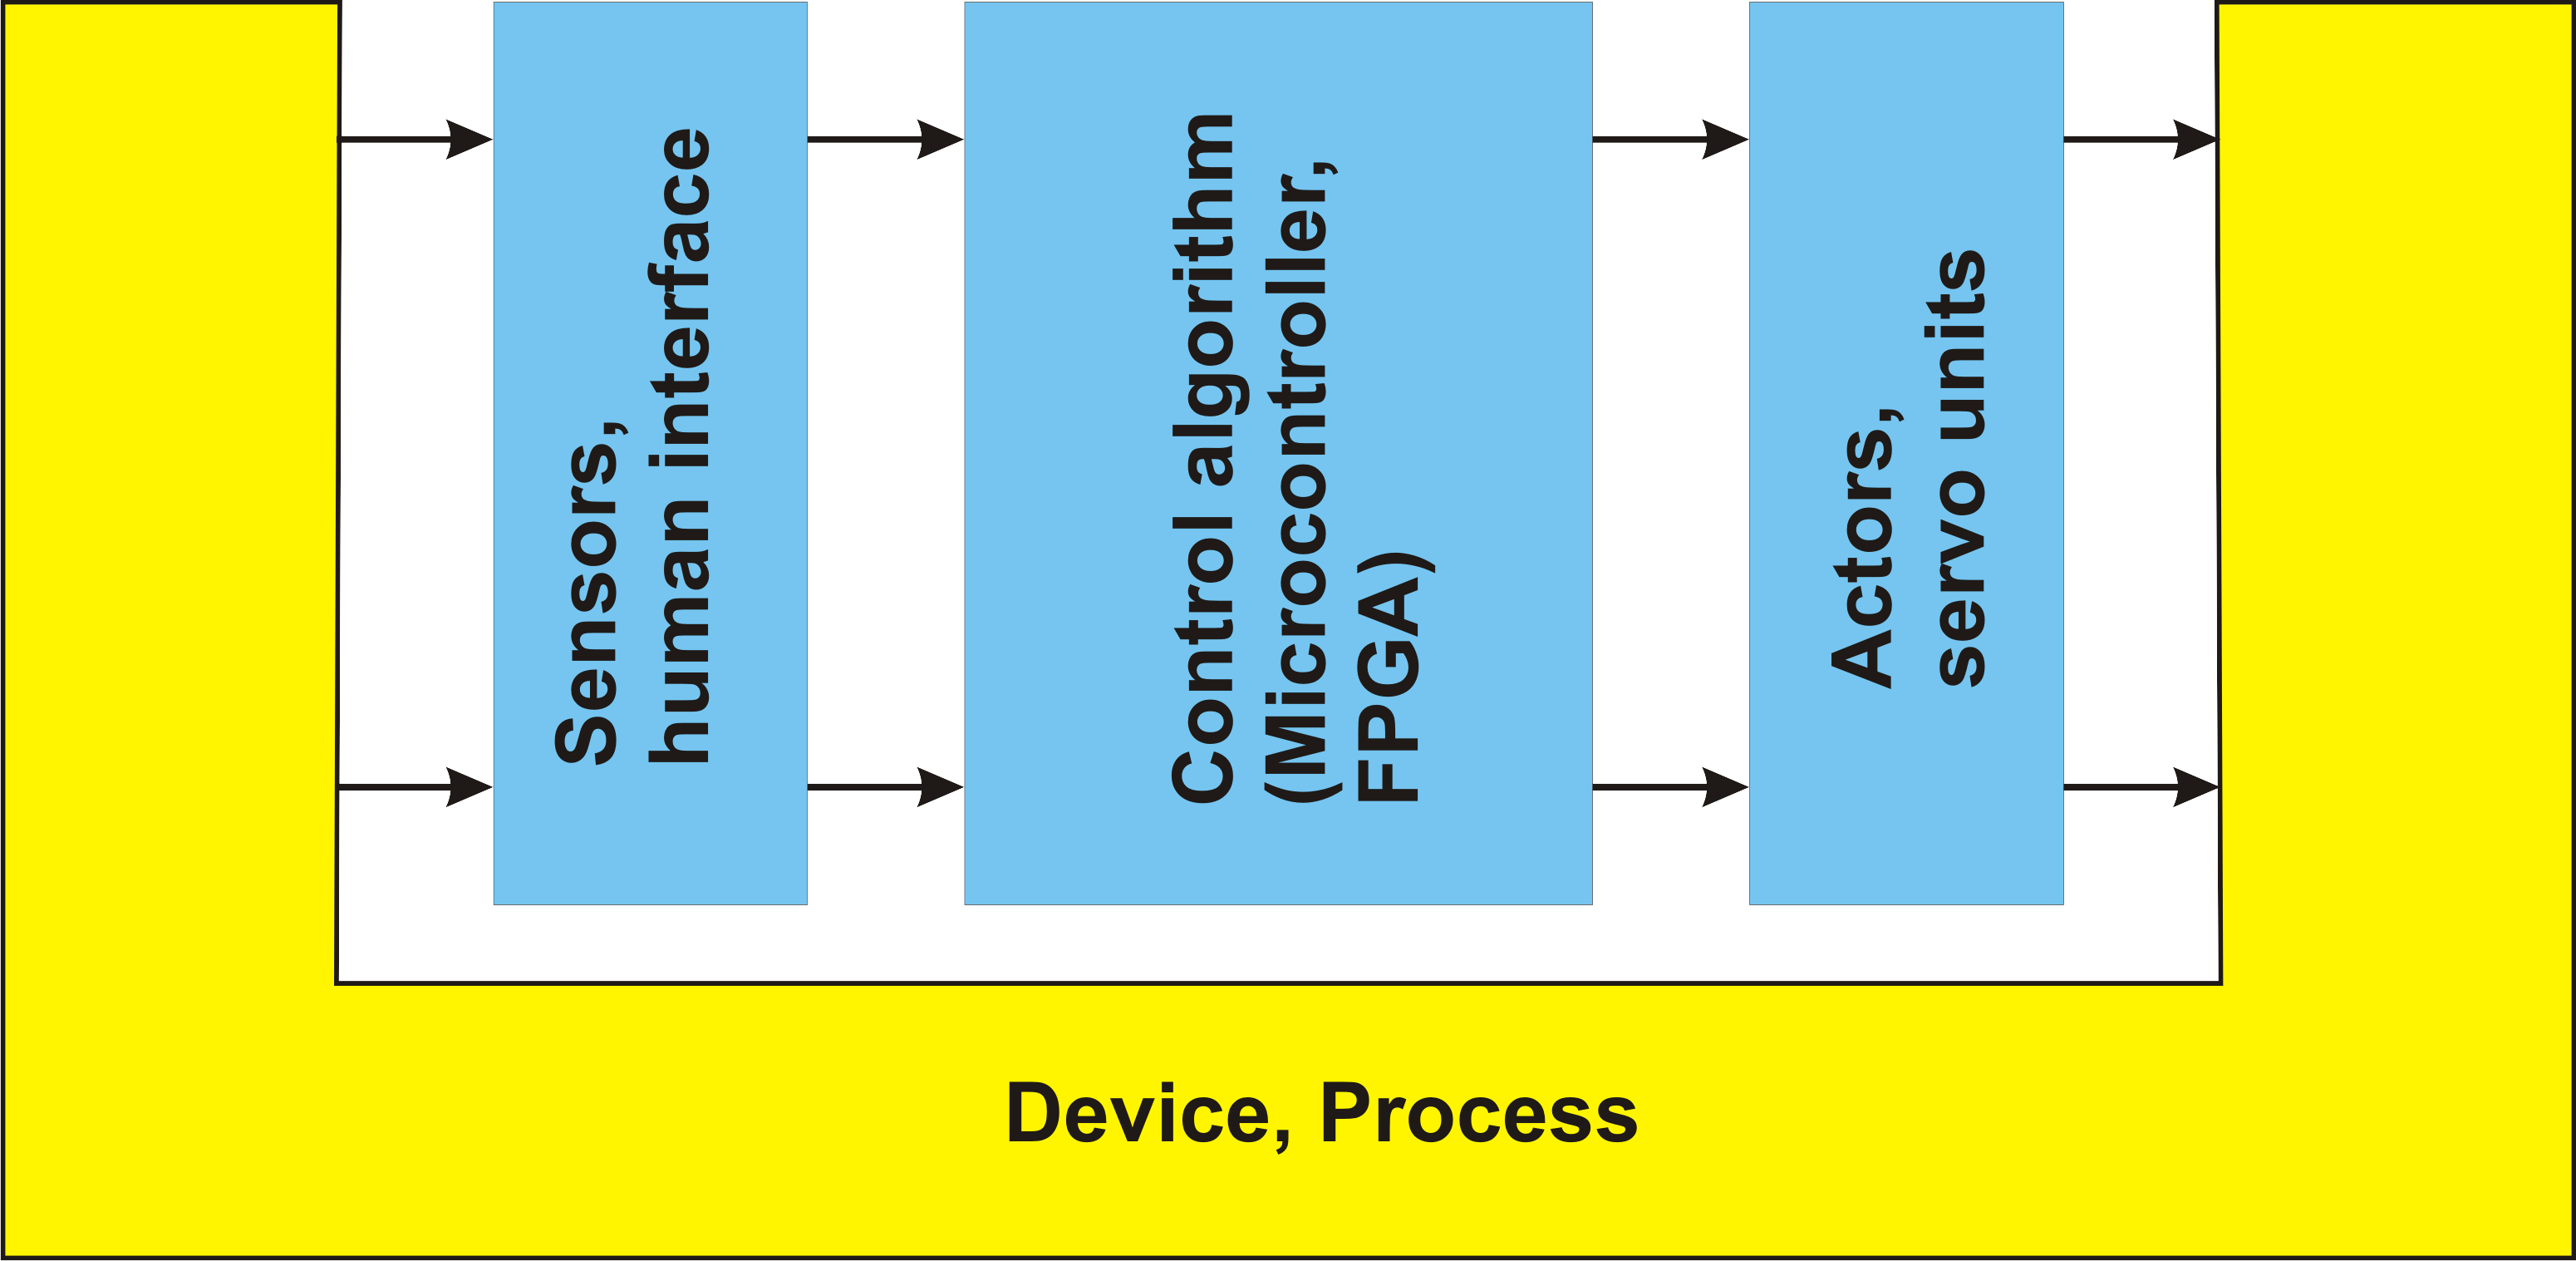
\epsfig{file=figures/Fig_1_10_Blockdiagram_Embedded_System,width=0.75\textwidth}\\
	  \caption{Block diagram of an embedded system}
     \end{center}
\end{figure}
\os{\newpage}

\begin{figure}[!hbtp]
     \begin{center}
	  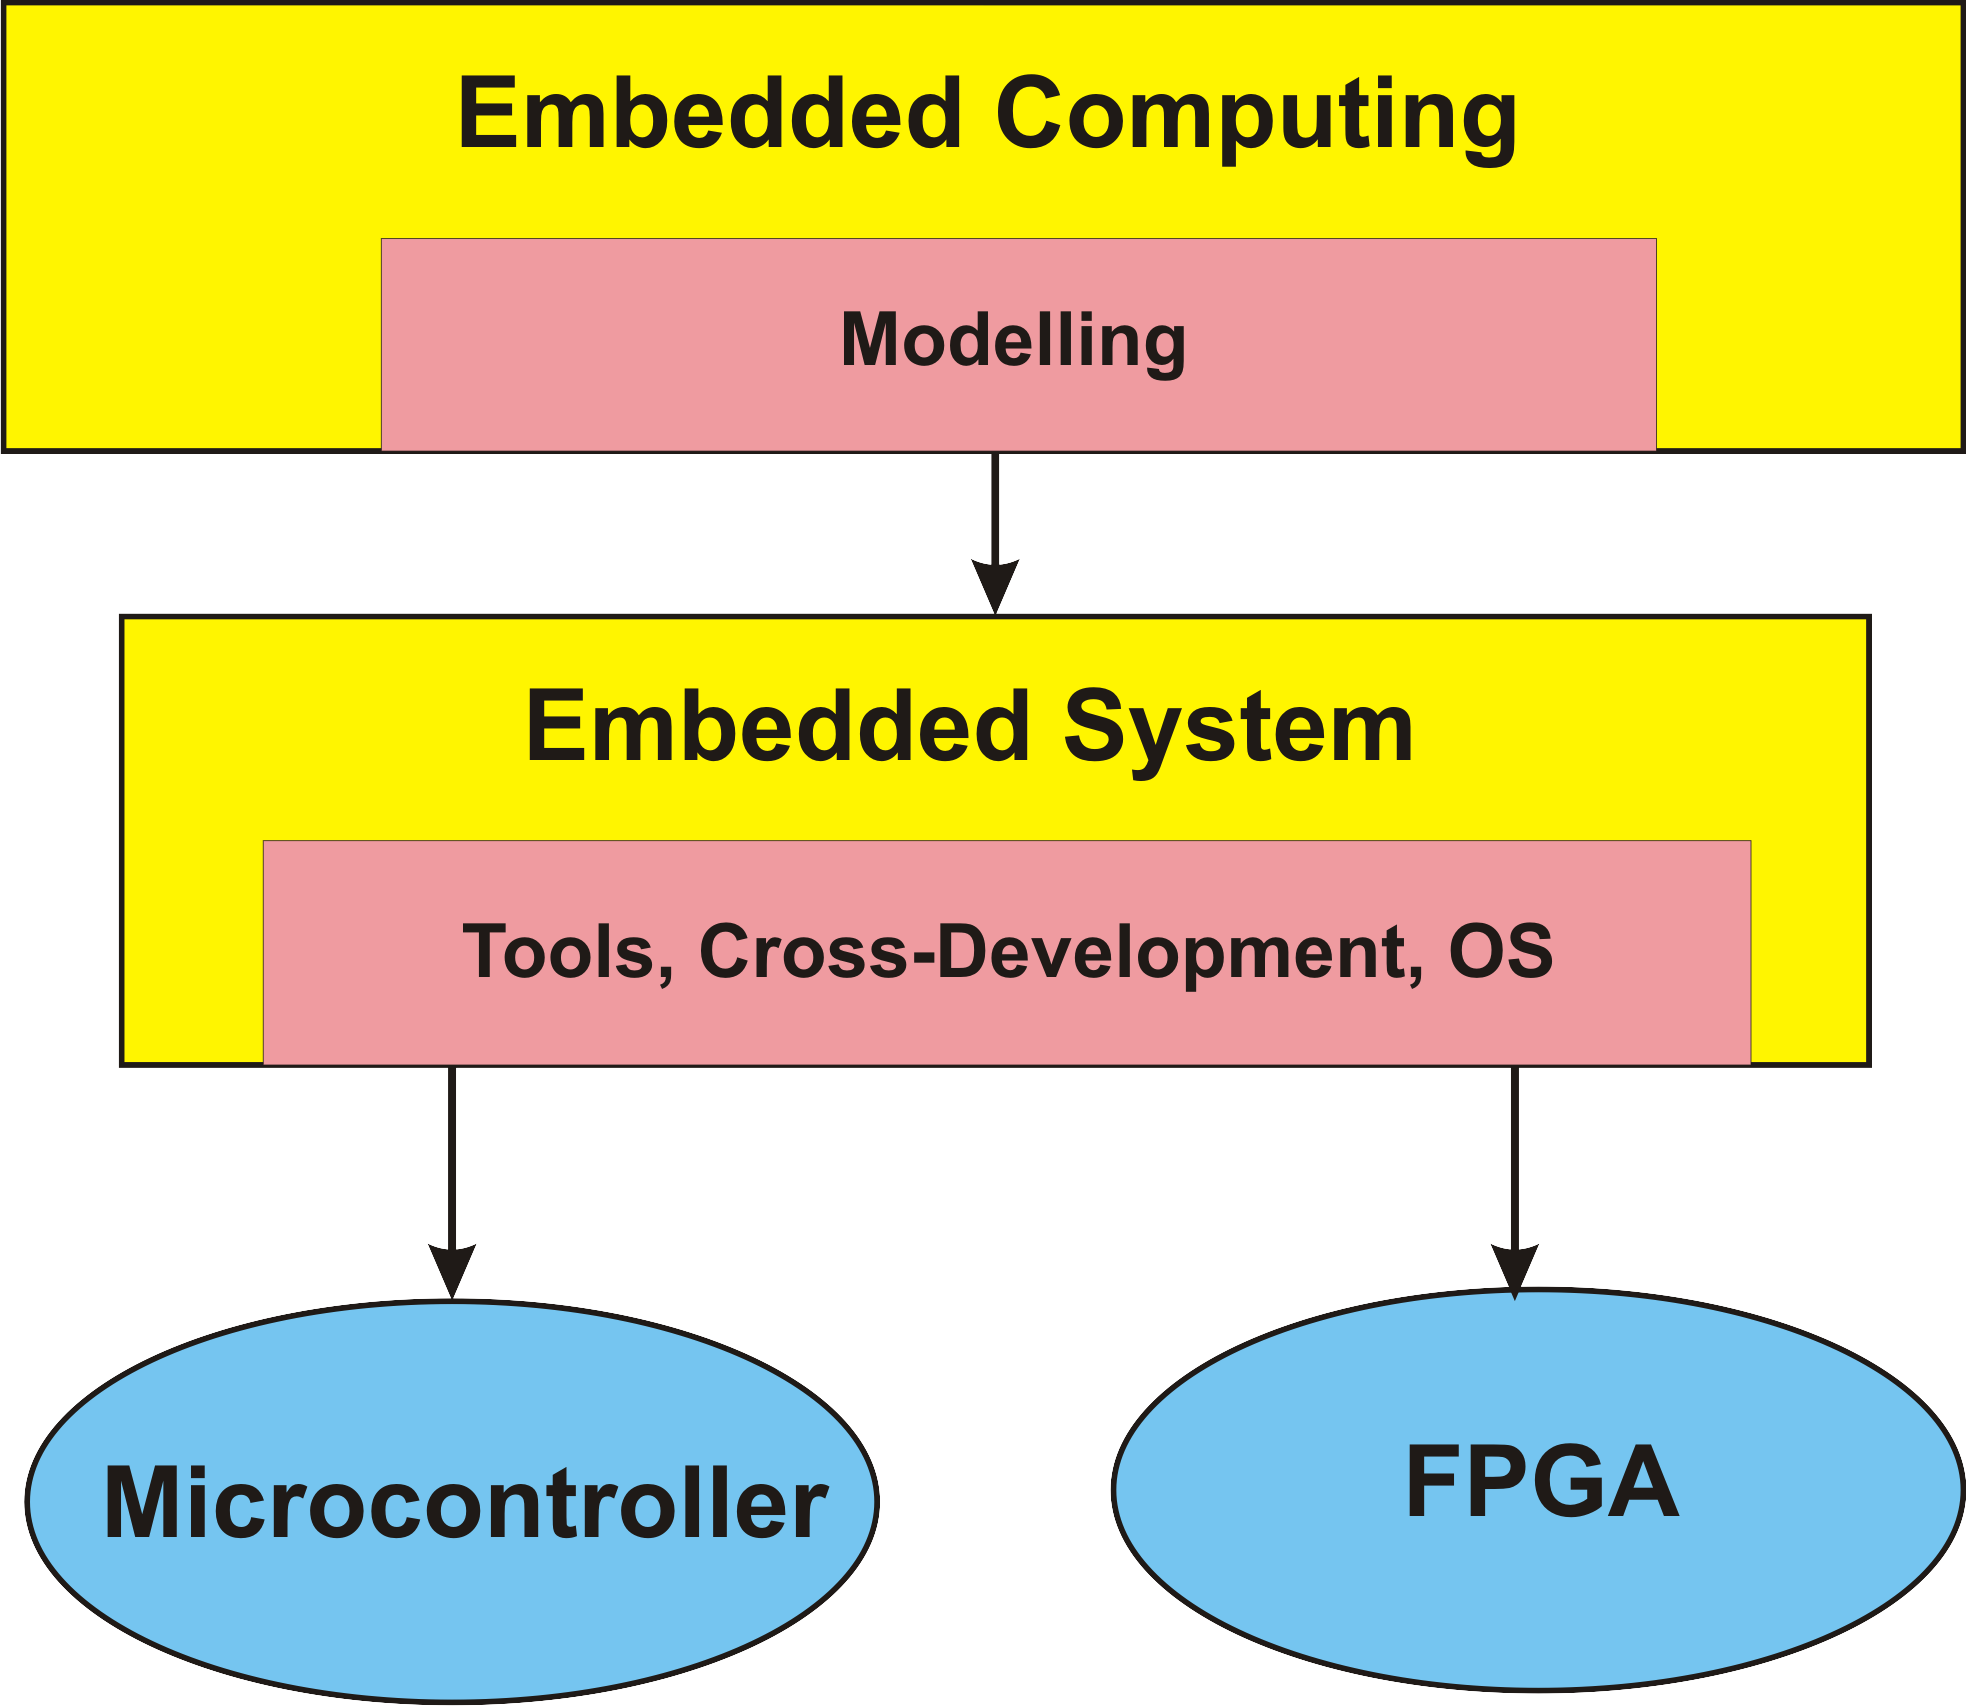
\epsfig{file=figures/Fig_1_9_Blockdiagram_Embedded_Computing,width=0.7\textwidth}\\
	  \caption{Embedded computing and the embedded system around it}
     \end{center}
\end{figure}
\os{\newpage}
\end{description}

%==============================================================================
\section{Historical Background}
%==============================================================================
\begin{description}
\item[{\rot\bf From room-sized computers to the microcontroller}]~\\[-3ex]
\begin{figure}[!hbtp]
\begin{center}
\resizebox{\textwidth}{!}{%
\begin{tikzpicture}[font=\sffamily\scriptsize,>=Stealth]
	\draw[->,thick] (0,0) -- (17.5,0);
	\foreach \x/\y/\t/\up in {
		0.3/1941/Zuse Z3: first programmable computer/1,
		1.4/1944/Harvard Mark I/0,
		2.6/1966/Apollo Guidance Computer/1,
		3.8/1971/Intel 4004: first microprocessor/0,
		5.0/1974/TMS1000: first microcontroller/1,
		6.2/1980/Intel 8051/0,
		7.4/1996/Atmel AVR/1,
		8.6/2004/ARM Cortex-M3/0,
		9.8/2005/Arduino/1,
		11.0/2010/RISC-V starts/0,
		12.2/2012/Raspberry Pi/1,
		13.4/2016/ESP32: Wi-Fi MCU/0,
		14.6/2021/RP2040/1,
		15.8/2024/RP2350: ARM or RISC-V/0} {
		\fill (\x,0) circle (2pt);
		\ifnum\up=1
			\draw (\x,0) -- (\x,0.6); \node[above,align=center,text width=16mm] at (\x,0.6) {\textbf{\y}\\\t};
		\else
			\draw (\x,0) -- (\x,-0.6); \node[below,align=center,text width=16mm] at (\x,-0.6) {\textbf{\y}\\\t};
		\fi
	}
\end{tikzpicture}}
\caption{Milestones on the way to today's embedded systems}
\end{center}
\end{figure}
\bi
	\ite the first computers (Zuse Z3 1941, Mark I 1944) filled rooms; the Apollo Guidance Computer (1966) was one of the first computers built into a vehicle
	\ite the microprocessor (1971) and the microcontroller with memory and I/O on one chip (1974) made embedded systems cheap
	\ite today a 32 bit microcontroller with Wi-Fi costs about one euro
\ei
\os{\newpage}

\item[{\rot\bf Computer generations}]~\\[-3ex]
\begin{center}
\resizebox{0.95\textwidth}{!}{%
\begin{tabular}{|c|c|c|c|}
\hline
\textbf{generation} & \textbf{period} & \textbf{technology} & \textbf{typical systems}\\
\hline
1 & 1945 -- 1955 & vacuum tubes & mainframes \\
2 & 1955 -- 1965 & transistors & mainframes, process control \\
3 & 1965 -- 1975 & integrated circuits & minicomputers \\
4 & 1975 -- & LSI / VLSI, microprocessors & workstations, PCs, microcontrollers \\
today & & systems on chip, many cores & smartphones, IoT, AI accelerators \\
\hline
\end{tabular}}
\end{center}
\bi
	\ite the trend continues: more functions on one chip, less energy per operation, lower price
	\ite \textbf{central vs.\ distributed}: instead of one central computer, many small connected controllers close to the sensors and actuators
\ei
\os{\newpage}
\end{description}

%==============================================================================
\section{Characteristics of Embedded Systems}
%==============================================================================
\begin{description}
\item[{\rot\bf Dependability}]~\\[-3ex]
\bi
	\ite \textbf{reliability}: probability that the system works correctly for a given time, provided it worked at the start
	\bi
		\ite operation for years without restart; recovery from errors by itself (watchdog)
	\ei
	\ite \textbf{maintainability}: how quickly the system works again after an error
	\ite \textbf{availability}: probability that the system works at a given time
	\ite \textbf{safety}: the system does not endanger people or the environment -- even if it fails
	\ite \textbf{security}: the system resists attacks; connected devices must be protected and updatable
\ei
\qbox{Even perfectly designed systems can fail if the assumptions about the workload and possible errors turn out to be wrong.
\newline
Dependability must be considered from the very beginning -- it cannot be added afterwards.}
\os{\newpage}

\item[{\rot\bf Efficiency}]~\\[-3ex]
\bi
	\ite \textbf{energy}: battery operation for months or years, sleep modes, energy harvesting
	\ite \textbf{code size and memory}: kilobytes instead of gigabytes; no hard disk
	\ite \textbf{run time}: real-time requirements -- a correct answer that arrives too late is wrong
	\ite \textbf{size and weight}: the electronics must fit into the device
	\ite \textbf{cost}: in a series of millions every cent counts; the development costs are spread over the number of devices
\ei
\os{\newpage}

\item[{\rot\bf Further characteristics}]~\\[-3ex]
\bi
	\ite \textbf{reactive}: continuous interaction with the environment, at its pace (chapter Modelling)
	\ite \textbf{real time}: deadlines are part of the specification (chapter Operating Systems)
	\ite \textbf{dedicated}: one purpose, known in advance -- hardware and software can be optimised for it
	\ite \textbf{heterogeneous}: hardware and software, analog and digital, different processors and networks in one system
	\ite \textbf{long lifetime}: industrial devices and cars are used for 10 to 20 years -- software must be maintained that long
	\ite \textbf{cyber-physical}: computation and physics are coupled in feedback loops (chapter Cyber-Physical Systems)
\ei
\os{\newpage}
\end{description}

%==============================================================================
\section{About this Lecture}
%==============================================================================
\begin{description}
\item[{\rot\bf Contents}]~\\[-3ex]
\begin{center}
\resizebox{0.95\textwidth}{!}{%
\begin{tabular}{|c|l|l|}
\hline
\textbf{chapter} & \textbf{topic} & \textbf{platform of the examples} \\
\hline
2 & Modelling: state machines, data flow & Pico (coffee machine FSM) \\
3 & Cyber-physical systems, Modelica & OpenModelica, Python \\
4 & Processors: AVR, Cortex-M, RISC-V & compiler output for 4 processors \\
5 & Programming: build process, assembly, C, Rust, MicroPython, debugging & Pico, PC \\
6 & Peripherals and interfaces: GPIO, interrupts, timers, ADC, UART, I$^2$C, SPI & Pico \\
7 & Networking: Wi-Fi, IP, TCP/UDP, sockets, HTTP, MQTT & ESP32-C3, PC \\
8 & Operating systems: FreeRTOS, Embassy, embedded Linux & ESP32-C3 \\
\hline
\end{tabular}}
\end{center}
\bi
	\ite every example exists in \textbf{C} and in \textbf{Rust} (some also in Python); all are in the folder \texttt{examples/} of the lecture repository
\ei
\os{\newpage}

\item[{\rot\bf Tools}]~\\[-3ex]
\bi
	\ite \textbf{Wokwi} (\url{https://wokwi.com}): simulator for Raspberry Pi Pico, ESP32, Arduino and STM32 in the browser -- with LEDs, buttons, sensors, displays, logic analyzer and Wi-Fi
	\bi
		\ite C (Arduino core + SDK) and MicroPython run directly in the browser
		\ite Rust: build locally with \texttt{cargo}, simulate with the Wokwi extension for VS Code
	\ei
	\ite \textbf{Replit} (\url{https://replit.com}) or your own PC: programs for the PC side (sockets, Python, Rust tests)
	\ite \textbf{Rust}: \texttt{rustup}, \texttt{cargo}, targets \texttt{thumbv6m-none-eabi} (Pico) and \texttt{riscv32imc-unknown-none-elf} (ESP32-C3)
	\ite \textbf{git}: all sources of the lecture and the examples are under version control
	\ite real hardware is optional: Raspberry Pi Pico and ESP32-C3 boards cost a few euros, and the same programs run on them
\ei
\os{\newpage}

\item[{\rot\bf Exercises}]~\\[-3ex]
\bi
	\ite List ten embedded systems in your home. For each: which sensors, which actuators, which communication?
	\ite Which of the characteristics (dependability, efficiency, real time, cost) is most important for an airbag control unit, a smart light bulb and a heart pacemaker?
	\ite Open \url{https://wokwi.com}, start a new Raspberry Pi Pico project and let the on-board LED blink.
\ei
\end{description}


%%%%%%%%%%%%%%%%%%%%%%%%%%%%%%%%%%%%%%%%%%%%%%%%%%%%%%%%%%%%%%%%%%%%%%%%%%
\chapter{Modeling}
%%%%%%%%%%%%%%%%%%%%%%%%%%%%%%%%%%%%%%%%%%%%%%%%%%%%%%%%%%%%%%%%%%%%%%%%%%%
\section{General Requirements}
%%%%%%%%%%%%%%%%%%%%%%%%%%%%%%%%%%%%%%%%%%%%%%%%%%%%%%%%%%%%%%%%%%%%%%%%%%%
\nsl{The most embedded systems start with integration of a small microcontroller which performs some functions which are implemented in hardware. To emulate this function only a single program or several small-size programs are necessary. There is no need to build a model and to simulate the behaviour of the emulated functions. Also the documentation for such projects is small. The development starts with the programming and stops with a successful test. Then you could forget the project and start with the next.
\newline
But with changing times embedded systems have become more complex. So the development process has to be more structured. On of the major steps involved is  the documentation. Companies spend a lot of money for documentation of embedded systems. A tool which helps the documentation process is hence a basic requirement. Model based development tools help us achieve this goal.
\newline
The next step is to overcome the special constrains of an embedded system. Real-time aspects, dead-lock situations, failure safe behaviour are requirements of any typical embedded system. A model should help us achieve these goals. This means that not only the correct result of a designed algorithm have to be tested, the results have to be in compliance of the requirements of an embedded system.
}
\bi
	\ite Classification of systems from the point of programming
\ei

\begin{figure}[!hbtp]
     \begin{center}
	  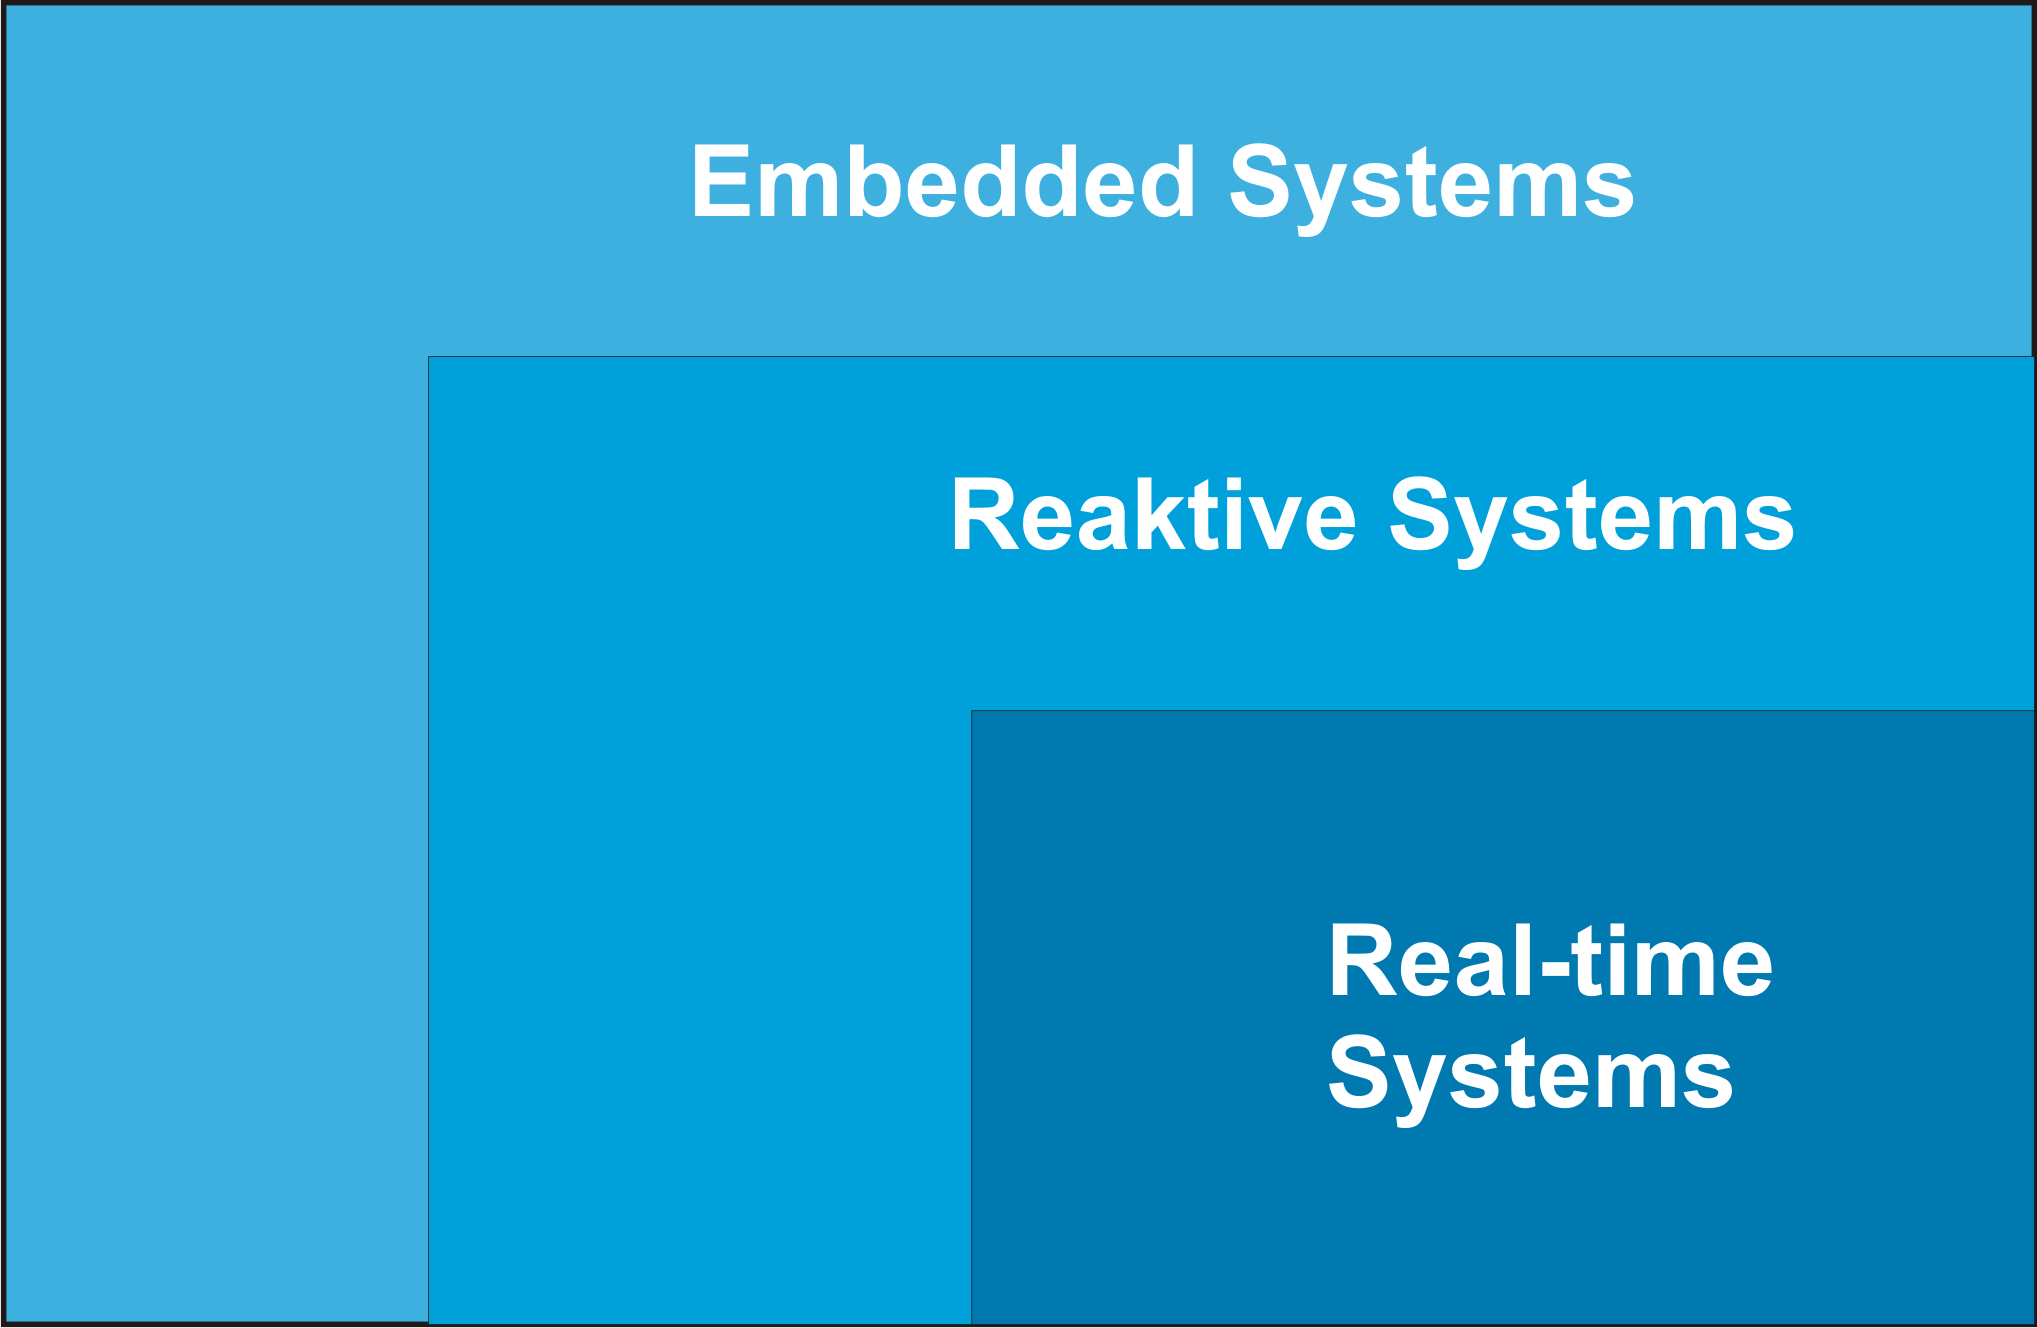
\epsfig{file=figures/Fig_2_1_Classification,width=0.7\textwidth}\\
	  \caption{Classification of embedded systems and real-time-systems}
     \end{center}
\end{figure}
\os{\newpage
}

\defn{def:embedded system}
{An \textbf{embedded system} is a special-purpose computer system designed to perform a dedicated function. Unlike a general-purpose computer, such as a personal computer, an embedded system performs one or a few pre-defined tasks, usually with very specific requirements, and often includes task-specific hardware and mechanical parts not usually found in a general-purpose computer. [Wikipedia]}


\defn{def:reaktive systems}
{``A \textbf{reactive system} is one which is in continual interaction
  with is environment and executes at a pace determined by
  that environment'' [Berg\'{e}, 1995]}

\bi
	\ite interaction with the system controlled by sensors or from the environment
	\ite specification of minimal and maximal response time
	\ite system could contain parallel and distributed parts (subsystems)
\ei

\defn{def:real-time systems}
{A \textbf{real-time system} have to give a responce as fast as required. So the system must respond to a signal, event or request fast enough to satisfy some requirement. Realtime often refers to process control and embedded systems}

\bi
	\ite a real-time operating system (RTOS) facilitates the creation of a real-time system
	\ite but real-time systems could operate without an RTOS
	\ite if a real-time system responds deterministically \pr hard real-time system
	\ite if a real-timesystem guarantees a deadline for responds \pr soft real-time system
\ei

\os{\newpage}
\begin{description}
\item[{\rot\bf Requirements }]~\\[-3ex]

\bi
	\ite concurrency \pr real-time systems are mostly concurrent
	\ite synchronization and communication \pr modeling the communication between distributed systems
	\ite portability and flexibility
	\ite programming elements \pr arithmetic operations, loops, and function calls should be available
	\ite non-standard I/O devices \pr switches, analogue and digital I/O
	\ite non-functional properties \pr e.g. fault-tolerance, disposability, EMC-properties, user friendliness, extendibility, expected life time, power consumption...
	\ite Co-Design aspects \pr modeling hard- and software functions
\ei
\item[{\rot\bf but }]~\\[-3ex]
\bi
	\ite models should be readable
	\ite models should have a hierarchical structure \pr ``humans not capable to understand systems
containing more than \begin{math} \sim \end{math} 5 objects''
\ei
\qbox{A model must be as simple as possible, but not simpler. [A. Einstein]}
\end{description}

\begin{figure}[!hbtp]
     \begin{center}
	  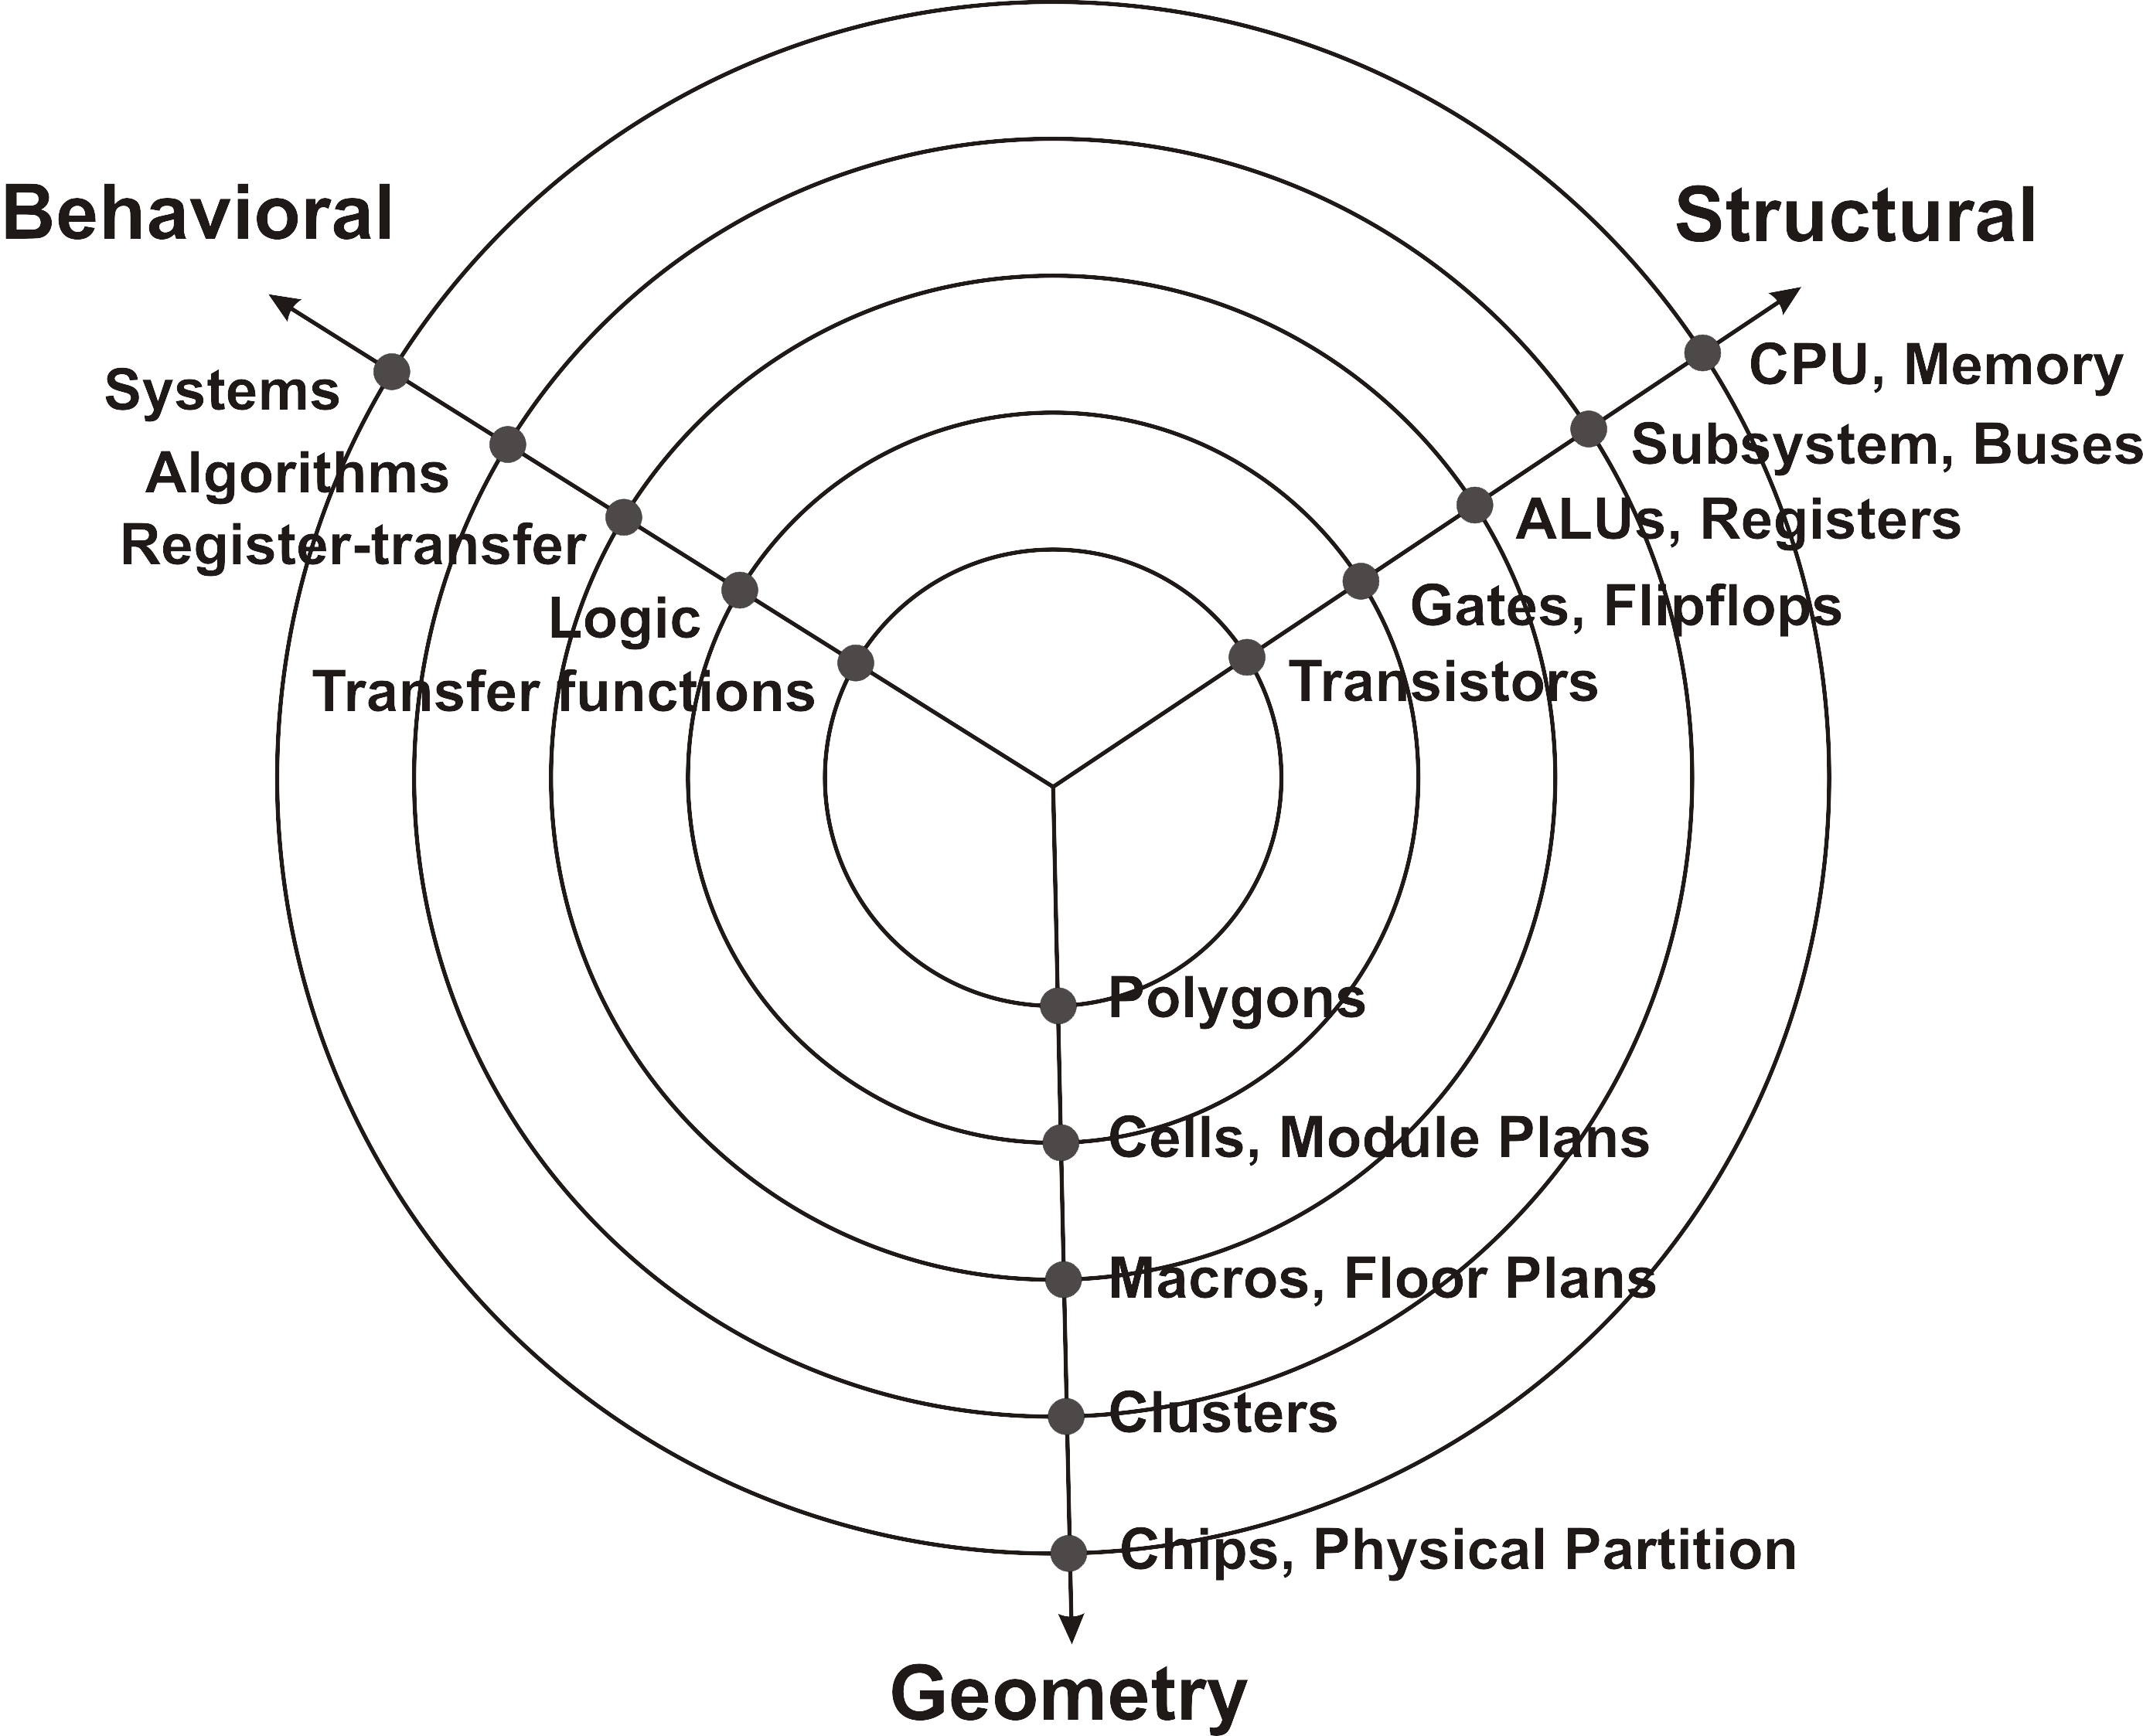
\epsfig{file=figures/Fig_2_2_Y_Chart_Gajski_Kuhn,width=0.8\textwidth}\\
	  \caption{Y-Chart from Gajski-Kuhn}
     \end{center}
\end{figure}
\os{\newpage}

\bi
	\ite a model could could change to different level in the Y-Chart
	\ite Y-Chart are focused on the hardware-design
	\ite concurrency and time behavior difficult to modeling
\ei

\begin{figure}[!hbtp]
     \begin{center}
	  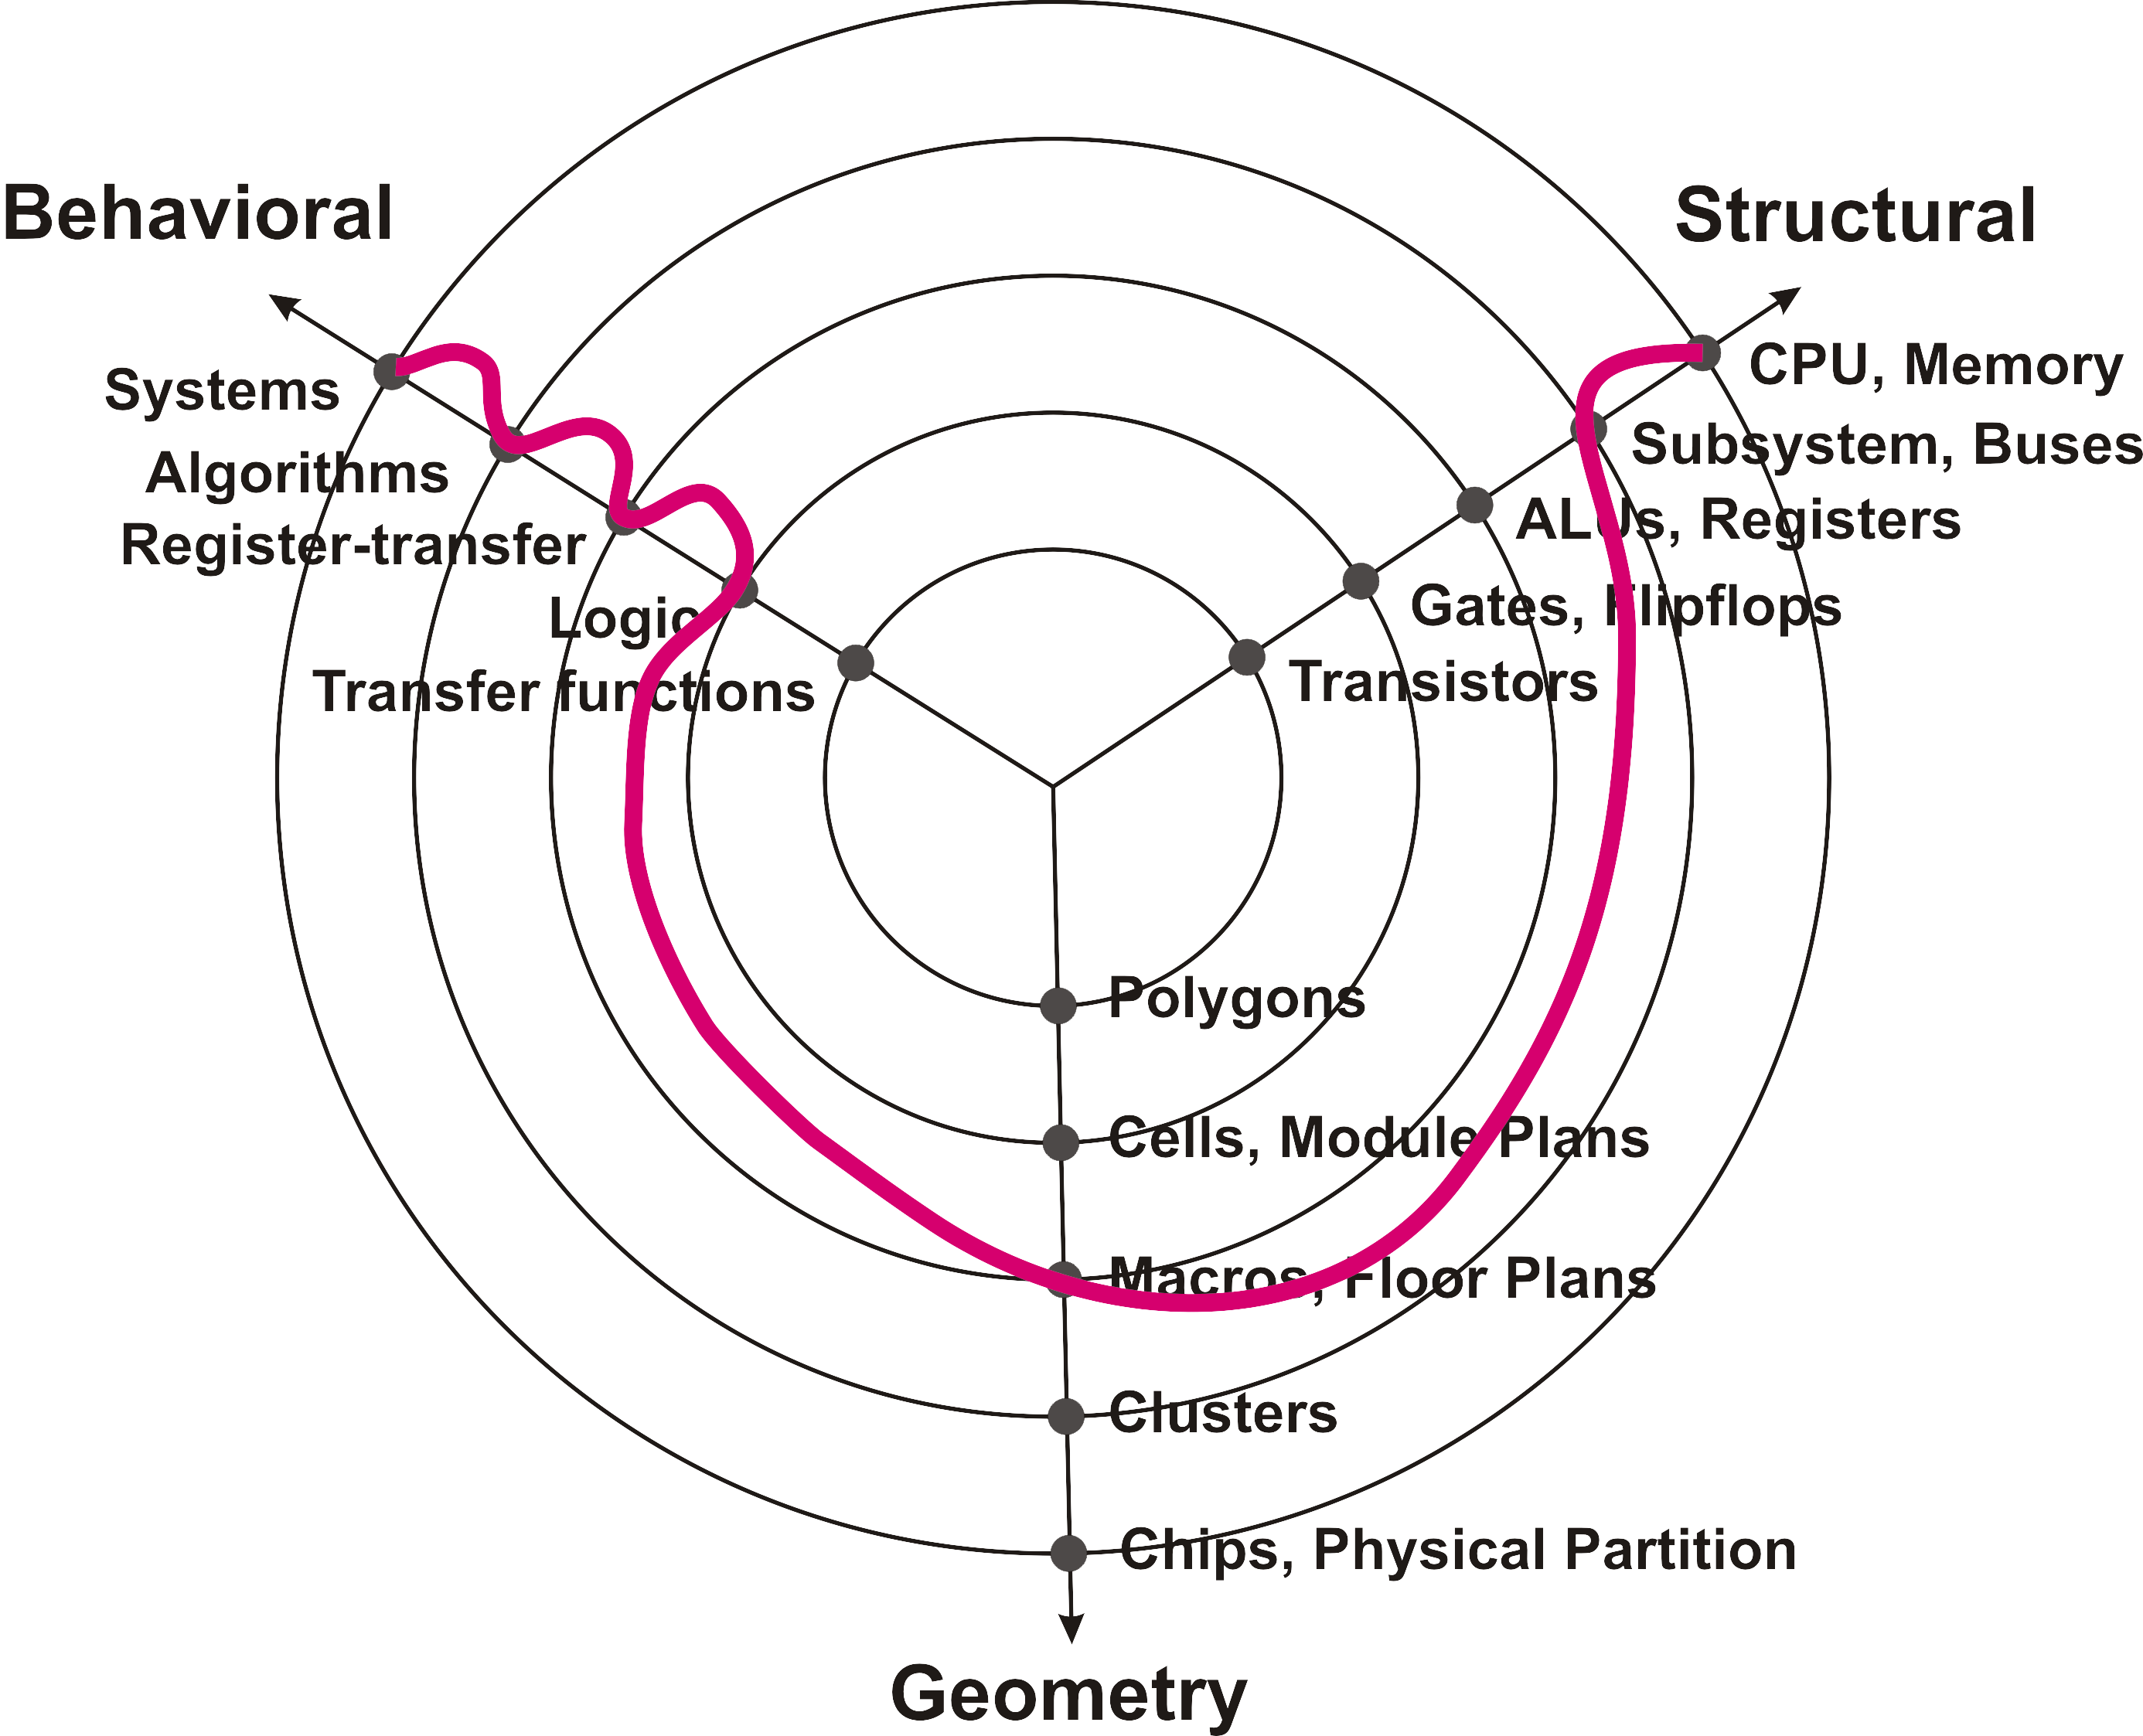
\epsfig{file=figures/Fig_2_3_Different_Level_Y_Chart,width=0.5\textwidth}\\
	  \caption{Different levels in a Y-Chart}
     \end{center}
\end{figure}
\os{\newpage}

\begin{figure}[!hbtp]
     \begin{center}
	  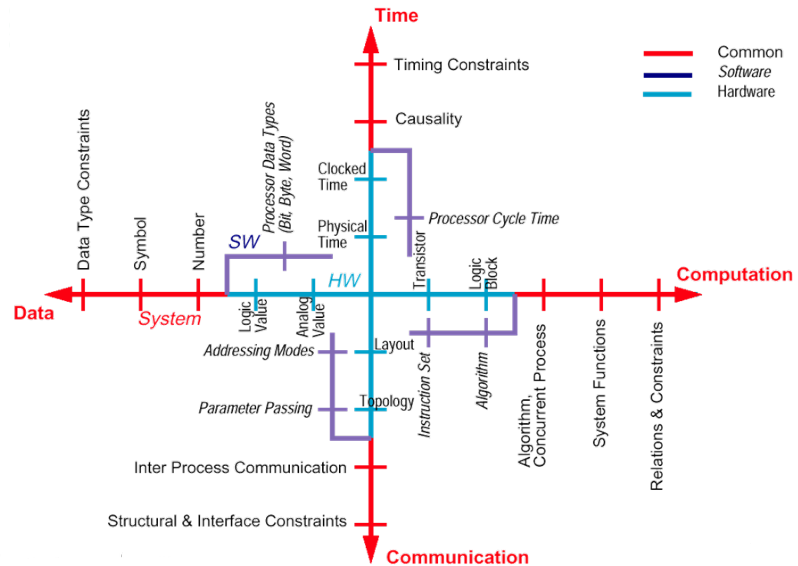
\epsfig{file=figures/Fig_2_4_4_D_CoDesign,width=0.9\textwidth}\\
	  \caption{Hardware and Software Co-Design}
     \end{center}
\end{figure}
\os{\newpage}

\begin{description}
\item[{\rot\bf Design methods }]~\\[-3ex]
\bigskip
\bi
	\ite capture and simulate
	\bi
		\ite specification of the embedded system (development)
		\ite generation of block diagrams (details not spezified)
		\ite simulation and verification
	\ei
\bigskip
	\ite describe and synthesize
	\bi
		\ite generate functions (software and hardware) from CAD-tools
		\ite logic synthesis as an integral component of the draft
		\ite use of hardware description languages (like VHDL)
	\ei
\bigskip
	\ite specify-explore-refine
	\bi
		\ite CAD/CASE-tools supports the explore-step (verification of different alternatives)
		\ite unfortunately these steps are not supported for all levels of the Co-Design
	\ei
\ei
\end{description}
\os{\newpage}
\begin{description}
\item[{\rot\bf Different views on a model }]~\\[-3ex]
\bigskip
\bi
	\ite  behavioral view
	\bi
		\ite use models or part of models as black boxes
		\ite focus on states, processes, procedures
	\ei
\bigskip
	\ite structural view
	\bi
		\ite specify the implementation of the system (e.g.connection of the components implies the behavior of the system)
		\ite processors, racks, printed circuit boards in the foreground
	\ei
\bigskip
	\ite view on physical components
	\bi
		\ite specify the physical characteristics of the components (e.g. expansion, layer, physical characteristics of the connections)
	\ei
\ei
\end{description}

\os{\newpage}
\begin{description}
\item[{\rot\bf Classification of models }]~\\[-3ex]
\bigskip
	\bi
		\ite a model which fulfils all the requirements of embedded system doesn't exit
		\ite actual models are focused on specific aspects
		\os{\bigskip}
		\bi
			\ite state space oriented
			\os{\bigskip}
			\ite activity oriented
			\os{\bigskip}
			\ite structural oriented
			\os{\bigskip}
			\ite data driven oriented
			\os{\bigskip}
			\ite heterogeneous oriented
		\ei
	\ei
\end{description}

%%%%%%%%%%%%%%%%%%%%%%%%%%%%%%%%%%%%%%%%%%%%%%%%%%%%%%%%%%%%%%%%%%%%%%%%%%%
\section{State Space Oriented Models}
%%%%%%%%%%%%%%%%%%%%%%%%%%%%%%%%%%%%%%%%%%%%%%%%%%%%%%%%%%%%%%%%%%%%%%%%%%%
\bigskip
\bi
	\ite Classical automata (FSM, \underline{f}inite \underline{s}tate \underline{m}achine) are state space models
	\ite Two different versions: Moore- and Mealy-Automata
\ei

\begin{figure}[!hbtp]
     \begin{center}
	  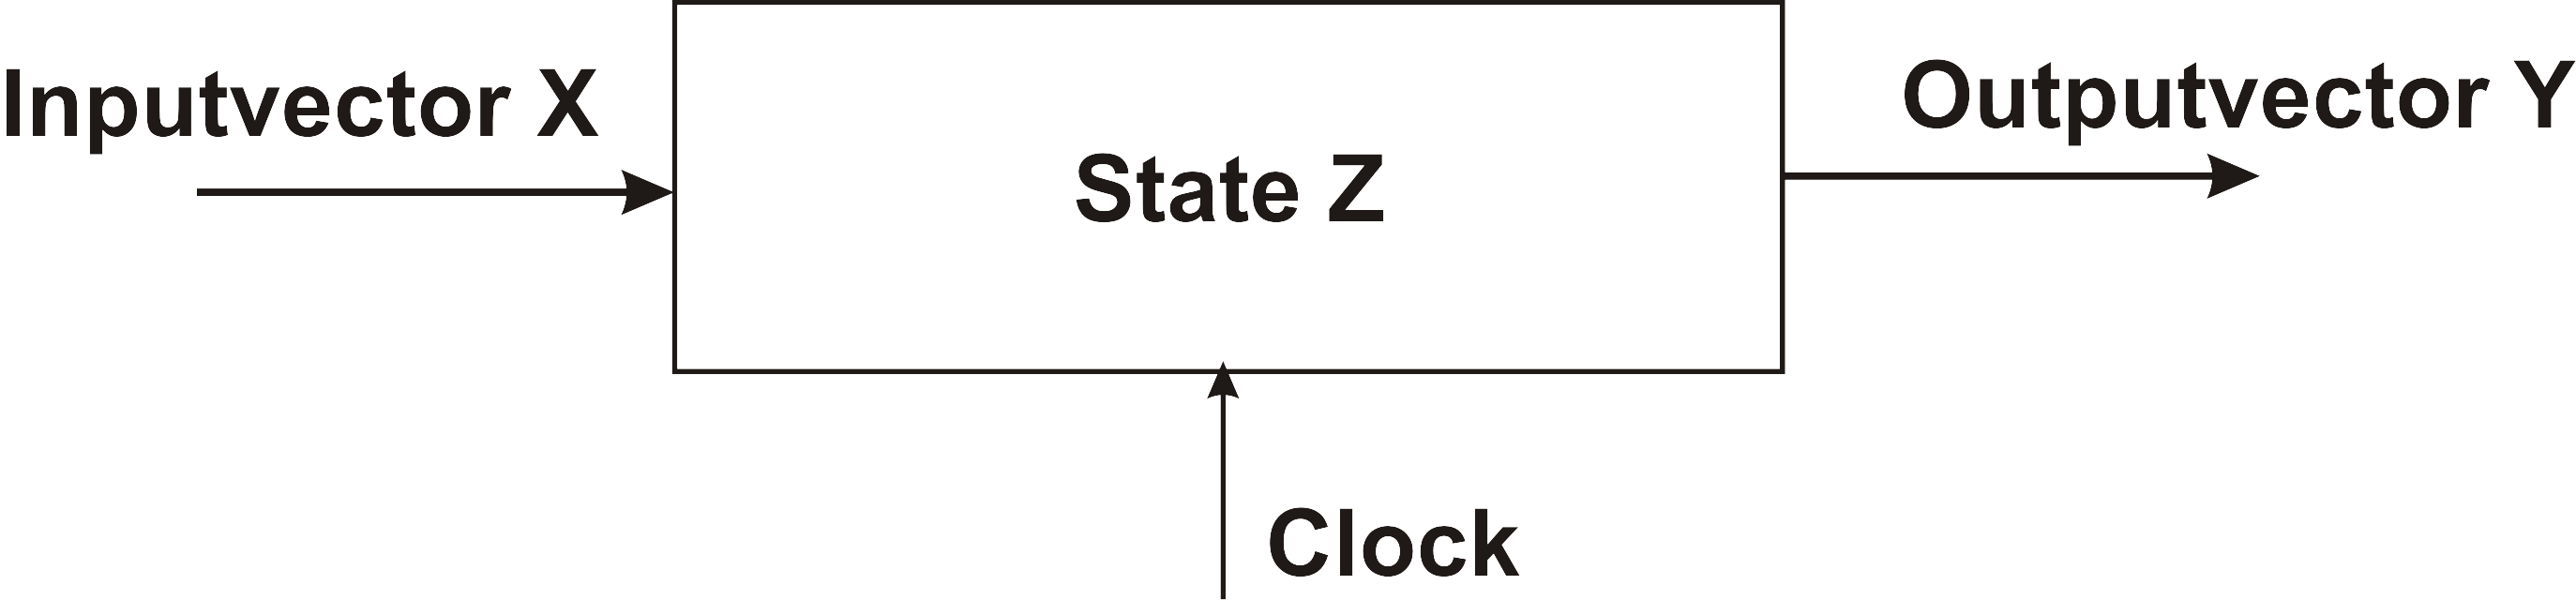
\epsfig{file=figures/Fig_2_5_FSM,width=0.9\textwidth}\\
	  \caption{Blockdiadram of a FSM}
     \end{center}
\end{figure}

\os{\newpage}

\begin{eqnarray*}
&Moore - automata\\
&Y = \lambda (Z); \ Z^{+} = \delta(X,Z)\\
\\
&Mealy - automata\\
&Y = \lambda(X,Z); \ Z^{+} = \delta(X,Z)\\
\\
&\lambda = output-function\\
&\delta = computes \ the \ next \ state \ Z^{+}
\end{eqnarray*}
\os{\newpage}

\begin{figure}[!hbtp]
     \begin{center}
	  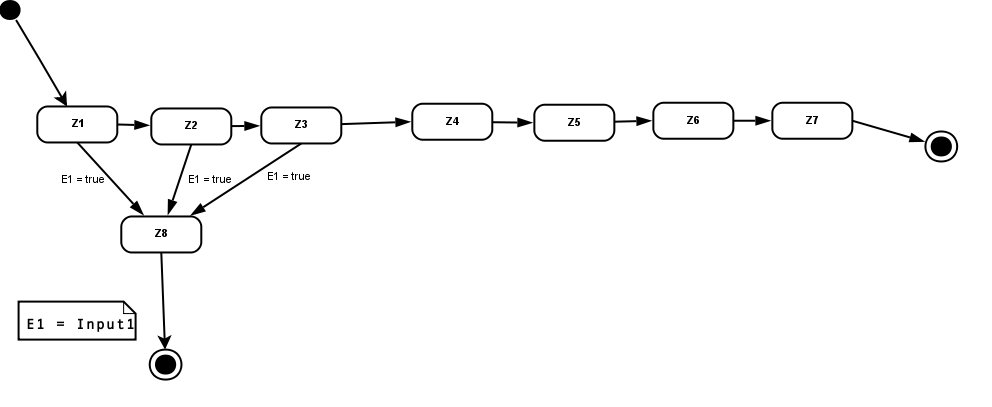
\epsfig{file=figures/Fig_2_6_FSM_Detail,width=0.8\textwidth}\\
	  \caption{FSM more in detail}
     \end{center}
\end{figure}

\os{\newpage}
\bi
	\ite FSM not useful for complex systems (to much details)
	\ite Introduction of hierarchy in the FSM \pr StateCharts [Harel, 1987]
\ei

\begin{figure}[!hbtp]
     \begin{center}
	  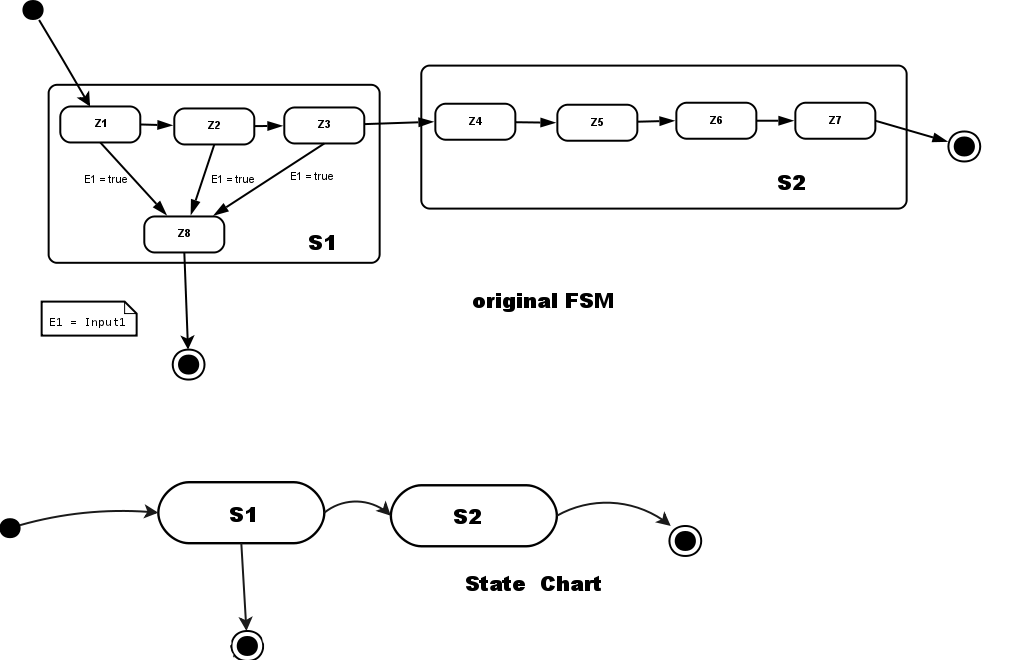
\epsfig{file=figures/Fig_2_7_State_Chart,width=0.7\textwidth}\\
	  \caption{State Chart}
     \end{center}
\end{figure}
\os{\newpage}

\defn{def:State Chart}
{Current states of FSMs are called \textbf{active states}.\\
States which are not composed of other states are called \textbf{basic
states}.\\
States containing other states are called \textbf{super-states}.\\
Super-states S are called \textbf{OR-super-states}, if exactly one of the
sub-states of S is active whenever S is active.}

\begin{figure}[!hbtp]
     \begin{center}
	  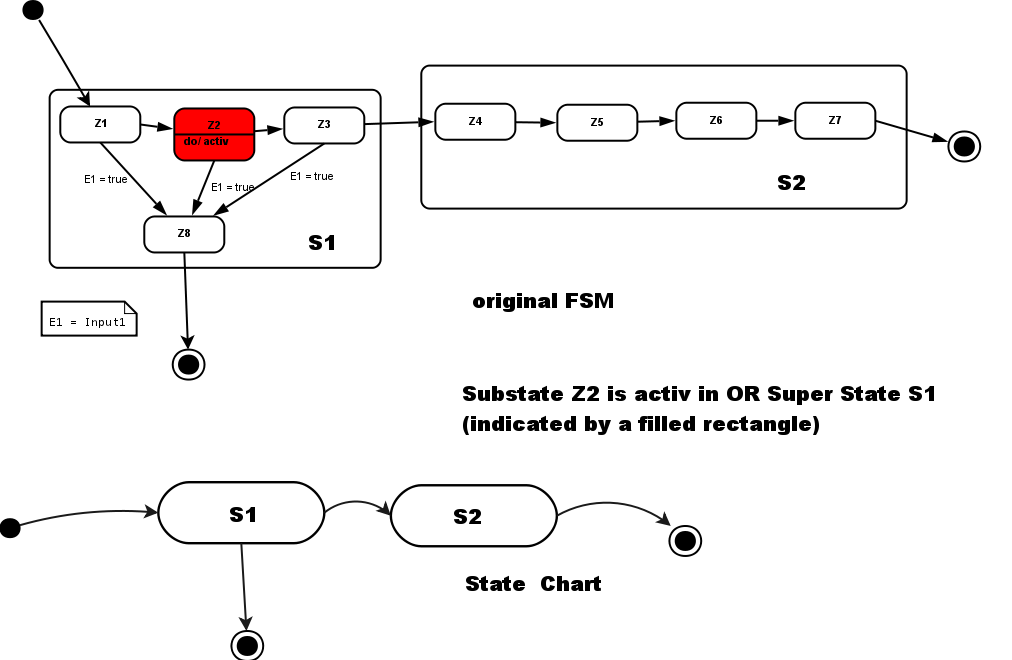
\epsfig{file=figures/Fig_2_8_Activ_Substate,width=0.6\textwidth}\\
	  \caption{Active Substate in a Super-State}
     \end{center}
\end{figure}

\os{\newpage}
\bi
	\ite In a OR-super-state only one sub-state is active
	\ite Modeling of concurrency not possible
\ei

\defn{def:AND-super-state}{A Super-states S are called \textbf{AND-super-states}, if in every AND-super-states exactly one sub-states is active.}


\begin{figure}[!hbtp]
     \begin{center}
	  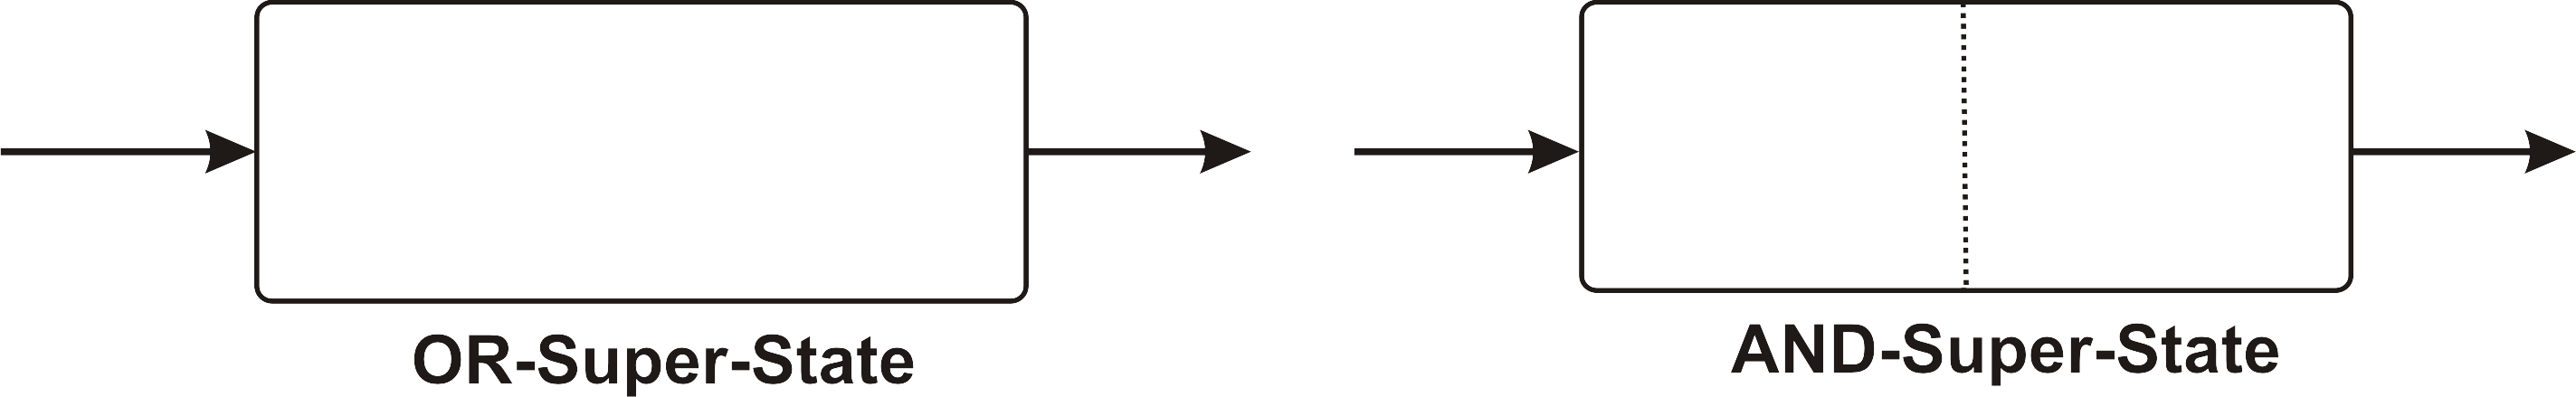
\epsfig{file=figures/Fig_2_9_OR_AND_Super_States,width=0.8\textwidth}\\
	  \caption{Concurrency in a AND-Super-State}
     \end{center}
\end{figure}
\os{\newpage}

\bi
	\ite In a AND-super-state \pr modeling of concurrent FSM possible
	\ite Implementation of a AND-super-state with a ``Product-FSM''
\ei

\begin{figure}[!hbtp]
     \begin{center}
	  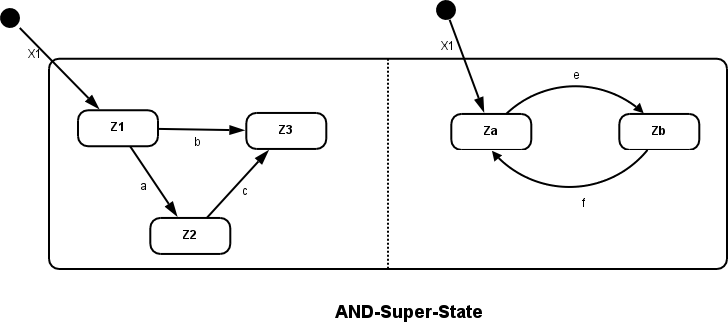
\epsfig{file=figures/Fig_2_10_AND_Superstate,width=0.8\textwidth}\\
	  \caption{Example of a AND-Super-State}
     \end{center}
\end{figure}

\os{\newpage}

\begin{figure}[!hbtp]
     \begin{center}
	  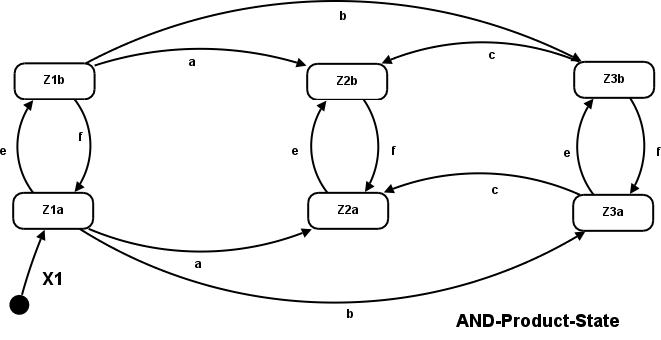
\epsfig{file=figures/Fig_2_10_AND_Product,width=0.9\textwidth}\\
	  \caption{Decomposition of a AND-Super-State}
     \end{center}
\end{figure}
\os{\newpage}

\bi
	\ite \textbf{Advantages of state charts modeling}
	\bi
		\ite hierarchy allows arbitrary nesting of AND- and OR-super
  states.
  		\ite semantics defined in a follow-up paper to original paper.
  		\ite large number of commercial simulation tools available (\textbf{StateMate, StateFlow, BetterState, ...})
		\ite some "back-ends" translate StateCharts into C or VHDL, thus enabling software or hardware implementations
	\ei
	\bigskip
	\ite \textbf{Disadvantages}
	\bi 	
		\ite generated C programs frequently inefficient
		\ite not useful for distributed applications
		\ite no program constructs
		\ite no description of non-functional behavior
		\ite no object-orientation
		\ite no description of structural hierarchy.
	\ei
\ei

\os{\newpage}
\bi
	\ite \textbf{Implementation of a Statemachine in C}
	\bi
		\ite As an example we take a coffee machine
        \ite State changes are caused by inputs (left/right/ready/!ready)
        \ite Output is not State Change -> Moore Machine		
	\ei
\ei
	\bigskip
	\begin{figure}[!hbtp]
     \begin{center}
	  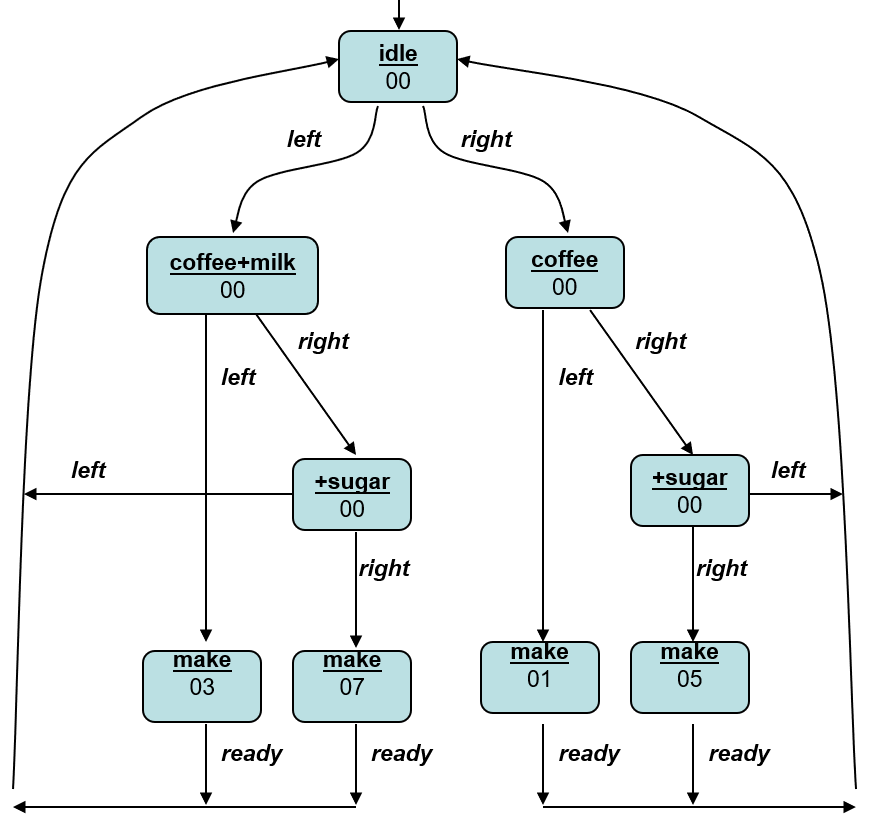
\epsfig{file=figures/Fig_2_10_CoffeeMachine_FSM,width=0.4\textwidth}\\
	  \caption{Coffee Machine FMS}
     \end{center}
\end{figure}

\os{\newpage}
\bi
	\ite \textbf{State Transition Table}
	
\ei
	\bigskip
	\begin{figure}[!hbtp]
     \begin{center}
	  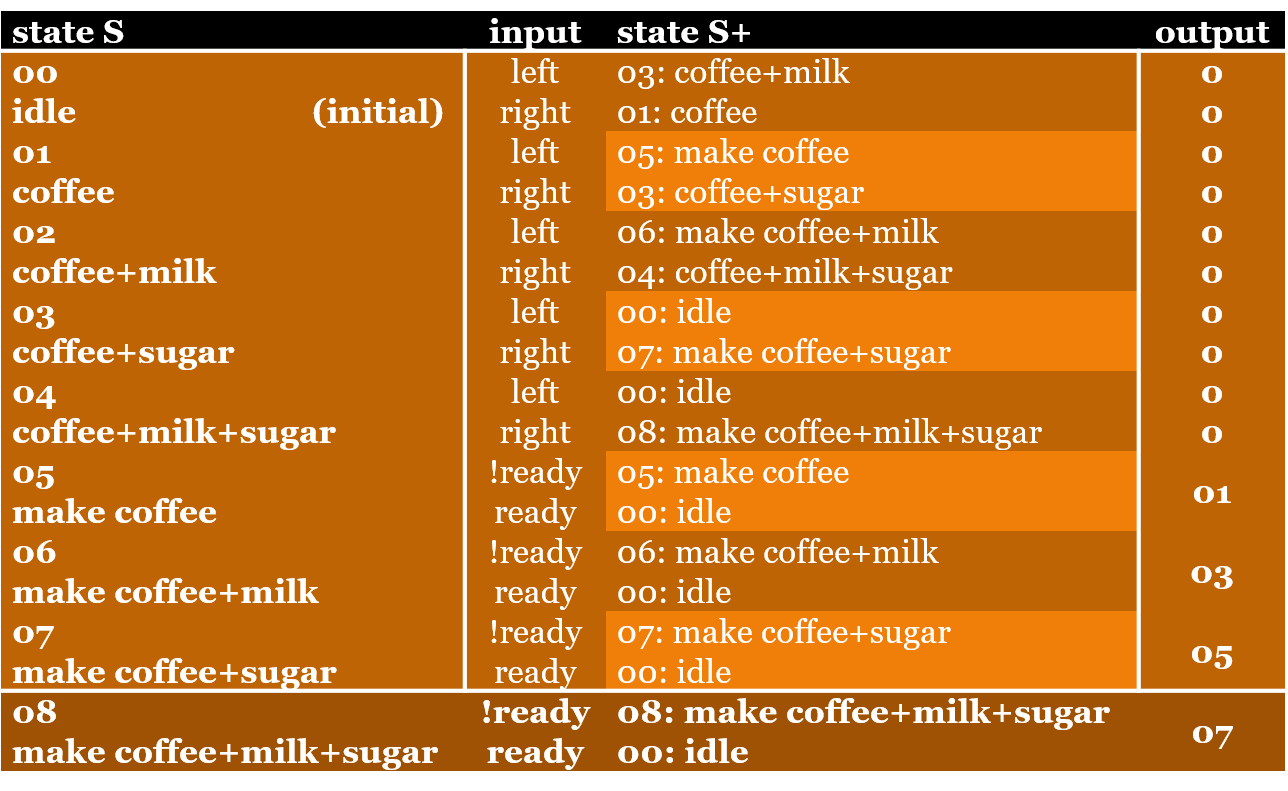
\epsfig{file=figures/Fig_2_10_CoffeeMachine_StateTable,width=0.7\textwidth}\\
	  \caption{Coffee Machine State Transition Table}
     \end{center}
\end{figure}

\os{\newpage}
\bi
	\ite \textbf{C Code - Definition of States}
	\bi
		\ite Always use ENUM to define states
        \ite Define an initial State	
	\ei
\ei
\begin{lstlisting}[language=C]
// --------------------------------------------------------
// the FSM states for the Coffee Automata
// --------------------------------------------------------
enum {  FSM_STATE_IDLE,  FSM_STATE_COFFEE, 		
        FSM_STATE_COFFEE_MILK,FSM_STATE_COFFEE_SUGAR,
        FSM_STATE_COFFEE_MILK_SUGAR,FSM_STATE_MAKE_COFFEE,
        FSM_STATE_MAKE_COFFEE_MILK, FSM_STATE_MAKE_COFFEE_SUGAR,
        FSM_STATE_MAKE_COFFEE_MILK_SUGAR,
};
// --------------------------------------------------------
int fsm_state = FSM_STATE_IDLE;
// --------------------------------------------------------
// --------------------------------------------------------
// the FSM outputs one for each state(Moore Automata model)
// --------------------------------------------------------
const int fsm_output[NUM_FSM_STATES] = {
        // output is fsm_output[fsm_state]
		0, 0, 0, 0, 0, 1, 3, 5 ,7								
        // bit0: add coffee, bit1: add milk, bit2: add sugar
 };
\end{lstlisting}

\os{\newpage}
\bi
	\ite \textbf{C Code - Inputs and Outputs}
	\bi
		\ite If possible use ENUM again	
	\ei
\ei
\begin{lstlisting}[language=C]
// --------------------------------------------------------
// the FSM outputs one for each state(Moore Automata model)
// --------------------------------------------------------
const int fsm_output[NUM_FSM_STATES] = {
        // output is fsm_output[fsm_state]
		0, 0, 0, 0, 0, 1, 3, 5 ,7								
        // bit0: add coffee, bit1: add milk, bit2: add sugar
 };
// ---------------------------------------------------------
// the FSM inputs
// ---------------------------------------------------------
enum {FSM_INP_NONE=0, FSM_INP_LEFT, FSM_INP_RIGHT, FSM_INP_READY };

\end{lstlisting}

\os{\newpage}
\bi
	\ite \textbf{C Code - State Transition}
	\bi
		\ite This function is called periodically
        \ite The period defines the response time of the system to input	
	\ei
\ei
\begin{lstlisting}[language=C]
int fsm_tic(int fsm_inp) // called periodically e.g. each 50 ms
{
	// the FSM transients realizing the state transient table
	// ------------------------------------------------------------
	switch (fsm_state) {
	case FSM_STATE_IDLE:
		if (fsm_inp == FSM_INP_LEFT) fsm_state = FSM_STATE_COFFEE;
		if (fsm_inp == FSM_INP_RIGHT) fsm_state = FSM_STATE_COFFEE_MILK;
		break;	
	case FSM_STATE_COFFEE:
		if (fsm_inp == FSM_INP_LEFT) fsm_state = FSM_STATE_MAKE_COFFEE;
		if (fsm_inp == FSM_INP_RIGHT) fsm_state = FSM_STATE_COFFEE_SUGAR;
		break;
	case FSM_STATE_COFFEE_MILK:
		if (fsm_inp == FSM_INP_LEFT) fsm_state = FSM_STATE_MAKE_COFFEE_MILK;
		if (fsm_inp == FSM_INP_RIGHT) fsm_state = FSM_STATE_COFFEE_MILK_SUGAR;
		break;
	case FSM_STATE_COFFEE_SUGAR:
		if (fsm_inp == FSM_INP_LEFT) fsm_state = FSM_STATE_IDLE;
		if (fsm_inp == FSM_INP_RIGHT) fsm_state = FSM_STATE_MAKE_COFFEE_SUGAR;
		break;
    case FSM_STATE_COFFEE_MILK_SUGAR:
		if (fsm_inp == FSM_INP_LEFT) fsm_state = FSM_STATE_IDLE;
		if (fsm_inp == FSM_INP_RIGHT) fsm_state = FSM_STATE_MAKE_COFFEE_MILK_SUGAR;
		break;
	case FSM_STATE_MAKE_COFFEE:   //here we wait for the coffeemaking to finish (ready!)
	case FSM_STATE_MAKE_COFFEE_MILK:
	case FSM_STATE_MAKE_COFFEE_SUGAR:
	case FSM_STATE_MAKE_COFFEE_MILK_SUGAR:
		if (fsm_inp == FSM_INP_READY) fsm_state = FSM_STATE_IDLE;
		break;
	default:
		;		// no state change
	}
	OUTPUT(fsm_output[fsm_state]);		// Moore FSM: one output per state
	return fsm_state;
}
\end{lstlisting}

\os{\newpage}
\bi
	\ite \textbf{Recipe for realizing a Moore Statemachine}
	\bi
		\ite Analyze the problem before coding plot a state diagram define the states
        \ite Use enums to encode states in a well readable form
        \ite Define outputs as enums with suitable encoding e.g. as bit-fields
        \ite Define input conditions causing the state transitions as enums as well
        \ite Realize a periodicaly called fsm-tic function realize transients and outputs
	\ei
\ei

\os{\newpage}
\bi
	\ite \textbf{Some Tools for creating and testing State Machines}
	\bi
		\ite The purpose of this list is not to give an exhaustive list of tools
        \ite The first part contains browserbased and free to use (at least with restrictions)
        \ite The second part contains free but installed tools
        \ite The final part commercial tools
        \ite
        \ite Browser based tools:
        \bi
            \ite Online Visual Paradigm - Commercial, with free option here:
            \ite https://online.visual-paradigm.com/app/diagrams/\#diagram:proj=0\&type=StateMachineDiagram
            \ite Nice editor
            \ite
            \ite Draw.Io - Free- Now located at
            \ite https://app.diagrams.net/
            \ite Many different options
            \ite
            \ite State Machine Simulator
            \ite http://ivanzuzak.info/noam/webapps/fsm\_simulator/
            \ite Powerful, complex editor and simulator/tester for FSM
        \ei
        \ite Free tools:
        \bi
            \ite Open Modelica available as part of the language and extensions in StateGraph
            \ite https://build.openmodelica.org/Documentation/Modelica.StateGraph.html
            \ite Powerful simulation, more complex, good integration for co-simulation
        \ei
        \ite Commercial tools:
        \bi
            \ite Matlab / Simulink Stateflow library
            \ite https://de.mathworks.com/products/stateflow.html
            \ite Powerful simulation, more complex, good integration into other libraries
        \ei
	\ei
\ei

%%%%%%%%%%%%%%%%%%%%%%%%%%%%%%%%%%%%%%%%%%%%%%%%%%%%%%%%%%%%%%%%%%%%%%%%%%%
\section{Activity Oriented Models}
%%%%%%%%%%%%%%%%%%%%%%%%%%%%%%%%%%%%%%%%%%%%%%%%%%%%%%%%%%%%%%%%%%%%%%%%%%%
\bigskip
\bi
	\ite modeling of the flow of datas in an embedded system \pr \textbf{DFG} (\underline{d}ata \underline{f}low \underline{g}raph)
	\ite node contains the activity
	\ite special nodes are input/output nodes and memory-nodes
	\ite shows the dependecies of data on all abstraction levels
	\ite ideally for the specification phase and as input for scheduling, because there don't exits sequential defaults
	\ite hierachical structure of DFG possible
\ei

\begin{figure}[!hbtp]
     \begin{center}
	  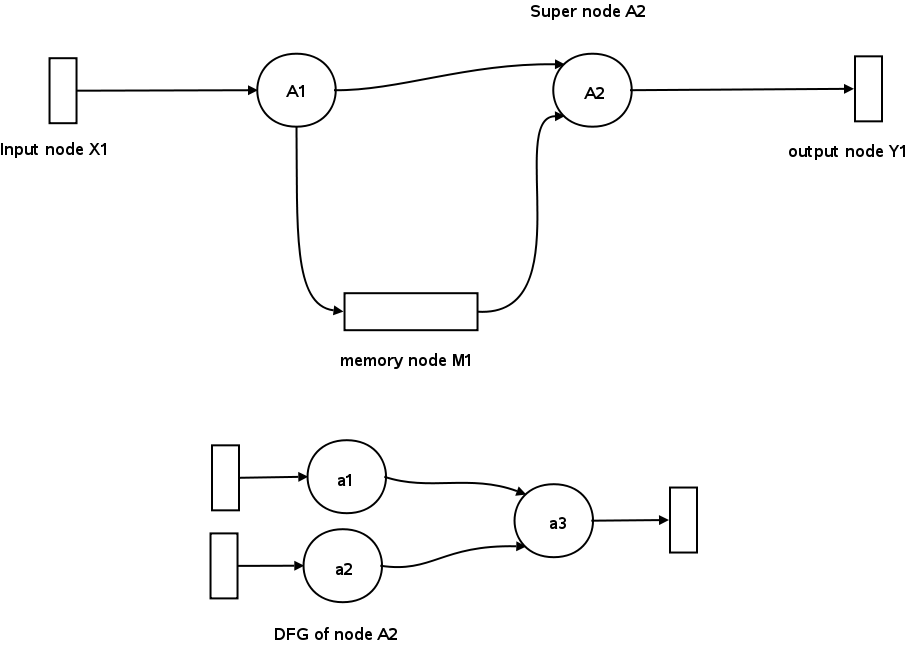
\epsfig{file=figures/Fig_2_11_DFG,width=0.9\textwidth}\\
	  \caption{Flow Graph}
     \end{center}
\end{figure}

\begin{figure}[!hbtp]
     \begin{center}
	  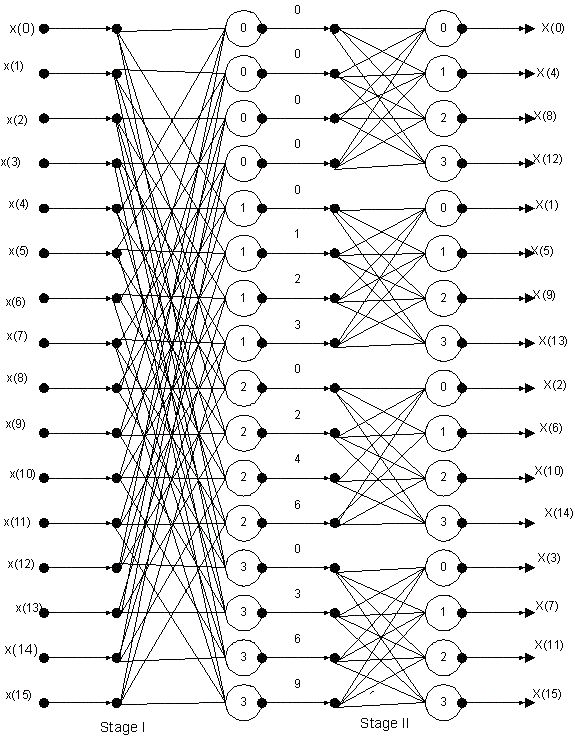
\epsfig{file=figures/Fig_2_12_DFG_FFT,width=0.5\textwidth}\\
	  \caption{DFG of a FFT-algorithm}
     \end{center}
\end{figure}

\os{\newpage}

\bi
	\ite extension of a DFG with control flow \pr \textbf{CFG}
	\ite introduction of ``control''-elements
	\ite edges transfers the control flow
	\ite CFG \pr Flow charts
\ei

\begin{figure}[!hbtp]
     \begin{center}
	  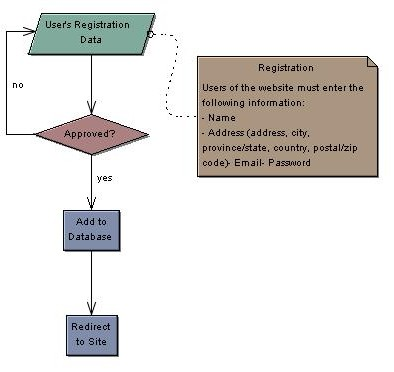
\epsfig{file=figures/Fig_2_13_FlowChart,width=0.7\textwidth}\\
	  \caption{Flow Chart of an Algorithm}
     \end{center}
\end{figure}
\os{\newpage}

\begin{description}
\item[{\rot\bf Message Sequence Charts (MSC) }]~\\[-3ex]
\bigskip
\bi
	\ite modeling of timing and scheduling behaviour
	\ite graphical means for representing schedules
	\bi
		\ite time is a separate axis (timing aspects are explicitly shown)
		\ite time axis vertical
		\ite activity axis horizontal
	\ei

\ei

\begin{figure}[!hbtp]
     \begin{center}
	  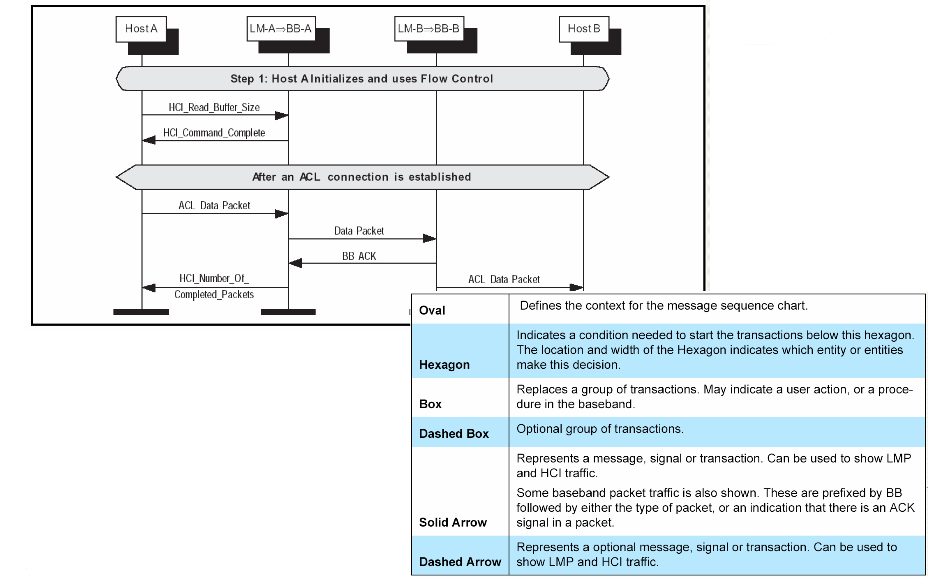
\epsfig{file=figures/Fig_2_14_MSG,width=1.0\textwidth}\\
	  \caption{Message Sequence Chart}
     \end{center}
\end{figure}

\os{\newpage}

\bi
	\ite \textbf{Advantages of activity oriented modeling}
	\bi
		\ite appropriate for visualizing schedules
		\ite proven method for representing schedules in transportation
		\ite hierarchy allowed in DFG and CFG  states.
  	\ei
	\bigskip
	\ite \textbf{Disadvantages}
	\bi
		\ite focused on one case, no timing tolerances or concurreny (MSC)
		\ite no description of non-functional behavior
		\ite no object-orientation
		\ite no description of structural hierarchy (MSC)
	\ei
\ei
\end{description}


%%%%%%%%%%%%%%%%%%%%%%%%%%%%%%%%%%%%%%%%%%%%%%%%%%%%%%%%%%%%%%%%%%%%%%%%%%
\chapter{Cyber-Physical Systems}
%%%%%%%%%%%%%%%%%%%%%%%%%%%%%%%%%%%%%%%%%%%%%%%%%%%%%%%%%%%%%%%%%%%%%%%%%%%
% Chapter: Cyber-Physical Systems
% Examples: examples/cps (Modelica models, the same equations in Python)
%%%%%%%%%%%%%%%%%%%%%%%%%%%%%%%%%%%%%%%%%%%%%%%%%%%%%%%%%%%%%%%%%%%%%%%%%%%

%%%%%%%%%%%%%%%%%%%%%%%%%%%%%%%%%%%%%%%%%%%%%%%%%%%%%%%%%%%%%%%%%%%%%%%%%%%
\section{Overview}
%%%%%%%%%%%%%%%%%%%%%%%%%%%%%%%%%%%%%%%%%%%%%%%%%%%%%%%%%%%%%%%%%%%%%%%%%%%
\nsl{An embedded system never works alone. It measures and influences a
physical process: the temperature of a room, the speed of a motor, the
position of a robot arm. Cyber-physical systems (CPS) are systems in which
this coupling of computation and physics is essential. They are often
distributed and connected, as in a car, a factory, a power grid or an
aircraft. Their behaviour can only be understood if both parts are
described together: the physics with differential equations, the software
with algorithms and state machines.
\newline
Because building and testing the real system is expensive and sometimes
dangerous, CPS are developed with models and simulation. This chapter
introduces the idea of CPS and the steps from a model to the real system.
It then shows how physical systems are modelled with the equation-based
language Modelica, using the free tool OpenModelica, and with a few lines of
Python.
\newpage}

\begin{description}
\item[{\rot\bf What is a cyber-physical system?}]~\\
\defn{def:Cyber-Physical System}
{\textbf{Cyber-physical systems} are integrations of computation with physical processes. Embedded computers and networks monitor and control the physical processes, usually with feedback loops where physical processes affect computations and vice versa. [Edward A.\ Lee, 2008]}
\bi
	\ite combination of mechanical, electrical, thermal, \ldots{} components with software and communication
	\ite examples: driver assistance systems, industrial robots, smart grids, medical devices, building automation
	\ite related terms: \textbf{Internet of Things} (focus on connectivity), \textbf{Industry 4.0} (production), \textbf{digital twin} (a model of a real system that is kept up to date with data from the system)
\ei
\os{\newpage}

\item[{\rot\bf The feedback loop}]~\\[-\lblskip]
\begin{figure}[!hbtp]
\begin{center}
\resizebox{0.85\textwidth}{!}{%
\begin{tikzpicture}[font=\sffamily\small,>=Stealth,
	b/.style={draw,thick,rounded corners,minimum width=30mm,minimum height=12mm,align=center}]
	\node[b,fill=green!15] (proc) at (0,0) {physical process\\(e.g.\ room, motor)};
	\node[b,fill=rwuviolet!15] (sens) at (-4.5,2.2) {sensors\\+ ADC};
	\node[b,fill=rwucyan!10] (comp) at (0,4.4) {computation\\(controller, state machine)};
	\node[b,fill=rwuviolet!15] (act) at (4.5,2.2) {actuators\\+ PWM, DAC};
	\node[b,fill=gray!10] (net) at (6.5,5.6) {network\\other systems};
	\draw[->,thick] (proc) -| node[pos=0.75,left,font=\sffamily\scriptsize]{measured values} (sens);
	\draw[->,thick] (sens) |- (comp);
	\draw[->,thick] (comp) -| (act);
	\draw[->,thick] (act) |- node[pos=0.25,right,font=\sffamily\scriptsize]{forces, heat, \ldots} (proc);
	\draw[<->,thick,dashed] (comp.north east) -- (net);
	\node[font=\sffamily\scriptsize] at (-4.5,4.9) {cyber};
	\node[font=\sffamily\scriptsize] at (-4.5,-0.6) {physical};
	\draw[dashed,gray] (-6.5,1.2) -- (7.5,1.2);
\end{tikzpicture}}
\caption{A cyber-physical system: computation and physical process in a closed loop}
\end{center}
\end{figure}
\bi
	\ite the physical process runs continuously in time; the computer samples and acts at discrete times
	\ite timing is part of the correctness: a controller that reacts too late can make the loop unstable
\ei
\os{\newpage}

\item[{\rot\bf From model to product}]~\\[-\lblskip]
\bi
	\ite the system is developed and tested in steps, replacing models by real parts one after the other
\ei
\begin{figure}[!hbtp]
\begin{center}
\resizebox{0.8\textwidth}{!}{%
\begin{tikzpicture}[font=\sffamily\small,>=Stealth,
	b/.style={draw,thick,rounded corners,minimum height=16mm,text width=30mm,align=center}]
	\node[b,fill=rwucyan!8] (mil) at (0,0) {\textbf{MiL}\\model in the loop\\controller model + plant model};
	\node[b,fill=rwucyan!15] (sil) at (4,0) {\textbf{SiL}\\software in the loop\\real code on the PC + plant model};
	\node[b,fill=rwuviolet!15] (pil) at (8,0) {\textbf{PiL}\\processor in the loop\\code on the target processor};
	\node[b,fill=rwuviolet!25] (hil) at (12,0) {\textbf{HiL}\\hardware in the loop\\real ECU + simulated plant in real time};
	\foreach \a/\b in {mil/sil,sil/pil,pil/hil} \draw[->,thick] (\a) -- (\b);
\end{tikzpicture}}
\caption{Test levels from the model to the real hardware}
\end{center}
\end{figure}
\bi
	\ite \textbf{HiL}: the real control unit runs against a real-time plant simulator -- dangerous or rare situations can be tested safely and repeatably
	\ite our Wokwi simulations are a kind of PiL test: the real firmware on a simulated processor
	\ite \textbf{FMI} 3.0 (2022): standard to exchange models between tools as \textbf{FMU}s for co-simulation
\ei
\os{\newpage}

\item[{\rot\bf Simulation of physical systems}]~\\[-\lblskip]
\bi
	\ite physical systems are described by \textbf{differential equations}, often with algebraic constraints (differential-algebraic equations, DAE)
	\ite models with lumped parameters (masses, springs, resistors) -- ordinary differential equations
	\ite continuous-time physics combined with discrete-time controllers and events (hybrid systems)
	\ite tools
	\bi
		\ite \textbf{block oriented}: MATLAB/Simulink, Xcos (Scilab) -- signals flow in one direction from block to block
		\ite \textbf{equation based} (object oriented): Modelica with OpenModelica (free) or Dymola (commercial) -- components are described by their physical equations
		\ite general programming languages: Python with \texttt{numpy}/\texttt{scipy}, Julia (ModelingToolkit)
	\ei
\ei
\os{\newpage}

\item[{\rot\bf Block oriented modelling}]~\\[-\lblskip]
\bi
	\ite the system is a diagram of blocks with inputs and outputs: gain, sum, integrator, transfer function
	\ite every connection has a fixed direction (causality): the modeller decides what is computed from what
\ei
\begin{figure}[!hbtp]
\begin{center}
\resizebox{0.6\textwidth}{!}{%
\begin{tikzpicture}[font=\sffamily\small,>=Stealth,
	b/.style={draw,thick,minimum width=14mm,minimum height=10mm}]
	\node[b] (gain) at (0,0) {$-a$};
	\node[b] (int) at (3,0) {$\displaystyle\int dt$};
	\draw[->,thick] (gain) -- node[above]{$\dot x$} (int);
	\draw[->,thick] (int) -- (5,0) node[right]{$x$};
	\draw[->,thick] (4.3,0) |- (1.5,-1.4) -| ($(gain.west)+(-0.6,0)$) -- (gain.west);
	\fill (4.3,0) circle (1.5pt);
	\node[below,font=\sffamily\scriptsize] at (3,0.9) {$x(0)=1$};
\end{tikzpicture}}
\caption{Block diagram of $\dot x = -a\,x$: the output of the integrator is fed back}
\end{center}
\end{figure}
\bi
	\ite natural for control engineering and signal processing
	\ite for physical networks (electrical circuits, mechanics) the modeller must first solve the equations for the right variables by hand -- this is what equation-based tools avoid
\ei
\os{\newpage}
\end{description}

%%%%%%%%%%%%%%%%%%%%%%%%%%%%%%%%%%%%%%%%%%%%%%%%%%%%%%%%%%%%%%%%%%%%%%%%%%%
\section{Modelling with Modelica}
%%%%%%%%%%%%%%%%%%%%%%%%%%%%%%%%%%%%%%%%%%%%%%%%%%%%%%%%%%%%%%%%%%%%%%%%%%%
\nsl{Modelica is a language for describing physical systems by equations. A
model states which relations hold, for example Ohm's law $u = R \cdot i$,
without saying which variable is computed from which. The compiler sorts the
equations, solves them symbolically where possible and generates simulation
code. Components can be connected like real parts: connecting a resistor to
a capacitor automatically produces Kirchhoff's laws. Modelica is
standardised by the Modelica Association. OpenModelica is a free
implementation with a graphical editor (OMEdit) and an extensive standard
library for electrical, mechanical, thermal, fluid and control components.}

\begin{description}
\item[{\rot\bf Features of Modelica / OpenModelica}]~\\[-\lblskip]
\bi
	\ite \textbf{equation based} (acausal): equations instead of assignments -- the tool decides the order of computation
	\ite \textbf{object oriented}: classes, instances, inheritance, packages; parameters separate from the structure (a resistor model, used with different values)
	\ite \textbf{multi-domain}: electrical, mechanical, thermal, hydraulic, \ldots{} components in one model
	\ite \textbf{connectors} with potential variables (voltage, temperature) and flow variables (current, heat flow): \texttt{connect()} creates the equations ``potentials equal, sum of flows zero''
	\ite physical units for all quantities (\texttt{unit = "V"}) -- the tool checks them
	\ite graphical (drag and drop in OMEdit) and textual modelling of the same model
	\ite export as FMU for co-simulation; code generation for controllers
\ei
\os{\newpage}

\item[{\rot\bf OpenModelica: graphical modelling}]~\\[-\lblskip]
\begin{figure}[!hbtp]%
     \begin{center}
	  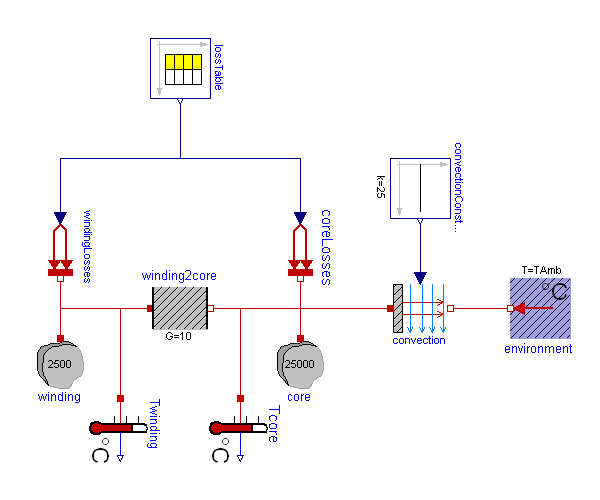
\epsfig{file=figures/Fig_3_3_OpenModelica,width=0.8\textwidth}\\
	  \caption{OpenModelica model of a heat transfer}
     \end{center}
\end{figure}
\os{\newpage}

\item[{\rot\bf First elements of Modelica}]~\\[-\lblskip]
\bi
	\ite data types: \texttt{Real} (64 bit floating point), \texttt{Integer}, \texttt{Boolean}, \texttt{String}, enumerations
	\ite \texttt{parameter}: constant during a simulation, can be changed between simulations
	\ite \texttt{der(x)}: time derivative $\dot x$
	\ite \texttt{start}: initial value; \texttt{fixed = true}: the initial value must hold exactly
	\ite example: $\dot x = -a \cdot x$
\ei
\begin{lstlisting}[language={}]
model HDE
  Real x(start = 1, fixed = true);
  parameter Real a = 1;
equation
  der(x) = -a*x;
end HDE;
\end{lstlisting}
\os{\newpage}

\begin{figure}[!hbtp]
     \begin{center}
	  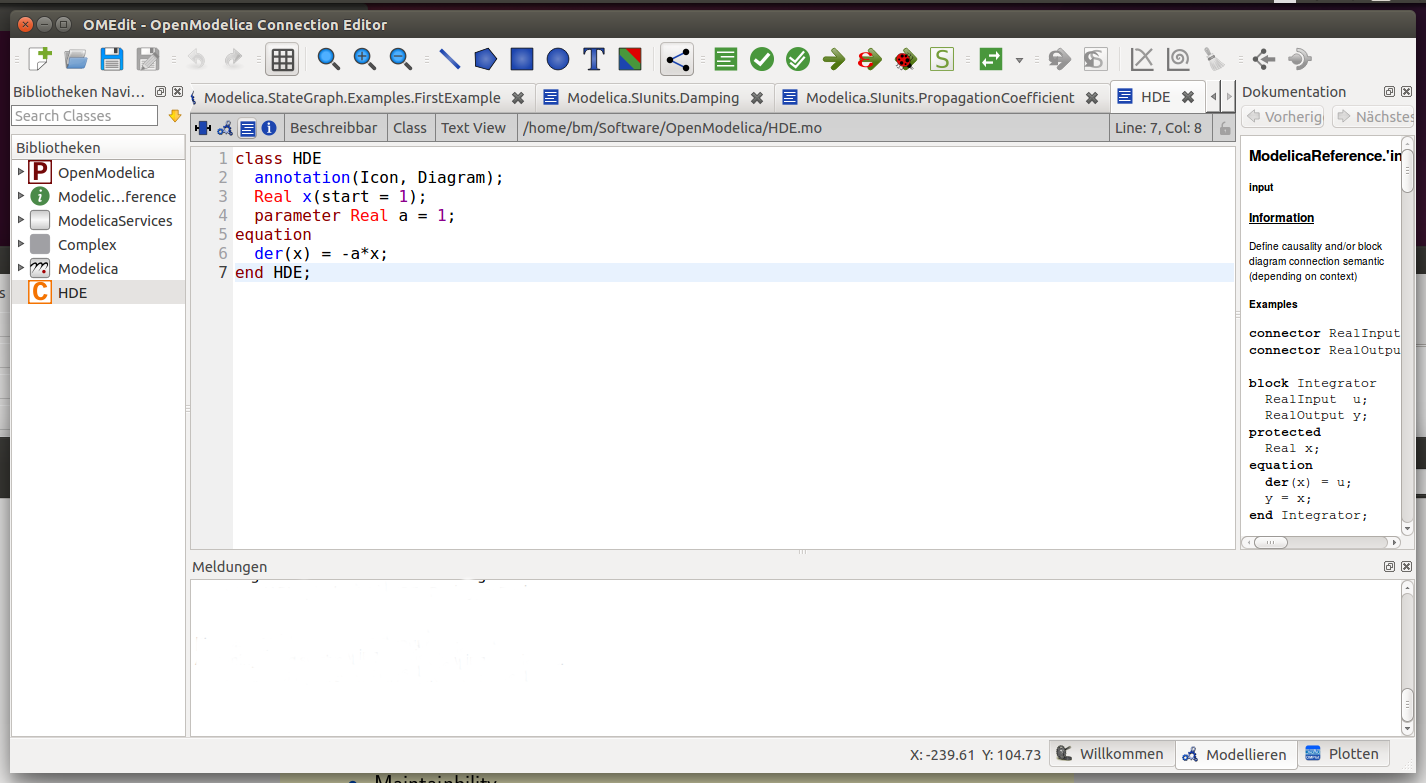
\epsfig{file=figures/Fig_3_4_HDE_OMEdit,width=0.75\textwidth}\\
	  \caption{Model HDE in OMEdit}
     \end{center}
\end{figure}
\os{\newpage}

\begin{figure}[!hbtp]
     \begin{center}
	  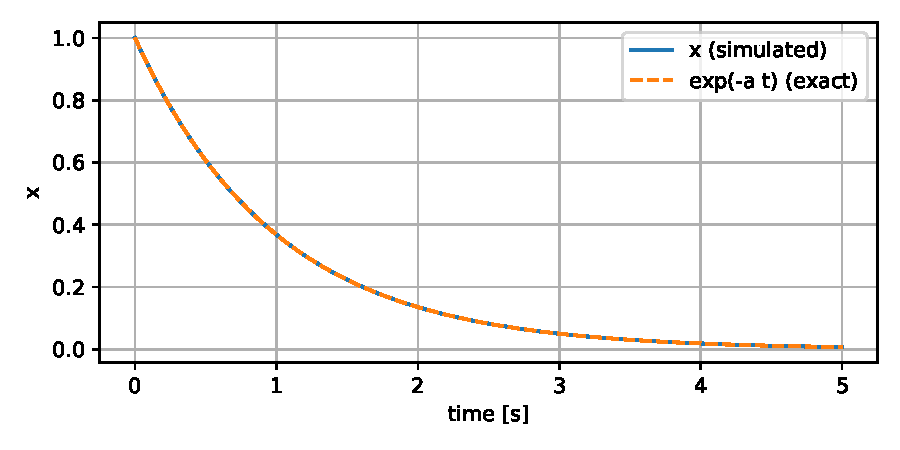
\epsfig{file=figures/cps_hde.pdf,width=0.75\textwidth}\\
	  \caption{Solution of the model HDE: simulation and exact solution $x(t) = e^{-a t}$}
     \end{center}
\end{figure}
\os{\newpage}

\item[{\rot\bf Differential-algebraic equations: the pendulum}]~\\[-\lblskip]
\bi
	\ite a model can contain algebraic equations (without derivatives) besides the differential equations
	\ite example: a planar pendulum, a mass $m$ on a rod of length $L$; the rod force $F$ is unknown
\ei
\begin{minipage}{0.3\textwidth}
\begin{center}
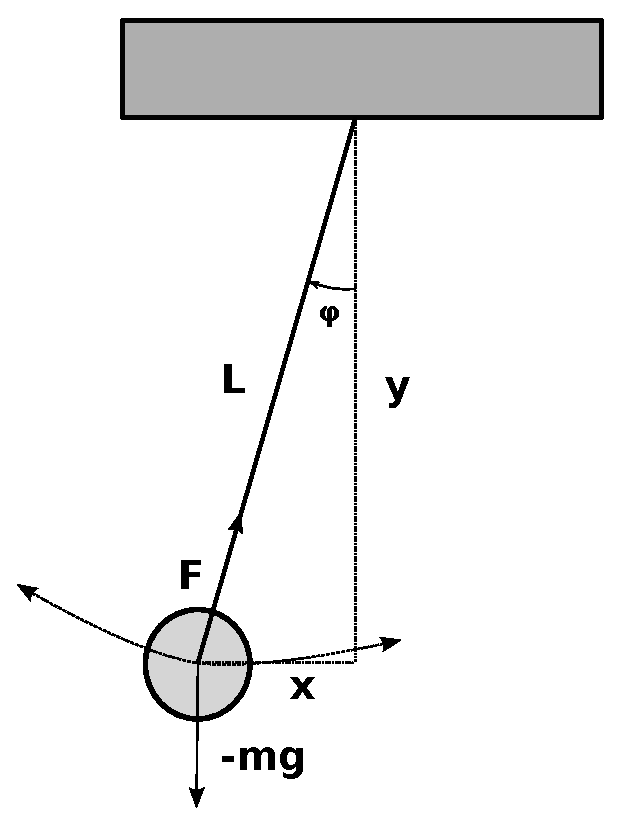
\epsfig{file=figures/Fig_3_6_Pendulum,width=0.8\textwidth}
\end{center}
\end{minipage}
\begin{minipage}{0.65\textwidth}
\begin{eqnarray*}
m\,\dot{v}_x &=& -\frac{x}{L}\,F \\
m\,\dot{v}_y &=& -\frac{y}{L}\,F - m\,g \\
\dot{x} &=& v_x \\
\dot{y} &=& v_y \\
x^2 + y^2 &=& L^2
\end{eqnarray*}
\end{minipage}
\bi
	\ite 5 equations for 5 unknowns ($x, y, v_x, v_y, F$); the last equation is the constraint of the rod
\ei
\os{\newpage}

\item[{\rot\bf The pendulum in Modelica}]~\\[-\lstskip]
\begin{lstlisting}[language={}]
model Pendulum "Planar pendulum"
  parameter Real m = 1, g = 9.81, L = 0.5;
  Real F;
  Real x(start = 0.5, fixed = true), y(start = 0);
  Real vx, vy;
equation
  m*der(vx) = -(x/L)*F;
  m*der(vy) = -(y/L)*F - m*g;
  der(x) = vx;
  der(y) = vy;
  x^2 + y^2 = L^2;   // algebraic equation (constraint of the rod)
end Pendulum;
\end{lstlisting}
\bi
	\ite the equations are written as in the physics book; OpenModelica reduces the DAE (index reduction) and chooses the state variables itself
\ei
\os{\newpage}

\begin{figure}[!hbtp]
     \begin{center}
	  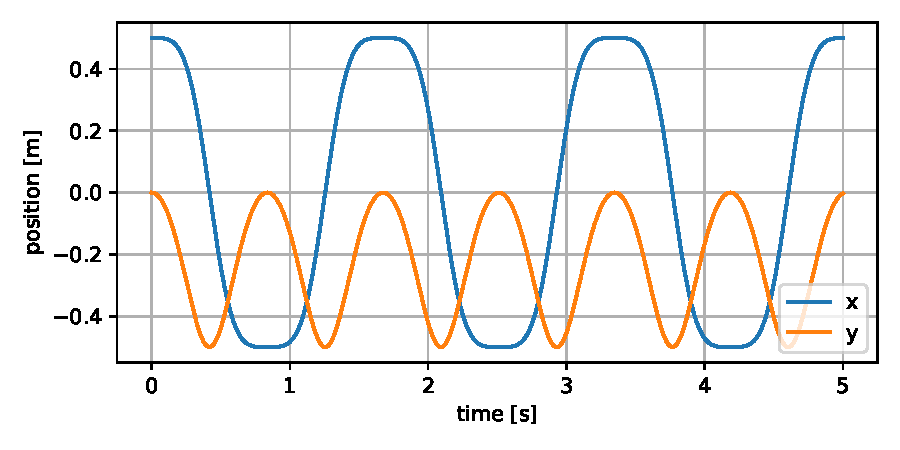
\epsfig{file=figures/cps_pendulum.pdf,width=0.8\textwidth}\\
	  \caption{Horizontal and vertical position of the pendulum, started with the rod horizontal}
     \end{center}
\end{figure}
\bi
	\ite $y$ is always $\le 0$: the mass swings below the pivot; the period is longer than for small angles
\ei
\os{\newpage}

\item[{\rot\bf Classes and instances}]~\\[-\lblskip]
\bi
	\ite every object has a class that defines its data and its behaviour
	\ite a class has variables (constants, parameters, computed values), equations, and can contain instances of other classes
\ei
\begin{lstlisting}[language={}]
class Point "Point in a three-dimensional space"
  Real x;
  Real y;
  Real z;
end Point;

class Triangle
  Point point1;
  Point point2;
  Point point3;
end Triangle;

class Triangle2 "with modification of an instance"
  Point point1(x = 1, y = 2, z = 3);
  Point point2;
  Point point3;
end Triangle2;
\end{lstlisting}
\os{\newpage}

\item[{\rot\bf An electrical example}]~\\[-\lblskip]
\begin{minipage}{0.35\textwidth}
\begin{center}
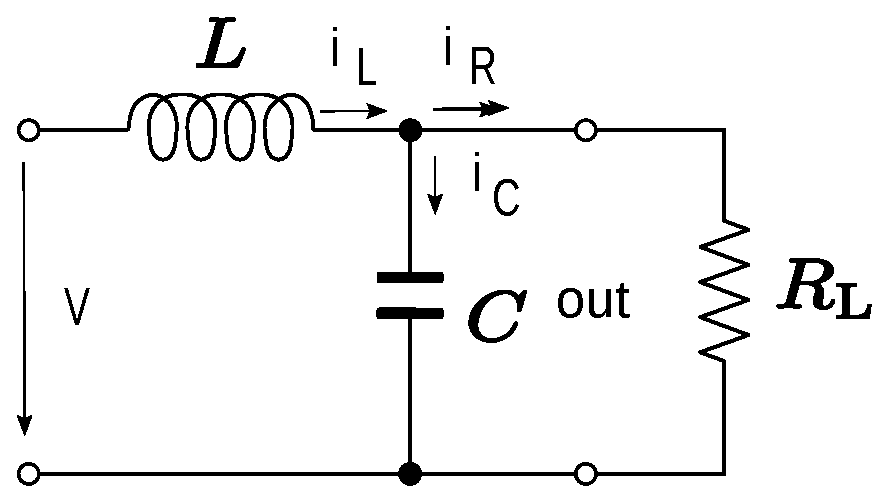
\epsfig{file=figures/Fig_3_8_RLC,width=0.9\textwidth}
\end{center}
\end{minipage}
\begin{minipage}{0.6\textwidth}
\begin{lstlisting}[language={}]
model RLC1 "A resistor-inductor-capacitor circuit"
  type Voltage = Real(unit = "V");
  type Current = Real(unit = "A");
  parameter Voltage Vb = 24 "Battery voltage";
  parameter Real L(unit = "H") = 1;
  parameter Real R(unit = "Ohm") = 100;
  parameter Real C(unit = "F") = 1e-3;
  Voltage V;
  Current i_L, i_R, i_C;
equation
  V = i_R*R;
  C*der(V) = i_C;
  L*der(i_L) = Vb - V;
  i_L = i_R + i_C;
end RLC1;
\end{lstlisting}
\end{minipage}
\os{\newpage}

\begin{figure}[!hbtp]
     \begin{center}
	  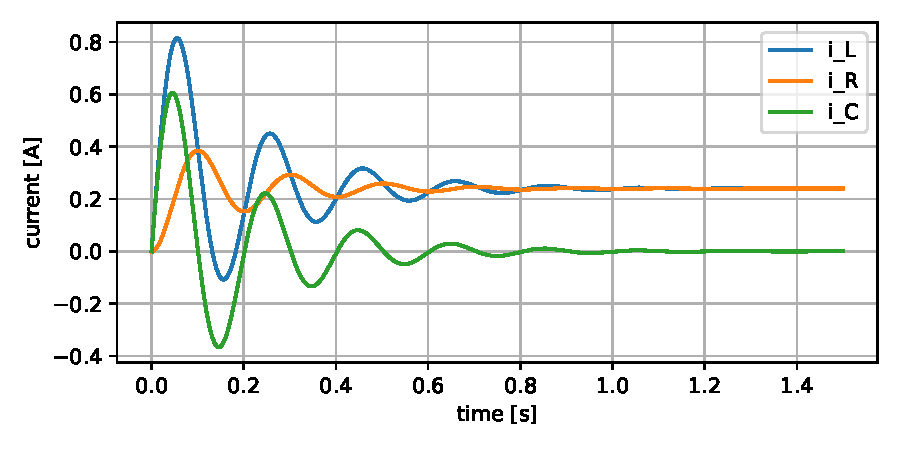
\epsfig{file=figures/cps_rlc.pdf,width=0.8\textwidth}\\
	  \caption{Currents in the RLC circuit after switching on the battery}
     \end{center}
\end{figure}
\bi
	\ite damped oscillation ($\omega_0 = 1/\sqrt{LC} \approx 31.6$\,s$^{-1}$, i.e.\ about 5\,Hz); final state $i_L = i_R = V_b/R = 0.24$\,A, $i_C = 0$
\ei
\os{\newpage}

\item[{\rot\bf The same equations in Python}]~\\[-\lstskip]
\begin{lstlisting}[language=Python]
from scipy.integrate import solve_ivp

Vb, L, R, C = 24.0, 1.0, 100.0, 1e-3

def rlc(t, s):            # state: capacitor voltage V, inductor current i_L
    V, iL = s
    return [(iL - V / R) / C,      # C dV/dt   = i_C = i_L - V/R
            (Vb - V) / L]          # L di_L/dt = Vb - V

sol = solve_ivp(rlc, (0, 1.5), [0.0, 0.0], max_step=1e-3)
print("final i_L =", sol.y[1][-1])   # 0.240 A
\end{lstlisting}
\bi
	\ite here the equations had to be solved for the derivatives by hand -- for the RLC circuit easy, for the pendulum DAE not (we used the angle as the only state)
	\ite this is exactly the work Modelica does automatically for large models
	\ite the plots of this chapter were created with this script (\texttt{examples/cps/simulate.py}, runs on Replit)
\ei
\os{\newpage}

\item[{\rot\bf Exercises}]~\\[-\lblskip]
\bi
	\ite Simulate \texttt{HDE}, \texttt{Pendulum} and \texttt{RLC1} in OpenModelica and compare with the plots of the Python script.
	\ite Change $R$ in the RLC circuit to $10\,\Omega$ and $1000\,\Omega$. When does the circuit stop oscillating? Compare with the condition $R = \frac{1}{2}\sqrt{L/C}$.
	\ite Build the RLC circuit graphically from the Modelica standard library (\texttt{Modelica.Electrical.Analog}) and compare the generated equations with \texttt{RLC1}.
	\ite Add a two-point controller to a heated room model: heating on below 20\,$^\circ$C, off above 21\,$^\circ$C. How does the hysteresis influence the switching frequency?
\ei
\end{description}


%%%%%%%%%%%%%%%%%%%%%%%%%%%%%%%%%%%%%%%%%%%%%%%%%%%%%%%%%%%%%%%%%%%%%%%%%%
\chapter{Processors}
%%%%%%%%%%%%%%%%%%%%%%%%%%%%%%%%%%%%%%%%%%%%%%%%%%%%%%%%%%%%%%%%%%%%%%%%%%%
\section{Processors for Embedded Systems}
%%%%%%%%%%%%%%%%%%%%%%%%%%%%%%%%%%%%%%%%%%%%%%%%%%%%%%%%%%%%%%%%%%%%%%%%%%%
\nsl{Embedded systems need special processors. A standard PC processor isn't suitable, as the microprocessor used doesn't operate independently. It has to be implanted on a motherboard, which serves as the communication interface between the processor and other input/output devices. This involves increased costs and such a system occupies a large space.
\newline
Shifting our focus to microcontrollers, we observe that an 8-bit microcontroller possesses small computing power and has too many restrictions in building an appropriate internal or external memory. So these types of processors are also not suitable for a sophisticated embedded system. The above mentioned restrictions are not evident when working with 16- and 32-bit microcontrollers. A big advantage of these types of microcontrollers is that nearly every type of interface is available which we might have to use in an embedded system.
\newline
If an Embedded application/project allows us to use a small motherboard (no hard discs and usually no GUI 'graphical user interfaces' etc.) then it makes sense to deploy an ``Embedded PC'' or a PC/104 system. Such systems contain a special, so called ``Mobile microprocessor'' like ``Pentium M'' or ``Geode'' or ``XScale''. These processors are variants of standard 8086-type microprocessors (Pentium M and Geode). If we are working with these Embedded PC's, then you have access to support in the form of well known standard PC tools like compilers, linkers and operating systems. 
\newline
Another type of processor which could be present in an embedded system is a signal processor. A signal processor has much more computing power than a microcontroller. But on the contrary to a microprocessor, a signal processor has nearly the same interfaces available in a microcontroller. The disadvantage of using a signal processor is that there aren't much development tools available.
}

\begin{description}
\bigskip
\item[{\rot\bf Microprocessors for Embedded Systems }]~\\[-3ex]
\bi
	\ite use a special version of an 8086-type of microprocessors (Pentium M or Geode)
	\ite these microprocessor are integrated in an ``embedded PC'' or a ``PC/104-system''
	\ite these type of PCs' work without any hard disc (and without any cooling system)
	\ite instead of a hard disc, a ``FLASH Memory'' is used (e.g. SD-Card)
	\ite if a graphical user interface is available, then the ``graphical processing unit'' is a part of the microprocessor.
\ei
\os{\newpage}
\begin{figure}[!hbtp]
     \begin{center}
	  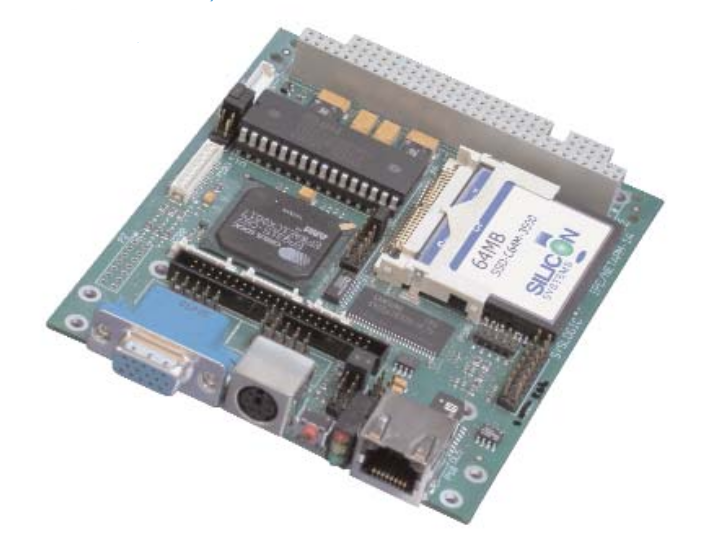
\epsfig{file=figures/Fig_3_1_SBC,width=0.7\textwidth}\\
	  \caption{Embedded PC as Single Board Computer}
     \end{center}
\end{figure}
\os{\newpage}     

\begin{figure}[!hbtp]
     \begin{center}
	  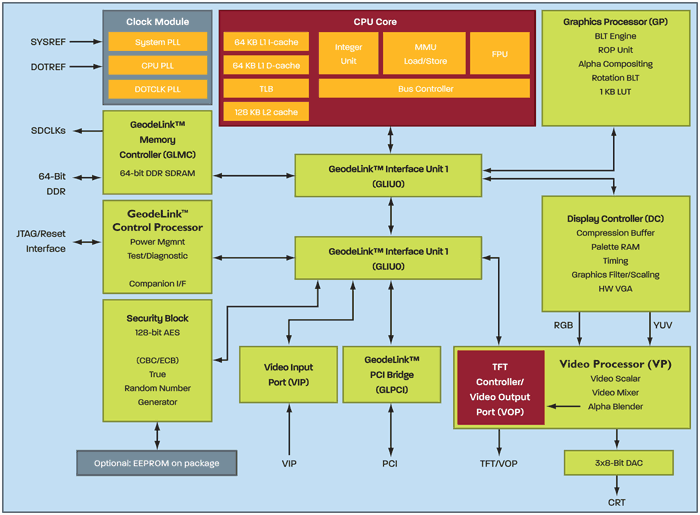
\epsfig{file=figures/Fig_3_2_Blockdiagram_Geode,width=0.8\textwidth}\\
	  \caption{Blockdiagram of a Geode-Microprocessor}
     \end{center}
\end{figure}
\os{\newpage}    

\begin{figure}[!hbtp]
     \begin{center}
	  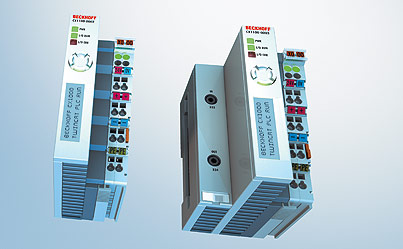
\epsfig{file=figures/Fig_3_3_Embedded_PC,width=0.9\textwidth}\\
	  \caption{A different type of Embedded PC}
     \end{center}
\end{figure} 
\os{\newpage}

\item[{\rot\bf Signal processors for Embedded Systems }]~\\[-3ex]
\os{\bigskip}
\bi
	\ite same structure as microcontrollers
	\bi 
		\ite a lot of interfaces
		\ite external memory available as instruction and data memory (Harvard architecture)
		\ite building of programs using cross-development technique
	\ei
	\bigskip
	\ite much higher computing power than microcontrollers 
	\ite specially built for signal processing applications (e.g. video compression, audio processing etc.)  
\ei
\os{\newpage}

\begin{figure}[!hbtp]
     \begin{center}
	  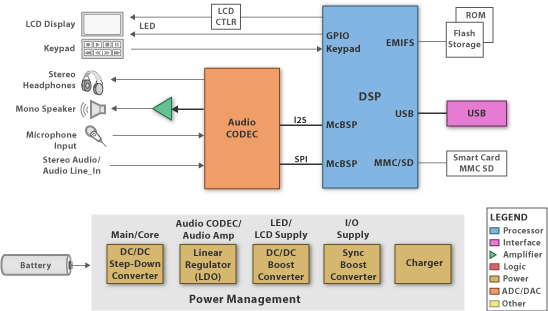
\epsfig{file=figures/Fig_3_4_DSP_MP3,width=0.9\textwidth}\\
	  \caption{MP3-Player, an Application for DSP-Processors}
     \end{center}
\end{figure}
\os{\newpage}

\item[{\rot\bf Microcontrollers for Embedded Systems }]~\\[-3ex]
\os{\bigskip}
\bi
	\ite most embedded systems employ a microcontroller
	\ite differences in the use of internal memory and/or external memory
	\ite human interface almost nonexistent or really small
	\bigskip 
	\ite according to the reduction of hardware costs more functions imlemented in a processor
	\ite a combination of microcontroller and signal processor are build (OMAP-Processor, part of the Beagle-Board)
	
\ei
\os{\newpage}

\begin{figure}[!hbtp]
     \begin{center}
	  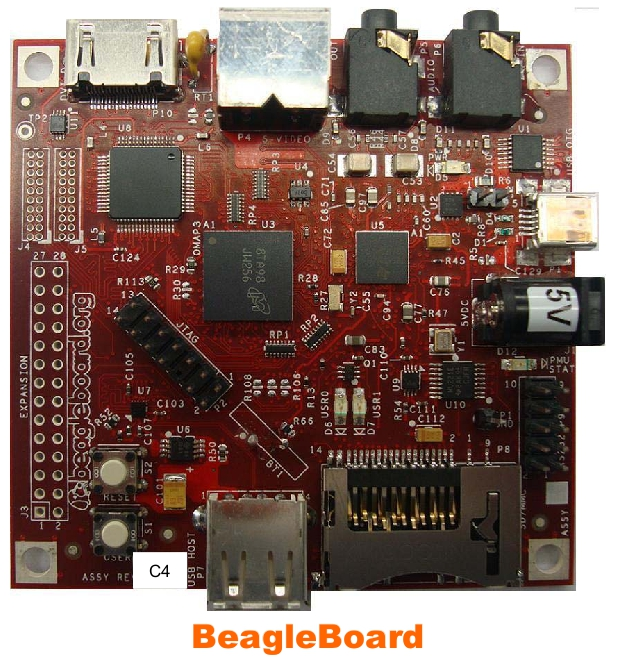
\epsfig{file=figures/Fig_3_5_BeagleBoard,width=0.5\textwidth}\\
	  \caption{Beagle Board with OMAP-Processor}
     \end{center}
\end{figure}
\os{\newpage}     

\item[{\rot\bf Components of the microcontroller/signal processor based Beagle Board }]~\\[-3ex]
\os{\bigskip}
\bi
	\ite microcontroller ARM Cortex-A8 (wordlength 32 Bit)
	\ite signalprocessor TMS 320DM641 (fix point digital signal processor, wordlenth 32 bit, multi media control and interfaces) 
	\ite TPS 65950 Reset and Power Management
	\ite TFP 410 Interface to external LCD panels
	\ite different digital interfaces (I/0)
	
\ei
\os{\newpage}

\begin{figure}[!hbtp]
     \begin{center}
	  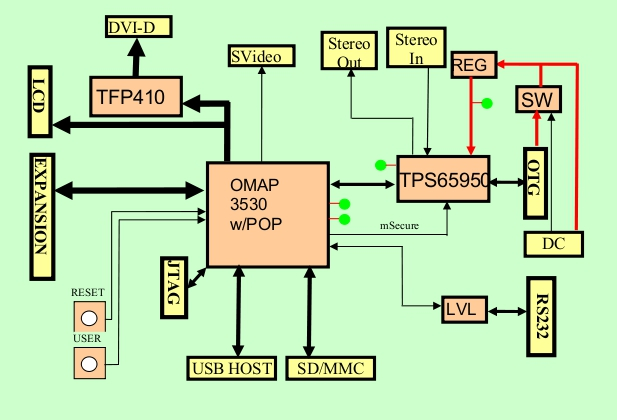
\epsfig{file=figures/Fig_3_6_ProcessorsBeagleBoard,width=0.8\textwidth}\\
	  \caption{Blockdiagram of a Beagle Board with different Processors}
     \end{center}
\end{figure}
\os{\newpage}

\begin{figure}[!hbtp]
     \begin{center}
	  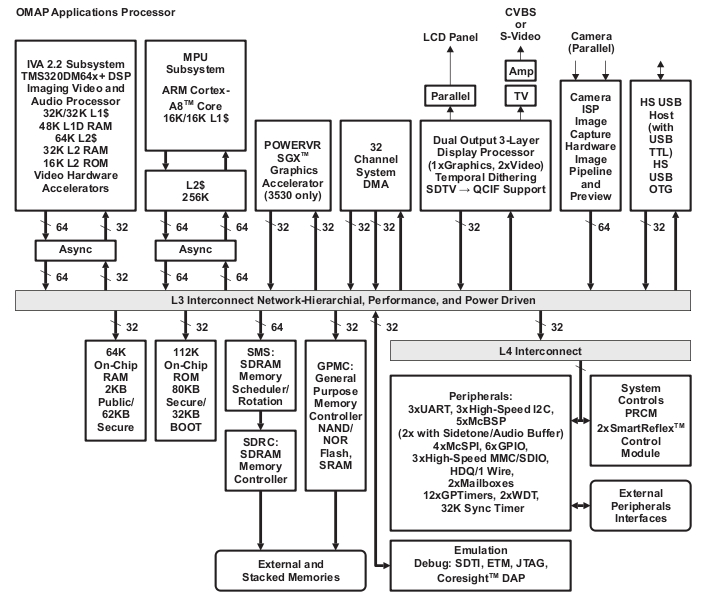
\epsfig{file=figures/Fig_3_7_InternalOMAP,width=0.7\textwidth}\\
	  \caption{Features of a OMAP-Processor}
     \end{center}
\end{figure}
\os{\newpage}     
\end{description}

%%%%%%%%%%%%%%%%%%%%%%%%%%%%%%%%%%%%%%%%%%%%%%%%%%%%%%%%%%%%%%%%%%%%%%%%%%%
\section{Overview about ARM Processors}
%%%%%%%%%%%%%%%%%%%%%%%%%%%%%%%%%%%%%%%%%%%%%%%%%%%%%%%%%%%%%%%%%%%%%%%%%%%
\begin{description}
\bigskip
\item[{\rot\bf Background }]~\\[-3ex]
\bi
	\ite ARM-Processors mostly part of a SoC (System on chip)
	\ite ARM-Processor itself is a IP-Core (intellectual property core), means a lisenced part which contains the processor funtionality
	\ite ARM-IP-Cores placed in a lot of different boards (like smart phones, embedded systems) and in the beagle bord  
	\bi 
		\ite same register model for address- and data register.
		\ite implementation of a 'load/store' architecture
		\ite use super user- and a user mode. (Priority of execution)
	\ei
	\ite implementation of superscalar architecture (Processing unit focused on integer processing).
	\ite integration of FPU coprocessor (NEON Processing unit focused on Floating Point processing). 
	\ite in some processors a MMU (\underline{m}emory \underline{m}anagement \underline{u}nit) is implemented (important for operation systems)
	\ite supports SIMD-applications.
	\ite integration of a lot of interfaces 
\ei

\os{\newpage}

\begin{figure}[!hbtp]
     \begin{center}
	  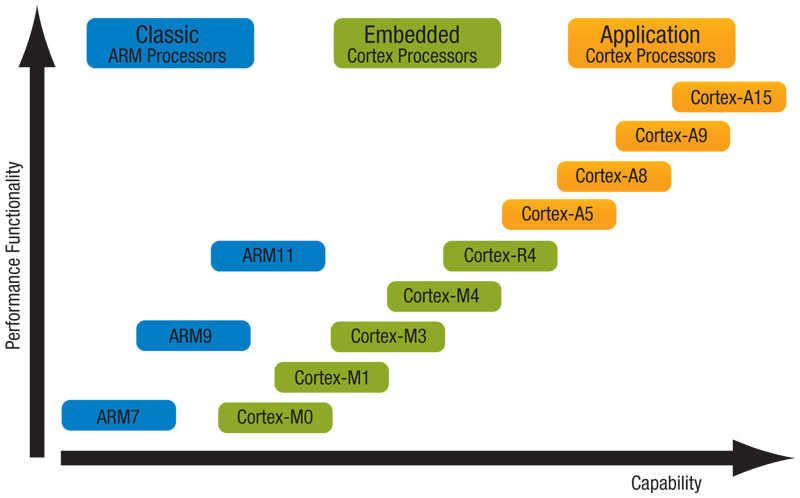
\epsfig{file=figures/Fig_3_8_ARMProcessors,width=0.85\textwidth}\\
	  \caption{Overview about different ARM-Processors}
     \end{center}
\end{figure}
\os{\newpage}
\end{description}



%%%%%%%%%%%%%%%%%%%%%%%%%%%%%%%%%%%%%%%%%%%%%%%%%%%%%%%%%%%%%%%%%%%%%%%%%%%
\section{Functions of the ARM-Cortex-A8-Processor}
%%%%%%%%%%%%%%%%%%%%%%%%%%%%%%%%%%%%%%%%%%%%%%%%%%%%%%%%%%%%%%%%%%%%%%%%%%%
\begin{description}
\item[{\rot\bf General Functions }]~\\[-3ex]
\bigskip
\bi
	\ite ARM-architecture is a RISC-architecture (\underline{r}educed \underline{i}nstruction \underline{s}et \underline{c}omputer)
	\ite according to the RISC-architecture more register banks are available (for every processor unit)
	\ite wordlength of the integer unit (and address unit) 32 Bit (wordlength of general purpose register 32 bit)
	\ite implements a superscalar architecture 
	\ite internal Harvard architecture based on two different caches- Instruction and Data (I-Cache and D-Cache respectively).
	\ite memory management unit (MMU).
	\ite different instruction set for: 
	\bi 
		\ite Thumb-instruction set (16 bit integer unit)
		\ite ARM-instruction set (32 bit integer unit)
		\ite ThumbEE-instruction set (32 bit integer unit without MMU)
		\ite NEON-, VFP-instruction set (for SIMD applications in integer (NEON) or floating point format (VFP)
		\ite FP-instruction set (for single floating point numbers) 
	\ei
\ei

\os{\newpage}
\begin{figure}[!hbtp]
     \begin{center}
	  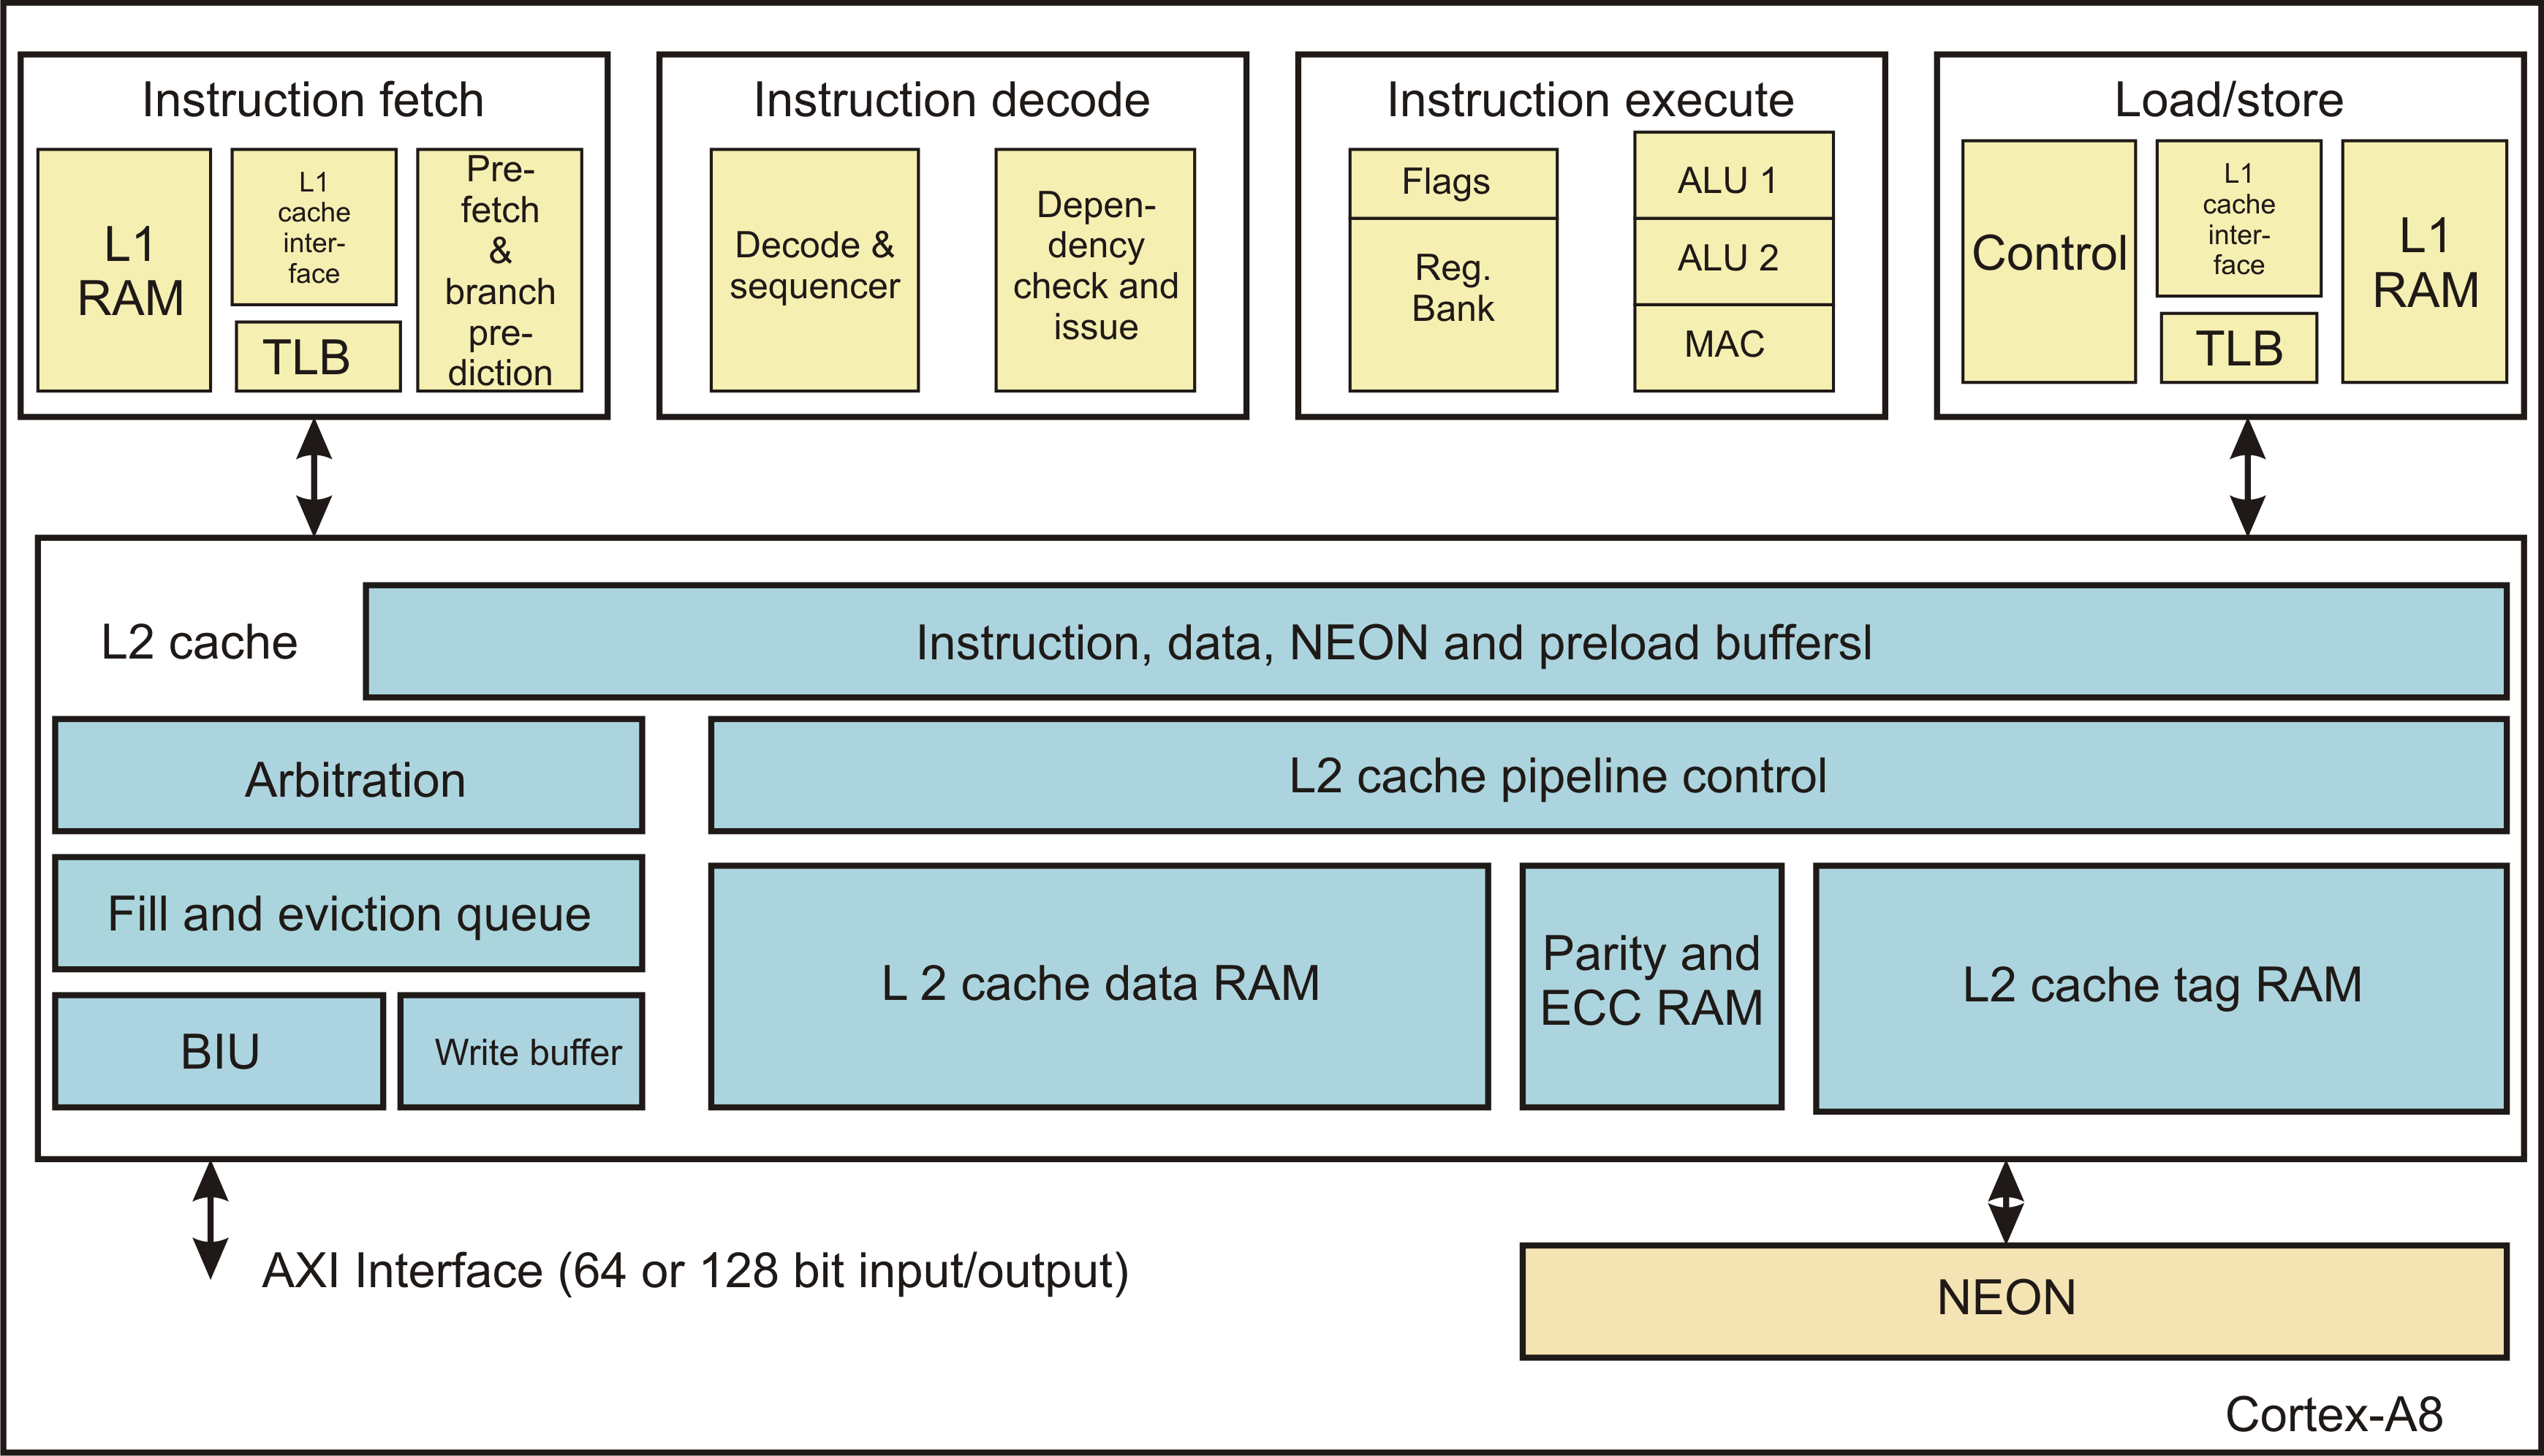
\epsfig{file=figures/Fig_3_9_Cortex.png,width=0.95\textwidth}\\
	  \caption{Blockdiagram Cortex-A8-Processor}
     \end{center}
\end{figure}     
\os{\newpage}

\item[{\rot\bf ALU1,2 }]~\\[-3ex]

\bi 
	\ite both ALU (ALU1 and ALU2) contains 32-bit integer units (could be used for signed, unsigned and fix point operations).
	\ite standard wordlength 32 bit
	\bi 
		\ite word 32 bit (data manipulation, address operations)
		\ite halfword 16 bit (data) 
		\ite byte 8 bit (data)
		\bigskip
		\ite doubleword 64 bit (data)
	\ei
	\bigskip 
	\ite works with RISC-operation on fixed length instructions (32 bit).
	\bi
		\ite load/store technique used
		\ite in every instruction a register is involved (as a source or destination register)
		\ite the order of operands are allways the same 
		\ite special data transfer instruction implemented for a read access (load) and a write access (store)
		\ite function calls work register based (not memory based as for CISC-processors)
		\ite conditions could be used for transfer and data manipulation instructions
	\ei
	\ite pipeline not visible for the user (only in some special instructions an insert of NOPs are necessary to synchronize the pipeline).
	\ite to support the pipeline operation for branches (especially conditional branches) a branch cache is involved.
	\ite three different instruction sets are available for the ALU
	\bi
		\ite Thumb instruction set for 16 bit applications
		\ite ThumbEE instruction set for 32 bit applications (typical embedded applications)
		\ite ARM instruction set for 32 bit application and the support of virtual memory management systems
	\ei
\ei
\os{\newpage}
\begin{figure}[!hbtp]
     \begin{center}
	  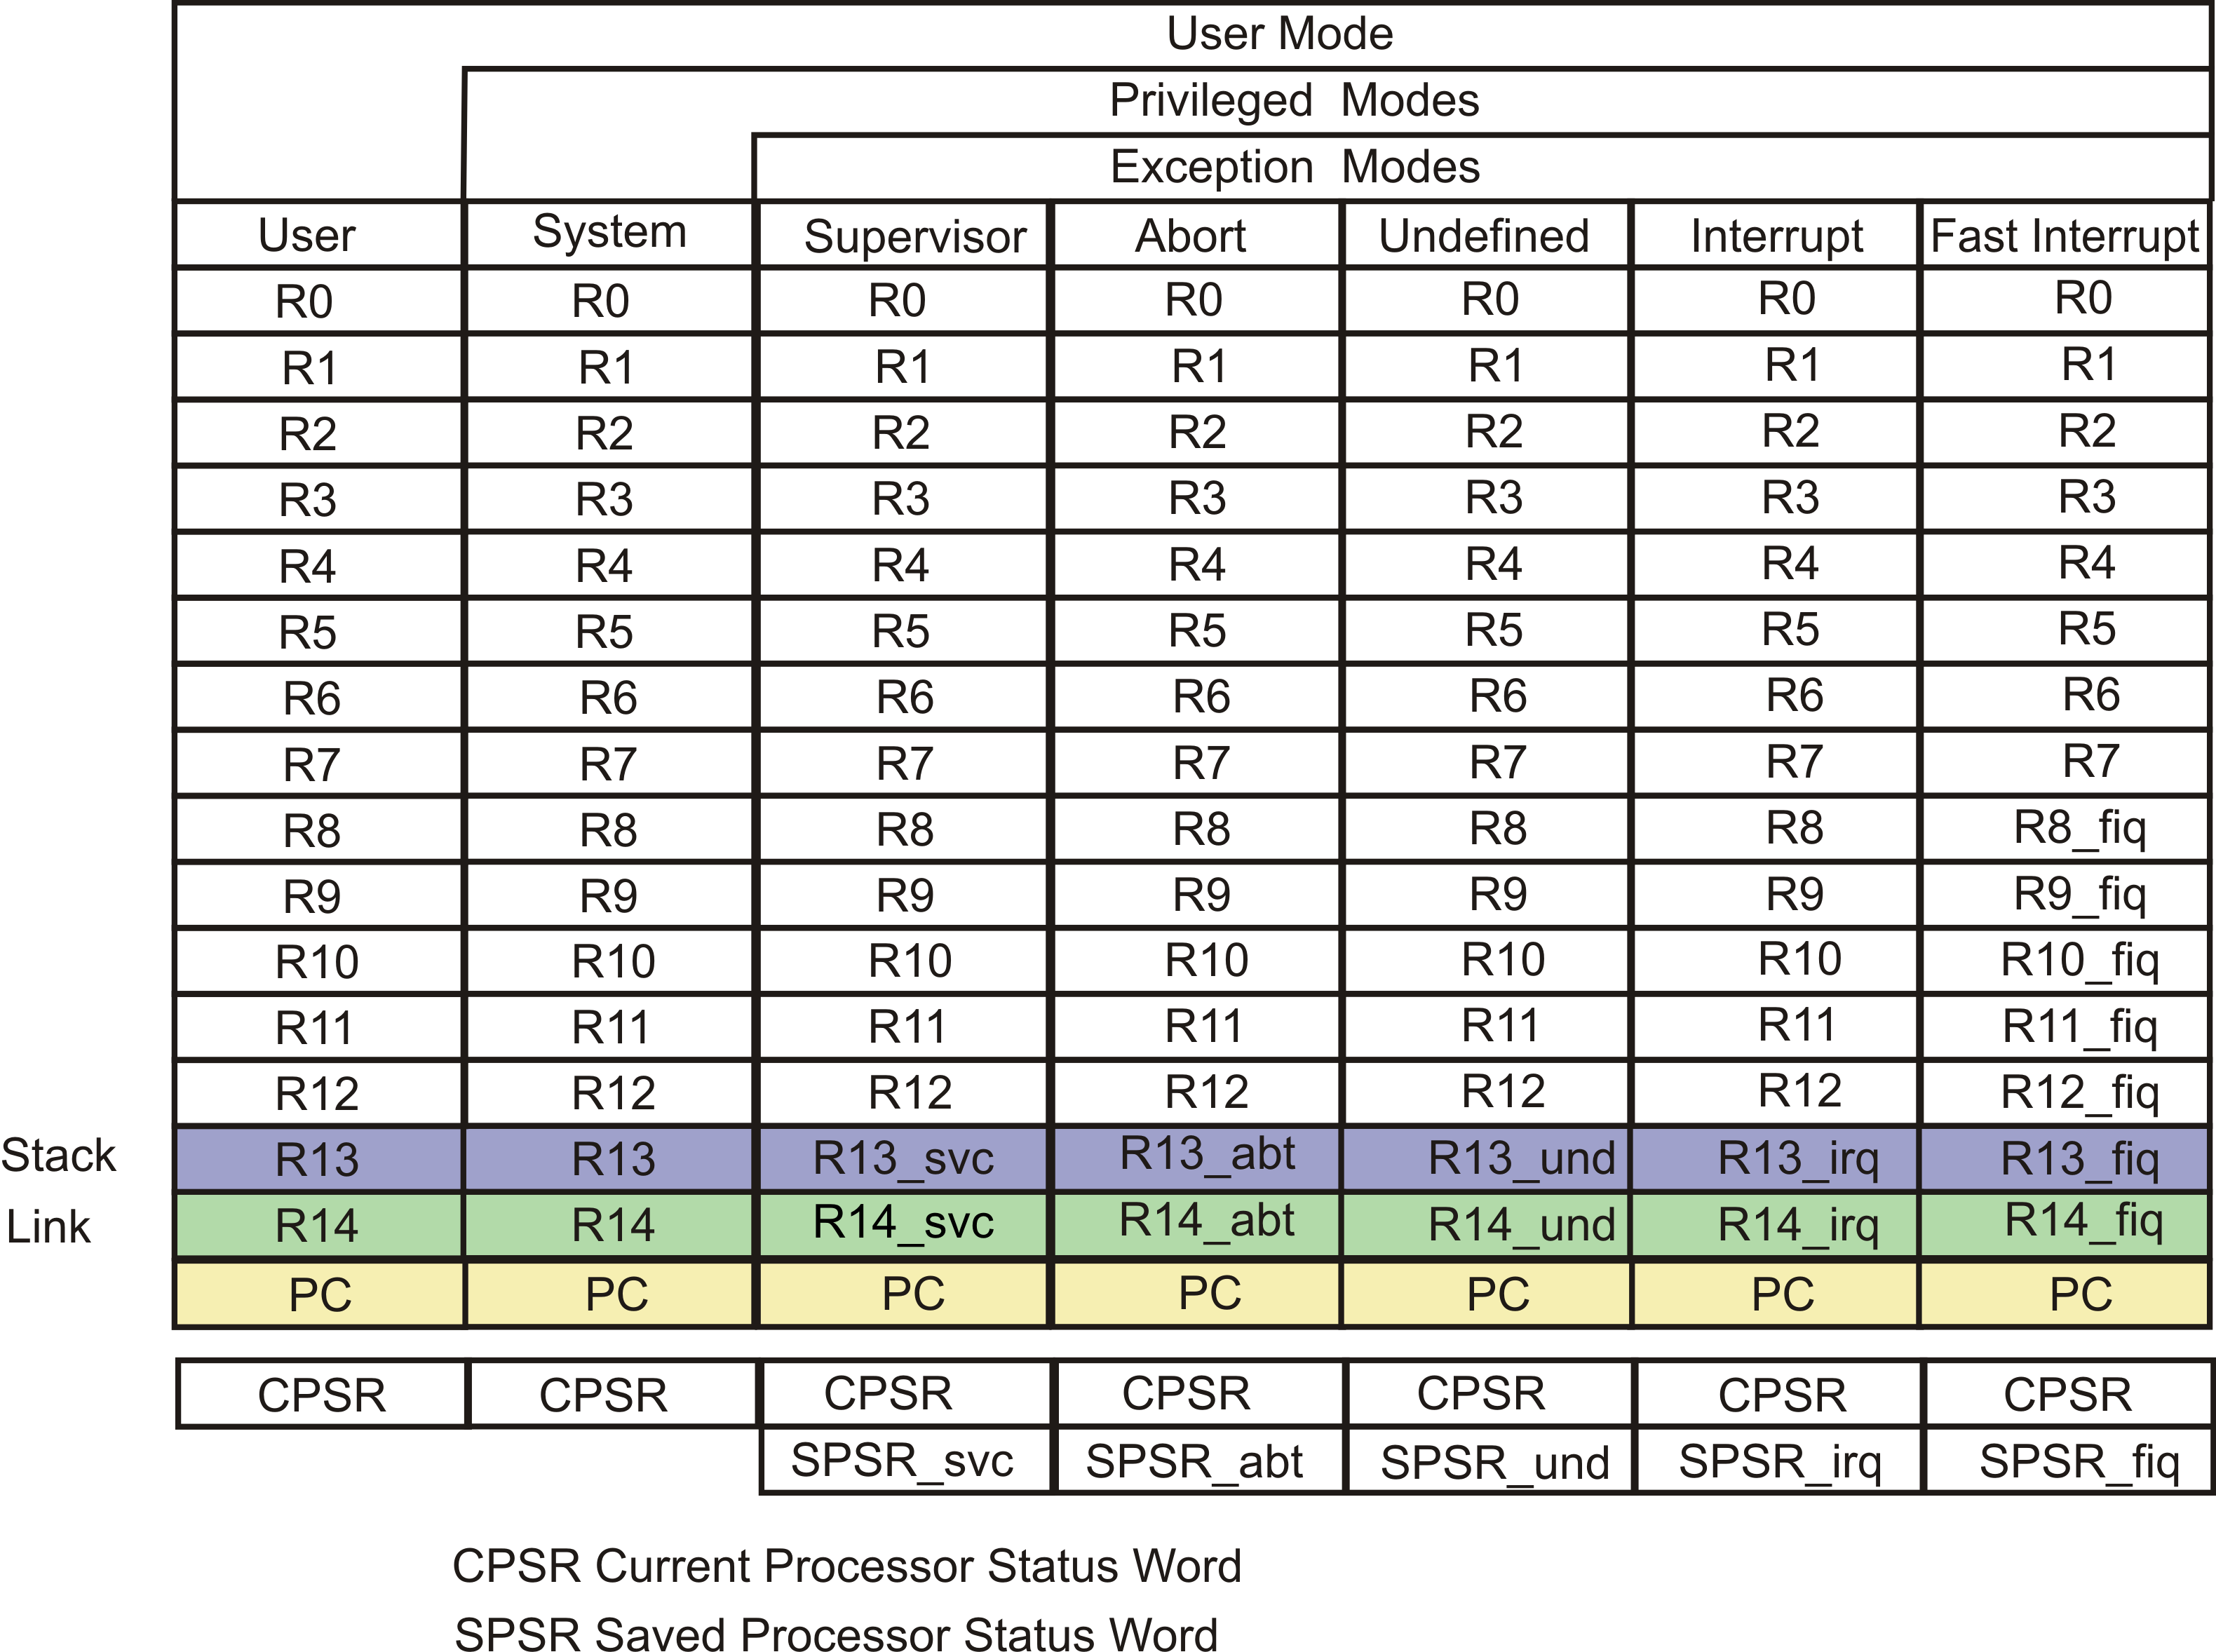
\epsfig{file=figures/Fig_3_10_RegisterSet.png,width=0.8\textwidth}\\
	  \caption{Register Set of the ALU}
     \end{center}
\end{figure}
\os{\newpage}

\bi
      \ite ALU (and the processor) runs in seven different modes
      \ite register set from r0 - r12 in every mode visible (without fast interrupt mode)
      \ite in exception modes the contains of the current processor status register (CPSR) are automatically saved (SPSR) (before the exception procedure starts) 
      \ite modes 
      \bi
		\ite user \pr standard mode
		\ite system \pr mode for operating systems
		\ite supervisor \pr mode for operating systems (mode after a reset)
		\ite abort \pr illegal instruction, illegal data operation
		\ite undefined \pr undefined instruction detected
		\ite interrupt \pr external interrupt
		\ite fast interrupt \pr internal interrupt (trap)
      \ei
\ei

\os{\newpage}
\item[{\rot\bf MAC (\underline{m}ultiply and \underline{ac}cumulate}]~\\[-3ex]

\bi 
	\ite part of the standard multiply function 
	\ite supports a multiplication and a add-operation in one instruction
	\ite different wordlength and signed/unsigned numbers are supported
	\ite typical examples (wordlength)
	\bi 
		\ite 32 = 32 +/- 16 x 16.
		\ite 32 = 32 + 16 x 16 + 16 x 16
		\ite 32 = 16 x 16
		\ite 64 = 64 +/- 32 x 32
		\ite 64 = 64 +/- 16 x 16
		\ite 64 = 32 x 32
	\ei
 
\ei
\os{\newpage}
\item[{\rot\bf NEON / VFP (SIMD and vector processing of integer and floating point numbers)}]~\\[-3ex]
\bi 
	\ite supports integer (fix point) and floating point packed calculations (NEON) of 32 bit numbers
	\ite vector floating point numbers with 32 bit or 64 bit are processed by the VFP-unit
	\ite every floating point number is:
	\bi
		\ite normalized
		\ite there exists no carry bit or a doubling of the word format after a multiplication (very useful in combined arithmetical expressions)
		\ite every floating point number could be characterized (zero, normalized, denormalized, exist, free) 
	\ei
	\bigskip
	\ite operations on NEON- and VFP-unit works as
	\bi
		\ite scalar operation on single (s = 32 bit), double (d = 64 bit) or quad q = 128 bit) precision, the involved registers have not be placed at the beginning of a bank
		\ite vector operations on 4 single precision elements, the involved registers starts at the beginning ore in the middle of a bank
		\ite vector operations on 2 double precision elements, in this case the registers starts at the beginning ore in the middle of a bank
		\ite scalar operation on 1 quad precision element
	\ei
\ei
\os{\newpage}
\begin{figure}[!hbtp]
     \begin{center}
	  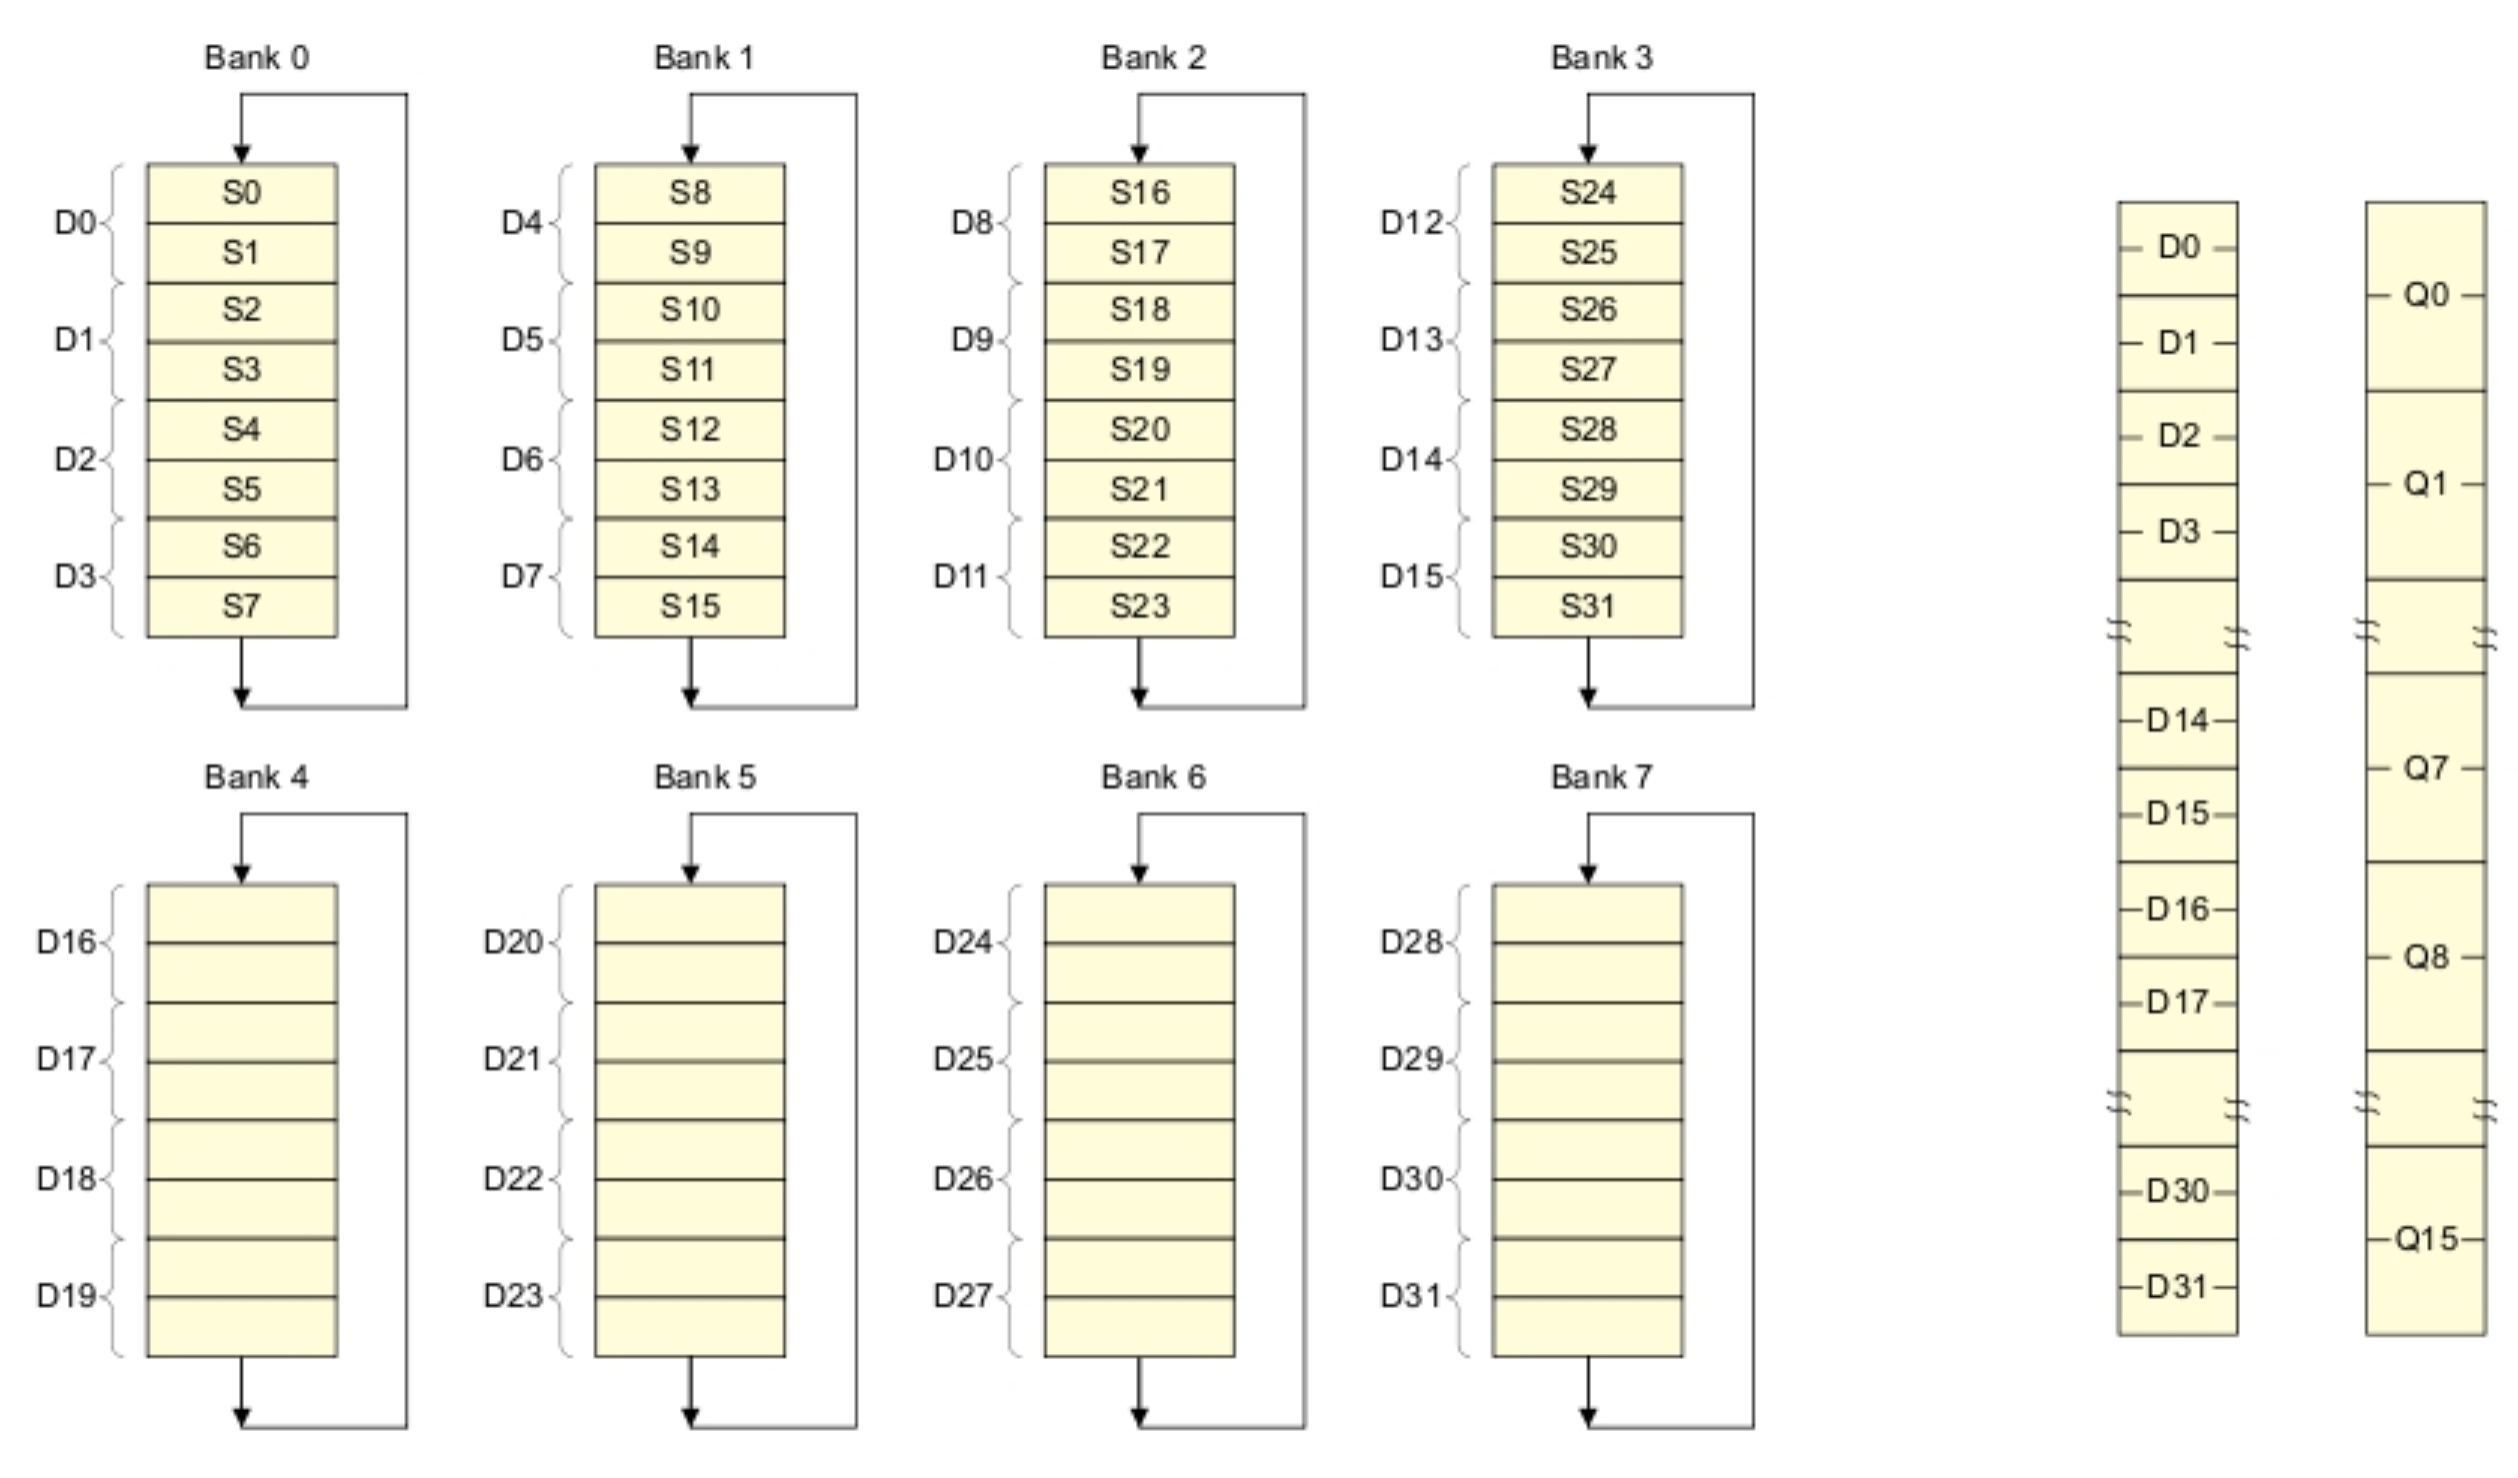
\epsfig{file=figures/Fig_3_11_NEON_VFP_Registers,width=0.9\textwidth}\\
	  \caption{Register set of NEON/VFP Coprocessor}
     \end{center}
\end{figure}
\os{\newpage}
 

\bi 
	\ite Examples for scalar and vector operations 
	\bi
		\ite scalar operation
		\ite FADDS S12, S21, S22
	\ei
	\bigskip
	\bi 
		\ite vector operation on single presision with 4 iterations
		\ite  FMACS S16, S0, S8 (instruction)
		\bigskip
		\\ FMACS S16, S0, S8  ; 1st iteration
		\\ FMACS S17, S1, S9  ; 2nd iteration
		\\ FMACS S18, S2, S10 ; 3rd iteration
		\\ FMACS S19, S3, S11 ; 4rd and last iteration
	\ei
	\bi 
		\ite vector operation on double presision with 2 iterations
		\ite  FMULD D12, D8, D2 (instruction)
		\bigskip
		\\ FMULD D12, D8, D2 ; 1st iteration
		\\ FMULD D13, D9, D3 ; 2nd and last iteration

	\ei 
\ei

\os{\newpage}
\item[{\rot\bf MMU (\underline{m}emory \underline{m}anagement \underline{u}nit) }]~\\[-3ex]

\bi 
	\ite supports a flexible, software-defined virtual environment.
	\ite in the case of virtual memory, the MMU supports 4-, 8-Kbyte, 1-Mbyte or 16-Mbyte page sizes.
	\ite the pages addressed with separate, 32-entry, fully associative instruction and data TLBs (TLBs \underline{t}ranslation \underline{l}ookaside \underline{b}uffer).
	\bi 
		\ite the separation of instruction- and data-TLB allows a parallel access of both instructions and data (Harvard-architecture).
		\ite the TLB works as registers (faster than memory based entries) 
	\ei
	\ite the MMU itself is memory-mapped (control, status, and fault registers)
	\ite the access to the MMU starts with a control-register 
	\ite MMU supports programmable address space priorisation steps (ASID \underline{a}ddress \underline{s}pace \underline{id}entifier).
\ei
\os{\newpage}
\begin{figure}[!hbtp]
     \begin{center}
	  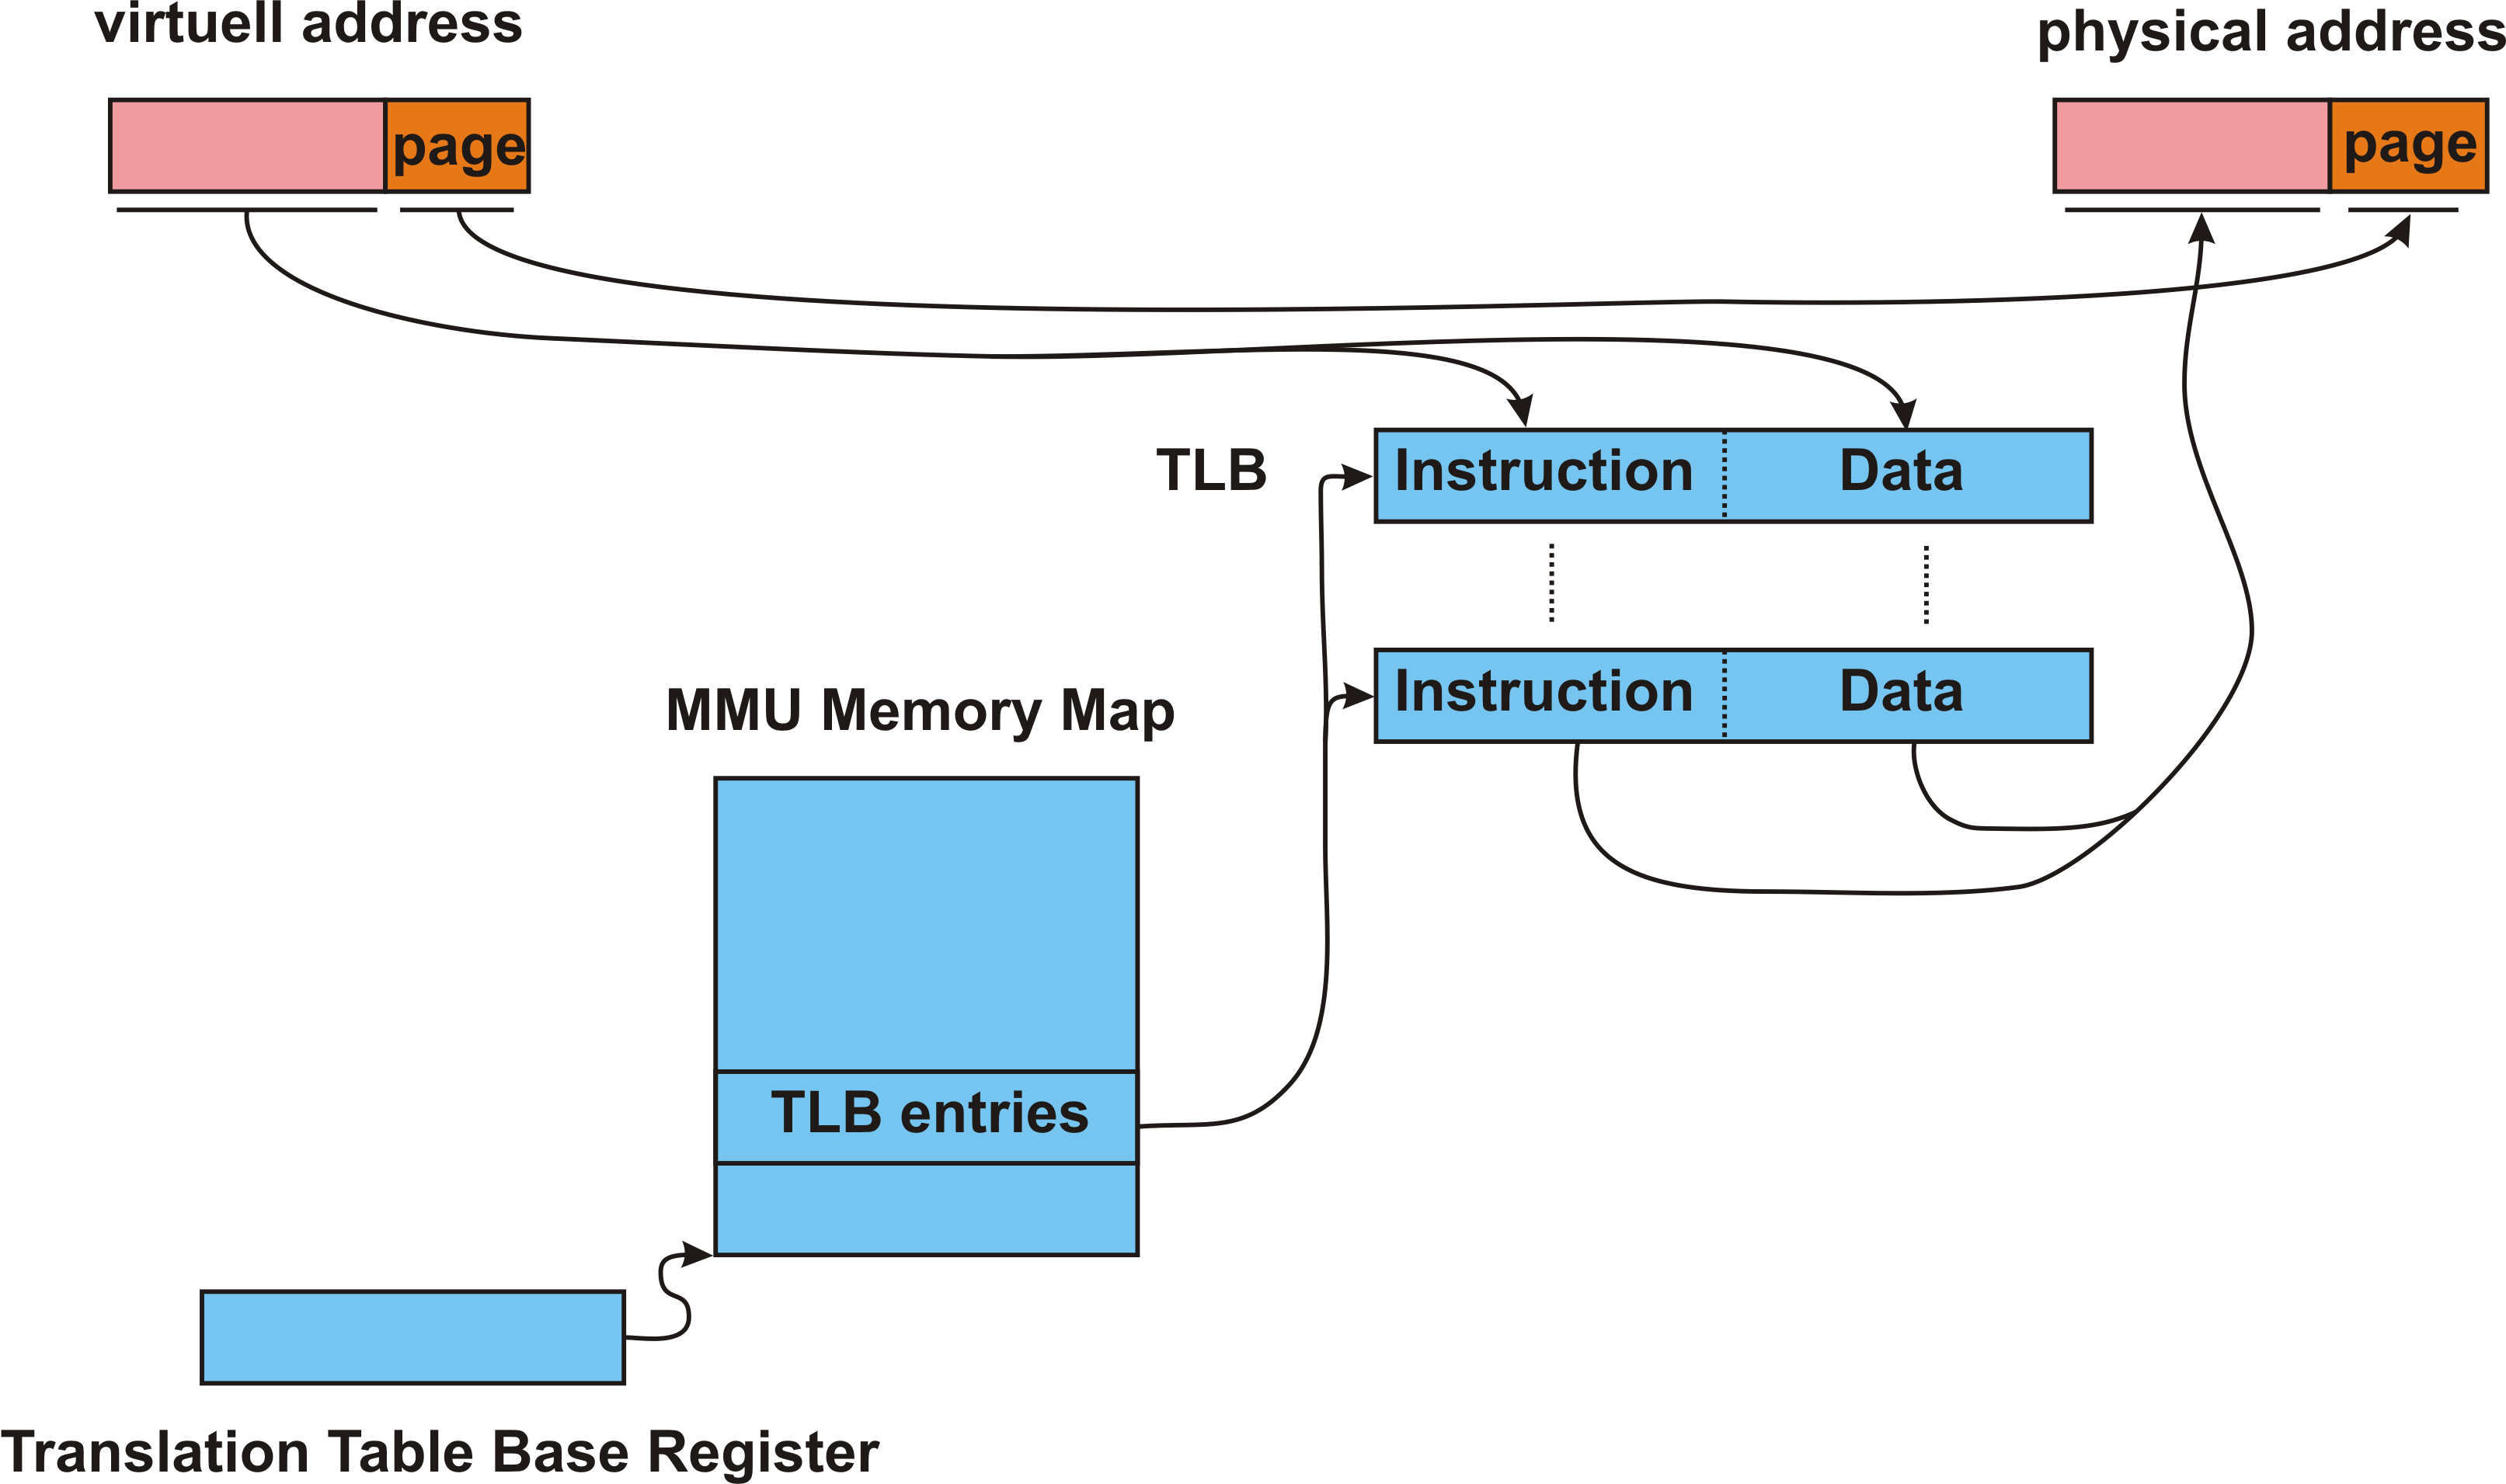
\epsfig{file=figures/Fig_3_12_MMU,width=0.8\textwidth}\\
	  \caption{Principal functions of the MMU}
     \end{center}
\end{figure}
\os{\newpage}

\begin{figure}[!hbtp]
     \begin{center}
	  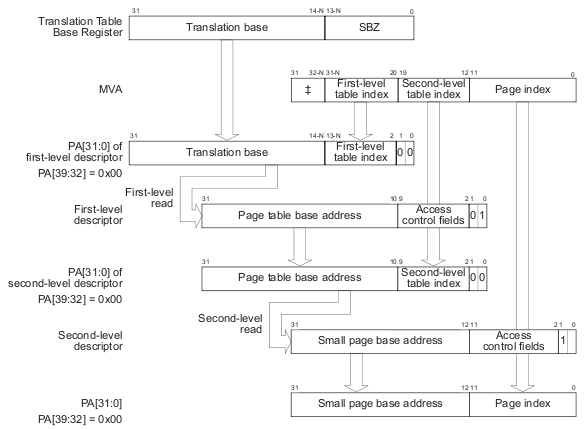
\epsfig{file=figures/Fig_3_13_Page_Address_Translation,width=0.8\textwidth}\\
	  \caption{Page Address Translation}
     \end{center}
\end{figure}
\os{\newpage}
\end{description}

%%%%%%%%%%%%%%%%%%%%%%%%%%%%%%%%%%%%%%%%%%%%%%%%%%%%%%%%%%%%%%%%%%%%%%%%%%%
\section{Overview about the DSP}
%%%%%%%%%%%%%%%%%%%%%%%%%%%%%%%%%%%%%%%%%%%%%%%%%%%%%%%%%%%%%%%%%%%%%%%%%%%
\begin{description}
\bigskip
\item[{\rot\bf DSP Functions and additional Features }]~\\[-3ex]
\bigskip
\bi
	\ite DSP supports the OMAP-Processors with   
	\bi 
		\ite processor funtionality to work on digital signal algorithm
		\ite internal RAM and ROM (data memory, Boot-ROM)
		\ite external RAM (SDRAM for instruction and data memory)
		\ite a lot of digital interfaces
	\ei
	\ite DSP is a 32 bit fix point processor
	 
\ei

\os{\newpage}
\begin{figure}[!hbtp]
     \begin{center}
	  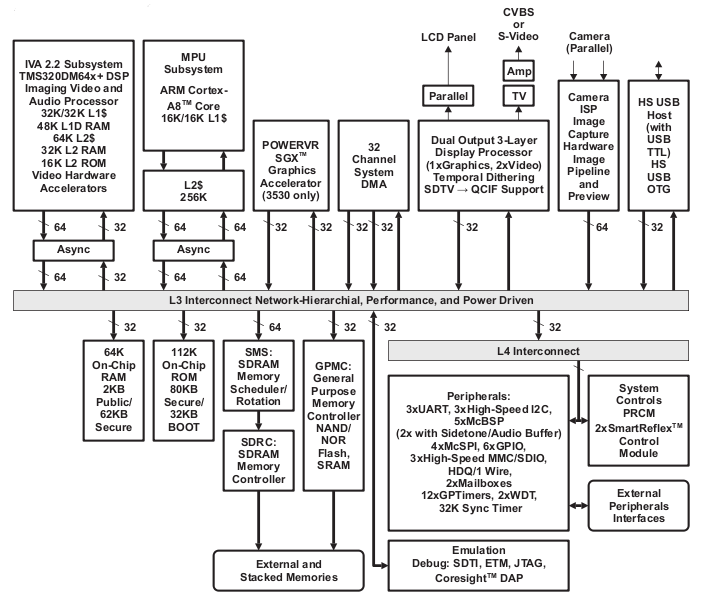
\epsfig{file=figures/Fig_3_14_OMAP_Blockdiagram,width=0.7\textwidth}\\
	  \caption{Overview about the Units in a OMAP-Processors}
     \end{center}
\end{figure}
\os{\newpage}

\item[{\rot\bf DSP (\underline{d}igital \underline{s}ignal \underline{p}rocessing) }]~\\[-3ex]
\bigskip
\bi
	\ite DSP processor with 64 x 32 bit registers grouped in two banks (bank A and bank B)
	\ite multiply add operational unit (MAC) (with a internal wordlength of 40 bits)
	\ite barrel shifter to scale the result
	\ite use internal memories (on the DSP-chip) to store up to 3 operands in 1 cycle
	\ite MAC-operation and barrel shifting-operation execute in 1 cycle
	\ite different interfaces for
	\bi 
		\ite connection to an external SDRAM
		\ite L2 cache system to coordinate parallel data transfers (for the transfer of both values in a multiplikation instruction)
		\ite internal timers
		\ite interrupt sources
	\ei
	\ite DSP is a VLIW-processor (\underline{v}ery \underline{l}ong \underline{i}nstruction \underline{w}ord)
	\bi
		\ite wordlength 256 bit
		\ite more instructions are placed in one instruction word (e.g. 2 transfers 4 arithmetical instructions)
		\ite one VLIW-instruction are excuted in one cycle
	\ei
\ei
\os{\newpage}
\begin{figure}[!hbtp]
     \begin{center}
	  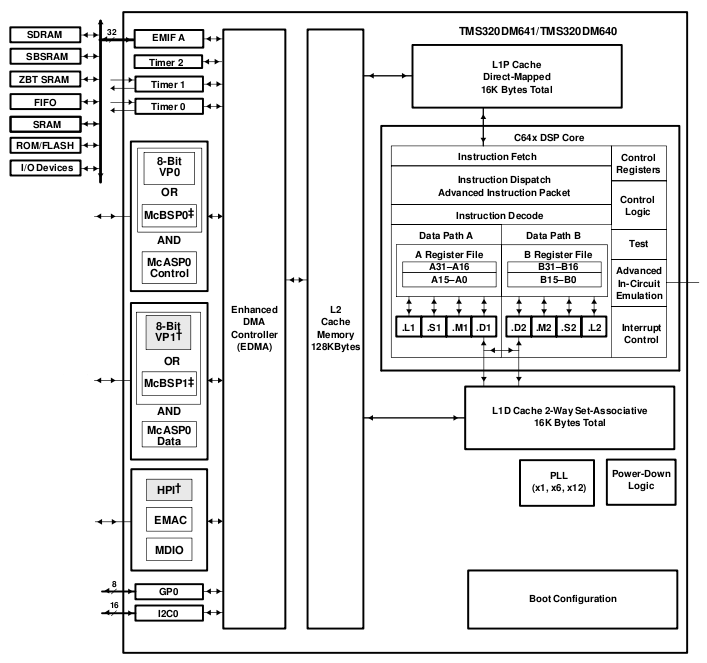
\epsfig{file=figures/Fig_3_15_Blockdiagram_TMS320DM641,width=0.6\textwidth}\\
	  \caption{Blockdiagram of the DSP-Part of the OMAP-Processor}
     \end{center}
\end{figure}
\os{\newpage}

\item[{\rot\bf I/O-Units }]~\\[-3ex]
\bigskip

\bi
      \ite additional to the processor (ARM-Cortex-A8) and the signal processor (DSP) many digital I/O-units implemented
      \ite all units are connected by two interprocessor busses (L3 and L4)
      \ite the communication are controlled by specific cache controllers and the according cache memories
      \ite all processors (internal memories) and the registers or memories of the I/O-units and the external memory are visible in the Global Memory Map
\ei 
\os{\newpage}
\begin{figure}[!hbtp]
     \begin{center}
	  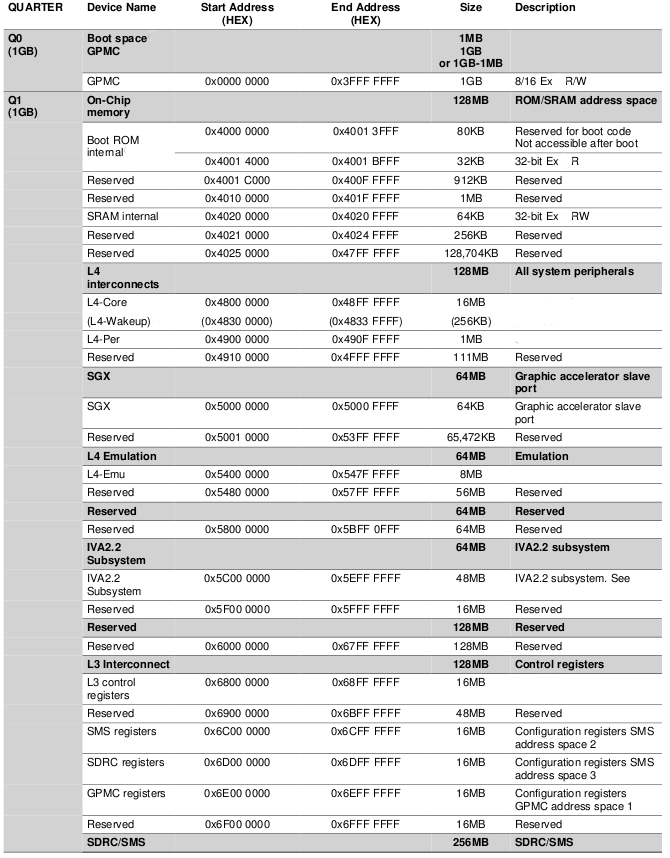
\epsfig{file=figures/Fig_3_16_MemoryMap_A,width=0.4\textwidth}\\
	  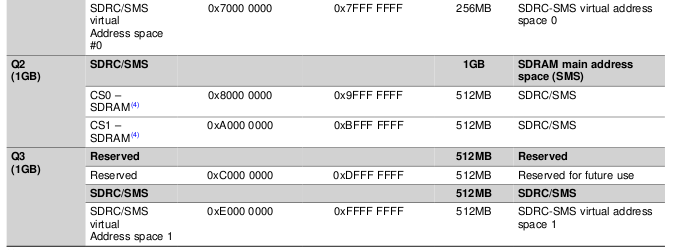
\epsfig{file =figures/Fig_3_16_MemoryMap_B,width=0.4\textwidth}\\
	  \caption{Global Memory Map of the OMAP-Processor}
     \end{center}
\end{figure}
\os{\newpage}

\bigskip
\bi
	\ite L3 interprocessor communication bus connects the processors and memory subsystems
	\ite L4 interprocessor communication bus connnects the processors with the I/O-systems
\ei
\os{\newpage}
\os{\bigskip}
\begin{figure}[!hbtp]
     \begin{center}
	  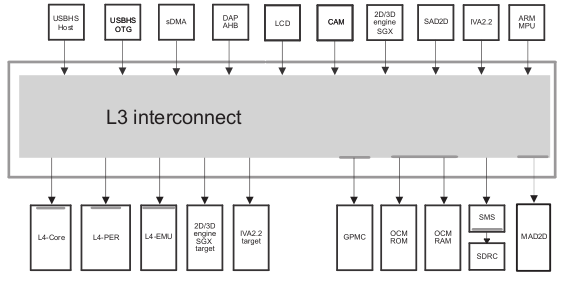
\epsfig{file=figures/Fig_3_17_L3_Interconnect,width=0.70\textwidth}\\
	  \caption{L3 Interprocessor Communication Bus}
     \end{center}
\end{figure}
\os{\newpage}

\begin{figure}[!hbtp]
     \begin{center}
	  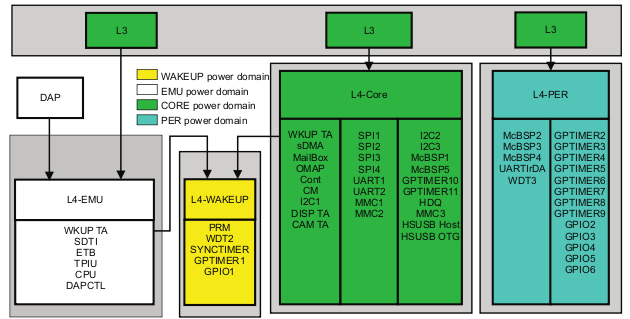
\epsfig{file=figures/Fig_3_18_L4_Interconnect,width=0.70\textwidth}\\
	  \caption{L4 Interprocessor Communication Bus}
     \end{center}
\end{figure}
\os{\newpage}

\bi
	\ite interprocessor communication and the communication between processors and the I/O-units are controlled by mailboxes
\ei

\os{\newpage}
\begin{figure}[!hbtp]
     \begin{center}
	  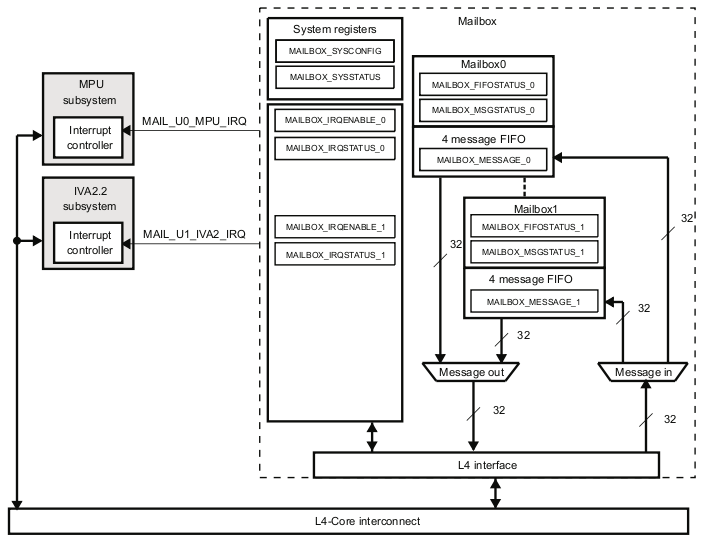
\epsfig{file=figures/Fig_3_19_Communication_Mailbox,width=0.70\textwidth}\\
	  \caption{Communication Mailbox}
     \end{center}
\end{figure}

\os{\newpage}
\begin{figure}[!hbtp]
     \begin{center}
	  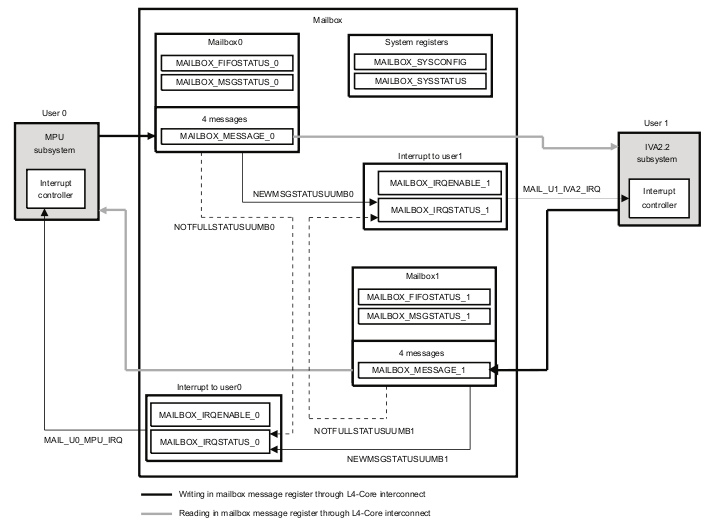
\epsfig{file=figures/Fig_3_20_Communication_Example,width=0.70\textwidth}\\
	  \caption{Example for Communications with Mailboxes}
     \end{center}
\end{figure}
\end{description}



%%%%%%%%%%%%%%%%%%%%%%%%%%%%%%%%%%%%%%%%%%%%%%%%%%%%%%%%%%%%%%%%%%%%%%%%%%
\chapter{Programming}
%%%%%%%%%%%%%%%%%%%%%%%%%%%%%%%%%%%%%%%%%%%%%%%%%%%%%%%%%%%%%%%%%%%%%%%%%%%
% Chapter: Programming
% Examples: examples/programming (assembly on the Pico in C and Rust, a
% host-tested Rust library, MicroPython, Python, C register access)
%%%%%%%%%%%%%%%%%%%%%%%%%%%%%%%%%%%%%%%%%%%%%%%%%%%%%%%%%%%%%%%%%%%%%%%%%%%

%%%%%%%%%%%%%%%%%%%%%%%%%%%%%%%%%%%%%%%%%%%%%%%%%%%%%%%%%%%%%%%%%%%%%%%%%%%
\section{From Source Code to Firmware}
%%%%%%%%%%%%%%%%%%%%%%%%%%%%%%%%%%%%%%%%%%%%%%%%%%%%%%%%%%%%%%%%%%%%%%%%%%%
\nsl{Embedded software is developed on a PC and runs on a different
processor: it is cross-compiled. The toolchain translates the source code
into machine code for the target, the linker places code and data at the
addresses of the target's memory, and a programming tool writes the result
into the flash. This chapter starts with these steps. Then it looks at the
languages used in this lecture, from assembly through C and Rust to
MicroPython, and ends with systematic debugging. Several examples run on the
Raspberry Pi Pico in Wokwi again.
\newpage}

\begin{description}
\item[{\rot\bf The build process}]~\\[-3ex]
\begin{figure}[!hbtp]
\begin{center}
\resizebox{0.95\textwidth}{!}{%
\begin{tikzpicture}[font=\sffamily\small,>=Stealth,
	b/.style={draw,thick,rounded corners,minimum height=10mm,text width=20mm,align=center}]
	\node[b,fill=gray!10] (src) at (0,0) {source\\.c .rs .S};
	\node[b,fill=blue!10] (cc) at (3,0) {compiler /\\assembler};
	\node[b,fill=gray!10] (obj) at (6,0) {object files\\.o};
	\node[b,fill=blue!10] (ld) at (9,0) {linker};
	\node[b,fill=gray!10] (elf) at (12,0) {ELF file};
	\node[b,fill=green!10] (img) at (15,0) {.bin / .hex\\/ .uf2};
	\node[b,fill=orange!15] (lds) at (9,-2) {linker script\\memory map};
	\node[b,fill=orange!15] (lib) at (6,-2) {libraries,\\start-up code};
	\draw[->,thick] (src) -- (cc); \draw[->,thick] (cc) -- (obj); \draw[->,thick] (obj) -- (ld);
	\draw[->,thick] (ld) -- (elf); \draw[->,thick] (elf) -- node[above,font=\sffamily\scriptsize]{objcopy} (img);
	\draw[->,thick] (lds) -- (ld); \draw[->,thick] (lib) -- (ld);
\end{tikzpicture}}
\caption{From source code to the image in the flash}
\end{center}
\end{figure}
\bi
	\ite \textbf{cross compiler}, named after the target: \texttt{arm-none-eabi-gcc} (ARM, no OS), \texttt{riscv32-esp-elf-gcc}; in Rust a target triple such as \texttt{thumbv6m-none-eabi}
	\ite the \textbf{linker} combines all object files and assigns addresses according to the linker script (\texttt{memory.x} in our Rust examples: flash at 0x1000\,0000, RAM at 0x2000\,0000)
	\ite the \textbf{ELF} file contains code, data, symbols and debug information -- the debugger needs it; the flash only needs the raw image
\ei
\os{\newpage}

\item[{\rot\bf Sections and start-up}]~\\[-3ex]
\bi
	\ite \texttt{.text}: machine code (flash); \texttt{.rodata}: constants (flash)
	\ite \texttt{.data}: initialised variables -- the initial values are in flash, the variables in RAM
	\ite \texttt{.bss}: variables initialised with zero (RAM only)
	\ite the \textbf{start-up code} runs before \texttt{main}: set the stack pointer (from the vector table), copy \texttt{.data} from flash to RAM, fill \texttt{.bss} with zeros, set up clocks, then call \texttt{main}
	\ite in Rust \texttt{cortex-m-rt} provides this code and the attribute \texttt{\#[entry]}
\ei
\begin{lstlisting}[language={}]
$ llvm-size -A target/thumbv6m-none-eabi/release/gpio_blink   # addresses in hex
section        size        addr
.vector_table   192   0x10000100
.boot2          256   0x10000000      <- 2nd stage bootloader of the RP2040
.text          2940   0x100001c0
.rodata         360   0x10000b3c
.bss              4   0x20000000
\end{lstlisting}
\bi
	\ite the same blink program with the Arduino core: about 314\,KB code -- the core always links USB, serial and file system support
\ei
\os{\newpage}

\item[{\rot\bf Getting the program onto the chip}]~\\[-3ex]
\bi
	\ite \textbf{bootloader in ROM} or flash: receives the image over USB or UART
	\bi
		\ite RP2040: hold BOOTSEL, the Pico appears as a USB drive -- copy a \texttt{.uf2} file onto it
		\ite ESP32: ROM bootloader via the serial port (\texttt{esptool}, \texttt{espflash})
	\ei
	\ite \textbf{debug probe} via SWD or JTAG (see section Debugging): programming and debugging with the same cable
	\ite in production: programming on the panel, in-circuit test, unique keys and serial numbers per device
	\ite \textbf{over the air} updates: the running firmware downloads a new image into a second flash partition and switches after a check -- needs a bootloader that can roll back
\ei
\os{\newpage}
\end{description}

%%%%%%%%%%%%%%%%%%%%%%%%%%%%%%%%%%%%%%%%%%%%%%%%%%%%%%%%%%%%%%%%%%%%%%%%%%%
\section{Programming in Assembly}
%%%%%%%%%%%%%%%%%%%%%%%%%%%%%%%%%%%%%%%%%%%%%%%%%%%%%%%%%%%%%%%%%%%%%%%%%%%
\nsl{Today almost nobody writes complete programs in assembly. Compilers
generate good code, and C and Rust are portable and much easier to maintain.
Still, every embedded developer must be able to read assembly. You need it
to understand what the compiler made of your code, to analyse a crash in
the debugger, and to write the few parts that cannot be expressed in a high
level language, such as start-up code, context switches and special
instructions. We use the Cortex-M0+ of the RP2040 as our example. Its
instruction set (Thumb, ARMv6-M) is small enough to be learned in a few
hours.}

\begin{description}
\item[{\rot\bf Registers of the Cortex-M0+}]~\\[-3ex]
\bi
	\ite 16 registers of 32 bit
	\bi
		\ite \texttt{r0}--\texttt{r12}: general purpose (most 16 bit instructions can only use \texttt{r0}--\texttt{r7})
		\ite \texttt{r13} = \texttt{sp}: stack pointer (two of them: main and process stack)
		\ite \texttt{r14} = \texttt{lr}: link register, return address of a function call
		\ite \texttt{r15} = \texttt{pc}: program counter
	\ei
	\ite \textbf{xPSR} status register with the flags of the last arithmetic instruction
	\bi
		\ite \textbf{N} negative, \textbf{Z} zero, \textbf{C} carry (unsigned overflow), \textbf{V} overflow (signed)
		\ite only instructions with an \texttt{s} suffix (\texttt{adds}, \texttt{subs}) and comparisons (\texttt{cmp}) set the flags
	\ei
	\ite all data processing works on registers -- memory only via \texttt{ldr}/\texttt{str} (load/store architecture)
\ei
\os{\newpage}

\item[{\rot\bf Instructions (selection)}]~\\[-3ex]
\begin{center}
\resizebox{\textwidth}{!}{%
\begin{tabular}{|l|l|l|}
\hline
\textbf{group} & \textbf{examples} & \textbf{meaning} \\
\hline
move & \texttt{movs r0, \#5} \quad \texttt{mov r1, r2} & r0 = 5 (8 bit immediate), r1 = r2 \\
arithmetic & \texttt{adds r0, r1, r2} \quad \texttt{subs r1, r1, \#1} \quad \texttt{muls r0, r1} & r0 = r1 + r2, r1 = r1 - 1, r0 = r0 $\cdot$ r1 \\
logic, shift & \texttt{ands r0, r1} \quad \texttt{orrs} \quad \texttt{eors} \quad \texttt{lsls r0, r0, \#2} & bitwise AND, OR, XOR; shift left \\
compare & \texttt{cmp r1, \#0} \quad \texttt{cmp r3, r1} & compute r1 - 0, set flags only \\
load & \texttt{ldr r0, [r1]} \quad \texttt{ldrh r3, [r0, \#2]} \quad \texttt{ldrb r2, [r0, r1]} & 32 / 16 / 8 bit from memory \\
store & \texttt{str r0, [r1, \#4]} \quad \texttt{strh} \quad \texttt{strb} & 32 / 16 / 8 bit to memory \\
constant & \texttt{ldr r0, =0xd000001c} & 32 bit constant from a literal pool in flash \\
stack & \texttt{push \{r4, lr\}} \quad \texttt{pop \{r4, pc\}} & save registers / restore and return \\
branch & \texttt{b label} \quad \texttt{beq} \quad \texttt{bne} \quad \texttt{blt} \quad \texttt{bhs} & jump, conditional on the flags \\
call, return & \texttt{bl function} \quad \texttt{bx lr} & call (return address in lr), return \\
\hline
\end{tabular}}
\end{center}
\bi
	\ite conditions: \texttt{eq}/\texttt{ne} (Z), signed \texttt{lt}/\texttt{ge}/\texttt{gt}/\texttt{le}, unsigned \texttt{lo}/\texttt{hs}/\texttt{hi}/\texttt{ls}
\ei
\os{\newpage}

\item[{\rot\bf Calling convention (AAPCS)}]~\\[-3ex]
\bi
	\ite the rules that let C, Rust and assembly functions call each other
	\ite arguments in \texttt{r0}--\texttt{r3}, further arguments on the stack
	\ite return value in \texttt{r0} (64 bit values in \texttt{r0}+\texttt{r1})
	\ite \texttt{r0}--\texttt{r3} and \texttt{r12} may be changed by the called function (caller-saved)
	\ite \texttt{r4}--\texttt{r11} must have the same value after the call (callee-saved) -- save them with \texttt{push} if you use them
	\ite the stack grows downwards and is 8 byte aligned at function calls
	\ite the RISC-V equivalent: arguments in \texttt{a0}--\texttt{a7}, return value in \texttt{a0}, callee-saved \texttt{s0}--\texttt{s11}, return address in \texttt{ra}
\ei
\os{\newpage}

\item[{\rot\bf Our own assembly function}]~\\[-3ex]
\begin{lstlisting}[language={}]
@ uint32_t asm_sum(const uint16_t *a, int n)    file sum_m0.S
@ AAPCS: a in r0, n in r1, result in r0. Only r0..r3 are used.
    .syntax unified
    .cpu cortex-m0plus
    .thumb
    .global asm_sum
    .type   asm_sum, %function
    .thumb_func
asm_sum:
    movs  r2, #0          @ s = 0
    cmp   r1, #0
    ble   2f              @ n <= 0: nothing to do
1:  ldrh  r3, [r0]        @ r3 = *a
    adds  r0, r0, #2      @ a++ (2 bytes)
    adds  r2, r2, r3      @ s += r3
    subs  r1, r1, #1      @ n--, sets the Z flag
    bne   1b              @ loop while n != 0
2:  movs  r0, r2          @ return s
    bx    lr
\end{lstlisting}
\bi
	\ite 5 instructions in the loop instead of 7 from the compiler (chapter Processors): counting down saves the compare
\ei
\os{\newpage}

\item[{\rot\bf Calling it from C and from Rust}]~\\[-3ex]
\begin{lstlisting}[language=C]
extern "C" uint32_t asm_sum(const uint16_t *a, int n);   // C linkage

const uint16_t data[] = {1, 2, 3, 1000, 60000, 65535};
Serial1.printf("asm_sum = %lu\n", (unsigned long)asm_sum(data, 6));

uint32_t sp;
asm volatile("mov %0, sp" : "=r"(sp));   // inline assembly (GCC syntax)
\end{lstlisting}
\begin{lstlisting}[language=Rust]
global_asm!(".global asm_sum", /* ... the same instructions ... */);
unsafe extern "C" {
    fn asm_sum(a: *const u16, n: i32) -> u32;
}
let s_asm = unsafe { asm_sum(data.as_ptr(), data.len() as i32) };

let mut x: u32 = 40;
unsafe { asm!("adds {0}, {0}, {1}", inout(reg) x, in(reg) 2u32) };
\end{lstlisting}
\bi
	\ite output in Wokwi (both languages): \texttt{asm\_sum = 126541}, identical to the C and Rust versions
	\ite Rust marks every call into assembly as \texttt{unsafe}: the compiler cannot check it
\ei
\os{\newpage}
\end{description}

%%%%%%%%%%%%%%%%%%%%%%%%%%%%%%%%%%%%%%%%%%%%%%%%%%%%%%%%%%%%%%%%%%%%%%%%%%%
\section{C for Embedded Systems}
%%%%%%%%%%%%%%%%%%%%%%%%%%%%%%%%%%%%%%%%%%%%%%%%%%%%%%%%%%%%%%%%%%%%%%%%%%%
\nsl{C is still the most widely used language for microcontrollers. It is
close to the hardware, every chip vendor supports it, and almost all
existing code is written in it. On the other hand C checks very little. Out
of bounds accesses, integer overflows and use of freed memory compile
without complaint and lead to errors that are hard to find. Embedded C is
therefore usually written following coding rules, compiled with all
warnings enabled and checked with static analysis tools.}

\begin{description}
\item[{\rot\bf Data types and qualifiers}]~\\[-3ex]
\bi
	\ite \texttt{int} has 16 bit on the AVR and 32 bit on ARM $\Rightarrow$ use the fixed width types of \texttt{<stdint.h>}: \texttt{uint8\_t}, \texttt{int16\_t}, \texttt{uint32\_t}, \ldots
	\ite \texttt{volatile}: every access really happens -- for hardware registers and variables shared with interrupts
	\ite \texttt{const}: read only; on most MCUs \texttt{const} data stays in flash and saves RAM
	\ite \texttt{static} at file level: visible only in this file -- the C way of encapsulation
	\ite integer pitfalls
	\bi
		\ite signed overflow is undefined behaviour: the compiler may assume it never happens
		\ite shifting by the width of the type or more is undefined: \texttt{1 << 32}
		\ite integer promotion: \texttt{uint8\_t a = 200, b = 100; if (a + b > 255)} is true, because the sum is calculated as \texttt{int}
	\ei
\ei
\os{\newpage}

\item[{\rot\bf Registers as structures}]~\\[-3ex]
\begin{lstlisting}[language=C]
typedef struct {
    volatile uint32_t cpuid;          /* 0x000 */
    volatile uint32_t gpio_in;        /* 0x004 */
    volatile uint32_t gpio_hi_in;     /* 0x008 */
    uint32_t _reserved;               /* 0x00c */
    volatile uint32_t gpio_out;       /* 0x010 */
    volatile uint32_t gpio_out_set;   /* 0x014 */
    volatile uint32_t gpio_out_clr;   /* 0x018 */
    volatile uint32_t gpio_out_xor;   /* 0x01c */
    volatile uint32_t gpio_oe;        /* 0x020 */
    volatile uint32_t gpio_oe_set;    /* 0x024 */
} sio_hw_t;

#define sio_hw ((sio_hw_t *)0xd0000000u)

/* The compiler checks the offsets for us */
_Static_assert(__builtin_offsetof(sio_hw_t, gpio_out_xor) == 0x01c, "offset");

void led_toggle(unsigned pin) { sio_hw->gpio_out_xor = 1u << pin; }
\end{lstlisting}
\bi
	\ite the style of the Pico SDK and of the CMSIS headers of all ARM vendors; generated from the chip description (SVD file)
\ei
\os{\newpage}

\item[{\rot\bf Bit manipulation}]~\\[-3ex]
\begin{lstlisting}[language=C]
reg |=  (1u << 5);            // set bit 5
reg &= ~(1u << 5);            // clear bit 5
reg ^=  (1u << 5);            // toggle bit 5
if (reg & (1u << 5)) { }      // test bit 5

/* write a field of several bits (read - modify - write) */
static inline uint32_t set_field(uint32_t reg, unsigned shift, uint32_t mask, uint32_t value) {
    return (reg & ~(mask << shift)) | ((value & mask) << shift);
}
ctrl = set_field(ctrl, 4, 0x3u, 2u);   /* bits 5..4 := 2 */
\end{lstlisting}
\bi
	\ite always use unsigned constants (\texttt{1u}) -- \texttt{1 << 31} overflows a signed \texttt{int}
	\ite read-modify-write is not atomic: protect it against interrupts, or use SET/CLR registers if the hardware offers them
	\ite C bit fields (\texttt{uint32\_t mode : 2;}) are not portable for registers: the order of the bits is implementation-defined
\ei
\os{\newpage}

\item[{\rot\bf Rules for reliable C}]~\\[-3ex]
\bi
	\ite compile with all warnings and treat them as errors: \texttt{-Wall -Wextra -Werror}
	\ite no dynamic memory after start-up (\texttt{malloc}/\texttt{free}): fragmentation and failing allocations at run time
	\ite no recursion: the stack usage must be known
	\ite check every return value and every array index
	\ite coding standards: \textbf{MISRA C} (automotive and industry), CERT C (security) -- they forbid the dangerous constructs of the language
	\ite static analysis (e.g.\ \texttt{cppcheck}, \texttt{clang-tidy}, commercial tools), sanitizers and unit tests on the PC
	\ite these rules catch many errors -- Rust makes most of them impossible by construction (next section)
\ei
\os{\newpage}
\end{description}

%%%%%%%%%%%%%%%%%%%%%%%%%%%%%%%%%%%%%%%%%%%%%%%%%%%%%%%%%%%%%%%%%%%%%%%%%%%
\section{Rust for Embedded Systems}
%%%%%%%%%%%%%%%%%%%%%%%%%%%%%%%%%%%%%%%%%%%%%%%%%%%%%%%%%%%%%%%%%%%%%%%%%%%
\nsl{Rust is a systems programming language with the performance of C and
without a garbage collector, but with memory safety checked by the
compiler. A Rust program without \texttt{unsafe} blocks has no dangling
pointers, no out of bounds accesses and no data races. For embedded systems
it adds more: the type system can express hardware states, as we saw with
the GPIO pins in chapter 6. Cargo makes libraries and builds easy, and a
large ecosystem of hardware abstraction crates exists. Rust is now used in
the Linux kernel, and a qualified compiler (Ferrocene) is available for
safety-critical products. This section summarises the concepts we used in
the previous chapters and shows how to test embedded code on the PC.}

\begin{description}
\item[{\rot\bf Ownership and borrowing in five rules}]~\\[-3ex]
\bi
	\ite every value has exactly one \textbf{owner}; when the owner goes out of scope, the value is dropped (memory, peripherals, locks are released)
	\ite assignment or passing to a function \textbf{moves} the value: the old variable can no longer be used
	\ite instead of moving, a value can be \textbf{borrowed}: \texttt{\&T} (read, many at a time) or \texttt{\&mut T} (write, only one at a time)
	\ite a reference can never live longer than the value it points to
	\ite consequence: no use after free, no double free, and no two parts of a program changing the same data at the same time
\ei
\begin{lstlisting}[language=Rust]
let led = pins.gpio15.into_push_pull_output();
spawner.spawn(blink(led).unwrap());   // led is moved into the task
led.set_high();                       // error[E0382]: borrow of moved value: `led`
\end{lstlisting}
\os{\newpage}

\item[{\rot\bf Embedded Rust: no\_std and the layers}]~\\[-3ex]
\bi
	\ite \texttt{\#![no\_std]}: only the \texttt{core} library (no heap, no files, no threads); \texttt{alloc} can be added with an allocator
	\ite \texttt{\#![no\_main]} and \texttt{\#[entry]}: the start-up code calls our function; it never returns (\texttt{-> !})
	\ite a \textbf{panic handler} decides what happens on a panic: halt, print a backtrace, reset
\ei
\begin{figure}[!hbtp]
\begin{center}
\resizebox{0.8\textwidth}{!}{%
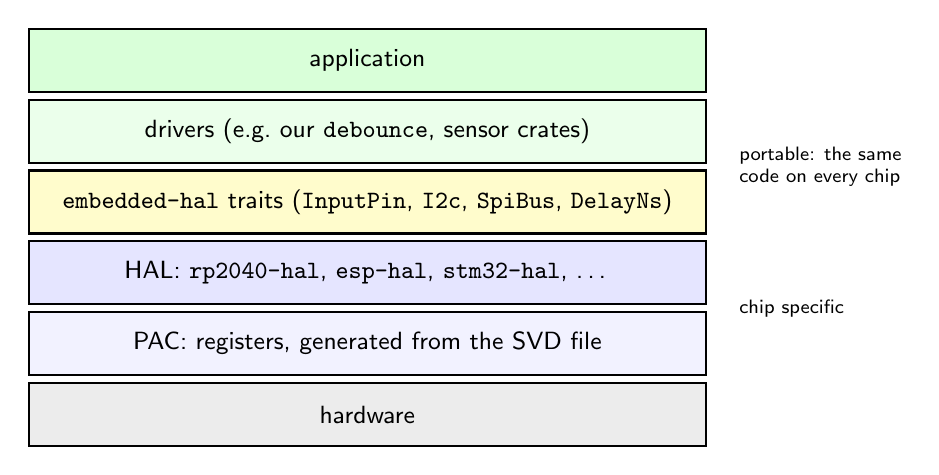
\begin{tikzpicture}[font=\sffamily\small,
	l/.style={draw,thick,minimum width=86mm,minimum height=8mm,align=center}]
	\node[l,fill=green!15] at (0,3.6) {application};
	\node[l,fill=green!8] at (0,2.7) {drivers (e.g.\ our \texttt{debounce}, sensor crates)};
	\node[l,fill=yellow!20] at (0,1.8) {\texttt{embedded-hal} traits (\texttt{InputPin}, \texttt{I2c}, \texttt{SpiBus}, \texttt{DelayNs})};
	\node[l,fill=blue!10] at (0,0.9) {HAL: \texttt{rp2040-hal}, \texttt{esp-hal}, \texttt{stm32-hal}, \ldots};
	\node[l,fill=blue!5] at (0,0) {PAC: registers, generated from the SVD file};
	\node[l,fill=gray!15] at (0,-0.9) {hardware};
	\node[right,font=\sffamily\scriptsize,align=left] at (4.6,2.25) {portable: the same\\code on every chip};
	\node[right,font=\sffamily\scriptsize,align=left] at (4.6,0.45) {chip specific};
\end{tikzpicture}}
\caption{Layers of the embedded Rust ecosystem}
\end{center}
\end{figure}
\os{\newpage}

\item[{\rot\bf A hardware independent driver}]~\\[-3ex]
\begin{lstlisting}[language=Rust]
#![no_std]
use embedded_hal::digital::InputPin;
pub enum Edge { None, Pressed, Released }
pub struct Debouncer { stable: bool, counter: u8, threshold: u8 }  // threshold = samples

impl Debouncer {
    pub fn update(&mut self, raw: bool) -> Edge {
        if raw == self.stable {
            self.counter = 0;
            return Edge::None;
        }
        self.counter += 1;
        if self.counter < self.threshold {
            return Edge::None;
        }
        self.counter = 0;
        self.stable = raw;
        if raw { Edge::Pressed } else { Edge::Released }
    }

    pub fn poll<P: InputPin>(&mut self, pin: &mut P) -> Result<Edge, P::Error> {
        Ok(self.update(pin.is_low()?))   // any pin type that implements InputPin
    }
}
\end{lstlisting}
\os{\newpage}

\item[{\rot\bf Testing embedded code on the PC}]~\\[-3ex]
\begin{lstlisting}[language=Rust]
#[test]
fn bouncing_gives_one_edge() {
    let mut d = Debouncer::new(3);
    // contact bounce: short pulses before the level is stable
    let samples = [true, false, true, false, true, true, true, true, true];
    assert_eq!(run(&mut d, &samples), (1, 0));
}

/// A fake pin for tests: implements the same trait as a real GPIO pin.
struct FakePin(bool);
impl InputPin for FakePin { /* is_high / is_low return self.0 */ }
\end{lstlisting}
\begin{lstlisting}[language={}]
$ cargo test
test tests::bouncing_gives_one_edge ... ok
test tests::clean_press_and_release ... ok
test tests::poll_reads_active_low_pin ... ok
test tests::short_glitch_is_ignored ... ok
test result: ok. 4 passed; 0 failed
\end{lstlisting}
\bi
	\ite the same library runs unchanged on the Pico (\texttt{button\_lib.rs}) -- logic is tested quickly on the PC (or Replit), only the hardware access needs the target
\ei
\os{\newpage}

\item[{\rot\bf Rust tools and practices}]~\\[-3ex]
\bi
	\ite \texttt{rustup target add thumbv6m-none-eabi} / \texttt{riscv32imc-unknown-none-elf}: cross compilation without a separate toolchain
	\ite \texttt{cargo}: build, dependencies (\texttt{Cargo.toml}, \texttt{Cargo.lock} for reproducible builds), tests, documentation
	\ite \texttt{cargo clippy} (lints), \texttt{cargo fmt} (formatting)
	\ite \texttt{probe-rs}: flashing and debugging via SWD/JTAG; \texttt{defmt}: compact logging, formatted on the PC
	\ite errors are values: \texttt{Result<T, E>} and \texttt{Option<T>}, propagated with \texttt{?}; \texttt{unwrap()} only where an error really cannot occur
	\ite \texttt{unsafe} for what the compiler cannot check (registers, assembly, FFI to C) -- keep it small and encapsulated in safe functions
	\ite C and Rust can be mixed: \texttt{extern "C"} in both directions
\ei
\os{\newpage}
\end{description}

%%%%%%%%%%%%%%%%%%%%%%%%%%%%%%%%%%%%%%%%%%%%%%%%%%%%%%%%%%%%%%%%%%%%%%%%%%%
\section{Python and MicroPython}
%%%%%%%%%%%%%%%%%%%%%%%%%%%%%%%%%%%%%%%%%%%%%%%%%%%%%%%%%%%%%%%%%%%%%%%%%%%
\nsl{Python plays two roles in embedded development. On the PC it is the
standard language for tools: test scripts, data analysis, communication with
devices, build automation. On the microcontroller itself, MicroPython (and
its variant CircuitPython) implements Python 3 in about 256\,KB of flash.
The program is interpreted, so it is much slower than C or Rust and the
garbage collector causes pauses. But changes can be tried out at once in the
interactive prompt. This makes MicroPython excellent for prototypes,
teaching and devices where the computing time does not matter.}

\begin{description}
\item[{\rot\bf Python 3 on the PC: working with binary data}]~\\[-3ex]
\begin{lstlisting}[language=Python]
import struct

# 14 bytes from register 0x3B: accel X/Y/Z, temperature, gyro X/Y/Z
raw = bytes.fromhex("0000 0000 4000 f24c 0000 0083 ff7d")

ax, ay, az, temp, gx, gy, gz = struct.unpack(">7h", raw)   # > = big endian, h = int16

accel_g = [v / 16384 for v in (ax, ay, az)]      # +-2 g range: 16384 LSB/g
temp_c = temp / 340 + 36.53                      # formula from the datasheet
print(f"acceleration: {accel_g} g")              # [0.0, 0.0, 1.0] g
print(f"temperature:  {temp_c:.1f} C")           # 26.2 C

packet = struct.pack("BB", 0x6B, 0x00)           # build an I2C write
\end{lstlisting}
\bi
	\ite typical uses: serial port (\texttt{pyserial}), MQTT clients (\texttt{paho-mqtt}), test automation (\texttt{pytest}), plots (\texttt{matplotlib}), Jupyter notebooks for measurements
	\ite always Python 3 -- Python 2 has not been maintained since 2020
\ei
\os{\newpage}

\item[{\rot\bf MicroPython on the Pico}]~\\[-3ex]
\begin{lstlisting}[language=Python]
from machine import ADC, PWM, Pin
import time

pot = ADC(26)
pwm = PWM(Pin(15))
pwm.freq(1000)                  # 1 kHz

while True:
    value = pot.read_u16()      # 0 .. 65535 (12 bit ADC, scaled to 16 bit)
    pwm.duty_u16(value)         # duty cycle 0 .. 100 %
    print(f"ADC {value:5d}  ->  duty {value * 100 // 65535:3d} %")
    time.sleep_ms(200)
\end{lstlisting}
\bi
	\ite the module \texttt{machine} wraps the peripherals: \texttt{Pin}, \texttt{ADC}, \texttt{PWM}, \texttt{I2C}, \texttt{SPI}, \texttt{UART}, \texttt{Timer}
	\ite interrupts: \texttt{button.irq(trigger=Pin.IRQ\_FALLING, handler=f)}; registers: \texttt{machine.mem32[0xd000001c] = 1 << 15}
	\ite runs directly in the browser: new MicroPython Pico project on \url{https://wokwi.com}
	\ite limits: 10 to 100 times slower than C, garbage collection pauses, more RAM -- time-critical parts can be written in C as native modules
\ei
\os{\newpage}
\end{description}

%%%%%%%%%%%%%%%%%%%%%%%%%%%%%%%%%%%%%%%%%%%%%%%%%%%%%%%%%%%%%%%%%%%%%%%%%%%
\section{Debugging}
%%%%%%%%%%%%%%%%%%%%%%%%%%%%%%%%%%%%%%%%%%%%%%%%%%%%%%%%%%%%%%%%%%%%%%%%%%%
\nsl{Debugging embedded systems is harder than debugging PC programs. The
program runs on another device, often without a screen. Timing matters and
changes when you observe it, and the error may lie in the hardware, in the
software or between them. A systematic procedure and the right tools save
a lot of time. This section describes both, with a real example from the
preparation of this lecture.}

\begin{description}
\item[{\rot\bf A systematic approach}]~\\[-3ex]
\bi
	\ite \textbf{reproduce}: find a way to make the error appear reliably -- an error that cannot be reproduced cannot be verified as fixed
	\ite \textbf{observe}: collect facts (output, signals, register values) instead of guessing
	\ite \textbf{hypothesis}: one possible cause that explains all observations
	\ite \textbf{experiment}: a test that confirms or refutes the hypothesis -- change one thing at a time
	\ite \textbf{isolate}: halve the search space (comment out half of the code, \texttt{git bisect} to find the commit that introduced the error)
	\ite \textbf{fix and secure}: correct the cause, not the symptom; add a test that would have found the error
	\ite write down what you have tried -- especially when the error takes days
\ei
\os{\newpage}

\item[{\rot\bf A real case: the flaky button}]~\\[-3ex]
\bi
	\ite symptom: the Rust debouncing example (chapter 6) toggled the LED in some simulation runs and not in others; the C version always worked
	\ite observation 1: the debouncer library passes all unit tests $\Rightarrow$ the logic is probably correct
	\ite observation 2 (GDB): the breakpoint where a new level is accepted is never reached
	\ite observation 3 (diagnostic output with timestamps): dozens of ``pressed''/``released'' events within \textbf{one} millisecond -- the loop runs much faster than once per millisecond
	\ite hypothesis: \texttt{delay.delay\_ms(1)} does not wait 1\,ms
	\ite experiment: measure the delays with the RP2040 hardware timer
	\bi
		\ite \texttt{delay 1 ms: SysTick 4 us, TIMER 1000 us}
		\ite \texttt{delay 500 ms: SysTick 365788 us, TIMER 500001 us}
	\ei
	\ite cause: the SysTick-based delay does not work correctly in the simulator; fix: use the RP2040 timer as delay provider (it implements the same \texttt{DelayNs} trait)
\ei
\os{\newpage}

\item[{\rot\bf Tools without a debugger}]~\\[-3ex]
\bi
	\ite \textbf{output} via UART or USB (\texttt{printf}, \texttt{println!}, logging frameworks)
	\bi
		\ite simple and powerful, but changes the timing: a line at 115200 baud takes milliseconds
		\ite faster alternatives: binary logging (\texttt{defmt}), RTT (output through the debug probe, no UART needed)
	\ei
	\ite \textbf{GPIO toggles} + logic analyzer or oscilloscope: measure timing in microseconds with almost no influence
	\ite \textbf{assertions}: \texttt{assert()} / \texttt{assert!()} check assumptions and stop early instead of failing later
	\ite \textbf{fault handlers}: on a HardFault or panic print the program counter and a backtrace (\texttt{esp-backtrace} in our ESP32 examples)
	\ite \textbf{watchdog} and reset reason: find out that and why the device restarted
\ei
\os{\newpage}

\item[{\rot\bf GDB: the debugger}]~\\[-3ex]
\begin{center}
\resizebox{0.9\textwidth}{!}{%
\begin{tabular}{|l|l|}
\hline
\textbf{command} & \textbf{function} \\
\hline
\texttt{target remote localhost:3333} & connect to the debug server (probe, OpenOCD, probe-rs, Wokwi) \\
\texttt{break func} / \texttt{break file.rs:42} & breakpoint \\
\texttt{continue}, \texttt{next}, \texttt{step}, \texttt{finish} & run, next line, into a function, out of the function \\
\texttt{stepi}, \texttt{display/i \$pc} & one machine instruction, show the next instruction \\
\texttt{backtrace} & call stack \\
\texttt{print var}, \texttt{info registers} & variables and registers \\
\texttt{x/6hu addr} & memory: 6 halfwords, unsigned decimal \\
\texttt{watch var} & watchpoint: stop when the variable is written \\
\hline
\end{tabular}}
\end{center}
\bi
	\ite GDB needs the ELF file with debug information (\texttt{debug = 2} in our \texttt{Cargo.toml})
	\ite graphical front ends: VS Code (Cortex-Debug, probe-rs extension), Eclipse-based IDEs
\ei
\os{\newpage}

\item[{\rot\bf GDB session with the Wokwi simulator}]~\\[-3ex]
\begin{lstlisting}[language={}]
$ wokwi-cli -g 3333 .                       # simulation waits for GDB
$ arm-none-eabi-gdb target/thumbv6m-none-eabi/release/asm_sum
(gdb) target remote localhost:3333
(gdb) break asm_sum
(gdb) continue
Breakpoint 1, 0x100001fe in asm_sum ()
(gdb) info registers r0 r1
r0             0x2003ffd4          537133012      <- address of the array
r1             0x6                 6              <- n
(gdb) x/6hu $r0
0x2003ffd4:     1       2       3       1000    60000   65535
(gdb) stepi 4
(gdb) display/i $pc
1: x/i $pc
=> 0x10000206 <asm_sum+10>:     adds    r2, r2, r3
(gdb) finish
0x10000354 in asm_sum::__cortex_m_rt_main () at src/bin/asm_sum.rs:67
67      let s_asm = unsafe { asm_sum(data.as_ptr(), data.len() as i32) };
\end{lstlisting}
\bi
	\ite in VS Code: ``Wokwi: Start Simulator and Wait for Debugger'', then start a GDB debug session -- breakpoints in the source code
\ei
\os{\newpage}

\item[{\rot\bf Debugging a Linux program without hardware}]~\\
\bi
	\ite on embedded Linux the debugger works on a process, not on the whole chip
	\ite QEMU user mode runs the ARM program on the PC and offers a GDB server (\texttt{-g}); the debugger of the Yocto SDK connects to it (chapter Operating Systems, \texttt{examples/linux})
\ei
\begin{lstlisting}[language={}]
$ qemu-aarch64 -L $SDKTARGETSYSROOT -g 1234 ./sensor_avg &      # waits for GDB
$ $GDB ./sensor_avg                                            # aarch64-poky-linux-gdb
(gdb) set sysroot /path/to/sdk/sysroots/cortexa57-poky-linux
(gdb) target remote :1234
(gdb) break sensor_avg.c:18
(gdb) continue
(gdb) display sum
(gdb) continue
1: sum = 200 '\310'           <- after the first value
(gdb) continue
1: sum = 154 '\232'           <- 200 + 210 = 410 does not fit into uint8_t: 410 - 256
(gdb) continue
1: sum = 88 'X'
\end{lstlisting}
\nsl{With \texttt{-Og} the variable \texttt{sum} lives in a register, so a watchpoint on it fails; \texttt{display} at a breakpoint works.}
\os{\newpage}

\item[{\rot\bf On a real Linux board: gdbserver}]~\\[-3ex]
\bi
	\ite the program runs on the board under \texttt{gdbserver}; GDB runs on the PC with the symbols and the sources
\ei
\begin{lstlisting}[language={}]
board$ gdbserver :1234 ./sensor_avg
pc$    $GDB ./sensor_avg
(gdb)  target remote 192.168.7.2:1234
\end{lstlisting}
\bi
	\ite the board needs \texttt{gdbserver} in the image (Yocto: \texttt{IMAGE\_INSTALL:append = " gdbserver"}; the prebuilt \texttt{core-image-sato-sdk} contains it)
	\ite the binary on the board may be stripped; GDB on the PC uses the unstripped copy and the SDK sysroot for the libraries
	\ite crashes after the fact: enable core dumps on the board, analyse them on the PC with \texttt{\$GDB ./program core}
	\ite kernel problems: messages with \texttt{dmesg}, kernel debugging via QEMU's GDB stub (\texttt{-s -S}) or JTAG
\ei
\os{\newpage}

\item[{\rot\bf Hardware debugging: JTAG and SWD}]~\\[-3ex]
\bi
	\ite on real hardware the debugger talks to the debug unit in the chip through a \textbf{debug probe}
	\ite \textbf{JTAG} (IEEE 1149.1): signals TCK (clock), TMS (mode), TDI (data in), TDO (data out)
	\bi
		\ite originally designed to test soldered boards: \textbf{boundary scan} reads and sets every pin of a chip through a shift register chain -- without the chip's software
		\ite a 16-state machine (TAP controller), driven by TMS, selects instruction and data registers
		\ite several chips can be chained
	\ei
	\ite \textbf{SWD} (serial wire debug, ARM): the same debug functions with only two pins (SWDIO, SWCLK) -- RP2040, STM32 and all Cortex-M
	\ite functions: halt, single step, read and write registers and memory, hardware breakpoints and watchpoints, programming the flash
	\ite probes: Raspberry Pi Debug Probe and other CMSIS-DAP probes, SEGGER J-Link, ST-LINK; the ESP32-C3 has a USB-JTAG unit built in
	\ite software: OpenOCD or \texttt{probe-rs} as GDB server
\ei
\os{\newpage}

\item[{\rot\bf Exercises}]~\\[-3ex]
\bi
	\ite Look at the sections of one of your programs with \texttt{size} or \texttt{llvm-size}. Add a global array \texttt{int a[100] = \{1\};} -- which section grows? And with \texttt{= \{0\}}?
	\ite Write \texttt{asm\_max(const int32\_t *a, int n)} in Thumb assembly (signed maximum) and call it from C or Rust. Test with negative numbers.
	\ite Step through \texttt{asm\_sum} with GDB and watch the flags in \texttt{xpsr} after \texttt{subs}.
	\ite Add a test to the \texttt{debounce} crate: a press that is shorter than the threshold must not produce an edge. Run \texttt{cargo test} on Replit.
	\ite Port \texttt{adc\_pwm.py} to C and to Rust (chapter 6 contains all parts). Compare code size and effort.
	\ite In C: why is \texttt{(uint8\_t)200 + (uint8\_t)100 > 255} true? Check it on the PC.
	\ite Linux: debug \texttt{examples/linux/sensor\_avg.c} with QEMU user mode and the GDB of the Yocto SDK. Fix the bug and check the result on the emulated board.
\ei
\end{description}


%%%%%%%%%%%%%%%%%%%%%%%%%%%%%%%%%%%%%%%%%%%%%%%%%%%%%%%%%%%%%%%%%%%%%%%%%%
\chapter{OMAP - Application Prozessor}
%%%%%%%%%%%%%%%%%%%%%%%%%%%%%%%%%%%%%%%%%%%%%%%%%%%%%%%%%%%%%%%%%%%%%%%%%%%
% Chapter: Peripherals and Interfaces
% Reference platform: Raspberry Pi Pico (RP2040), simulated in Wokwi.
% Examples: examples/interfaces/c (Arduino-Pico core + Pico SDK, runs in the
% browser) and examples/interfaces/rust (rp2040-hal, Wokwi for VS Code).
%%%%%%%%%%%%%%%%%%%%%%%%%%%%%%%%%%%%%%%%%%%%%%%%%%%%%%%%%%%%%%%%%%%%%%%%%%%

%%%%%%%%%%%%%%%%%%%%%%%%%%%%%%%%%%%%%%%%%%%%%%%%%%%%%%%%%%%%%%%%%%%%%%%%%%%
\section{Peripherals of a Microcontroller}
%%%%%%%%%%%%%%%%%%%%%%%%%%%%%%%%%%%%%%%%%%%%%%%%%%%%%%%%%%%%%%%%%%%%%%%%%%%
\nsl{A microcontroller is more than a processor core. Most of the chip area
is used by peripherals: blocks of hardware that talk to the outside world
on their own, such as GPIO ports, timers, PWM generators, analog-to-digital
converters and serial interfaces. The processor only configures them and
exchanges data with them. It does so by reading and writing registers that
appear at fixed addresses in the memory map.
\newline
In this chapter we use the Raspberry Pi Pico with the RP2040 microcontroller
as our reference platform. It is cheap, very well documented and, most
importantly for the lecture, it can be simulated completely in the browser
with Wokwi. All examples exist in two versions: in C using the Pico SDK
(running in the browser) and in Rust using the rp2040-hal crate (built
locally and simulated in Wokwi for VS Code). The concepts carry over to any
other microcontroller; only register names and addresses change.
\newpage}

\begin{description}
\item[{\rot\bf The reference platform: RP2040 / Raspberry Pi Pico}]~\\[-3ex]
\bi
	\ite two ARM Cortex-M0+ cores, 125\,MHz (up to 200\,MHz), 264\,KB SRAM, program in external QSPI flash (2\,MB on the Pico)
	\ite 30 GPIO pins (26 usable on the Pico), 3.3\,V logic, \textbf{not} 5\,V tolerant
	\ite peripherals
	\bi
		\ite 2 $\times$ UART, 2 $\times$ I$^2$C, 2 $\times$ SPI, USB 1.1 (device and host)
		\ite 8 PWM slices with 2 outputs each (16 PWM channels)
		\ite 12 bit ADC with 4 external inputs and an internal temperature sensor
		\ite 64 bit microsecond timer with 4 alarms, watchdog, real-time clock
		\ite 12 DMA channels, 2 PIO blocks (programmable I/O state machines)
	\ei
\ei
\os{\newpage}

\item[{\rot\bf Memory-mapped I/O}]~\\[-3ex]
\bi
	\ite every peripheral is a block of \textbf{registers} in the address space
	\ite the CPU accesses them with normal load/store instructions
	\ite typical kinds of registers
	\bi
		\ite \textbf{control} registers: mode, enable, speed, \ldots
		\ite \textbf{status} registers: flags like ``data received'', ``FIFO full''
		\ite \textbf{data} registers: the values transferred to or from the outside world
	\ei
	\ite a register is not memory: reading may clear a flag, writing may start an action
	\bi
		\ite in C every access has to be \texttt{volatile}, otherwise the compiler may remove or merge it
	\ei
\ei

\begin{figure}[!hbtp]
\begin{center}
\resizebox{0.8\textwidth}{!}{%
\begin{tikzpicture}[font=\sffamily\small,
	box/.style={draw,thick,minimum height=9mm,minimum width=22mm,align=center},
	>=Stealth]
	\node[box,fill=blue!10] (cpu) at (0,0) {CPU\\Cortex-M0+};
	\node[box,fill=gray!10,minimum width=24mm] (mem) at (0,-2.2) {Flash / SRAM};
	\draw[very thick] (2,1.2) -- (2,-3.2) node[below]{bus};
	\draw[<->,thick] (cpu) -- (2,0);
	\draw[<->,thick] (mem) -- (2,-2.2);
	\foreach \name/\y/\addr in {GPIO/1/0x4001\,4000, UART0/0/0x4003\,4000, I2C0/-1/0x4004\,4000, ADC/-2/0x4004\,c000, PWM/-3/0x4005\,0000}{
		\node[box,fill=orange!15,anchor=west] (p\name) at (3,\y) {\name};
		\draw[<->,thick] (2,\y) -- (p\name);
		\node[anchor=west,font=\sffamily\scriptsize] at ($(p\name.east)+(0.1,0)$) {\addr};
	}
	\node[anchor=west,font=\sffamily\scriptsize] at (5.4,1.6) {base address};
\end{tikzpicture}}
\caption{Peripherals are register blocks in the memory map (RP2040 addresses)}
\end{center}
\end{figure}
\os{\newpage}

\item[{\rot\bf Before a peripheral can be used}]~\\[-3ex]
\bi
	\ite release it from \textbf{reset} (most blocks start in reset to save power)
	\ite make sure it gets a \textbf{clock} (e.g.\ \texttt{clk\_peri} for UART and SPI)
	\ite connect it to the pins: \textbf{pin multiplexing}
	\bi
		\ite a pin has many possible functions, but only one at a time
		\ite on the RP2040: \texttt{FUNCSEL} field in the register \texttt{GPIOn\_CTRL}
		\ite e.g.\ GP0 can be SPI0 RX, UART0 TX, I2C0 SDA, PWM0 A, SIO (software GPIO), PIO, \ldots
	\ei
	\ite configure the peripheral, then enable it
	\ite the SDK (C) and the HAL (Rust) do these steps for us -- but they still happen
\ei
\os{\newpage}

\item[{\rot\bf Polling, interrupts and DMA}]~\\[-3ex]
\bi
	\ite \textbf{polling}: the program checks a status flag in a loop
	\bi
		\ite simple and predictable, but the CPU is busy while waiting
	\ei
	\ite \textbf{interrupt}: the peripheral signals an event, the CPU interrupts the running program and executes an interrupt service routine (ISR)
	\bi
		\ite the CPU can sleep or do other work in between
		\ite shared data between ISR and main program needs care
	\ei
	\ite \textbf{DMA} (direct memory access): a separate controller copies data between peripheral and memory
	\bi
		\ite the CPU only sets up the transfer and is informed at the end
		\ite used for fast or continuous data streams (ADC sampling, displays, audio)
	\ei
\ei
\os{\newpage}

\item[{\rot\bf Our simulated circuit (Wokwi)}]~\\[-3ex]
\bi
	\ite one circuit for all examples of this chapter: \texttt{examples/interfaces/diagram.json}
\ei
\begin{center}
\resizebox{\textwidth}{!}{%
\begin{tabular}{|l|l|l|}
\hline
\textbf{Pico pin} & \textbf{connected to} & \textbf{peripheral} \\
\hline
GP0 / GP1 & serial monitor & UART0 TX / RX \\
GP4 / GP5 & MPU6050 acceleration sensor & I2C0 SDA / SCL \\
GP14 & push button to GND & GPIO input \\
GP15 & LED with 220\,$\Omega$ resistor & GPIO output, PWM7 B \\
GP17 / GP18 / GP19 & 74HC595 shift register + LED bar & GPIO latch, SPI0 SCK / TX \\
GP26 & potentiometer & ADC0 \\
\hline
\end{tabular}}
\end{center}
\bi
	\ite a logic analyzer records 8 of these signals (export as VCD file)
	\ite C: paste sketch and \texttt{diagram.json} into a new Pico project on \url{https://wokwi.com}
	\ite Rust: \texttt{cargo build --release}, then start the simulation with the Wokwi extension in VS Code
\ei
\os{\newpage}
\end{description}

%%%%%%%%%%%%%%%%%%%%%%%%%%%%%%%%%%%%%%%%%%%%%%%%%%%%%%%%%%%%%%%%%%%%%%%%%%%
\section{Digital Inputs and Outputs (GPIO)}
%%%%%%%%%%%%%%%%%%%%%%%%%%%%%%%%%%%%%%%%%%%%%%%%%%%%%%%%%%%%%%%%%%%%%%%%%%%
\nsl{General purpose input/output (GPIO) is the simplest interface: the
software decides whether a pin drives a level (output) or reads one (input).
Even this simple case shows the typical structure of every peripheral. There
is a multiplexer that connects the pin to one of several internal functions,
a pad with electrical options such as pull resistors and drive strength,
and registers to control everything.}

\begin{description}
\item[{\rot\bf Structure of a GPIO pin}]~\\[-3ex]
\begin{figure}[!hbtp]
\begin{center}
\resizebox{0.9\textwidth}{!}{%
\begin{tikzpicture}[font=\sffamily\small,
	box/.style={draw,thick,minimum height=8mm,align=center},
	>=Stealth]
	\node[box,minimum width=20mm,fill=blue!10] (sio) at (0,1.5) {SIO\\(software)};
	\node[box,minimum width=20mm,fill=orange!15] (uart) at (0,0) {UART, SPI,\\I2C, PWM};
	\node[box,minimum width=20mm,fill=gray!10] (pio) at (0,-1.5) {PIO, USB, \ldots};
	\node[box,minimum width=16mm,minimum height=42mm,fill=yellow!20] (mux) at (3.5,0) {FUNCSEL\\multiplexer\\(IO\_BANK0)};
	\foreach \n in {sio,uart,pio} \draw[<->,thick] (\n.east) -- (\n.east -| mux.west);
	\node[box,minimum width=26mm,minimum height=42mm,fill=green!10,align=left] (pad) at (7.2,0)
		{\textbf{Pad} (PADS\_BANK0)\\[1mm] output enable\\drive strength 2..12\,mA\\slew rate\\pull-up / pull-down\\Schmitt trigger\\input enable};
	\draw[<->,thick] (mux) -- (pad);
	\draw[very thick] (pad.east) -- ++(1.2,0) node[draw,circle,fill=white,inner sep=2pt,label=above:{pin GPn}] {};
\end{tikzpicture}}
\caption{Path from the peripherals to a GPIO pin of the RP2040}
\end{center}
\end{figure}
\bi
	\ite FUNCSEL = 5 connects the pin to the \textbf{SIO} (single-cycle I/O): the CPU controls it directly
	\ite the pad settings are independent of the selected function
\ei
\os{\newpage}

\item[{\rot\bf SIO registers for GPIO (base address 0xd000\,0000)}]~\\[-3ex]
\begin{center}
\resizebox{\textwidth}{!}{%
\begin{tabular}{|l|l|l|}
\hline
\textbf{Offset} & \textbf{Register} & \textbf{Meaning (one bit per pin)} \\
\hline
0x004 & GPIO\_IN & input levels \\
0x010 & GPIO\_OUT & output values \\
0x014, 0x018, 0x01c & GPIO\_OUT\_SET, \_CLR, \_XOR & set / clear / toggle output bits \\
0x020 & GPIO\_OE & output enable (1 = output) \\
0x024, 0x028, 0x02c & GPIO\_OE\_SET, \_CLR, \_XOR & set / clear / toggle enable bits \\
\hline
\end{tabular}}
\end{center}
\bi
	\ite why SET, CLR and XOR registers?
	\bi
		\ite \texttt{GPIO\_OUT |= (1 << 15)} is a read-modify-write: three instructions
		\ite if an interrupt (or the second core) changes another bit in between, that change is lost
		\ite writing \texttt{1 << 15} to GPIO\_OUT\_SET changes only bit 15, in one bus access
	\ei
	\ite the other peripherals of the RP2040 offer the same idea for every register: aliases at +0x1000 (XOR), +0x2000 (SET), +0x3000 (CLR)
\ei
\os{\newpage}

\item[{\rot\bf Blinking with raw register accesses (C)}]~\\[-3ex]
\begin{lstlisting}[language=C]
#define IO_BANK0_ADDR   0x40014000u
#define SIO_ADDR        0xd0000000u

// GPIOn_CTRL: function select of pin n (8 bytes per pin, CTRL at offset 4)
#define GPIO_CTRL(n)    (*(volatile uint32_t *)(IO_BANK0_ADDR + 0x04u + 8u * (n)))
#define SIO_GPIO_OE_SET (*(volatile uint32_t *)(SIO_ADDR + 0x024u))
#define SIO_GPIO_OUT_XOR (*(volatile uint32_t *)(SIO_ADDR + 0x01cu))

#define FUNCSEL_SIO     5u
#define LED             15u

void setup() {
  GPIO_CTRL(LED)  = FUNCSEL_SIO;   // pin is controlled by software (SIO)
  SIO_GPIO_OE_SET = 1u << LED;     // enable output driver (atomic set)
}

void loop() {
  SIO_GPIO_OUT_XOR = 1u << LED;    // toggle - no read-modify-write needed
  delay(500);
}
\end{lstlisting}
\os{\newpage}

\item[{\rot\bf The same with the Pico SDK (C)}]~\\[-3ex]
\begin{lstlisting}[language=C]
#include "hardware/gpio.h"

const uint LED = 15;

void setup() {
  gpio_init(LED);               // FUNCSEL = SIO, output disabled, value 0
  gpio_set_dir(LED, GPIO_OUT);  // enable the output driver
}

void loop() {
  gpio_put(LED, 1);
  sleep_ms(500);
  gpio_put(LED, 0);
  sleep_ms(500);
}
\end{lstlisting}
\bi
	\ite the SDK functions are thin wrappers around the registers shown before
	\ite \texttt{gpio\_put()} writes to GPIO\_OUT\_SET or GPIO\_OUT\_CLR
\ei
\os{\newpage}

\item[{\rot\bf The same in Rust (rp2040-hal)}]~\\[-3ex]
\begin{lstlisting}[language=Rust]
#[entry]
fn main() -> ! {
    // Take ownership of the peripherals - exactly once.
    let mut pac = pac::Peripherals::take().unwrap();
    // ... clock setup (12 MHz crystal -> PLL -> 125 MHz) ...
    let sio = hal::Sio::new(pac.SIO);
    let pins = rp_pico::Pins::new(pac.IO_BANK0, pac.PADS_BANK0, sio.gpio_bank0, &mut pac.RESETS);

    // The type system knows that this pin is now a push-pull output.
    let mut led = pins.gpio15.into_push_pull_output();

    loop {
        led.set_high().unwrap();
        delay.delay_ms(500);
        led.set_low().unwrap();
        delay.delay_ms(500);
    }
}
\end{lstlisting}
\os{\newpage}

\item[{\rot\bf What Rust adds: ownership and type states}]~\\[-3ex]
\bi
	\ite \texttt{Peripherals::take()} returns the peripherals only on the first call
	\bi
		\ite there is exactly one owner of each register block, so two parts of the program cannot configure the same peripheral by accident
	\ei
	\ite the configuration of a pin is part of its \textbf{type}
	\bi
		\ite \texttt{pins.gpio15} has the type \texttt{Pin<Gpio15, FunctionNull, PullDown>}
		\ite \texttt{into\_push\_pull\_output()} consumes it and returns \texttt{Pin<Gpio15, FunctionSioOutput, PullDown>}
		\ite \texttt{set\_high()} only exists for output pins: writing to an input pin is a \textbf{compile error}, not a bug found on the hardware
		\ite after \texttt{into\_function::<FunctionUart>()} the pin can only be handed to a UART
	\ei
	\ite all of this is checked by the compiler and costs nothing at run time
	\ite raw register access is still possible, but must be marked \texttt{unsafe} (see \texttt{gpio\_blink\_registers.rs})
\ei
\os{\newpage}

\item[{\rot\bf Output stages}]~\\[-3ex]
\bi
	\ite \textbf{push-pull}: one transistor connects the pin to the supply, the other to GND
	\bi
		\ite drives both levels actively, fast edges in both directions
		\ite never connect two push-pull outputs: if one drives high and the other low, a large current flows and can destroy the pins
	\ei
\ei
\begin{figure}[!hbtp]
     \begin{center}
	  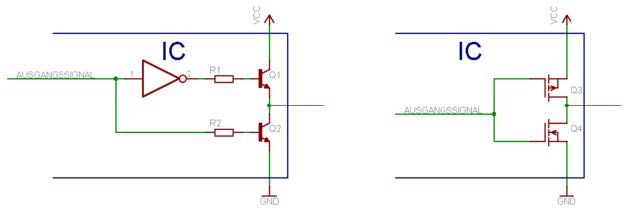
\epsfig{file=figures/PushPull.jpg,width=0.55\textwidth}\\
	  \caption{Push-pull output}
     \end{center}
\end{figure}
\os{\newpage}

\bi
	\ite \textbf{open drain} (open collector for bipolar transistors): only the transistor to GND exists
	\bi
		\ite the pin can only pull the line low; a resistor pulls it high
		\ite several outputs may share one line: it is low if any output pulls it low (``wired AND'')
		\ite the rising edge is slow, as the pull-up resistor charges the line capacitance ($\tau = RC$)
		\ite the high level may differ from the chip's supply (level shifting, e.g.\ 3.3\,V to 5\,V)
		\ite used for I$^2$C, interrupt lines, reset lines
	\ei
\ei
\begin{figure}[!hbtp]
     \begin{center}
	  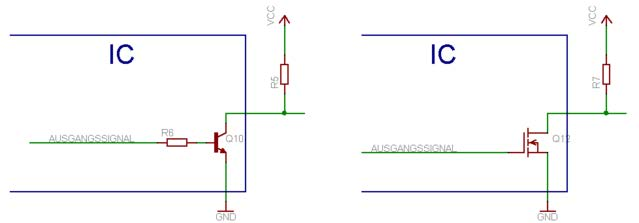
\epsfig{file=figures/OpenCollector.jpg,width=0.55\textwidth}\\
	  \caption{Open-drain output with external pull-up resistor}
     \end{center}
\end{figure}
\os{\newpage}

\bi
	\ite \textbf{tri-state}: a push-pull stage with an additional ``off'' state (high impedance, Z)
	\bi
		\ite in state Z the pin neither drives high nor low and behaves as if it were not connected
		\ite many devices can share a bus as long as only one of them drives at a time
		\ite on the RP2040: output enable = 0 means Z
		\ite open drain can be emulated: output value fixed at 0, switch only the output enable
	\ei
\ei
\begin{figure}[!hbtp]
     \begin{center}
	  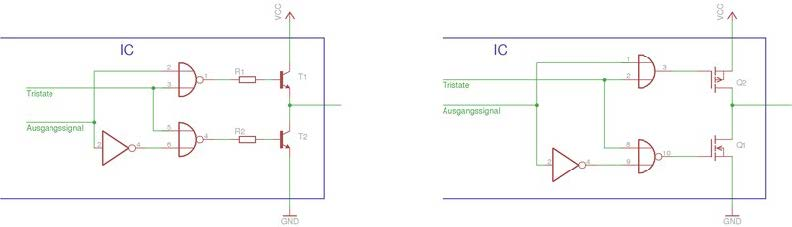
\epsfig{file=figures/TriState.jpg,width=0.55\textwidth}\\
	  \caption{Tri-state output}
     \end{center}
\end{figure}
\os{\newpage}

\item[{\rot\bf Inputs}]~\\[-3ex]
\bi
	\ite an unconnected (``floating'') input reads random values: it picks up noise
	\bi
		\ite always define the idle level with a pull-up or pull-down resistor
		\ite RP2040: internal pull-up / pull-down of about 50--80\,k$\Omega$ in the pad
	\ei
	\ite a typical button connects the pin to GND and uses the pull-up: \textbf{pressed = low}
	\ite \textbf{Schmitt trigger}: two switching thresholds (hysteresis), so a slowly changing or noisy signal gives one clean edge instead of many
	\ite electrical limits matter
	\bi
		\ite 3.3\,V maximum on any pin of the RP2040 -- a 5\,V signal needs a level shifter or voltage divider
		\ite drive strength 2, 4 (default), 8 or 12\,mA per pin -- enough for an LED, never for a motor or relay
	\ei
\ei
\os{\newpage}

\item[{\rot\bf Contact bounce}]~\\[-3ex]
\bi
	\ite mechanical contacts do not close cleanly: they bounce for some 100\,$\mu$s up to about 20\,ms
	\ite the software sees many edges for one press -- Wokwi simulates this as well
\ei
\begin{figure}[!hbtp]
\begin{center}
\resizebox{0.75\textwidth}{!}{%
\begin{tikztimingtable}[timing/slope=0.05, xscale=0.9, yscale=1.2, font=\sffamily\small]
	button (raw) & 4H 0.4L 0.3H 0.3L 0.2H 0.5L 0.15H 8L 0.2H 0.2L 0.3H 4H \\
	debounced    & 7.85H 8.7L 2H \\
\extracode
	\draw[decorate,decoration={brace,amplitude=4pt}] (4,0.4) -- node[above=4pt,font=\sffamily\scriptsize] {bounces} (5.85,0.4);
	\draw[<->] (5.85,-2.9) -- node[below,font=\sffamily\scriptsize] {stable for 20 ms} (7.85,-2.9);
\end{tikztimingtable}}
\caption{Bouncing button and debounced signal}
\end{center}
\end{figure}
\bi
	\ite hardware solution: RC low-pass filter followed by a Schmitt trigger
	\ite software solution: accept a new level only if it was stable for a certain time
\ei
\os{\newpage}

\item[{\rot\bf Debouncing in software (Rust)}]~\\[-3ex]
\begin{lstlisting}[language=Rust]
let mut led = pins.gpio15.into_push_pull_output();
// Button connects the pin to GND -> use the internal pull-up, pressed = low.
let mut button = pins.gpio14.into_pull_up_input();

let mut stable_pressed = false; // debounced state
let mut counter = 0; // how long the raw level differs from the stable state

loop {
    let raw_pressed = button.is_low().unwrap();
    if raw_pressed != stable_pressed {
        counter += 1;
        if counter >= STABLE_MS {
            stable_pressed = raw_pressed;
            counter = 0;
            if stable_pressed {
                led.toggle().unwrap(); // react on the press edge only
            }
        }
    } else {
        counter = 0;
    }
    delay.delay_ms(1); // sample every 1 ms
}
\end{lstlisting}
\bi
	\ite C version: \texttt{examples/interfaces/c/button\_debounce}
\ei
\os{\newpage}
\end{description}

%%%%%%%%%%%%%%%%%%%%%%%%%%%%%%%%%%%%%%%%%%%%%%%%%%%%%%%%%%%%%%%%%%%%%%%%%%%
\section{Interrupts}
%%%%%%%%%%%%%%%%%%%%%%%%%%%%%%%%%%%%%%%%%%%%%%%%%%%%%%%%%%%%%%%%%%%%%%%%%%%
\nsl{Polling a button every millisecond works, but it keeps the processor
busy and the reaction time depends on the loop. With an interrupt the
hardware itself watches the pin. When the selected edge occurs, the
processor finishes the current instruction, saves its state and jumps to
an interrupt service routine (ISR). Afterwards the interrupted program
continues as if nothing had happened. This is efficient, but it brings a
new class of errors. The ISR and the main program run ``at the same time''
from the program's point of view, so every variable they share must be
protected.}

\begin{description}
\item[{\rot\bf How an interrupt is handled on a Cortex-M}]~\\[-3ex]
\bi
	\ite the peripheral sets an interrupt flag (e.g.\ ``falling edge on GP14'')
	\ite if enabled, the request goes to the \textbf{NVIC} (nested vectored interrupt controller)
	\bi
		\ite RP2040: 32 interrupt lines per core, 4 priority levels
		\ite a higher priority interrupt can interrupt a running ISR (nesting)
	\ei
	\ite the core pushes registers onto the stack and loads the ISR address from the \textbf{vector table}
	\bi
		\ite latency on the Cortex-M0+: 15 clock cycles (120\,ns at 125\,MHz)
	\ei
	\ite the ISR must \textbf{clear the flag}, otherwise it is entered again immediately
	\ite on return the saved registers are restored automatically
\ei
\os{\newpage}

\item[{\rot\bf Rules for interrupt service routines}]~\\[-3ex]
\bi
	\ite keep ISRs \textbf{short}: set a flag, store a value, wake up a task
	\ite no blocking calls (delays, waiting for a UART, \texttt{printf}) inside an ISR
	\ite variables shared with the main program
	\bi
		\ite C: declare them \texttt{volatile}, so the compiler reads them from memory every time
		\ite \texttt{volatile} does \textbf{not} make an access atomic: a 64 bit value or a read-modify-write (\texttt{count++}) can still be interrupted in the middle
		\ite protect such accesses with a critical section (interrupts disabled for a short time)
	\ei
	\ite Rust enforces this: a \texttt{static} shared with an ISR must be wrapped, e.g.\ in a \texttt{Mutex} that can only be opened inside a critical section
\ei
\os{\newpage}

\item[{\rot\bf GPIO interrupt (C, Arduino API)}]~\\[-3ex]
\bi
	\ite try it: one press often gives several interrupts -- the bouncing is visible again
\ei
\begin{lstlisting}[language=C]
const int LED = 15, BUTTON = 14;
volatile uint32_t irqCount = 0;   // shared with the ISR -> volatile

void onButton() {                 // interrupt service routine: keep it short
  digitalWrite(LED, !digitalRead(LED));
  irqCount++;
}

void setup() {
  Serial1.begin(115200);
  pinMode(LED, OUTPUT);
  pinMode(BUTTON, INPUT_PULLUP);
  attachInterrupt(digitalPinToInterrupt(BUTTON), onButton, FALLING);
}
void loop() {
  static uint32_t last = 0;
  uint32_t now = irqCount;        // 32 bit read is atomic on the Cortex-M0+
  if (now != last) {
    Serial1.printf("interrupts so far: %lu\n", (unsigned long)now);
    last = now;
  }
}
\end{lstlisting}
\os{\newpage}

\item[{\rot\bf GPIO interrupt (Rust)}]~\\[-3ex]
\begin{lstlisting}[language=Rust]
// Hand-over main() -> ISR; the Mutex opens only in a critical section
static SHARED: Mutex<RefCell<Option<(LedPin, ButtonPin)>>> = Mutex::new(RefCell::new(None));

    let led = pins.gpio15.into_push_pull_output(); // in main()
    let button = pins.gpio14.into_pull_up_input();
    button.set_interrupt_enabled(EdgeLow, true);
    critical_section::with(|cs| SHARED.borrow(cs).replace(Some((led, button))));
    unsafe { pac::NVIC::unmask(pac::Interrupt::IO_IRQ_BANK0) };
    loop { cortex_m::asm::wfi(); } // sleep until an interrupt arrives

#[interrupt]
fn IO_IRQ_BANK0() {
    static mut PINS: Option<(LedPin, ButtonPin)> = None; // taken from SHARED once
    if PINS.is_none() {
        critical_section::with(|cs| *PINS = SHARED.borrow(cs).take());
    }
    if let Some((led, button)) = PINS {
        if button.interrupt_status(EdgeLow) {
            led.toggle().unwrap();
            button.clear_interrupt(EdgeLow); // otherwise the IRQ fires again at once
        }
    }
}
\end{lstlisting}
\os{\newpage}

\item[{\rot\bf Ownership across the interrupt boundary}]~\\[-3ex]
\bi
	\ite the pins are \textbf{moved} into the ISR: after the hand-over, \texttt{main()} cannot touch them any more
	\ite a data race between main program and ISR is therefore impossible -- the compiler rejects such code
	\ite the C version compiles even if both sides write \texttt{irqCount} without protection; the error shows up only now and then at run time
	\ite in larger programs a framework handles this hand-over, e.g.\ RTIC or Embassy (see chapter Operating Systems)
\ei
\os{\newpage}
\end{description}

%%%%%%%%%%%%%%%%%%%%%%%%%%%%%%%%%%%%%%%%%%%%%%%%%%%%%%%%%%%%%%%%%%%%%%%%%%%
\section{Timers, PWM and Watchdog}
%%%%%%%%%%%%%%%%%%%%%%%%%%%%%%%%%%%%%%%%%%%%%%%%%%%%%%%%%%%%%%%%%%%%%%%%%%%
\nsl{Almost every embedded application needs time: a periodic control
loop, a timeout, the frequency of a signal, the brightness of an LED. A
timer is basically a counter that is incremented by a known clock.
Comparing the counter with a value produces events at defined times
(output compare, PWM). Copying the counter at an external edge measures
the time of that edge (input capture). A special timer, the watchdog,
resets the system if the software stops working.}

\begin{description}
\item[{\rot\bf Building blocks of a timer}]~\\[-3ex]
\bi
	\ite \textbf{prescaler / divider}: reduces the input clock, e.g.\ 125\,MHz / 125 = 1\,MHz
	\ite \textbf{counter}: counts up (or down) with every divided clock
	\ite \textbf{top / reload value}: the counter wraps to 0 when it reaches it $\Rightarrow$ period
	\ite \textbf{compare} register: an event (interrupt or pin change) when counter = compare
	\ite \textbf{capture} register: the counter value is copied when an external edge arrives
	\bi
		\ite the difference of two captures gives period or pulse width with clock accuracy
	\ei
\ei
\bi
	\ite RP2040 timer: a 64 bit counter incremented every microsecond, 4 alarms (compare on the lower 32 bits) that raise interrupts
	\bi
		\ite \texttt{sleep\_ms()}, \texttt{delay()} and timeouts are built on it
		\ite 64 bit at 1\,MHz overflows after more than 500\,000 years
	\ei
\ei
\os{\newpage}

\item[{\rot\bf Pulse width modulation (PWM)}]~\\[-3ex]
\bi
	\ite a digital output switched periodically with a variable \textbf{duty cycle}
	\ite after averaging (LED + eye, motor + inertia, RC low-pass) the result behaves like an analog value
	\ite applications: LED brightness, DC motor speed, servo position, simple D/A conversion
\ei
\begin{figure}[!hbtp]
\begin{center}
\resizebox{0.75\textwidth}{!}{%
\begin{tikzpicture}[font=\sffamily\small,>=Stealth]
	% counter sawtooth
	\draw[->] (0,0) -- (10.5,0) node[right]{t};
	\draw[->] (0,0) -- (0,2.4) node[above]{counter};
	\foreach \x in {0,3.3,6.6} \draw[thick,blue] (\x,0) -- (\x+3.3,2) -- (\x+3.3,0);
	\draw[dashed] (0,2) node[left]{TOP} -- (10,2);
	\draw[dashed,red] (0,1.2) node[left]{CC} -- (10,1.2);
	% output
	\draw[->] (0,-3) -- (10.5,-3) node[right]{t};
	\node[left] at (0,-2.3) {output};
	\foreach \x in {0,3.3,6.6} {
		\draw[thick] (\x,-1.8) -- (\x+1.98,-1.8) -- (\x+1.98,-3) -- (\x+3.3,-3) -- (\x+3.3,-1.8);
		\draw[dotted] (\x+1.98,1.2) -- (\x+1.98,-1.8);
	}
	\draw[<->] (0,-3.4) -- node[below]{$T = (\mathrm{TOP}+1)\cdot \mathrm{DIV} / f_{sys}$} (3.3,-3.4);
	\draw[<->] (6.6,-1.5) -- node[above,font=\sffamily\scriptsize]{high while counter $<$ CC} (8.58,-1.5);
\end{tikzpicture}}
\caption{PWM: the output is high while the counter is below the compare value}
\end{center}
\end{figure}
\bi
	\ite duty cycle $= \mathrm{CC} / (\mathrm{TOP}+1)$, \quad $f_{PWM} = f_{sys} / (\mathrm{DIV}\cdot(\mathrm{TOP}+1))$
\ei
\os{\newpage}

\item[{\rot\bf PWM on the RP2040}]~\\[-3ex]
\bi
	\ite 8 slices, each with a 16 bit counter, a fractional divider (8.4 bit) and two outputs A and B
	\ite fixed mapping: GPIO $n$ $\rightarrow$ slice $(n/2) \bmod 8$, channel A for even, B for odd $n$
	\bi
		\ite GP15 $\rightarrow$ slice 7, channel B
	\ei
	\ite both channels of a slice share frequency, but have their own compare value (duty cycle)
	\ite phase-correct mode: count up and down -- symmetric pulses, half the frequency
	\ite channel B can also be an input: the counter then counts edges or measures the high time of an external signal
\ei
\os{\newpage}

\item[{\rot\bf PWM example: fading LED (C)}]~\\[-3ex]
\begin{lstlisting}[language=C]
// f_PWM = f_sys / (DIV * (TOP + 1)); with DIV = f_sys / 1 MHz -> 1 kHz
#include "hardware/clocks.h"
#include "hardware/pwm.h"

const uint LED = 15;
const uint16_t TOP = 999;
uint slice;

void setup() {
  gpio_set_function(LED, GPIO_FUNC_PWM);  // FUNCSEL = PWM
  slice = pwm_gpio_to_slice_num(LED);     // = 7
  uint32_t div = clock_get_hz(clk_sys) / 1000000;   // e.g. 125 or 200
  pwm_set_clkdiv_int_frac(slice, div, 0); // counter clock = 1 MHz
  pwm_set_wrap(slice, TOP);               // counts 0..TOP
  pwm_set_enabled(slice, true);
}

void loop() {
  for (int duty = 0; duty <= TOP; duty++) {        // fade in
    pwm_set_gpio_level(LED, duty);                  // duty = level / (TOP + 1)
    sleep_ms(1);
  }
  // ... fade out ...
}
\end{lstlisting}
\os{\newpage}

\item[{\rot\bf PWM example: fading LED (Rust)}]~\\[-3ex]
\begin{lstlisting}[language=Rust]
const TOP: u16 = 999;

let slices = hal::pwm::Slices::new(pac.PWM, &mut pac.RESETS);
let mut pwm = slices.pwm7;
pwm.set_div_int(125); // counter clock 125 MHz / 125 = 1 MHz
pwm.set_top(TOP); // counts 0..=999 -> period 1 ms
pwm.enable();

let channel = &mut pwm.channel_b;
channel.output_to(pins.gpio15); // FUNCSEL = PWM

loop {
    // Duty cycle = compare value / (TOP + 1)
    for duty in (0..=TOP).chain((0..=TOP).rev()) {
        channel.set_duty_cycle(duty).unwrap();
        delay.delay_us(1000);
    }
}
\end{lstlisting}
\bi
	\ite \texttt{set\_duty\_cycle()} comes from the \texttt{SetDutyCycle} trait of \texttt{embedded-hal}: drivers written against this trait work on every microcontroller with a HAL
	\ite look at LED\_PWM in the logic analyzer: 1\,kHz, changing pulse width
\ei
\os{\newpage}

\item[{\rot\bf Watchdog}]~\\[-3ex]
\bi
	\ite a counter that resets the whole chip when it expires
	\ite the software must restart (``feed'', ``kick'') it regularly
	\ite if the program hangs in an endless loop or a deadlock, the feeding stops and the system restarts in a defined state
	\ite rules
	\bi
		\ite feed it at \textbf{one} place in the main loop -- never from a timer interrupt (that keeps running when the main loop hangs)
		\ite check the reset reason at start-up and log or report watchdog resets
		\ite pause it while the debugger halts the CPU
	\ei
	\ite RP2040: maximum timeout about 8.3\,s; register \texttt{WATCHDOG\_REASON} tells whether the last reset came from the watchdog
\ei
\os{\newpage}

\item[{\rot\bf Watchdog example (Rust)}]~\\[-3ex]
\begin{lstlisting}[language=Rust]
// Read the reset reason before the HAL takes the WATCHDOG peripheral.
let by_watchdog = pac.WATCHDOG.reason().read().timer().bit_is_set();
let mut watchdog = hal::Watchdog::new(pac.WATCHDOG);
// ... clocks, pins, UART ...
if by_watchdog {
    writeln!(uart, "Restarted by the WATCHDOG\r").unwrap();
} else {
    writeln!(uart, "Power-on reset\r").unwrap();
}

watchdog.pause_on_debug(true); // do not reset while halted in the debugger
watchdog.start(1_000.millis()); // timeout 1 s

loop {
    while button.is_low().unwrap() {
        // simulated "hang": the watchdog is no longer fed
    }
    watchdog.feed();
    led.toggle().unwrap();
    delay.delay_ms(100);
}
\end{lstlisting}
\bi
	\ite hold the button for more than one second and watch the serial monitor
	\ite C version: \texttt{watchdog\_enable()}, \texttt{watchdog\_update()}, \texttt{watchdog\_caused\_reboot()}
\ei
\os{\newpage}
\end{description}

%%%%%%%%%%%%%%%%%%%%%%%%%%%%%%%%%%%%%%%%%%%%%%%%%%%%%%%%%%%%%%%%%%%%%%%%%%%
\section{Analog Input (ADC)}
%%%%%%%%%%%%%%%%%%%%%%%%%%%%%%%%%%%%%%%%%%%%%%%%%%%%%%%%%%%%%%%%%%%%%%%%%%%
\nsl{Sensors often deliver a voltage: a potentiometer, a thermistor in a
voltage divider, a microphone amplifier. An analog-to-digital converter
(ADC) turns this voltage into a number. Two parameters describe it: the
resolution (how many steps) and the sampling rate (how many conversions
per second). The datasheet value for the resolution is an upper bound;
noise and non-linearity reduce the effective number of bits.}

\begin{description}
\item[{\rot\bf Principle and key figures}]~\\[-3ex]
\bi
	\ite \textbf{successive approximation} (SAR): the converter compares the input with the output of an internal D/A converter and determines one bit per step, starting with the MSB -- $n$ steps for $n$ bits
	\ite \textbf{resolution}: $n$ bit $\Rightarrow$ $2^n$ steps; one step (LSB) $= V_{ref} / 2^n$
	\bi
		\ite RP2040: 12 bit, $V_{ref} = 3.3$\,V $\Rightarrow$ 1\,LSB $\approx 0.8$\,mV
		\ite effective resolution (ENOB) is lower, about 9 bit
	\ei
	\ite \textbf{sampling rate}: RP2040 up to 500\,000 samples/s (96 cycles of the 48\,MHz ADC clock)
	\bi
		\ite sampling theorem: the signal must not contain frequencies above half the sampling rate, otherwise they appear as wrong low frequencies (aliasing) $\Rightarrow$ analog low-pass filter before the ADC
	\ei
	\ite one converter, an input \textbf{multiplexer} selects the channel
	\bi
		\ite channels 0--3 = GP26--GP29, channel 4 = internal temperature sensor
	\ei
\ei
\os{\newpage}

\item[{\rot\bf ADC example: potentiometer and chip temperature (C)}]~\\[-3ex]
\begin{lstlisting}[language=C]
#include "hardware/adc.h"

void setup() {
  Serial1.begin(115200);           // UART0, 8N1
  adc_init();
  adc_gpio_init(26);               // disable digital input buffer on GP26
  adc_set_temp_sensor_enabled(true);
}

void loop() {
  adc_select_input(0);             // multiplexer -> channel 0 (GP26)
  uint16_t raw = adc_read();       // 12 bit: 0 .. 4095
  uint32_t millivolt = raw * 3300u / 4095u;

  adc_select_input(4);             // channel 4 = temperature sensor
  float vSense = adc_read() * 3.3f / 4095.0f;
  float celsius = 27.0f - (vSense - 0.706f) / 0.001721f;   // datasheet formula

  Serial1.printf("ADC0 = %4u (%4lu mV)   chip temperature = %.1f C\n",
                 raw, (unsigned long)millivolt, celsius);
  sleep_ms(500);
}
\end{lstlisting}
\bi
	\ite turn the potentiometer in Wokwi and watch the values; Rust version: \texttt{adc\_uart.rs}
\ei
\os{\newpage}
\end{description}

%%%%%%%%%%%%%%%%%%%%%%%%%%%%%%%%%%%%%%%%%%%%%%%%%%%%%%%%%%%%%%%%%%%%%%%%%%%
\section{Serial Interfaces}
%%%%%%%%%%%%%%%%%%%%%%%%%%%%%%%%%%%%%%%%%%%%%%%%%%%%%%%%%%%%%%%%%%%%%%%%%%%
\nsl{Sending data bit by bit over a few wires saves pins, cable and board
space, so nearly all communication between chips and devices is serial.
Three interfaces dominate on the board level. The UART is asynchronous
and point-to-point and is used for consoles, GPS receivers and radio
modules. I$^2$C is a two-wire bus with addresses, used for slow sensors and
configuration. SPI is a fast synchronous interface with a separate select
line per device, used for displays, memories and converters. They differ
in how the receiver knows when to sample a bit: an agreed baud rate
(UART) or a separate clock line (I$^2$C, SPI).}

\begin{description}
\item[{\rot\bf Overview}]~\\[-3ex]
\begin{center}
\resizebox{\textwidth}{!}{%
\begin{tabular}{|l|c|c|c|}
\hline
 & \textbf{UART} & \textbf{I$^2$C} & \textbf{SPI} \\
\hline
clock & none (agreed baud rate) & SCL from controller & SCK from controller \\
wires & TX, RX (+ GND) & SDA, SCL (+ GND) & SCK, COPI, CIPO, CS per device \\
topology & point-to-point & bus, 7 bit addresses & bus, chip select lines \\
direction & full duplex & half duplex & full duplex \\
typical speed & 9.6 k -- 1 Mbit/s & 100 k, 400 k, 1 Mbit/s & 1 -- 50 Mbit/s \\
typical use & console, GPS, modems & sensors, EEPROM, RTC & displays, flash, SD card \\
\hline
\end{tabular}}
\end{center}
\bi
	\ite ``controller'' and ``peripheral'' (or ``target'') replace the older terms master and slave; for SPI the data lines are called COPI (controller out, peripheral in) and CIPO -- older documents use MOSI and MISO
\ei
\os{\newpage}

\item[{\rot\bf UART: asynchronous serial transmission}]~\\[-3ex]
\bi
	\ite idle line is high; a frame starts with a \textbf{start bit} (low)
	\ite then 5--9 data bits, \textbf{LSB first}, optional parity bit, 1 or 2 \textbf{stop bits} (high)
	\ite both sides must use the same settings, e.g.\ ``115200 8N1'' = 115200 bit/s, 8 data bits, no parity, 1 stop bit
	\ite the receiver synchronises on the falling edge of the start bit and samples each bit in its middle (oversampling with 16 times the baud rate)
	\bi
		\ite clocks may differ by a few percent before the last bit is sampled wrongly
	\ei
\ei
\begin{figure}[!hbtp]
\begin{center}
\resizebox{0.9\textwidth}{!}{%
\begin{tikztimingtable}[timing/slope=0.05, xscale=2.2, yscale=1.5, font=\sffamily\small]
	TX & 2H L D{1} D{0} D{0} D{0} D{0} D{0} D{1} D{0} H 2H \\
\extracode
	\begin{scope}[font=\sffamily\scriptsize]
	\node[above] at (1,1.1) {idle};
	\node[above] at (2.5,1.1) {start};
	\foreach \i in {0,...,7} \node[above] at (3.5+\i,1.1) {D\i};
	\node[above] at (11.5,1.1) {stop};
	\end{scope}
\end{tikztimingtable}}
\caption{UART frame 8N1 for the character 'A' (0x41 = 0100\,0001, sent LSB first)}
\end{center}
\end{figure}
\os{\newpage}

\item[{\rot\bf UART: errors and signal levels}]~\\[-3ex]
\bi
	\ite error detection in the receiver
	\bi
		\ite \textbf{parity error}: number of 1 bits does not match (detects single bit errors only)
		\ite \textbf{framing error}: stop bit is not high -- wrong baud rate or disturbed line
		\ite \textbf{overrun}: new data arrived before the software read the old data
	\ei
	\ite the UART defines the frame, not the voltages
	\bi
		\ite \textbf{TTL / CMOS level}: 0\,V / 3.3\,V directly at the chip pins, a few centimetres to metres
		\ite \textbf{RS-232}: $\pm 3$ to $\pm 15$\,V, inverted, point-to-point, up to about 15\,m
		\ite \textbf{RS-485}: differential pair, up to 1200\,m, several devices on one bus (Modbus, DMX)
		\ite \textbf{USB-to-UART} bridges (CP2102, FT232, CH340): the usual way to a PC today
	\ei
	\ite RP2040: 2 UARTs (ARM PL011) with 32 byte FIFOs for transmit and receive
\ei
\os{\newpage}

\item[{\rot\bf UART example: echo in upper case}]~\\[-3ex]
\begin{lstlisting}[language=C]
#include <ctype.h>
#include "hardware/uart.h"

void setup() {
  uart_init(uart0, 115200);                 // 8N1 is the default format
  gpio_set_function(0, GPIO_FUNC_UART);     // GP0 = TX
  gpio_set_function(1, GPIO_FUNC_UART);     // GP1 = RX
  uart_puts(uart0, "UART echo ready\r\n");
}

void loop() {
  if (uart_is_readable(uart0)) {            // RX FIFO not empty?
    char c = uart_getc(uart0);
    uart_putc_raw(uart0, toupper(c));
  }
}
\end{lstlisting}
\begin{lstlisting}[language=Rust]
let mut uart = UartPeripheral::new(pac.UART0, uart_pins, &mut pac.RESETS)
    .enable(
        UartConfig::new(115_200.Hz(), DataBits::Eight, None, StopBits::One),
        clocks.peripheral_clock.freq(),
    )
    .unwrap();
loop {
    // block!() polls the non-blocking read until a byte has arrived
    let byte = block!(uart.read()).unwrap();
    block!(uart.write(byte.to_ascii_uppercase())).unwrap();
}
\end{lstlisting}
\os{\newpage}

\item[{\rot\bf I$^2$C: a two-wire bus}]~\\[-3ex]
\bi
	\ite two open-drain lines with pull-up resistors: SDA (data) and SCL (clock)
	\ite the controller generates the clock and starts every transfer
	\ite each peripheral has a 7 bit address (some 10 bit), e.g.\ MPU6050 = 0x68
	\ite open drain makes the bus safe: nobody drives high, so two devices can never short the line
	\ite speeds: standard mode 100\,kbit/s, fast mode 400\,kbit/s, fast mode plus 1\,Mbit/s
	\ite typical pull-ups: 4.7\,k$\Omega$ at 100\,kHz, 2.2\,k$\Omega$ at 400\,kHz (the bus capacitance limits the rise time)
\ei
\os{\newpage}
\begin{figure}[!hbtp]
\begin{center}
\resizebox{0.8\textwidth}{!}{%
\begin{tikzpicture}[font=\sffamily\small,
	box/.style={draw,thick,minimum height=10mm,minimum width=22mm,align=center}]
	\draw[thick] (0,0) -- (11,0) node[right]{SCL};
	\draw[thick] (0,0.6) -- (11,0.6) node[right]{SDA};
	\node[box,fill=blue!10] (c) at (1.2,-1.6) {controller\\RP2040};
	\node[box,fill=orange!15] (p1) at (4.6,-1.6) {MPU6050\\0x68};
	\node[box,fill=orange!15] (p2) at (7.4,-1.6) {OLED display\\0x3C};
	\node[box,fill=orange!15] (p3) at (10.2,-1.6) {EEPROM\\0x50};
	\foreach \n in {c,p1,p2,p3} {
		\draw ($(\n.north)+(-0.3,0)$) -- ++(0,1.1) node[circle,fill,inner sep=1pt]{};
		\draw ($(\n.north)+(0.3,0)$) -- ++(0,2.1-0.4) node[circle,fill,inner sep=1pt]{};
	}
	\draw (0.3,0) -- (0.3,1.4) node[draw,minimum width=2mm,minimum height=7mm,anchor=south] (r1) {};
	\draw (0.8,0.6) -- (0.8,1.4) node[draw,minimum width=2mm,minimum height=7mm,anchor=south] (r2) {};
	\draw (r1.north) -- ++(0,0.3) -| (r2.north);
	\node[above] at (0.55,2.4) {3.3\,V};
	\node[left,font=\sffamily\scriptsize] at (0.2,1.75) {$R_P$};
\end{tikzpicture}}
\caption{I$^2$C bus: all devices share SDA and SCL, pull-up resistors $R_P$ define the high level}
\end{center}
\end{figure}
\os{\newpage}

\item[{\rot\bf I$^2$C: protocol}]~\\[-3ex]
\bi
	\ite SDA may only change while SCL is low -- with two exceptions
	\bi
		\ite \textbf{START}: SDA falls while SCL is high
		\ite \textbf{STOP}: SDA rises while SCL is high
	\ei
	\ite after START: 7 bit address + R/$\overline{\mbox{W}}$ bit (0 = write, 1 = read)
	\ite every byte is followed by an \textbf{acknowledge} bit: the receiver pulls SDA low (ACK) or leaves it high (NACK)
	\ite a peripheral may hold SCL low to make the controller wait (\textbf{clock stretching})
\ei
\begin{figure}[!hbtp]
\begin{center}
\resizebox{0.9\textwidth}{!}{%
\begin{tikztimingtable}[timing/slope=0.1, xscale=2.4, yscale=1.6, font=\sffamily\small]
	SCL & 2.5H 18{0.5L 0.5H} 0.5L 2.5H \\
	SDA & 2H 0.5L D{1} D{1} D{0} D{1} D{0} D{0} D{0} D{0} L 8D{data byte} L 0.75L 2.25H \\
\extracode
	\begin{scope}[font=\sffamily\scriptsize]
	\node[above] at (2.2,1.1)  {START};
	\node[above] at (6,1.1)    {address 0x68};
	\node[above] at (10,1.1)   {W};
	\node[above] at (11,1.1)   {ACK};
	\node[above] at (15.5,1.1) {data};
	\node[above] at (20,1.1)   {ACK};
	\node[above] at (21.6,1.1) {STOP};
	\end{scope}
\end{tikztimingtable}}
\caption{I$^2$C write: START, address 0x68 with R/$\overline{\mbox{W}}$ = 0, ACK, data byte, ACK, STOP}
\end{center}
\end{figure}
\os{\newpage}

\item[{\rot\bf Reading a sensor register over I$^2$C}]~\\[-3ex]
\bi
	\ite sensors are organised as a set of registers with an 8 bit register address
	\ite reading a register is a combined transfer
	\bi
		\ite START, address + W, \textbf{register address}
		\ite repeated START (no STOP in between, so no other controller can interfere), address + R
		\ite read one or more bytes; the controller ACKs every byte except the last one (NACK), then STOP
	\ei
	\ite most sensors increment the register address automatically: one transfer reads a whole block (``burst read'')
\ei
\begin{lstlisting}[language=C]
// Register read: write the register address without STOP,
// then read with a repeated START.
void readRegs(uint8_t reg, uint8_t *buf, size_t len) {
  i2c_write_blocking(i2c0, MPU6050, &reg, 1, true);   // true = no STOP
  i2c_read_blocking(i2c0, MPU6050, buf, len, false);
}
\end{lstlisting}
\os{\newpage}

\item[{\rot\bf I$^2$C example: MPU6050 acceleration sensor (Rust)}]~\\[-3ex]
\begin{lstlisting}[language=Rust]
// I2C lines are open drain: the pins need pull-up resistors.
let sda = pins.gpio4.reconfigure::<gpio::FunctionI2C, gpio::PullUp>();
let scl = pins.gpio5.reconfigure::<gpio::FunctionI2C, gpio::PullUp>();
let mut i2c = hal::I2C::i2c0(
    pac.I2C0, sda, scl, 400.kHz(), // fast mode
    &mut pac.RESETS, clocks.system_clock.freq(),
);

// Register read = write the register address, then (repeated start) read.
let mut id = [0u8; 1];
i2c.write_read(MPU6050, &[REG_WHO_AM_I], &mut id).unwrap();
writeln!(uart, "WHO_AM_I = 0x{:02X}\r", id[0]).unwrap();

// Leave sleep mode: write 0 to PWR_MGMT_1.
i2c.write(MPU6050, &[REG_PWR_MGMT_1, 0x00]).unwrap();

loop {
    // Burst read: 6 bytes from ACCEL_XOUT_H (X, Y, Z as big endian i16).
    let mut buf = [0u8; 6];
    i2c.write_read(MPU6050, &[REG_ACCEL_XOUT_H], &mut buf).unwrap();
    // ... convert: +-2 g range -> 16384 LSB per g ...
}
\end{lstlisting}
\bi
	\ite \texttt{write\_read()} is the repeated-start transfer from the previous slide (trait \texttt{embedded\_hal::i2c::I2c})
	\ite change the acceleration in Wokwi (click on the sensor) and compare SDA/SCL in the logic analyzer
\ei
\os{\newpage}

\item[{\rot\bf SPI: Serial Peripheral Interface}]~\\[-3ex]
\bi
	\ite synchronous, full duplex: with every clock one bit goes out on COPI and one comes in on CIPO
	\ite internally two shift registers that exchange their contents
	\ite each peripheral has its own \textbf{chip select} (CS, active low); only the selected one drives CIPO
	\ite push-pull lines and no addressing: much faster than I$^2$C, but one extra wire per device
	\ite no acknowledge, no standard for frame length or commands -- each device defines its own protocol in the datasheet
\ei
\begin{figure}[!hbtp]
\begin{center}
\resizebox{0.7\textwidth}{!}{%
\begin{tikzpicture}[font=\sffamily\small,>=Stealth,
	box/.style={draw,thick,minimum width=22mm,minimum height=12mm,align=center}]
	\node[box,fill=blue!10,minimum height=26mm] (c) at (0,0) {controller};
	\node[box,fill=orange!15] (p1) at (4.5,-2.6) {peripheral 1};
	\node[box,fill=orange!15] (p2) at (8,-2.6) {peripheral 2};
	% shared lines
	\foreach \y/\n in {1.0/SCK,0.6/COPI,0.2/CIPO} {
		\draw[thick] (1.1,\y) -- (9.6,\y) node[right,font=\sffamily\scriptsize]{\n};
	}
	% taps: peripheral tops are at y = -2.0
	\foreach \x in {4.5,8} {
		\draw[->,thick] (\x-0.75,1.0) -- (\x-0.75,-2.0);   \fill (\x-0.75,1.0) circle (1.5pt);
		\draw[->,thick] (\x-0.35,0.6) -- (\x-0.35,-2.0);   \fill (\x-0.35,0.6) circle (1.5pt);
		\draw[<-,thick] (\x+0.05,0.2) -- (\x+0.05,-2.0);   \fill (\x+0.05,0.2) circle (1.5pt);
	}
	% chip selects
	\draw[->,thick] (1.1,-0.4) node[above right,font=\sffamily\scriptsize]{CS1} -| ($(p1.north)+(0.6,0)$);
	\draw[->,thick] (1.1,-0.9) node[below right,font=\sffamily\scriptsize]{CS2} -| ($(p2.north)+(0.6,0)$);
\end{tikzpicture}}
\caption{SPI bus with two peripherals: shared clock and data lines, one chip select each}
\end{center}
\end{figure}
\os{\newpage}

\item[{\rot\bf SPI modes}]~\\[-3ex]
\bi
	\ite two settings define the timing; controller and peripheral must agree
	\bi
		\ite \textbf{CPOL}: idle level of the clock (0 = low, 1 = high)
		\ite \textbf{CPHA}: sample on the first (0) or second (1) clock edge
	\ei
\ei
\begin{center}
\begin{tabular}{|c|c|c|l|}
\hline
\textbf{mode} & \textbf{CPOL} & \textbf{CPHA} & \textbf{data sampled on} \\
\hline
0 & 0 & 0 & rising edge \\
1 & 0 & 1 & falling edge \\
2 & 1 & 0 & falling edge \\
3 & 1 & 1 & rising edge \\
\hline
\end{tabular}
\end{center}
\begin{figure}[!hbtp]
\begin{center}
\resizebox{0.75\textwidth}{!}{%
\begin{tikztimingtable}[timing/slope=0.1, xscale=1.3, yscale=1.4, font=\sffamily\small]
	CS   & 1H 18L 1H \\
	SCK  & 1L 8{L H} 2L 1L \\
	COPI & 1Z 2D{b7} 2D{b6} 2D{b5} 2D{b4} 2D{b3} 2D{b2} 2D{b1} 2D{b0} 2Z 1Z \\
\extracode
	\begin{pgfonlayer}{background}
	\foreach \x in {2,4,...,16} \draw[help lines,dashed] (\x,1) -- (\x,-5.2);
	\end{pgfonlayer}
\end{tikztimingtable}}
\caption{SPI mode 0: data changes on the falling edge and is sampled on the rising edge (dashed), MSB first}
\end{center}
\end{figure}
\os{\newpage}

\item[{\rot\bf SPI example: 74HC595 shift register}]~\\[-3ex]
\bi
	\ite the 74HC595 is a simple SPI-like device: 8 bit shift register (DS = data, SHCP = clock) plus an output latch (STCP)
	\ite a rising edge on STCP copies the shifted byte to the outputs Q0--Q7 -- classic way to get more output pins
\ei
\begin{lstlisting}[language=C]
#include "hardware/spi.h"

const uint PIN_SCK = 18, PIN_COPI = 19, PIN_LATCH = 17;

void setup() {
  spi_init(spi0, 1000 * 1000);              // 1 MHz
  spi_set_format(spi0, 8, SPI_CPOL_0, SPI_CPHA_0, SPI_MSB_FIRST);   // mode 0
  gpio_set_function(PIN_SCK, GPIO_FUNC_SPI);
  gpio_set_function(PIN_COPI, GPIO_FUNC_SPI);
  gpio_init(PIN_LATCH);
  gpio_set_dir(PIN_LATCH, GPIO_OUT);
}

void show(uint8_t pattern) {
  spi_write_blocking(spi0, &pattern, 1);    // 8 clocks shift the byte in
  gpio_put(PIN_LATCH, 1);                   // rising edge on STCP copies the
  gpio_put(PIN_LATCH, 0);                   // shift register to the outputs
}
\end{lstlisting}
\bi
	\ite Rust version: \texttt{spi\_shift\_register.rs} -- \texttt{spi.write()} followed by \texttt{spi.flush()}, which waits until the last bit has left the FIFO before the latch pulse
\ei
\os{\newpage}

\item[{\rot\bf Interfaces beyond the board}]~\\[-3ex]
\bi
	\ite \textbf{USB}: differential pair, host-controlled, up to 12\,Mbit/s on the RP2040 (full speed)
	\bi
		\ite device classes avoid special drivers: CDC (virtual serial port), HID (keyboard, mouse), MSC (mass storage)
		\ite the RP2040 boot ROM appears as a USB drive -- copy a \texttt{.uf2} file to flash it
	\ei
	\ite \textbf{CAN}: differential two-wire bus for cars and industrial machines
	\bi
		\ite multi-controller: all nodes may send; the message identifier decides by bitwise arbitration (a ``dominant'' 0 wins over a ``recessive'' 1), so the most important message always gets through without collisions
		\ite classic CAN 1\,Mbit/s, CAN FD up to 8\,Mbit/s in the data phase
		\ite the RP2040 has no CAN controller: use an external one (MCP2515 via SPI) or emulate it with PIO
	\ei
	\ite \textbf{PIO} (RP2040 specific): small state machines that execute their own I/O programs -- for protocols that have no hardware block (WS2812 LEDs, VGA, extra UARTs, CAN)
\ei
\os{\newpage}

\item[{\rot\bf Looking at the signals: the logic analyzer}]~\\[-3ex]
\bi
	\ite the Wokwi logic analyzer records up to 8 digital signals during the simulation
	\ite stop the simulation $\rightarrow$ the recording is downloaded as a VCD file (value change dump)
	\ite open it in PulseView (sigrok) or GTKWave
	\bi
		\ite PulseView has \textbf{protocol decoders}: UART, I$^2$C and SPI are shown as bytes, addresses, ACK/NACK
	\ei
	\ite this is the same work flow as with a real logic analyzer on real hardware -- and the most efficient way to find errors in serial communication
\ei
\os{\newpage}

\item[{\rot\bf Exercises}]~\\[-3ex]
\bi
	\ite GPIO: change \texttt{gpio\_blink\_registers} so that the LED is switched with GPIO\_OUT\_SET and GPIO\_OUT\_CLR. Then try to call \texttt{set\_high()} on an input pin in Rust and read the compiler message.
	\ite Interrupts: count the interrupts of one button press with bouncing enabled and disabled (attribute \texttt{"bounce": "0"} in \texttt{diagram.json}). Debounce in the ISR using the timer: ignore edges within 20\,ms of the last accepted one.
	\ite PWM: use the potentiometer (ADC) to set the LED brightness. Which PWM frequency is needed so that the LED does not flicker?
	\ite UART: record ``A'' in the logic analyzer, measure the bit time and compare with 1/115200\,s.
	\ite I$^2$C: decode one register read of the MPU6050 in PulseView and mark START, address, ACK, repeated START and NACK.
	\ite SPI: change the 74HC595 example to SPI mode 3. What happens and why?
\ei
\end{description}


%%%%%%%%%%%%%%%%%%%%%%%%%%%%%%%%%%%%%%%%%%%%%%%%%%%%%%%%%%%%%%%%%%%%%%%%%%
\chapter{TCP/IP and Serial Bus}


\section{The OSI 7 layer model }

\begin{description}



\os{newpage} item[{\rot\bf  Structure }]~\\[-3ex]

\bi
  \ite General

  \ite The 7 layers

  \ite Their tasks listed individually

  \ite Communication between the layers

  \ite Sources

\ei


\os{newpage} item[{\rot\bf  General }]~\\[-3ex]

\bi
  \ite Developed since 1979 \& standardised by ISO (International Organisation for Standardisation)

  \ite It consists of individual open layers

  \ite Serves the communication of information-processing systems as the basis for a number of manufacturerindependent network protocols.

\ei


\os{newpage} item[{\rot\bf  General }]~\\[-3ex]

\bi
  \ite Describes a unified procedure and rules for the exchange of data

  \ite Finds application in public communication technology

  \ite It is more or less a translation programme for data transfer between different systems.

\ei


\os{newpage} item[{\rot\bf  General }]~\\[-3ex]

\bi
  \ite Is hierarchically structured

  \ite Lower layer provides its services to the one above it

\ei


\os{newpage} item[{\rot\bf  The 7 layers }]~\\[-3ex]

\bi
  \ite From top to bottom

  \ite
  \begin{enumerate}
    \setcounter{enumii}{6}
    \ite application layer
  \end{enumerate}
  \ite
  \begin{enumerate}
    \setcounter{enumii}{5}
    \ite presentation layer
  \end{enumerate}
  \ite
  \begin{enumerate}
    \setcounter{enumii}{4}
    \ite session layer
  \end{enumerate}
  \ite
  \begin{enumerate}
    \setcounter{enumii}{3}
    \ite transport layer
  \end{enumerate}
  \ite
  \begin{enumerate}
    \setcounter{enumii}{2}
    \ite network layer (network layer)
  \end{enumerate}
  \ite
  \begin{enumerate}
    \setcounter{enumii}{1}
    \ite data link layer
  \end{enumerate}
  \ite
  \begin{enumerate}
    \ite physical layer (bit transmission layer)
  \end{enumerate}
\ei


\os{newpage} item[{\rot\bf  The 7 layers }]~\\[-3ex]

\bi
  \ite Layers 1-4 are assigned to the transport function

  \ite Layers 5 - 7 are assigned to the user functions

\ei



\os{newpage} item[{\rot\bf  The OSI Model (Open Systems Interconnection) }]~\\[-3ex]

\begin{center}
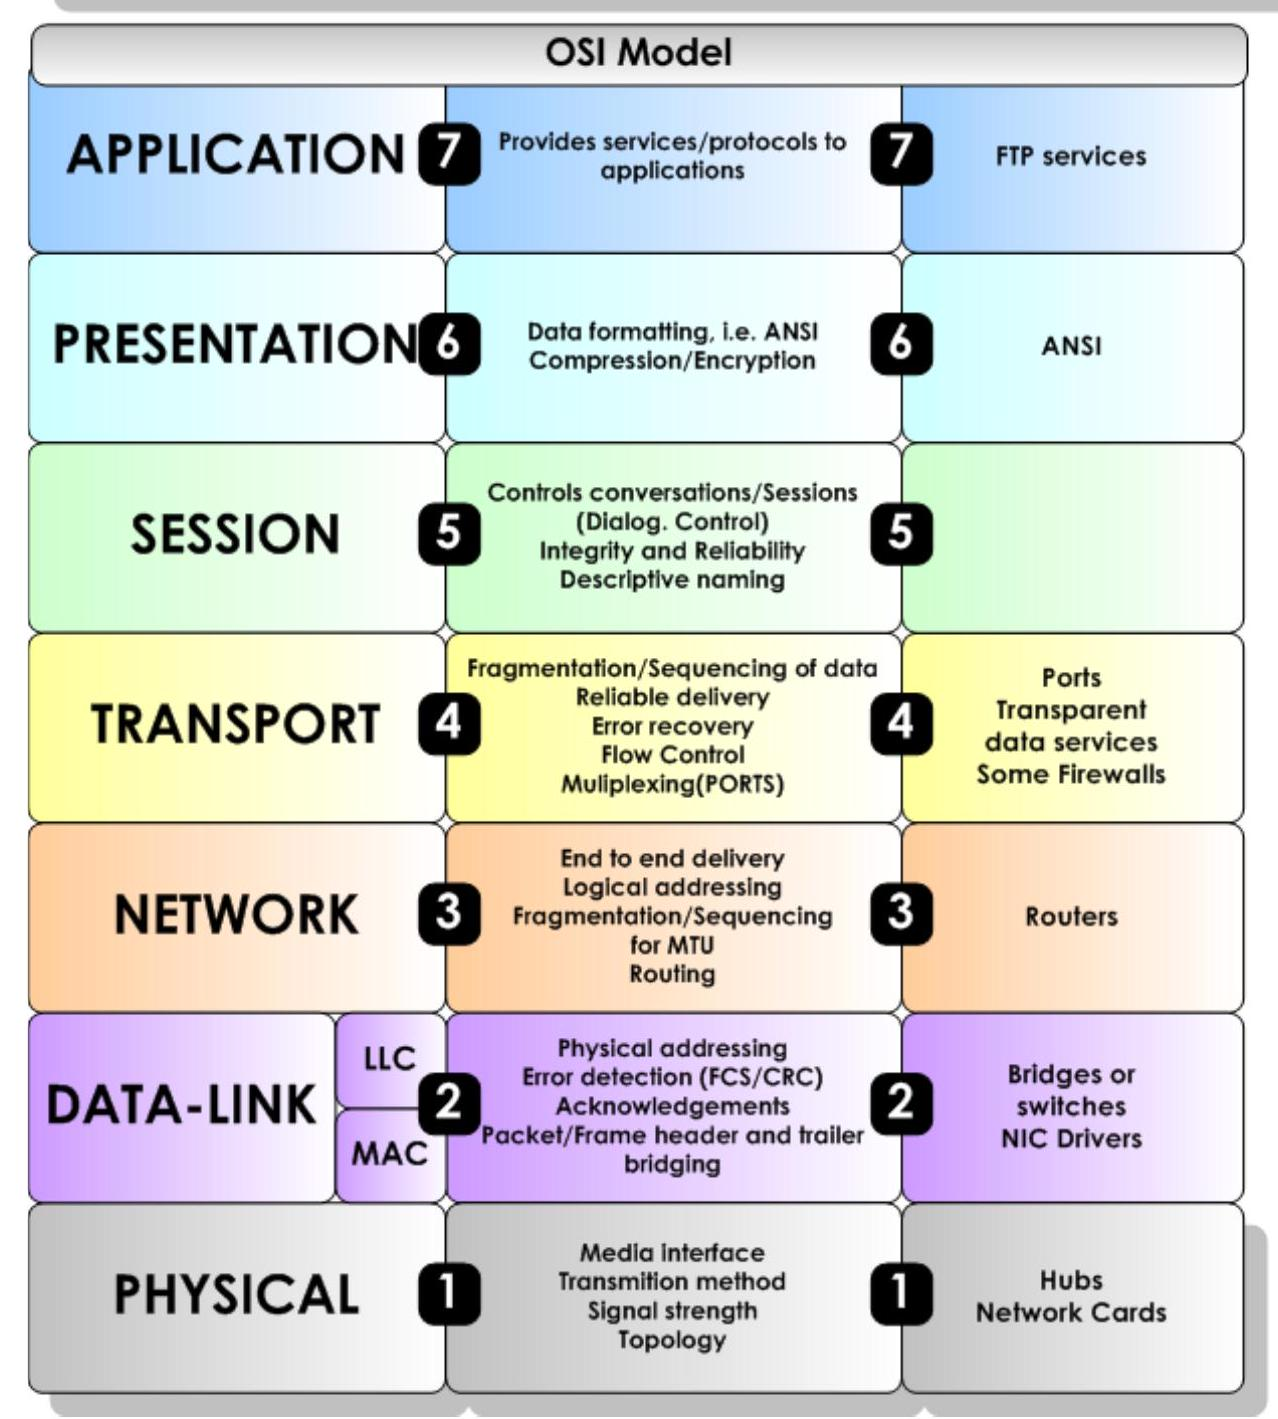
\includegraphics[max width=\textwidth]{2023_01_13_b07e3b4bcffdaab9792bg-009}
\end{center}

\begin{center}

\includegraphics[max width=\textwidth]{2023_01_13_b07e3b4bcffdaab9792bg-009(1)}
\end{center}

\begin{center}
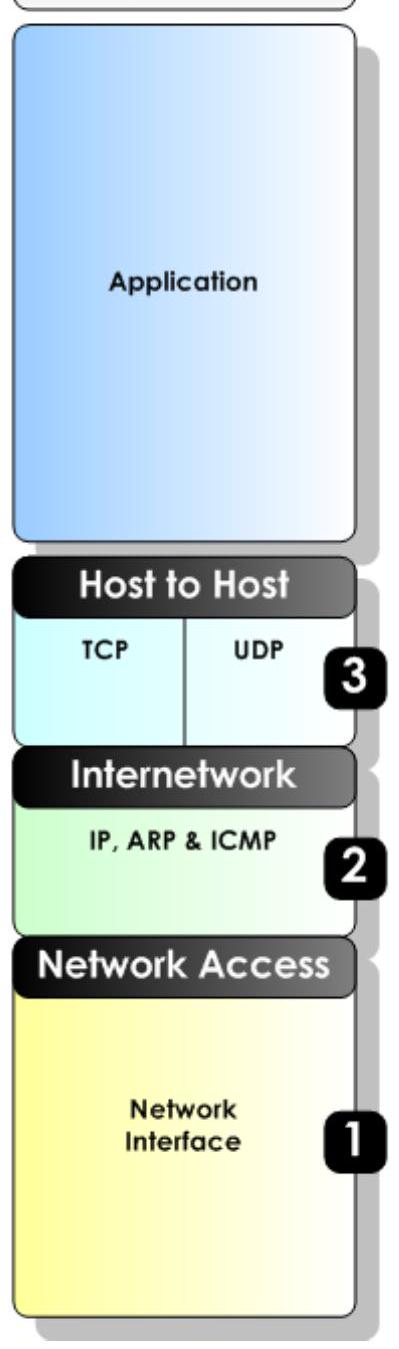
\includegraphics[max width=\textwidth]{2023_01_13_b07e3b4bcffdaab9792bg-009(2)}
\end{center}

(c) Copyright 2008 Steven Iveson WWW. \href{http://networkstuff.eu}{networkstuff.eu}

\begin{center}
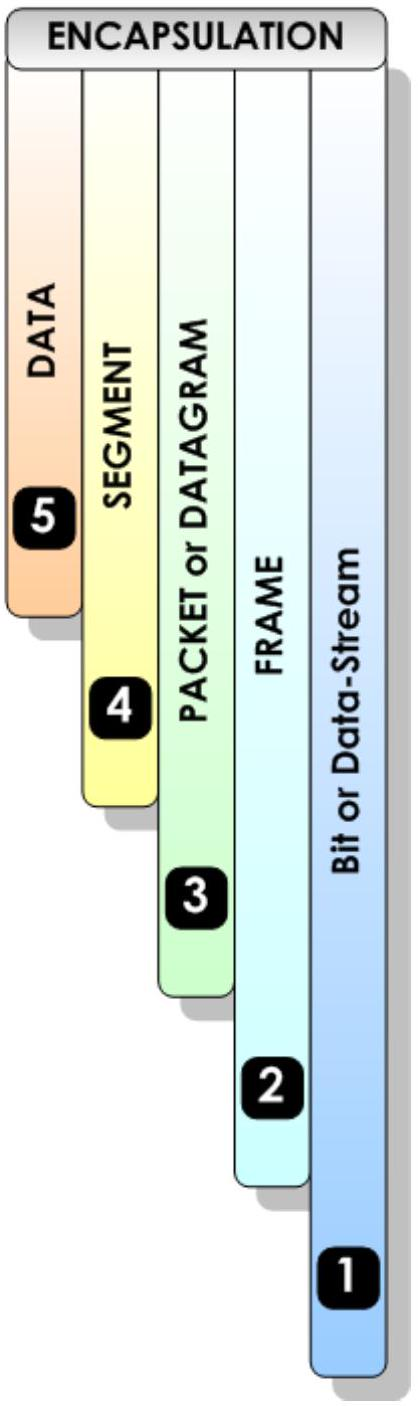
\includegraphics[max width=\textwidth]{2023_01_13_b07e3b4bcffdaab9792bg-009(3)}
\end{center}


\os{newpage} item[{\rot\bf  Reference Models }]~\\[-3ex]

Layer

Name of unit exchanged

The OSI reference model.

\begin{center}
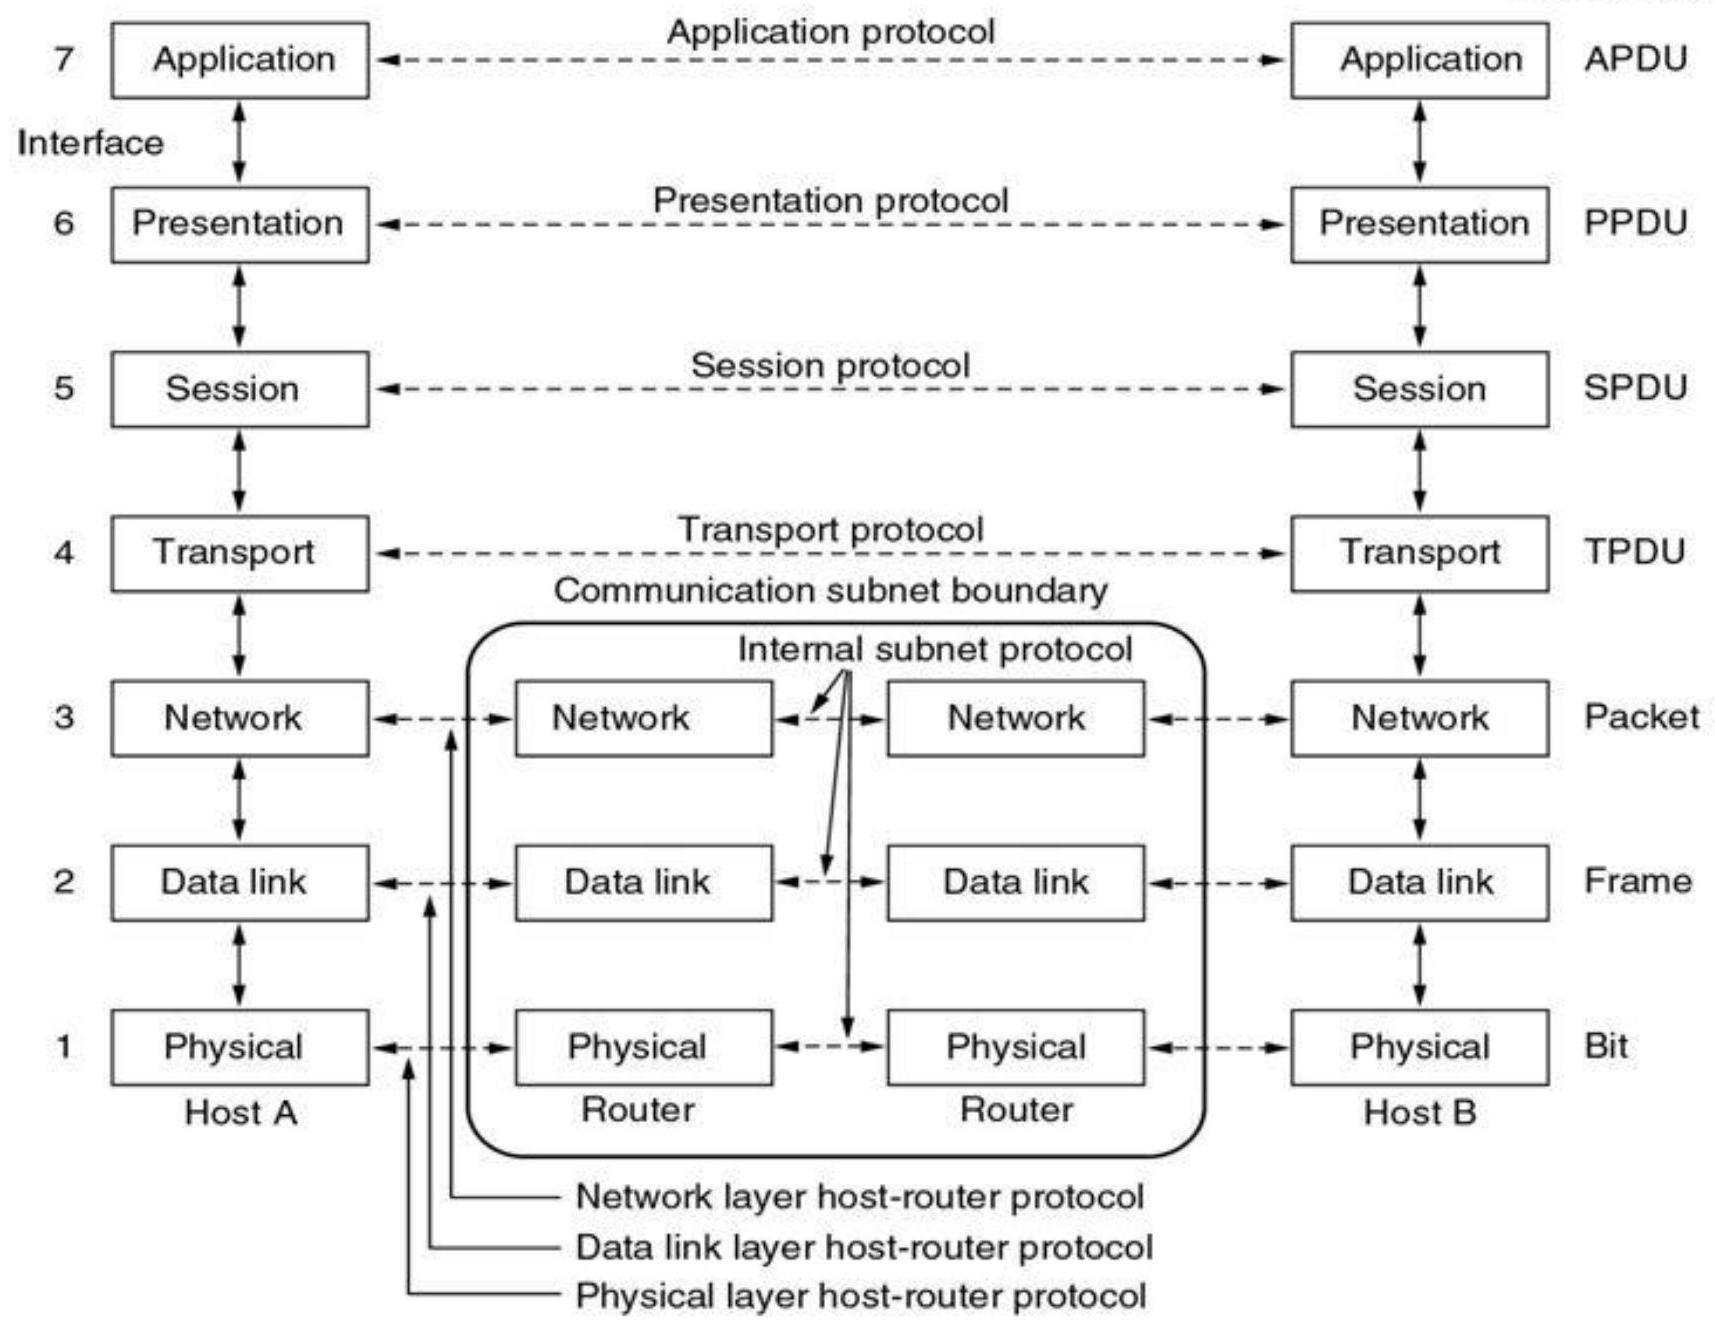
\includegraphics[max width=\textwidth]{2023_01_13_b07e3b4bcffdaab9792bg-010}
\end{center}


\os{newpage} item[{\rot\bf  Layer 7 }]~\\[-3ex]

\bi
  \ite Is the top layer in the system

  \ite establishes the connection between application programmes (e.g.: email, data transfer, etc.)

  \ite Basic services:

\ei
\bi
 \ite File exchange
 \ei


\bi
  \ite Management protocols for user access, file access rights, electronic mail, etc.
\ei


\os{newpage} item[{\rot\bf  Layer 6 }]~\\[-3ex]

\bi
  \ite It provides functions for protocol conversion, data transmission and data encryption

  \ite Takes over encoding \& decoding (e.g. EBCDIC in ASCII)

  \ite Takes over the definition of the formats and control characters for the exchange of the data

\ei


\os{newpage} item[{\rot\bf  Layer 6 }]~\\[-3ex]


\os{newpage} item[{\rot\bf  - Takes care of the syntax \& correctness of the data }]~\\[-3ex]

\os{newpage} item[{\rot\bf Layer 5 }]~\\[-3ex]

\os{newpage} item[{\rot\bf  - Controls the establishment, execution and termination of the connection }]~\\[-3ex]

\textbackslash author\{

\bi
  \ite Takes over monitoring of operating parameters, data \textbackslash  flow control, reconnection in case of error and \textbackslash  synchronisation between user actions
\}
\ei


\os{newpage} item[{\rot\bf  $\underline{\text { Layer } 4}$ }]~\\[-3ex]


\os{newpage} item[{\rot\bf  - Is the connection between application-oriented \& transport-oriented layers }]~\\[-3ex]

\bi
  \ite Ensures that all data packets reach the correct
recipient
\ei


\os{newpage} item[{\rot\bf  $\underline{\operatorname{Layer}} 4$ }]~\\[-3ex]

\bi
  \ite Establishing the data connection between two partners, data transport, flow control, error detection and correction

  \ite Ensuring completeness, uniqueness \& sequence of data blocks

  \ite Their services are divided into 4 classes

\ei


\os{newpage} item[{\rot\bf  $\underline{\operatorname{Layer} 4}$ }]~\\[-3ex]


\os{newpage} item[{\rot\bf  - Class O: }]~\\[-3ex]


\os{newpage} item[{\rot\bf  o Is the simplest }]~\\[-3ex]
\bi
 \ite No error handling
 \ei

\bi
 \ite there is no error control compared to layer 3
 \ei

\bi
 \ite One transport connection corresponds to exactly one network connection
 \ei



\os{newpage} item[{\rot\bf  Layer 4 }]~\\[-3ex]


\os{newpage} item[{\rot\bf  - Class 1: }]~\\[-3ex]
\bi
 \ite No error handling
 \ei

\bi
 \ite Attempts to correct errors reported by layer 3 and does not forward them to layer 5 .
 \ei

\bi
 \ite For example, if the transport connection is interrupted, an attempt can be made to rebuild it without this being noticed above layer 4 .
 \ei



\os{newpage} item[{\rot\bf  Layer 4 }]~\\[-3ex]


\os{newpage} item[{\rot\bf  - Class 2: }]~\\[-3ex]


\os{newpage} item[{\rot\bf  o can establish several transport connections (multiplex connection) }]~\\[-3ex]


\os{newpage} item[{\rot\bf  o In this case, the network connection may only be disconnected when the last transport connection has been terminated. }]~\\[-3ex]


\os{newpage} item[{\rot\bf  $\underline{\operatorname{Layer} 4}$ }]~\\[-3ex]


\os{newpage} item[{\rot\bf  - Class 3 : }]~\\[-3ex]


\os{newpage} item[{\rot\bf  o Covers the services of classes 1 \& 2 (error handling \& multiplex connections) }]~\\[-3ex]


\os{newpage} item[{\rot\bf  Layer 4 }]~\\[-3ex]

\bi
  \ite Class 4:
\ei
\bi
 \ite Contains, in addition to the functions of class 3, additional mechanisms for error detection/handling
 \ei


\bi
  \ite Especially in datagram-oriented networks (LAN), a connection-oriented service can be provided in this way (ensuring completeness, uniqueness and sequence of data blocks).
\ei


\os{newpage} item[{\rot\bf  Layer 4 }]~\\[-3ex]

\bi
  \ite Devices:
\ei
\bi
 \ite Gateway
 \ei



\os{newpage} item[{\rot\bf  Layer 3 }]~\\[-3ex]

\bi
  \ite is mainly used for data packet
transmission

  \ite Responsible for the choice of data
paths (routing)

  \ite for multiplexing several connections over individual sections

\ei


\os{newpage} item[{\rot\bf  Layer 3 }]~\\[-3ex]

\bi
  \ite For error handling, flow control \& flow control between the endpoints of a connection (not between the user processes).

  \ite Removal of bottlenecks (consequence of data
collisions)

\ei


\os{newpage} item[{\rot\bf  Layer 3 }]~\\[-3ex]

\bi
  \ite Devices:
\ei
\bi
 \ite Router
 \ei

\bi
 \ite Layer 3 Switch
 \ei



\os{newpage} item[{\rot\bf  Layer 2 }]~\\[-3ex]

\bi
  \ite Ensuring a functioning connection between two directly adjacent stations

  \ite Provides a defined framework for data transport, error detection and synchronisation of data

\ei


\os{newpage} item[{\rot\bf  Layer 2 }]~\\[-3ex]

\bi
  \ite Information is divided into blocks of appropriate length called frames and provided with check info for error detection/correction.

  \ite Flow control for the binary data

  \ite Transmitter \& receiver hardware addresses are added to the data frame

\ei


\os{newpage} item[{\rot\bf  Layer 2 }]~\\[-3ex]

\bi
  \ite For local networks, this layer is subdivided again: - 2 a (Media Access Control, MAC): Controls access to the transmission medium
\ei
\bi
 \ite 2 b (Logical Link Control, LLC): Layer 2 functions dependent on the transmission medium
 \ei



\os{newpage} item[{\rot\bf  Layer 2 }]~\\[-3ex]

\bi
  \ite Devices:
\ei
\bi
 \ite Bridge
 \ei


Switch


\os{newpage} item[{\rot\bf  Layer 1 }]~\\[-3ex]

\bi
  \ite Is the bottom layer

  \ite This is where the physical data transmission takes place

  \ite It defines the electrical, mechanical \& functional parameters for the physical connection of two units (e.g. level, modulation, cable, connector, transmission rate, etc.).

\ei


\os{newpage} item[{\rot\bf  Layer 1 }]~\\[-3ex]

\bi
  \ite Devices and network components:
\ei
\bi
 \ite Antenna
 \ei

\bi
 \ite Amplifier
 \ei

\bi
 \ite Plug and socket for the mains cable
 \ei

\bi
 \ite Repeater
 \ei

\bi
 \ite $\mathrm{Hub}$
 \ei

\bi
 \ite Transceiver
 \ei

\bi
 \ite T-piece and the end resistor
 \ei



\os{newpage} item[{\rot\bf  Communication between the layers }]~\\[-3ex]

Layer 7

Layer 6

\begin{center}
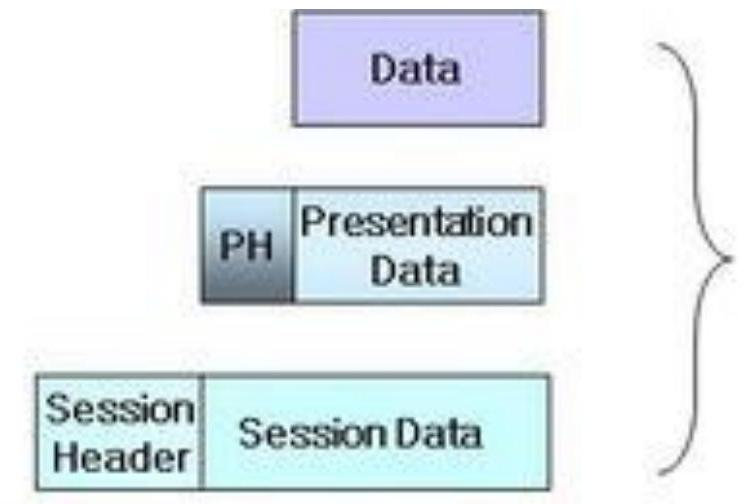
\includegraphics[max width=\textwidth]{2023_01_13_b07e3b4bcffdaab9792bg-032}
\end{center}

Layer 5

Layer 4

\begin{center}
\begin{tabular}{|c|c|}
\hline
TCP Header & TCP Data \\
\hline
MAC Header & IP Data \\
\hline
Ethernet/ Token-Ring Frame / X.25 / FR / ATM Data &  \\
\hline
\end{tabular}
\end{center}

Layer 3

Layer 1

Layer 2 TCP Frame

Application

Frame

IP Frame

MAC Frame


\os{newpage} item[{\rot\bf  Communication between the layers }]~\\[-3ex]

\begin{center}
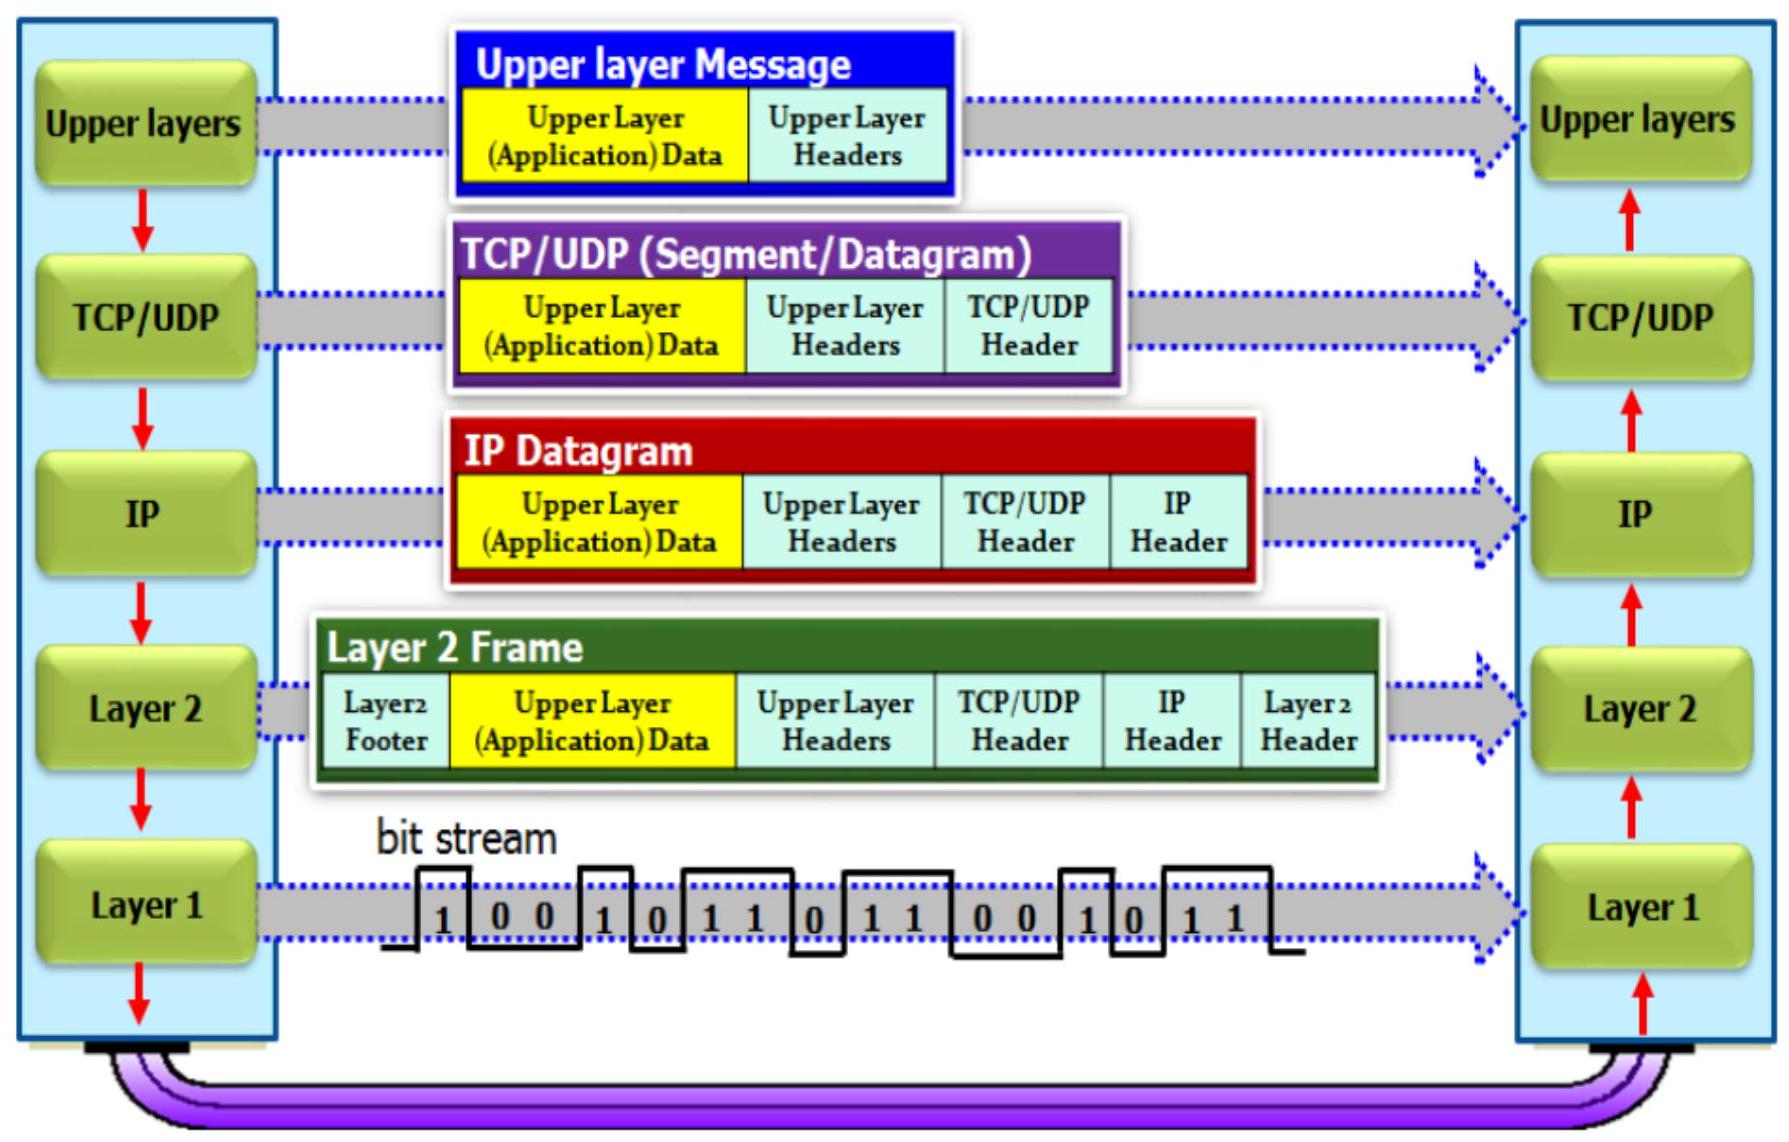
\includegraphics[max width=\textwidth]{2023_01_13_b07e3b4bcffdaab9792bg-033}
\end{center}

Figure 2. Encapsulation and Decapsulation of TCP/IP Protocol


\os{newpage} item[{\rot\bf  Devices }]~\\[-3ex]

OSI (Open Source Interconnection) 7 Layer Model

\begin{center}
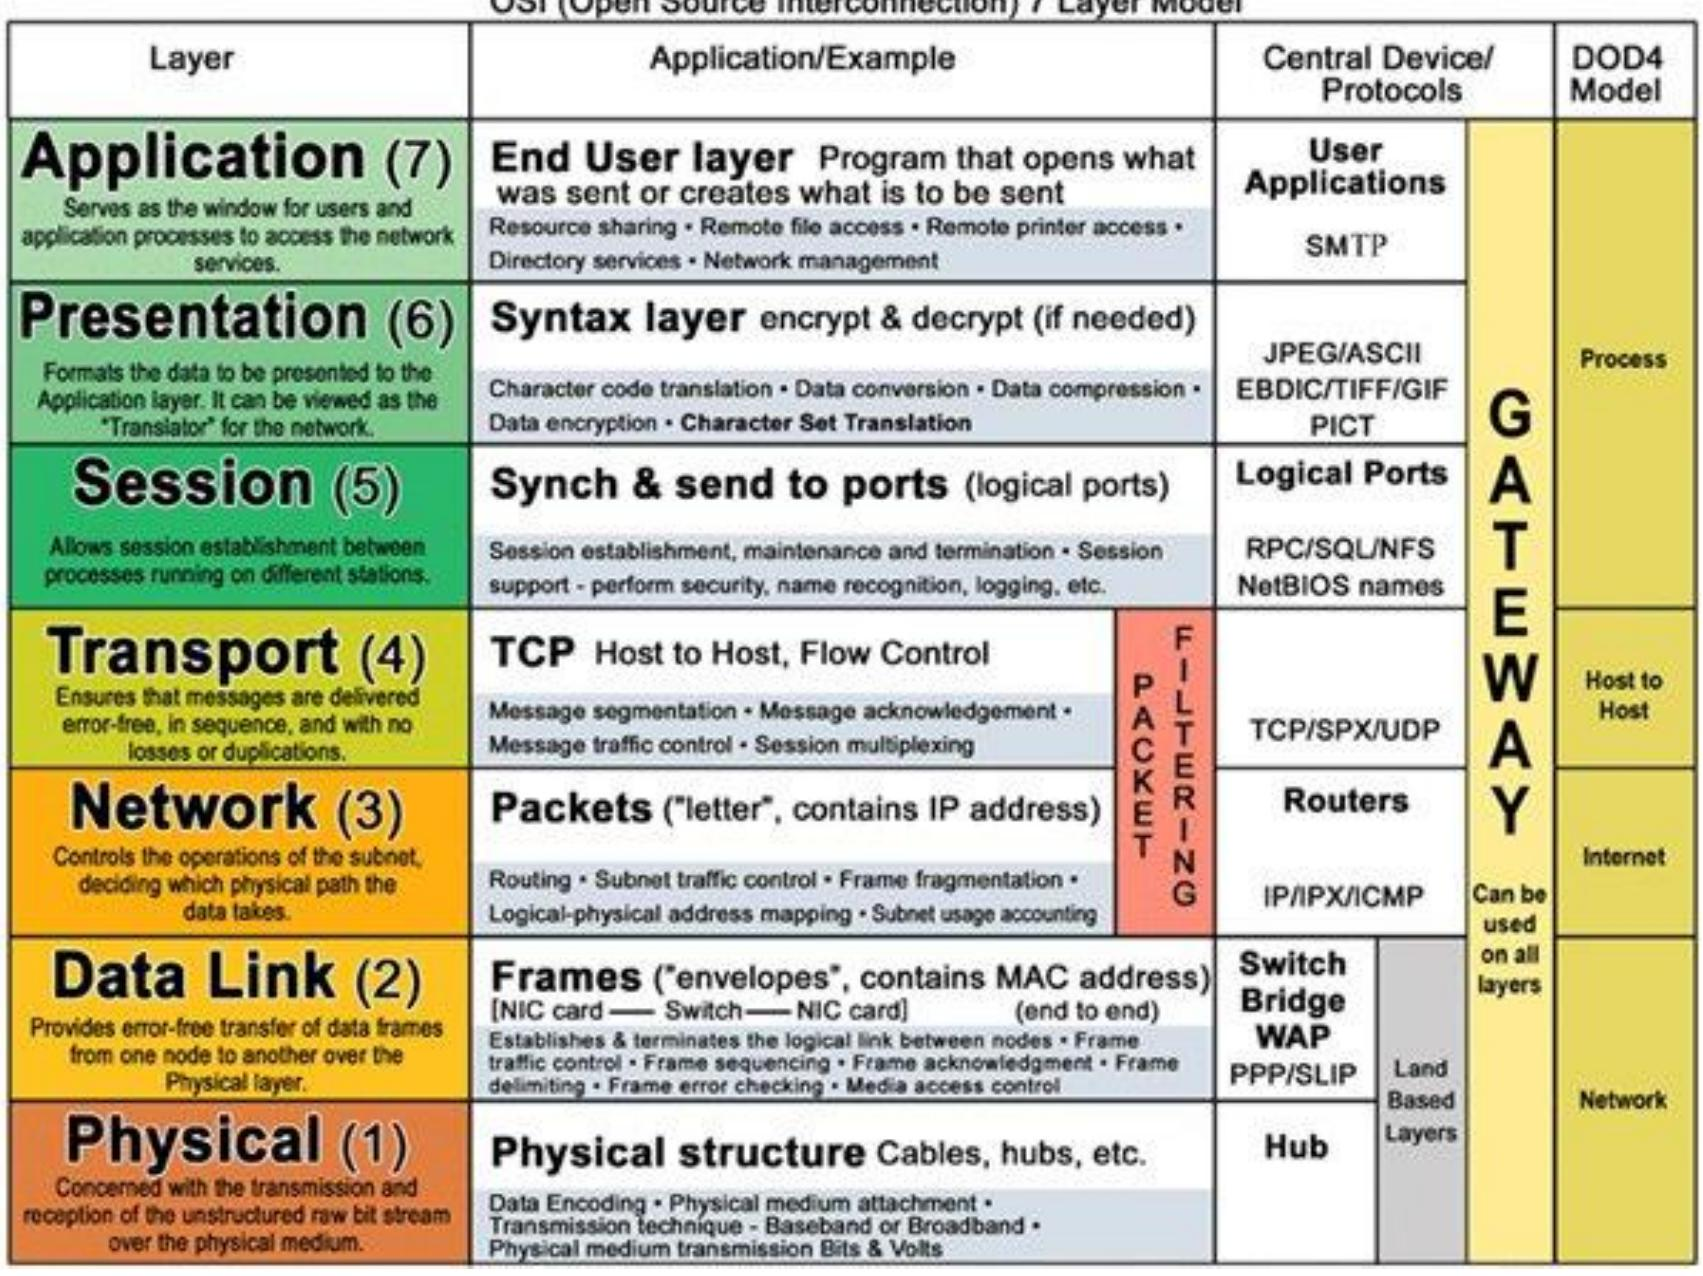
\includegraphics[max width=\textwidth]{2023_01_13_b07e3b4bcffdaab9792bg-034}
\end{center}


\os{newpage} item[{\rot\bf  Sources }]~\\[-3ex]

\bi
  \ite \href{http://www.wikipedia.de}{www.wikipedia.de} 17.12.05

  \ite \href{http://homepages.luc.edu/}{http://homepages.luc.edu/} bmontes/CIEP489Images/OSI-Model.gif 17.12.05

  \ite \href{http://www.netzmafia.de/skripten/netze/netzo.htm}{http://www.netzmafia.de/skripten/netze/netzo.htm} l\#0.1 17.12.05

  \ite My DVT binder 2004/05

\ei


\os{newpage} item[{\rot\bf  Transceiver Block Diagram }]~\\[-3ex]


\os{newpage} item[{\rot\bf  Transmitter }]~\\[-3ex]

Signal

\begin{center}
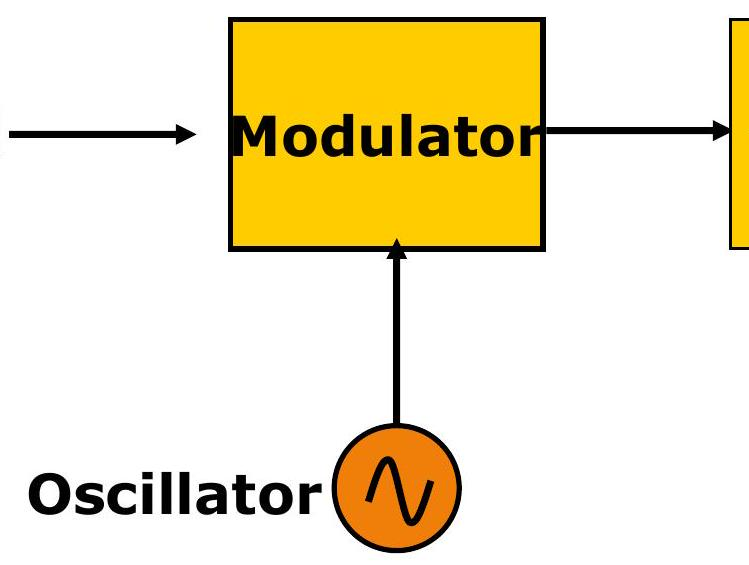
\includegraphics[max width=\textwidth]{2023_01_13_b07e3b4bcffdaab9792bg-037}
\end{center}

\begin{center}
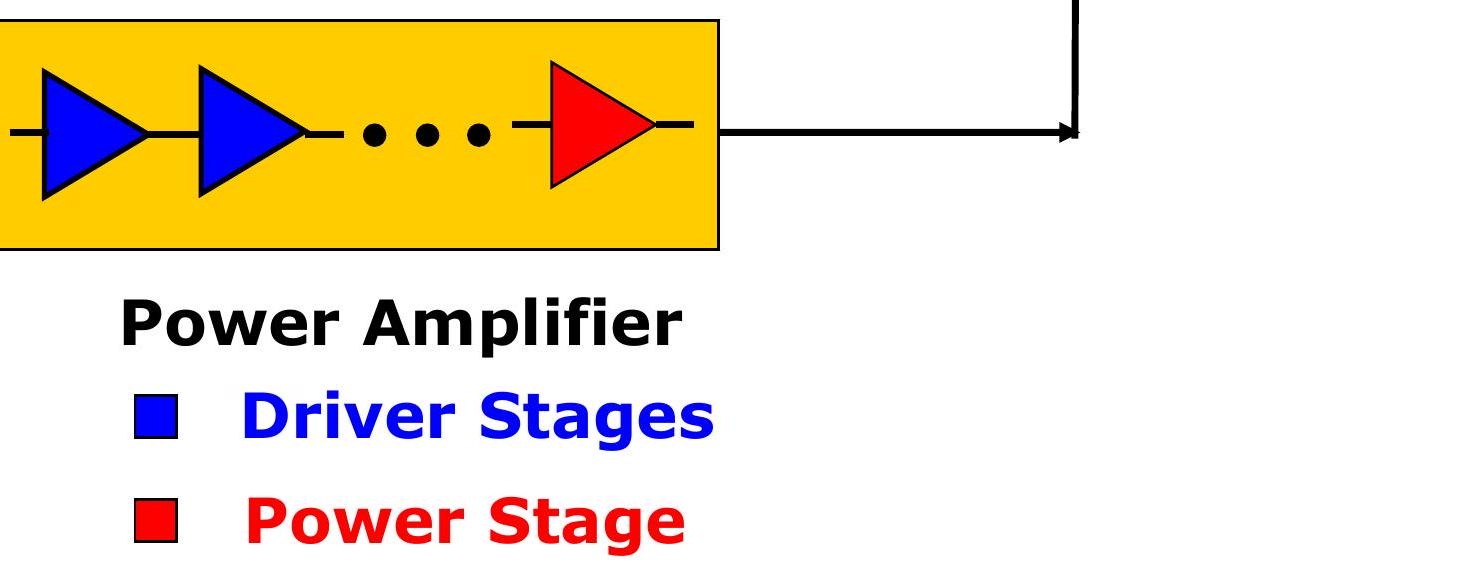
\includegraphics[max width=\textwidth]{2023_01_13_b07e3b4bcffdaab9792bg-037(1)}
\end{center}


\os{newpage} item[{\rot\bf  Receiver }]~\\[-3ex]

Antenna


\os{newpage} item[{\rot\bf  Low Noise Amplifier }]~\\[-3ex]

\begin{center}
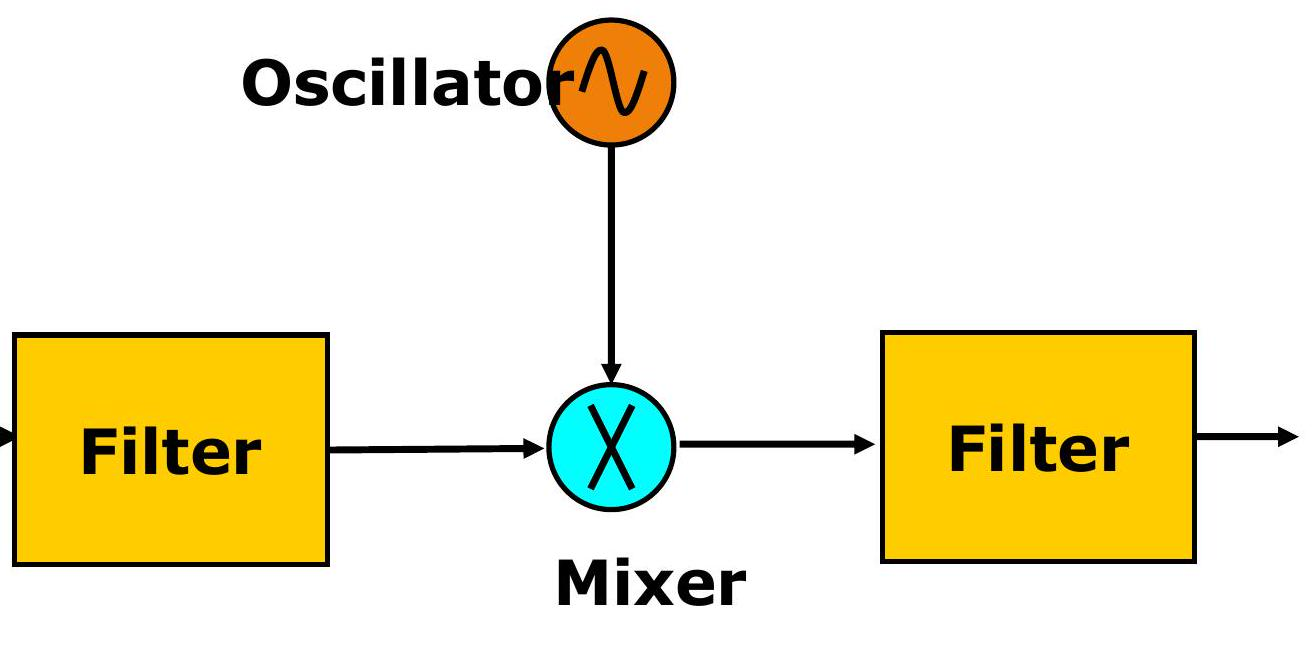
\includegraphics[max width=\textwidth]{2023_01_13_b07e3b4bcffdaab9792bg-038}
\end{center}

$\square$ Low Noise Amplifier

Gain-Stage Amplifier


\os{newpage} item[{\rot\bf  Transceiver $=$ Transmitter $+$ Receiver }]~\\[-3ex]

\begin{center}
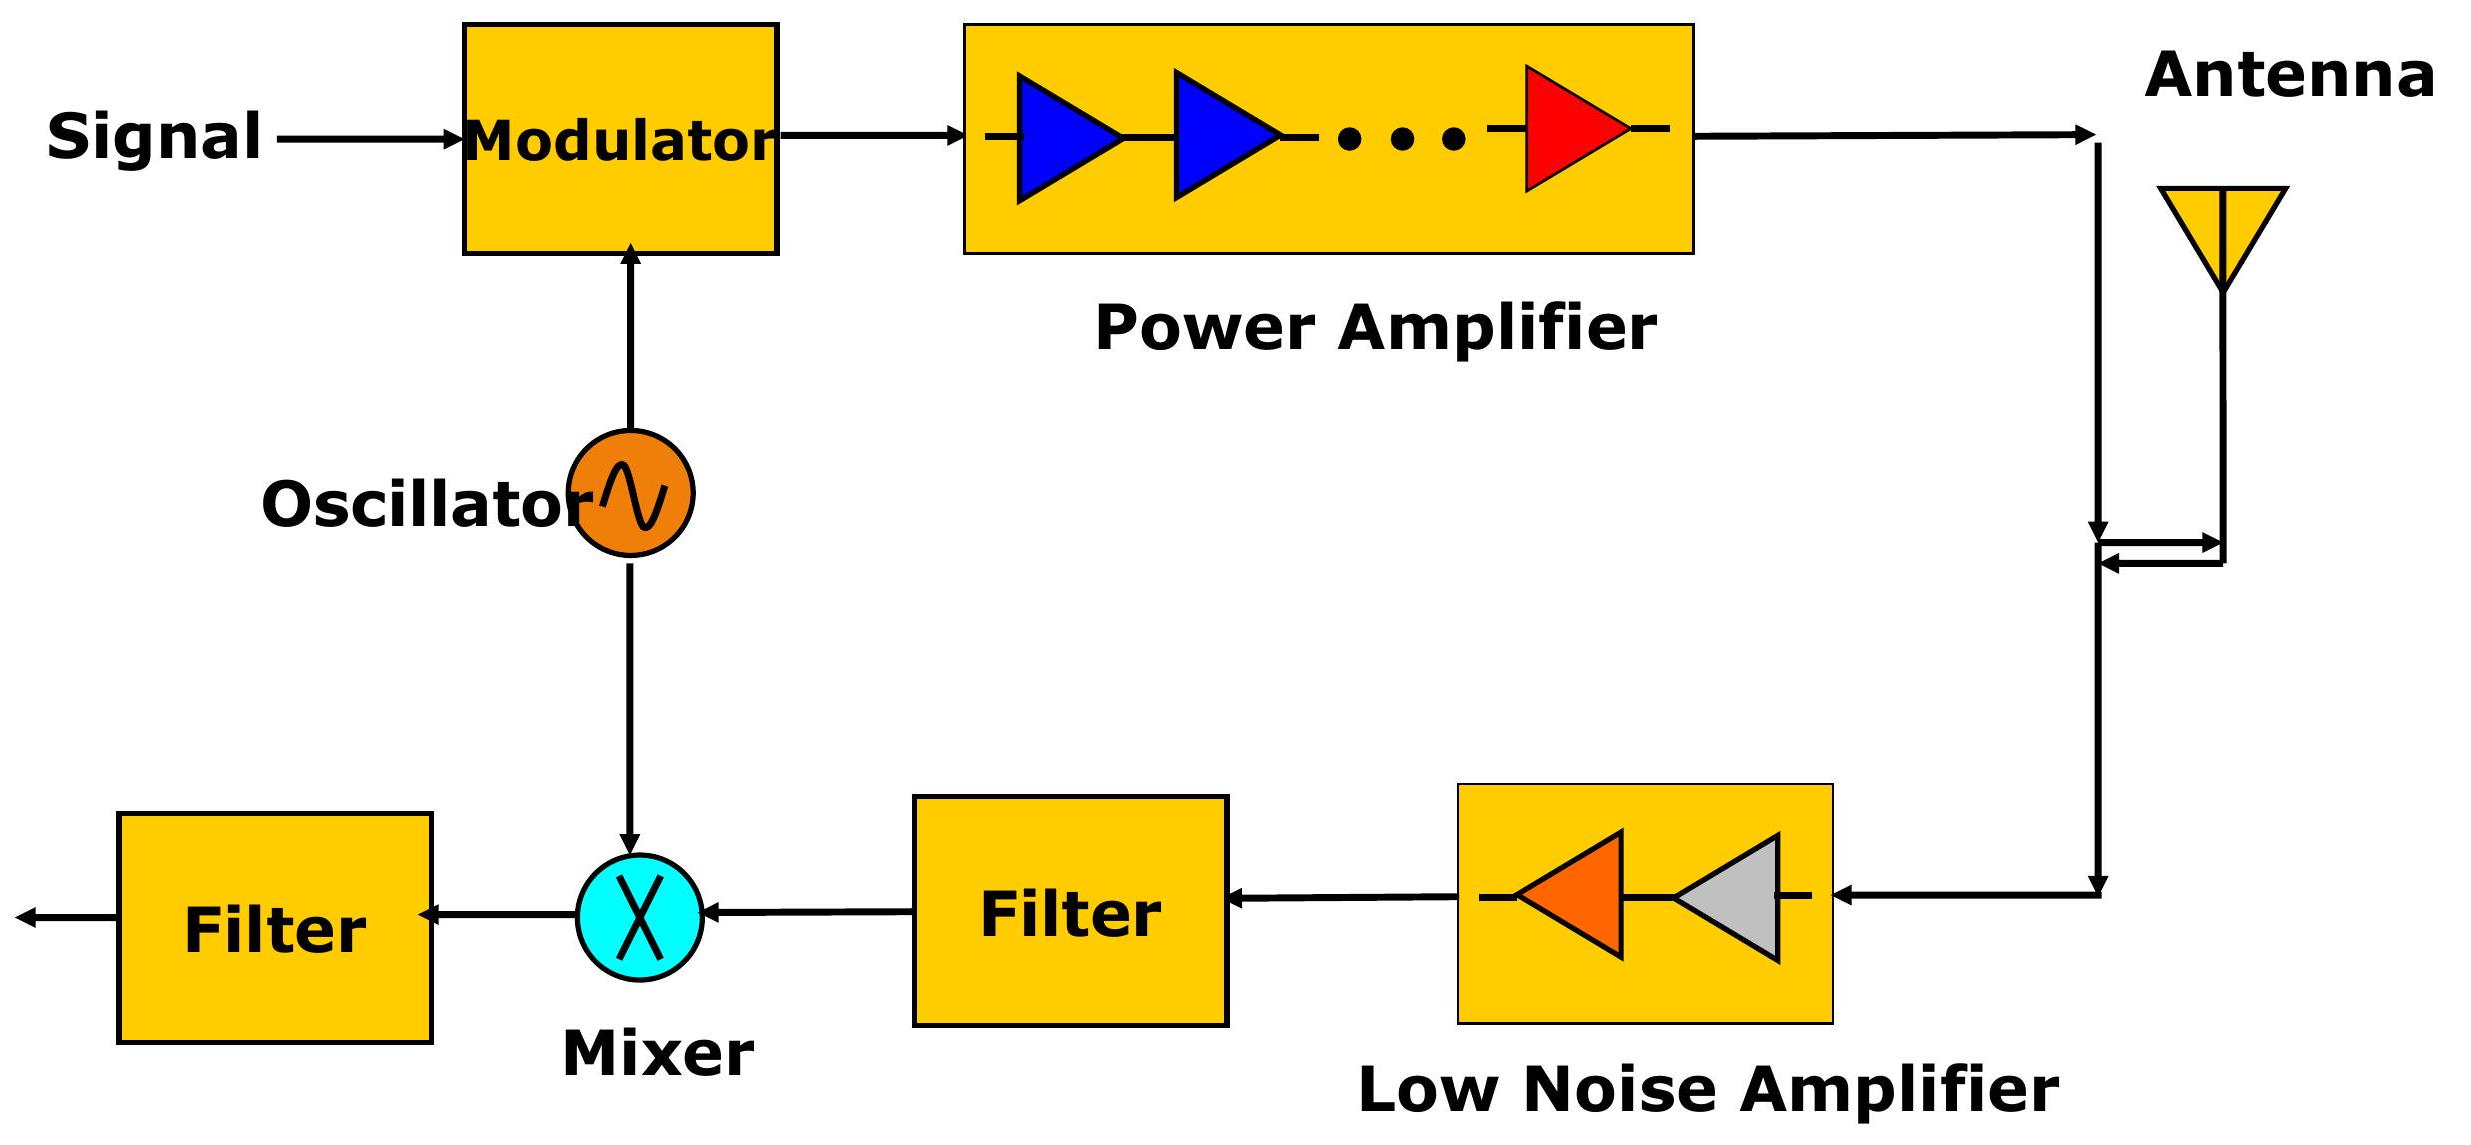
\includegraphics[max width=\textwidth]{2023_01_13_b07e3b4bcffdaab9792bg-039}
\end{center}


\os{newpage} item[{\rot\bf  Signal Encoding Techniques }]~\\[-3ex]


\os{newpage} item[{\rot\bf  Encoding Techniques }]~\\[-3ex]

\bi
  \ite Digital data, digital signal

  \ite Analog data, digital signal

  \ite Digital data, analog signal

  \ite Analog data, analog signal

\ei


\os{newpage} item[{\rot\bf  Digital Data, Digital Signal }]~\\[-3ex]

\bi
  \ite Digital signal

  \ite Discrete, discontinuous voltage pulses

\ei
\bi
 \ite Each pulse is a signal element
 \ei


\bi
  \ite Binary data encoded into signal elements
\ei


\os{newpage} item[{\rot\bf  Terms (1) }]~\\[-3ex]

\bi
  \ite Unipolar
\ei

All signal elements have same sign

\bi
  \ite Polar

  \ite One logic state represented by positive voltage the other by negative voltage

  \ite Data rate

\ei
\bi
 \ite Rate of data transmission in bits per second
 \ei


\bi
  \ite Duration or length of a bit
\ei
\bi
 \ite Time taken for transmitter to emit the bit
 \ei



\os{newpage} item[{\rot\bf  Terms (2) }]~\\[-3ex]

\bi
  \ite Modulation rate

  \ite Rate at which the signal level changes

  \ite Measured in baud = signal elements per second

  \ite Mark and Space

\ei
\bi
 \ite Binary 1 and Binary o respectively
 \ei



\os{newpage} item[{\rot\bf  Interpreting Signals }]~\\[-3ex]

\bi
  \ite Need to know
\ei
\bi
 \ite Timing of bits - when they start and end o Signal levels
 \ei


\bi
  \ite Factors affecting successful interpreting of signals o Signal to noise ratio
\ei
\bi
 \ite Data rate
 \ei

\bi
 \ite Bandwidth
 \ei



\os{newpage} item[{\rot\bf  Comparison of Encoding Schemes (1) }]~\\[-3ex]

\bi
  \ite Signal Spectrum

  \ite Lack of high frequencies reduces required bandwidth

  \ite Lack of dc component allows ac coupling via transformer, providing isolation

\ei
\bi
 \ite Concentrate power in the middle of the bandwidth
 \ei



\os{newpage} item[{\rot\bf  - Clocking }]~\\[-3ex]
\bi
 \ite Synchronizing transmitter and receiver
 \ei

\bi
 \ite External clock
 \ei

\bi
 \ite Sync mechanism based on signal
 \ei



\os{newpage} item[{\rot\bf  Comparison of Encoding Schemes (2) }]~\\[-3ex]

\bi
  \ite Error detection

  \ite Can be built in to signal encoding

  \ite Signal interference and noise immunity

\ei
\bi
 \ite Some codes are better than others
 \ei


\bi
  \ite Cost and complexity

  \ite Higher signal rate (\& thus data rate) lead to higher costs

\ei
\bi
 \ite Some codes require signal rate greater than data rate
 \ei



\os{newpage} item[{\rot\bf  Encoding Schemes }]~\\[-3ex]

\bi
  \ite Nonreturn to Zero-Level (NRZ-L)

  \ite Nonreturn to Zero Inverted (NRZI)

  \ite Bipolar -AMI

  \ite Pseudoternary

  \ite Manchester

  \ite Differential Manchester

  \ite B8ZS

  \ite $\mathrm{HDB}_{3}$

\ei


\os{newpage} item[{\rot\bf  Nonreturn to Zero-Level (NRZ-L) }]~\\[-3ex]

\bi
  \ite Two different voltages for 0 and 1 bits

  \ite Voltage constant during bit interval o no transition I.e. no return to zero voltage

  \ite e.g. Absence of voltage for zero, constant positive voltage for one

  \ite More often, negative voltage for one value and positive for the other

  \ite This is NRZ-L

\ei


\os{newpage} item[{\rot\bf  Nonreturn to Zero Inverted }]~\\[-3ex]

\bi
  \ite Nonreturn to zero inverted on ones

  \ite Constant voltage pulse for duration of bit

  \ite Data encoded as presence or absence of signal transition at beginning of bit time

  \ite Transition (low to high or high to low) denotes a binary 1

  \ite No transition denotes binary o

  \ite An example of differential encoding

\ei

\begin{center}
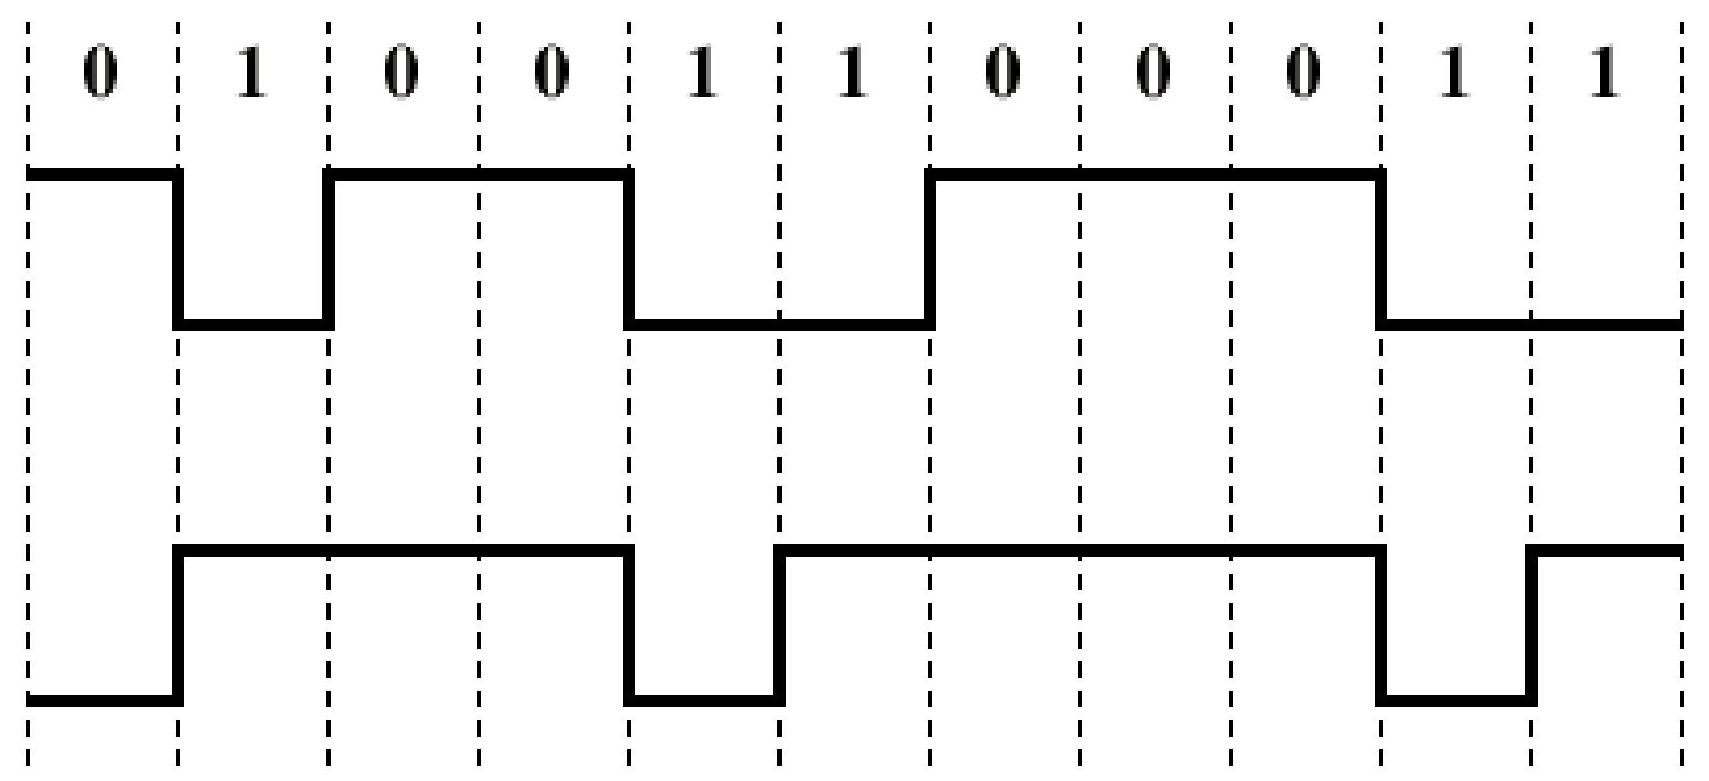
\includegraphics[max width=\textwidth]{2023_01_13_b07e3b4bcffdaab9792bg-051}
\end{center}


\os{newpage} item[{\rot\bf  Differential Encoding }]~\\[-3ex]

\bi
  \ite Data represented by changes rather than levels

  \ite More reliable detection of transition rather than level

  \ite In complex transmission layouts it is easy to lose sense of polarity

\ei


\os{newpage} item[{\rot\bf  NRZ pros and cons }]~\\[-3ex]

\bi
  \ite Pros
\ei
\bi
 \ite Easy to engineer
 \ei


\bi
  \ite Make good use of bandwidth

  \ite Cons

\ei
\bi
 \ite dc component
 \ei

\bi
 \ite Lack of synchronization capability
 \ei


\bi
  \ite Used for magnetic recording

  \ite Not often used for signal transmission

\ei


\os{newpage} item[{\rot\bf  Multilevel Binary }]~\\[-3ex]

\bi
  \ite Use more than two levels

  \ite Bipolar-AMI

\ei
\bi
 \ite zero represented by no line signal
 \ei

\bi
 \ite one represented by positive or negative pulse
 \ei

\bi
 \ite one pulses alternate in polarity
 \ei


\bi
  \ite No loss of sync if a long string of ones (zeros still a problem)
\ei
\bi
 \ite No net dc component
 \ei

\bi
 \ite Lower bandwidth
 \ei

\bi
 \ite Easy error detection
 \ei



\os{newpage} item[{\rot\bf  Pseudoternary }]~\\[-3ex]

\bi
  \ite One represented by absence of line signal

  \ite Zero represented by alternating positive and negative

  \ite No advantage or disadvantage over bipolar-AMI

\ei


\os{newpage} item[{\rot\bf  Bipolar-AMI and Pseudoternary }]~\\[-3ex]


\os{newpage} item[{\rot\bf  Bipolar-AMI }]~\\[-3ex]

(most recent preceding 1 bit has negative voltage)


\os{newpage} item[{\rot\bf  Pseudoternary }]~\\[-3ex]

(most recent preceding 0 bit has negative voltage)

\begin{center}
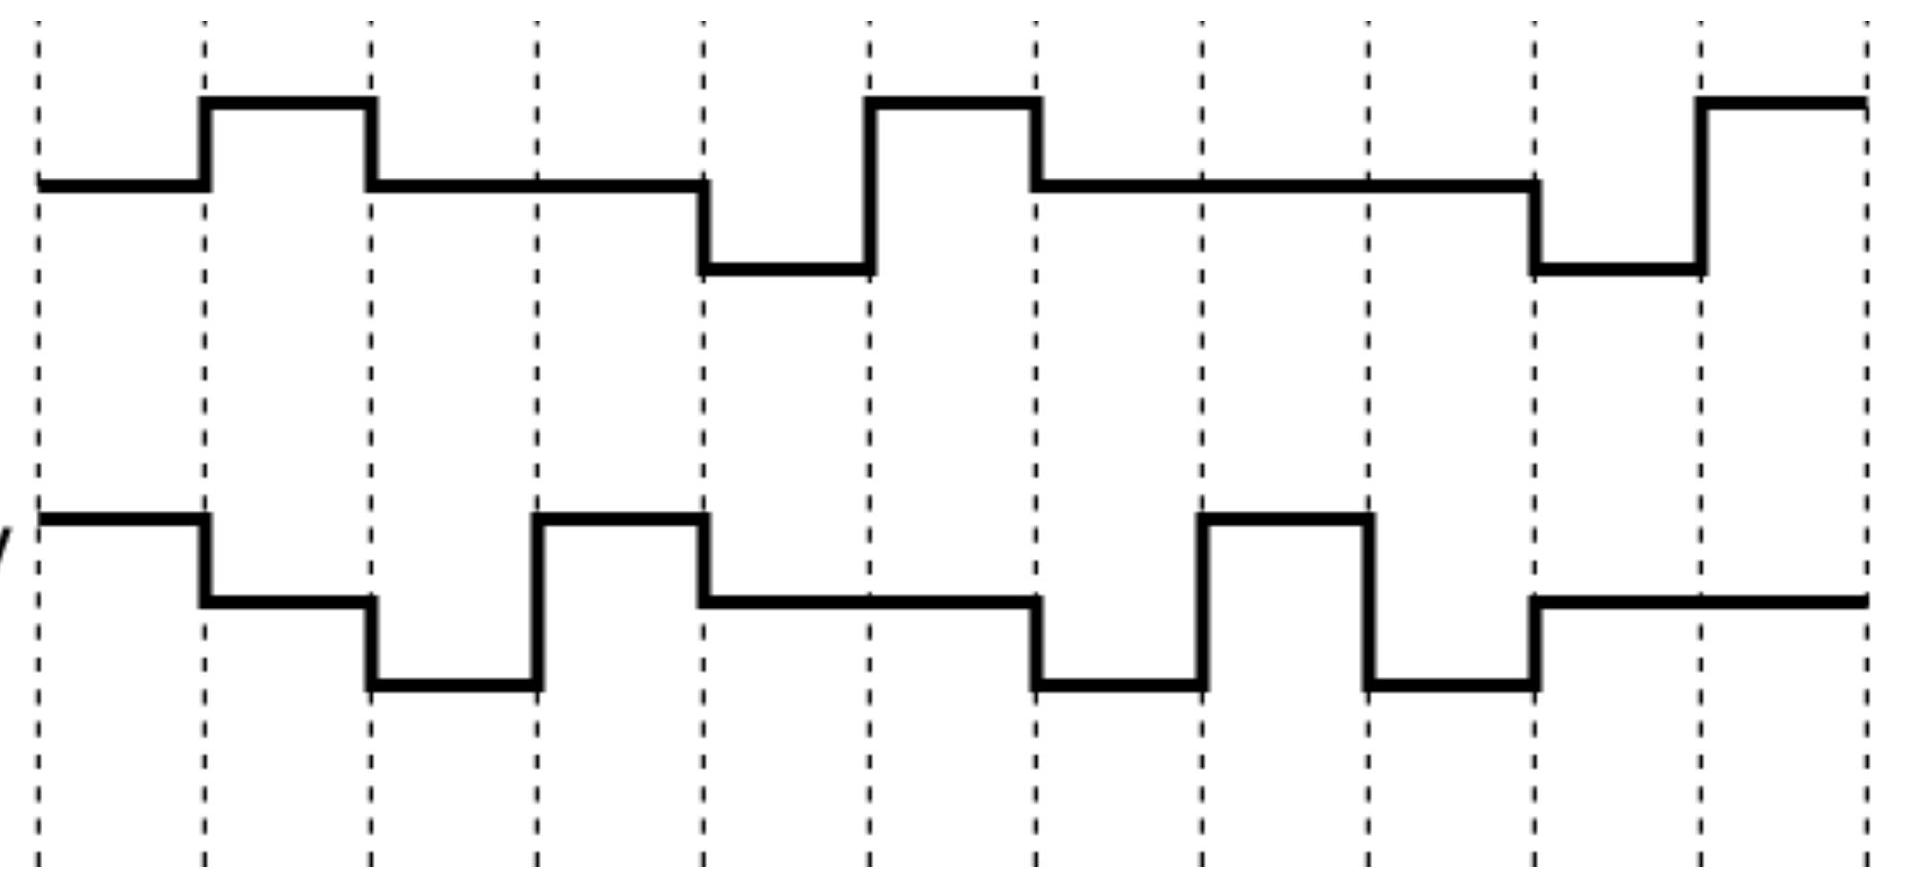
\includegraphics[max width=\textwidth]{2023_01_13_b07e3b4bcffdaab9792bg-056}
\end{center}


\os{newpage} item[{\rot\bf  Trade Off for Multilevel Binary }]~\\[-3ex]

\bi
  \ite Not as efficient as NRZ
\ei
\bi
 \ite Each signal element only represents one bit
 \ei

\bi
 \ite In a 3 level system could represent $\log _{2} 3=1.58$ bits
 \ei


\bi
  \ite Receiver must distinguish between three levels $(+\mathrm{A},-\mathrm{A}, \mathrm{o})$

  \ite Requires approx. $3 \mathrm{~dB}$ more signal power for same probability of bit error

\ei


\os{newpage} item[{\rot\bf  Biphase }]~\\[-3ex]

\bi
  \ite Manchester
\ei
\bi
 \ite Transition in middle of each bit period
 \ei

\bi
 \ite Transition serves as clock and data
 \ei

\bi
 \ite Low to high represents one
 \ei

\bi
 \ite High to low represents zero
 \ei

\bi
 \ite Used by IEEE 802.3
 \ei


\bi
  \ite Differential Manchester
\ei
\bi
 \ite Midbit transition is clocking only
 \ei

\bi
 \ite Transition at start of a bit period represents zero
 \ei

\bi
 \ite No transition at start of a bit period represents one
 \ei

\bi
 \ite Note: this is a differential encoding scheme
 \ei

\bi
 \ite Used by IEEE 802.5
 \ei



\os{newpage} item[{\rot\bf  Manchester Encoding }]~\\[-3ex]


\os{newpage} item[{\rot\bf  Manchester Encoding }]~\\[-3ex]

\begin{center}
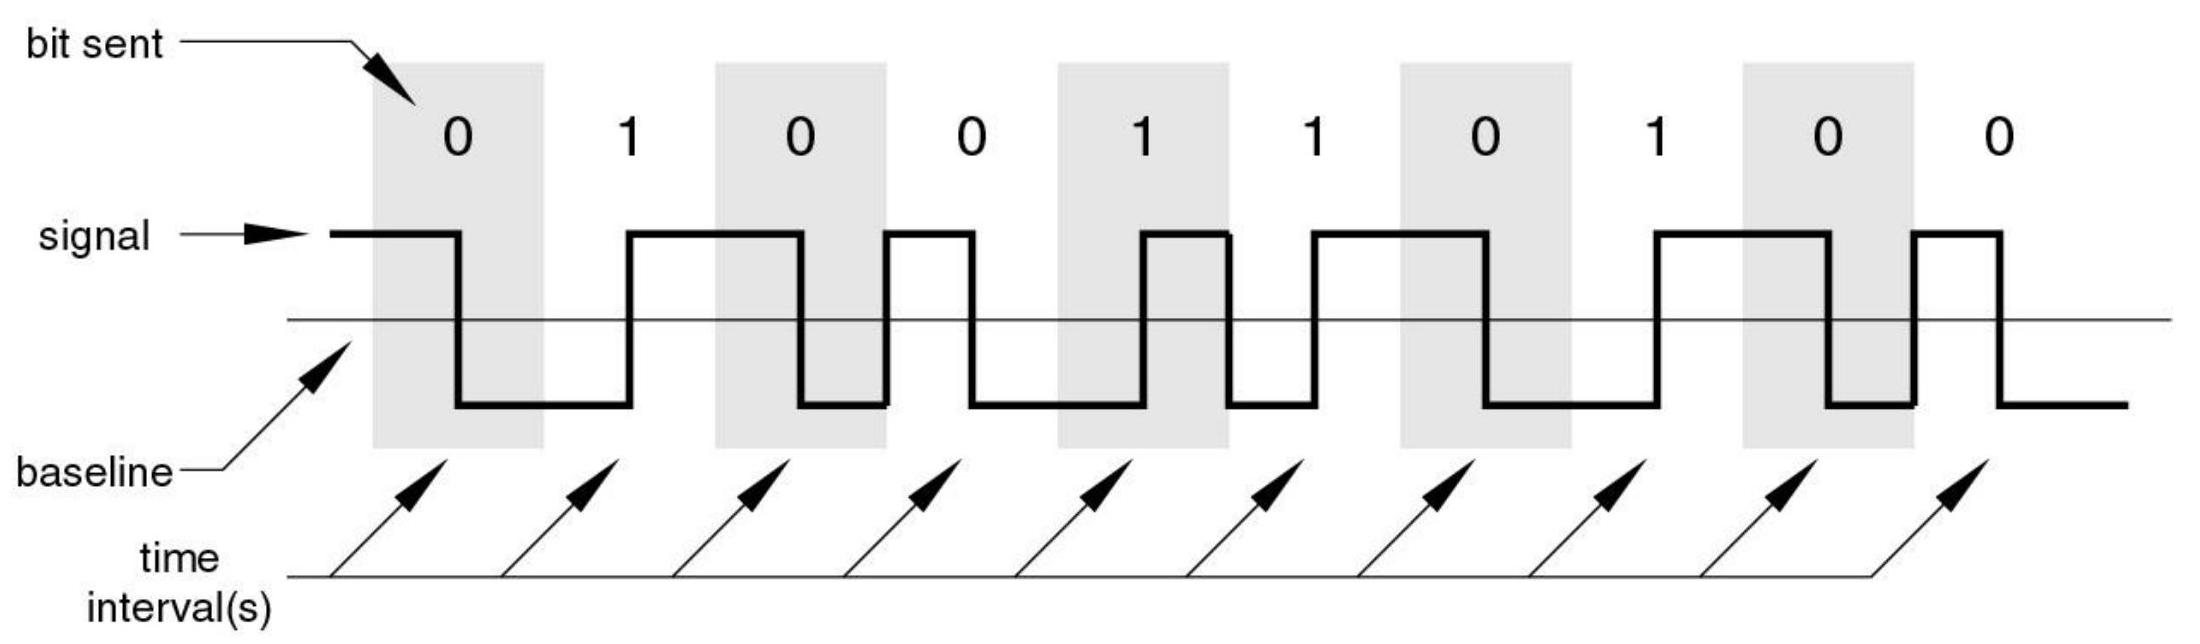
\includegraphics[max width=\textwidth]{2023_01_13_b07e3b4bcffdaab9792bg-059}
\end{center}


\os{newpage} item[{\rot\bf  Differential Manchester Encoding }]~\\[-3ex]


\os{newpage} item[{\rot\bf  Differential Manchester Encoding }]~\\[-3ex]

\begin{center}
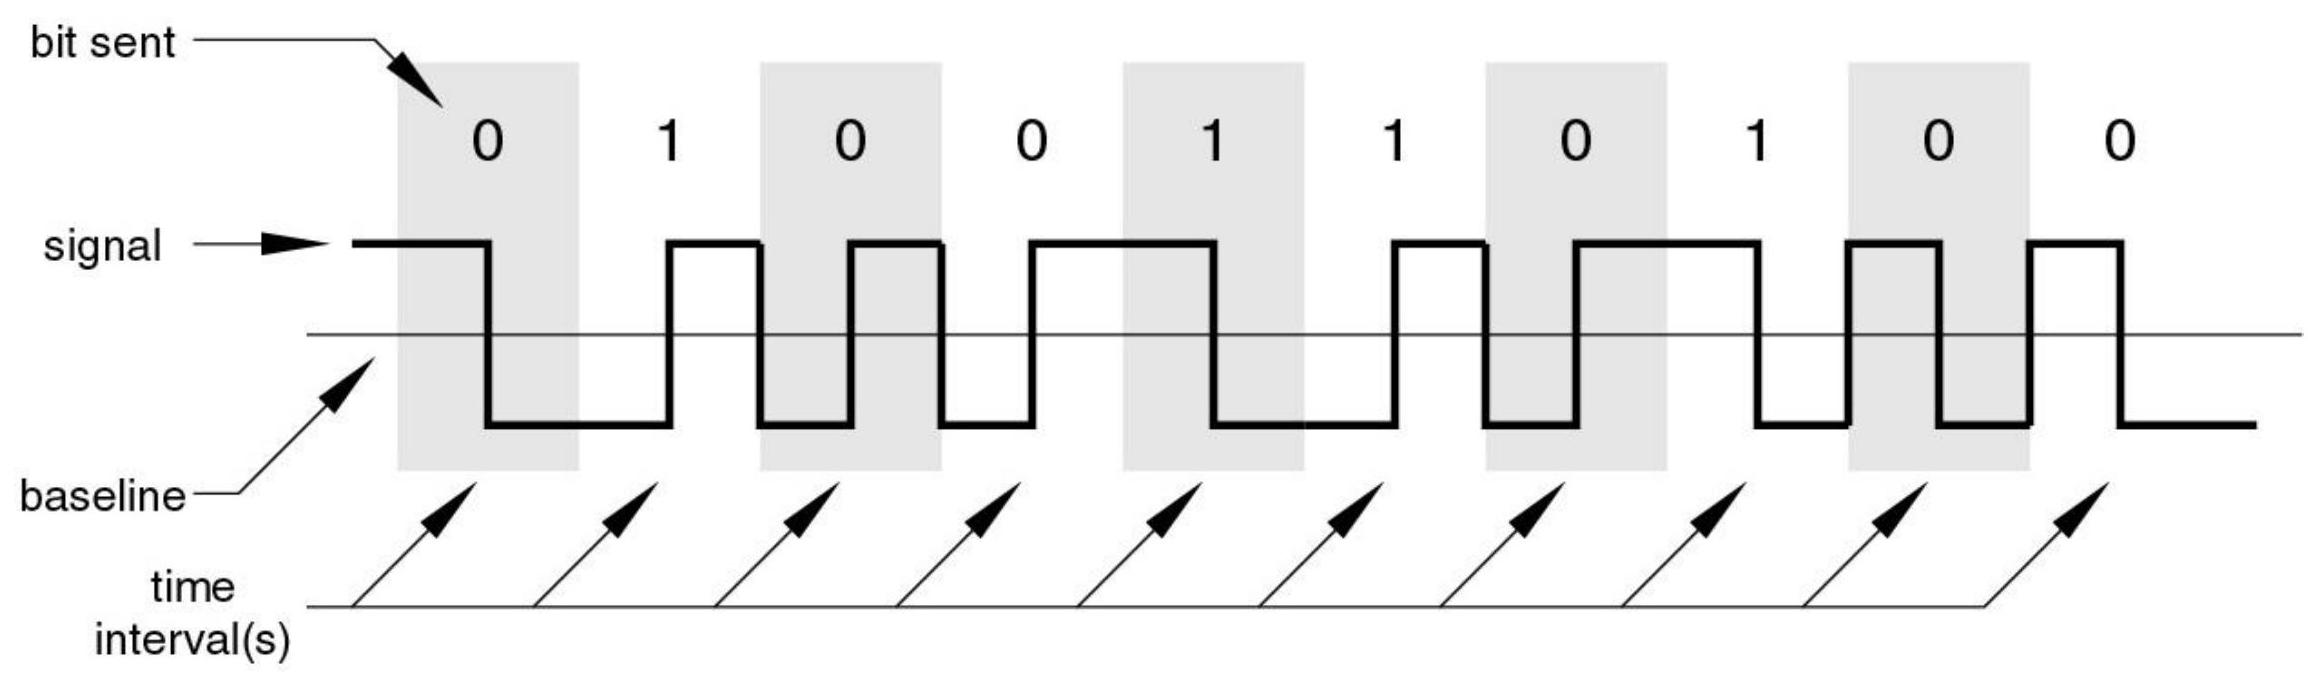
\includegraphics[max width=\textwidth]{2023_01_13_b07e3b4bcffdaab9792bg-060}
\end{center}

\os{newpage} item[{\rot\bf Biphase Pros and Cons }]~\\[-3ex]

\os{newpage} item[{\rot\bf  - Con }]~\\[-3ex]

At least one transition per bit time and possibly two
 - Maximum modulation rate is twice NRZ

 o Requires more bandwidth

\os{newpage} item[{\rot\bf  - Pros }]~\\[-3ex]




\os{newpage} item[{\rot\bf  Modulation Rate }]~\\[-3ex]

5 bits $=5 \mu \mathrm{sec}$

\begin{center}
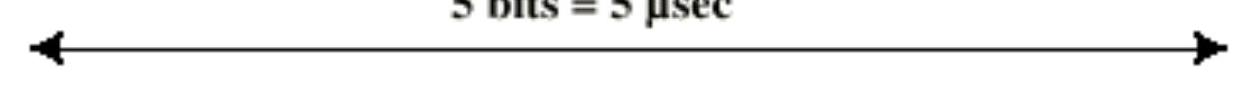
\includegraphics[max width=\textwidth]{2023_01_13_b07e3b4bcffdaab9792bg-062}
\end{center}

1

1

1

1

1

NRZI
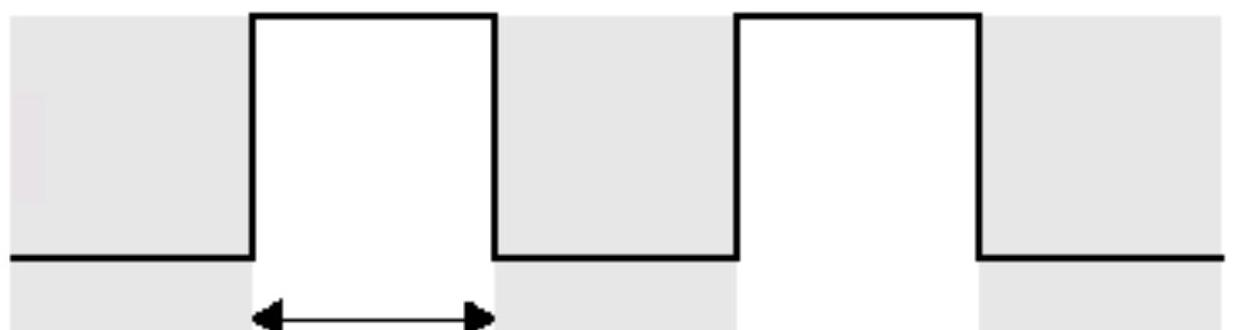
\includegraphics[max width=\textwidth, center]{2023_01_13_b07e3b4bcffdaab9792bg-062(1)}

Manchester

1 bit $=$

1 signal element $=$

1 μ $\mathrm{sec}$

\begin{center}
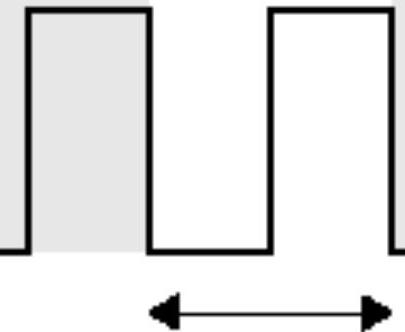
\includegraphics[max width=\textwidth]{2023_01_13_b07e3b4bcffdaab9792bg-062(2)}
\end{center}

$1 \mathrm{bit}=$

l $\mu$ sec

\begin{center}

\includegraphics[max width=\textwidth]{2023_01_13_b07e3b4bcffdaab9792bg-062(3)}
\end{center}

\begin{center}

\includegraphics[max width=\textwidth]{2023_01_13_b07e3b4bcffdaab9792bg-062(4)}
\end{center}

1

1 signal element $=$

$0.5 \mu \mathrm{sec}$


\os{newpage} item[{\rot\bf  Scrambling }]~\\[-3ex]

\bi
  \ite Use scrambling to replace sequences that would produce constant voltage

  \ite Filling sequence

  \ite Must produce enough transitions to sync

  \ite Must be recognized by receiver and replace with original

  \ite Same length as original

  \ite No dc component

  \ite No long sequences of zero level line signal

  \ite No reduction in data rate

  \ite Error detection capability

\ei


\os{newpage} item[{\rot\bf  B8ZS }]~\\[-3ex]

\bi
  \ite Bipolar With 8 Zeros Substitution

  \ite Based on bipolar-AMI

  \ite If octet of all zeros and last voltage pulse preceding was positive encode as $000+-0-+$

  \ite If octet of all zeros and last voltage pulse preceding was negative encode as 000-+0+-

  \ite Causes two violations of AMI code

  \ite Unlikely to occur as a result of noise

  \ite Receiver detects and interprets as octet of all zeros

\ei


\os{newpage} item[{\rot\bf  $\mathrm{HDB}_{3}$ }]~\\[-3ex]

\bi
  \ite High Density Bipolar 3 Zeros

  \ite Based on bipolar-AMI

  \ite String of four zeros replaced with one or two pulses

\ei


\os{newpage} item[{\rot\bf  B8ZS and $\mathrm{HDB}_{3}$ }]~\\[-3ex]

\begin{center}
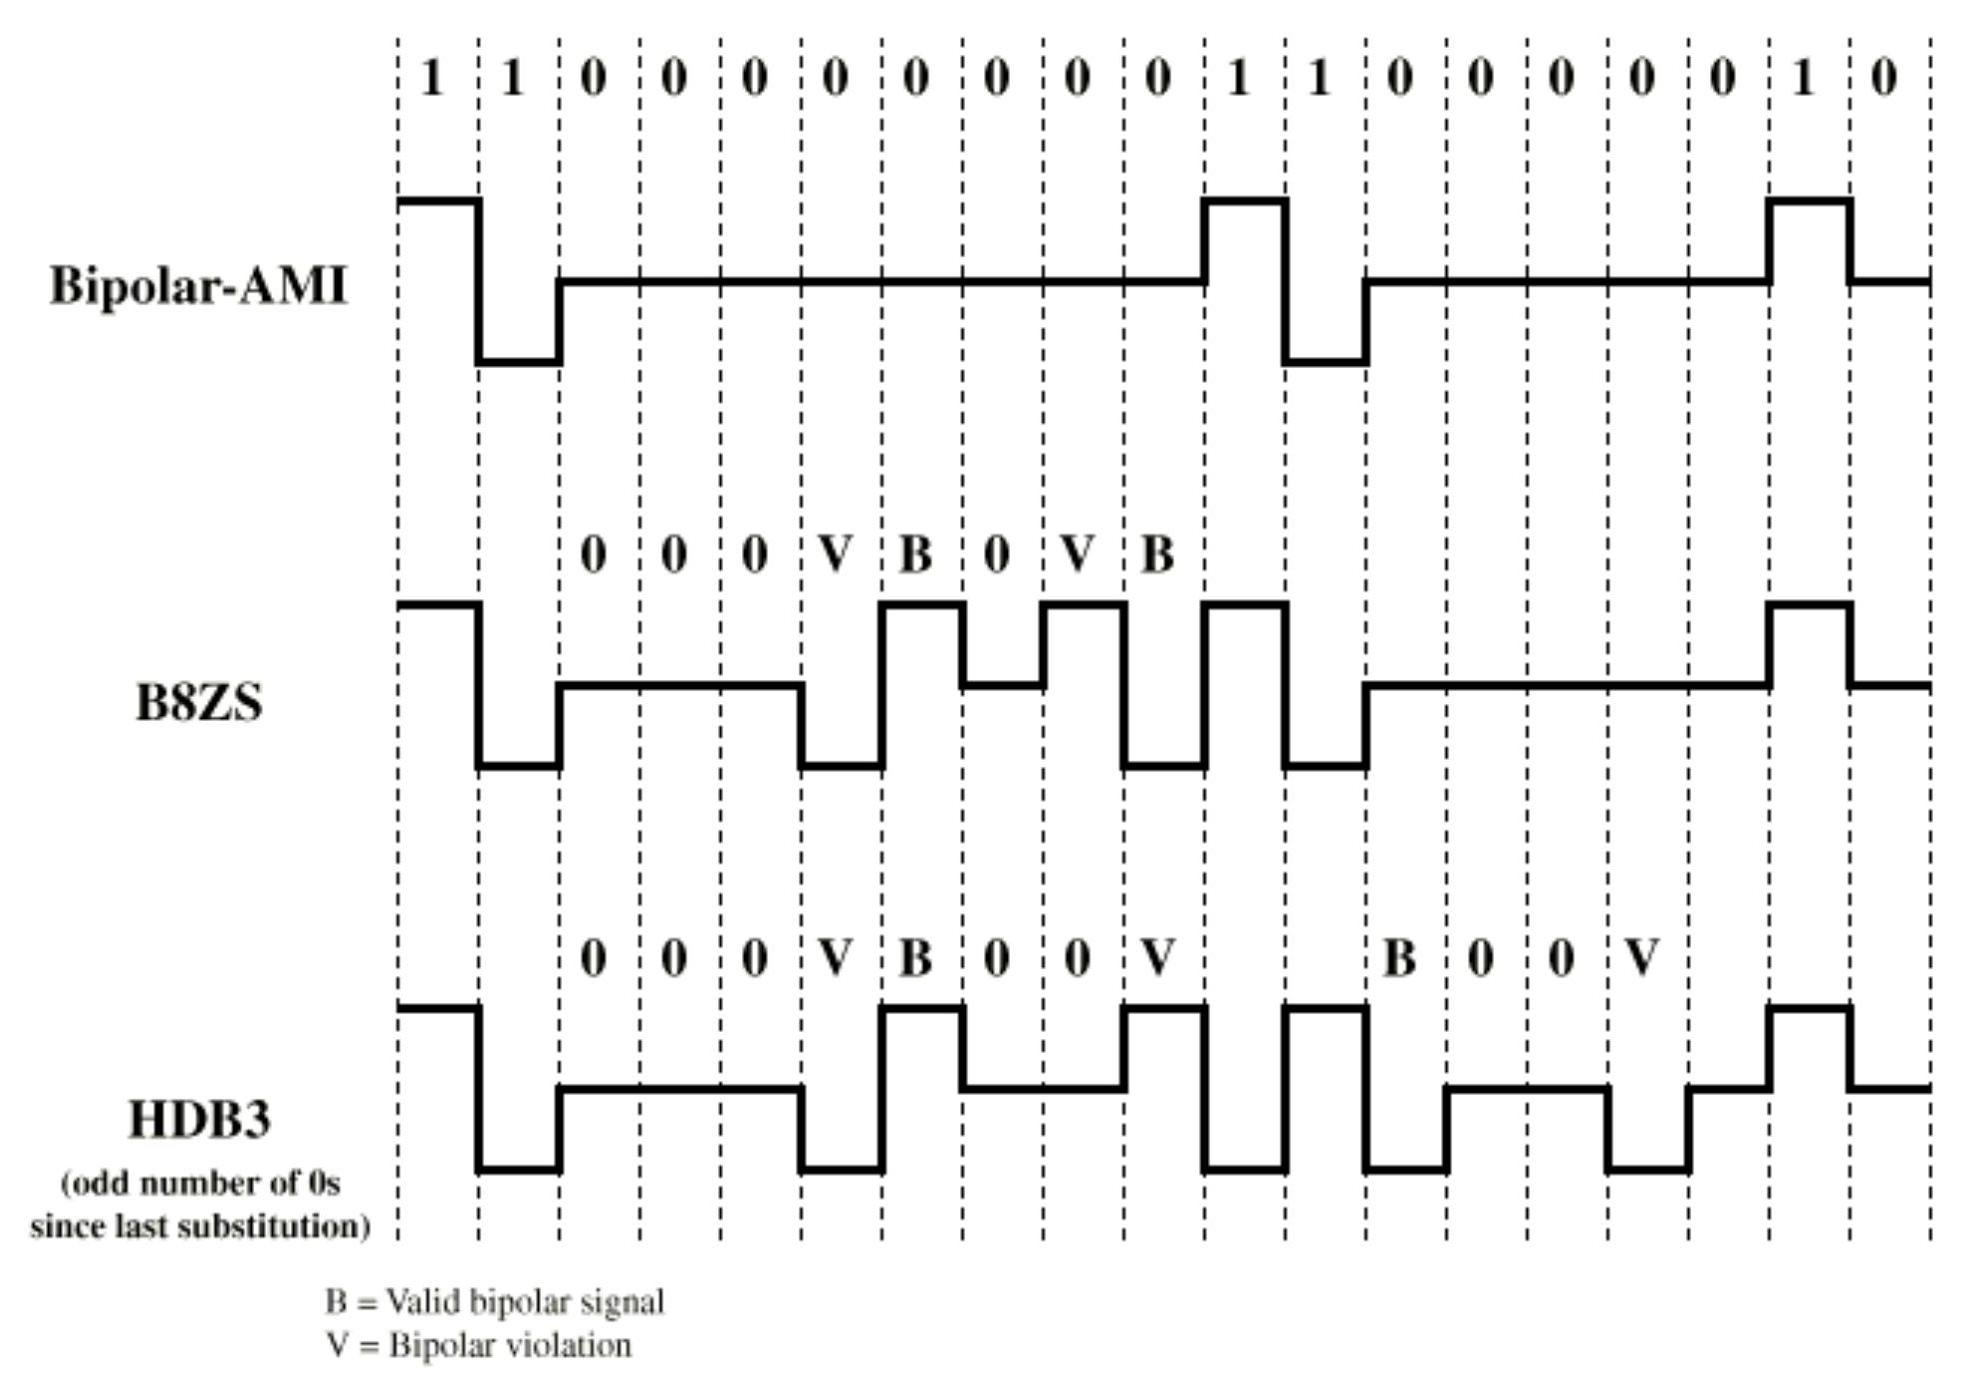
\includegraphics[max width=\textwidth]{2023_01_13_b07e3b4bcffdaab9792bg-066}
\end{center}


\os{newpage} item[{\rot\bf  Digital Data, Analog Signal }]~\\[-3ex]

\bi
  \ite Public telephone system o $300 \mathrm{~Hz}$ to $3400 \mathrm{~Hz}$
\ei
\bi
 \ite Use modem (modulator-demodulator)
 \ei


\bi
  \ite Amplitude shift keying (ASK)

  \ite Frequency shift keying (FSK)

  \ite Phase shift keying (PK)

\ei


\os{newpage} item[{\rot\bf  Modulation Techniques }]~\\[-3ex]

(a) ASK

\begin{center}
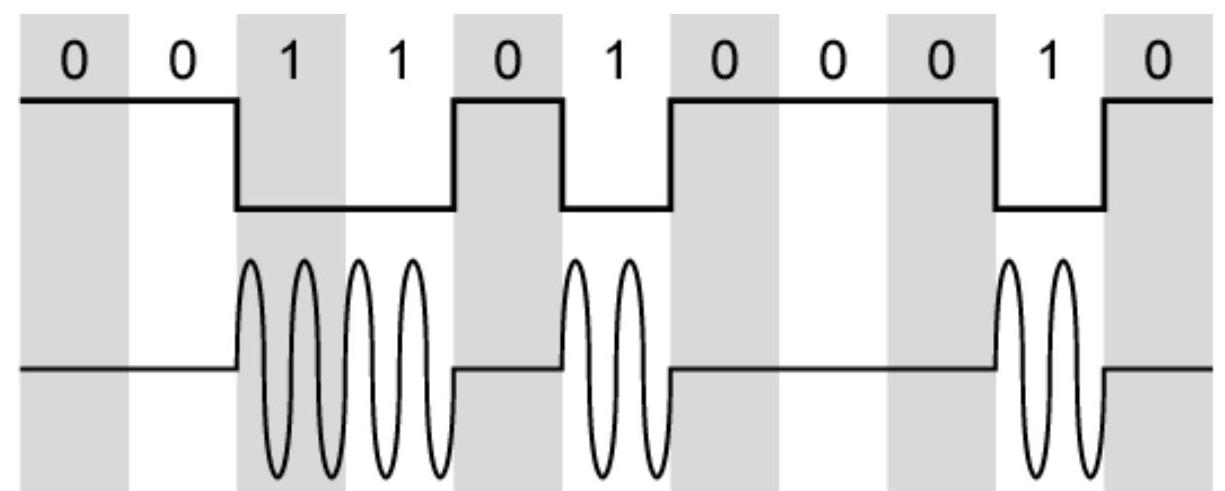
\includegraphics[max width=\textwidth]{2023_01_13_b07e3b4bcffdaab9792bg-068}
\end{center}

(b) BFSK

\begin{center}
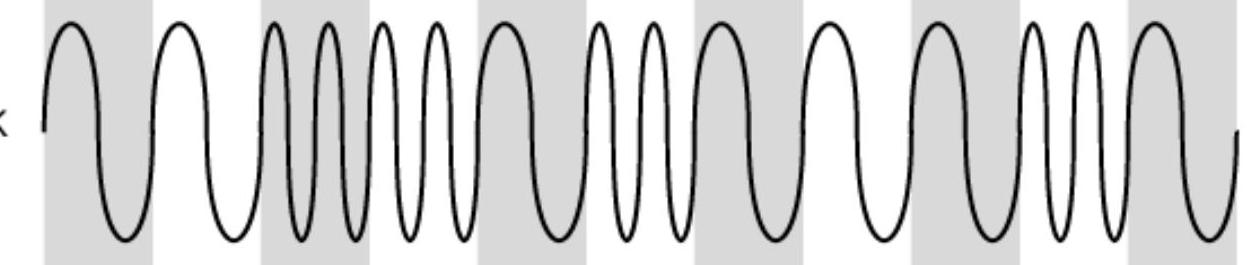
\includegraphics[max width=\textwidth]{2023_01_13_b07e3b4bcffdaab9792bg-068(1)}
\end{center}

(c) BPSK

\begin{center}
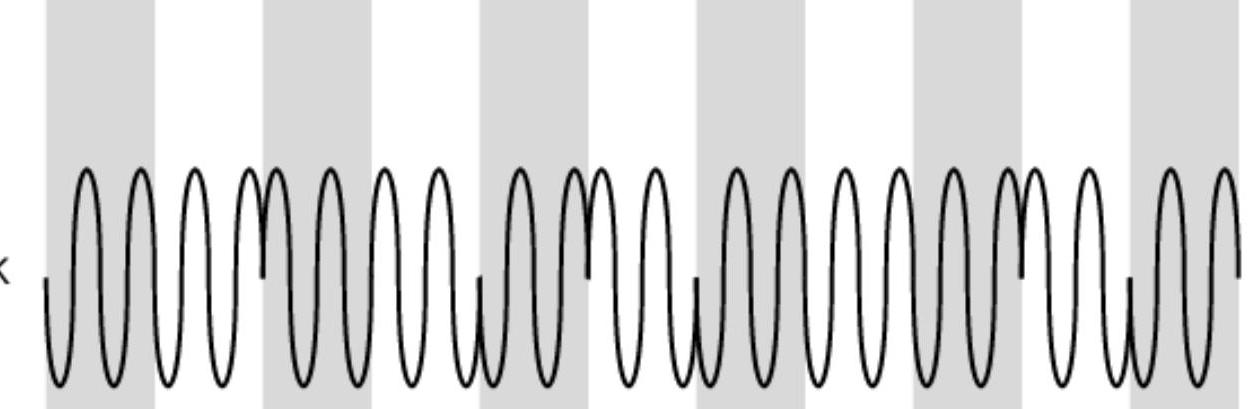
\includegraphics[max width=\textwidth]{2023_01_13_b07e3b4bcffdaab9792bg-068(2)}
\end{center}


\os{newpage} item[{\rot\bf  Amplitude Shift Keying }]~\\[-3ex]

\bi
  \ite Values represented by different amplitudes of carrier

  \ite Usually, one amplitude is zero

\ei
\bi
 \ite i.e. presence and absence of carrier is used
 \ei


\bi
  \ite Susceptible to sudden gain changes

  \ite Inefficient

  \ite Up to 120obps on voice grade lines

  \ite Used over optical fiber

\ei


\os{newpage} item[{\rot\bf  Binary Frequency Shift Keying }]~\\[-3ex]

\bi
  \ite Most common form is binary FSK (BFSK)

  \ite Two binary values represented by two different frequencies (near carrier)

  \ite Less susceptible to error than ASK

  \ite Up to 120obps on voice grade lines

  \ite High frequency radio

  \ite Even higher frequency on LANs using co-ax

\ei


\os{newpage} item[{\rot\bf  Multiple FSK }]~\\[-3ex]

\bi
  \ite More than two frequencies used

  \ite More bandwidth efficient

  \ite More prone to error

  \ite Each signalling element represents more than one bit

\ei


\os{newpage} item[{\rot\bf  FSK on Voice Grade Line }]~\\[-3ex]

signal strength

\begin{center}
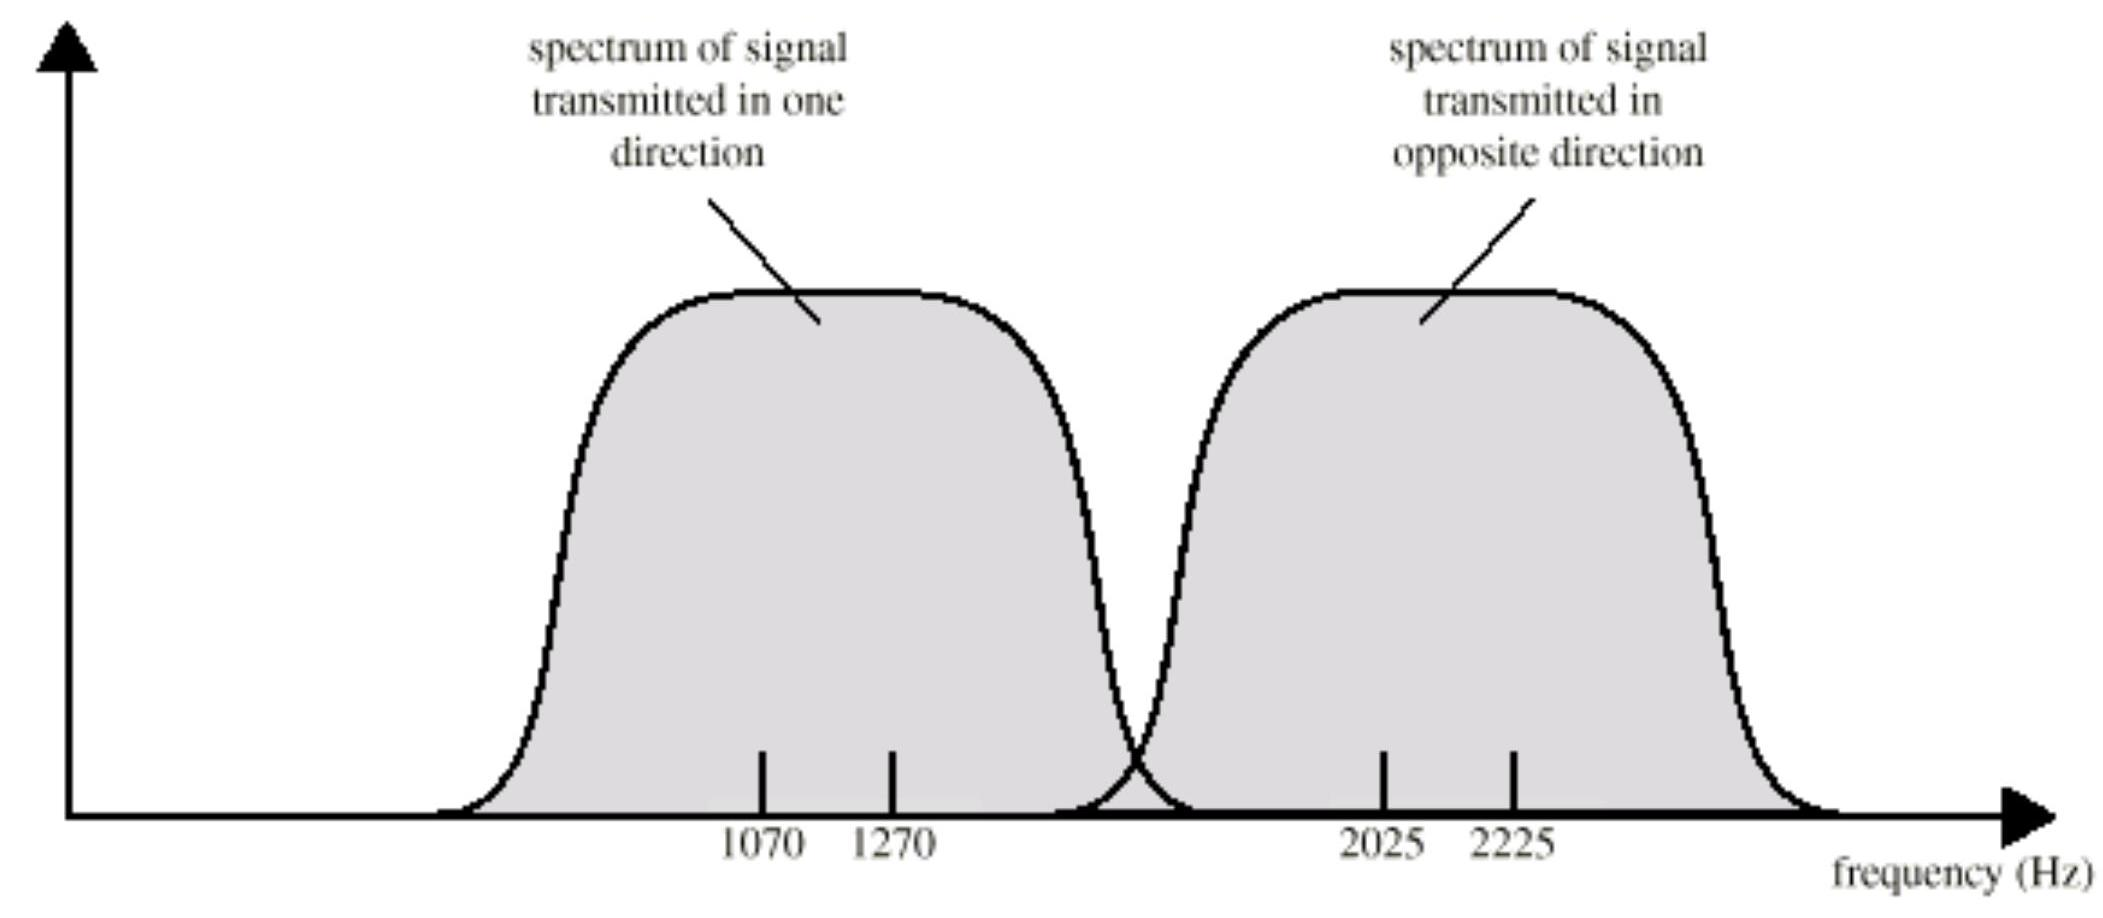
\includegraphics[max width=\textwidth]{2023_01_13_b07e3b4bcffdaab9792bg-072}
\end{center}

Figure 5.8 Full-Duplex FSK Transmission on a Voice-Grade Line


\os{newpage} item[{\rot\bf  Phase Shift Keying }]~\\[-3ex]

\bi
  \ite Phase of carrier signal is shifted to represent data - Binary PSK
\ei
\bi
 \ite Two phases represent two binary digits
 \ei


\bi
  \ite Differential PSK
\ei
\bi
 \ite Phase shifted relative to previous transmission rather than some reference signal
 \ei



\os{newpage} item[{\rot\bf  Differential PSK }]~\\[-3ex]

\begin{center}
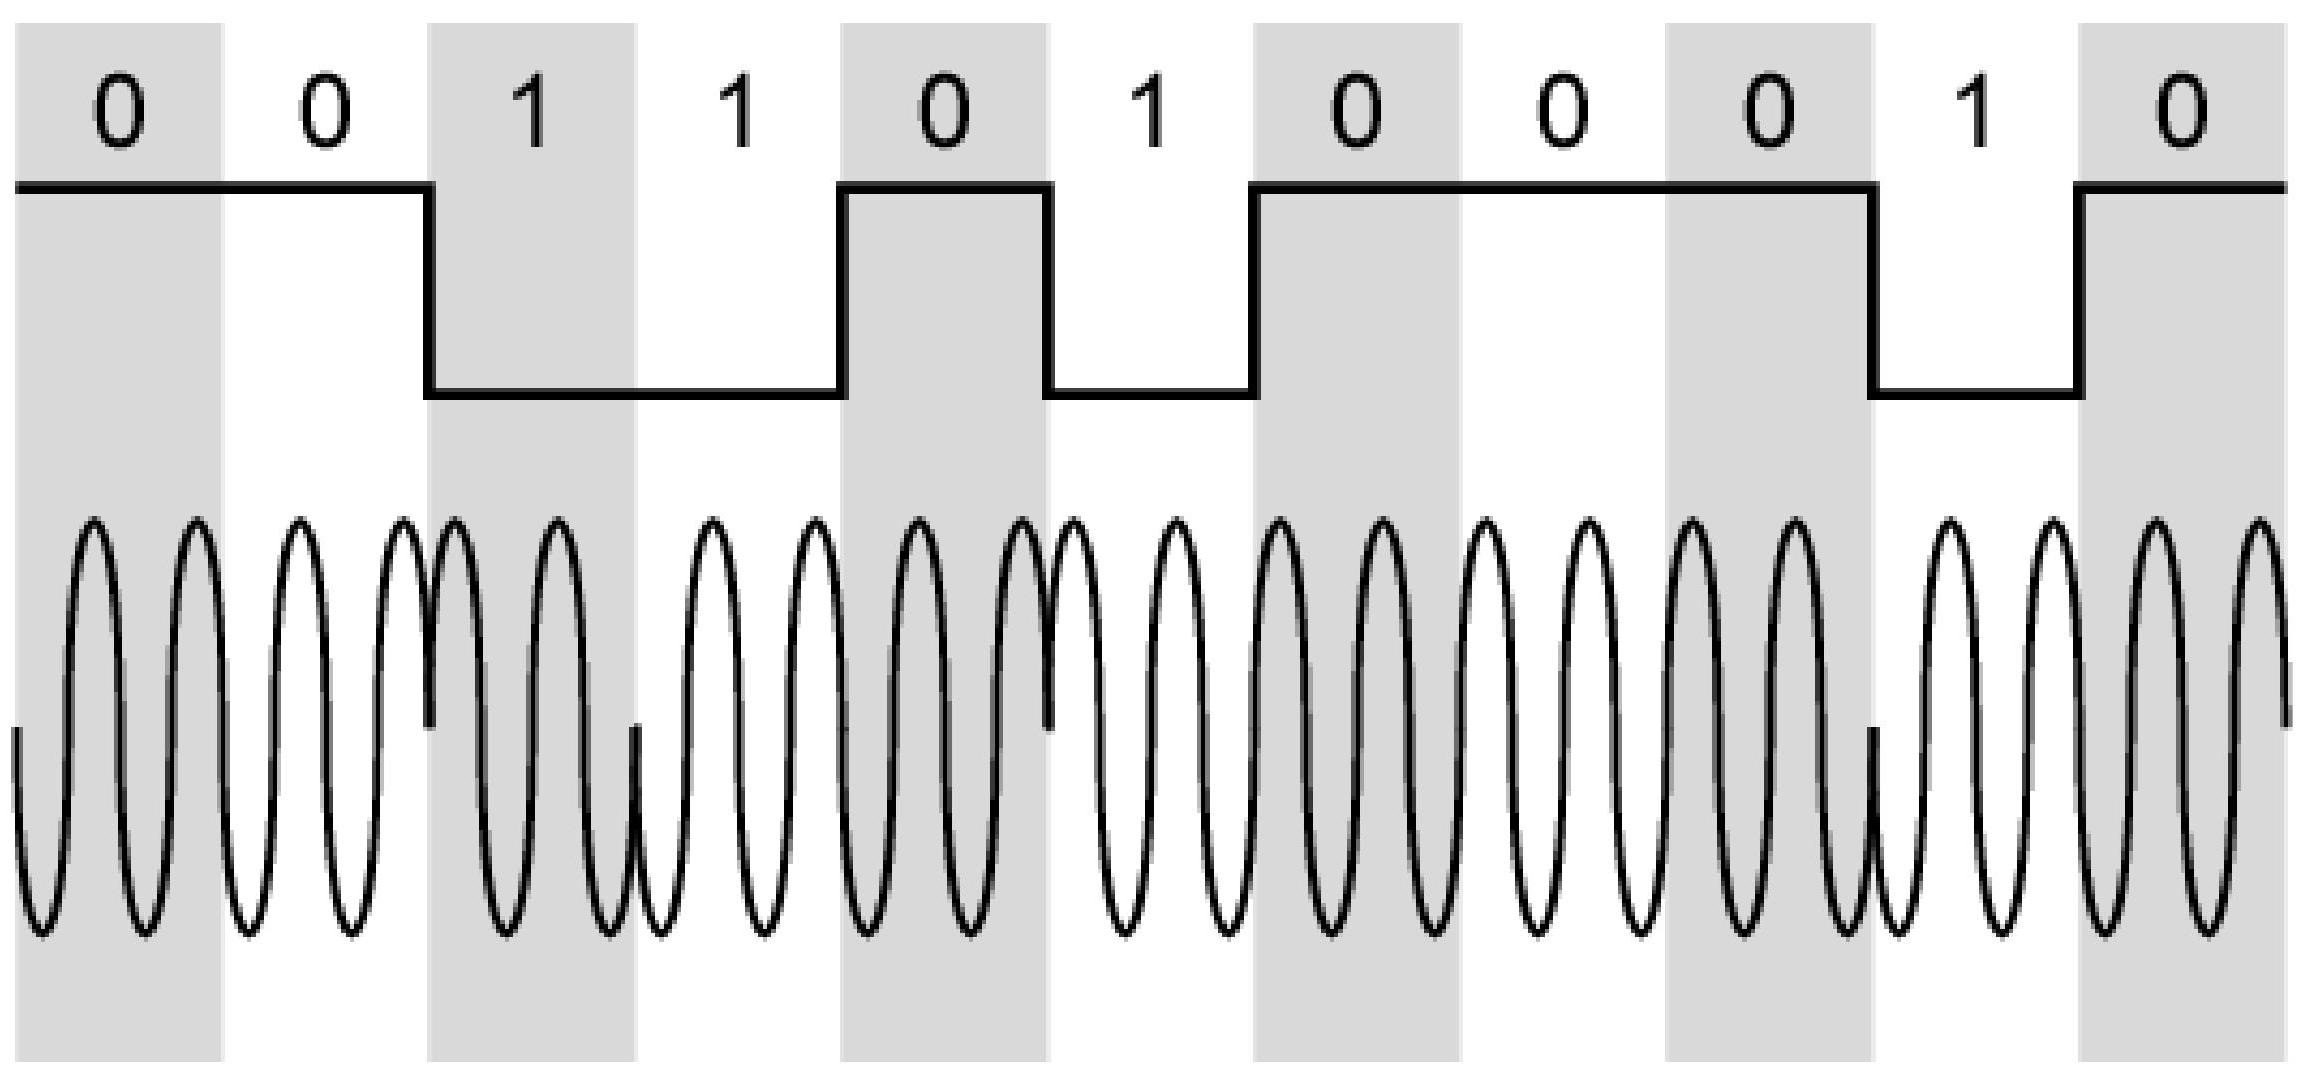
\includegraphics[max width=\textwidth]{2023_01_13_b07e3b4bcffdaab9792bg-074}
\end{center}


\os{newpage} item[{\rot\bf  Quadrature PSK }]~\\[-3ex]


\os{newpage} item[{\rot\bf  - More efficient use by each signal element representing more than one bit }]~\\[-3ex]
\bi
 \ite e.g. shifts of $\pi / 2\left(90^{\circ}\right)$
 \ei

\bi
 \ite Each element represents two bits
 \ei

\bi
 \ite Can use 8 phase angles and have more than one amplitude o $9600 b p s$ modem use 12 angles, four of which have two amplitudes
 \ei


\bi
  \ite Offset QPSK (orthogonal QPSK)
\ei
\bi
 \ite Delay in Q stream
 \ei



\os{newpage} item[{\rot\bf  QPSK and OQPSK Modulators }]~\\[-3ex]

$\mathrm{I}(\mathrm{t})$

R/2 bps

\begin{center}
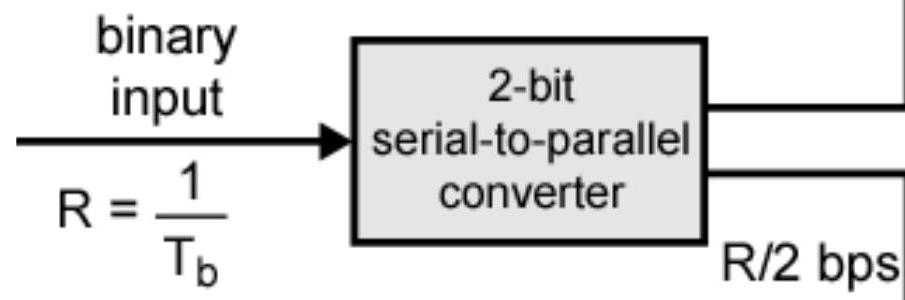
\includegraphics[max width=\textwidth]{2023_01_13_b07e3b4bcffdaab9792bg-076}
\end{center}

$a_{n}=\pm 1$

\begin{center}
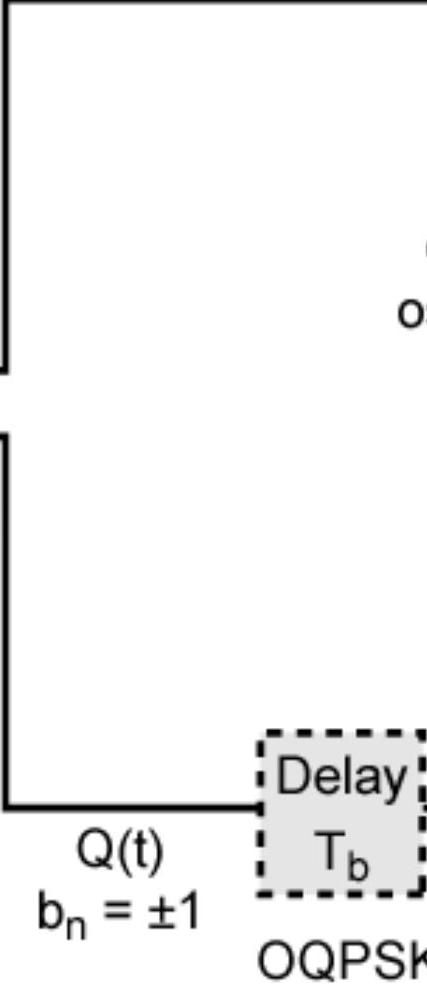
\includegraphics[max width=\textwidth]{2023_01_13_b07e3b4bcffdaab9792bg-076(1)}
\end{center}

only

\begin{center}
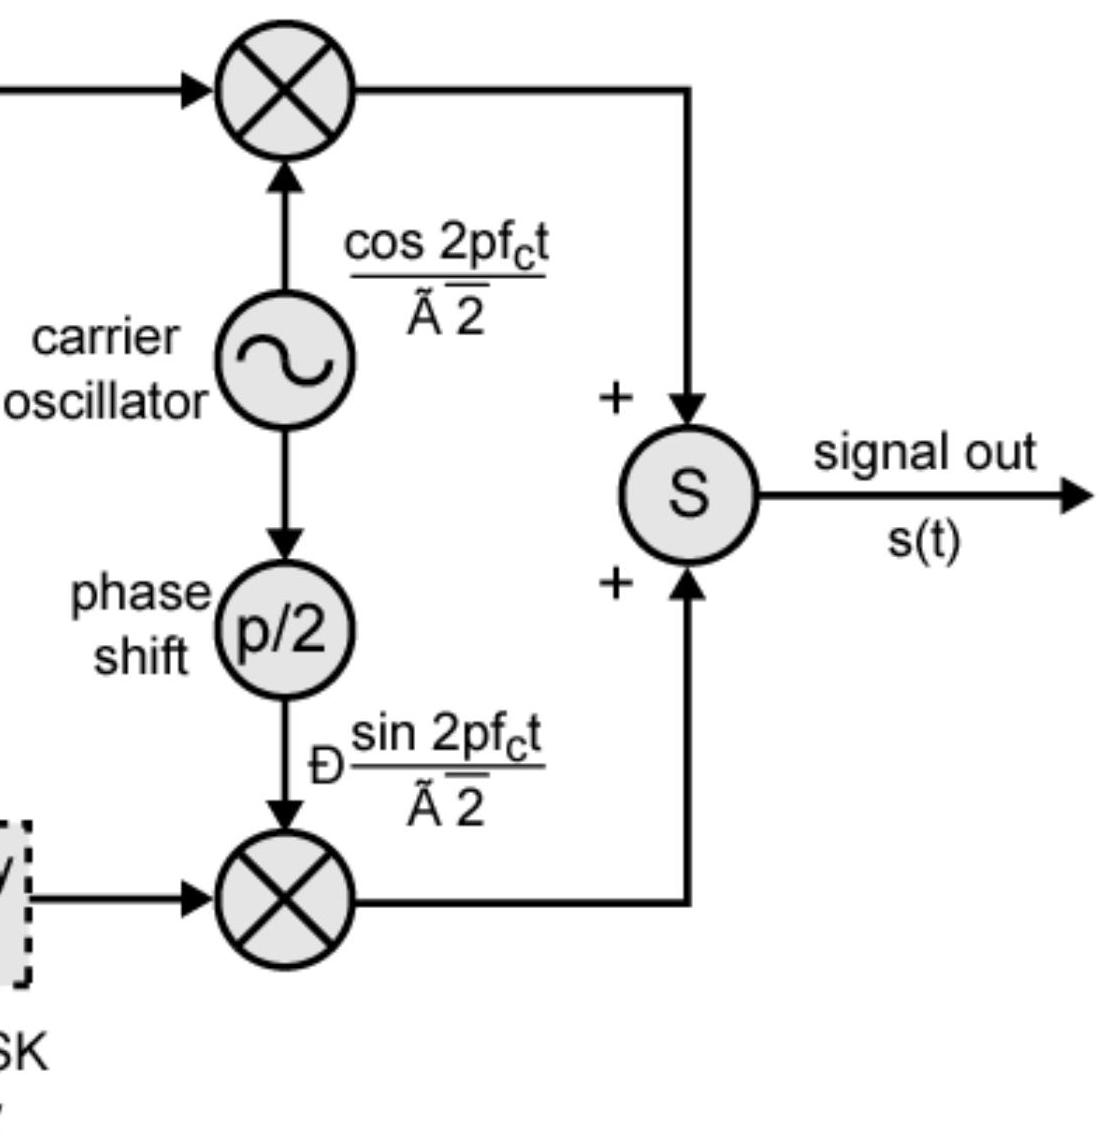
\includegraphics[max width=\textwidth]{2023_01_13_b07e3b4bcffdaab9792bg-076(2)}
\end{center}


\os{newpage} item[{\rot\bf  Examples of QPSF and OQPSK Waveforms }]~\\[-3ex]

\begin{center}
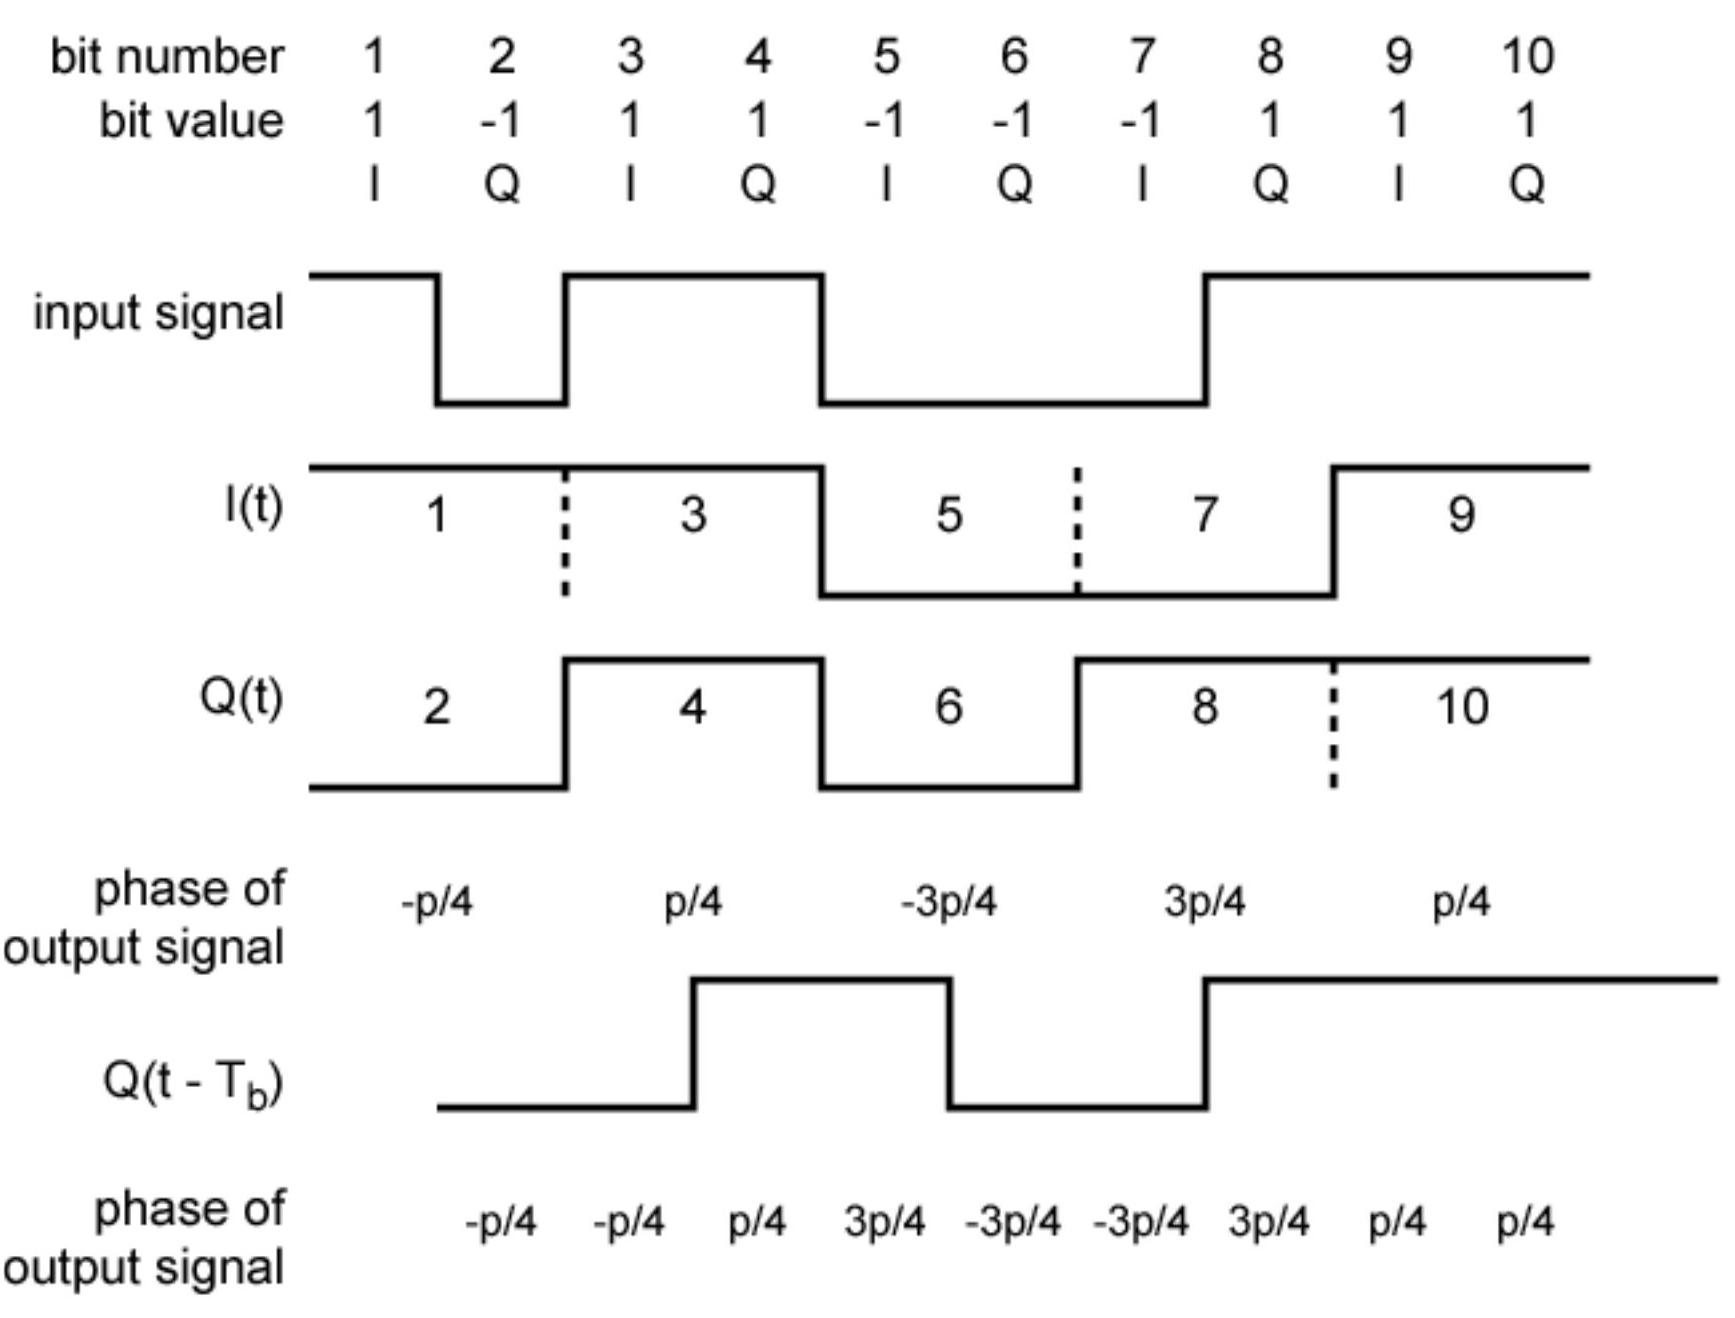
\includegraphics[max width=\textwidth]{2023_01_13_b07e3b4bcffdaab9792bg-077}
\end{center}


\os{newpage} item[{\rot\bf  Performance of Digital to Analog Modulation Schemes }]~\\[-3ex]

\bi
  \ite Bandwidth
\ei

ASK and PSK bandwidth directly related to bit rate

\bi
  \ite FSK bandwidth related to data rate for lower frequencies, but to offset of modulated frequency from carrier at high frequencies
\ei
\bi
 \ite (See Stallings for math)
 \ei


\bi
  \ite In the presence of noise, bit error rate of PSK and QPSK are about $3 \mathrm{~dB}$ superior to $\mathrm{ASK}$ and FSK
\ei


\os{newpage} item[{\rot\bf  Quadrature Amplitude Modulation }]~\\[-3ex]

\bi
  \ite QAM used on asymmetric digital subscriber line (ADSL) and some wireless

  \ite Combination of ASK and PSK

  \ite Logical extension of QPSK

  \ite Send two different signals simultaneously on same carrier frequency

  \ite Use two copies of carrier, one shifted $90^{\circ}$

\ei
\bi
 \ite Each carrier is ASK modulated
 \ei

\bi
 \ite Two independent signals over same medium
 \ei


\bi
  \ite Demodulate and combine for original binary output
\ei


\os{newpage} item[{\rot\bf  QAM Modulator }]~\\[-3ex]

\begin{center}
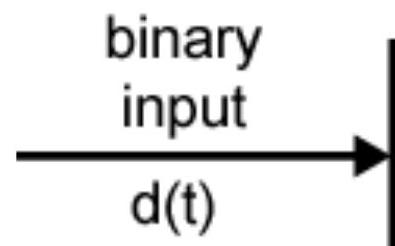
\includegraphics[max width=\textwidth]{2023_01_13_b07e3b4bcffdaab9792bg-080}
\end{center}

R bps

\begin{center}
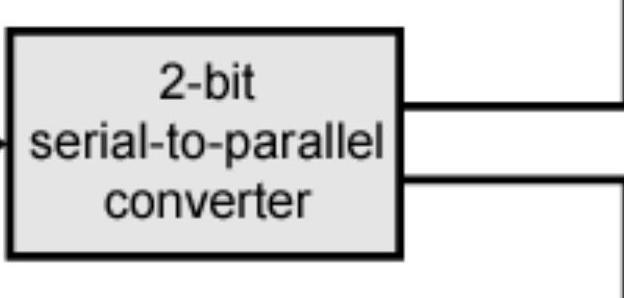
\includegraphics[max width=\textwidth]{2023_01_13_b07e3b4bcffdaab9792bg-080(1)}
\end{center}

$\mathrm{d}_{1}(\mathrm{t})$

R/2 bps

\begin{center}
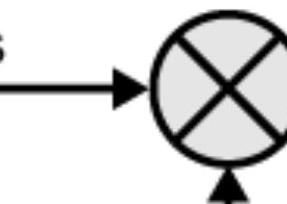
\includegraphics[max width=\textwidth]{2023_01_13_b07e3b4bcffdaab9792bg-080(2)}
\end{center}

$\int \cos 2 \mathrm{pf}_{\mathrm{c}} \mathrm{t}$
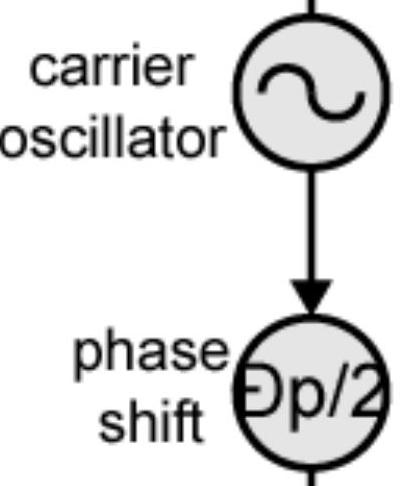
\includegraphics[max width=\textwidth, center]{2023_01_13_b07e3b4bcffdaab9792bg-080(3)}

QAM

signal out

$\begin{array}{r}d_{2}(t) \\ R / 2 \mathrm{bps} \\ \hline\end{array}$

$\begin{array}{r}\mathrm{d}_{2}(\mathrm{t}) \\ \mathrm{R} / 2 \mathrm{bps} \\ \hline\end{array}$

\begin{center}
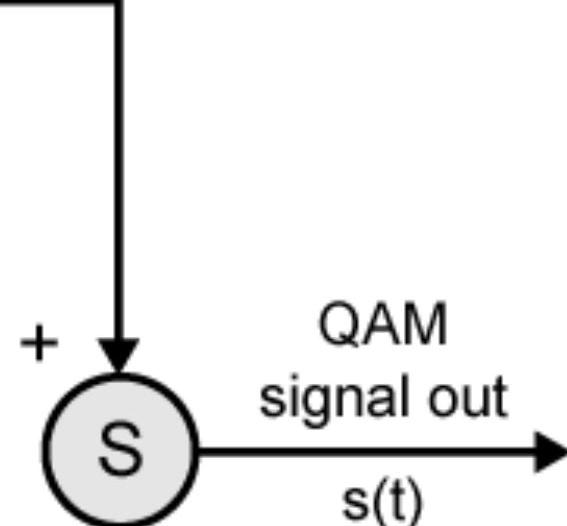
\includegraphics[max width=\textwidth]{2023_01_13_b07e3b4bcffdaab9792bg-080(4)}
\end{center}


\os{newpage} item[{\rot\bf  QAM Levels }]~\\[-3ex]

\bi
  \ite Two level ASK
\ei
\bi
 \ite Each of two streams in one of two states
 \ei

\bi
 \ite Four state system
 \ei

\bi
 \ite Essentially QPSK
 \ei


\bi
  \ite Four level ASK
\ei
\bi
 \ite Combined stream in one of 16 states
 \ei


\bi
  \ite 64 and 256 state systems have been implemented

  \ite Improved data rate for given bandwidth

\ei
\bi
 \ite Increased potential error rate
 \ei



\os{newpage} item[{\rot\bf  Analog Data, Digital Signal }]~\\[-3ex]

\bi
  \ite Digitization

  \ite Conversion of analog data into digital data

  \ite Digital data can then be transmitted using NRZ-L

  \ite Digital data can then be transmitted using code other than NRZ-L

  \ite Digital data can then be converted to analog signal

  \ite Analog to digital conversion done using a codec

  \ite Pulse code modulation

\ei
\bi
 \ite Delta modulation
 \ei



\os{newpage} item[{\rot\bf  Digitizing Analog Data }]~\\[-3ex]

\begin{center}
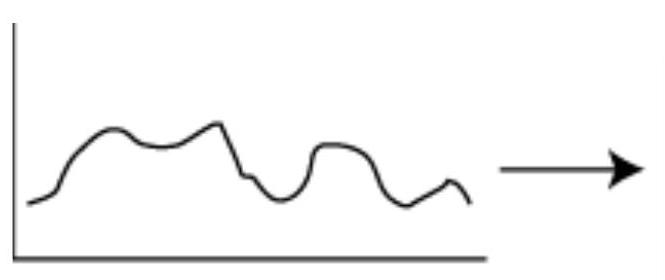
\includegraphics[max width=\textwidth]{2023_01_13_b07e3b4bcffdaab9792bg-083}
\end{center}

Analog data (voice)
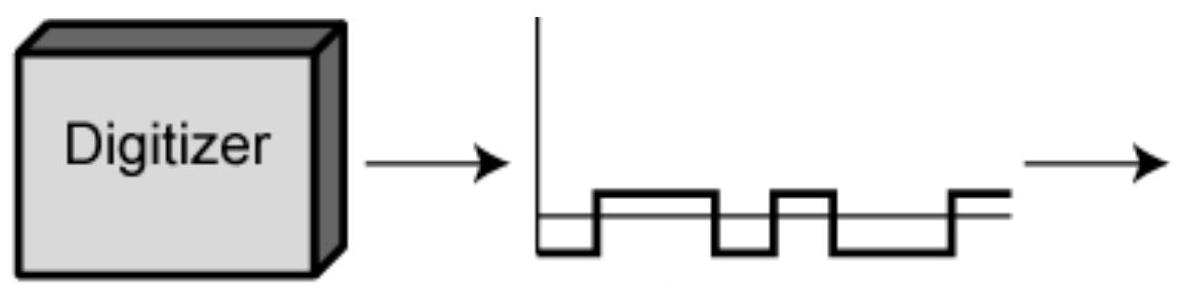
\includegraphics[max width=\textwidth, center]{2023_01_13_b07e3b4bcffdaab9792bg-083(1)}

Digital data

\begin{center}
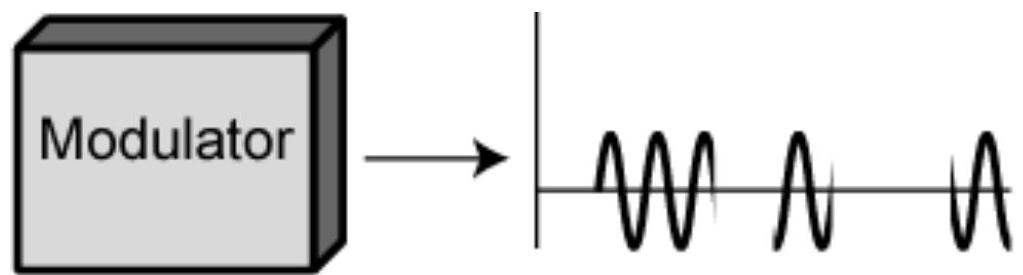
\includegraphics[max width=\textwidth]{2023_01_13_b07e3b4bcffdaab9792bg-083(2)}
\end{center}

Analog data

(ASK)


\os{newpage} item[{\rot\bf  Pulse Code Modulation(PCM) (1) }]~\\[-3ex]

\bi
  \ite If a signal is sampled at regular intervals at a rate higher than twice the highest signal frequency, the samples contain all the information of the original signal
\ei
\bi
 \ite (Proof - Stallings appendix 4A)
 \ei


\bi
  \ite Voice data limited to below $4000 \mathrm{~Hz}$

  \ite Require 80oo sample per second

  \ite Analog samples (Pulse Amplitude Modulation, PAM)

  \ite Each sample assigned digital value

\ei


\os{newpage} item[{\rot\bf  Pulse Code Modulation(PCM) (2) }]~\\[-3ex]

\bi
  \ite 4 bit system gives 16 levels

  \ite Quantized

\ei
\bi
 \ite Quantizing error or noise
 \ei

\bi
 \ite Approximations mean it is impossible to recover original exactly
 \ei


\bi
  \ite 8 bit sample gives 256 levels

  \ite Quality comparable with analog transmission

  \ite 8000 samples per second of 8 bits each gives $64 \mathrm{kbps}$

\ei


\os{newpage} item[{\rot\bf  PCM Example }]~\\[-3ex]

\begin{center}
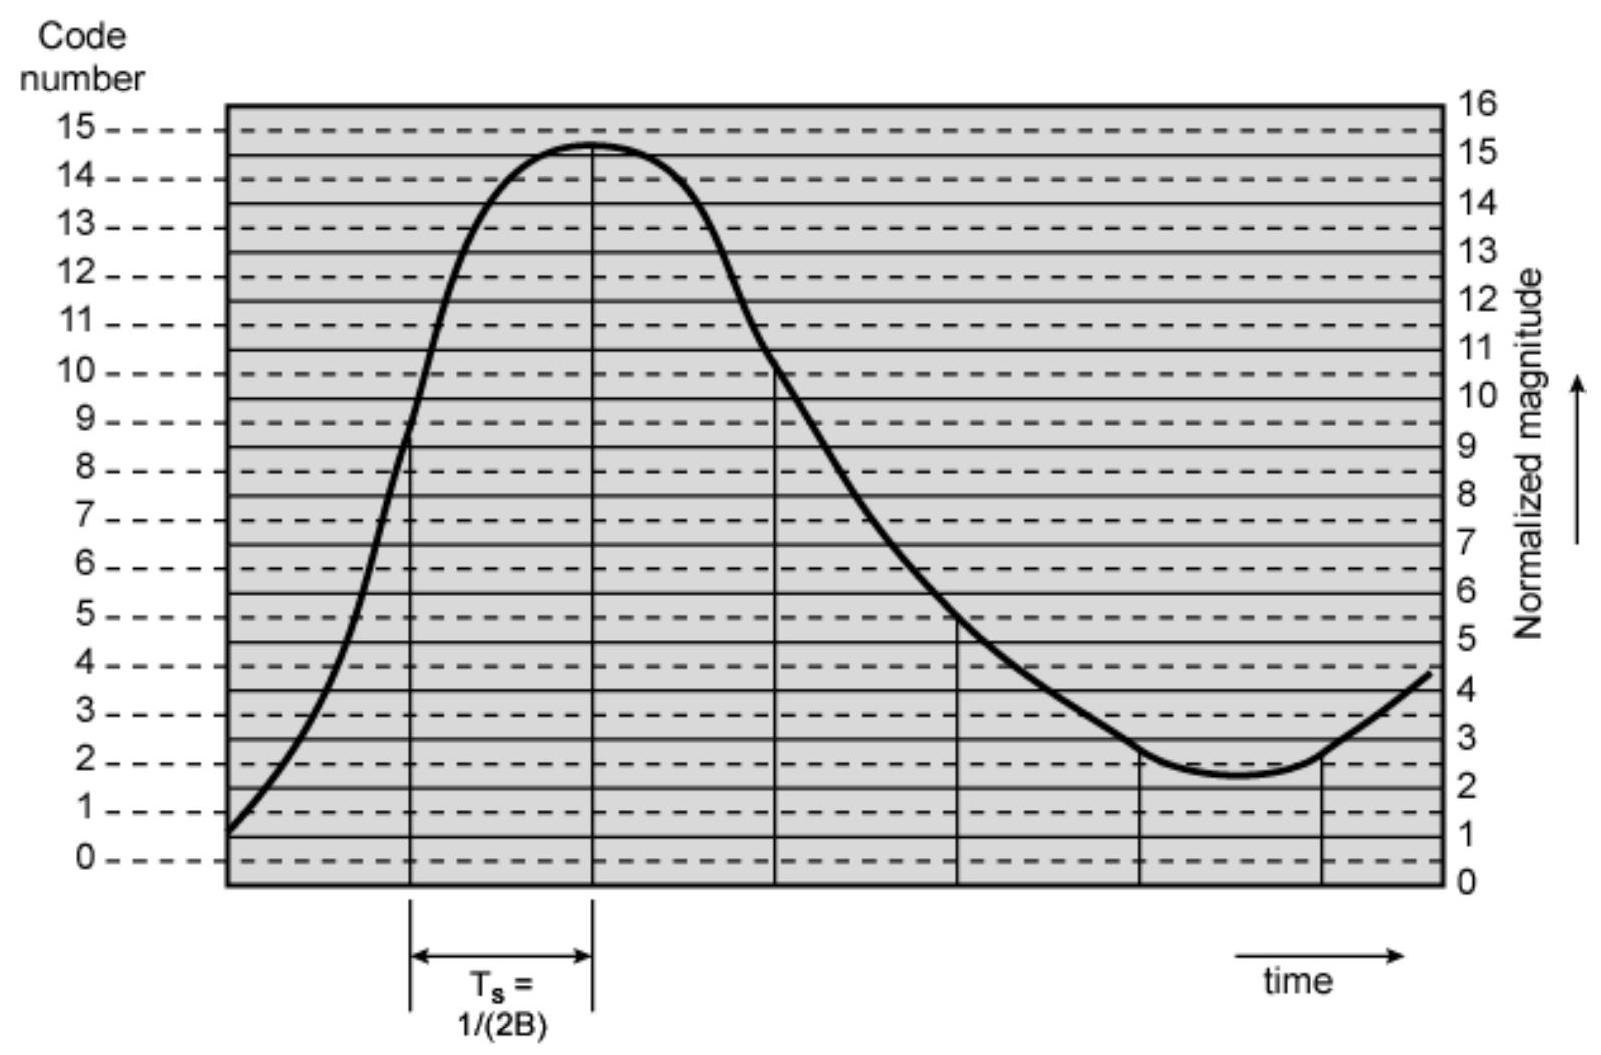
\includegraphics[max width=\textwidth]{2023_01_13_b07e3b4bcffdaab9792bg-086}
\end{center}

$\begin{array}{rccccccc}\text { PAM value } & 1.1 & 9.2 & 15.2 & 10.8 & 5.6 & 2.8 & 2.7 \\ \text { quantized code number } & 1 & 9 & 15 & 10 & 5 & 2 & 2 \\ \text { PCM code } & 0001 & 1001 & 1111 & 1010 & 0101 & 0010 & 0010\end{array}$


\os{newpage} item[{\rot\bf  PCM Block Diagram }]~\\[-3ex]

Continuous-time, continuous amplitud (analog) input signal

\begin{center}
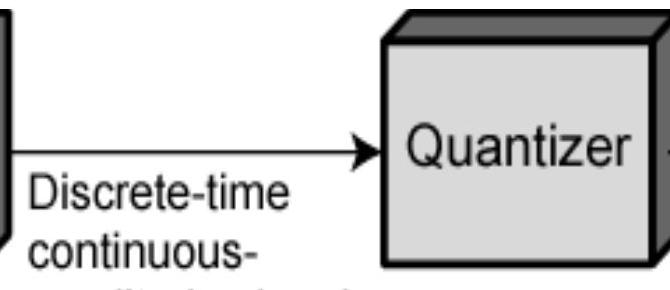
\includegraphics[max width=\textwidth]{2023_01_13_b07e3b4bcffdaab9792bg-087}
\end{center}

amplitude signal

(PAM pulses)

\begin{center}
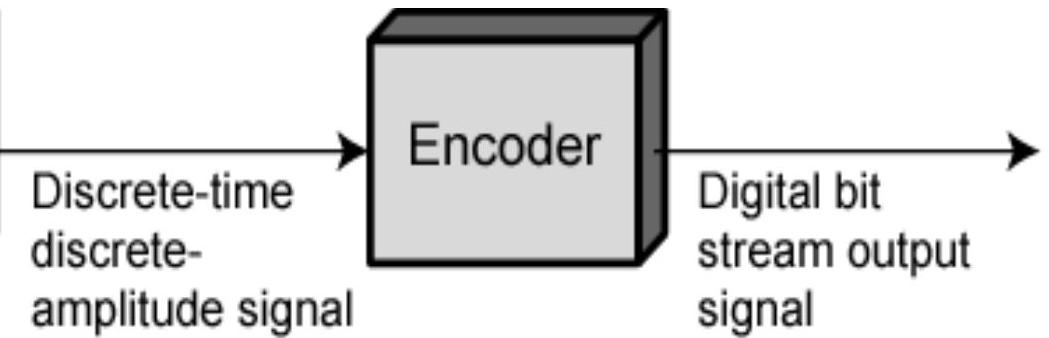
\includegraphics[max width=\textwidth]{2023_01_13_b07e3b4bcffdaab9792bg-087(1)}
\end{center}

(PCM pulses)


\os{newpage} item[{\rot\bf  Nonlinear Encoding }]~\\[-3ex]

\bi
  \ite Quantization levels not evenly spaced

  \ite Reduces overall signal distortion

  \ite Can also be done by companding

\ei


\os{newpage} item[{\rot\bf  Effect of Non-Linear Coding }]~\\[-3ex]

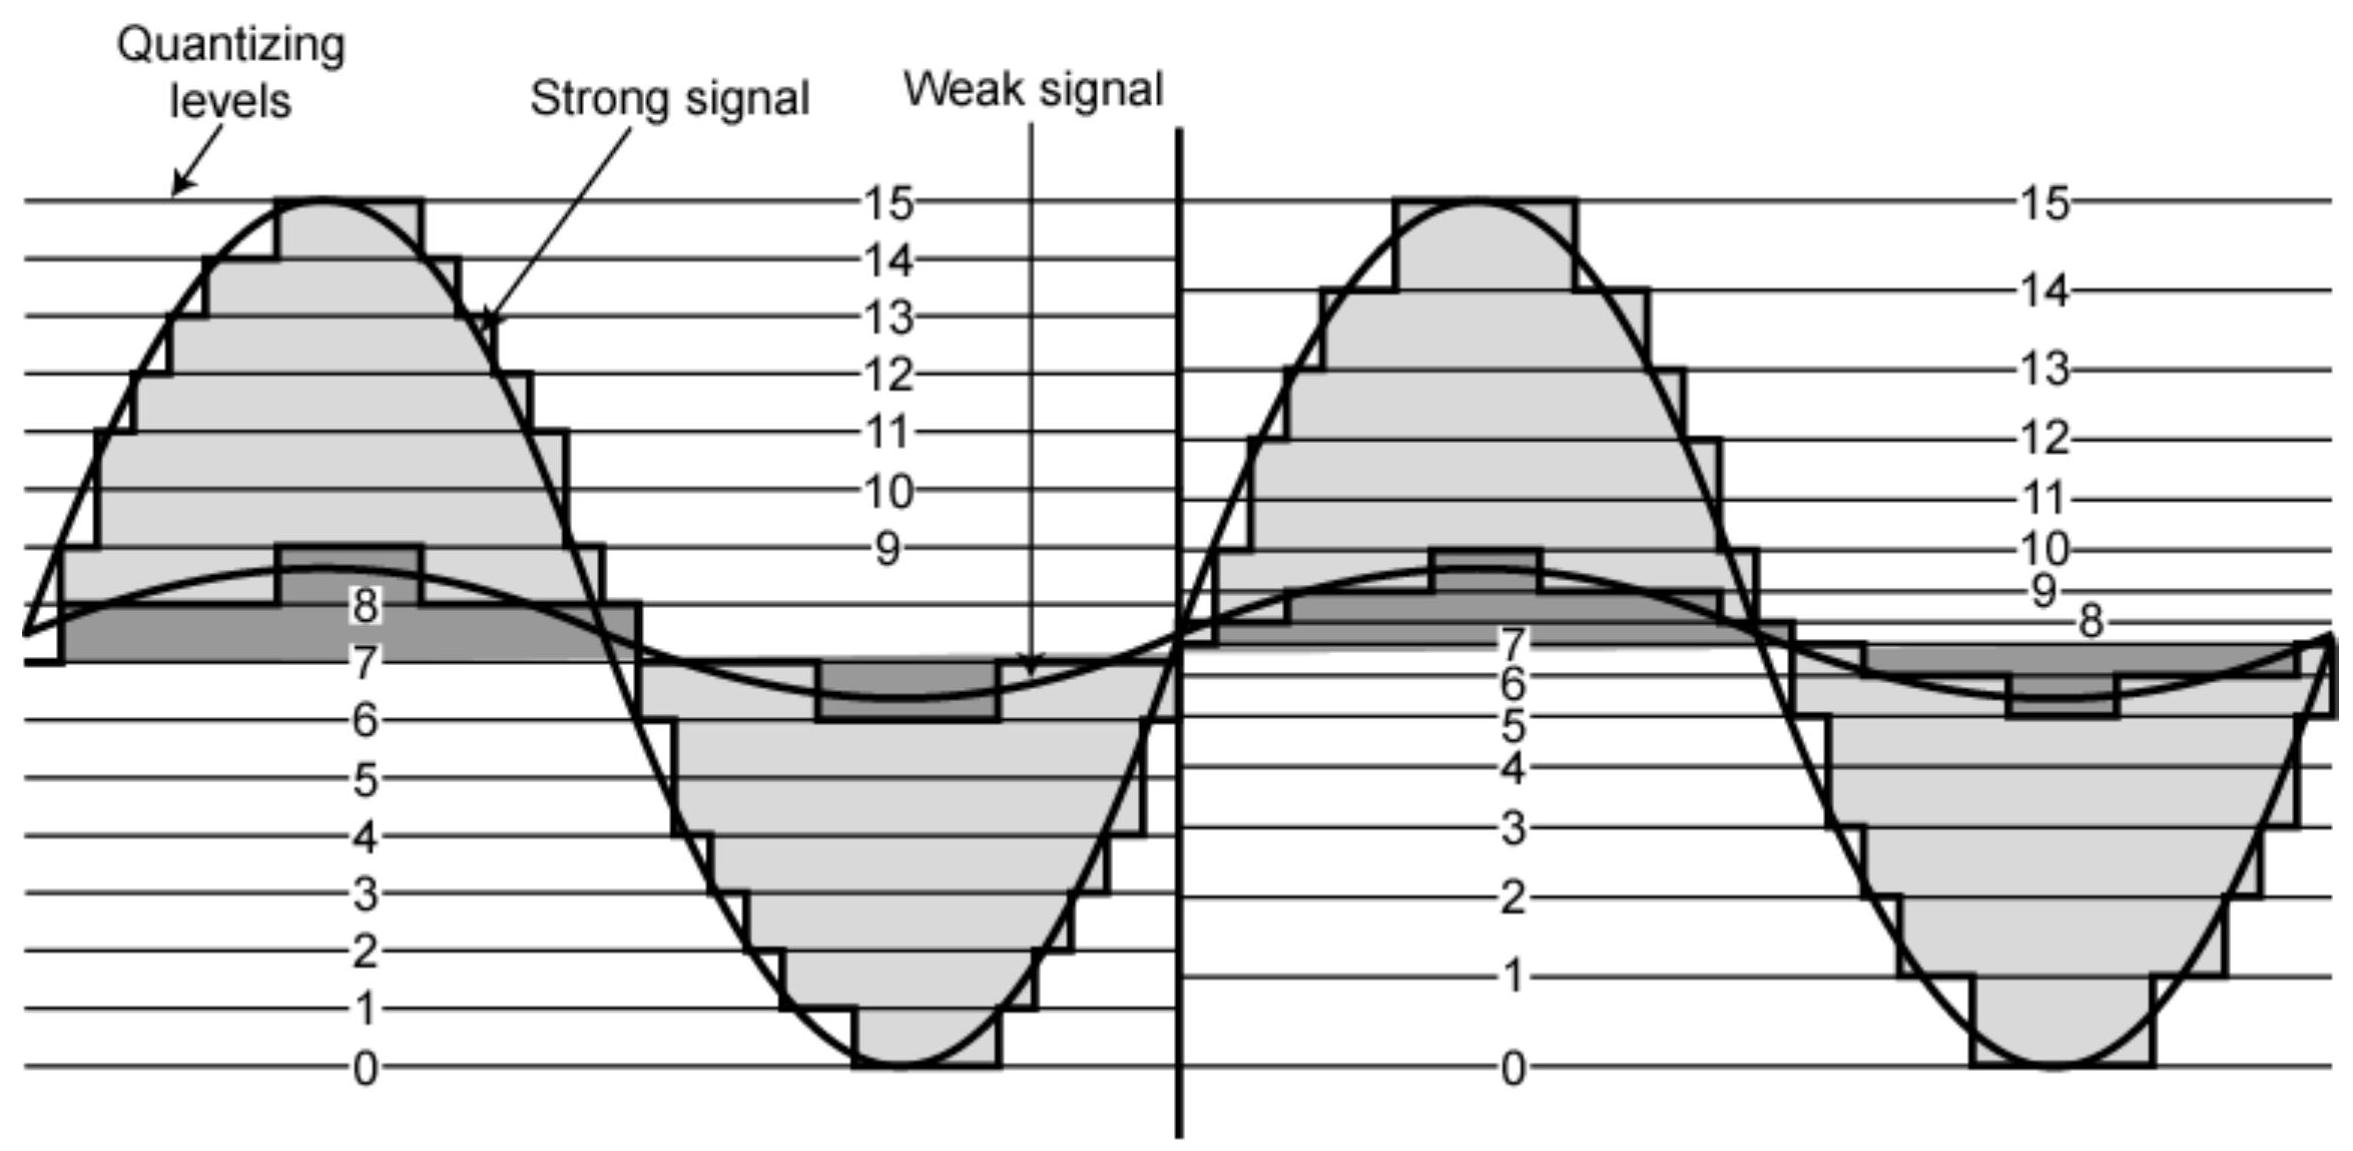
\includegraphics[max width=\textwidth, center]{2023_01_13_b07e3b4bcffdaab9792bg-089}
(a) Without nonlinear encoding
(b) With nonlinear encoding


\os{newpage} item[{\rot\bf  Typical Companding Functions }]~\\[-3ex]

\begin{center}
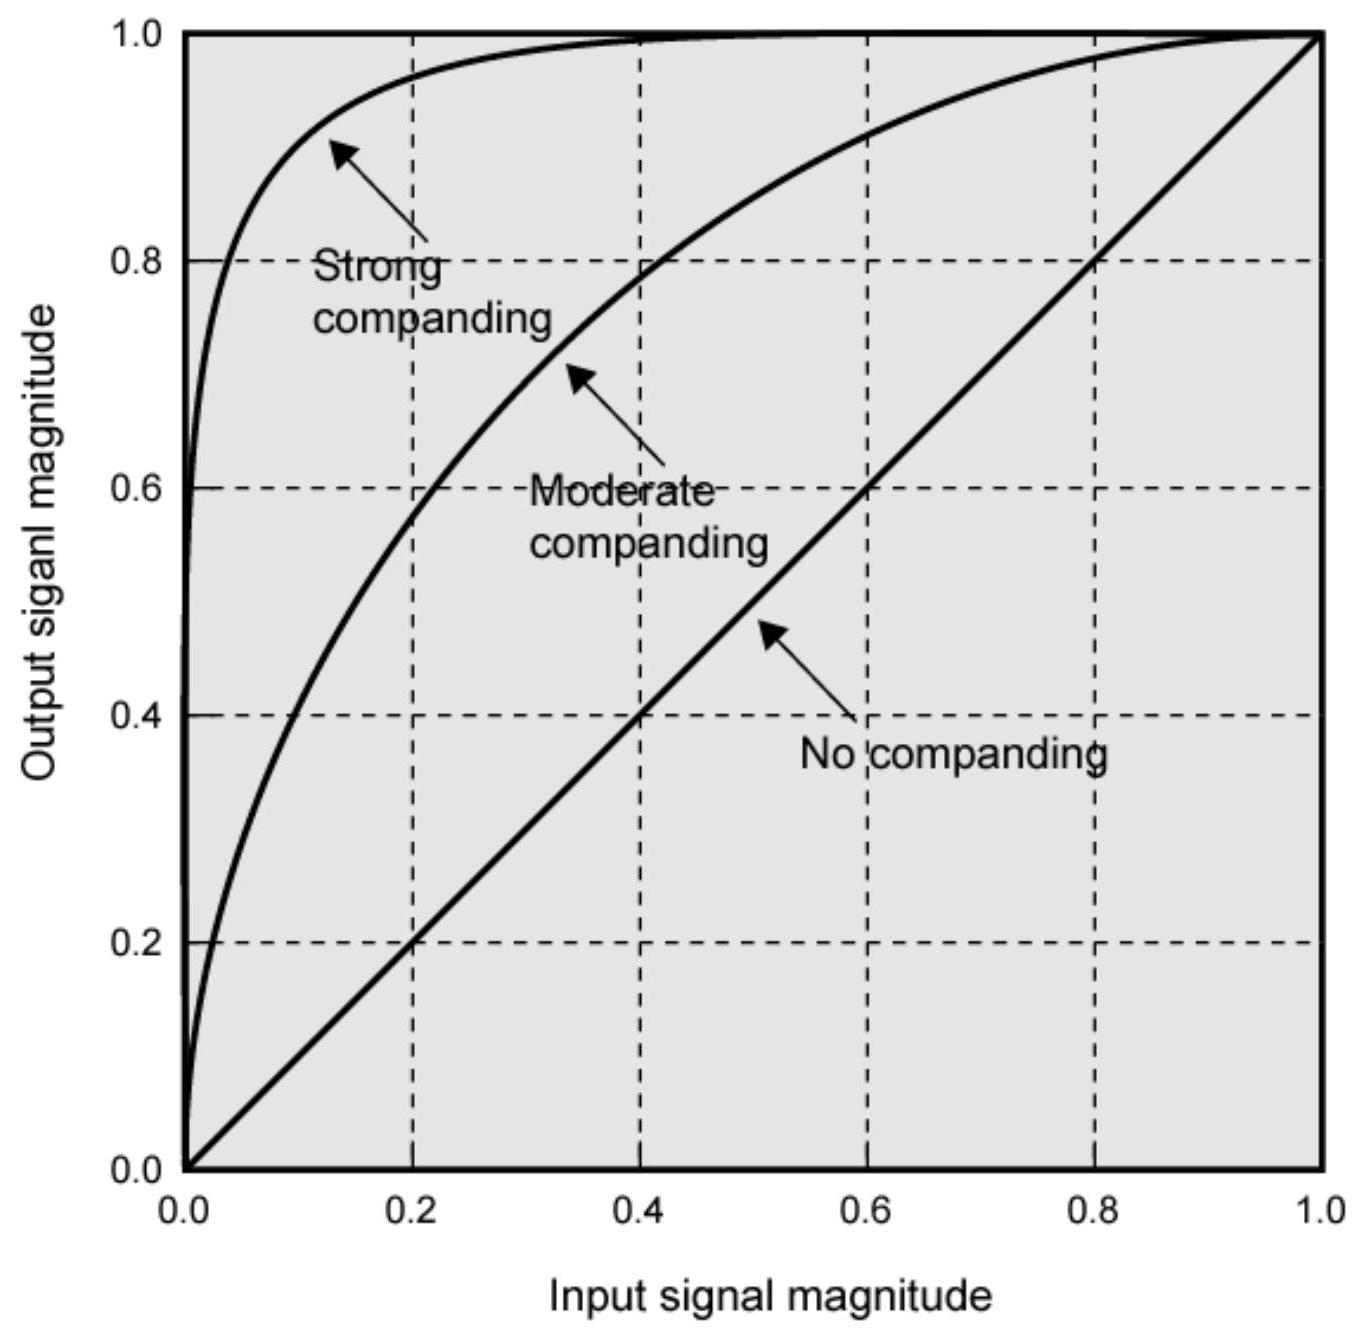
\includegraphics[max width=\textwidth]{2023_01_13_b07e3b4bcffdaab9792bg-090}
\end{center}


\os{newpage} item[{\rot\bf  Delta Modulation }]~\\[-3ex]

\bi
  \ite Analog input is approximated by a staircase function

  \ite Move up or down one level ( $\delta$ ) at each sample interval

  \ite Binary behavior

  \ite Function moves up or down at each sample interval

\ei


\os{newpage} item[{\rot\bf  Delta Modulation - example }]~\\[-3ex]

\begin{center}
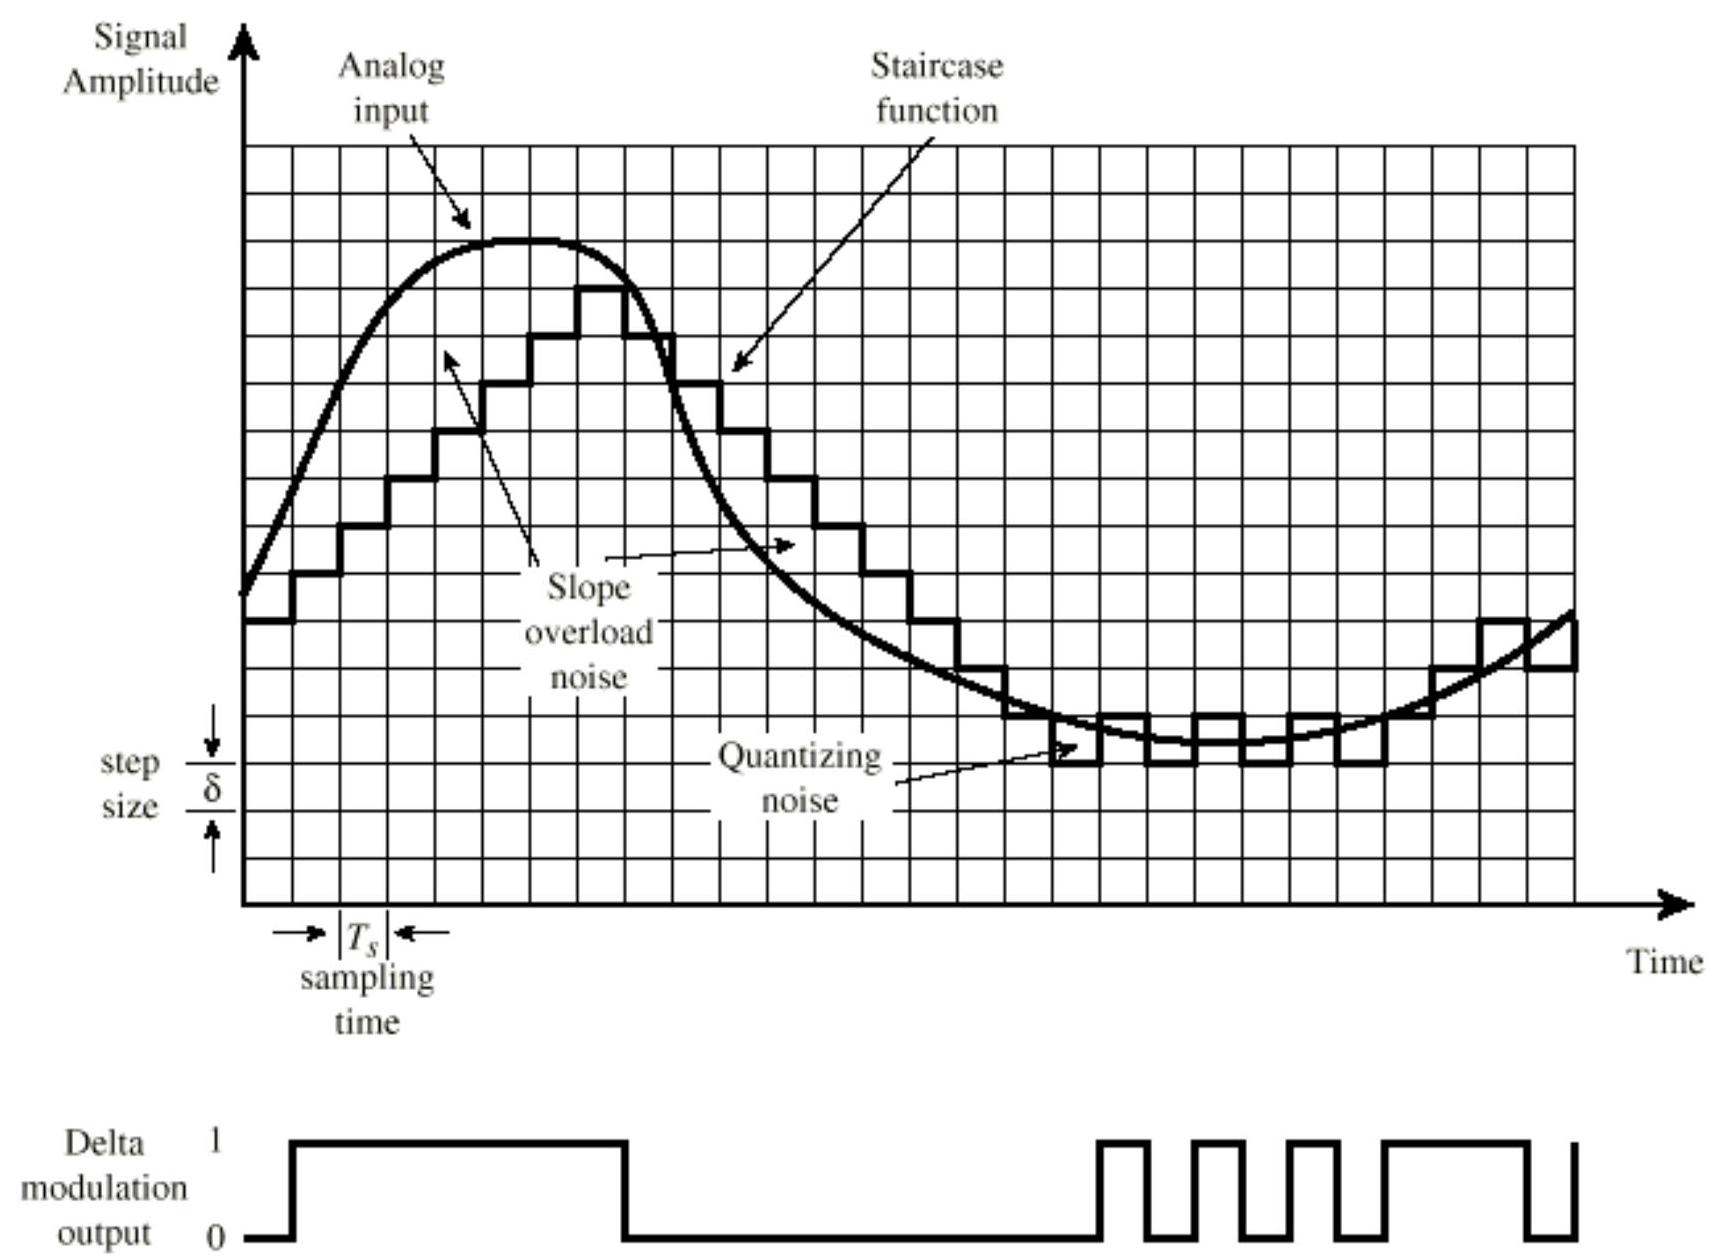
\includegraphics[max width=\textwidth]{2023_01_13_b07e3b4bcffdaab9792bg-092}
\end{center}


\os{newpage} item[{\rot\bf  Delta Modulation - Operation }]~\\[-3ex]

\begin{center}
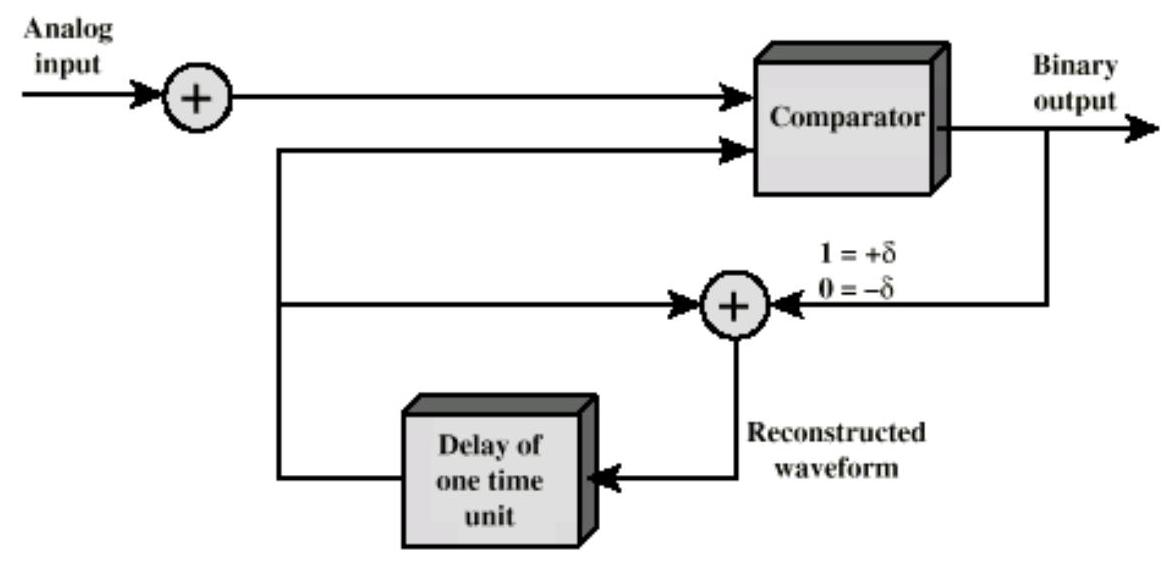
\includegraphics[max width=\textwidth]{2023_01_13_b07e3b4bcffdaab9792bg-093}
\end{center}

(a) Transmission

\begin{center}
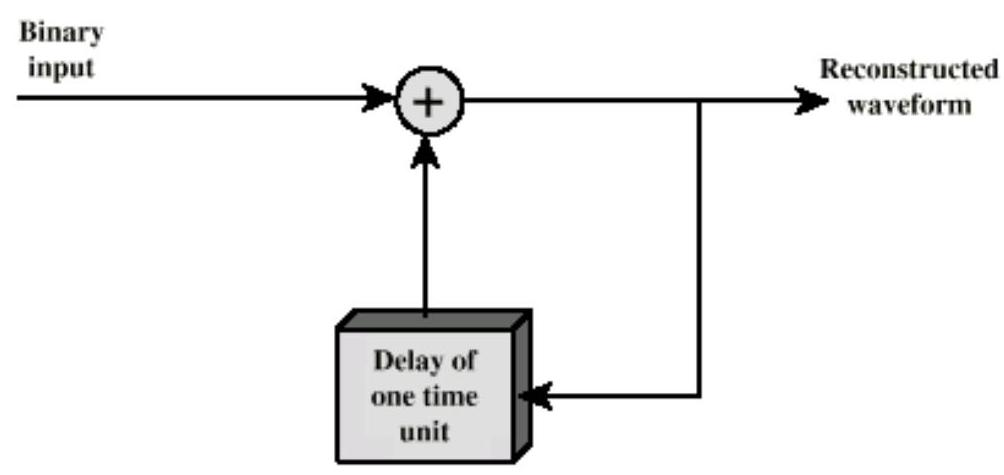
\includegraphics[max width=\textwidth]{2023_01_13_b07e3b4bcffdaab9792bg-093(1)}
\end{center}

(b) Reception


\os{newpage} item[{\rot\bf  Delta Modulation - Performance }]~\\[-3ex]

\bi
  \ite Good voice reproduction

  \ite PCM - 128 levels (7 bit)

\ei
\bi
 \ite Voice bandwidth $4 \mathrm{khz}$
 \ei

\bi
 \ite Should be $8000 \times 7=56 \mathrm{kbps}$ for PCM
 \ei


\bi
  \ite Data compression can improve on this
\ei
\bi
 \ite e.g. Interframe coding techniques for video
 \ei



\os{newpage} item[{\rot\bf  Analog Data, Analog Signals }]~\\[-3ex]

\bi
  \ite Why modulate analog signals?

  \ite Higher frequency can give more efficient transmission

  \ite Permits frequency division multiplexing (chapter 8)

  \ite Types of modulation

  \ite Amplitude

  \ite Frequency

\ei
\bi
 \ite Phase
 \ei



\os{newpage} item[{\rot\bf  Analog Modulation }]~\\[-3ex]

\begin{center}
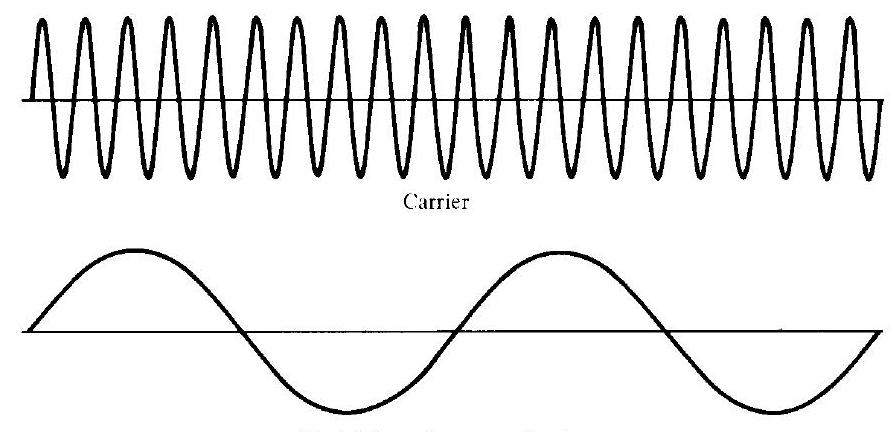
\includegraphics[max width=\textwidth]{2023_01_13_b07e3b4bcffdaab9792bg-096}
\end{center}

Modulating sine-wave signal

\begin{center}
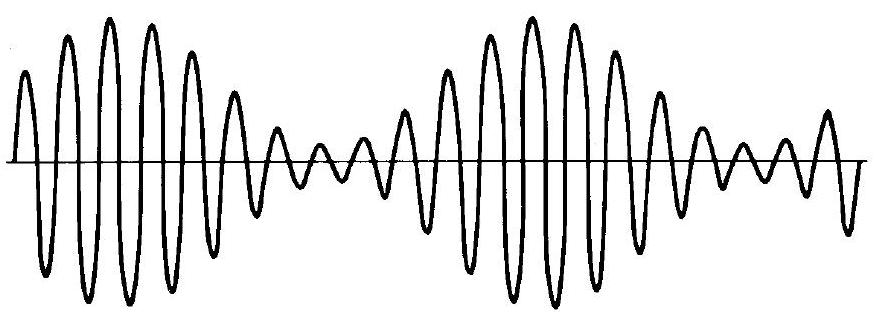
\includegraphics[max width=\textwidth]{2023_01_13_b07e3b4bcffdaab9792bg-096(1)}
\end{center}

Amplitude-modulated (DSBTC) wave

\begin{center}
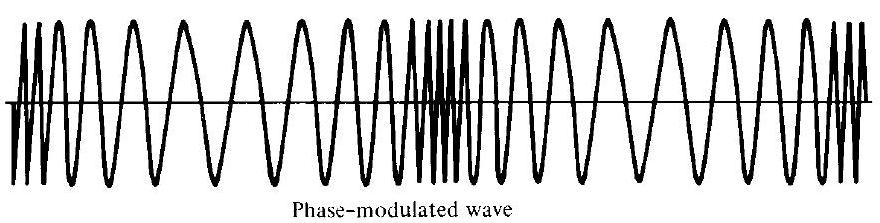
\includegraphics[max width=\textwidth]{2023_01_13_b07e3b4bcffdaab9792bg-096(2)}
\end{center}

Phase-modulated wave

\begin{center}
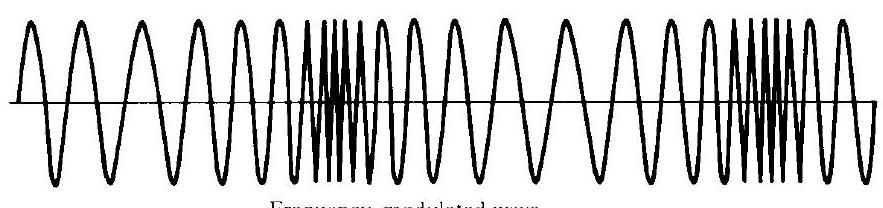
\includegraphics[max width=\textwidth]{2023_01_13_b07e3b4bcffdaab9792bg-096(3)}
\end{center}


\os{newpage} item[{\rot\bf  Ethernet }]~\\[-3ex]


\os{newpage} item[{\rot\bf  Ethernet }]~\\[-3ex]

\bi
  \ite Most successful local area networking technology of last 20 years.

  \ite Developed in the mid-1970s by researchers at the Xerox Palo Alto Research Centers (PARC).

  \ite Uses CSMA/CD technology

  \ite Carrier Sense Multiple Access with Collision Detection.

  \ite A set of nodes send and receive frames over a shared link.

  \ite Carrier sense means that all nodes can distinguish between an idle and a busy link.

  \ite Collision detection means that a node listens as it transmits and can therefore detect when a frame it is transmitting has collided with a frame transmitted by another node.

\ei


\os{newpage} item[{\rot\bf  Ethernet }]~\\[-3ex]

\bi
  \ite Uses ALOHA (packet radio network) as the root protocol

  \ite Developed at the University of Hawaii to support communication across the Hawaiian Islands.

  \ite For ALOHA the medium was atmosphere, for Ethernet the medium is a coax cable.

  \ite DEC and Intel joined Xerox to define a 10-Mbps Ethernet standard in 1978.

  \ite This standard formed the basis for IEEE standard 802.3

  \ite More recently 802.3 has been extended to include a 100Mbps version called Fast Ethernet and a 1000-Mbps version called Gigabit Ethernet.

\ei


\os{newpage} item[{\rot\bf  Ethernet }]~\\[-3ex]

\bi
  \ite An Ethernet segment is implemented on a coaxial cable of up to $500 \mathrm{~m}$.

  \ite This cable is similar to the type used for cable TV except that it typically has an impedance of 50 ohms instead of cable TV's 75 ohms.

  \ite Hosts connect to an Ethernet segment by tapping into it.

  \ite A transceiver (a small device directly attached to the tap) detects when the line is idle and drives signal when the host is transmitting.

  \ite The transceiver also receives incoming signal.

  \ite The transceiver is connected to an Ethernet adaptor which is plugged into the host.

  \ite The protocol is implemented on the adaptor.

\ei


\os{newpage} item[{\rot\bf  Ethernet }]~\\[-3ex]

Transceiver

\begin{center}

\includegraphics[max width=\textwidth]{2023_01_13_b07e3b4bcffdaab9792bg-101}
\end{center}

Adaptor

Host


\os{newpage} item[{\rot\bf  Ethernet transceiver and adaptor }]~\\[-3ex]


\os{newpage} item[{\rot\bf  Ethernet }]~\\[-3ex]

\bi
  \ite Multiple Ethernet segments can be joined together by repeaters.

  \ite A repeater is a device that forwards digital signals.

  \ite No more than four repeaters may be positioned between any pair of hosts.

\ei
\bi
 \ite An Ethernet has a total reach of only $2500 \mathrm{~m}$.
 \ei



\os{newpage} item[{\rot\bf  Ethernet - Repeater }]~\\[-3ex]

\begin{center}
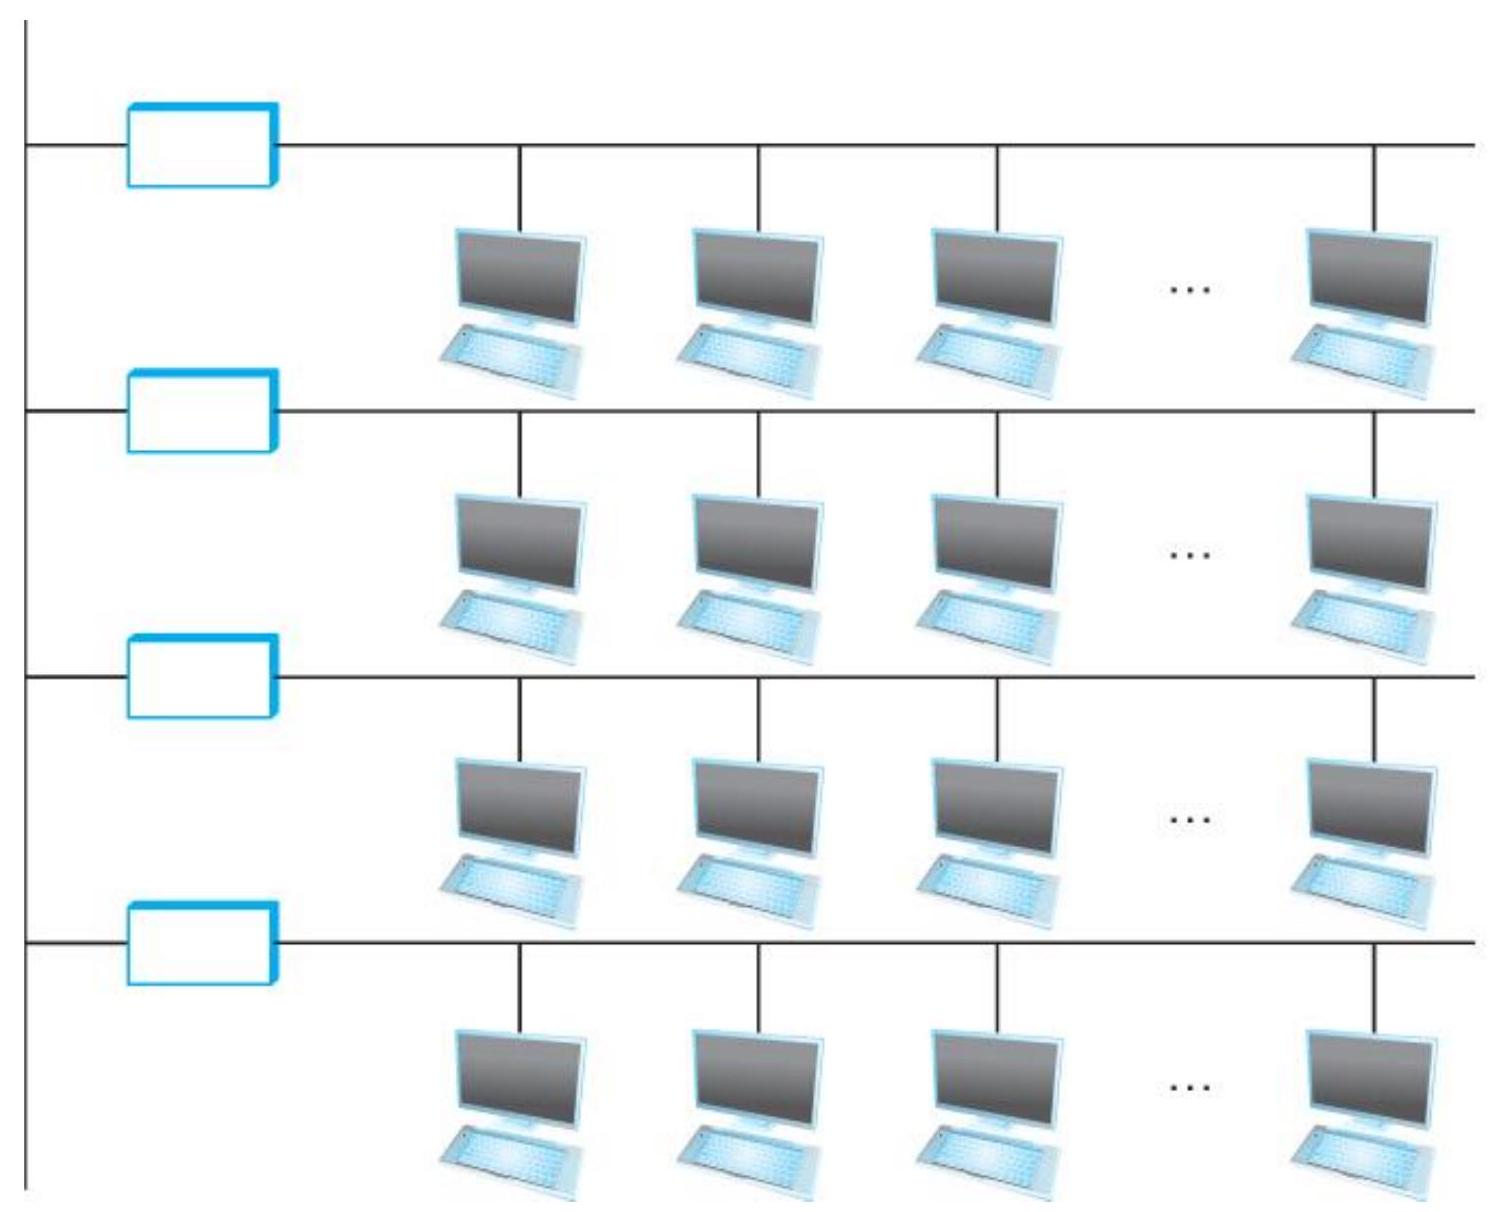
\includegraphics[max width=\textwidth]{2023_01_13_b07e3b4bcffdaab9792bg-103}
\end{center}

\begin{center}

\includegraphics[max width=\textwidth]{2023_01_13_b07e3b4bcffdaab9792bg-103(1)}
\end{center}

Repeater

\begin{center}
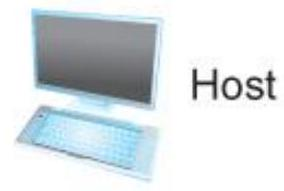
\includegraphics[max width=\textwidth]{2023_01_13_b07e3b4bcffdaab9792bg-103(2)}
\end{center}


\os{newpage} item[{\rot\bf  Ethernet }]~\\[-3ex]

\bi
  \ite Any signal placed on the Ethernet by a host is broadcast over the entire network
\ei
\bi
 \ite Signal is propagated in both directions.
 \ei

\bi
 \ite Repeaters forward the signal on all outgoing segments.
 \ei

\bi
 \ite Terminators attached to the end of each segment absorb the signal.
 \ei


\bi
  \ite Ethernet uses Manchester encoding scheme.
\ei


\os{newpage} item[{\rot\bf  Ethernet }]~\\[-3ex]

\bi
  \ite New Technologies in Ethernet

  \ite Instead of using coax cable, an Ethernet can be constructed from a thinner cable known as 10 Base2 (the original was 10Base5)

\ei

10 means the network operates at $10 \mathrm{Mbps}$

· Base means the cable is used in a baseband system

$\times 2$ means that a given segment can be no longer than $200 \mathrm{~m}$


\os{newpage} item[{\rot\bf  Ethernet }]~\\[-3ex]

\bi
  \ite New Technologies in Ethernet - Another cable technology is 10BaseT
\ei

\begin{CJK}{UTF8}{mj}乂\end{CJK} T stands for twisted pair

\bi
  \ite Limited to $100 \mathrm{~m}$ in length
\ei
\bi
 \ite With 10 BaseT, the common configuration is to have several point to point segments coming out of a multiway repeater, called $H u b$
 \ei



\os{newpage} item[{\rot\bf  Ethernet }]~\\[-3ex]

\begin{center}
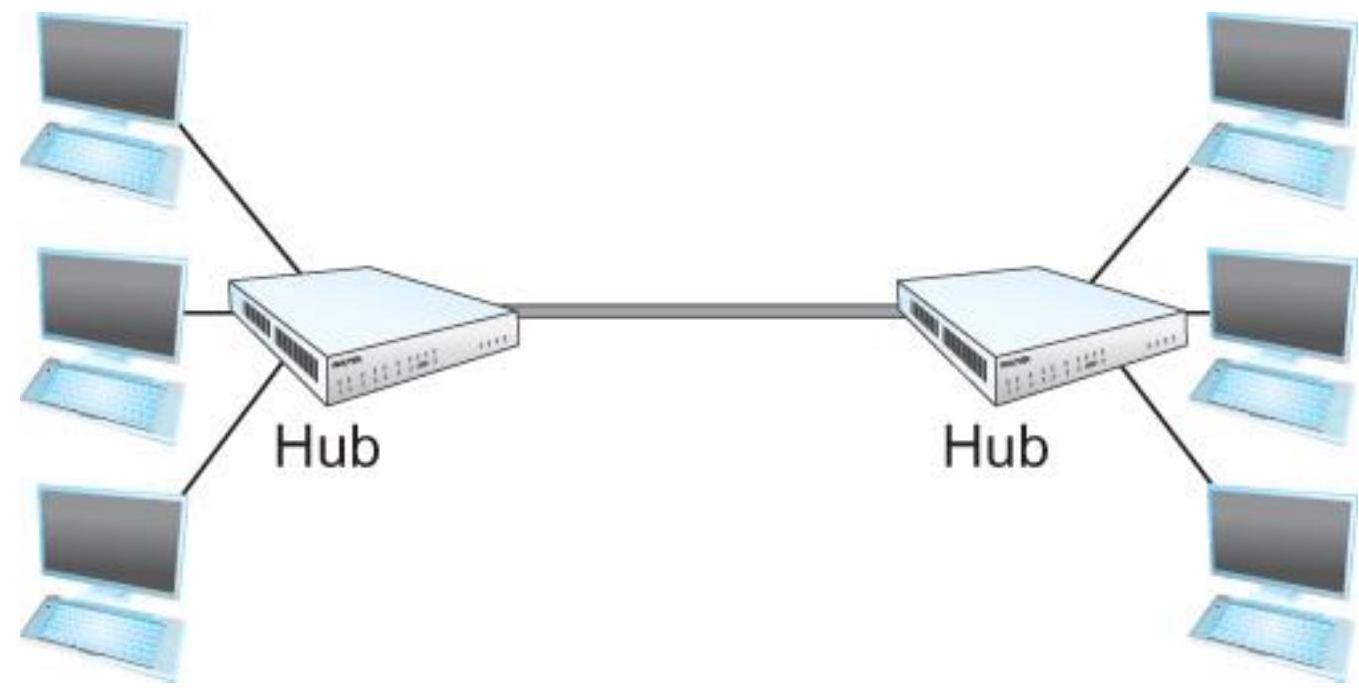
\includegraphics[max width=\textwidth]{2023_01_13_b07e3b4bcffdaab9792bg-107}
\end{center}

Ethernet Hub


\os{newpage} item[{\rot\bf  Access Protocol for Ethernet }]~\\[-3ex]

\bi
  \ite The algorithm is commonly called Ethernet's Media Access Control (MAC).
\ei
\bi
 \ite It is implemented in Hardware on the network adaptor.
 \ei


\bi
  \ite Frame format
\ei
\bi
 \ite Preamble (64bit): allows the receiver to synchronize with the signal (sequence of alternating os and 1s).
 \ei

\bi
 \ite Host and Destination Address (48bit each).
 \ei

\bi
 \ite Packet type (16bit): acts as demux key to identify the higher level protocol.
 \ei

\bi
 \ite Data (up to 1500 bytes)
 \ei


\bi
  \ite Minimally a frame must contain at least 46 bytes of data.

  \ite Frame must be long enough to detect collision.

\ei
\bi
 \ite CRC (32bit)
 \ei



\os{newpage} item[{\rot\bf  Ethernet Frame }]~\\[-3ex]

\begin{center}
\begin{tabular}{|c|c|c|c|c|c|}
64 & 48 & 48 & 16 & 32 &  \\
\hline
Preamble & Dest addr & Src addr & Type & Body & CRC \\
\hline
\end{tabular}
\end{center}


\os{newpage} item[{\rot\bf  Ethernet Frame Format }]~\\[-3ex]


\os{newpage} item[{\rot\bf  Ethernet Addresses }]~\\[-3ex]

\bi
  \ite Each host on an Ethernet (in fact, every Ethernet host in the world) has a unique Ethernet Address.

  \ite The address belongs to the adaptor, not the host.

\ei
\bi
 \ite It is usually burnt into ROM.
 \ei


\bi
  \ite Ethernet addresses are typically printed in a human readable format
\ei
\bi
 \ite As a sequence of six numbers separated by colons.
 \ei

\bi
 \ite Each number corresponds to 1 byte of the 6 byte address and is given by a pair of hexadecimal digits, one for each of the 4-bit nibbles in the byte
 \ei

\bi
 \ite Leading os are dropped.
 \ei

\bi
 \ite For example, 8:0:2b:e4:b1:2 is
 \ei


· 000010000000000000101011111001001011000100000010


\os{newpage} item[{\rot\bf  Ethernet Addresses }]~\\[-3ex]

\bi
  \ite To ensure that every adaptor gets a unique address, each manufacturer of Ethernet devices is allocated a different prefix that must be prepended to the address on every adaptor they build
\ei

\bi
  \ite AMD has been assigned the 24bit prefix 8:0:20
\ei


\os{newpage} item[{\rot\bf  Ethernet Addresses }]~\\[-3ex]

\bi
  \ite Each frame transmitted on an Ethernet is received by every adaptor connected to that Ethernet.

  \ite Each adaptor recognizes those frames addressed to its address and passes only those frames on to the host.

  \ite In addition, to unicast address, an Ethernet address consisting of all $1 \mathrm{~s}$ is treated as a broadcast address.

\ei
\bi
 \ite All adaptors pass frames addressed to the broadcast address up to the host.
 \ei


\bi
  \ite Similarly, an address that has the first bit set to 1 but is not the broadcast address is called a multicast address.
\ei
\bi
 \ite A given host can program its adaptor to accept some set of multicast addresses.
 \ei



\os{newpage} item[{\rot\bf  Ethernet Addresses }]~\\[-3ex]

\bi
  \ite To summarize, an Ethernet adaptor receives all frames and accepts
\ei
\bi
 \ite Frames addressed to its own address
 \ei

\bi
 \ite Frames addressed to the broadcast address
 \ei

\bi
 \ite Frames addressed to a multicast addressed if it has been instructed
 \ei



\os{newpage} item[{\rot\bf  Ethernet Transmitter Algorithm }]~\\[-3ex]

\bi
  \ite When the adaptor has a frame to send and the line is idle, it transmits the frame immediately.

  \ite The upper bound of 1500 bytes in the message means that the adaptor can occupy the line for a fixed length of time.

  \ite When the adaptor has a frame to send and the line is busy, it waits for the line to go idle and then transmits immediately.

  \ite The Ethernet is said to be 1-persistent protocol because an adaptor with a frame to send transmits with probability 1 whenever a busy line goes idle.

\ei


\os{newpage} item[{\rot\bf  Ethernet Transmitter Algorithm }]~\\[-3ex]

\bi
  \ite Since there is no centralized control it is possible for two (or more) adaptors to begin transmitting at the same time,

  \ite Either because both found the line to be idle,

  \ite Or, both had been waiting for a busy line to become idle.

  \ite When this happens, the two (or more) frames are said to be collide on the network.

\ei


\os{newpage} item[{\rot\bf  Ethernet Transmitter Algorithm }]~\\[-3ex]

\bi
  \ite Since Ethernet supports collision detection, each sender is able to determine that a collision is in progress.

  \ite At the moment an adaptor detects that its frame is colliding with another, it first makes sure to transmit a 32-bit jamming sequence and then stops transmission.

  \ite Thus, a transmitter will minimally send 96 bits in the case of collision

\ei

64-bit preamble $+32$-bit jamming sequence


\os{newpage} item[{\rot\bf  Ethernet Transmitter Algorithm }]~\\[-3ex]

\bi
  \ite One way that an adaptor will send only 96 bit (called a runt frame) is if the two hosts are close to each other.

  \ite Had they been farther apart,

  \ite They would have had to transmit longer, and thus send more bits, before detecting the collision.

\ei


\os{newpage} item[{\rot\bf  Ethernet Transmitter Algorithm }]~\\[-3ex]

\bi
  \ite The worst case scenario happens when the two hosts are at opposite ends of the Ethernet.

  \ite To know for sure that the frame its just sent did not collide with another frame, the transmitter may need to send as many as 512 bits.

\ei
\bi
 \ite Every Ethernet frame must be at least 512 bits (64 bytes) long.
 \ei


$\times 14$ bytes of header $+46$ bytes of data $+4$ bytes of CRC


\os{newpage} item[{\rot\bf  Ethernet Transmitter Algorithm }]~\\[-3ex]

\bi
  \ite Why 512 bits?
\ei
\bi
 \ite Why is its length limited to $2500 \mathrm{~m}$ ?
 \ei



\os{newpage} item[{\rot\bf  - The farther apart two nodes are, the longer it takes for a frame sent by one to reach the other, and the network is vulnerable to collision during this time }]~\\[-3ex]


\os{newpage} item[{\rot\bf  Ethernet Transmitter Algorithm }]~\\[-3ex]

\bi
  \ite A begins transmitting a frame at time $t$

  \ite $d$ denotes the one link latency

  \ite The first bit of A's frame arrives at B at time $t+d$

  \ite Suppose an instant before host A's frame arrives, host B begins to transmit its own frame

  \ite B's frame will immediately collide with A's frame and this collision will be detected by host B

  \ite Host B will send the 32-bit jamming sequence

  \ite Host A will not know that the collision occurred until B's frame reaches it, which will happen at $t+2 * d$

  \ite Host A must continue to transmit until this time in order to detect the collision

  \ite Host A must transmit for $2{ }^{*} d$ to be sure that it detects all possible collisions

\ei


\os{newpage} item[{\rot\bf  Ethernet Transmitter Algorithm }]~\\[-3ex]

(a)

\begin{center}
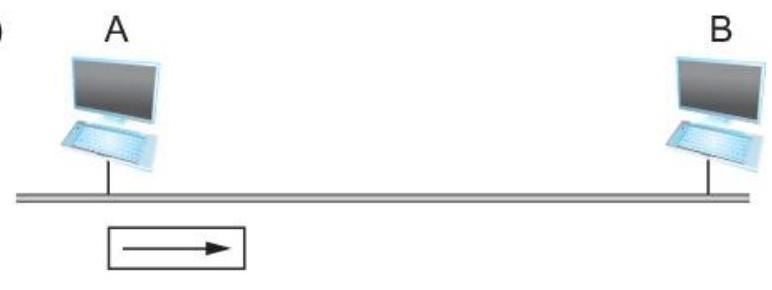
\includegraphics[max width=\textwidth]{2023_01_13_b07e3b4bcffdaab9792bg-121}
\end{center}

(b)

\begin{center}
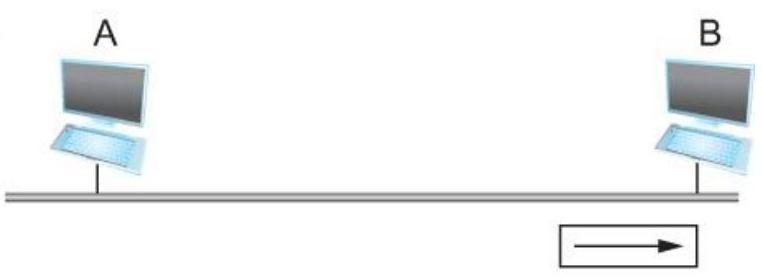
\includegraphics[max width=\textwidth]{2023_01_13_b07e3b4bcffdaab9792bg-121(1)}
\end{center}

(c)

\begin{center}
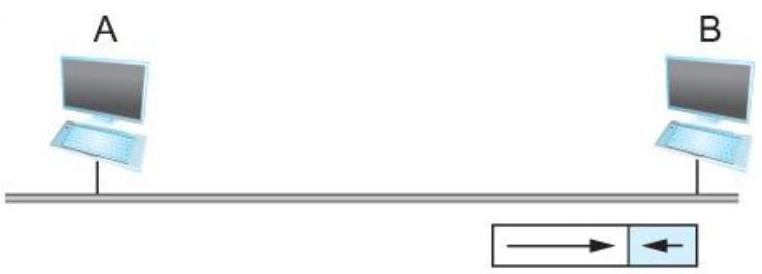
\includegraphics[max width=\textwidth]{2023_01_13_b07e3b4bcffdaab9792bg-121(2)}
\end{center}

(d) $\mathrm{A}$

\begin{center}
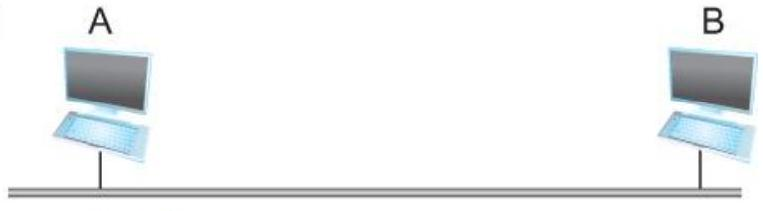
\includegraphics[max width=\textwidth]{2023_01_13_b07e3b4bcffdaab9792bg-121(3)}
\end{center}

Worst-case scenario:

(a) A sends a frame at time $t$;

(b) A's frame arrives at $\mathrm{B}$ at time $t+d$;

(c) B begins transmitting at time $t+d$ and collides with A's frame;

(d) B's runt (32-bit) frame arrives at $\mathrm{A}$ at time $t+2 d$.


\os{newpage} item[{\rot\bf  Ethernet Transmitter Algorithm }]~\\[-3ex]


\os{newpage} item[{\rot\bf  - Consider that a maximally configured Ethernet is 2500 $\mathrm{m}$ long, and there may be up to four repeaters between any two hosts, the round trip delay has been determined to be $51.2 \mu \mathrm{s }]~\\[-3ex]
$
 o Which on $10 \mathrm{Mbps}$ Ethernet corresponds to 512 bits}

\os{newpage} item[{\rot\bf  - The other way to look at this situation, }]~\\[-3ex]
\bi
 \ite We need to limit the Ethernet's maximum latency to a fairly small value $(51.2 \mu \mathrm{s})$ for the access algorithm to work
 \ei


\bi
  \ite Hence the maximum length for the Ethernet is on the order of $\mathbf{2 5 0 0}$ $\mathrm{m}$.
\ei


\os{newpage} item[{\rot\bf  Ethernet Transmitter Algorithm }]~\\[-3ex]

\bi
  \ite Once an adaptor has detected a collision, and stopped its transmission, it waits a certain amount of time and tries again.

  \ite Each time the adaptor tries to transmit but fails, it doubles the amount of time it waits before trying again.

  \ite This strategy of doubling the delay interval between each retransmission attempt is known as Exponential Backoff.

\ei


\os{newpage} item[{\rot\bf  Ethernet Transmitter Algorithm }]~\\[-3ex]

\bi
  \ite The adaptor first delays either o or $51.2 \mu \mathrm{s}$, selected at random.

  \ite If this effort fails, it then waits $0,51.2,102.4,153.6 \mu \mathrm{s}$ (selected randomly) before trying again;

  \ite This is $k^{*} 51.2$ for $k=0,1,2,3$

  \ite After the third collision, it waits $k^{*} 51.2$ for $k=0 \ldots 2^{3}-1$ (again selected at random).

  \ite In general, the algorithm randomly selects a $k$ between $o$ and $2^{\mathrm{n}}-1$ and waits for $k^{*} 51.2 \mu \mathrm{s}$, where $n$ is the number of collisions experienced so far.

\ei


\os{newpage} item[{\rot\bf  Experience with Ethernet }]~\\[-3ex]

\bi
  \ite Ethernets work best under lightly loaded conditions.

  \ite Under heavy loads, too much of the network's capacity is wasted by collisions.

  \ite Most Ethernets are used in a conservative way.

  \ite Have fewer than 200 hosts connected to them which is far fewer than the maximum of 1024.

  \ite Most Ethernets are far shorter than $2500 m$ with a round-trip delay of closer to $5 \mu$ s than $51.2 \mu \mathrm{s}$.

  \ite Ethernets are easy to administer and maintain.

  \ite There are no switches that can fail and no routing and configuration tables that have to be kept up-to-date.

  \ite It is easy to add a new host to the network.

  \ite It is inexpensive.

\ei

C Cable is cheap, and only other cost is the network adaptor on each host.


\os{newpage} item[{\rot\bf  Orientation }]~\\[-3ex]

1

2

\bi
  \ite IP (Internet Protocol) is a Network Layer Protocol.
\ei

\begin{center}
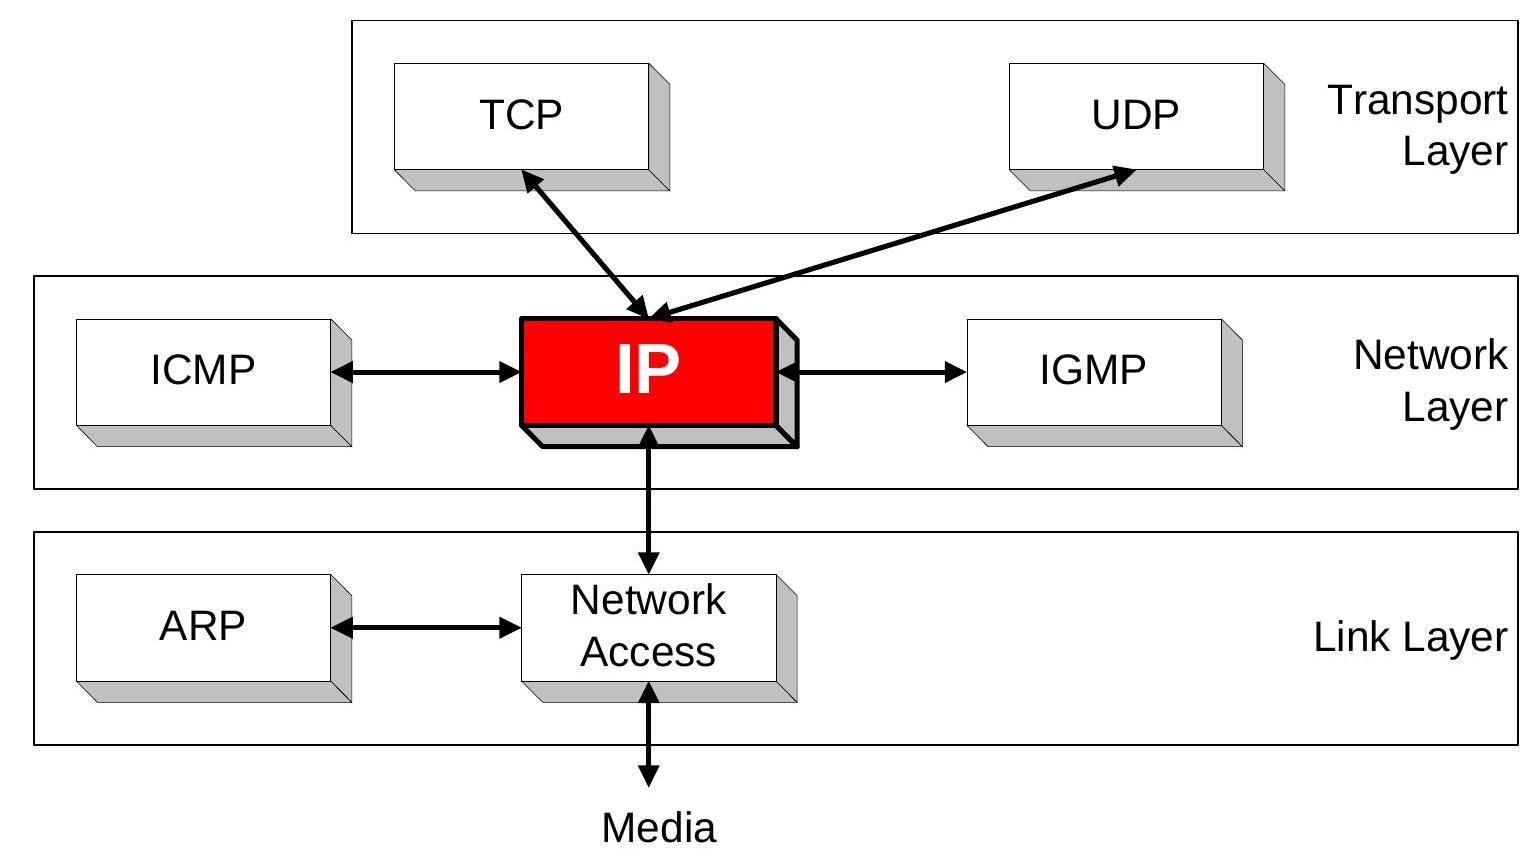
\includegraphics[max width=\textwidth]{2023_01_13_b07e3b4bcffdaab9792bg-127}
\end{center}

\bi
  \ite IP's current version is Version 4 (IPv4). It is specified in RFC 891.
\ei


\os{newpage} item[{\rot\bf  IP: The waist of the hourglass }]~\\[-3ex]

1

2

\bi
  \ite IP is the waist of the liourglass of the Internet protocol architecture

  \ite Multiple higher-layer protocols

  \ite Multiple lower-layer protocols

  \ite Only one protocol at the network

\ei

\begin{center}
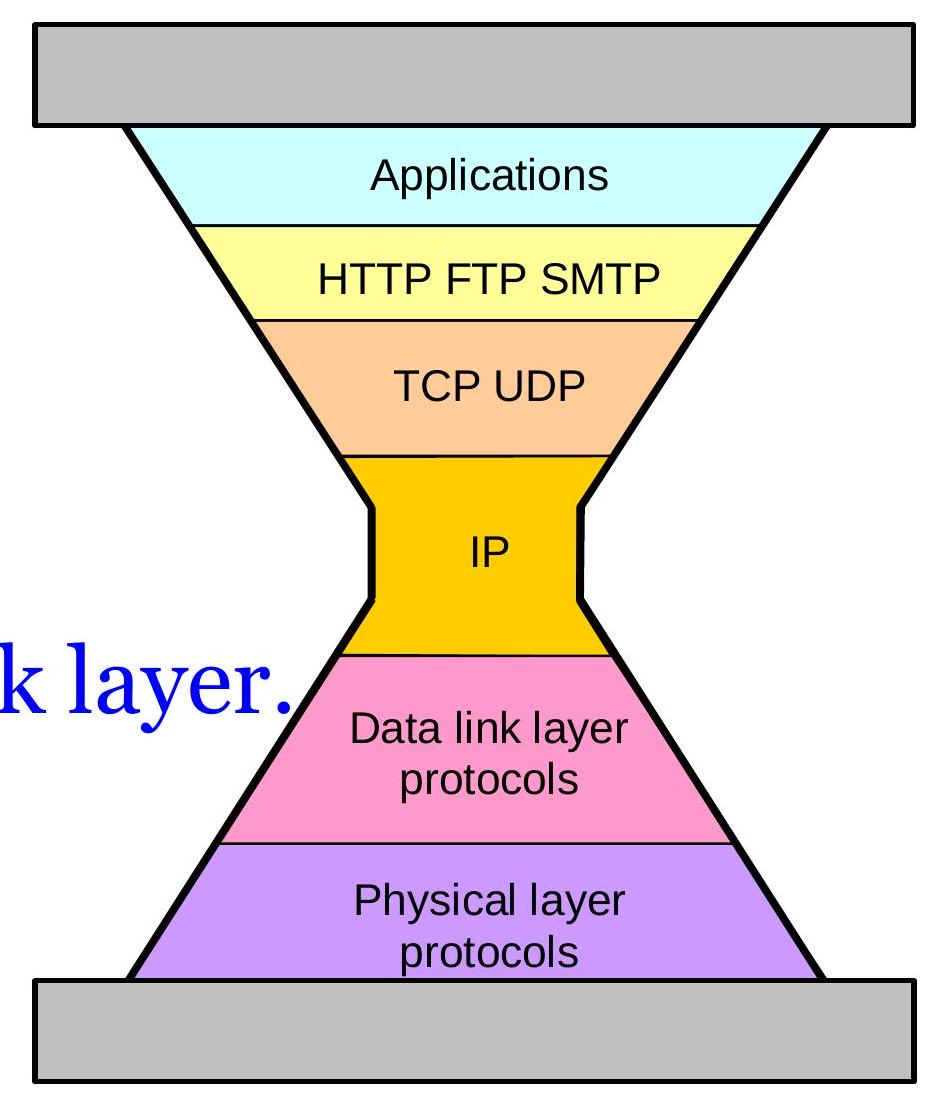
\includegraphics[max width=\textwidth]{2023_01_13_b07e3b4bcffdaab9792bg-128}
\end{center}


\os{newpage} item[{\rot\bf  Application protocol }]~\\[-3ex]

1

2

\bi
  \ite IP is the highest layer protocol which is implemented at both routers and hosts
\ei

\begin{center}
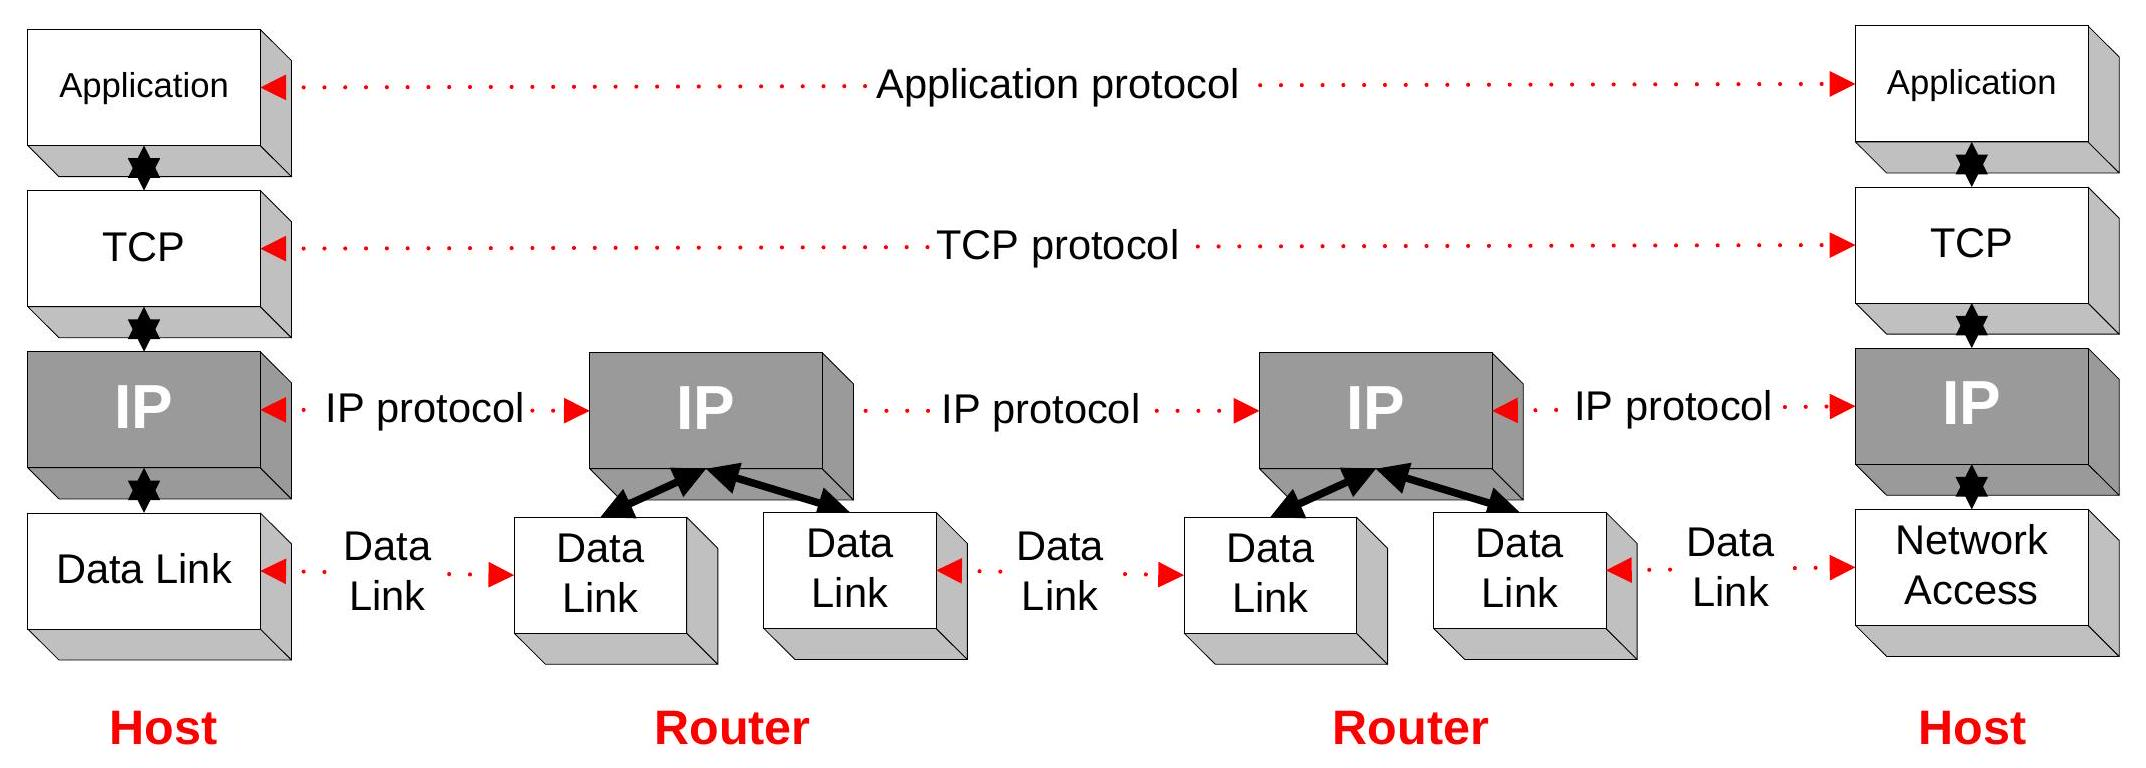
\includegraphics[max width=\textwidth]{2023_01_13_b07e3b4bcffdaab9792bg-129}
\end{center}


\os{newpage} item[{\rot\bf  IP Service }]~\\[-3ex]

\bi
  \ite Delivery service of IP is minimal 1
3
0

  \ite IP provide provides an unreliable connectionless best effort service (also called: "datagram service").

\ei
\bi
 \ite Unreliable: IP does not make an attempt to recover lost packets
 \ei

\bi
 \ite Connectionless: Each packet ("datagram") is handled independently. IP is not aware that packets between hosts may be sent in a logical sequence
 \ei

\bi
 \ite Best effort: IP does not make guarantees on the service (no throughput guarantee, no delay guarantee,..)
 \ei



\os{newpage} item[{\rot\bf  - Consequences: }]~\\[-3ex]

\bi
  \ite Higher layer protocols have to deal with losses or with duplicate packets

  \ite Packets may be delivered out-of-sequence

\ei


\os{newpage} item[{\rot\bf  IP Service }]~\\[-3ex]

1

3

\bi
  \ite IP supports the following services:
\ei

ane-to-one

cone-to-all

rone-to-several

\begin{center}
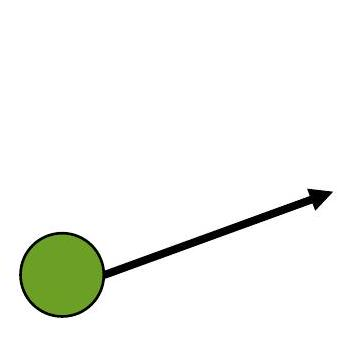
\includegraphics[max width=\textwidth]{2023_01_13_b07e3b4bcffdaab9792bg-131}
\end{center}

unicast

\begin{center}
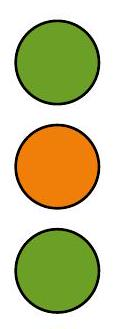
\includegraphics[max width=\textwidth]{2023_01_13_b07e3b4bcffdaab9792bg-131(1)}
\end{center}

broadcast (unicast)

(broadcast)

(multicast)

\begin{center}
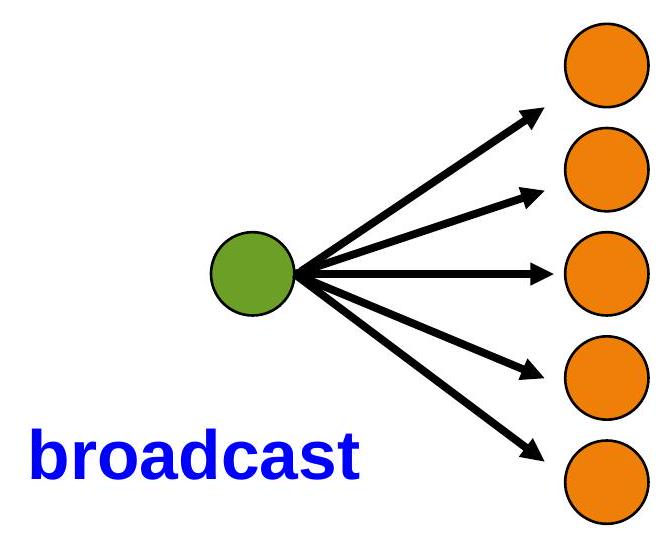
\includegraphics[max width=\textwidth]{2023_01_13_b07e3b4bcffdaab9792bg-131(2)}
\end{center}

\begin{center}
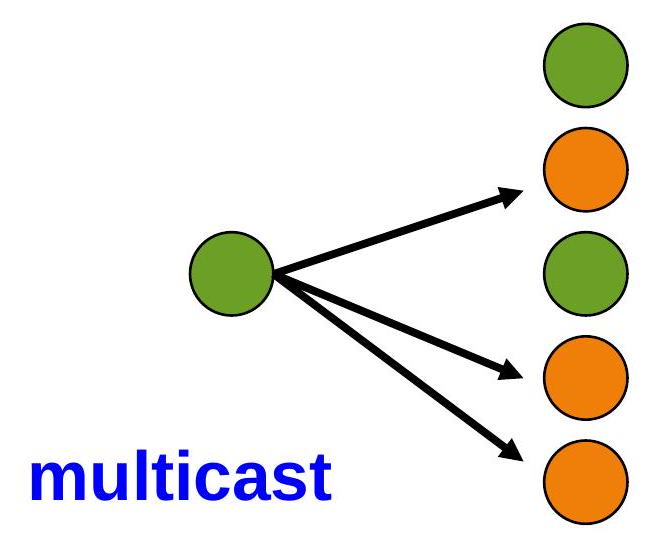
\includegraphics[max width=\textwidth]{2023_01_13_b07e3b4bcffdaab9792bg-131(3)}
\end{center}

\bi
  \ite IP multicast also supports a many-to-many service.

  \ite IP multicast requires support of other protocols (IGMP, multicast routing)

\ei

\os{newpage} item[{\rot\bf IP Datagram Format }]~\\[-3ex]


\bi
  \ite 20 bytes $\leq$ Header Size $<2^{4}$ x 4 bytes $=60$ bytes

  \ite 20 bytes $\leq$ Total Length $<2^{16}$ bytes $=65536$ bytes

\ei

\begin{center}
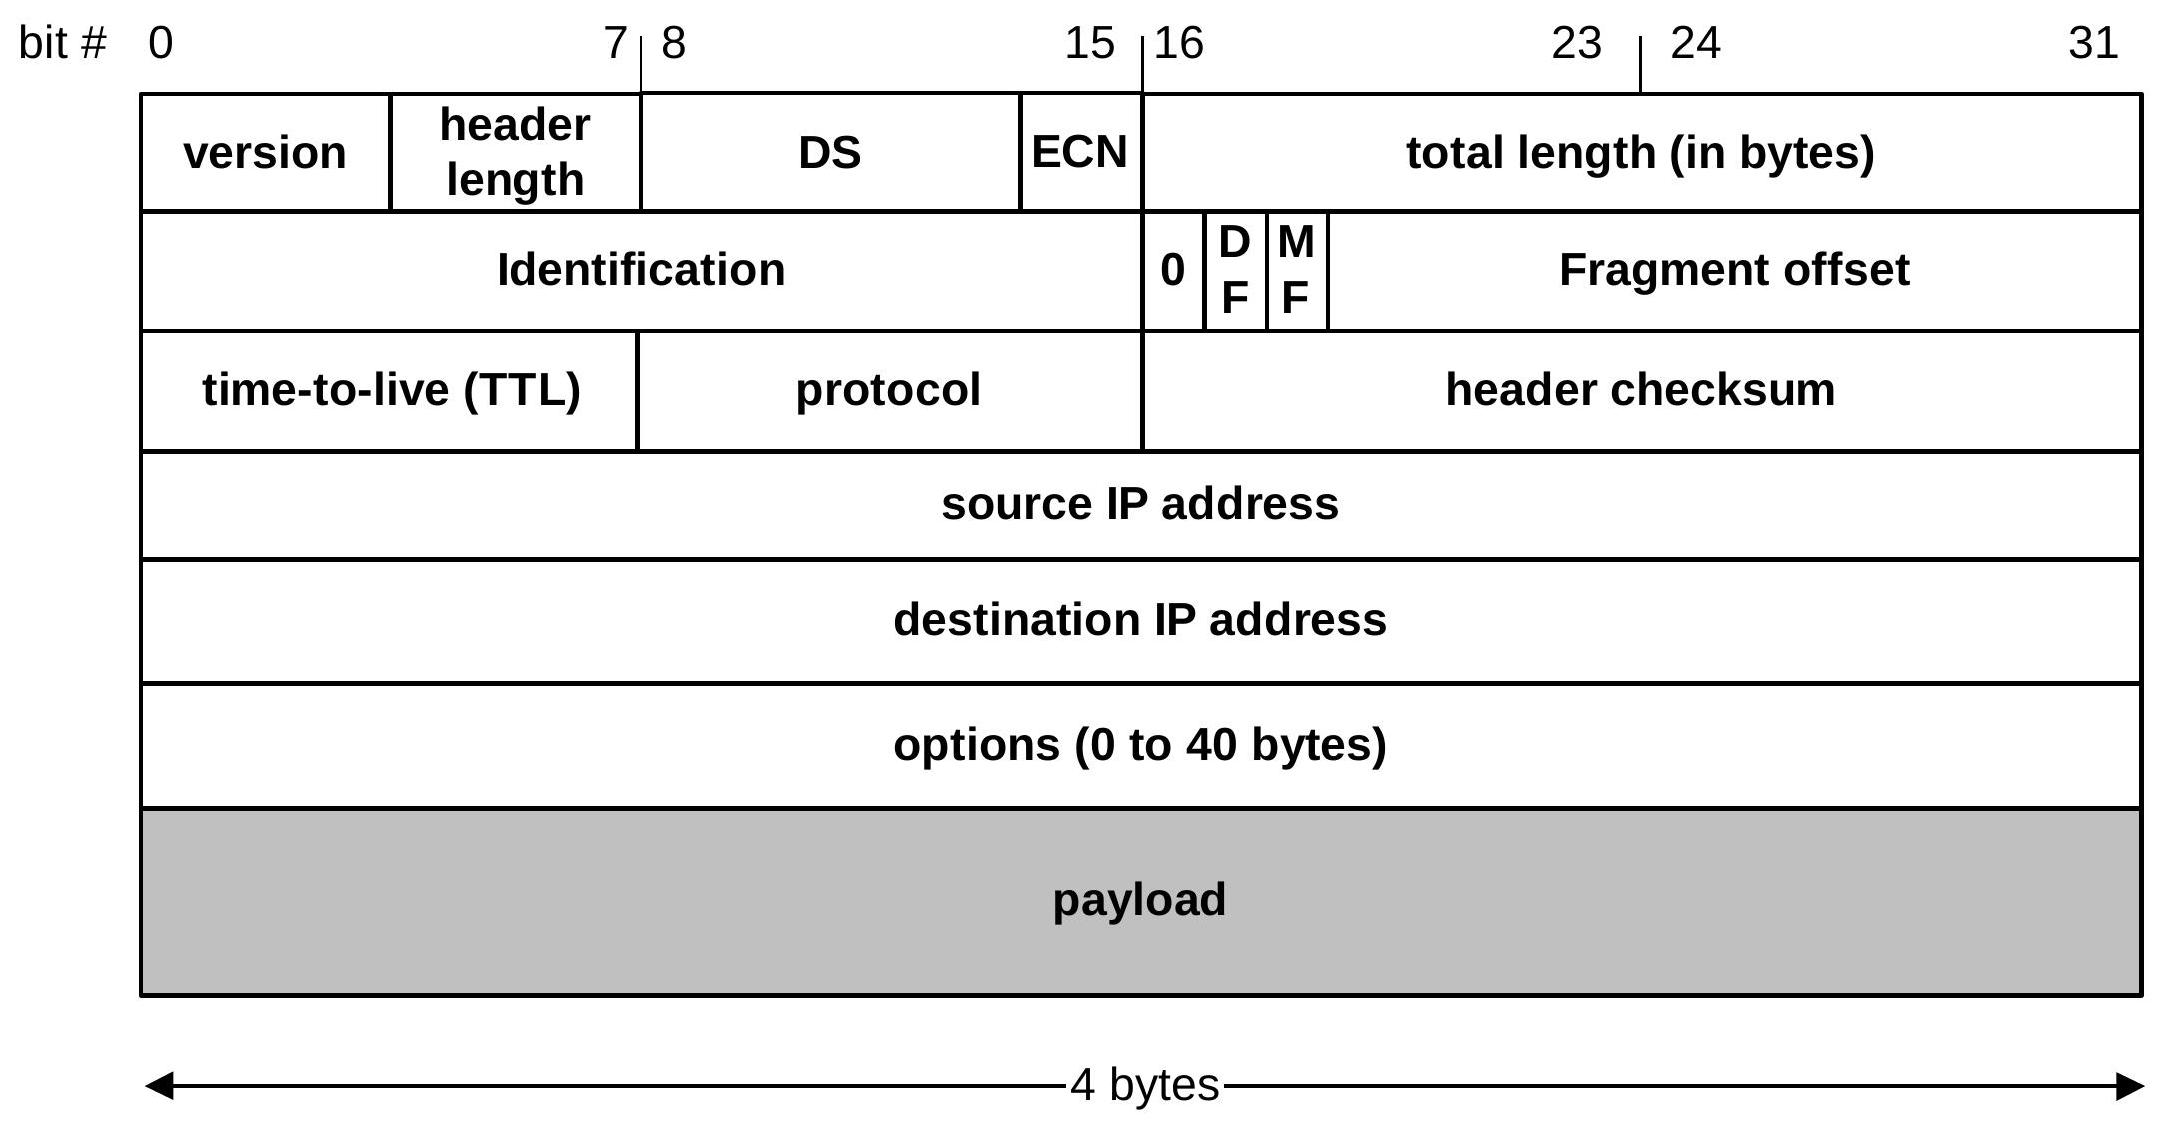
\includegraphics[max width=\textwidth]{2023_01_13_b07e3b4bcffdaab9792bg-132}
\end{center}


\os{newpage} item[{\rot\bf  IP Datagram Format }]~\\[-3ex]

$$
1
$$

3

\bi
  \ite Question: In which order are the bytes of an IP datagram transmitted?

  \ite Answer:

  \ite Transmission is row by row

  \ite For each row:

\ei

\begin{enumerate}
  \ite First transmit bits $0-7$

  \ite Then transmit bits $8-15$

  \ite Then transmit bits 16-23

  \ite Then transmit bits 24-31

\end{enumerate}


\os{newpage} item[{\rot\bf  - This is called network byte order or big endian byte ordering. }]~\\[-3ex]

\bi
  \ite Note: Many computers (incl. Intel processors) store 32-bit words in little endian format. Others (incl. Motorola processors) use big endian.
\ei


\os{newpage} item[{\rot\bf  Big endian vs. small endian }]~\\[-3ex]


\bi
  \ite Conventions to store a multibyte work

  \ite Example: a 4 byte Long Integer Byte3 Byte2 Byte1 Byte0

\ei


\os{newpage} item[{\rot\bf  Little Endian }]~\\[-3ex]

\bi
  \ite Stores the low-order byte at the lowest address and the highest order byte in the highest address.
\ei

Base Addresst0 Byte0 Base Addresst1 Byte1 Base Address+2 Byte2 Base Address+3 Byte3

\bi
  \ite Intel processors use this order
\ei


\os{newpage} item[{\rot\bf  Big Endian }]~\\[-3ex]

\bi
  \ite Stores the high-order byte at the lowest address, and the low-order byte at the highest address.
Base Address+0 Byte3
Base Addresst1 Byte2
Base Addresst2 Byte1
Base Address+3 Byte0
\ei

Motorola processors use big endian.

\os{newpage} item[{\rot\bf Fields of the IP Header } ]~\\[-3ex]


\bi
  \ite Version (4 bits): current version is 4, next version will be 6.

  \ite Header length (4 bits): length of IP header, in multiples of 4 bytes

  \ite DS/ECN field (1 byte)

\ei
\bi
 \ite This field was previously called as Type-of-Service (TOS) field. The role of this field has been re-defined, but is "backwards compatible" to TOS interpretation
 \ei

\bi
 \ite Differentiated Service (DS) (6 bits):
 \ei


\bi
  \ite Used to specify service level (currently not supported in the Internet)
\ei
\bi
 \ite Explicit Congestion Notification (ECN) (2 bits):
 \ei


\begin{CJK}{UTF8}{mj}乂\end{CJK} New feedback mechanism used by TCP

\os{newpage} item[{\rot\bf Fields of the IP Header } ]~\\[-3ex]


\bi
  \ite Identification (16 bits): Unique identification of a datagram from a host. Incremented whenever a datagram is transmitted

  \ite Flags (3 bits):

  \ite First bit always set to 0

\ei
\bi
 \ite DF bit (Do not fragment)
 \ei

\bi
 \ite MF bit (More fragments)
 \ei


Will be explained later $\rightarrow$ Fragmentation


\os{newpage} item[{\rot\bf  Fields of the IP Header }]~\\[-3ex]

1

3

\bi
  \ite Time To Live (TTL) (17byte):
\ei
\bi
 \ite Specifies longest paths before datagram is dropped
 \ei

\bi
 \ite Role of TTL field: Ensure that packet is eventually dropped when a routing loop occurs
 \ei


Used as follows:
\bi
 \ite Sender sets the value (e.g., 64)
 \ei

\bi
 \ite Each router decrements the value by 1
 \ei

\bi
 \ite When the value reaches 0 , the datagram is dropped
 \ei



\os{newpage} item[{\rot\bf  Fields of the IP Header }]~\\[-3ex]

1

\bi
  \ite Protocol (1 byte):
\ei

3

8

\bi
  \ite Specifies the higher-layer protocol.
\ei

\bi
  \ite Used for demultiplexing to higher layers.
\ei

\begin{center}
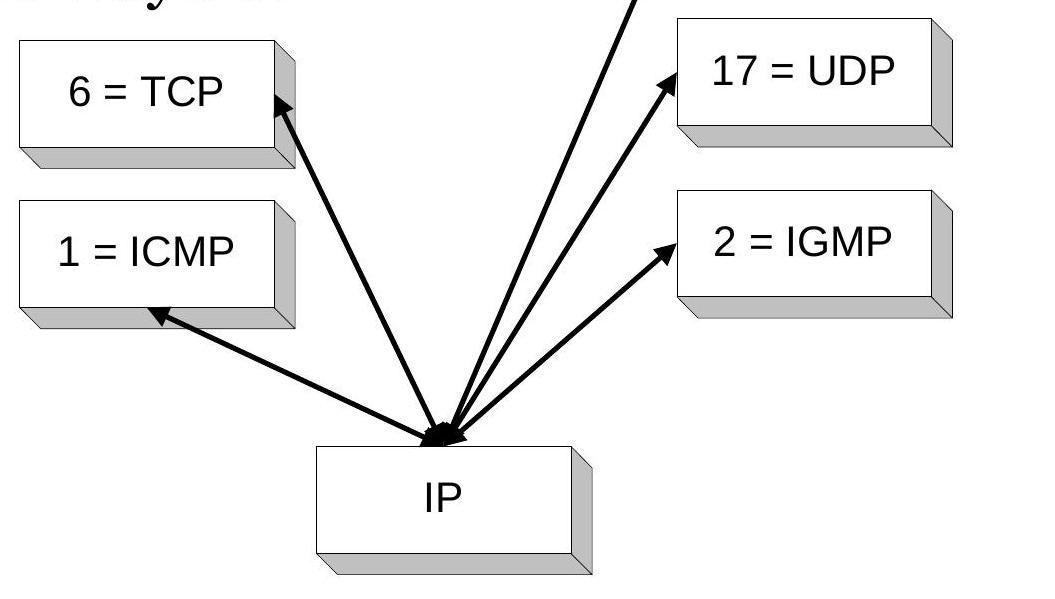
\includegraphics[max width=\textwidth]{2023_01_13_b07e3b4bcffdaab9792bg-138}
\end{center}

\bi
  \ite Header checksum (2 bytes): A simple 16-bit long checksum which is computed for the header of the datagram.
\ei

\os{newpage} item[{\rot\bf   Fields of the IP Header } ]~\\[-3ex]



\os{newpage} item[{\rot\bf  - Options: }]~\\[-3ex]

9

\bi
  \ite Security restrictions
\ei

Record Route: each router that processes the packet adds its IP address to the header.

Timestamp: each router that processes the packet adds its IP address and time to the header.

(loose) Source Routing: specifies a list of routers that must be traversed.

\bi
  \ite (strict) Source Routing: specifies a list of the only routers that can be traversed.
\ei


\os{newpage} item[{\rot\bf  - Padding: Padding bytes are added to ensure that header ends on a 4-byte boundary }]~\\[-3ex]


\os{newpage} item[{\rot\bf  Maximum Transmission Unit }]~\\[-3ex]

1

4

\bi
  \ite Maximum size of IP datagram is 65535 , but the data link layer protocol generally imposes a limit that is much smaller

  \ite Example:

\ei
\bi
 \ite Ethernet frames have a maximum payload of 1500 bytes
 \ei


$\rightarrow$ IP datagrams encapsulated in Ethernet frame cannot be longer than 1500 bytes

\bi
  \ite The limit on the maximum IP datagram size, imposed by the data link protocol is called maximum transmission unit (MTU)

  \ite MTUs for various data link protocols:

\ei

Ethernet: $\quad 1500$

802.3:

802.5: 1492

4464 FDDI: $\quad 4352$

ATM AAL5: 9180

PPP:


\item[{\rot\bf  IP Fragmentation  }]~\\[-3ex]
 ]~\\[-3ex]


\bi
  \ite What if the size of an IP datagram exceeds the MTU? IP datagram is fragmented into smaller units.

  \ite What if the route contains networks with different MTUs?

\ei

\begin{center}
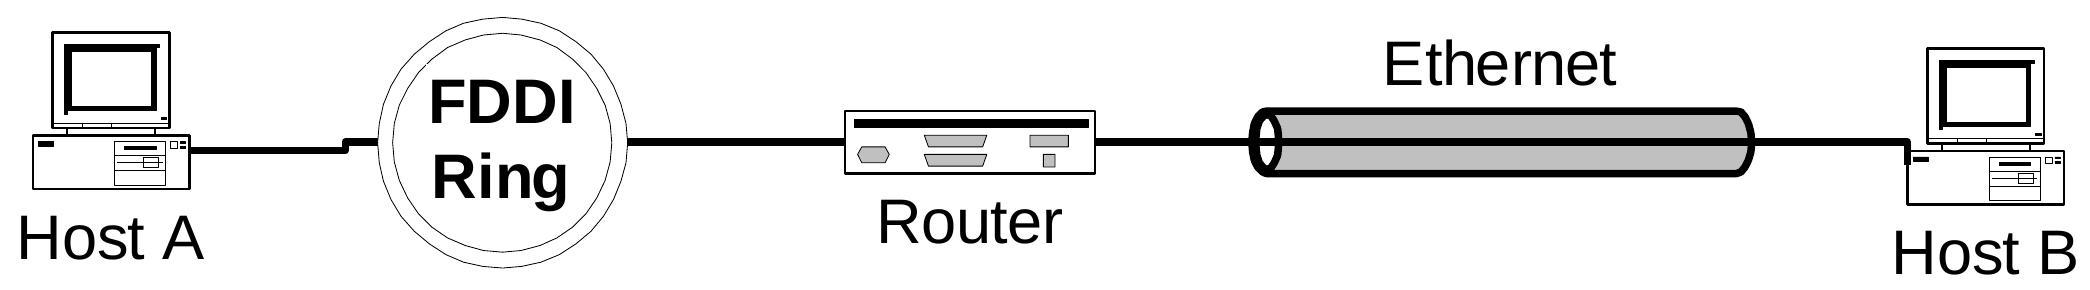
\includegraphics[max width=\textwidth]{2023_01_13_b07e3b4bcffdaab9792bg-141}
\end{center}

MTUs: FDDI: 4352

Ethernet: 1500

\bi
  \ite Fragmentation:

  \ite IP router splits the datagram into several datagram

  \ite Fragments are reassembled at receiver

\ei


\item[{\rot\bf  Where is Fragmentation done?  }]~\\[-3ex]



\bi
  \ite Fragmentation can be done at the sender or at intermediate routers
\ei

×he same datagram can be fragmented several times.

 Reassembly of original datagram is only done at destination hosts !!
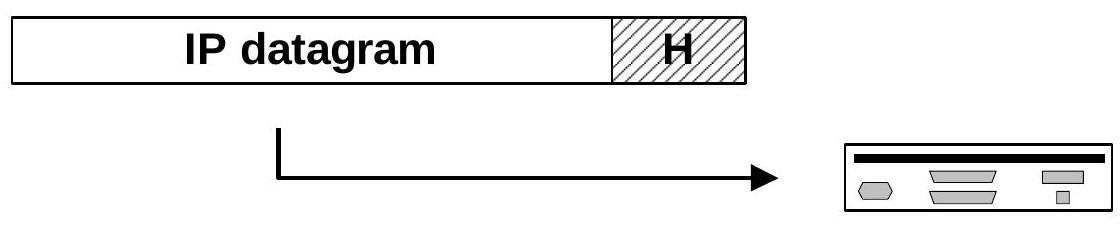
\includegraphics[max width=\textwidth, center]{2023_01_13_b07e3b4bcffdaab9792bg-142}

Fragment 2

42

Fragment 1

(1)

Router


\os{newpage} item[{\rot\bf  What's involved in Fragmentation? }]~\\[-3ex]

\bi
  \ite The following fields in the IP header are involved:
\ei

\begin{center}
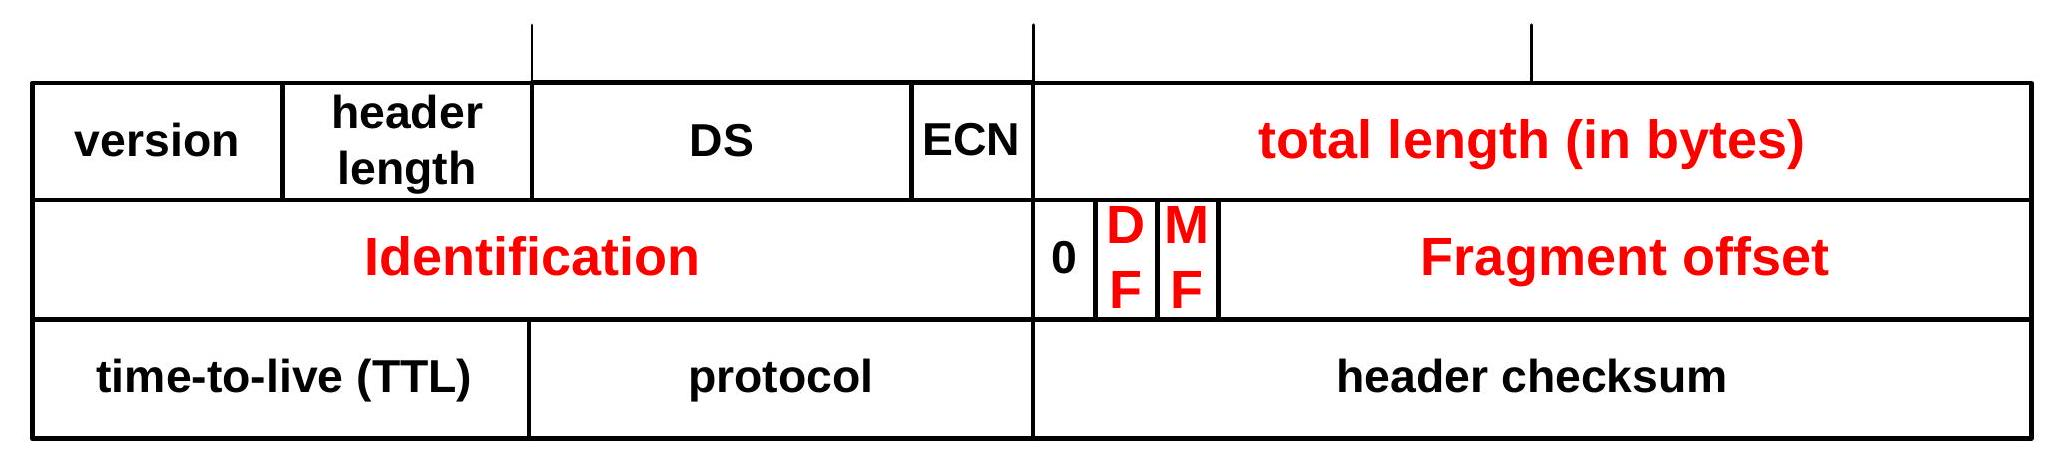
\includegraphics[max width=\textwidth]{2023_01_13_b07e3b4bcffdaab9792bg-143}
\end{center}

Identification

Flags When a datagram is fragmented, the identification is the same in all fragments

DF bit is set: Datagram cannot be fragmented and must be discarded if MTU is too small

MF bit set: This datagram is part of a fragment and an additional fragment follows this one


\os{newpage} item[{\rot\bf  What's involved in Fragmentation? }]~\\[-3ex]

\bi
  \ite The following fields in the IP header are involved:
\ei

\begin{center}
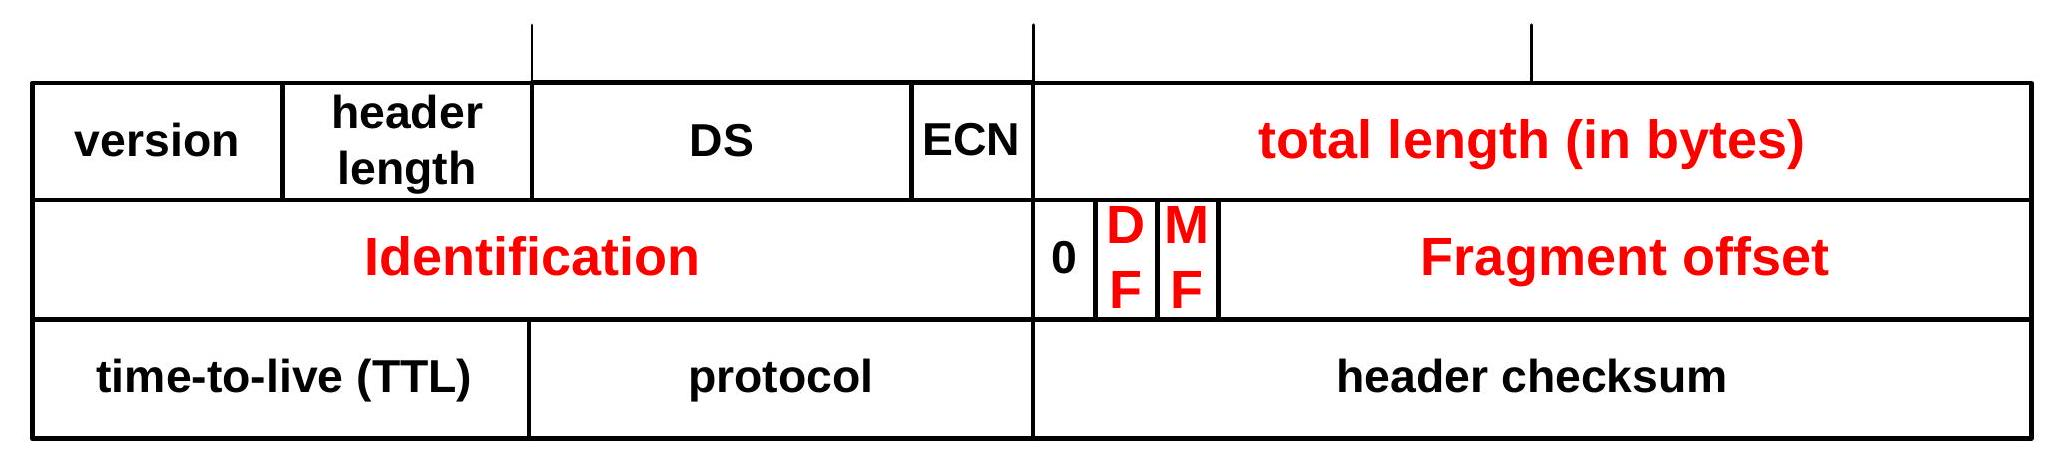
\includegraphics[max width=\textwidth]{2023_01_13_b07e3b4bcffdaab9792bg-144}
\end{center}

Fragment offset Offset of the payload of the current fragment in the original datagram Total length

Total length of the current fragment


\item[{\rot\bf  Example of Fragmentation  }]~\\[-3ex]



\bi
  \ite A datagram with size 2400 bytes isust be fragmented according to an MTU limit of 1000 bytes
\ei

Header length: 20 Total length: 2400 Identification: 0xa428

DF flag: 0 MF flag: 0

Fragment offset: 0 Header length: 20

Total length: 448 Identification: 0xa428

DF flag: 0

MF flag: 0

Fragment offset: 244 Header length: 20

Total length: 996 Identification: 0xa428 DF flag: 0 MF flag: 1 Fragment offset: 122 Header length: 20 Total length: 996 Identification: 0xa428 DF flag: 0 MF flag: 1 fragment offset: 0
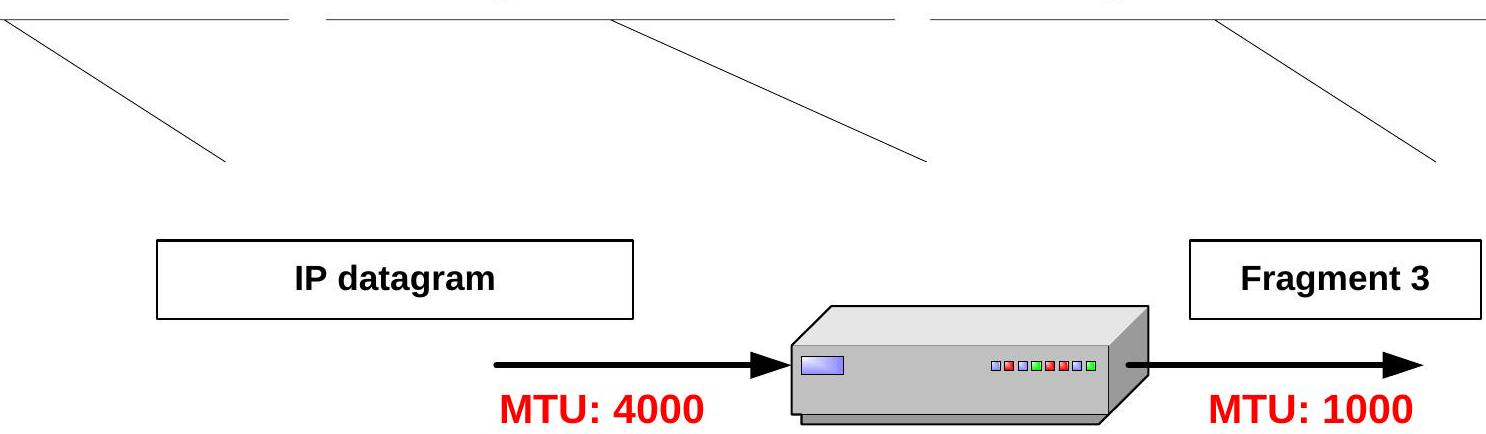
\includegraphics[max width=\textwidth, center]{2023_01_13_b07e3b4bcffdaab9792bg-145}

Fragment 2

Fragment 1

Router


\os{newpage} item[{\rot\bf  Determining the length of fragments }]~\\[-3ex]

1

4

\bi
  \ite To determine the size of the fragments we recall that, since there are only 13 bits available for the fragment offset, the offset is given as a multiple of eight bytes.

  \ite a result, the first and second fragment have a size of 996 bytes (and not 1000 bytes). This number is chosen since 976 is the largest number smaller than $1000-20=980$ that is divisible by eight.

  \ite The payload for the first and second fragments is 976 bytes long, with bytes o through 975 of the original IP payload in the first fragment, and bytes 976 through 1951 in the second fragment.

  \ite The payload of the third fragment has the remaining 428 bytes, from byte 1952 through 2379.

  \ite With these considerations, we can determine the values of the fragment offset, which are $0,976 / 8=122$, and $1952 / 8=$ 244 , respectively, for the first, second and third fragment.

\ei


\os{newpage} item[{\rot\bf  IP Addressing }]~\\[-3ex]


\item[{\rot\bf  What is an IP address?  }]~\\[-3ex]


\os{newpage} item[{\rot\bf  - An unique identifier for a computer or device (host) on a TCP/IP network }]~\\[-3ex]


\os{newpage} item[{\rot\bf  - A 32-bit binary number usually represented as 4 decimal numbers separated by a period }]~\\[-3ex]




\item[{\rot\bf  What is an IP address?  }]~\\[-3ex]


\os{newpage} item[{\rot\bf  - Each address is $3^{2}$ bits wide }]~\\[-3ex]

\bi
  \ite Valid addresses can range from 0.0.0.0 to 255.255.255.255
\ei




\item[{\rot\bf  What is an IP address?  }]~\\[-3ex]


\os{newpage} item[{\rot\bf  Theoretically, a total of $\approx 4.3$ billion addresses are available }]~\\[-3ex]




\os{newpage} item[{\rot\bf  Two addresses in one... }]~\\[-3ex]


\os{newpage} item[{\rot\bf  Each address consists of two parts }]~\\[-3ex]


\os{newpage} item[{\rot\bf  The network address }]~\\[-3ex]


\os{newpage} item[{\rot\bf  The host address }]~\\[-3ex]


\os{newpage} item[{\rot\bf  Other systems may use more than one address (Ex: IPX) }]~\\[-3ex]


\os{newpage} item[{\rot\bf  The Five Network Classes }]~\\[-3ex]

\begin{enumerate}
  \ite Class $\mathrm{A}-$ begins with 0
\end{enumerate}

\bi
  \ite $00000001\left(1_{10}\right)$ to $01111111\left(126_{10}\right)^{*}$
\ei

\begin{enumerate}
  \setcounter{enumi}{1}
  \ite Class $\mathbf{B}-$ begins with $\mathbf{1 0}$
\end{enumerate}

\bi
  \ite $10000000\left(128_{10}\right)$ to $10111111\left(191_{10}\right)$
\ei


\os{newpage} item[{\rot\bf  Class $\mathrm{C}-$ begins with $\mathbf{1 1 0}$ }]~\\[-3ex]

\bi
  \ite $11000000\left(192_{10}\right)$ to $11011111\left(223_{10}\right)$
\ei

$* 01111111=127_{10}$


\os{newpage} item[{\rot\bf  Addresses beginning with 127 are reserved for loopback (127.0.0.1 is YoU) }]~\\[-3ex]


\os{newpage} item[{\rot\bf  The Five Network Classes }]~\\[-3ex]


\os{newpage} item[{\rot\bf  Class $\mathrm{D}$ - begins with 1110 }]~\\[-3ex]

\bi
  \ite $224_{10}$ to $239_{10}$

  \ite Reserved for multicasting

\ei


\os{newpage} item[{\rot\bf  Class E - begins with $\mathbf{1 1 1 1}$ }]~\\[-3ex]

\bi
  \ite $240_{10}$ to $254_{10}$

  \ite Reserved for future use

\ei


\os{newpage} item[{\rot\bf  These should not be used for host addressing }]~\\[-3ex]


\item[{\rot\bf  Which part belongs to the network and which part belongs to the node?  }]~\\[-3ex]



\os{newpage} item[{\rot\bf  Class B - XXXXXXXX.XXXXXXXX.yyyyyyyy.yyyyyyyy }]~\\[-3ex]


\os{newpage} item[{\rot\bf  Class C - XXXXXXXX.XXXXXXXX.XXXXXXXX.yyyyyyyy }]~\\[-3ex]


\os{newpage} item[{\rot\bf  Where $X=$ Network and $y=$ node }]~\\[-3ex]


\os{newpage} item[{\rot\bf  IP Addresses* }]~\\[-3ex]


\os{newpage} item[{\rot\bf  Class $1^{\text {st }}$ Octet Networks Ids Host IDs }]~\\[-3ex]

\begin{center}
\begin{tabular}{|c|c|c|c|}
\hline
$A$ & $1-126$ & $2^{7}=126$ & $2^{24}=16 M$ \\
\hline
$B$ & $128-191$ & $2^{14}=16 K$ & $2^{16}=64 K$ \\
\hline
$C$ & $192-223$ & $2^{21}=2 M$ & $2^{8}=255$ \\
\hline
\end{tabular}
\end{center}


\os{newpage} item[{\rot\bf  There are three IP network addresses reserved for private networks }]~\\[-3ex]

\begin{enumerate}
  \ite $10.0 .0 .0 / 8$

  \ite $172.16 .0 .0 / 12$

  \ite $192.168 .0 .0 / 16$

\end{enumerate}


\os{newpage} item[{\rot\bf  These can be used by anyone setting up an internal network. }]~\\[-3ex]


\os{newpage} item[{\rot\bf  Routers will never forward packets coming from these addresses. }]~\\[-3ex]


\os{newpage} item[{\rot\bf  Subnetting }]~\\[-3ex]

...can be done for a variety of reasons
\bi
 \ite Organization
 \ei


\bi
  \ite Use of different physical media

  \ite Preservation of address space

\ei
\bi
 \ite Security
 \ei


\bi
  \ite The most common reason is to control network traffic
\ei


\os{newpage} item[{\rot\bf  Subnetting }]~\\[-3ex]

\bi
  \ite In an Ethernet network, all nodes on a segment see all packets transmitted by other nodes on that segment

  \ite Performance can be adversely affected under heavy traffic loads

  \ite A router is used to connect IP networks to minimize the amount of traffic each segment must receive

\ei


\os{newpage} item[{\rot\bf  Subnet masking }]~\\[-3ex]

\bi
  \ite Applying a subnet mask allows you to identify the network and node parts of the address. A router will then determine whether the address is local or remote.

  \ite Network bits are masked as 1s

  \ite Node bits are masked as os

  \ite Class A - 255.0.0.0

\ei
\bi
 \ite 11111111.00000000.00000000.00000000
 \ei


\bi
  \ite Class B - 255.255.0.0
\ei

O 11111111.11111111.00000000.00000000

\bi
  \ite Class C - 255.255.255.0
\ei
\bi
 \ite 11111111.11111111.11111111.00000000
 \ei



\os{newpage} item[{\rot\bf  Subnet masking }]~\\[-3ex]

cil c: WINDOWS system32 cmd.exe

$P: \backslash>$ ipconfig $/ \mathbf{a l l}$

Windows IP Conf iguration

Host Name : - $-\cdot \cdot \cdot \cdot \cdot \cdot \cdot \cdot \cdot \cdot=$ D201B-01

\begin{center}
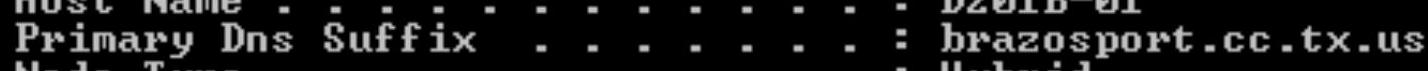
\includegraphics[max width=\textwidth]{2023_01_13_b07e3b4bcffdaab9792bg-160}
\end{center}

Node Type ... . . . . . . . . Hybrid

IP Routing Enabled: : : : : : : No

WINS Proxy Enabled.: :.:-:.: No

DNS Suffix Search List... . . : \href{http://Hrazosport.cc.tx.us}{Hrazosport.cc.tx.us}

\href{http://cc.tx.us}{cc.tx.us}

\href{http://tx.us}{tx.us}

Ethernet adapter Local Area Connection:

Connection-specific DNS Suffix

\begin{center}
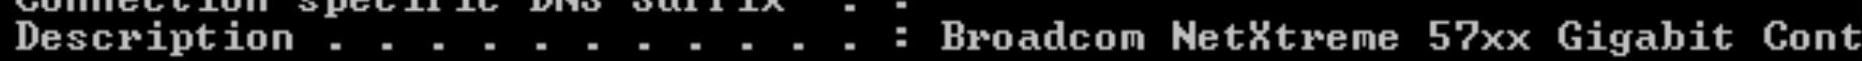
\includegraphics[max width=\textwidth]{2023_01_13_b07e3b4bcffdaab9792bg-160(1)}
\end{center}

rollers

Physical Address . . . . . . . . . : 00-19-B9-46-38-F2

Dhcp Enabled. . . . . . . . . . . : No

\begin{center}

\includegraphics[max width=\textwidth]{2023_01_13_b07e3b4bcffdaab9792bg-160(2)}
\end{center}

\begin{center}

\includegraphics[max width=\textwidth]{2023_01_13_b07e3b4bcffdaab9792bg-160(3)}
\end{center}

\begin{center}

\includegraphics[max width=\textwidth]{2023_01_13_b07e3b4bcffdaab9792bg-160(4)}
\end{center}

DNS Seruers. $=.-.=.-.=-206.40 .177 .10$

$206.40 .177 .11$

$P: \backslash>$


\os{newpage} item[{\rot\bf  Subnet masking }]~\\[-3ex]

\bi
  \ite Performing a bitwise logical AND between the IP address and the subnet mask results in the network address

  \ite Ex: Class - B 140.179.240.200

\ei

10001100.10110011.11110000.11001000

11111111.11111111.00000000.00000000

10001100.10110011.00000000.00000000

Network Address $=140.179 .000 .000$


\item[{\rot\bf  A Few Rules...  }]~\\[-3ex]


\os{newpage} item[{\rot\bf  Each device on a node has a unique MAC address }]~\\[-3ex]


\os{newpage} item[{\rot\bf  Each device on a node needs a unique IP address }]~\\[-3ex]


\os{newpage} item[{\rot\bf  All devices on the same physical segment share a common network ID (subnet mask) }]~\\[-3ex]




\os{newpage} item[{\rot\bf  Address Resolution Protocol (ARP) }]~\\[-3ex]

\bi
  \ite Before an IP packet can be forwarded to another host, the MAC address (usually 6 bytes written in hex (Ex: 02-FE-874A-8C-A9) of the receiving machine must be known

  \ite ARP determines the MAC addresses that correspond to an IP address

  \ite A router will choose direct paths for the network packets based on the addressing of the IP frame it is handling (different routes to different networks)

\ei


\os{newpage} item[{\rot\bf  Address Resolution Protocol (ARP) }]~\\[-3ex]


\item[{\rot\bf  Internet and Data Link Layer Addresses  }]~\\[-3ex]

\bi
  \ite Each host and router on a subnet needs a data link layer address to specify its address on the subnet
\ei

\begin{center}
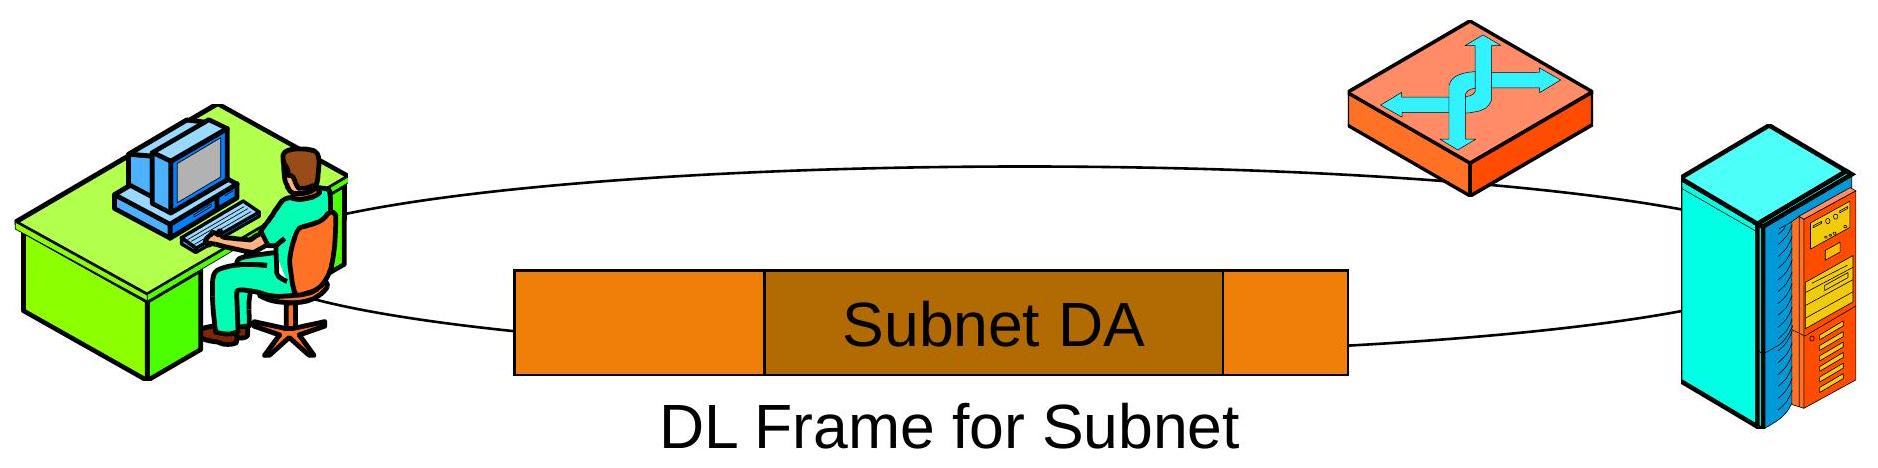
\includegraphics[max width=\textwidth]{2023_01_13_b07e3b4bcffdaab9792bg-165}
\end{center}


\os{newpage} item[{\rot\bf  Addresses }]~\\[-3ex]

\bi
  \ite Each host and router also needs an IP address at the internet layer to designate its position in the overall Internet
\ei

\begin{center}
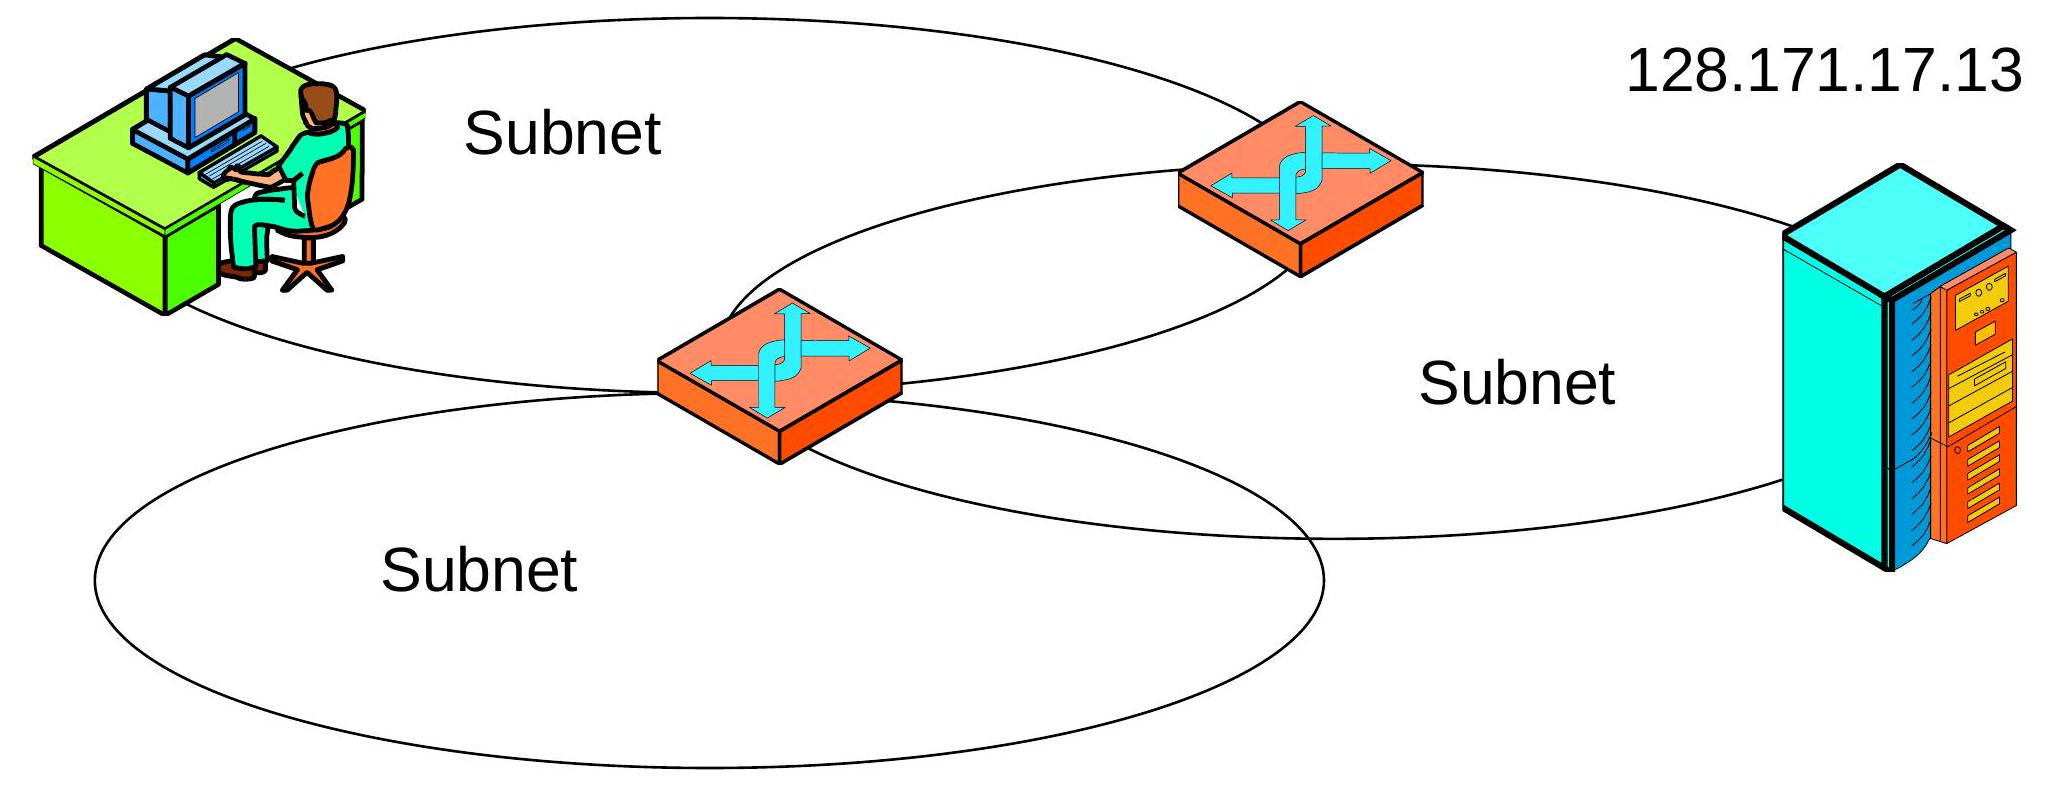
\includegraphics[max width=\textwidth]{2023_01_13_b07e3b4bcffdaab9792bg-166}
\end{center}


\os{newpage} item[{\rot\bf  Internet and Data Link Addresses Serve Different Purposes }]~\\[-3ex]

\begin{center}

\includegraphics[max width=\textwidth]{2023_01_13_b07e3b4bcffdaab9792bg-167}
\end{center}

\bi
  \ite IP address
\ei
\bi
 \ite To guide delivery to destination host across the Internet (across multiple networks)
 \ei


\bi
  \ite Subnet Address
\ei
\bi
 \ite To guide delivery between two hosts, two routers, and a host and router within a single subnet
 \ei


\bi
  \ite Same LAN, Frame Relay network, etc.
\ei


\os{newpage} item[{\rot\bf  Analogy }]~\\[-3ex]

\bi
  \ite In company, each person has a company-wide ID number (like IP address)

  \ite In company, person also has a local office number in a building

  \ite Paychecks are made out to ID numbers

  \ite For delivery, also need to know office number

\ei


\os{newpage} item[{\rot\bf  Address Resolution }]~\\[-3ex]

\begin{center}

\includegraphics[max width=\textwidth]{2023_01_13_b07e3b4bcffdaab9792bg-169}
\end{center}

\bi
  \ite Problem
\ei
\bi
 \ite Router knows that destination host is on its subnet based on the IP address of an arriving packet
 \ei

\bi
 \ite Does not know the destination host's subnet address, so cannot deliver the packet across the subnet
 \ei


\begin{center}
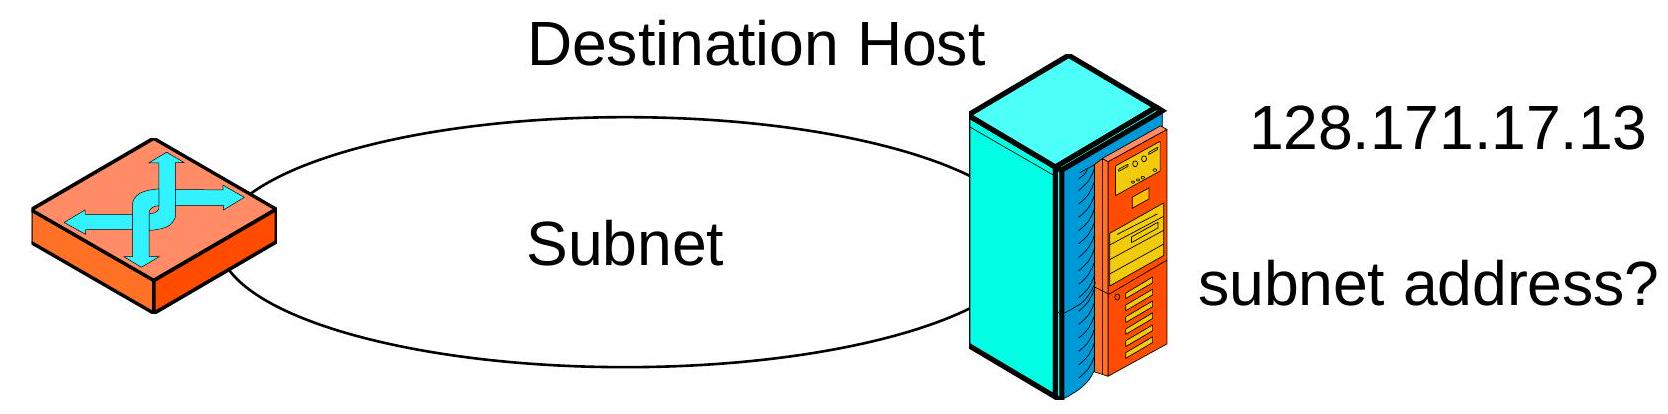
\includegraphics[max width=\textwidth]{2023_01_13_b07e3b4bcffdaab9792bg-169(1)}
\end{center}


\os{newpage} item[{\rot\bf  Address Resolution Protocol (ARP) }]~\\[-3ex]

\bi
  \ite Router creates an ARP Request message to be
sent to all hosts on the subnet.

  \ite Address resolution protocol message asks “Who has IP address 128.171.17.13?"

  \ite Passes ARP request to data link layer process for delivery

\ei

\begin{center}
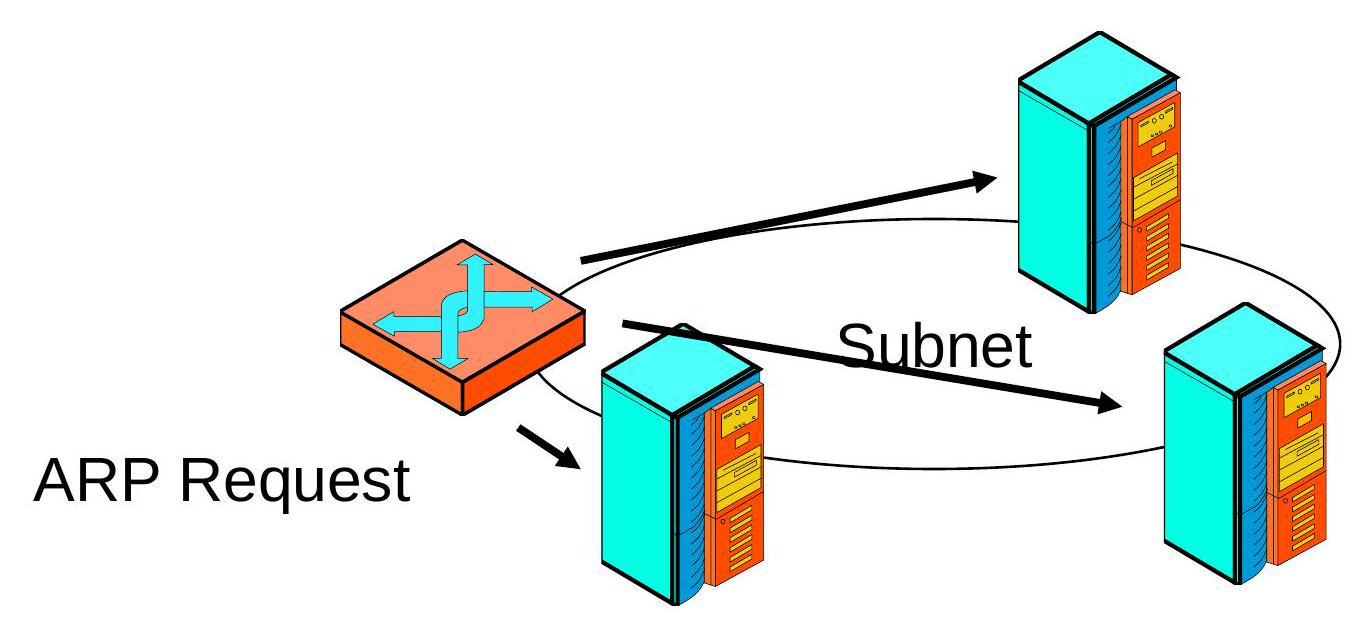
\includegraphics[max width=\textwidth]{2023_01_13_b07e3b4bcffdaab9792bg-170}
\end{center}


\os{newpage} item[{\rot\bf  Address Resolution Protocol (ARP) }]~\\[-3ex]


\os{newpage} item[{\rot\bf  - Data link process of router broadcasts the ARP Request message to all hosts on the subnet. }]~\\[-3ex]


\os{newpage} item[{\rot\bf  o On a LAN, MAC address of 48 ones tells all stations to pay attention to the frame }]~\\[-3ex]

\begin{center}
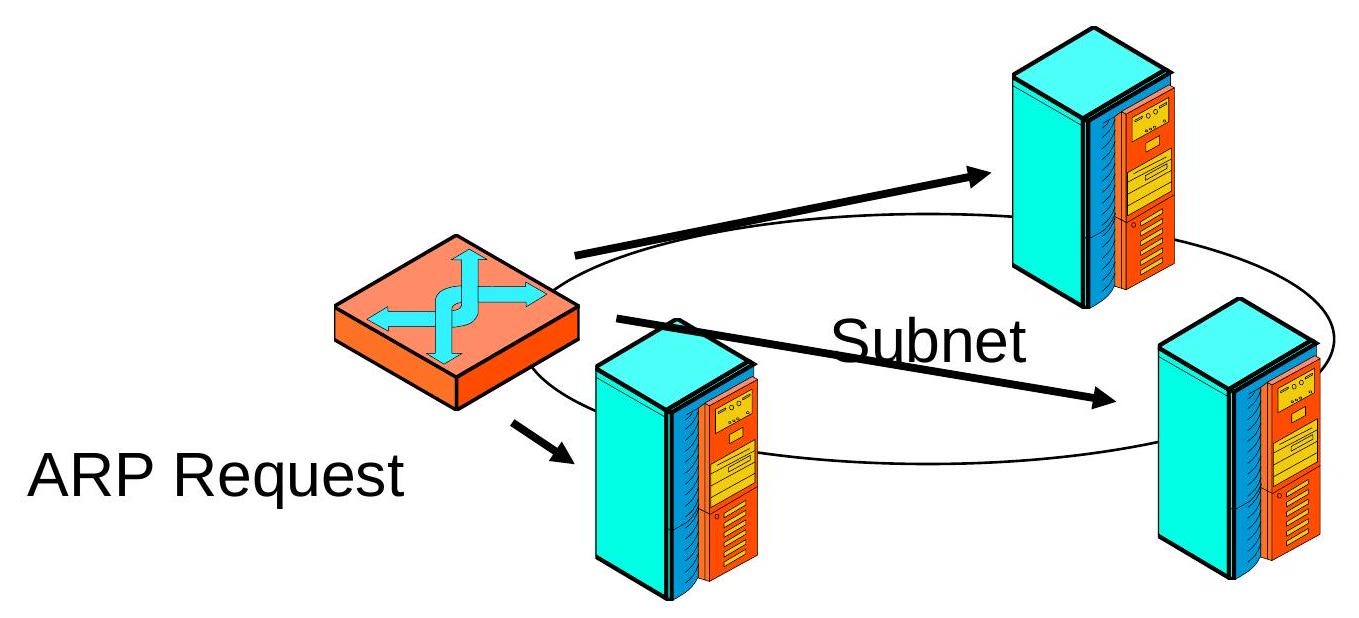
\includegraphics[max width=\textwidth]{2023_01_13_b07e3b4bcffdaab9792bg-171}
\end{center}


\os{newpage} item[{\rot\bf  Address Resolution Protocol ) }]~\\[-3ex]

\bi
  \ite Host with IP address 128.171.17.13 responds

  \ite Internet process creates an ARP response message

  \ite Contains the destination host's subnet address (48-bit MAC address on a LAN)
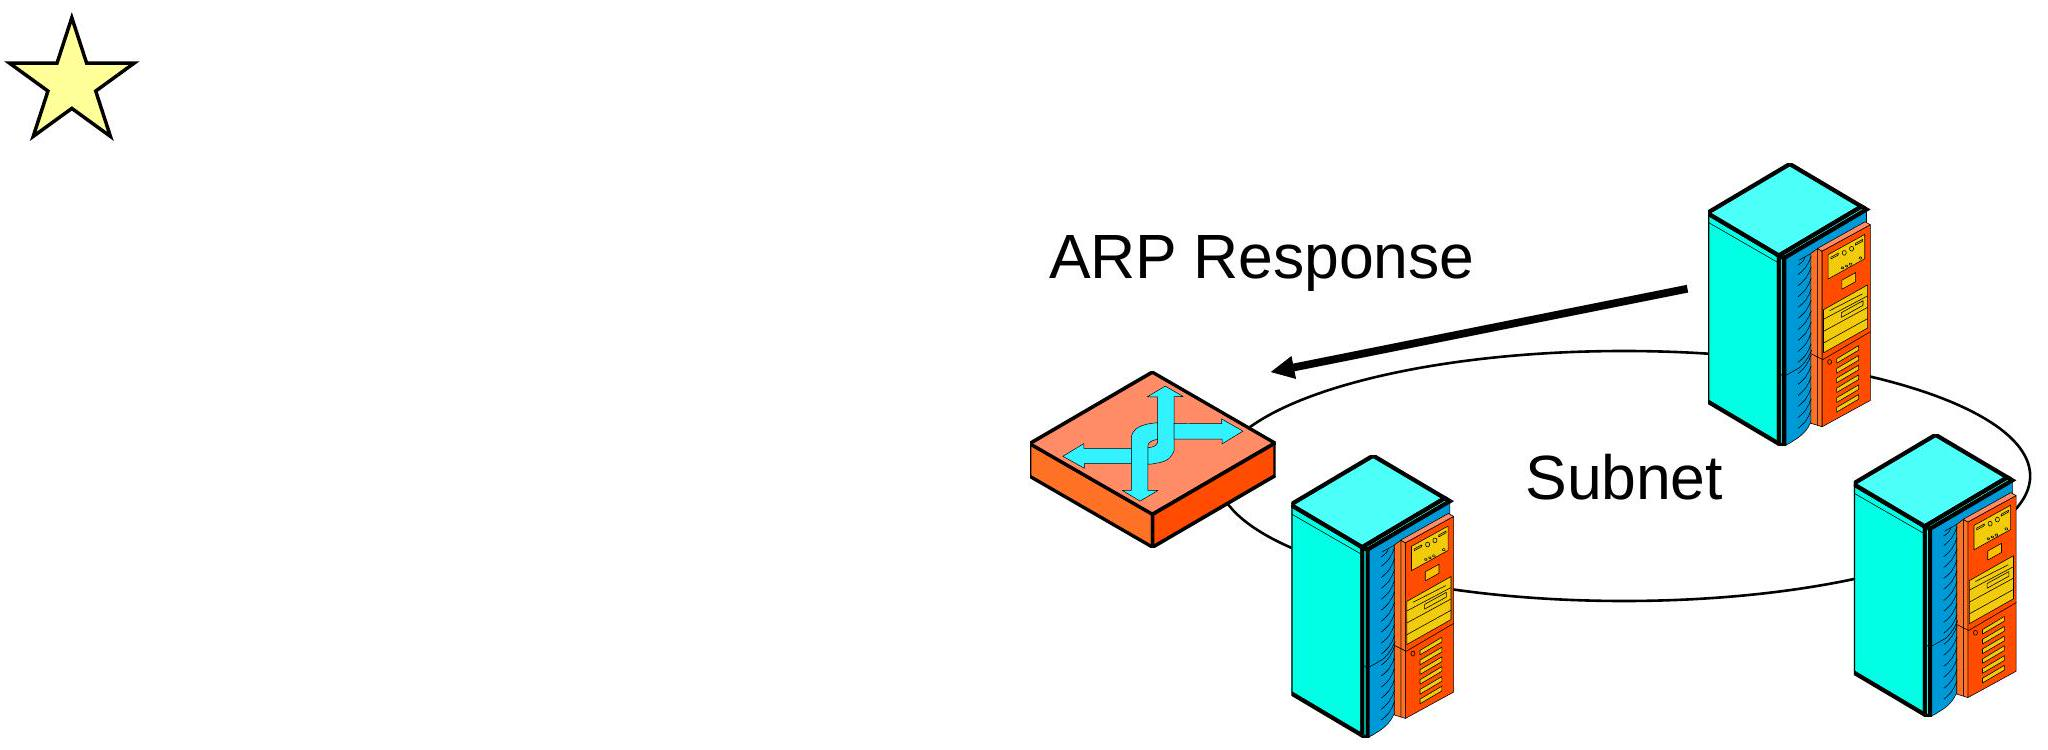
\includegraphics[max width=\textwidth, center]{2023_01_13_b07e3b4bcffdaab9792bg-172}

\ei


\item[{\rot\bf  Address Resolution Protocol  }]~\\[-3ex]

\bi
  \ite Router delivers the IP packet to the destination host
\ei
\bi
 \ite Places the IP packet in the subnet frame
 \ei

\bi
 \ite Puts the destination host's subnet address in the destination address field of the frame
 \ei


\begin{center}
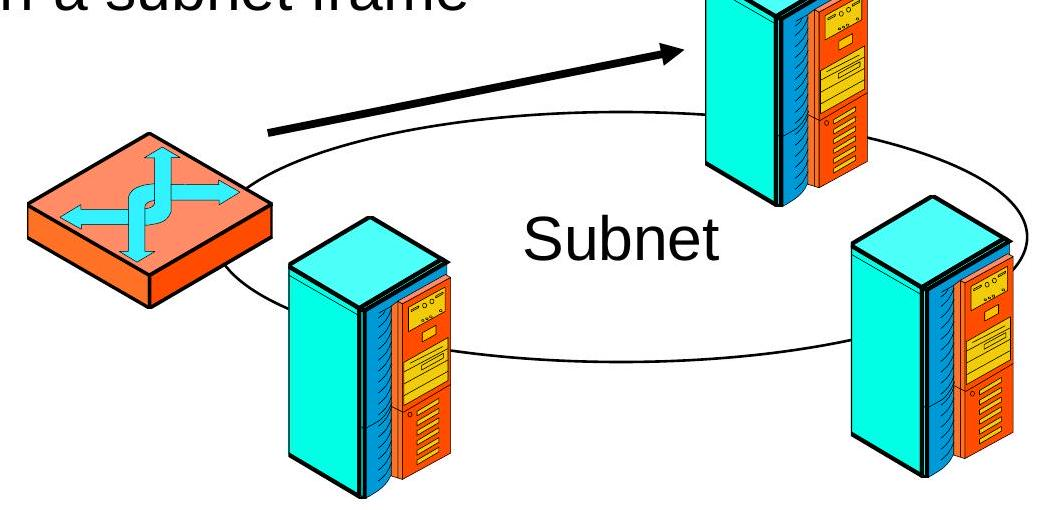
\includegraphics[max width=\textwidth]{2023_01_13_b07e3b4bcffdaab9792bg-173}
\end{center}


\os{newpage} item[{\rot\bf  Address Resolution Protocol }]~\\[-3ex]

\bi
  \ite ARP Requests and Responses are sent between thr
internet layer processes on the router and the
destination host
\ei

Router

\begin{center}

\includegraphics[max width=\textwidth]{2023_01_13_b07e3b4bcffdaab9792bg-174}
\end{center}

ARP

Request

\begin{center}
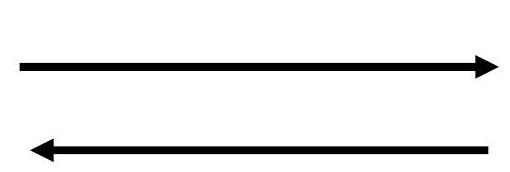
\includegraphics[max width=\textwidth]{2023_01_13_b07e3b4bcffdaab9792bg-174(1)}
\end{center}

ARP

Response Destination Host

Internet
Process

\section{Address Resolution Protocol
 - However, the data link processes deliver these ARP packets
 o Router broadcasts the ARP Request
 o Destination host sends ARP response to the subnet source address found in the broadcast frame}
Router

\begin{center}
\begin{tabular}{|c|}
\hline
Internet \\
Process \\
\hline
Data Link \\
Process \\
\hline
\end{tabular}
\end{center}

Broadcast ARP Request

\begin{center}
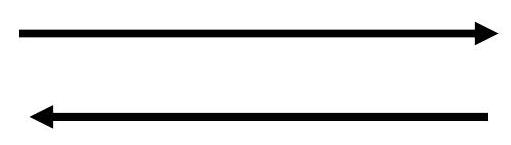
\includegraphics[max width=\textwidth]{2023_01_13_b07e3b4bcffdaab9792bg-175}
\end{center}

Direct ARP Response Destination Host

Data Link

Process


\item[{\rot\bf  Direct and Indirect Routing  }]~\\[-3ex]


\os{newpage} item[{\rot\bf  - Direct - when nodes are on the same network }]~\\[-3ex]


\os{newpage} item[{\rot\bf  - Indirect - used when the network numbers of the source and destination do not match }]~\\[-3ex]




\os{newpage} item[{\rot\bf  Transmission Control Protocol (TCP) }]~\\[-3ex]


\os{newpage} item[{\rot\bf  TCP: OvervieW RFCs: 793, 1122, 1323, 2018, 2581 }]~\\[-3ex]

\begin{center}
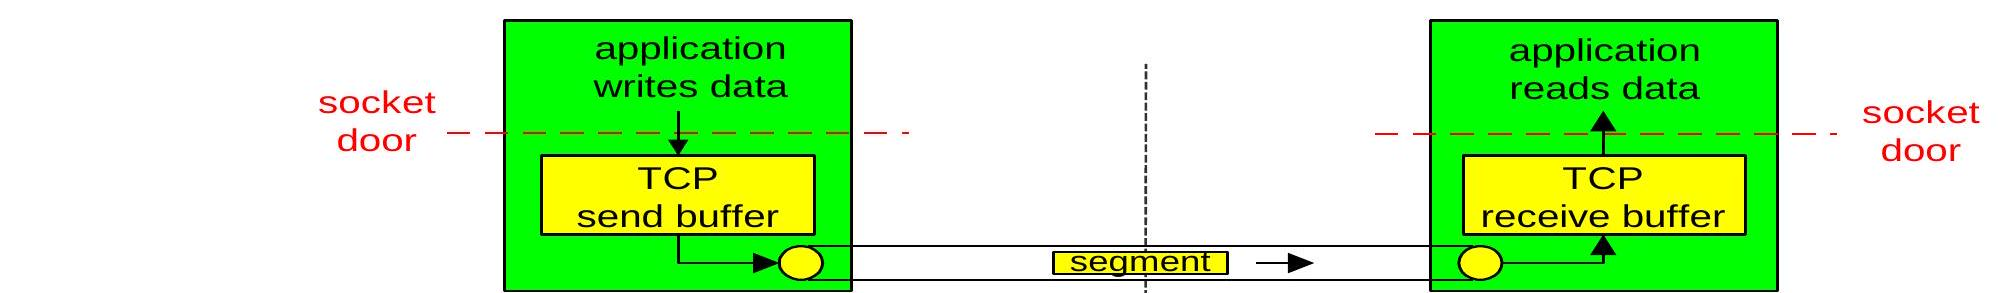
\includegraphics[max width=\textwidth]{2023_01_13_b07e3b4bcffdaab9792bg-178}
\end{center}

\bi
  \ite point-to-point (unicast):
\ei
\bi
 \ite one sender, one receiver
 \ei


\bi
  \ite connection-oriented:

  \ite handshaking (exchange of control msgs) init's sender, receiver state before data exchange

  \ite State resides only at the END systems - Not a virtual circuit!

  \ite full duplex data:

  \ite bi-directional data flow in same connection (A->B \& B->A in the same connection)

\ei
\bi
 \ite MSS: maximum segment size - reliable, in-order byte steam: o no "message boundaries"
 \ei


\bi
  \ite send \& receive buffers o buffer incoming \& outgoing data

  \ite flow controlled:

\ei
\bi
 \ite sender will not overwhelm receiver
 \ei


\bi
  \ite congestion controlled:
\ei
\bi
 \ite sender will not overwhelm network
 \ei



\os{newpage} item[{\rot\bf  TCP segment structure }]~\\[-3ex]


\os{newpage} item[{\rot\bf  2 bits }]~\\[-3ex]

URG: urgent data (generally not used)

ACK: ACK \# valid

PSH: push data now (generally not used)

RST, SYN, FIN: connection estab (setup, teardown commands)

Internet checksum (as in UDP)
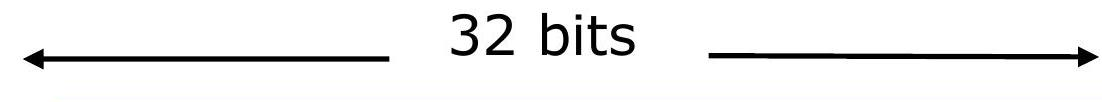
\includegraphics[max width=\textwidth, center]{2023_01_13_b07e3b4bcffdaab9792bg-179}

\begin{center}
\begin{tabular}{|c|c|}
\hline
source port \# & dest port \# \\
\hline
\end{tabular}
\end{center}

by bytes

of data

(not segments!)

$$
\begin{aligned}
& \text { application } \\
& \text { data } \\
& \text { (variable length) }
\end{aligned}
$$

\# bytes

rcvr willing

to accept


\os{newpage} item[{\rot\bf  TCP Connection-oriented demux }]~\\[-3ex]

\bi
  \ite TCP socket identified by 4 -tuple:
\ei
\bi
 \ite source IP address
 \ei

\bi
 \ite source port number
 \ei

\bi
 \ite dest IP address
 \ei

\bi
 \ite dest port number
 \ei



\os{newpage} item[{\rot\bf  - receiving host uses all four values to direct segment to appropriate socket }]~\\[-3ex]


\os{newpage} item[{\rot\bf  TCP Demultiplexing Example }]~\\[-3ex]

\begin{center}
\begin{tabular}{|l|l|l|l|l|l|}
\hline
 &  &  &  \\
\hline
\end{tabular}
\end{center}


\os{newpage} item[{\rot\bf  Typical TCP Transaction }]~\\[-3ex]

\begin{center}
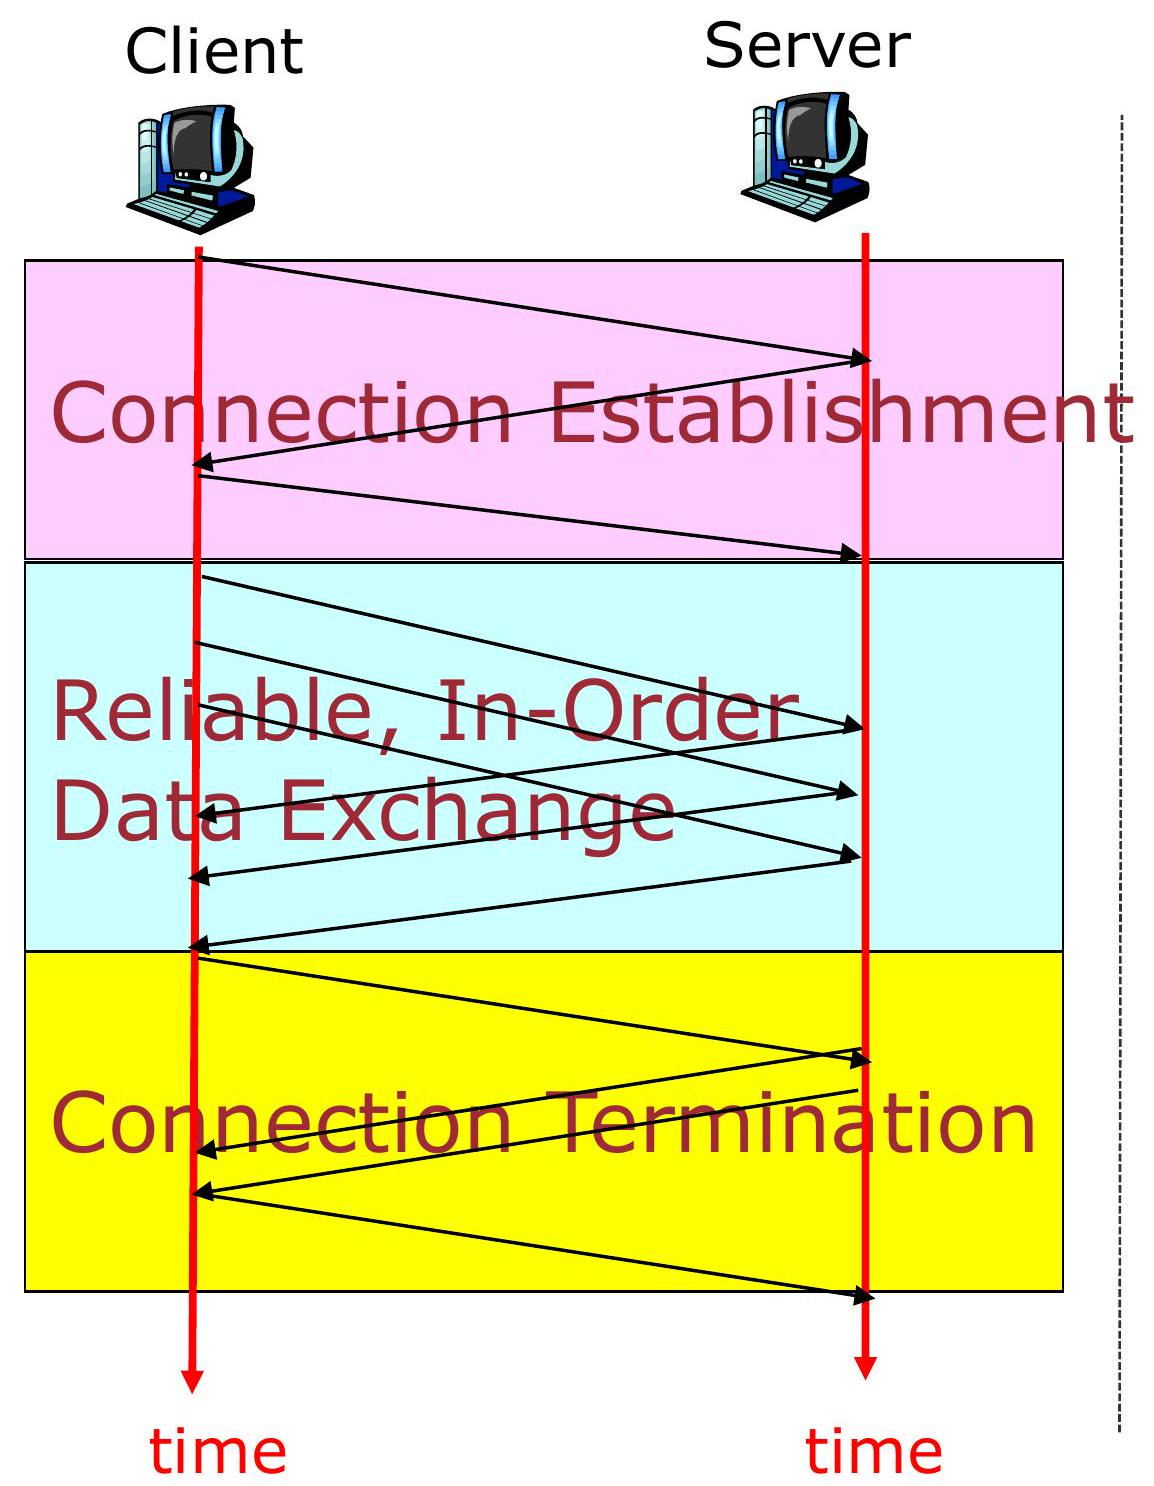
\includegraphics[max width=\textwidth]{2023_01_13_b07e3b4bcffdaab9792bg-182}
\end{center}


\os{newpage} item[{\rot\bf  A TCP Transaction consists of 3 Phases }]~\\[-3ex]

\begin{enumerate}
  \ite Connection Establishment
\end{enumerate}
\bi
 \ite Handshaking between client and server
 \ei



\os{newpage} item[{\rot\bf  Reliable, In-Order Data Exchange }]~\\[-3ex]
\bi
 \ite Recover any lost data through retransmissions and ACKs
 \ei



\os{newpage} item[{\rot\bf  Connection Termination o Closing the connection }]~\\[-3ex]


\os{newpage} item[{\rot\bf  TCP Connection Establishment }]~\\[-3ex]

\bi
  \ite TCP sender, receiver establish "connection" before exchanging data segments

  \ite initialize TCP variables:

\ei
\bi
 \ite seq. \#s
 \ei

\bi
 \ite buffers, flow control info (e.g. RcvWindow)
 \ei


\bi
  \ite client: connection initiator
\ei

Socket clientSocket $=$ new Socket ("hostname", port\#);

\bi
  \ite server: contacted by client Socket connectionSocket $=$ welcomeSocket. accept () ;
\ei


\os{newpage} item[{\rot\bf  Connection Establishment (cont) }]~\\[-3ex]


\os{newpage} item[{\rot\bf  Three way handshake: }]~\\[-3ex]

Step 1: client host sends TCP SYN segment to server
\bi
 \ite specifies a random initial seq \#
 \ei

\bi
 \ite no data
 \ei


Step 2: server host receives SYN, replies with SYNACK segment o server allocates buffers
\bi
 \ite specifies server initial seq. \# Step 3: client receives SYNACK, replies with $\mathrm{ACK}$ segment, which may contain data
 \ei


\begin{center}
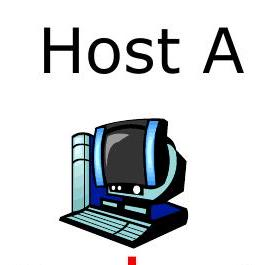
\includegraphics[max width=\textwidth]{2023_01_13_b07e3b4bcffdaab9792bg-184}
\end{center}

Host B

Conhection

request $\sqrt{S Y N, S_{e q}=42} \quad$ host ACKs and selects its own initial seq \#


\os{newpage} item[{\rot\bf  Connection Establishment (cont) }]~\\[-3ex]


\os{newpage} item[{\rot\bf  Seq. \#'s: }]~\\[-3ex]
\bi
 \ite byte stream "number" of first byte in segment's data
 \ei



\os{newpage} item[{\rot\bf  ACKs: }]~\\[-3ex]

O seq \# of next byte expected from other side
\bi
 \ite cumulative ACK
 \ei


\begin{center}

\includegraphics[max width=\textwidth]{2023_01_13_b07e3b4bcffdaab9792bg-185}
\end{center}

Host B

Connection

request

\begin{center}
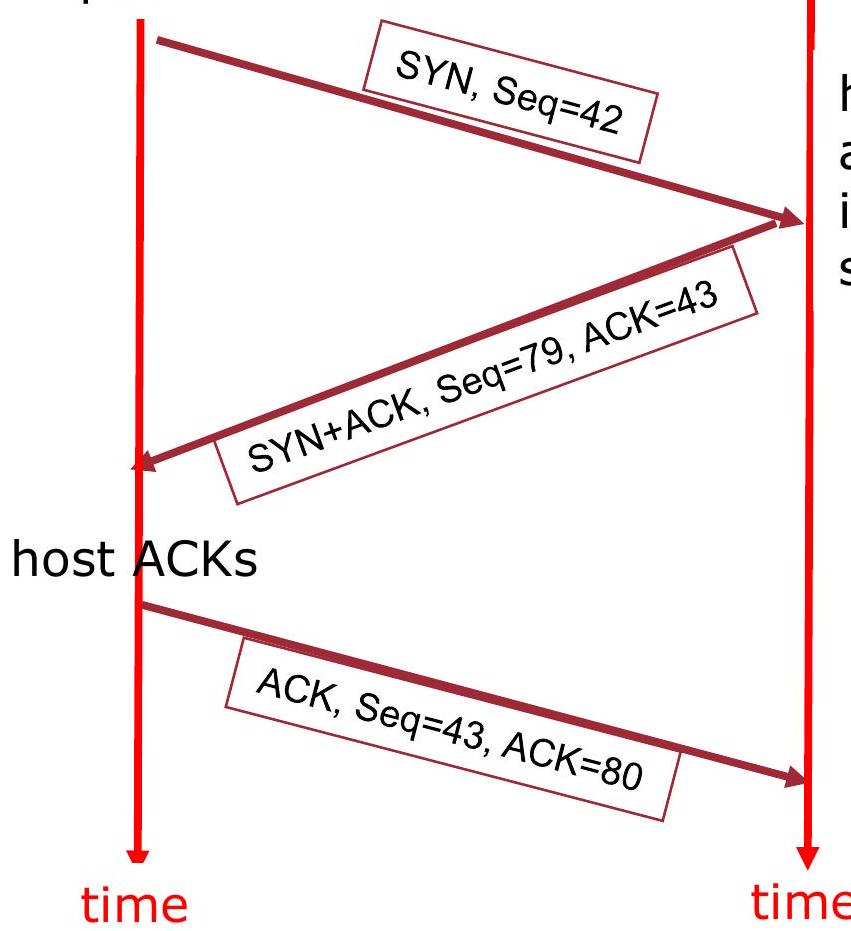
\includegraphics[max width=\textwidth]{2023_01_13_b07e3b4bcffdaab9792bg-185(1)}
\end{center}

host ACKs and selects its own initial seq \#

Three-way handshake


\os{newpage} item[{\rot\bf  TCP Starting Sequence Number Selection }]~\\[-3ex]

\bi
  \ite Why a random starting sequence \#? Why not simply choose o?

  \ite To protect against two incarnations of the same connection reusing the same sequence numbers too soon

  \ite That is, while there is still a chance that a segment from an earlier incarnation of a connection will interfere with a later incarnation of the connection

  \ite How?

  \ite Client machine seq \#o, initiates connection to server with seq \#0.

  \ite Client sends one byte and client machine crashes

  \ite Client reboots and initiates connection again

  \ite Server thinks new incarnation is the same as old connection

\ei


\os{newpage} item[{\rot\bf  TCP Connection Termination }]~\\[-3ex]


\os{newpage} item[{\rot\bf  Closing a connection: }]~\\[-3ex]

client closes socket:

clientSocket. close () ;


\os{newpage} item[{\rot\bf  Step 1: client end system sends TCP FIN control segment to server }]~\\[-3ex]

Step 2: server receives FIN, replies with $\mathrm{ACK}$. Server might send some buffered but not sent data before closing the connection. Server then sends FIN and moves to Closing state.

\begin{center}
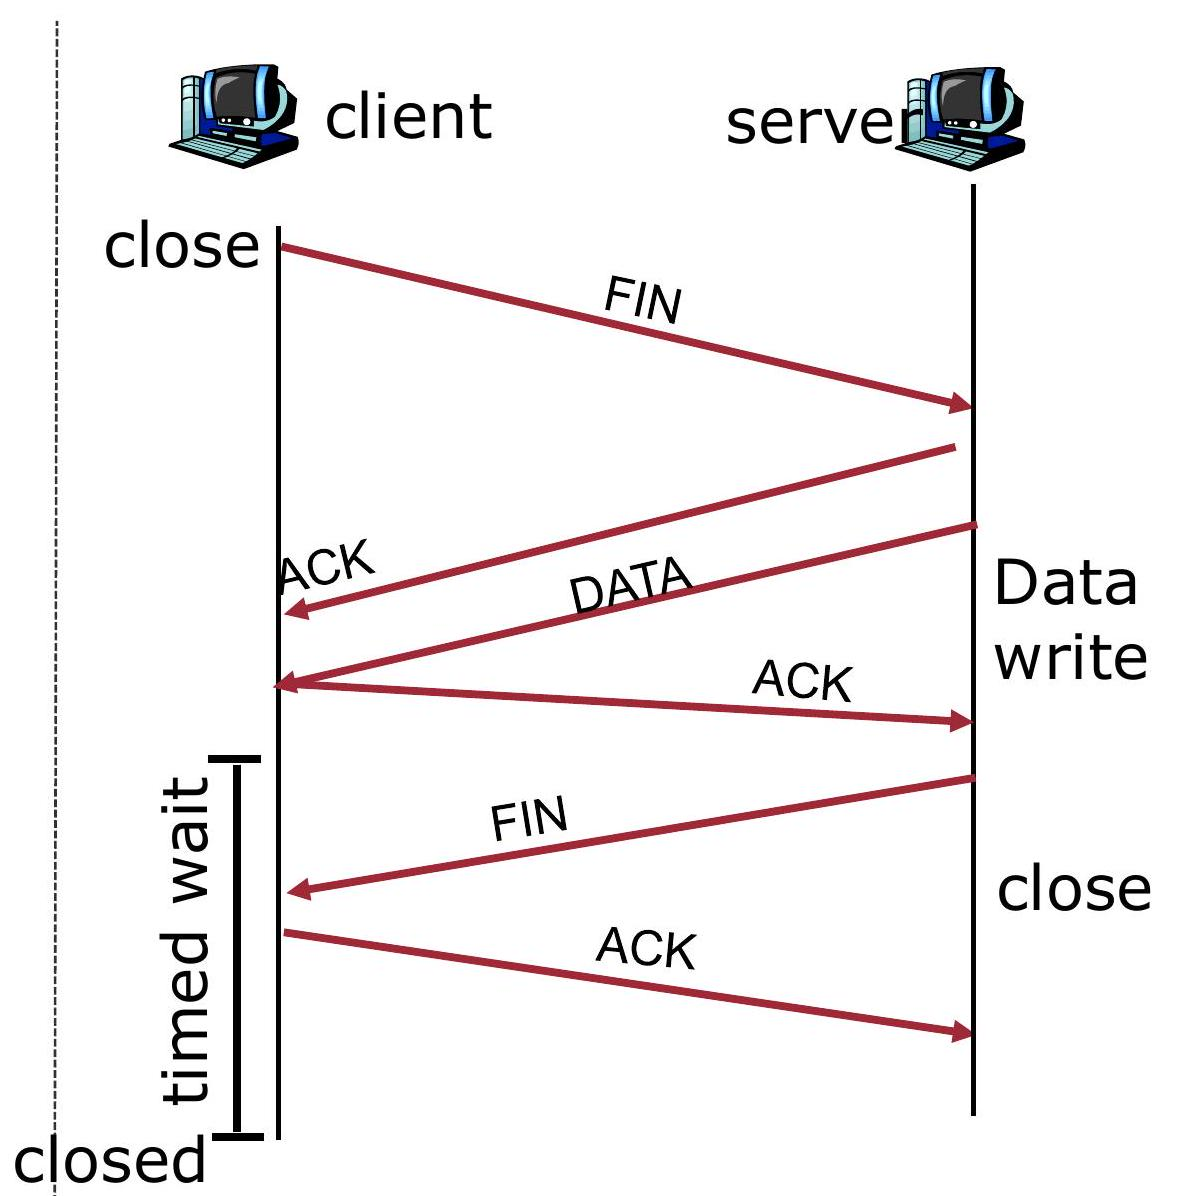
\includegraphics[max width=\textwidth]{2023_01_13_b07e3b4bcffdaab9792bg-187}
\end{center}


\os{newpage} item[{\rot\bf  TCP Connection Termination }]~\\[-3ex]

Step 3: client receives FIN, replies with ACK.
\bi
 \ite Enters "timed wait" - will respond with ACK to received FINs
 \ei


Step 4: server, receives ACK. Connection closed.

\bi
  \ite Why wait before closing the connection?

  \ite If the connection were allowed to move to CLOSED state, then another pair of application processes might come along and open the same connection (use the same port \#s) and a delayed FIN from an earlier incarnation would terminate the connection.

\ei

\begin{center}
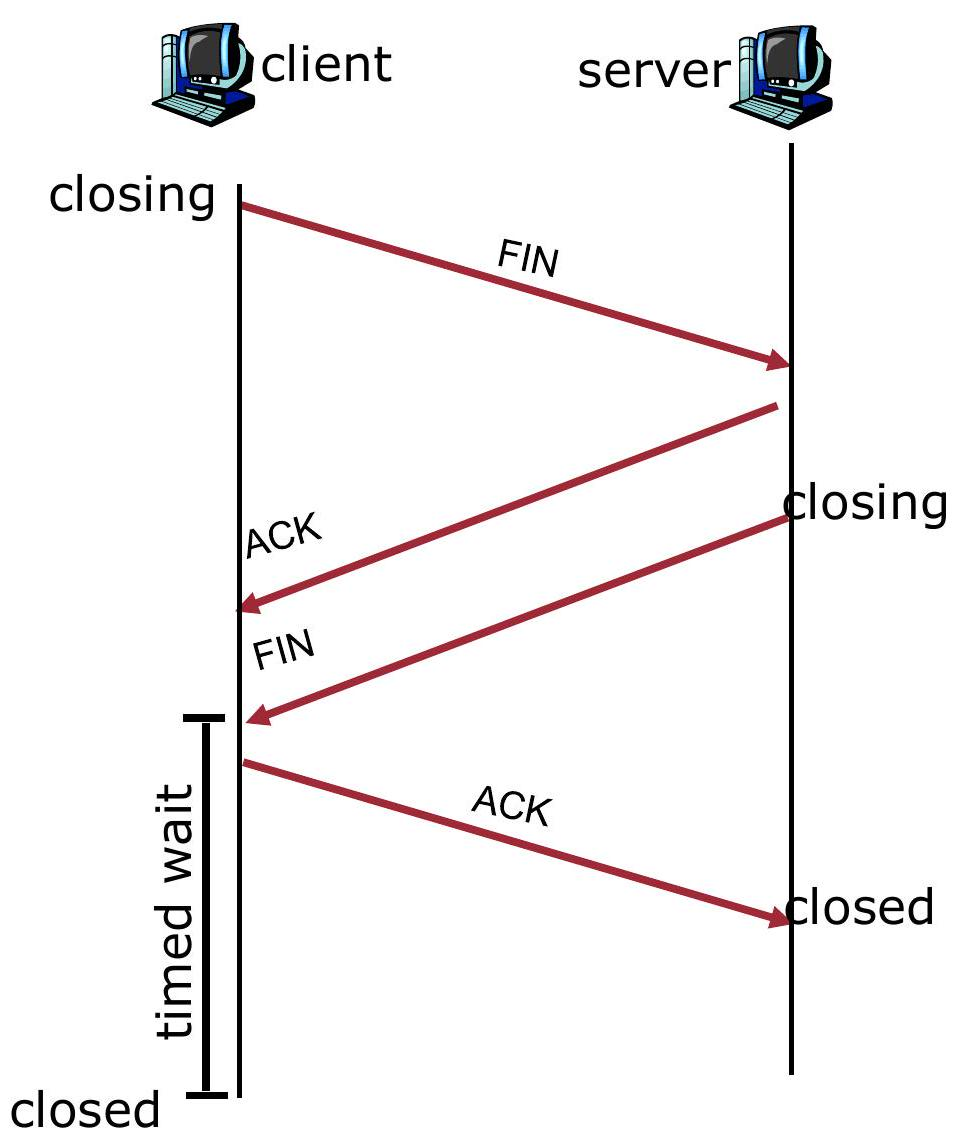
\includegraphics[max width=\textwidth]{2023_01_13_b07e3b4bcffdaab9792bg-188}
\end{center}


\os{newpage} item[{\rot\bf  TCP State-Transition Diagram }]~\\[-3ex]

\begin{center}
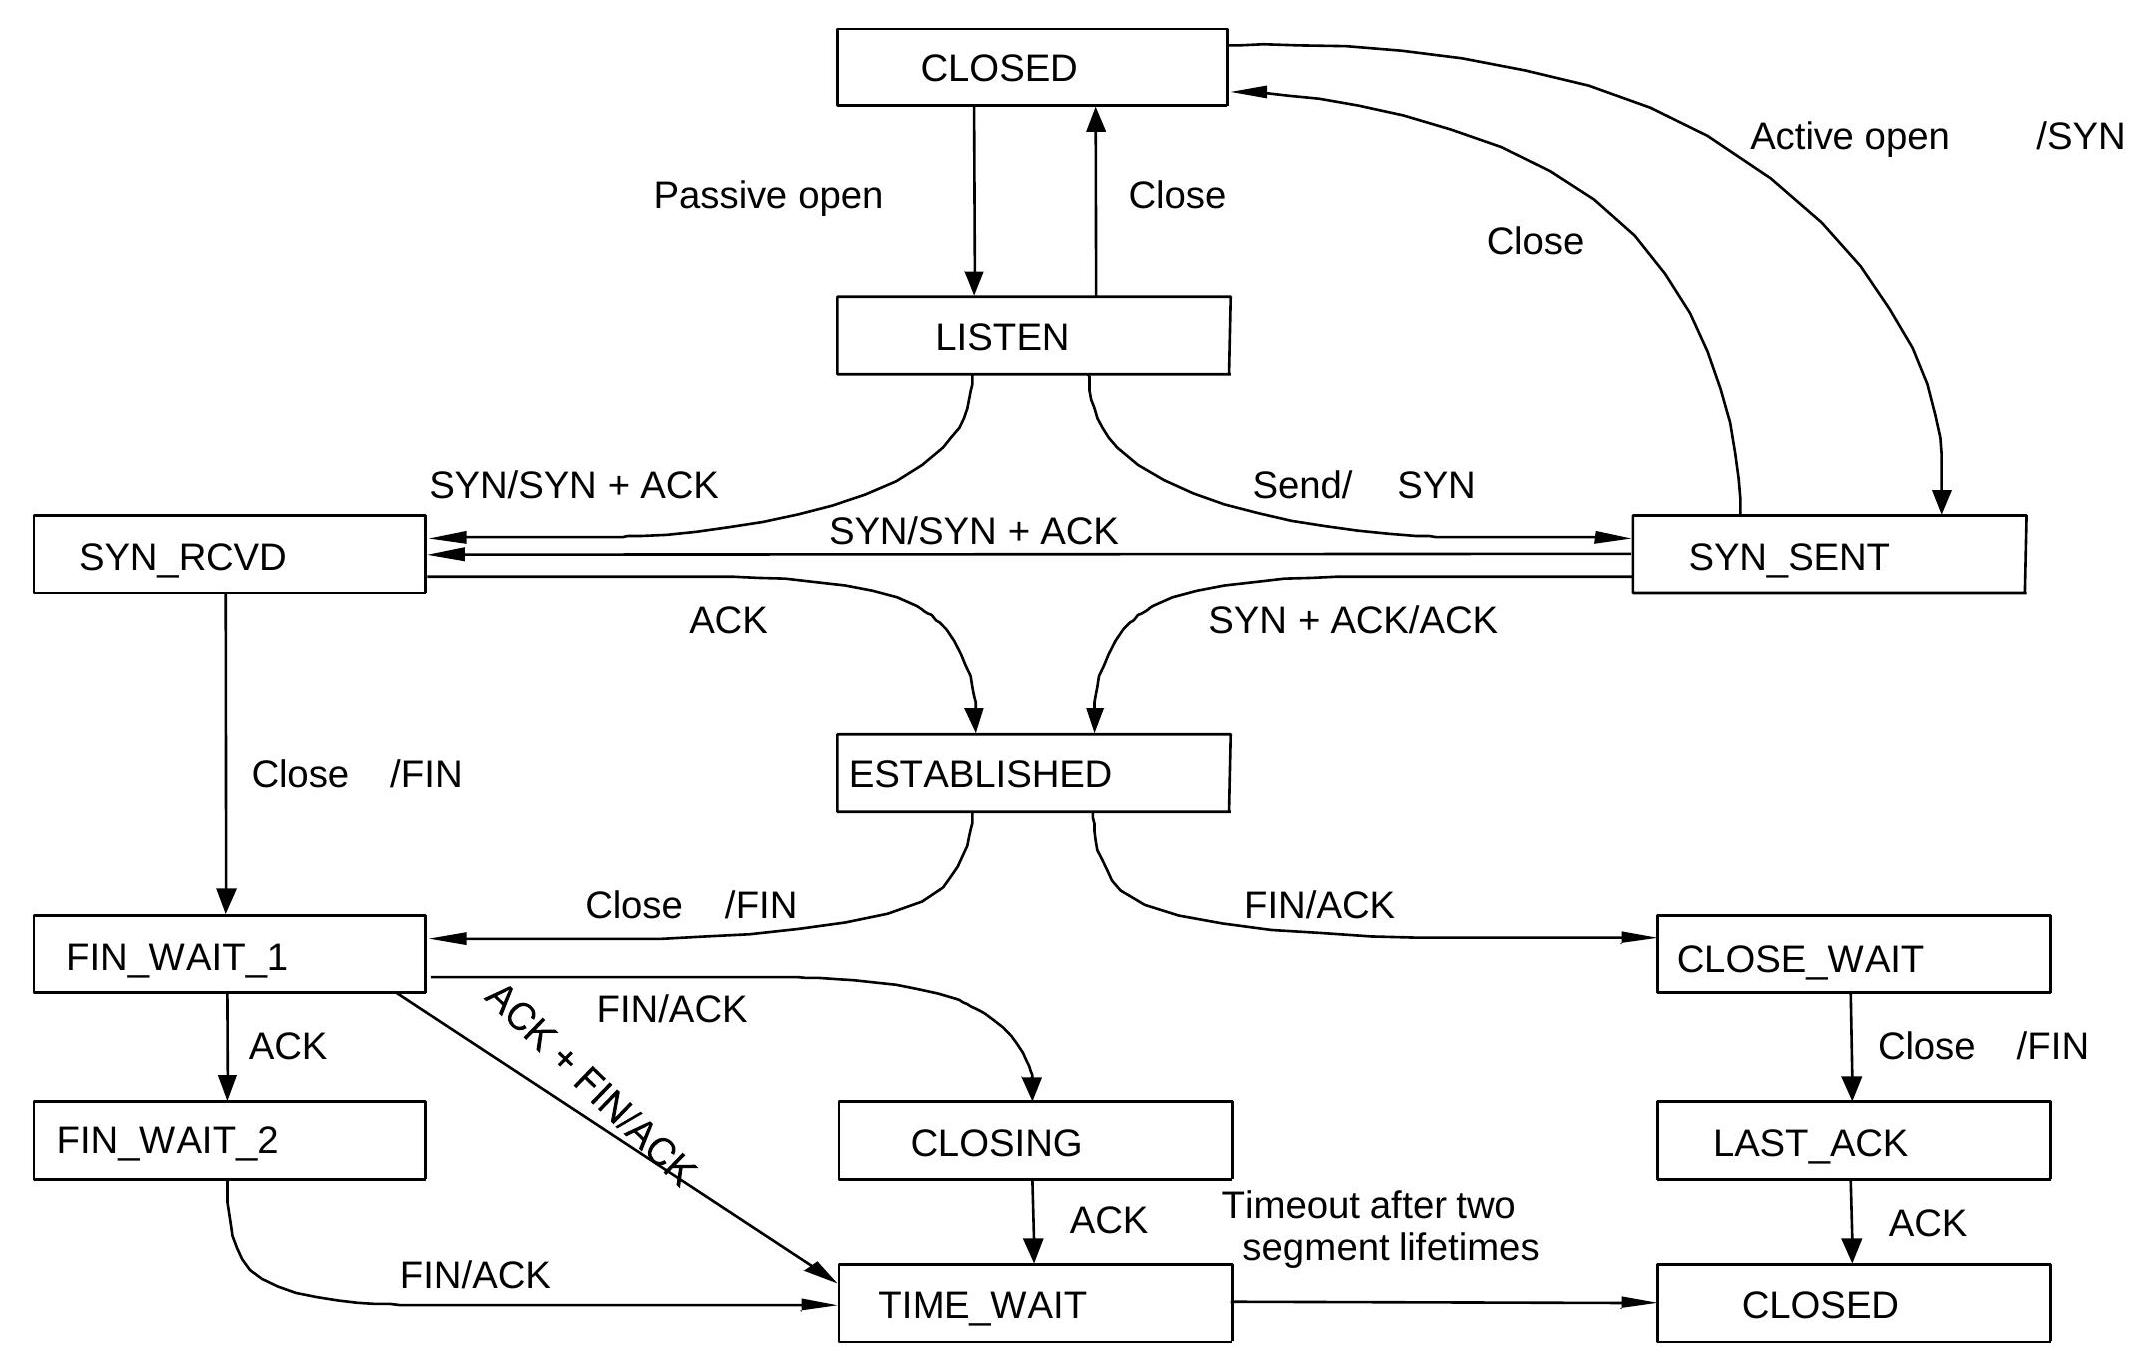
\includegraphics[max width=\textwidth]{2023_01_13_b07e3b4bcffdaab9792bg-189}
\end{center}


\os{newpage} item[{\rot\bf  Typical TCP Client/Server Transitions }]~\\[-3ex]

\begin{center}
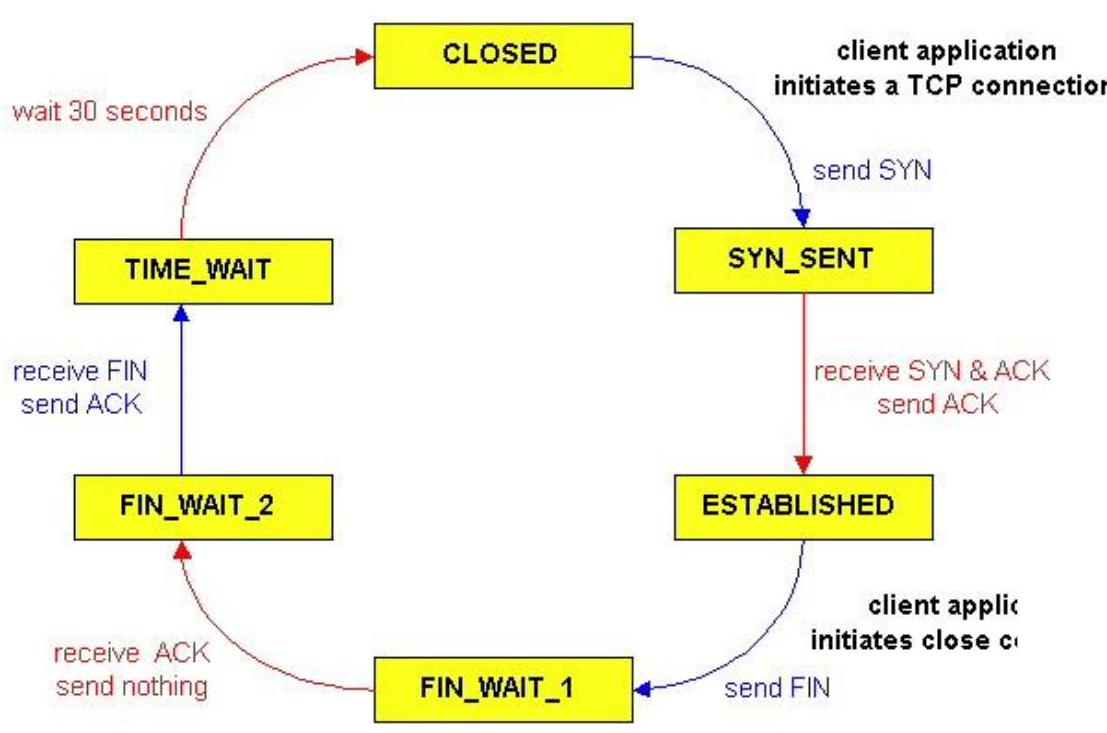
\includegraphics[max width=\textwidth]{2023_01_13_b07e3b4bcffdaab9792bg-190}
\end{center}

TCP client

lifecycle TCP server lifecycle

\begin{center}
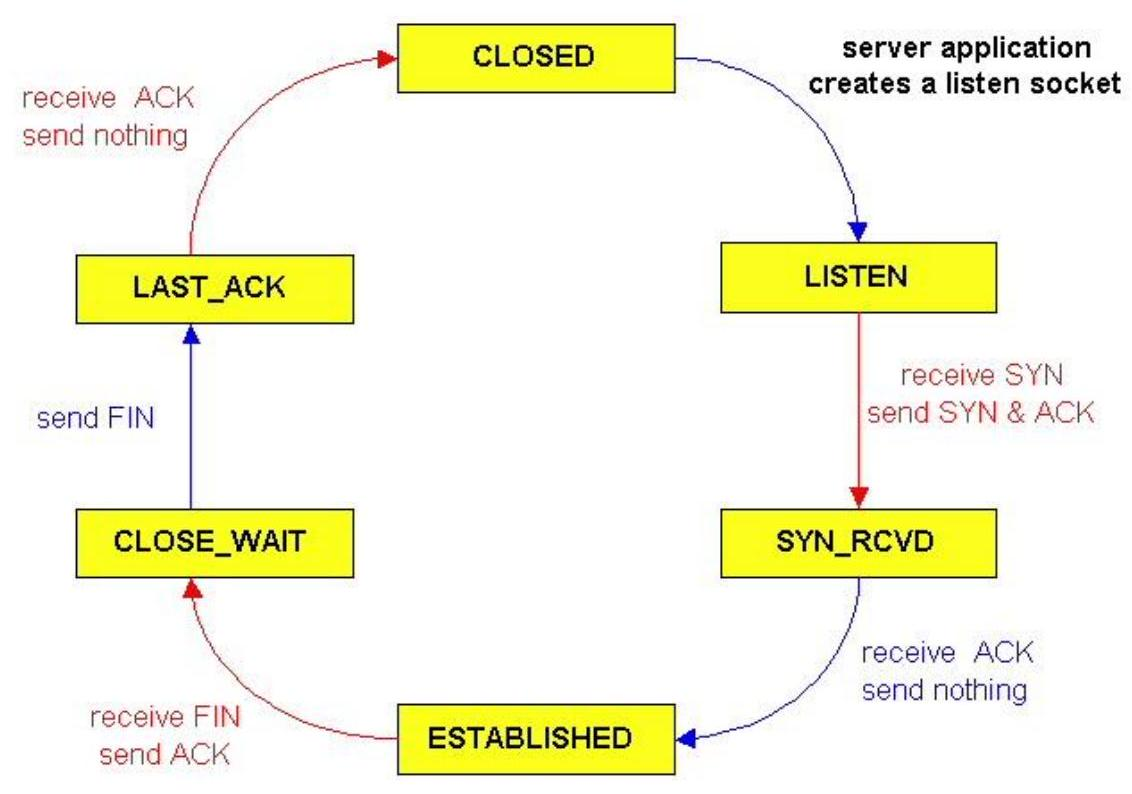
\includegraphics[max width=\textwidth]{2023_01_13_b07e3b4bcffdaab9792bg-190(1)}
\end{center}


\os{newpage} item[{\rot\bf  How to program using the TCP? }]~\\[-3ex]

\begin{center}
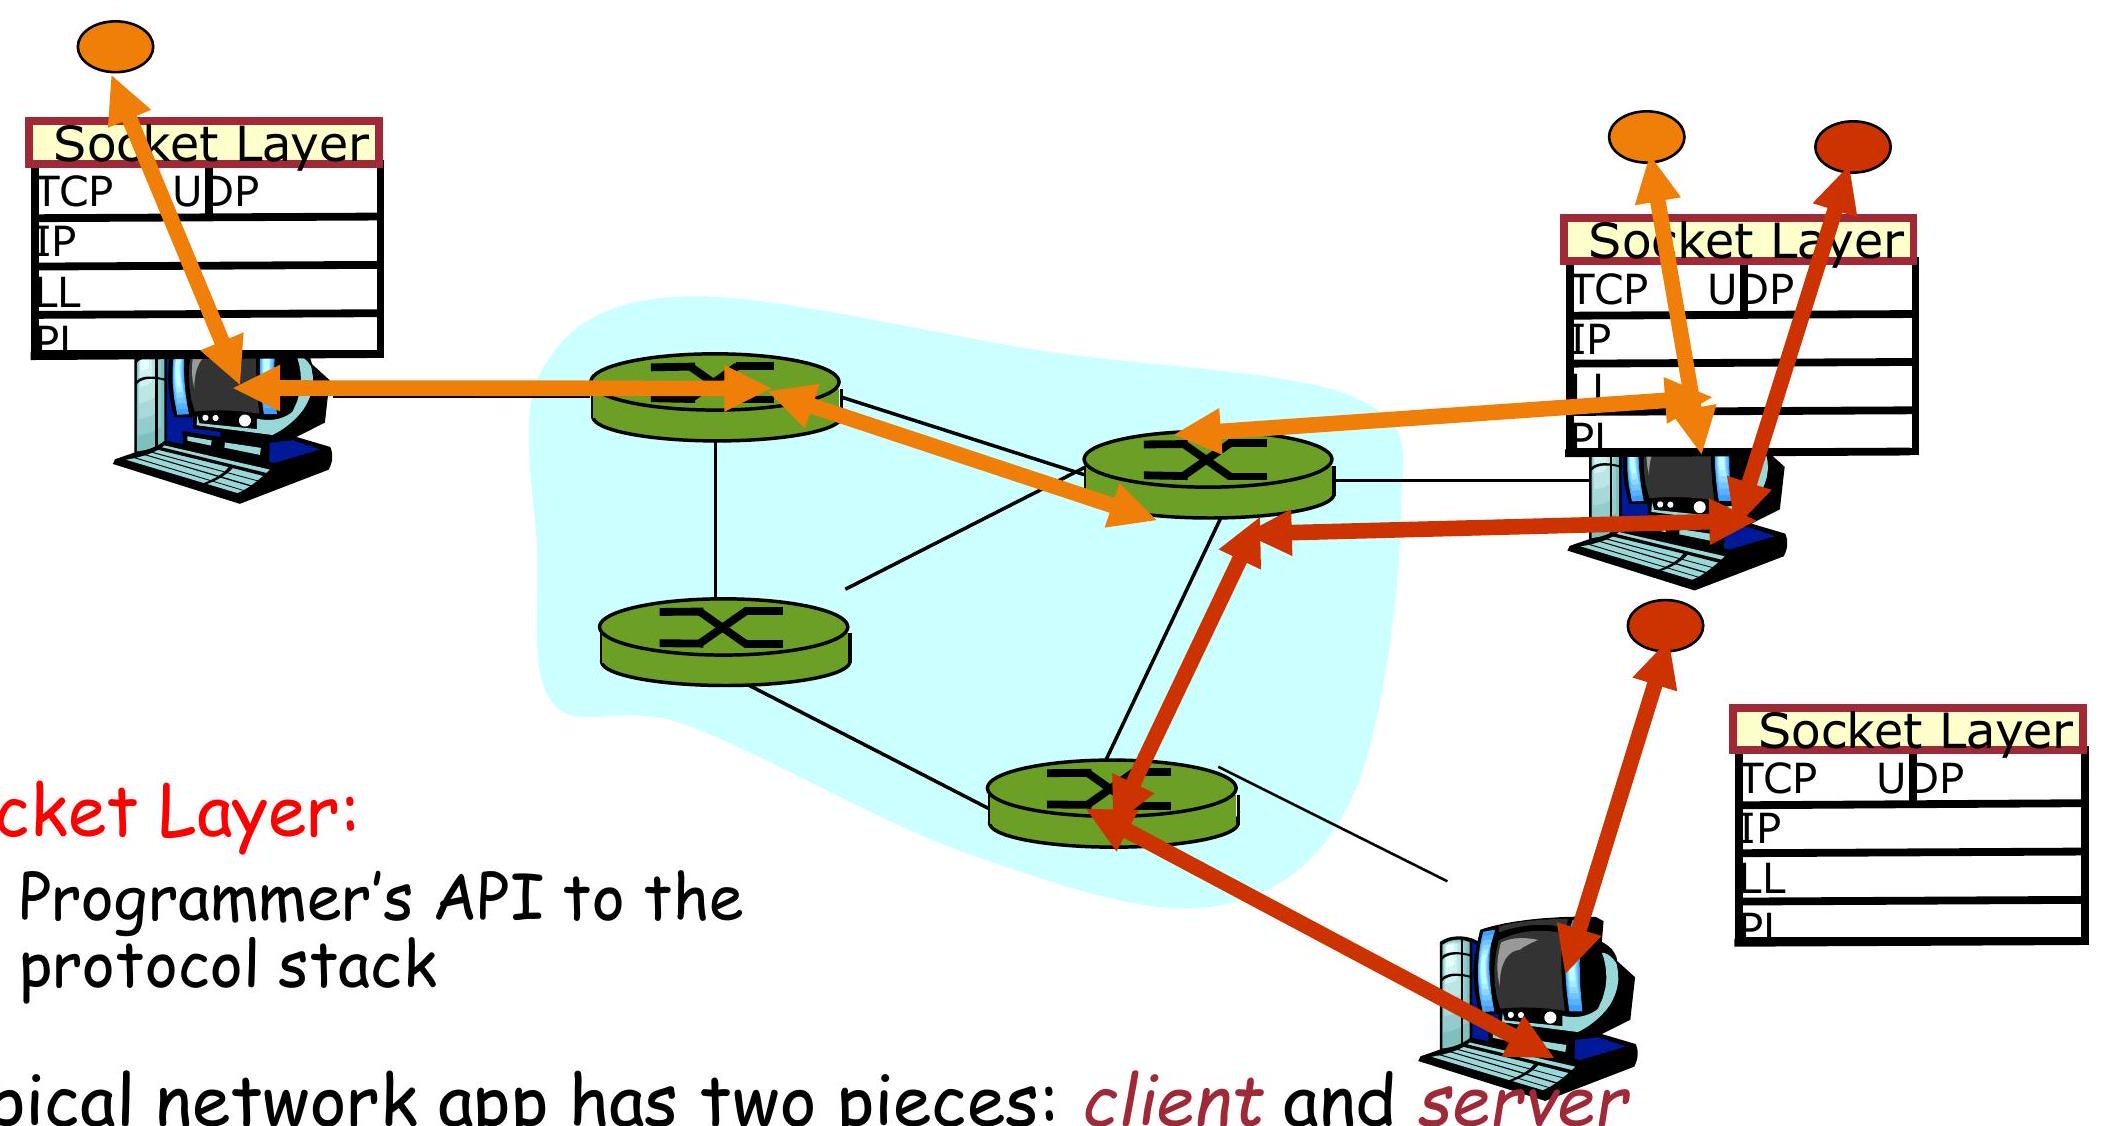
\includegraphics[max width=\textwidth]{2023_01_13_b07e3b4bcffdaab9792bg-191}
\end{center}
\bi
 \ite Programmer's API to the protocol stack
 \ei


$\square$ Typical network app has two pieces: client and server Server: Passive entity. Provides service to clients
\bi
 \ite e.g., Web server responds with the requested Web page
 \ei


$\square$ Client: initiates contact with server ("speaks first")
\bi
 \ite typically requests service from server, e.9., Web Browser
 \ei



\os{newpage} item[{\rot\bf  Socket Creation }]~\\[-3ex]

\bi
  \ite mySock = socket(family, type, protocol);

  \ite UDP/TCP/IP-specific sockets

\ei

\begin{center}
\begin{tabular}{|l|c|c|l|}
\multicolumn{2}{c}{Family} & Type & Protocol \\
\hline
TCP & \multirow{3}{*}{PF\_INET} & SOCK\_STREAM & IPPROTO\_TCP \\
\cline { 3 - 4 }
 &  & SOCK\_DGRAM & IPPROTO\_UDP \\
\hline
UDP &  &  &  \\
\hline
\end{tabular}
\end{center}

\bi
  \ite Socket reference
\ei
\bi
 \ite File (socket) descriptor in UNIX
 \ei

\bi
 \ite Socket handle in WinSock
 \ei



\os{newpage} item[{\rot\bf  TCP Client/Server Interaction }]~\\[-3ex]

Server starts by getting ready to receive client connections...



\begin{enumerate}
  \ite Create a TCP socket

  \ite Establish connection

  \ite Communicate

  \ite Close the connection Server

\end{enumerate}

Create a TCP socket

Assign a port to socket

Set socket to listen

Repeatedly:

a. Accept new connection

b. Communicate

c. Close the connection


\os{newpage} item[{\rot\bf  TCP Client/Server Interaction }]~\\[-3ex]

$/ *$ Create socket for incoming connections */

if $(($ servSock $=$ socket(PF\_INET, SOCK\_STREAM, IPPROTO\_TCP $))<0)$ DieWithError("socket() failed");

Client

\begin{enumerate}
  \ite Create a TCP socket

  \ite Establish connection

  \ite Communicate

  \ite Close the connection Server

\end{enumerate}

Create a TCP socket

Bind socket to a port

Set socket to listen

Repeatedly:

a. Accept new connection

b. Communicate

c. Close the connection


\os{newpage} item[{\rot\bf  TCP Client/Server Interaction }]~\\[-3ex]

echoServAddr.sin\_family $=$ AF\_INET;

echoServAddr.sin\_addr.s\_addr $=$ htonl(INADDR\_ANY);/* Any incoming interface */ echoServAddr.sin\_port $=$ htons(echoServPort);

if (bind(servSock, (struct sockaddr DieWithError("bind() failed");


\os{newpage} item[{\rot\bf  Client }]~\\[-3ex]

\begin{enumerate}
  \ite $\quad$ Create a TCP socket

  \ite Establish connection

  \ite Communicate

  \ite Close the connection /* Internet address family \textit{/ /} Local port */

\end{enumerate}

Server

Create a TCP socket Bind socket to a port

Set socket to listen

Repeatedly:
a. Accept new connection
b. Communicate
c. Close the connection


\item[{\rot\bf  TCP Client/Server Interaction  }]~\\[-3ex]

Client

\begin{enumerate}
  \ite Create a TCP socket

  \ite Establish connection

  \ite Communicate

  \ite Close the connection Server

\end{enumerate}

Create a TCP socket Bind socket to a port

Set socket to listen

Repeatedly:
a. Accept new connection
b. Communicate
c. Close the connection


\item[{\rot\bf  TCP Client/Server Interaction  }]~\\[-3ex]

\textbackslash author\{
for $(i ;) / *$ Run forever $* /$ \textbackslash  \{ \textbackslash  clntLen $=$ sizeof(echoCIntAddr $)$; \textbackslash  if $(($ clntSock=accept(servSock, (struct sockaddr * $)$ \&echoCIntAddr, \&clntLen $))<0)$ \textbackslash  DieWithError("accept() failed");
\}


\os{newpage} item[{\rot\bf  Client }]~\\[-3ex]

\begin{enumerate}
  \ite Create a TCP socket

  \ite Establish connection

  \ite Communicate

  \ite Close the connection

\end{enumerate}


\os{newpage} item[{\rot\bf  Server }]~\\[-3ex]

Create a TCP socket Bind socket to a port Set socket to listen Repeatedly:
a. Accept new connection
b. Communicate
c. Close the connection


\os{newpage} item[{\rot\bf  TCP Client/Server Interaction }]~\\[-3ex]

Server is now blocked waiting for connection from a client



\begin{enumerate}
  \ite Create a TCP socket

  \ite Establish connection

  \ite Communicate

  \ite Close the connection

\end{enumerate}


\os{newpage} item[{\rot\bf  Server }]~\\[-3ex]

Create a TCP socket

Bind socket to a port

Set socket to listen

Repeatedly:
a. Accept new connection
b. Communicate
c. Close the connection


\os{newpage} item[{\rot\bf  TCP Client/Server Interaction }]~\\[-3ex]

Later, a client decides to talk to the server...



\begin{enumerate}
  \ite Create a TCP socket

  \ite Establish connection

  \ite Communicate

  \ite Close the connection Server

\end{enumerate}

Create a TCP socket

Bind socket to a port

Set socket to listen

Repeatedly:
a. Accept new connection
b. Communicate
c. Close the connection


\os{newpage} item[{\rot\bf  TCP Client/Server Interaction }]~\\[-3ex]

/* Create a reliable, stream socket using TCP */

if $(($ sock $=$ socket(PF\_INET, SOCK\_STREAM, IPPROTO\_TCP $))<0)$ DieWithError("socket() failed");


\os{newpage} item[{\rot\bf  Client }]~\\[-3ex]

\begin{enumerate}
  \ite Create a TCP socket

  \ite Establish connection

  \ite Communicate

  \ite Close the connection Server

\end{enumerate}

Create a TCP socket Bind socket to a port

Set socket to listen Repeatedly:

a. Accept new connection

b. Communicate

c. Close the connection


\item[{\rot\bf  TCP Client/Server Interaction  }]~\\[-3ex]

Client

\begin{enumerate}
  \ite Create a TCP socket

  \ite Establish connection

  \ite Communicate

  \ite Close the connection

\end{enumerate}


\os{newpage} item[{\rot\bf  Server }]~\\[-3ex]

Create a TCP socket

Bind socket to a port

Set socket to listen

Repeatedly:
a. Accept new connection
b. Communicate
c. Close the connection


\os{newpage} item[{\rot\bf  TCP Client/Server Interaction }]~\\[-3ex]

echoStringLen $=$ strlen $($ echoString $)$;

/* Determine input length * /

/* Send the string to the server $* /$

if (send(sock, echoString, echoStringLen, 0) $!=$ echoStringLen)

DieWithError("send() sent a different number of bytes than expected");

Client

\begin{enumerate}
  \ite Create a TCP socket

  \ite Establish connection

  \ite Communicate

  \ite Close the connection Server

\end{enumerate}

Create a TCP socket

\begin{enumerate}
  \setcounter{enumi}{1}
  \ite Bind socket to a port

  \ite Set socket to listen

  \ite Repeatedly:

\end{enumerate}

a. Accept new connection

b. Communicate

c. Close the connection


\os{newpage} item[{\rot\bf  TCP Client/Server Interaction }]~\\[-3ex]

/* Receive message from client */

if $(($ recvMsgSize $=\operatorname{recv}($ clntSocket, echoBuffer, RCVBUFSIZE, 0) $)<0)$ DieWithError("recv() failed");

Client

\begin{enumerate}
  \ite Create a TCP socket

  \ite Establish connection

  \ite Communicate

  \ite Close the connection Server

  \ite Create a TCP socket

\end{enumerate}

. Bind socket to a port

\begin{enumerate}
  \setcounter{enumi}{2}
  \ite Set socket to listen

  \ite Repeatedly:
a. Accept new connection
b. Communicate
c. Close the connection

\end{enumerate}


\os{newpage} item[{\rot\bf  TCP Client/Server Interaction }]~\\[-3ex]

close(sock);



\begin{enumerate}
  \ite Create a TCP socket

  \ite Establish connection

  \ite Communicate

  \ite Close the connection

\end{enumerate}


\os{newpage} item[{\rot\bf  close(clntSocket) }]~\\[-3ex]

Server

Create a TCP socket

Bind socket to a port

Set socket to listen

Repeatedly:

a. Accept new connection

b. Communicate

c. Close the connection


\item[{\rot\bf  TCP Tidbits  }]~\\[-3ex]

\bi
  \ite Client knows server address and port

  \ite No correlation between send () and recv ()

\ei

Server

$\operatorname{recv}()->$ "Hello"

$\operatorname{recv}()->$ "Bob"

send("Hi ")

send("Jane")

$\operatorname{recv}()->$ "Hi Jane"


\os{newpage} item[{\rot\bf  Serial Busses }]~\\[-3ex]

\begin{center}
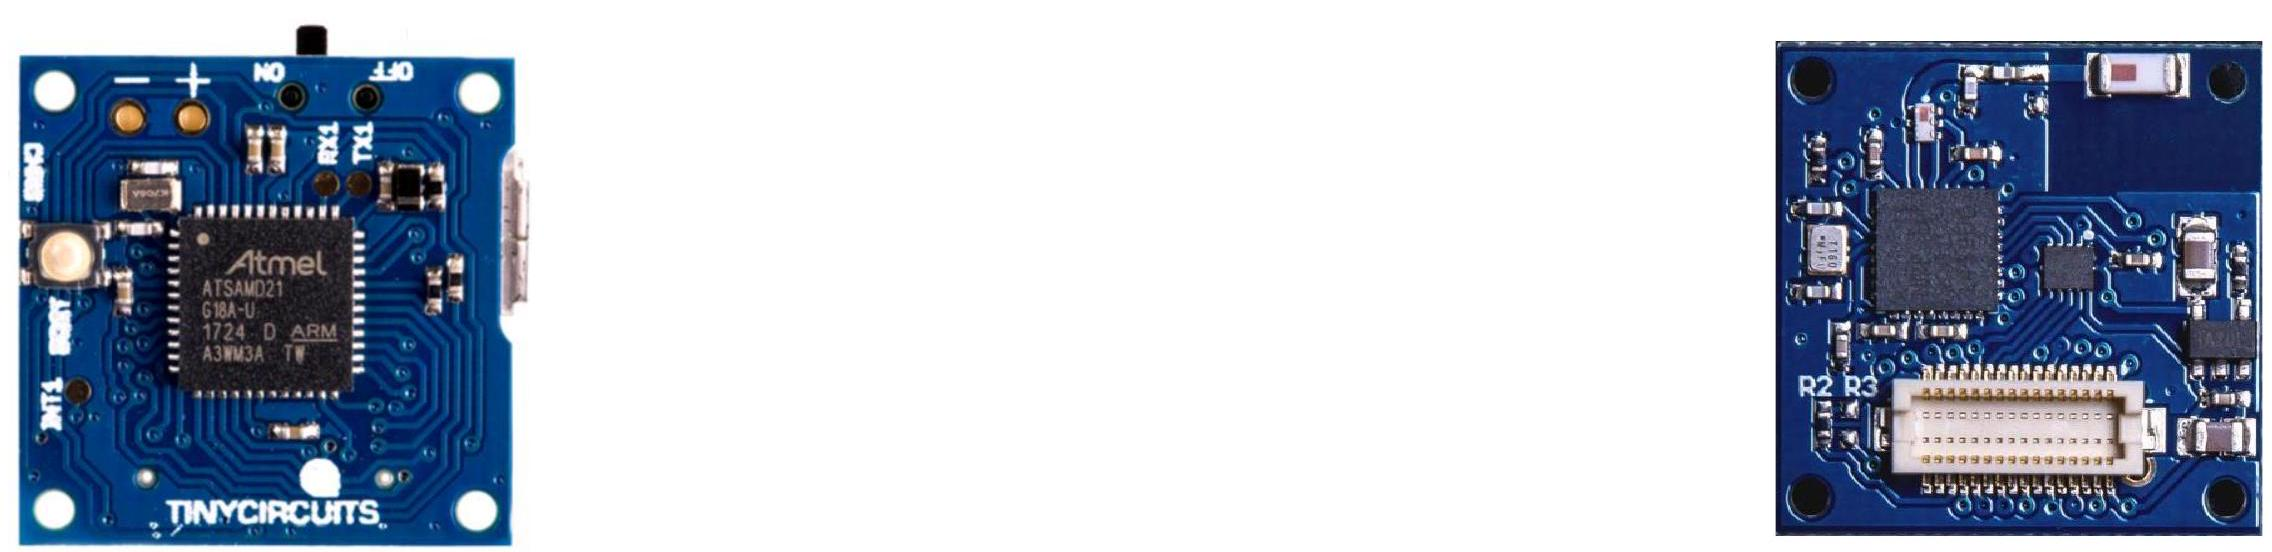
\includegraphics[max width=\textwidth]{2023_01_13_b07e3b4bcffdaab9792bg-206}
\end{center}


\os{newpage} item[{\rot\bf  Serial Buses in Embedded }]~\\[-3ex]

\bi
  \ite UART serial bus for sending debug messages to your
development host

  \ite I2C serial bus for communicating with sensors (e.g., the accelerometer)

\ei


\os{newpage} item[{\rot\bf  - SPI serial bus for communicating with the Bluetooth Low Energy radio }]~\\[-3ex]


\os{newpage} item[{\rot\bf  Serial Interfaces }]~\\[-3ex]

\begin{center}
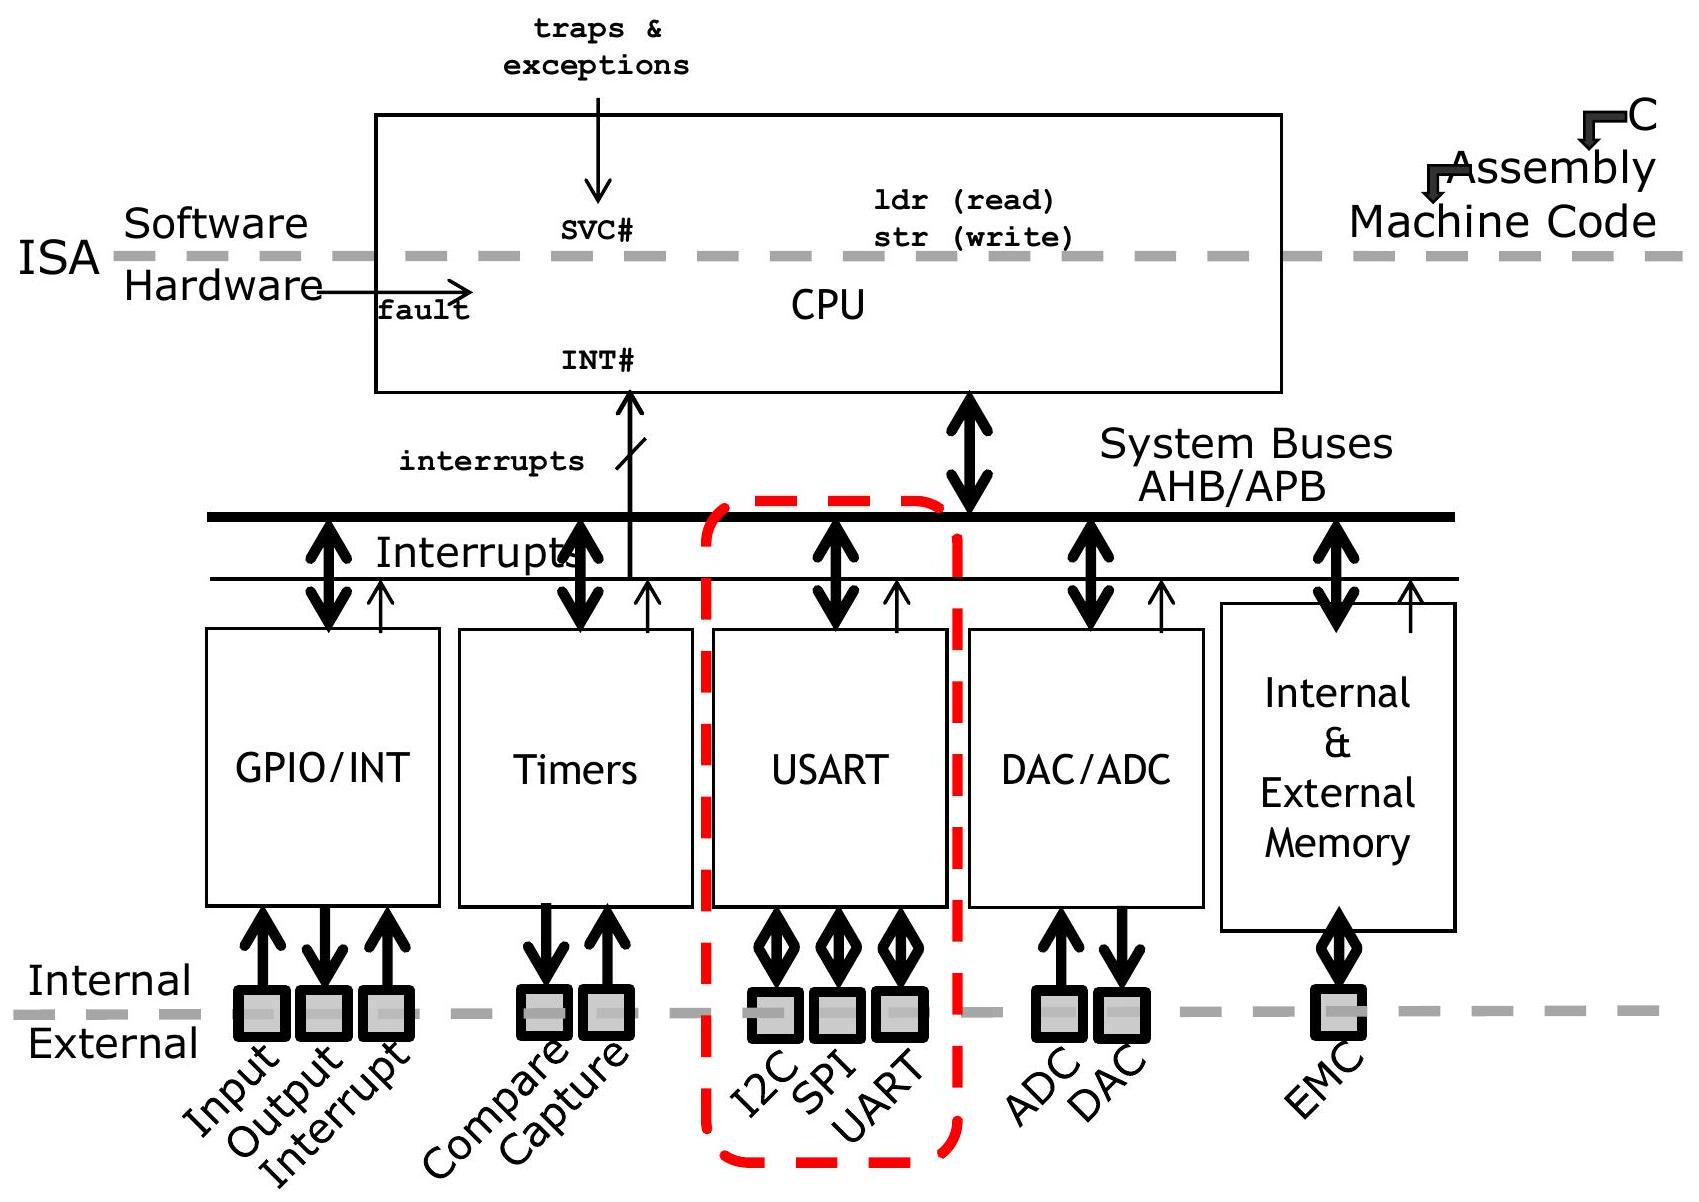
\includegraphics[max width=\textwidth]{2023_01_13_b07e3b4bcffdaab9792bg-208}
\end{center}


\os{newpage} item[{\rot\bf  Parallel Bus VS Serial Bus }]~\\[-3ex]

\begin{center}
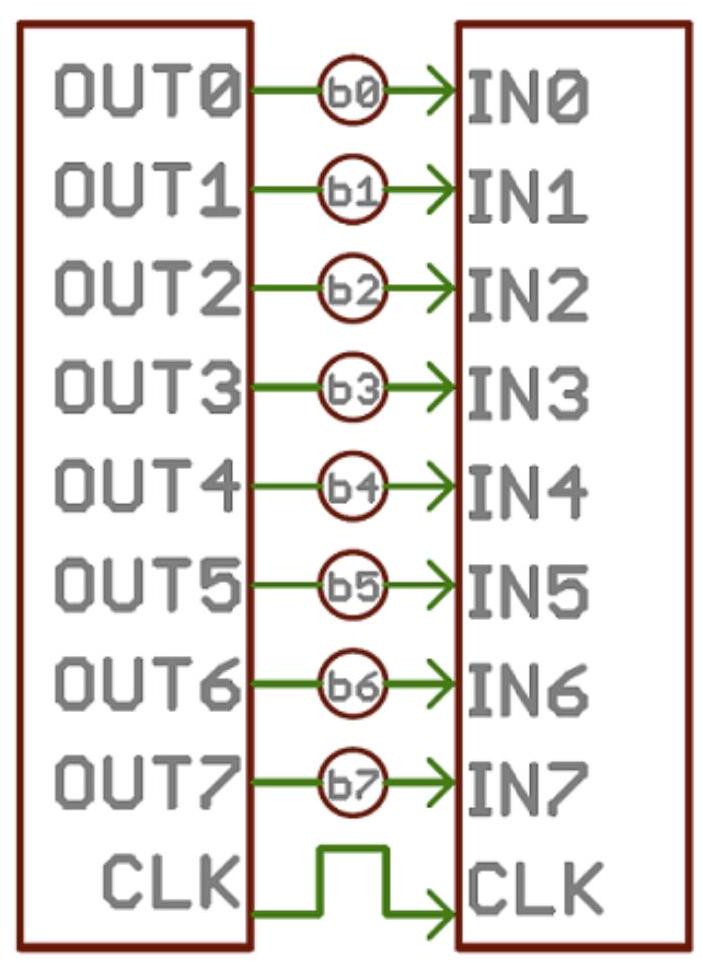
\includegraphics[max width=\textwidth]{2023_01_13_b07e3b4bcffdaab9792bg-209}
\end{center}

\begin{center}
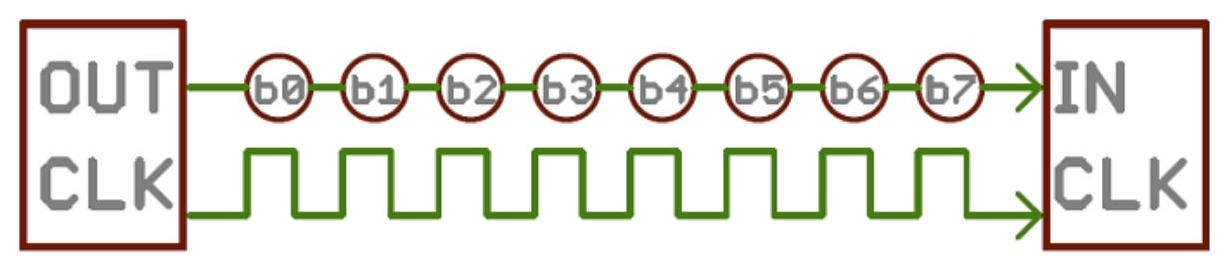
\includegraphics[max width=\textwidth]{2023_01_13_b07e3b4bcffdaab9792bg-209(1)}
\end{center}

\section{Simplistic View of Serial Port Operation Transmitter
 Receiver}
\begin{center}
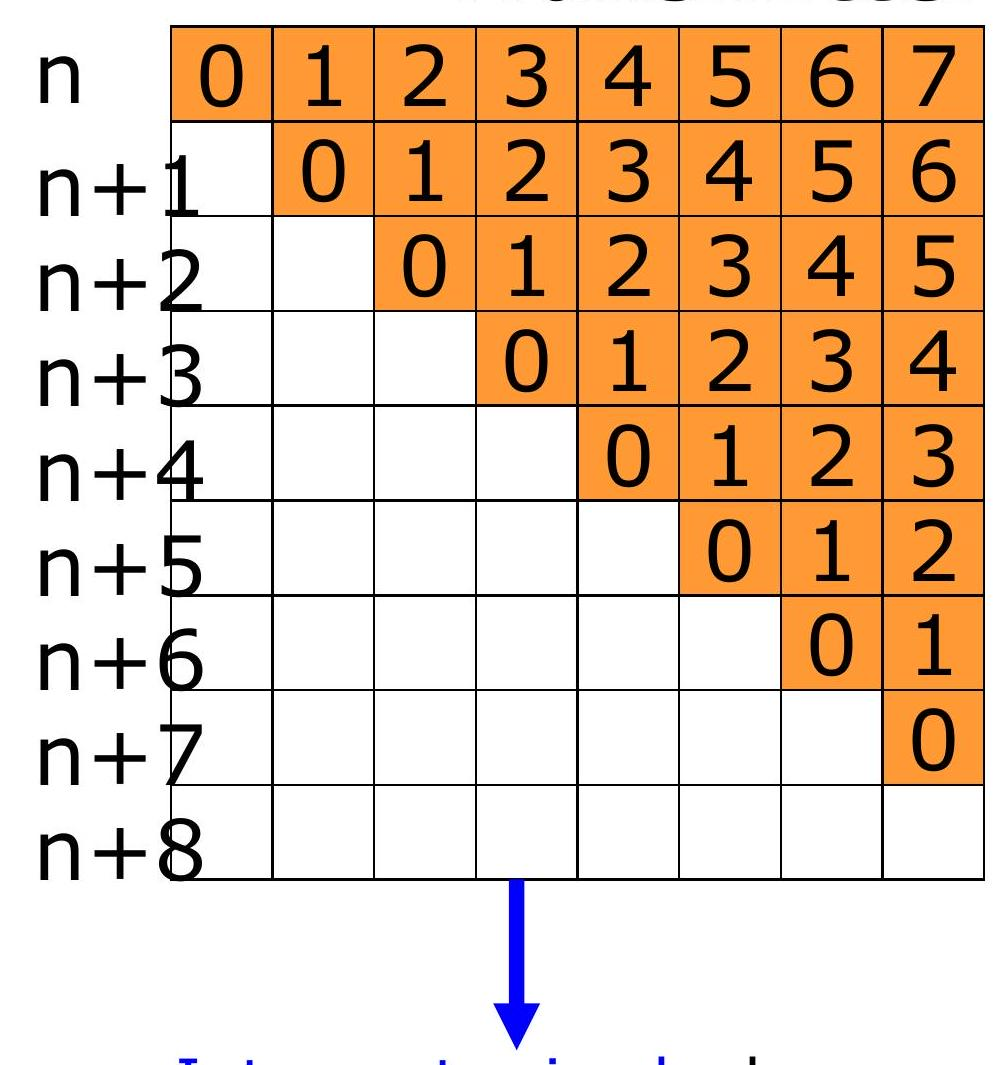
\includegraphics[max width=\textwidth]{2023_01_13_b07e3b4bcffdaab9792bg-210}
\end{center}

Interrupt raised when Transmitter $(T x)$ is empty $\Rightarrow$ Byte has been transmitted and next byte ready for loading

\begin{center}
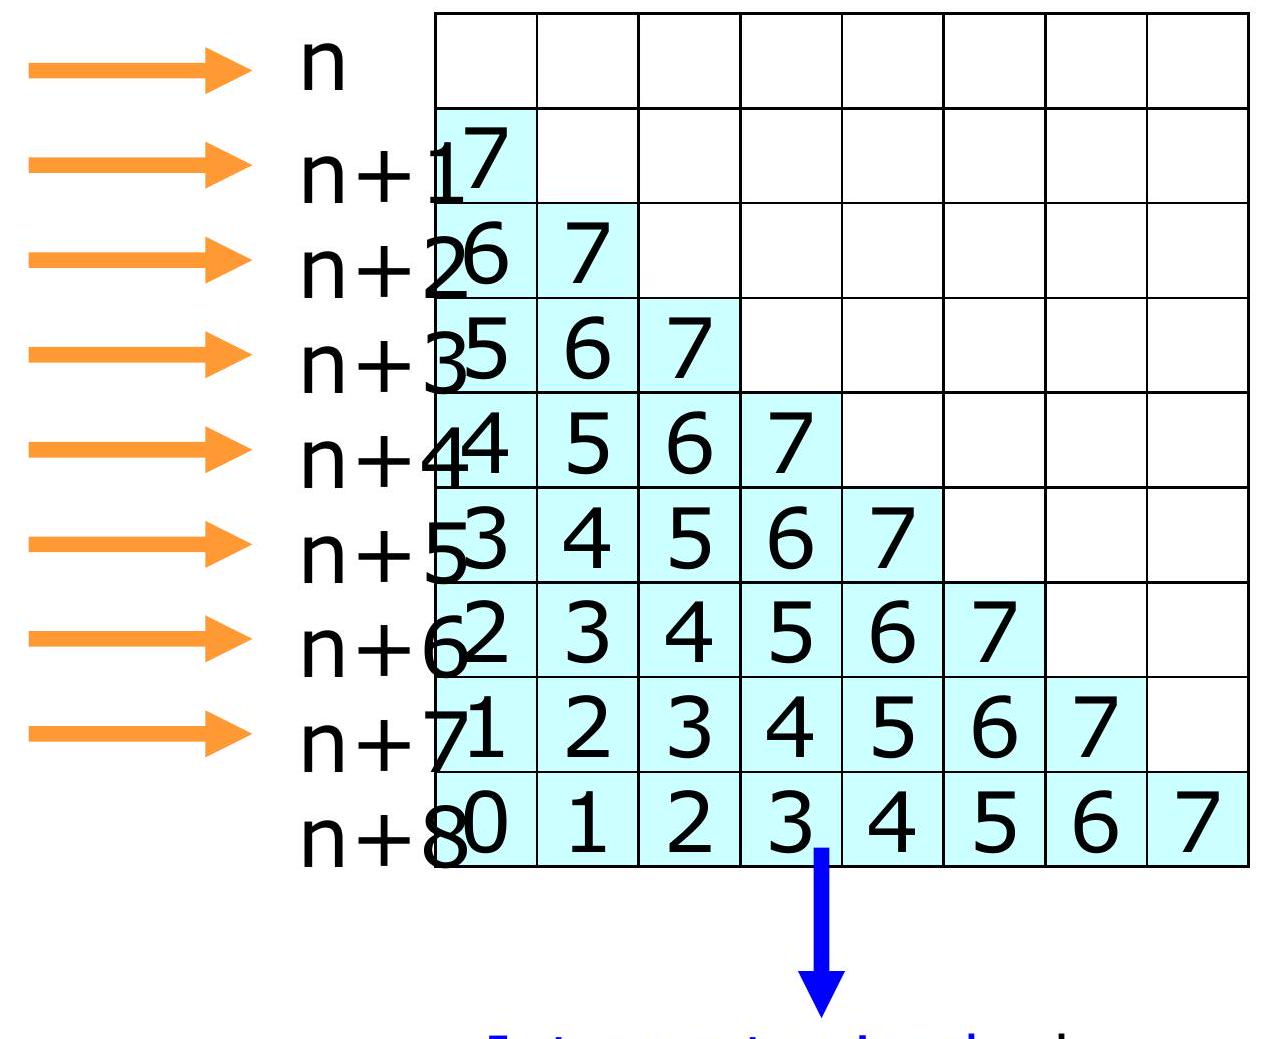
\includegraphics[max width=\textwidth]{2023_01_13_b07e3b4bcffdaab9792bg-210(1)}
\end{center}

Interrupt raised when Receiver $(R x)$ is full $\Rightarrow$ Byte has been received and is ready for reading


\os{newpage} item[{\rot\bf  Serial Bus Interface Motivations }]~\\[-3ex]

\bi
  \ite Motivation
\ei
\bi
 \ite Without using a lot of I/O lines
 \ei


$\times \mathrm{I} / \mathrm{O}$ lines require $\mathrm{I} / \mathrm{O}$ pads which cost $\$ \$ \$$ and size

\bi
  \ite I/O lines require PCB area which costs $\$ \$ \$$ and size
\ei
\bi
 \ite Connect different systems together
 \ei


\bi
  \ite Two embedded systems
\ei

$\times$ A desktop and an embedded system
\bi
 \ite Connect different chips together in the same embedded system
 \ei


\bi
  \ite MCU to peripheral
\ei

$\times \mathrm{MCU}$ to $\mathrm{MCU}$
\bi
 \ite Often at relatively low data rates
 \ei


\bi
  \ite But sometimes at higher data rates

  \ite So, what are our options?

\ei
\bi
 \ite Universal Synchronous/Asynchronous Receiver Transmitter
 \ei


\bi
  \ite Also known as USART (pronounced: "you-sart")
\ei


\os{newpage} item[{\rot\bf  Serial Bus Design Space }]~\\[-3ex]

\bi
  \ite Number of wires required?

  \ite Asynchronous or synchronous?

  \ite How fast can it transfer data?

  \ite Can it support more than two endpoints?

  \ite Can it support more than one master (i.e. txn initiator)?

  \ite How do we support flow control?

  \ite How does it handle errors/noise?

  \ite How far can signals travel?

\ei


\os{newpage} item[{\rot\bf  Serial Bus Examples }]~\\[-3ex]

\begin{center}
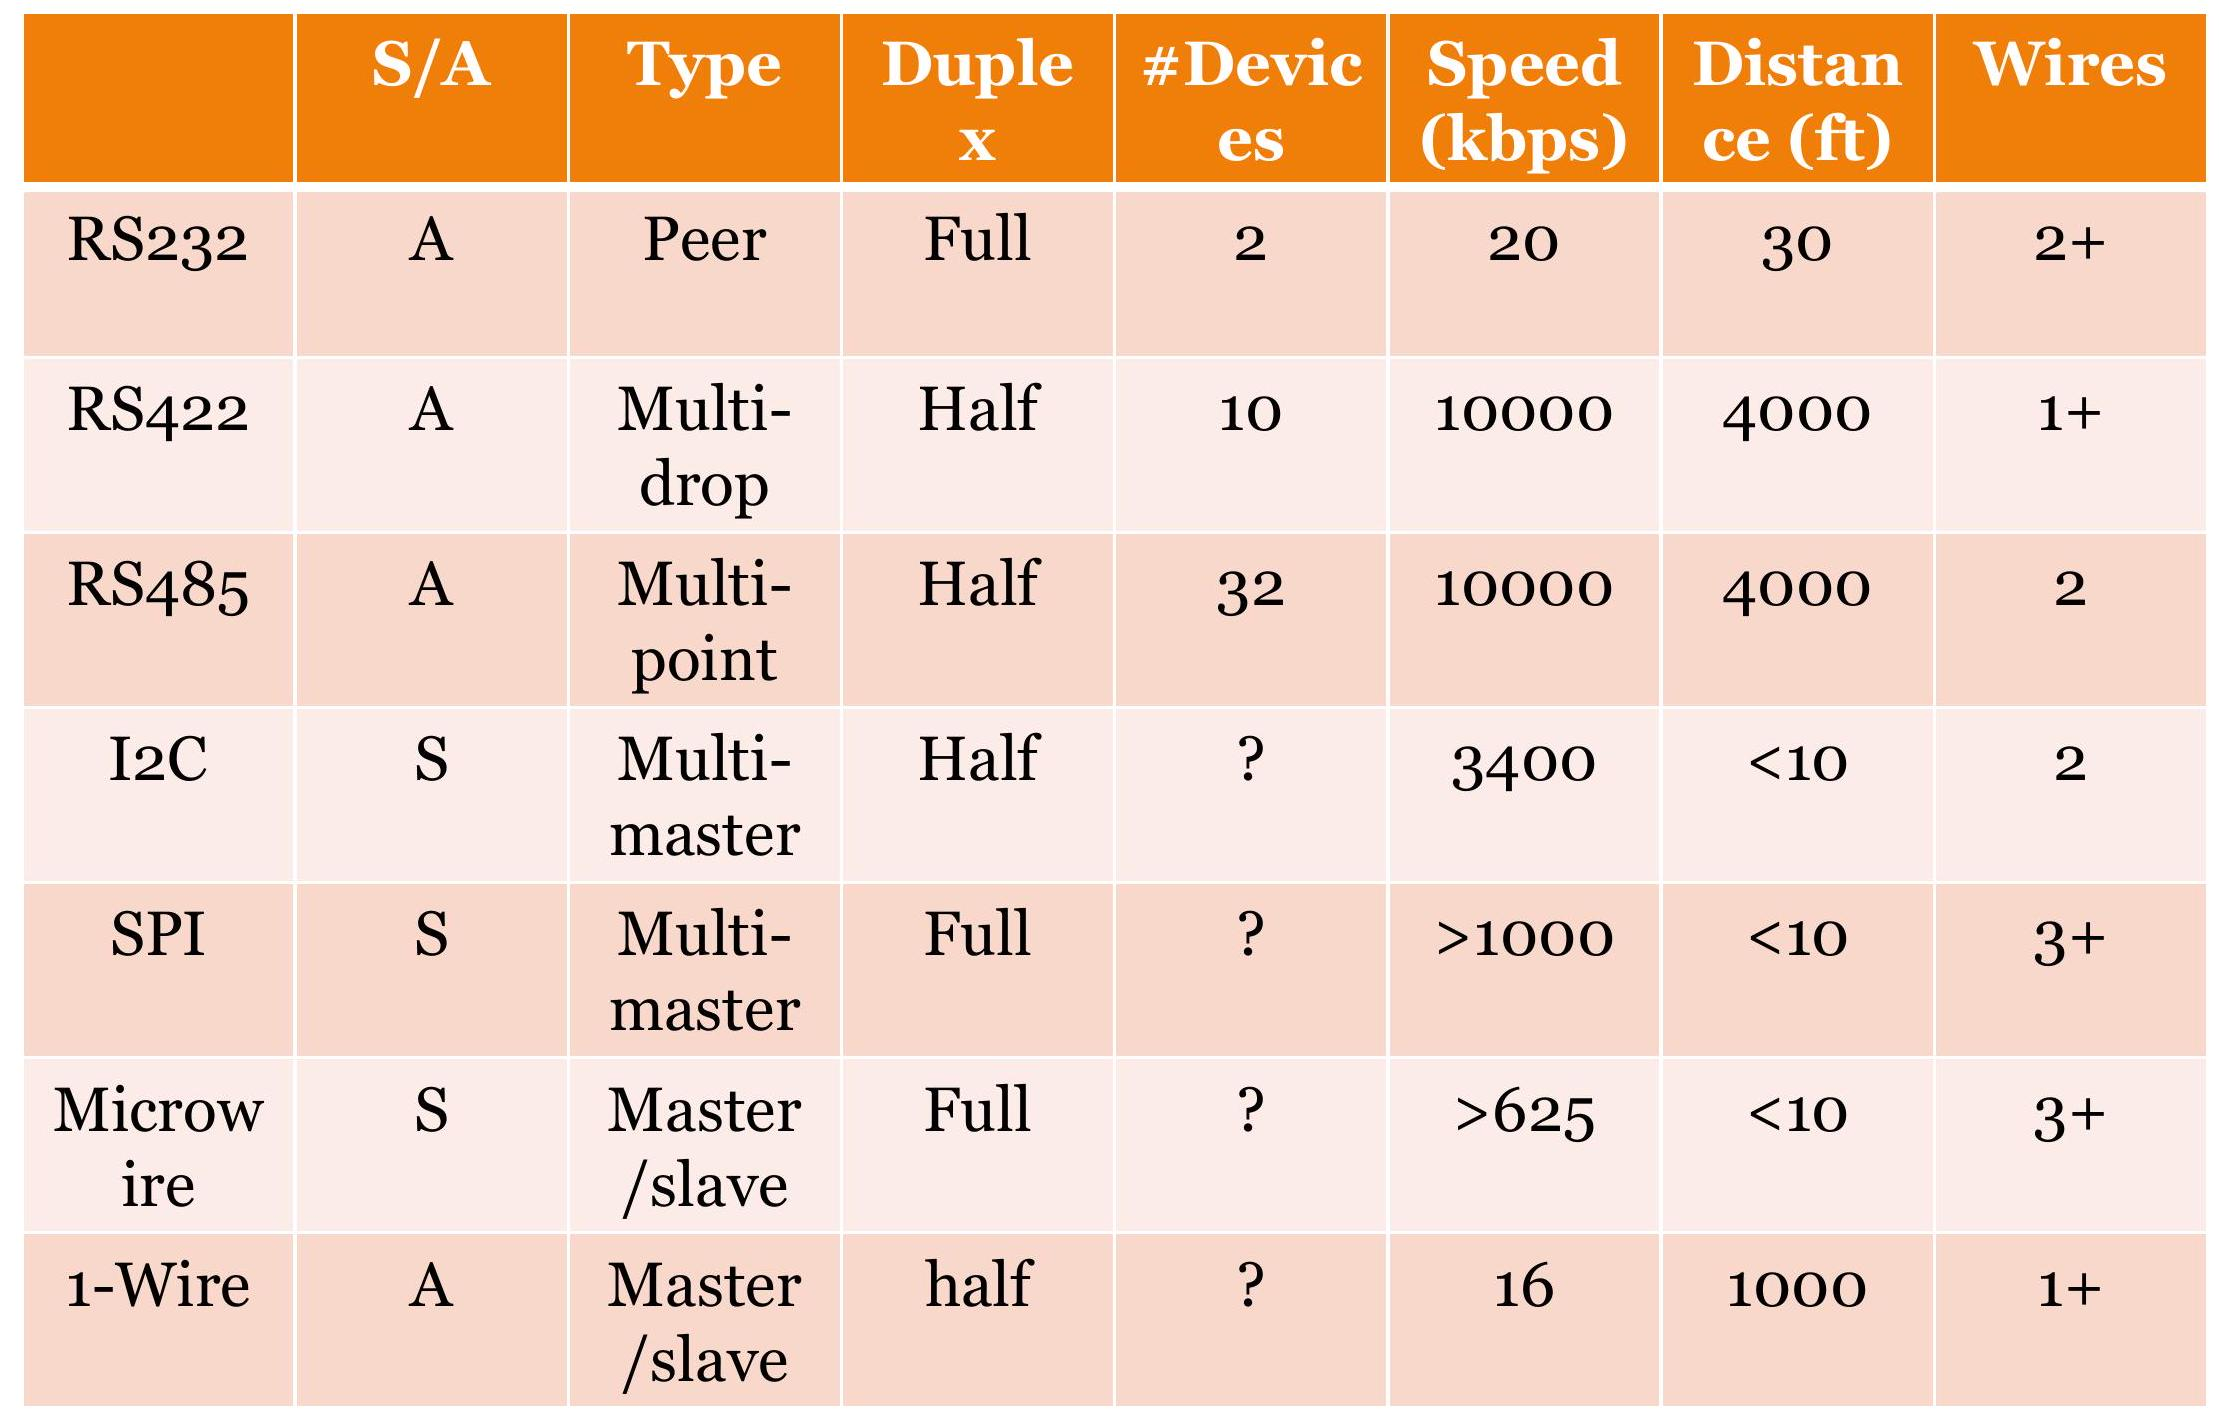
\includegraphics[max width=\textwidth]{2023_01_13_b07e3b4bcffdaab9792bg-213}
\end{center}


\os{newpage} item[{\rot\bf  UART Uses }]~\\[-3ex]

\bi
  \ite PC serial port is a UART!

  \ite Serializes data to be sent over serial cable - De-serializes received data
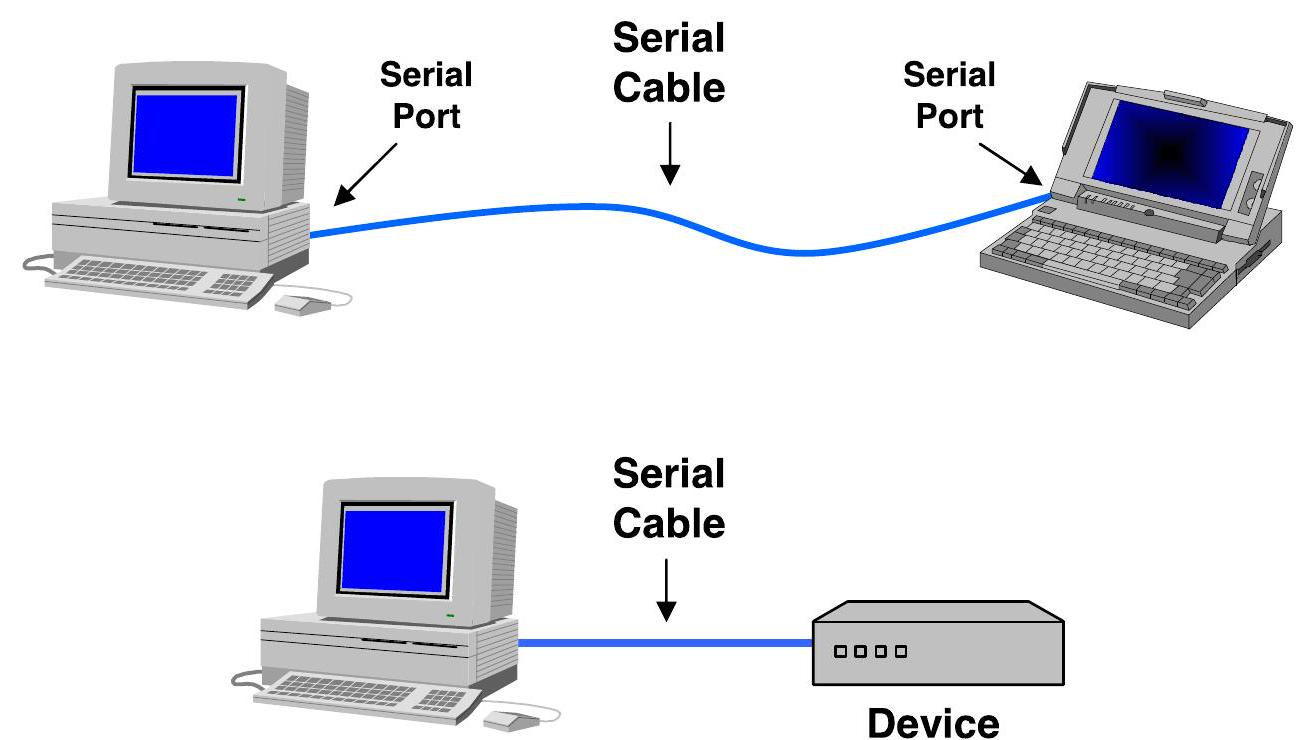
\includegraphics[max width=\textwidth, center]{2023_01_13_b07e3b4bcffdaab9792bg-214}

\ei


\os{newpage} item[{\rot\bf  UART Uses }]~\\[-3ex]


\os{newpage} item[{\rot\bf  - Used to be commonly used for internet access }]~\\[-3ex]

\begin{center}
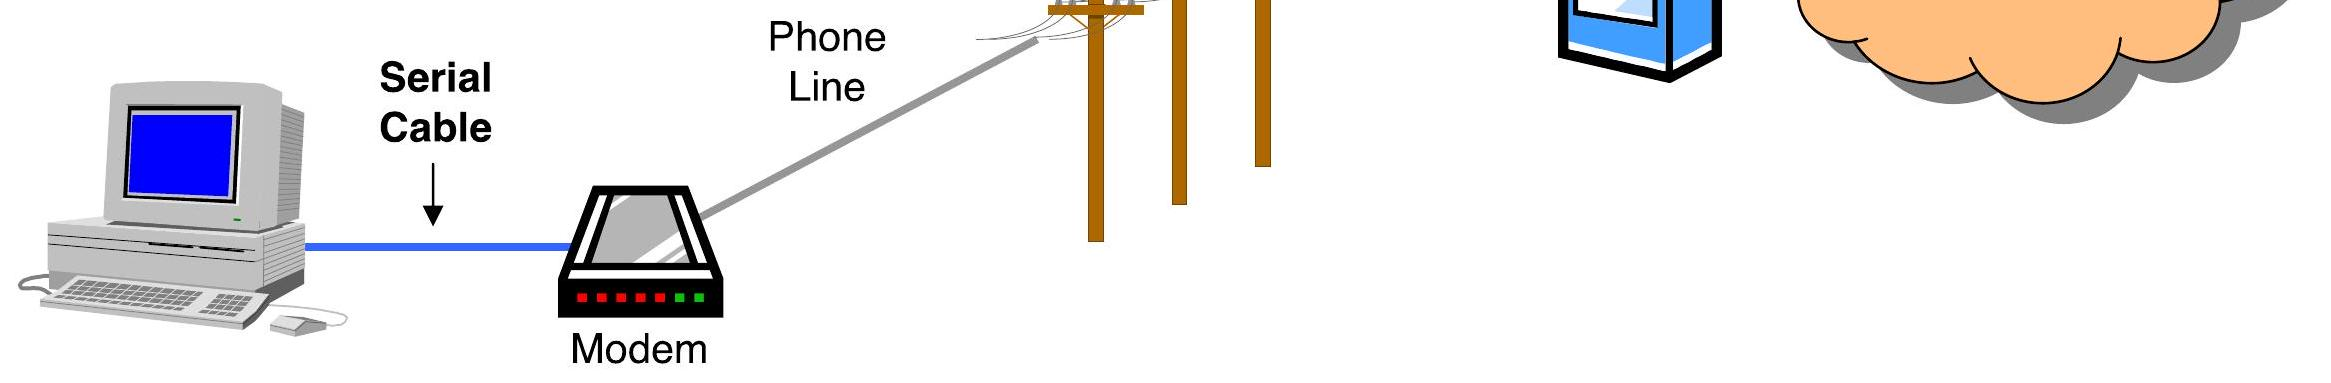
\includegraphics[max width=\textwidth]{2023_01_13_b07e3b4bcffdaab9792bg-215}
\end{center}


\os{newpage} item[{\rot\bf  UART }]~\\[-3ex]

\bi
  \ite Universal Asynchronous Receiver/Transmitter

  \ite Hardware that translates between parallel and serial forms

\ei


\os{newpage} item[{\rot\bf  - Commonly used in conjunction with communication standards such as EIA, RS-232, RS-422 or RS-485 }]~\\[-3ex]

\begin{center}
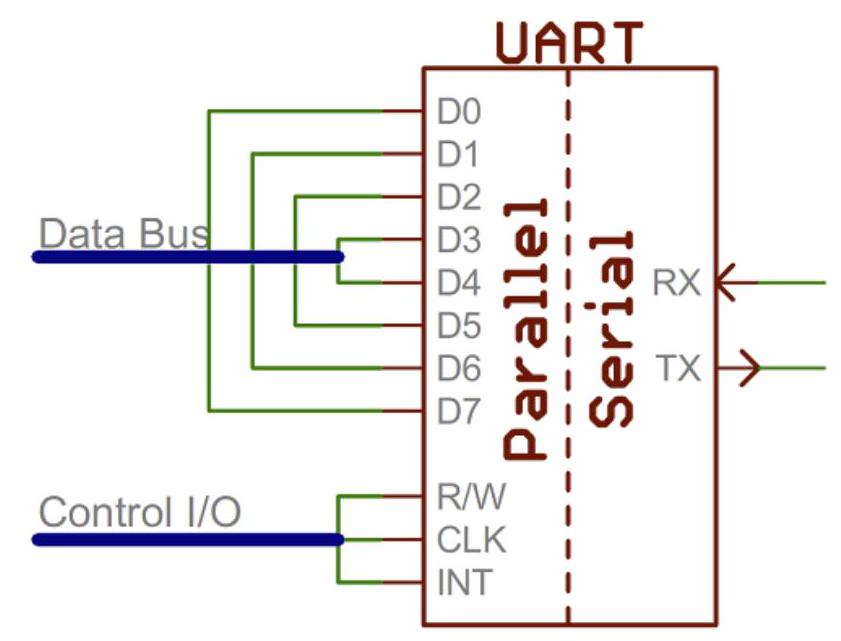
\includegraphics[max width=\textwidth]{2023_01_13_b07e3b4bcffdaab9792bg-216}
\end{center}


\os{newpage} item[{\rot\bf  Protocol }]~\\[-3ex]

\bi
  \ite Each character is sent as
\ei
\bi
 \ite a logic low start bit
 \ei

\bi
 \ite a configurable number of data bits (usually 7 or 8 , sometimes
 \ei


5.
\bi
 \ite an optional parity bit
 \ei

\bi
 \ite one or more logic high stop bits
 \ei

\bi
 \ite with a particular bit timing ("baud")
 \ei


\begin{center}
\begin{tabular}{|c|c|c|c|c|c|c|c|c|c|}
\hline
Start & Data 0 & Data 1 & Data 2 & Data 3 & Data & Data & Data & Data \\
5 & 6 & 7 & Stop &  &  &  &  &  \\
\hline
\end{tabular}
\end{center}


\os{newpage} item[{\rot\bf  UART Example }]~\\[-3ex]


\os{newpage} item[{\rot\bf  - Send the ASCII letter 'W' (1010111) }]~\\[-3ex]

\begin{center}
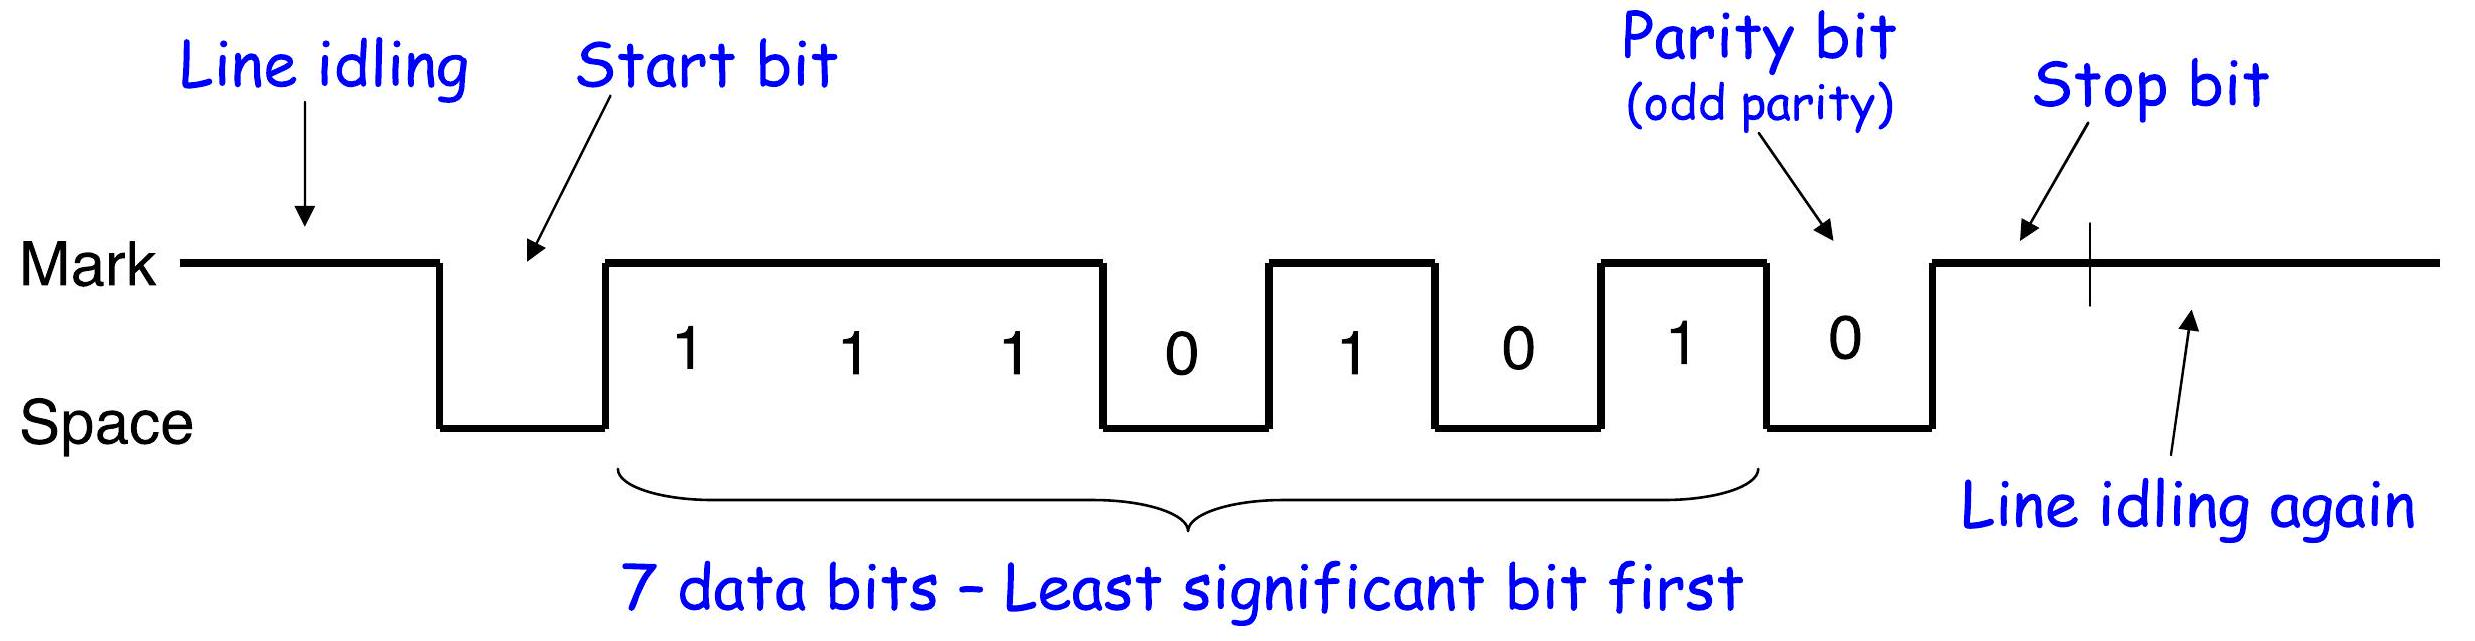
\includegraphics[max width=\textwidth]{2023_01_13_b07e3b4bcffdaab9792bg-218}
\end{center}


\os{newpage} item[{\rot\bf  UART Hardware Connection }]~\\[-3ex]

\begin{center}
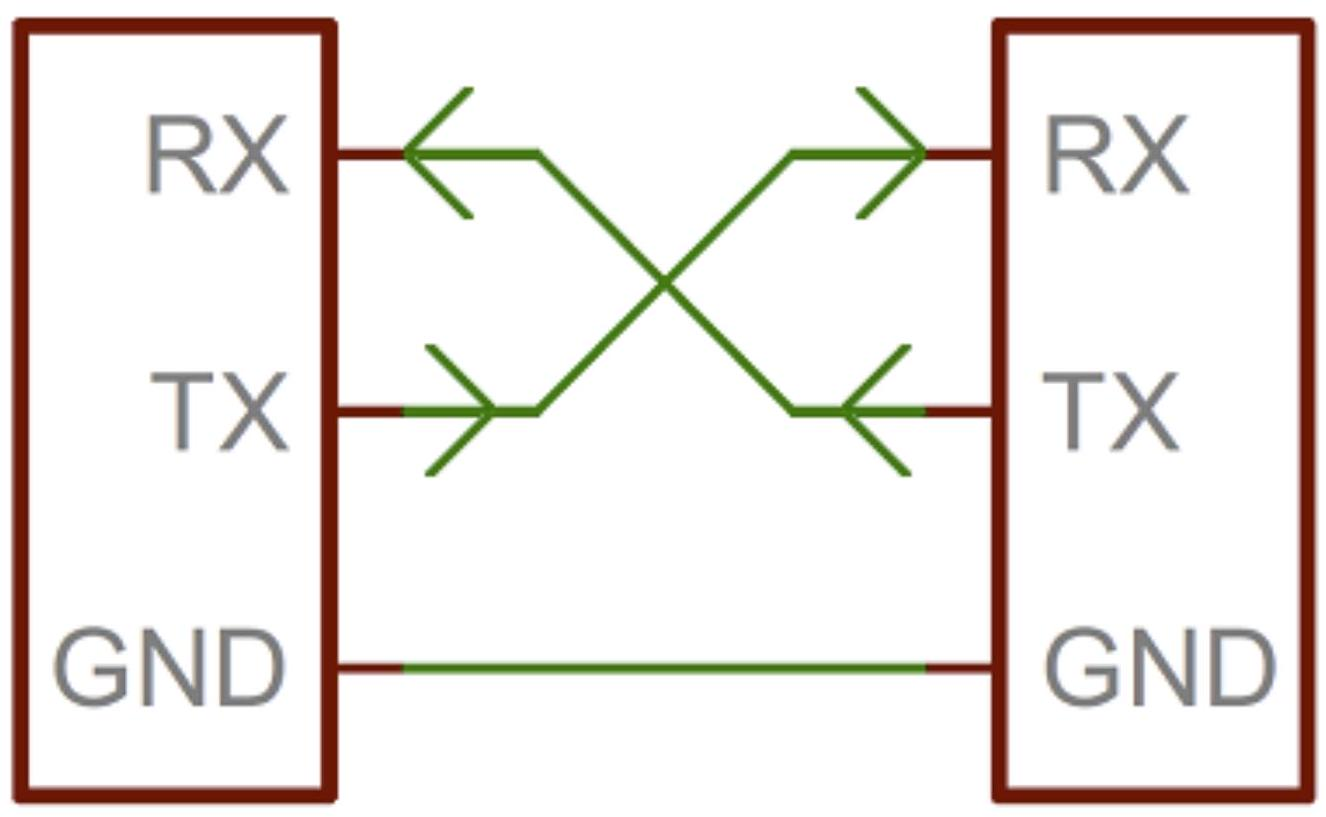
\includegraphics[max width=\textwidth]{2023_01_13_b07e3b4bcffdaab9792bg-219}
\end{center}


\os{newpage} item[{\rot\bf  UART Character Reception }]~\\[-3ex]

Start bit says a character is coming, receiver resets its timers

\begin{center}
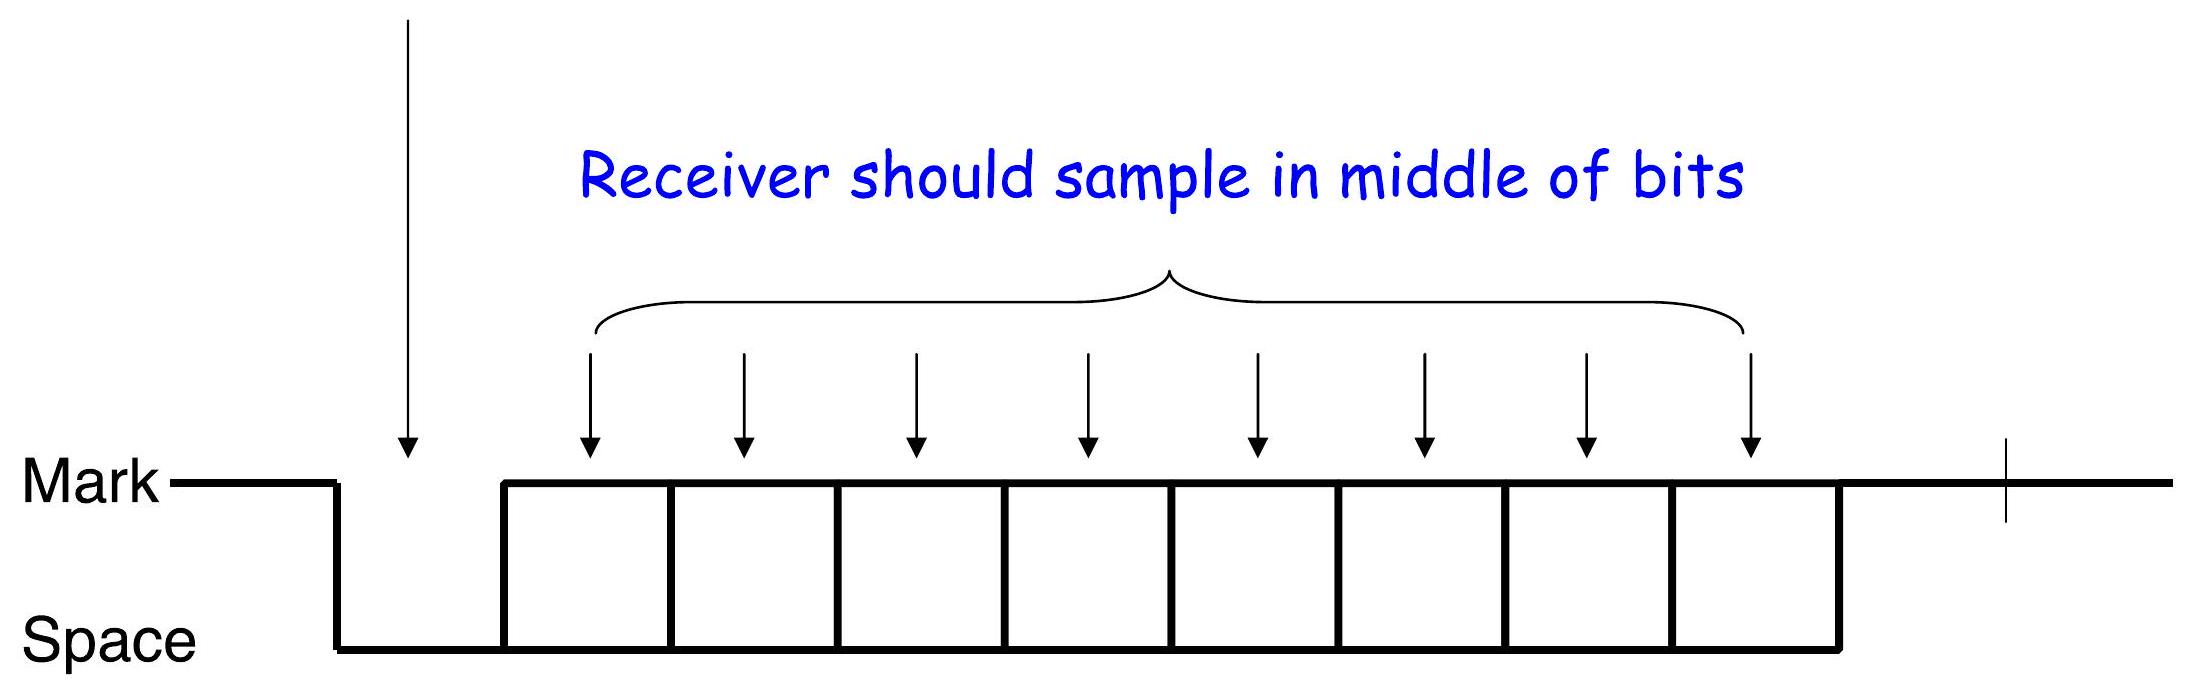
\includegraphics[max width=\textwidth]{2023_01_13_b07e3b4bcffdaab9792bg-220}
\end{center}

Receiver uses a timer (counter) to time when it samples.

Transmission rate (i.e., bit width) must be known!

Slides from BYU CS 224


\os{newpage} item[{\rot\bf  UART Character Reception }]~\\[-3ex]

If receiver samples too quickly, see what happens...

Space

\begin{center}
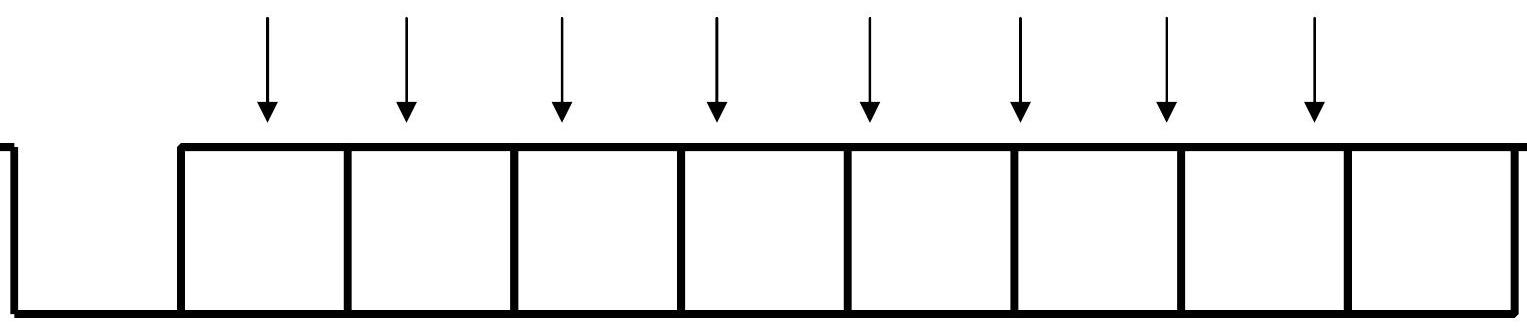
\includegraphics[max width=\textwidth]{2023_01_13_b07e3b4bcffdaab9792bg-221}
\end{center}


\os{newpage} item[{\rot\bf  UART Character Reception }]~\\[-3ex]

If receiver samples too slowly, see what happens...

Mark

Space

\begin{center}
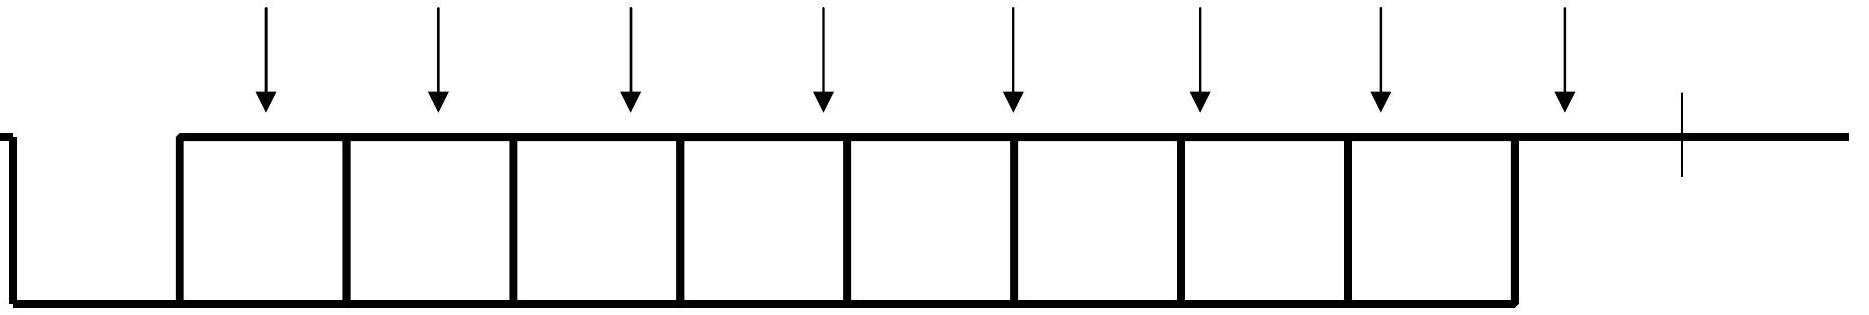
\includegraphics[max width=\textwidth]{2023_01_13_b07e3b4bcffdaab9792bg-222}
\end{center}

Receiver resynchronizes on every start bit. Only has to be accurate enough to read 9 bits.


\os{newpage} item[{\rot\bf  UART Character Reception }]~\\[-3ex]

\bi
  \ite Receiver also verifies that stop bit is ' 1 '

  \ite If not, reports "framing error" to host system

  \ite New start bit can appear immediately after stop bit - Receiver will resynchronize on each start bit

\ei


\os{newpage} item[{\rot\bf  Let us design a UART transmitter }]~\\[-3ex]

\begin{center}
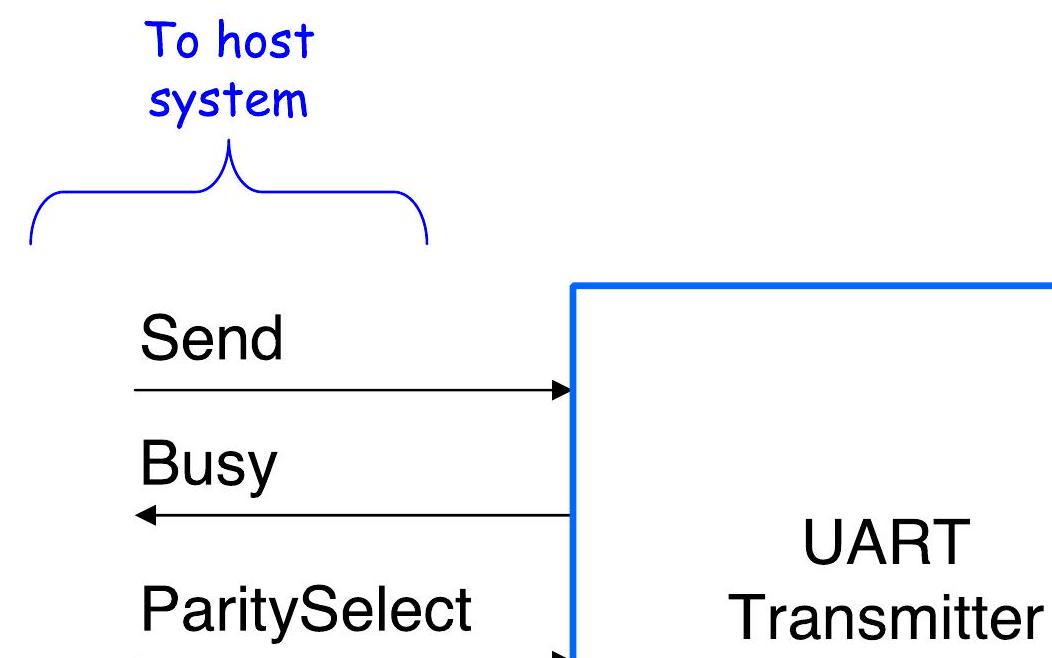
\includegraphics[max width=\textwidth]{2023_01_13_b07e3b4bcffdaab9792bg-224}
\end{center}


\os{newpage} item[{\rot\bf  Transmitter/System Handshaking }]~\\[-3ex]

\bi
  \ite System asserts Send and holds it high when it wants to send a byte

  \ite UART asserts Busy signal in response

  \ite When UART has finished transfer, UART de-asserts Busy signal

  \ite System de-asserts Send signal
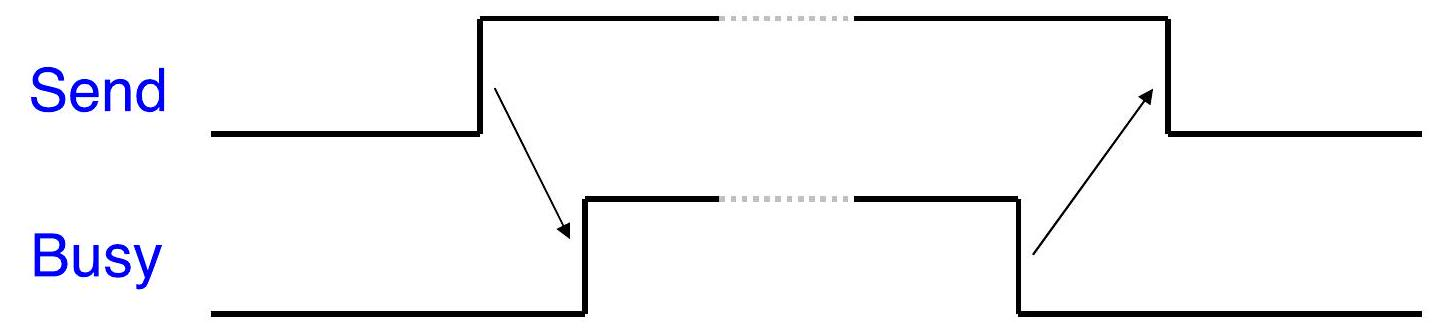
\includegraphics[max width=\textwidth, center]{2023_01_13_b07e3b4bcffdaab9792bg-225}

\ei


\os{newpage} item[{\rot\bf  Transmitter Block Diagram }]~\\[-3ex]

\begin{center}
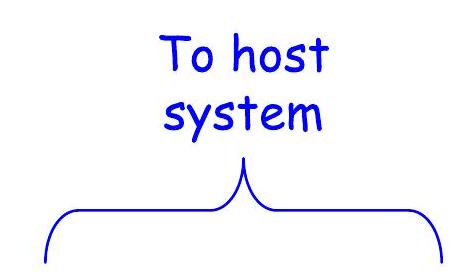
\includegraphics[max width=\textwidth]{2023_01_13_b07e3b4bcffdaab9792bg-226}
\end{center}

Send

\begin{center}
\begin{tabular}{l}
Busy \\
\hline
ParitySelect \\
\hline
\end{tabular}
\end{center}

ParitySelect

Din $300 \mathrm{HZ}$

Timer

Mod10

Counter State

Machine

Parity

Generator Shift

Register


\os{newpage} item[{\rot\bf  Discussion Questions }]~\\[-3ex]

\bi
  \ite How fast can we run a UART?

  \ite What are the limitations?

  \ite Why do we need start/stop bits?

  \ite How many data bits can be sent?

\ei

19200 baud rate, no parity, 8 data bits, 1 stop bit


\os{newpage} item[{\rot\bf  Serial Peripheral Interconnect (SPI) }]~\\[-3ex]

\bi
  \ite Another kind of serial protocol in embedded systems (proposed by Motorola)

  \ite Four-wire protocol o SCLK - Serial Clock

  \ite MOSI/SIMO - Master Output, Slave Input

  \ite MISO/SOMI - Master Input, Slave Output

  \ite SS - Slave Select

  \ite Single master device and with one or more slave devices

  \ite Higher throughput than I2C and can do "stream transfers"

  \ite No arbitration required

  \ite But

  \ite Requires more pins

  \ite Has no hardware flow control

  \ite No slave acknowledgment (master could be talking to thin air and not even know it)

\ei


\os{newpage} item[{\rot\bf  What is SPI? }]~\\[-3ex]

\bi
  \ite Serial Bus protocol

  \ite Fast, \href{http://Easy.to}{Easy.to} use, Simpleat ..... ° - Everyor'

\ei

\begin{center}
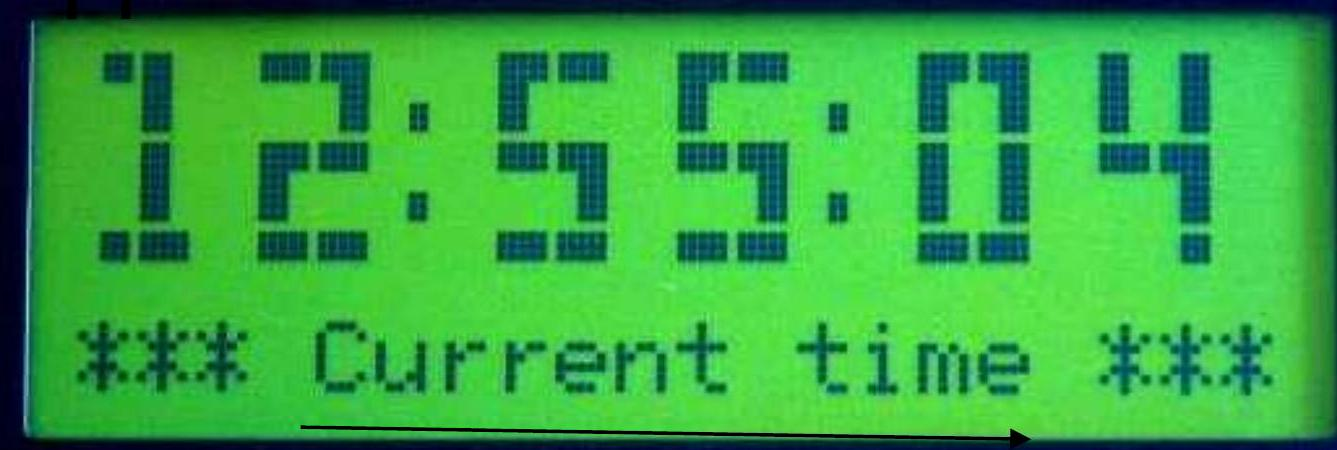
\includegraphics[max width=\textwidth]{2023_01_13_b07e3b4bcffdaab9792bg-229}
\end{center}

\begin{center}

\includegraphics[max width=\textwidth]{2023_01_13_b07e3b4bcffdaab9792bg-229(1)}
\end{center}

Digital Set-Top Box Integrated Controller

POWCNDET

75H6051 03BM 1F11DOORPB KOREA

\begin{center}
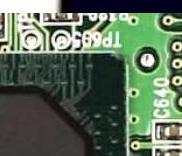
\includegraphics[max width=\textwidth]{2023_01_13_b07e3b4bcffdaab9792bg-229(2)}
\end{center}

IBM39 STB02100 PBC 22C




\os{newpage} item[{\rot\bf  SPI Basics }]~\\[-3ex]


\os{newpage} item[{\rot\bf  - A communication protocol using 4 wires Also known as a 4 wire bus }]~\\[-3ex]


\os{newpage} item[{\rot\bf  - Used to communicate across small distances }]~\\[-3ex]


\os{newpage} item[{\rot\bf  - Multiple Slaves, Single Master }]~\\[-3ex]


\os{newpage} item[{\rot\bf  - Synchronized }]~\\[-3ex]


\os{newpage} item[{\rot\bf  SPI Capabilities }]~\\[-3ex]

\bi
  \ite Always Full Duplex

  \ite Communicating in two directions at the same time

  \ite Transmission need not be meaningful

  \ite Multiple Mbps transmission speed

\ei


\os{newpage} item[{\rot\bf  - Transfers data in 4 to 16 bit characters }]~\\[-3ex]

\bi
  \ite Multiple slaves

  \ite Daisy-chaining possible

\ei


\os{newpage} item[{\rot\bf  SPI Protocol }]~\\[-3ex]

\bi
  \ite Wires:
\ei
\bi
 \ite Master Out Slave In (MOSI)
 \ei

\bi
 \ite Master In Slave Out (MISO)
 \ei

\bi
 \ite System Clock (SCLK)
 \ei


\bi
  \ite Slave Select 1...N
\ei

\begin{center}
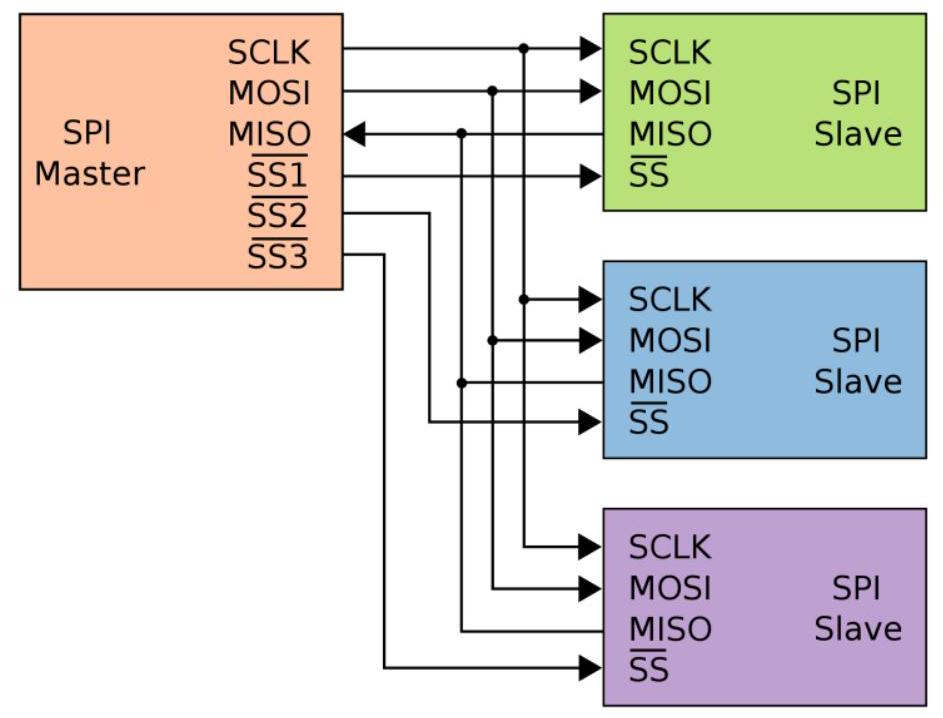
\includegraphics[max width=\textwidth]{2023_01_13_b07e3b4bcffdaab9792bg-232}
\end{center}

\bi
  \ite Master Generates Clock

  \ite Master Set Slave Select low

  \ite Shift registers shift in and out data

\ei


\os{newpage} item[{\rot\bf  SPI Wires in Detail }]~\\[-3ex]


\os{newpage} item[{\rot\bf  - MOSI - Carries data out of Master to Slave }]~\\[-3ex]

\bi
  \ite MISO - Carries data from Slave to Master - Both signals happen for every transmission

  \ite SS\_BAR - Unique line to select a slave

\ei


\os{newpage} item[{\rot\bf  - SCLK - Master produced clock to synchronize data transfer }]~\\[-3ex]

\begin{center}
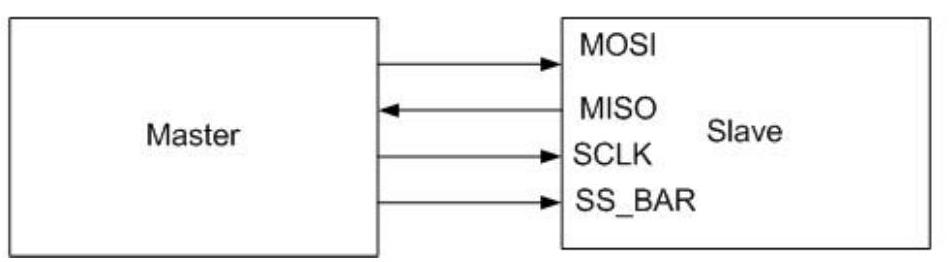
\includegraphics[max width=\textwidth]{2023_01_13_b07e3b4bcffdaab9792bg-233}
\end{center}


\os{newpage} item[{\rot\bf  SPI uses a "shift register" model of communications }]~\\[-3ex]


\os{newpage} item[{\rot\bf  Master }]~\\[-3ex]

Slave

\begin{center}
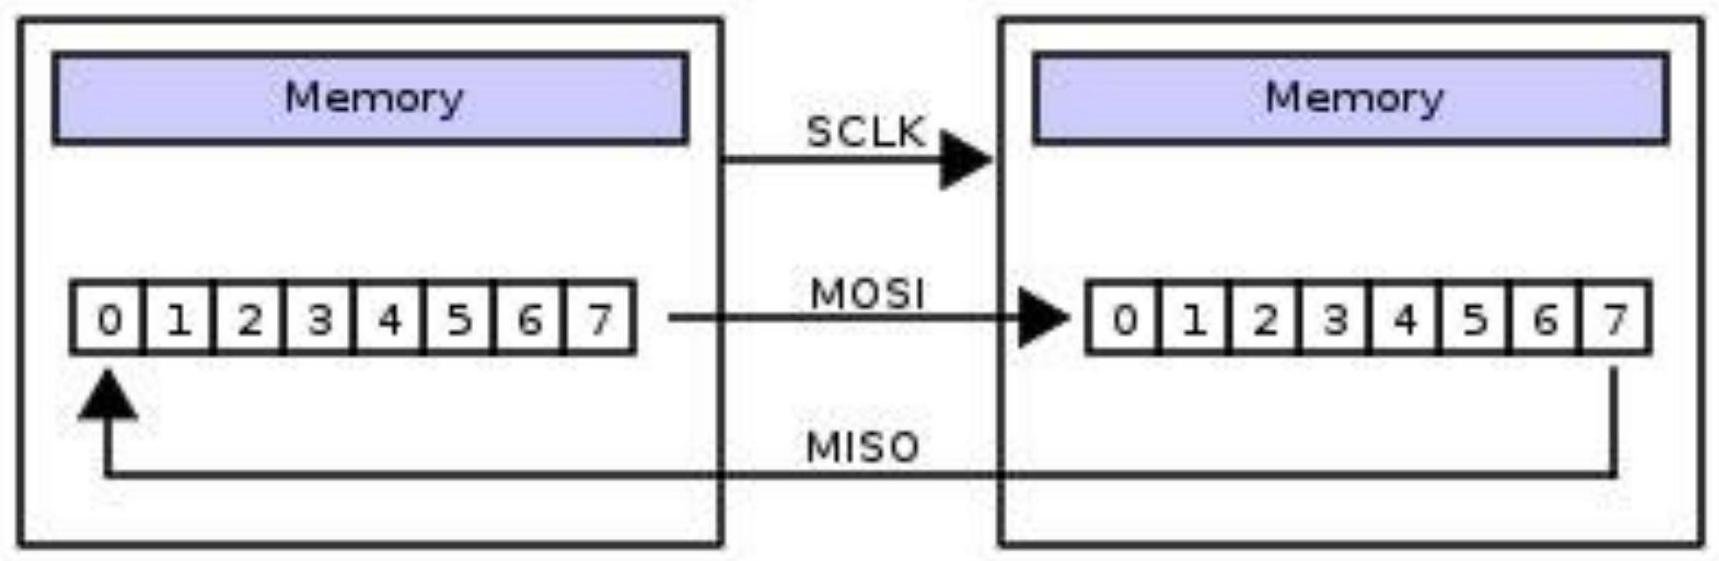
\includegraphics[max width=\textwidth]{2023_01_13_b07e3b4bcffdaab9792bg-234}
\end{center}

Master shifts out data to Slave, and shifts in data from Slave \href{http://upload.wikimedia.org/wikipedia/commons/thumb/b/bb/SPI_8-bit_circular_transfer.svg/400px-SPI_8-bit_circular_transfer.svg.png}{http://upload.wikimedia.org/wikipedia/commons/thumb/b/bb/SPI\_8-bit\_circular\_transfer.svg/400px-SPI\_8-bit\_circular\_transfer.svg.png}


\os{newpage} item[{\rot\bf  SPI Communication }]~\\[-3ex]

\begin{center}
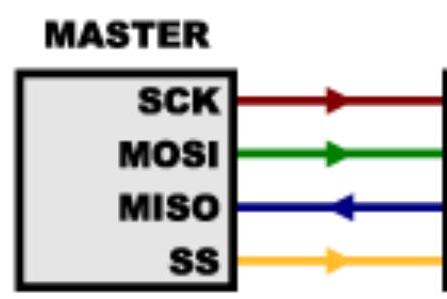
\includegraphics[max width=\textwidth]{2023_01_13_b07e3b4bcffdaab9792bg-235}
\end{center}

SLAVE

SCK

MosI

MISO

Ss

\begin{center}
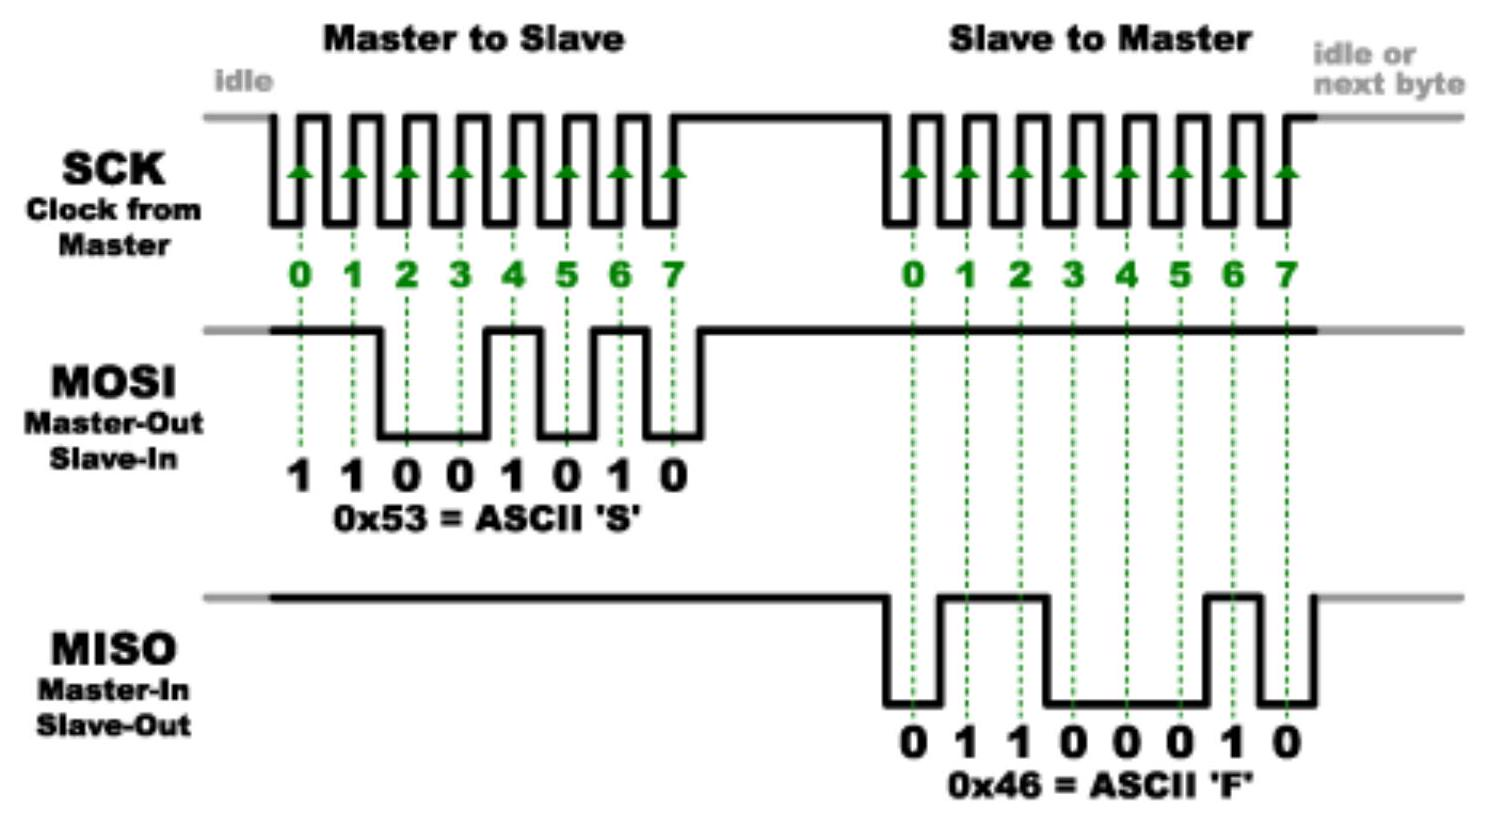
\includegraphics[max width=\textwidth]{2023_01_13_b07e3b4bcffdaab9792bg-235(1)}
\end{center}

\begin{center}
\begin{tabular}{c|l|l}
SS \\
Slave-Select \\
\end{tabular}
\end{center}


\os{newpage} item[{\rot\bf  SPI clocking: there is no "standard way" }]~\\[-3ex]

\bi
  \ite Four clocking “modes"

  \ite Two phases

  \ite Two polarities

  \ite Master and selected slave must be in the same mode

  \ite During transfers with slaves A and B, Master must

  \ite Configure clock to Slave A's clock mode

  \ite Select Slave A

  \ite Do transfer

  \ite Deselect Slave A

  \ite Configure clock to Slave B's clock mode

  \ite Select Slave B

  \ite Do transfer

  \ite Deselect Slave B

  \ite Master reconfigures clock mode on-the-fly!

\ei


\os{newpage} item[{\rot\bf  SPI timing diagram }]~\\[-3ex]

\begin{center}
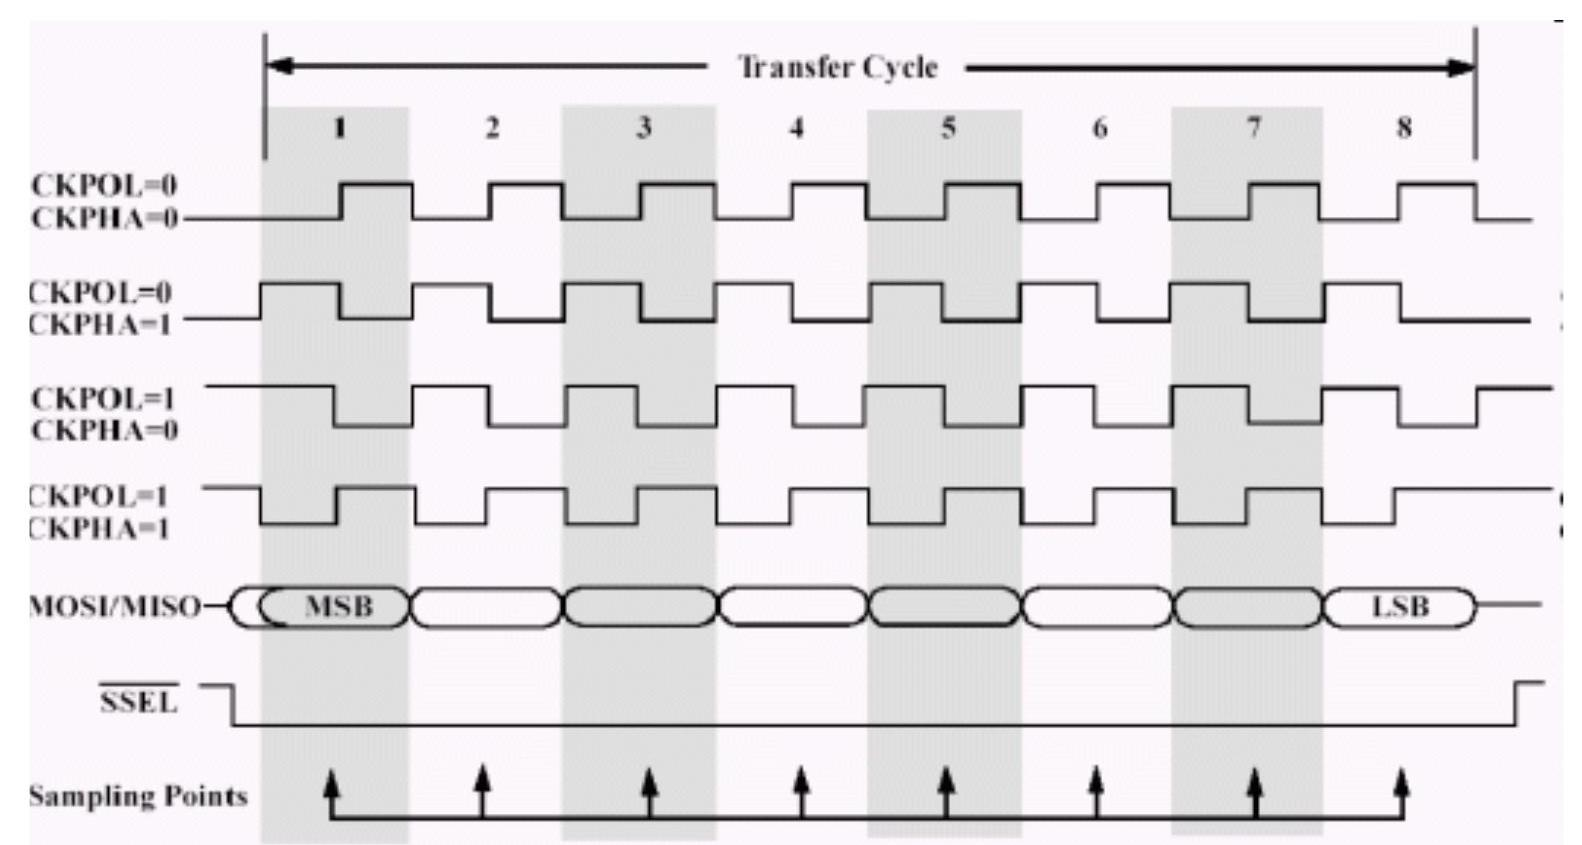
\includegraphics[max width=\textwidth]{2023_01_13_b07e3b4bcffdaab9792bg-237}
\end{center}

Timing Diagram - Showing Clock polarities and phases \href{http://www.maxim-ic.com.cn/images/appnotes/3078/3078Fig02.gif}{http://www.maxim-ic.com.cn/images/appnotes/3078/3078Fig02.gif}


\os{newpage} item[{\rot\bf  SPI Pros and Cons }]~\\[-3ex]

\bi
  \ite Pros:

  \ite Fast and easy
Fast for point-to-point connections

Easily allows streaming/Constant data inflow

No addressing/Simple to implement

Everyone supports it

  \ite Cons:

\ei

SS makes multiple slaves very complicated

\bi
  \ite No acknowledgement ability

  \ite No inherent arbitration

\ei

No flow control


\os{newpage} item[{\rot\bf  I2C bus in our projects }]~\\[-3ex]

\bi
  \ite Communication with the accelerometer
\ei

Read from the accelerometer

\bi
  \ite Pros

  \ite Simple wire connection

  \ite Two wires bus that can connect multiple peripherals with the $\mathrm{MCU}$

  \ite Cons

  \ite Complexity is significantly higher

\ei


\os{newpage} item[{\rot\bf  How to operate the camera? }]~\\[-3ex]

Accel

\begin{center}
\begin{tabular}{|l|l|l|}
\hline
MCU \\
\hline
\end{tabular}
\end{center}

\href{https://www.youtube.com/watch?v}{https://www.youtube.com/watch?v} $=e q Z g$

xR6eRjo


\os{newpage} item[{\rot\bf  I2C Details }]~\\[-3ex]

\bi
  \ite Two lines
\ei
\bi
 \ite Serial data line (SDA)
 \ei

\bi
 \ite Serial clock line (SCL)
 \ei



\os{newpage} item[{\rot\bf  - Only two wires for connecting multiple devices }]~\\[-3ex]

\begin{center}
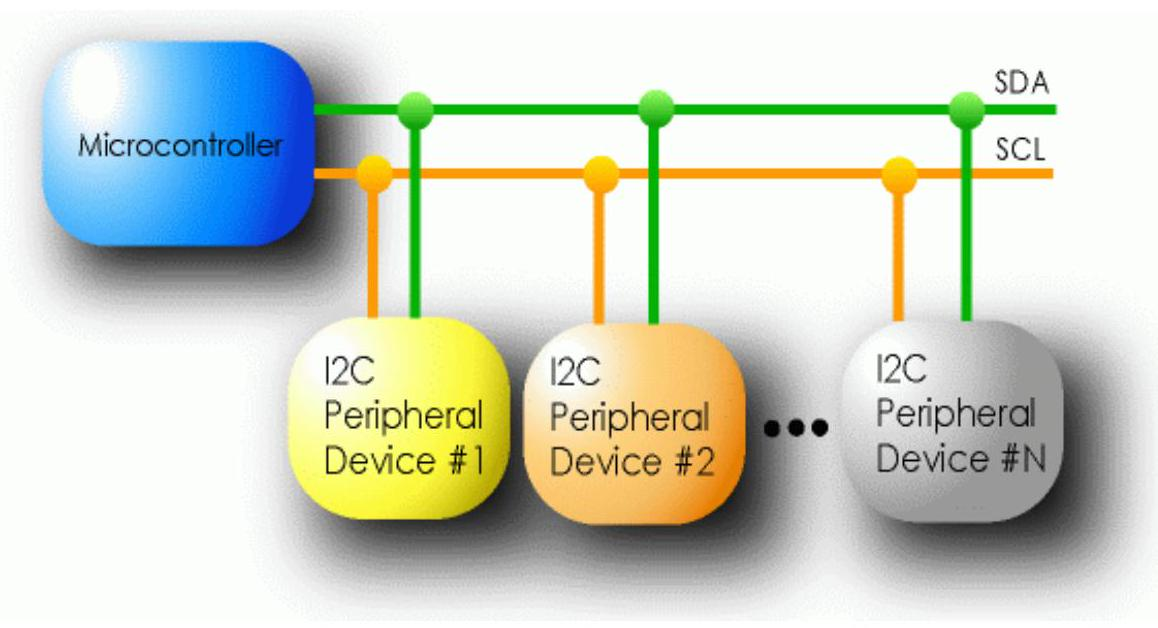
\includegraphics[max width=\textwidth]{2023_01_13_b07e3b4bcffdaab9792bg-241}
\end{center}


\os{newpage} item[{\rot\bf  I2C Details }]~\\[-3ex]


\os{newpage} item[{\rot\bf  - Each I2C device recognized by a unique address }]~\\[-3ex]


\os{newpage} item[{\rot\bf  - Each I2C device can be either a transmitter or receiver }]~\\[-3ex]


\os{newpage} item[{\rot\bf  - I2C devices can be masters or slaves for a data transfer }]~\\[-3ex]
\bi
 \ite Master (usually a microcontroller): Initiates a data transfer on the bus, generates the clock signals to permit that transfer, and terminates the transfer
 \ei

\bi
 \ite Slave: Any device addressed by the master at that time
 \ei



\os{newpage} item[{\rot\bf  Bit Transfer on the $\mathrm{I}^{2} \mathrm{C}$ Bus }]~\\[-3ex]

\bi
  \ite In normal data transfer, the data line only changes state when the clock is low
\ei

$\mathrm{SCL}$ SDA

$\mathrm{SCL}$

\begin{center}
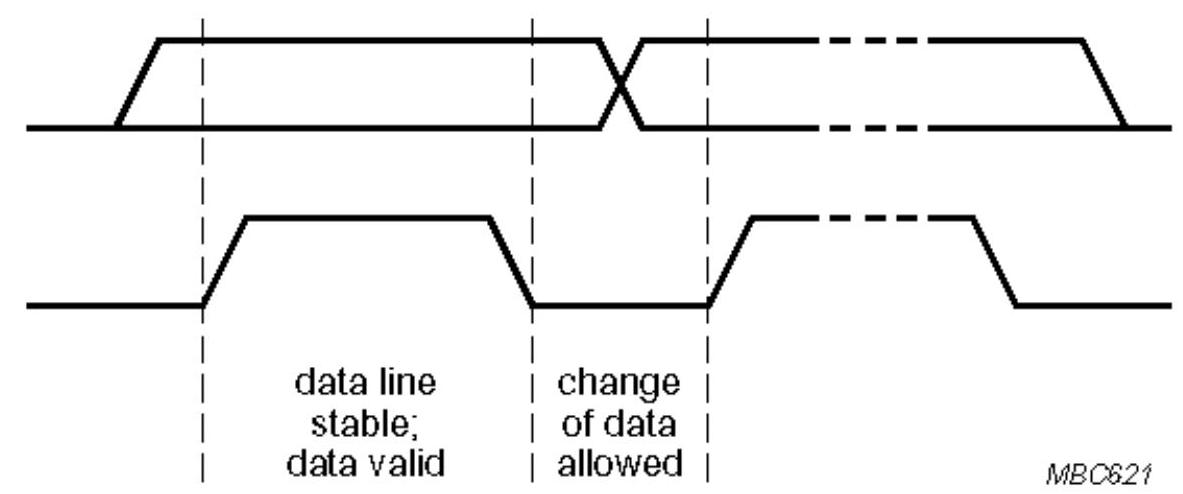
\includegraphics[max width=\textwidth]{2023_01_13_b07e3b4bcffdaab9792bg-243}
\end{center}

Data line stable; Data valid

\begin{center}

\includegraphics[max width=\textwidth]{2023_01_13_b07e3b4bcffdaab9792bg-243(1)}
\end{center}

$\mathrm{d}$


\os{newpage} item[{\rot\bf  Start and Stop Conditions }]~\\[-3ex]

A transition of the data line while the clock line is high is defined as either a start or a stop condition.

Both start and stop conditions are generated by the bus master

The bus is considered busy after a start condition, until a stop condition occurs

\begin{center}
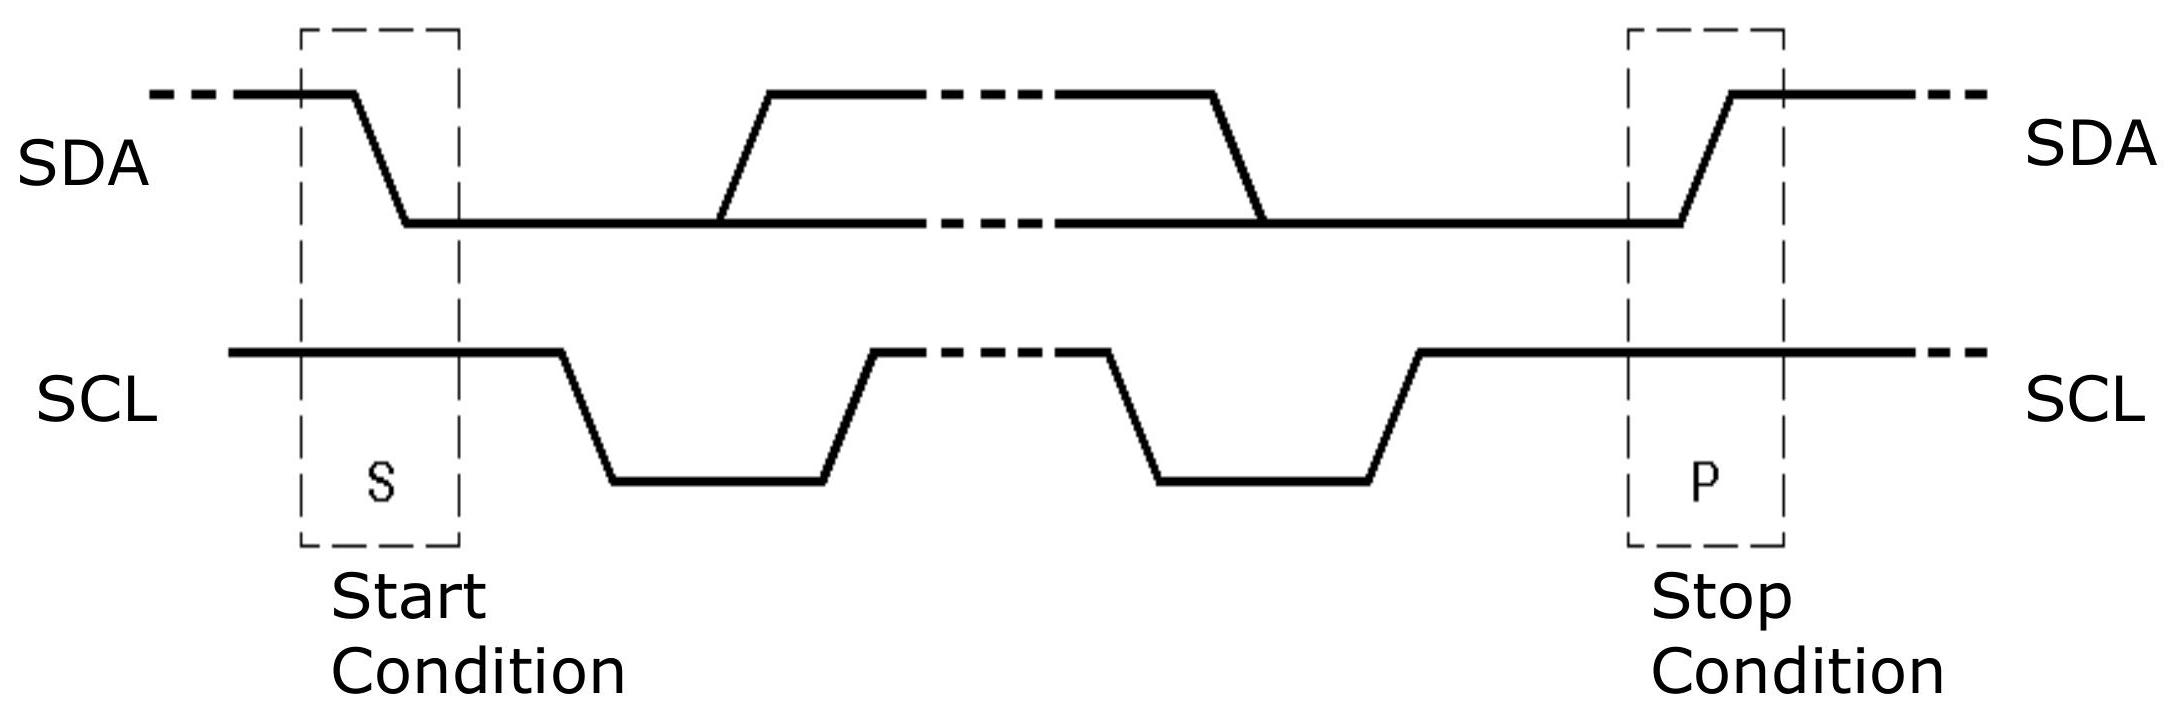
\includegraphics[max width=\textwidth]{2023_01_13_b07e3b4bcffdaab9792bg-244}
\end{center}


\item[{\rot\bf  $\mathrm{I}^{2} \mathrm{C}$ Addressing  }]~\\[-3ex]


\os{newpage} item[{\rot\bf  - Each node has a unique 7 (or 10) bit address }]~\\[-3ex]


\os{newpage} item[{\rot\bf  - Peripherals often have fixed and programmable address portions }]~\\[-3ex]


\os{newpage} item[{\rot\bf  - Addresses starting with o000 or 1111 have special functions:- }]~\\[-3ex]


\bi
  \ite 0000000 Is a General Call Address \textbackslash  o o000001 Is a Null (CBUS) Address \textbackslash  o 1111XXX Address Extension \textbackslash  O 1111111 Address Extension - Next Bytes are the Actual Address
\ei


\os{newpage} item[{\rot\bf  I2C-Connected System }]~\\[-3ex]

\begin{center}
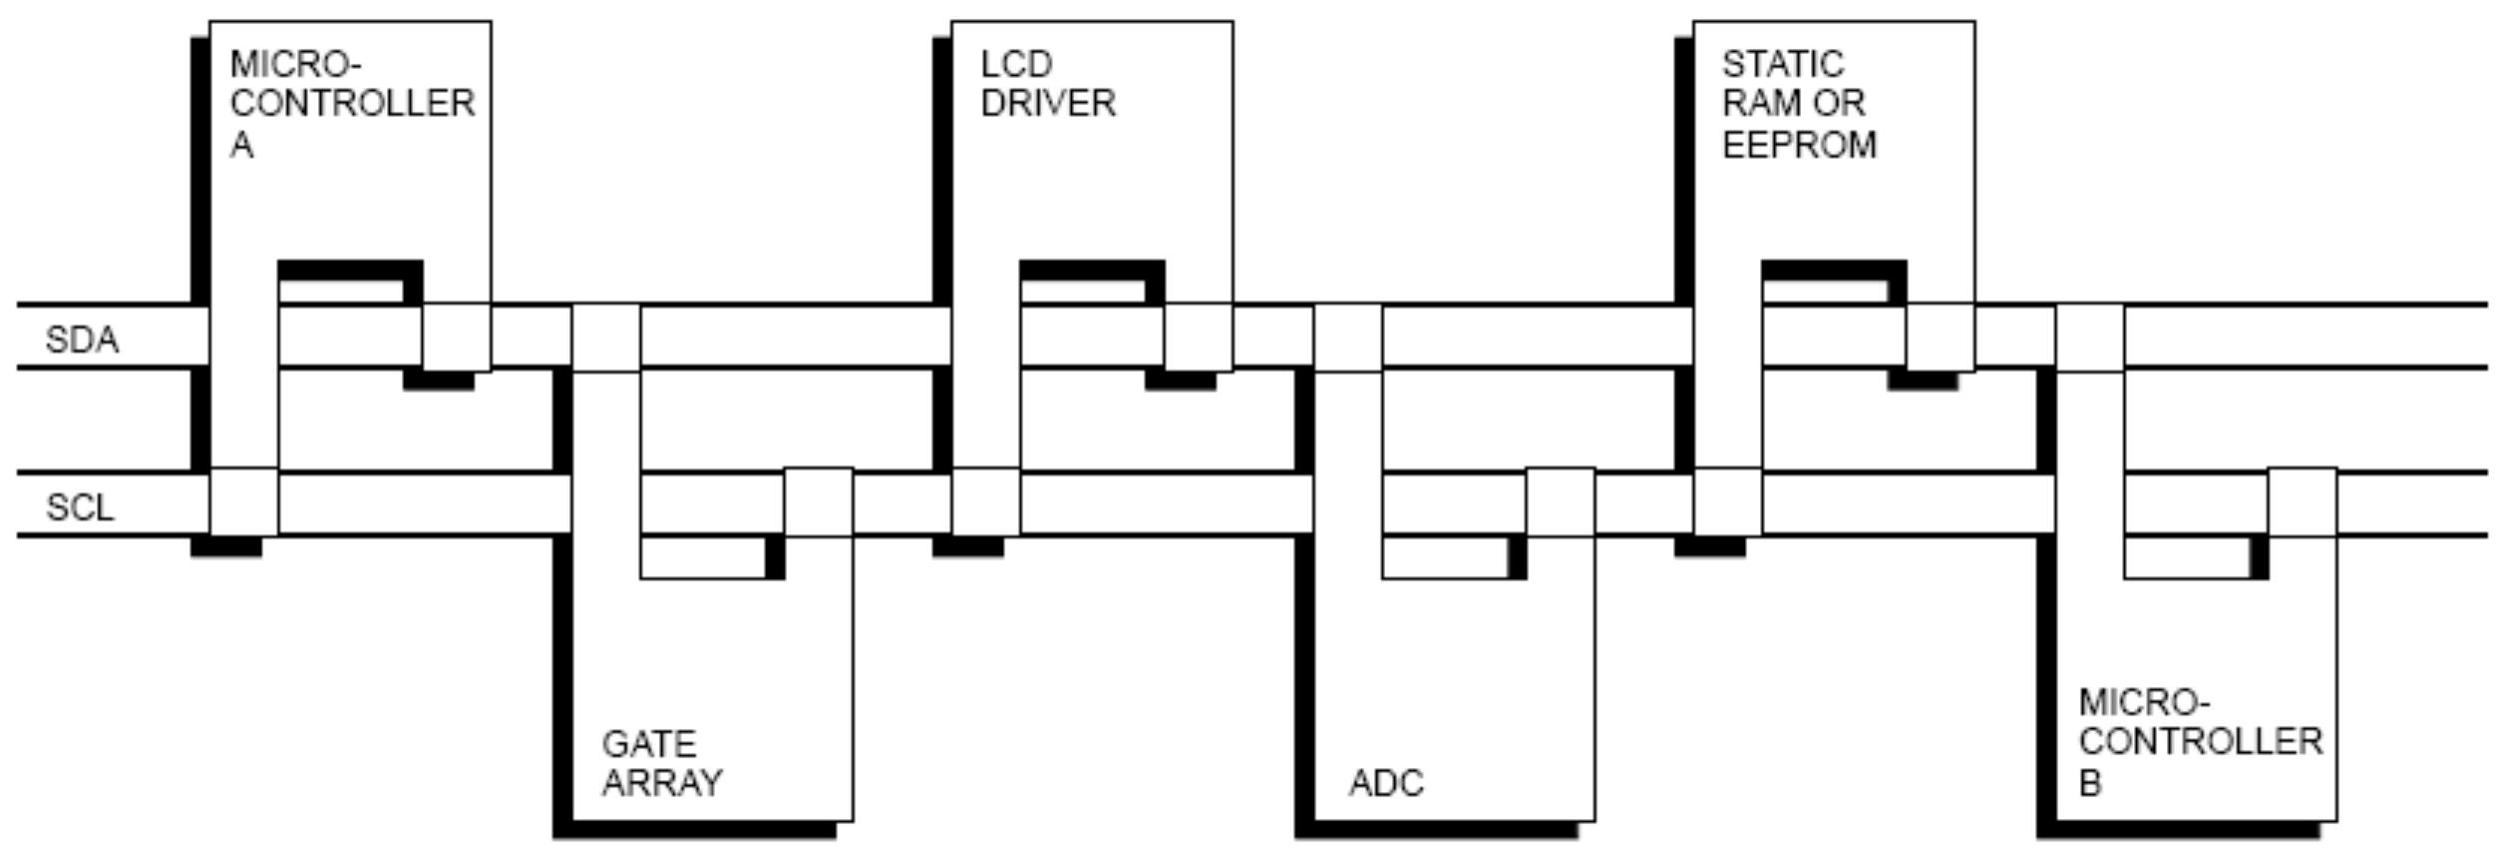
\includegraphics[max width=\textwidth]{2023_01_13_b07e3b4bcffdaab9792bg-246}
\end{center}

Example I2C-connected system with two microcontrollers

(Source: I2C Specification, Philips)


\os{newpage} item[{\rot\bf  Master-Slave Relationships }]~\\[-3ex]

\bi
  \ite Who is the master?
\ei
\bi
 \ite master-transmitters
 \ei

\bi
 \ite master-receivers
 \ei


\bi
  \ite Suppose microcontroller A wants to send information to microcontroller B

  \ite A (master) addresses B (slave)

\ei
\bi
 \ite A (master-transmitter), sends data to B (slave-receiver)
 \ei

\bi
 \ite A terminates the transfer.
 \ei


\bi
  \ite If microcontroller A wants to receive information from microcontroller B

  \ite A (master) addresses microcontroller B (slave)

  \ite A (master-receiver) receives data from B (slave-transmitter)

  \ite A terminates the transfer

  \ite In both cases, the master (microcontroller A) generates the timing and terminates the transfer

\ei


\os{newpage} item[{\rot\bf  Exercise: How fast can I2C run? }]~\\[-3ex]

\begin{center}
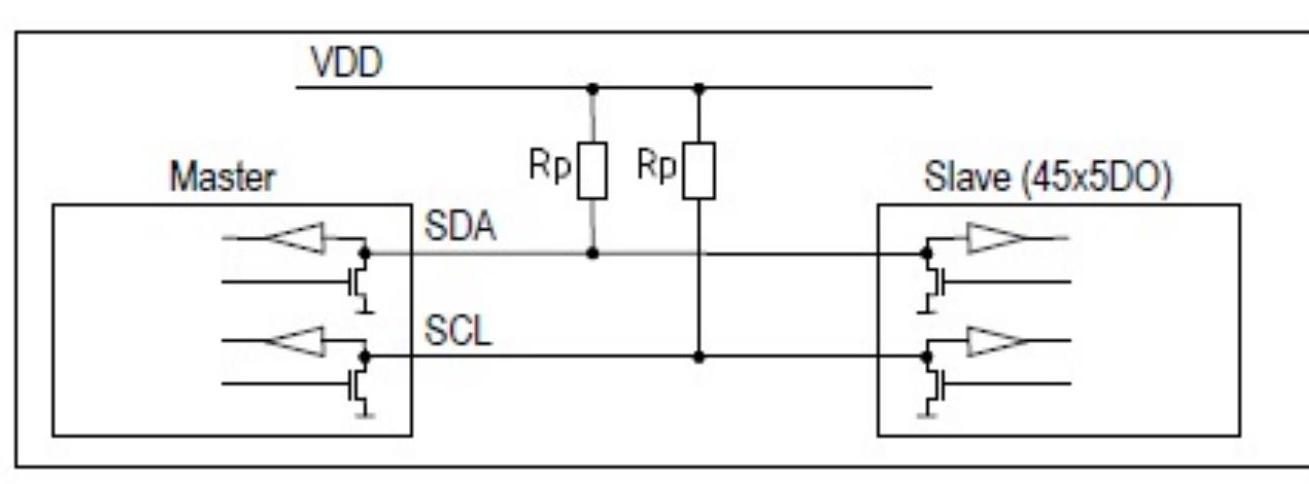
\includegraphics[max width=\textwidth]{2023_01_13_b07e3b4bcffdaab9792bg-248}
\end{center}

Capacitor charging in RC circuit

\begin{center}
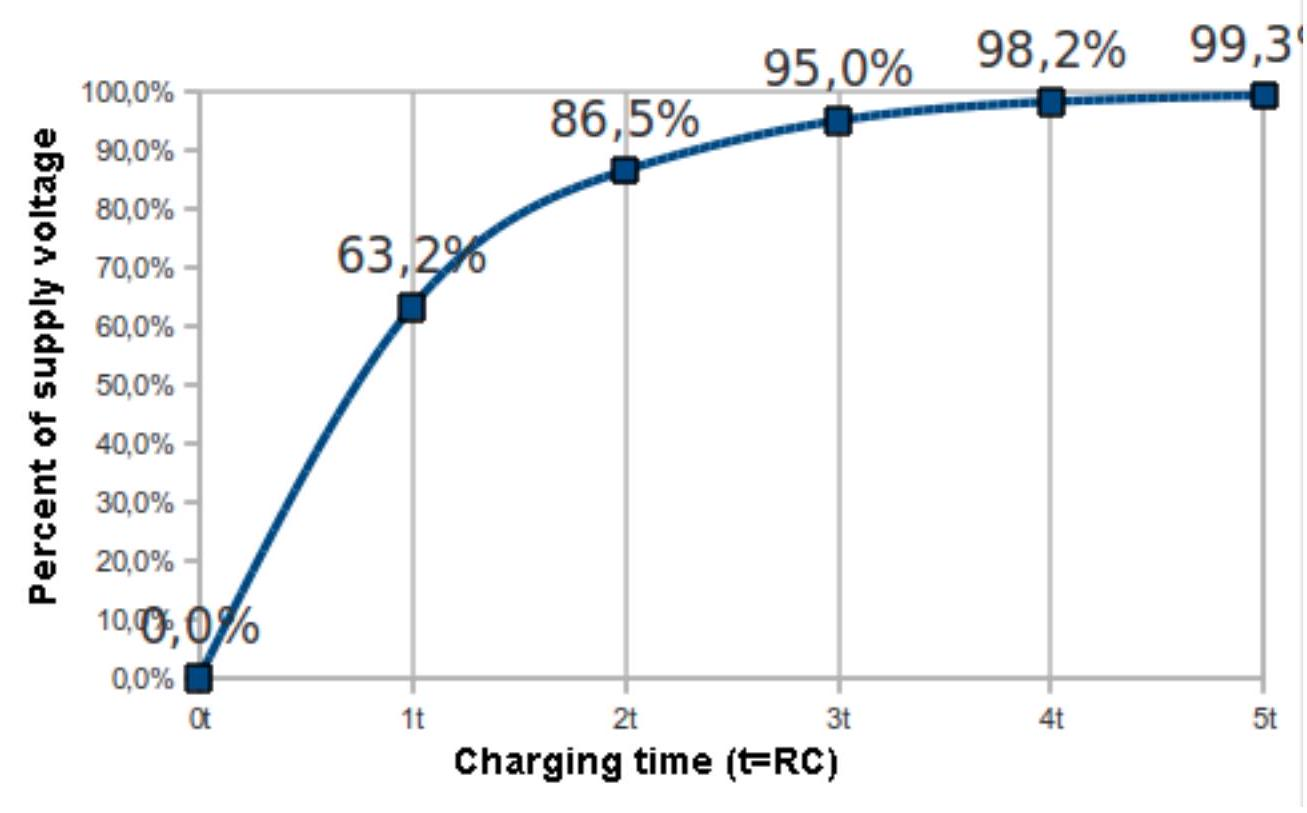
\includegraphics[max width=\textwidth]{2023_01_13_b07e3b4bcffdaab9792bg-248(1)}
\end{center}

\bi
  \ite How fast can you run it?

  \ite Assumptions

  \ite 0's are driven

  \ite 1's are "pulled up"

  \ite Some working figures

  \ite $\mathrm{R}_{\mathrm{p}}=10 \mathrm{k} \Omega$

  \ite $\mathrm{C}_{\text {cap }}=100 \mathrm{pF}$

  \ite $V_{D D}=5 V$

  \ite $ V_{in_high }=3.5 ~V $

  \ite Recall for RC circuit

\ei

$-\mathrm{V}_{\text {cap }}(\mathrm{t})=\mathrm{V}_{\mathrm{DD}}\left(1-\mathrm{e}^{-\mathrm{t} / \mathrm{\tau}}\right)$

\bi
  \ite Where $\tau=R C$
\ei


\os{newpage} item[{\rot\bf  Exercise: Bus bit rate vs Useful data rate }]~\\[-3ex]

\bi
  \ite An I2C "transactions" involves the following bits

  \ite $\langle\mathrm{S}\rangle\langle\mathrm{A} 6: \mathrm{A} 0\rangle\langle\mathrm{R} / \mathrm{W}\rangle\langle\mathrm{A}\rangle\langle\mathrm{D} 7: \mathrm{D} 0\rangle\langle\mathrm{A}\rangle\langle\mathrm{F}\rangle$

  \ite Which of these actually carries useful data?

  \ite $\langle\mathrm{S}\rangle\langle\mathrm{A} 6: \mathrm{A} 0\rangle\langle\mathrm{R} / \mathrm{W}\rangle\langle\mathrm{A}\rangle\langle\mathrm{D} 7: \mathrm{D} 0\rangle\langle\mathrm{A}\rangle\langle\mathrm{F}\rangle$

  \ite So, if a bus runs at $400 \mathrm{kHz}$

  \ite What is the clock period?

  \ite What is the data throughput (i.e. data-bits/second)?

  \ite What is the bus "efficiency"?

\ei

\end{description}



%%%%%%%%%%%%%%%%%%%%%%%%%%%%%%%%%%%%%%%%%%%%%%%%%%%%%%%%%%%%%%%%%%%%%%%%%%
\chapter{Operating Systems}
%%%%%%%%%%%%%%%%%%%%%%%%%%%%%%%%%%%%%%%%%%%%%%%%%%%%%%%%%%%%%%%%%%%%%%%%%%%
\section{Operating Systems for Embedded Systems}
%%%%%%%%%%%%%%%%%%%%%%%%%%%%%%%%%%%%%%%%%%%%%%%%%%%%%%%%%%%%%%%%%%%%%%%%%%%
\nsl{Advances in microcontroller technology continue to open up new application fields for embedded systems. In parallel with this trend,
the equipment controlled by embedded systems has become more sophisticated, often incorporating many functions in one product.
As a result, embedded systems have grown in scale and complexity. Moreover, as products increasingly adopt digital technology,
advanced processors have enabled more of the processing to be implemented in software, making embedded systems all the more important.
\newline
This means, in new application the developer is more and more interested to do the software development
with the support of an operating system. Especially in large scale systems the effect on reducing development cost with an operating system is important.
\newline
Even in the small-scale embedded system field, the growing scale and complexity of software and the need for fast
development turnaround time have made improving software productivity a pressing need. The use of C and other high-level languages
have become increasingly common for this reason.
\newline
Real time operating systems fulfil all the requirements from the developer. They guarantee a response of the system in specific time.
The development cycle becomes much shorter if the user could do the development on the target. Cross-development involves the downloading
of the executable program on the target, testing it, changing it and repeating the same procedure once more for the next error
is not an optimal development cycle. Real time operating systems offer a good support for the debugging.
\newline
There exist only a few drawbacks if you are looking for appropriate real time operating system. The first most important disadvantages
of the most real time operating systems are the costs. The second one is that real time operating systems need virtual memory system which is in
special not available in small microcontrollers.
\newline
The virtual memory system itself is really suitable for general purpose applications like a desktop PC.
But for embedded systems a virtual memory system makes the application more difficult. In such systems really often an access to the hardware
is necessary (control interfaces). These programming aspects could only be done in the so called ``kernel-mode'' with the result that such
programs more dangerous (collapse of the operating system) and more difficult to test.
\newline
In this chapter we will discuss some aspects of operating systems and than come to the uCLinux or other ``embedded Linux Systems'', operating systems
for microcontroller with and without a virtual memory system.
}
\bigskip
\bi
	\ite a lot of embedded systems runs without a operating system
	\bi
		\ite only  small algorithm (e.g. 'control the window' open/close system in a car).
		\ite hard restrictions in the size of memory especially by 8- and 16-bit microcontrollers.
		\ite costs of an operating system.
	\ei
	\bigskip
	\ite reasons for the use of an operating system
	\bi
		\ite generally the same reasons why we need one for a traditional computer.
		\ite but in the case of embedded systems not all services of an operating systems are needed for any device.
		\ite embedded systems have a large variety of requirements and environments.
		\bi
			\ite critical applications with high functionality (medical applications, aircraft systems ..).
			\ite critical applications with small functionality (ABS, cardiac pacemaker ..).
			\ite not very critical applications with varying functionality (mobile phone microwave ofen, washing machine ..).
		\ei

	\ei
\ei

\begin{description}
\item[{\rot\bf Special operating system (OS) for embedded systems}]~\\[-3ex]
\bigskip
\bi
	\ite a standard OS (like Windows or Linux) isn't suitable because :
	\bi
		\ite monolithic kernel has too many features which are not necessary in a specific application.
		\ite monolithic kernel is not modular, fault-tolerant, configurable, modifiable.
		\ite needs too much memory space (virtual memory).
		\ite not designed for mission-critical applications.	
	\ei
\ei
\bigskip
\item[{\rot\bf Key features of an OS for embedded systems }]~\\[-3ex]
\bigskip
\bi
	\ite configurability \pr no single OS will fit all needs, so configurability needed
	\bi
		\ite simplest form \pr remove unused functions (by linker ?)
		\ite conditional compilation (using \#if and \#ifdef commands)
		\ite dynamic data might be replaced by static data
		\ite removes unnecessary functions or modules by a kernel programming (Linux, eCos, VxWORKS).
	\ei
	\bigskip
	\ite handling of device drivers
	\bi
		\ite access to interfaces.
		\ite device drivers handled by tasks instead of integrated drivers.
		\ite improve predictability; everything goes through scheduler.
  		\ite in embedded systems mostly a lot of different interfaces are available, so not every device needs support by all versions of the OS.
	\ei
\ei

\begin{figure}[!hbtp]
     \begin{center}
	  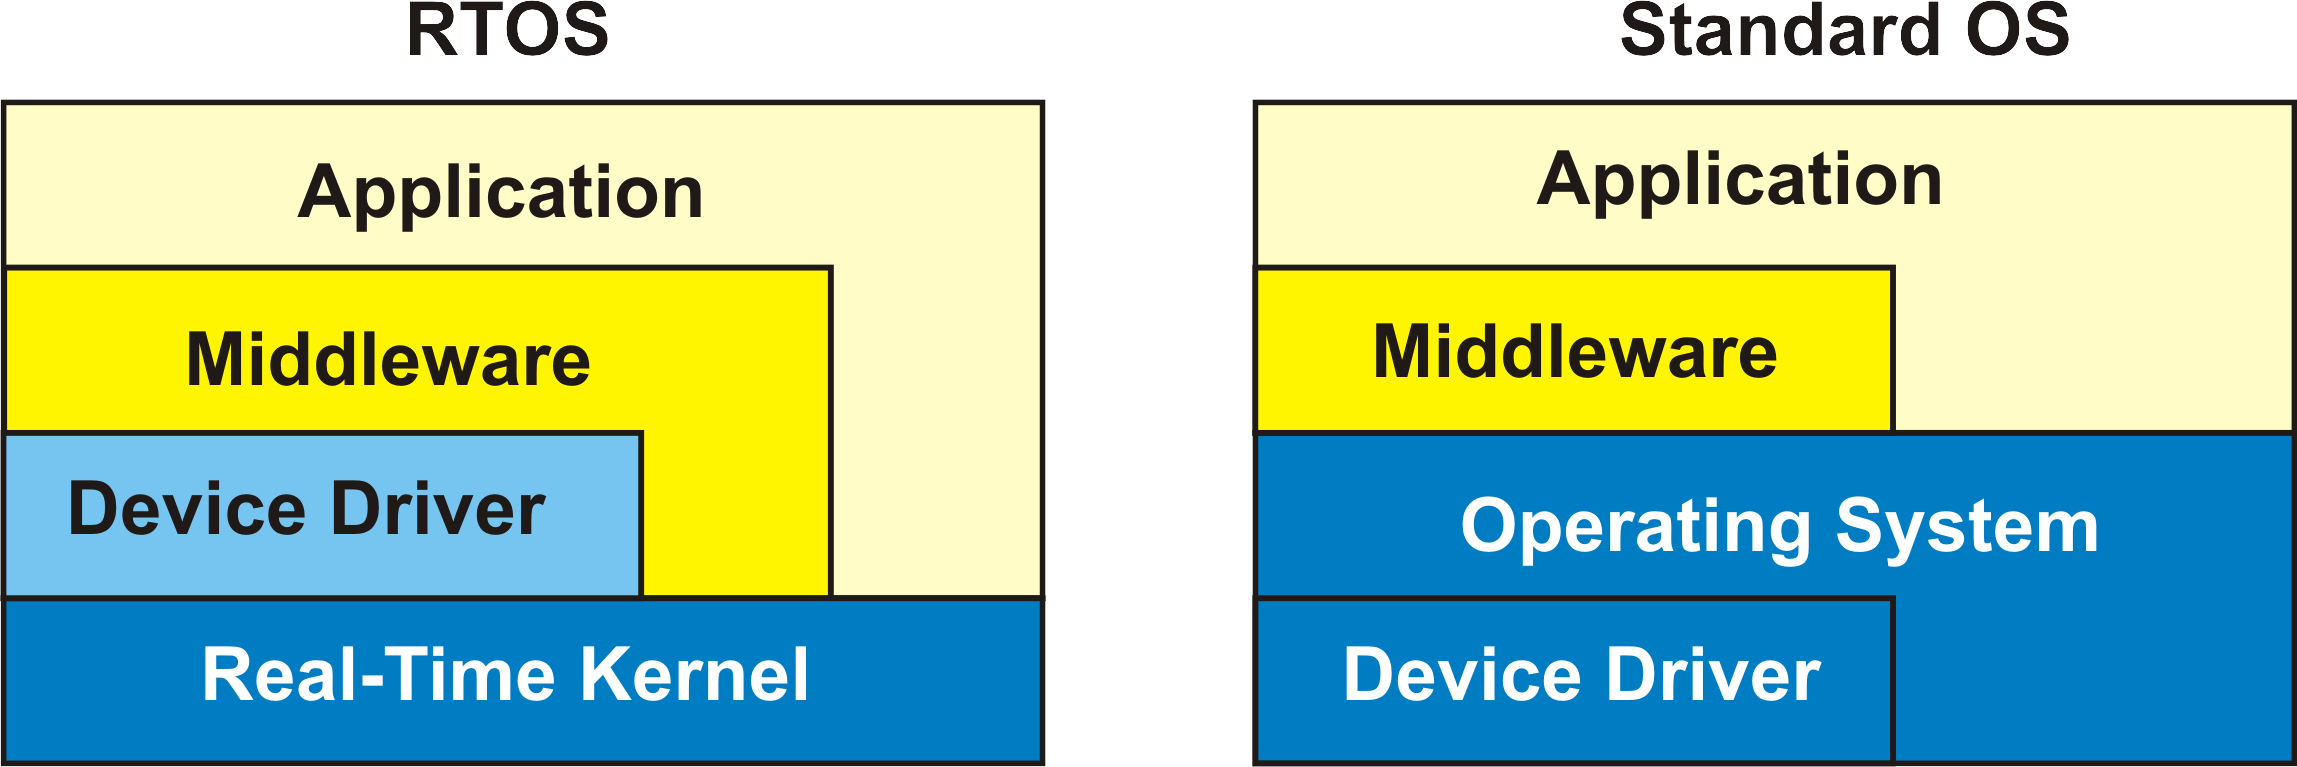
\epsfig{file=figures/Fig_6_1_RTOS_StandardOS,width=0.8\textwidth}\\
	  \caption{Integration of Devices Drivers in an OS}
     \end{center}
\end{figure}
\os{\newpage}

\bigskip
\bi
	\ite handling of interupts
	\bi
		\ite for standard OS: serious source of unreliability.
		\ite it should be possible to let interrupts directly start or stop tasks (by storing the tasks start address in the interrupt table).
	\ei
\ei

\item[{\rot\bf Available OS for embedded systems}]~\\[-3ex]
\bigskip
\bi
	\ite QNX
	\bi
		\ite real time operating system based on micro core technology.
		\ite suitable for small and large embedded systems.
		\ite tasks are separated in its one address space.
		\ite scheduling event driven (restrictions in time based scheduling) .
	\ei
	\bigskip
	\ite VxWORKS
	\bi
		\ite small VxWorks Kernel.
		\ite no virtual memory space (dangerous if a task is not cooperative).
		\ite scheduling time, priority and event driven.
		\ite implemented on a lot of microcontrollers.
	\ei
	\bigskip
	\ite OSEK/VDX
	\bi
		\ite scalable real time OS build for application in the automotive area.
		\ite event driven execution of tasks.
		\ite operates with fixed priorities.
		\ite tasks are grouped in basic tasks and extended tasks.
		\ite no virtual memory system.
	\ei
	\os{\newpage}
	\ite eCos
	\bi
		\ite open source system.
		\ite scalable system (the configuration allows the application writer to impose their requirements on the run-time component).
		\ite OS and application software are specific for an embedded system.
		\ite scheduling is time and event driven.
		\ite no virtual memory system.
	\ei
	\bigskip
	\ite embedded Linux
	\bi
		\ite open source system.
		\ite scalable and portable (especially for 32 bit microcontrollers).
		\ite run with a non virtual and a virtual memory system.
		\ite scheduling is time and priority driven.
		\ite with the RTAI (\underline{r}eal \underline{t}ime \underline{a}pplication \underline{i}nterface) also a event driven scheduling mechanismn possible.
		\ite for small and large embedded systems.
	\ei
\ei
\end{description}
\os{\newpage}

%%%%%%%%%%%%%%%%%%%%%%%%%%%%%%%%%%%%%%%%%%%%%%%%%%%%%%%%%%%%%%%%%%%%%%%%%%%
\section{Functions of RTOS}
%%%%%%%%%%%%%%%%%%%%%%%%%%%%%%%%%%%%%%%%%%%%%%%%%%%%%%%%%%%%%%%%%%%%%%%%%%%
\begin{description}


\item[{\rot\bf FreeRTOS}]~\\[-3ex]
\bi
\ite FreeRTOS is a real-time kernel/scheduler on top of which MCU applications can be built to meet their hard real-time requirements.
\bi
\ite Allows MCU applications be organized as a collection of independent threads of execution.
\ite Decides which thread should be executed by examining the priority assigned to each thread.
\bi
\ite Assume a single core MCU where only a single thread can be executing at one time.
\ei
\ei
\ei

\os{\newpage} \item[{\rot\bf The simplest case of task priority assignments}]~\\[-3ex]
\bi
\ite Assign higher priorities (lower priorities) to threads that implement hard real-time (soft real-time) requirements
\bi
\ite As a result hard real-time threads are always executed ahead of soft real-time threads.
\ei
\ite But priority assignment decision are not always that simple.
\ite In general task prioritization can help ensure an application meet its processing deadline.
\ei

\os{\newpage}



\item[{\rot\bf Why use a real-time kernel}]~\\[-3ex]
\bi
\ite For a simple system many well-established techniques can provide an  appropriate solution without the use of a kernel.
\ite For a more complex embedded application a kernel would be preferable.
\ite But where the crossover point occurs will always be subjective.
\ite Besides ensuring an application meets its processing deadline a kernel can bring other less obvious benefits.
\ei

\os{\newpage}



\item[{\rot\bf Benefits of using real-time kernel 1}]~\\[-3ex]
\bi
\ite Abstracting away timing information
\bi
\ite Kernel is responsible for execution timing and provides a time-related API to the application. This allows the application code to be simpler and the overall code size be smaller.
\ei
\ite Maintainability/Extensibility
\bi
\ite Abstracting away timing details results in fewer interdependencies between modules and allows sw to evolve in a predictable way.
\ite Application performance is less susceptible to changes in the underlying hardware.
\ei
\ite Modularity
\bi
\ite Tasks are independent modules each of which has a well-defined purpose.
\ei
\ite Team development
\bi
\ite Tasks have well-defined interfaces allowing easier development by teams
\ei
\ei

\os{\newpage}



\item[{\rot\bf Benefits of using real-time kernel 2}]~\\[-3ex]
\bi
\ite Easier testing
\bi
\ite Tasks are independent modules with clean interfaces they can be tested in isolation.
\ei
\ite Idle time utilization
\bi
\ite The idle task is created automatically when the kernel is started. It executes whenever there are no application tasks to run.
\ite Be used to measure spare processing capacity perform background checks or simply place the process into a low-power mode.
\ei
\ite Flexible interrupt handling
\bi
\ite Interrupt handlers can be kept very short by deferring most of the required processing to handler tasks.
\ei
\ei

\os{\newpage}



\item[{\rot\bf Standard FreeRTOS features}]~\\[-3ex]
\bi
\ite Pre-emptive or co-operative operation
\ite Very flexible task priority assignment
\ite Queues
\ite Binary/Counting / Recursive semaphores
\ite Mutexes
\ite Tick/Idle hook functions
\ite Stack overflow checking
\ite Trace hook macros
\ite Interrupt nesting
\ei

\os{\newpage}


\item[{\rot \bf FreeRTOS - RT and Embedded}]~\\[-3ex]
\bi
\ite "Embedded" and "real-time" can mean different things to different people, so let's define them as FreeRTOS uses them.
\ite An embedded system is a computer system that is designed to do only a few things, like the system in a TV remote control, in-car GPS, digital watch, or pacemaker. Embedded systems are typically smaller and slower than general purpose computer systems, and are also usually less expensive. A typical low-end embedded system may have an 8-bit CPU running at 25MHz, a few KB of RAM, and maybe 32KB of flash memory. A higher-end embedded system may have a 32-bit CPU running at 750MHz, a GB of RAM, and multiple GB of flash memory.
\ite Real-time systems are designed to do something within a certain amount of time; they guarantee that stuff happens when it's supposed to.
\ite A pacemaker is an excellent example of a real-time embedded system. A pacemaker must contract the heart muscle at the right time to keep you alive; it can't be too busy to respond in time. Pacemakers and other real-time embedded systems are carefully designed to run their tasks on time, every time.
\ei

\os{\newpage}



\item[{\rot\bf Architecture}]~\\[-3ex]
\bi
\ite FreeRTOS is a relatively small application. The minimum core of FreeRTOS is only three source (.c) files and a handful of header files, totalling just under 9000 lines of code, including comments and blank lines. A typical binary code image is less than 10KB.

\ite FreeRTOS's code breaks down into three main areas: tasks, communication, and hardware interfacing.

\ite Tasks: Almost half of FreeRTOS's core code deals with the central concern in many operating systems: tasks. A task is a user-defined C function with a given priority. tasks.c and task.h do all the heavy lifting for creating, scheduling, and maintaining tasks.

\ite Communication: Tasks are good, but tasks that can communicate with each other are even better! Which brings us to the second FreeRTOS job: communication. About 40\% of FreeRTOS's core code deals with communication. queue.c and queue.h handle FreeRTOS communication. Tasks and interrupts use queues to send data to each other and to signal the use of critical resources using semaphores and mutexes.

\ite The Hardware Whisperer: The approximately 9000 lines of code that make up the base of FreeRTOS are hardware-independent; the same code runs whether FreeRTOS is running on the humble 8051 or the newest, shiniest ARM core. About 6\% of FreeRTOS's core code acts a shim between the hardware-independent FreeRTOS core and the hardware-dependent code. We'll discuss the hardware-dependent code in the next section.
\ei

\os{\newpage}



\item[{\rot\bf Hardware Considerations}]~\\[-3ex]
\bi
\ite The hardware-independent FreeRTOS layer sits on top of a hardware-dependent layer. This hardware-dependent layer knows how to talk to whatever chip architecture you choose.
\ei
\begin{figure}[!hbtp]
     \begin{center}
	  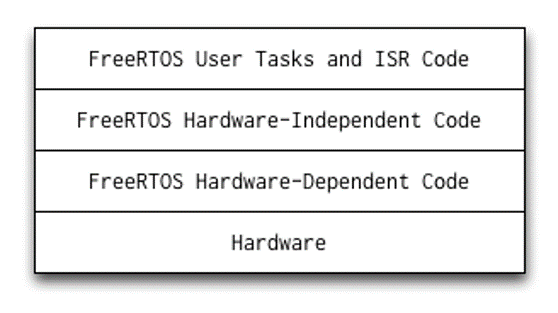
\epsfig{file=figures/Fig_6_1_00rtos.png,width=0.8\textwidth}\\
	  \caption{FreeRTOS Layers}
     \end{center}
\end{figure}

\os{\newpage}


\item[{\rot\bf Configurations}]~\\[-3ex]
\bi
\ite Configuration options are selected in FreeRTOSConfig.h by setting various \#defines. Clock speed, heap size, mutexes, and API subsets are all configurable in this file, along with many other options. Here are a few examples that set the maximum number of task priority levels, the CPU frequency, the system tick frequency, the minimal stack size and the total heap size:

\begin{lstlisting}[language=C]
#define configMax\_PRIORITIES     (( unsigned portBASE\_TYPE)5)
#define configCPU_CLOCK_HZ        (12000000UL)
#define configTICK_RATE_HZ        (( portTickType ) 1000)
#define configMINIMAL_STACK_SIZE  (( unsigned short ) 100)
#define configTOTAL\_HEAP\_SIZE   (( size_t ) ( 4 * 1024 ))
\end{lstlisting}
\ei

\os{\newpage}



\item[{\rot\bf Hardware Dependency}]~\\[-3ex]
\bi
\ite Hardware-dependent code lives in separate files for each compiler toolchain and CPU architecture.
\ite For example, if you're working with the IAR compiler on an ARM Cortex-M3 chip, the hardware-dependent code lives in the FreeRTOS/Source/portable/IAR/ARM\_CM3/ directory.
\ite portmacro.h declares all of the hardware-specific functions, while port.c and portasm.s contain all of the actual hardware-dependent code.
\ite The hardware-independent header file portable.h \#include's the correct portmacro.h file at compile time. FreeRTOS calls the hardware-specific functions using \#define'd functions declared in portmacro.h.
\ei

\os{\newpage}



\item[{\rot\bf Example}]~\\[-3ex]
\bi
\ite Let's look at an example of how FreeRTOS calls a hardware-dependent function. The hardware-independent file tasks.c frequently needs to enter a critical section of code to prevent preemption. Entering a critical section happens differently on different architectures, and the hardware-independent tasks.c does not want to have to understand the hardware-dependent details.
\ite So tasks.c calls the global macro portENTER\_CRITICAL(), glad to be ignorant of how it actually works.
\ite Assuming we're using the IAR compiler on an ARM Cortex-M3 chip, FreeRTOS is built with the file
\ite  FreeRTOS/Source/portable/IAR/ARM\_CM3/portmacro.h which defines portENTER\_CRITICAL() like this:
\ite \#define portENTER\_CRITICAL()   vPortEnterCritical()
\ei

\os{\newpage}



\item[{\rot\bf Example 2}]~\\[-3ex]
\bi
\ite vPortEnterCritical() is actually defined in
\bi
\ite FreeRTOS/Source/portable/IAR/ARM\_CM3/port.c.
\ite The port.c file is hardware-dependent, and contains code that understands the IAR compiler and the Cortex-M3 chip.
\ite vPortEnterCritical() enters the critical section using this hardware-specific knowledge and returns to the hardware-independent tasks.c.
\ei
\ite The portmacro.h file also defines an architecture's basic data types. Data types for basic integer variables, pointers, and the system timer tick data type are defined like this for the IAR compiler on ARM Cortex-M3 chips:
\begin{lstlisting}[language=C]
\ite #define portBASE\_TYPE  long              // Basic integer variable type
\ite #define portSTACK_TYPE unsigned long     // Pointers to memory locations
\ite typedef unsigned portLONG portTickType;  // The system timer tick type
\end{lstlisting}
\ei

\os{\newpage}



\item[{\rot\bf Example 3}]~\\[-3ex]
\bi
\ite This method of using data types and functions through thin layers of \#defines may seem a bit complicated, but it allows FreeRTOS to be recompiled for a completely different system architecture by changing only the hardware-dependent files. And if you want to run FreeRTOS on an architecture it doesn't currently support, you only have to implement the hardware-dependent functionality which is much smaller than the hardware-independent part of FreeRTOS.
\ite As we've seen, FreeRTOS implements hardware-dependent functionality with C preprocessor \#define macros. FreeRTOS also uses \#define for plenty of hardware-independent code. For non-embedded applications this frequent use of \#define is a cardinal sin, but in many smaller embedded systems the overhead for calling a function is not worth the advantages that "real" functions offer.
\ei

\os{\newpage}



\item[{\rot\bf Full task state machine}]~\\[-3ex]
\begin{center}
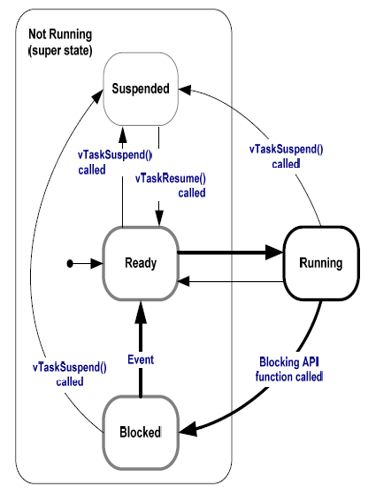
\includegraphics[height=12 cm]{figures/Fig_6_1_07rtos.png}
\end{center}

\os{\newpage}



{\rot \bf Tasks - Task Control Block in tasks.c}

\begin{lstlisting}[language=C]

typedef struct tskTaskControlBlock
{
   volatile portSTACK_TYPE *pxTopOfStack;      /* Points to the location of the last item placed on the tasks stack.  THIS MUST BE THE FIRST MEMBER OF THE STRUCT. */

   xListItem    xGenericListItem;                          /* List item used to place
                                                              the TCB in ready and
                                                              blocked queues. */
   xListItem    xEventListItem;                            /* List item used to place
                                                              the TCB in event lists.*/
   unsigned portBASE\_TYPE uxPriority;                      /* The priority of the task
                                                              where 0 is the lowest
                                                              priority. */
   portSTACK_TYPE *pxStack;                                /* Points to the start of
                                                              the stack. */
   signed char    pcTaskName[ configMAX_TASK\_NAME_LEN ];   /* Descriptive name given
                                                              to the task when created.
                                                              Facilitates debugging
                                                              only. */

   #if ( portSTACK_GROWTH > 0 )
     portSTACK_TYPE *pxEndOfStack;                         /* Used for stack overflow
                                                              checking on architectures
                                                              where the stack grows up
                                                              from low memory. */
   #endif

   #if ( configUSE_MUTEXES == 1 )
     unsigned portBASE\_TYPE uxBasePriority;                /* The priority last
                                                              assigned to the task -
                                                              used by the priority
                                                              inheritance mechanism. */
   #endif

 } tskTCB;

\end{lstlisting}


\os{\newpage}


\item[{\rot \bf Scheduling Tasks - Priorities and Ready List}]~\\[-3ex]
\bi
\ite Each task has a user-assigned priority between 0 (the lowest priority) and the compile-time value of configMAX\_PRIORITIES-1 (the highest priority). For instance, if configMAX\_PRIORITIES is set to 5, then FreeRTOS will use 5 priority levels: 0 (lowest priority), 1, 2, 3, and 4 (highest priority).

\ite FreeRTOS uses a "ready list" to keep track of all tasks that are currently ready to run. It implements the ready list as an array of task lists like this:
\ei

\begin{lstlisting}[language=C]
static xList pxReadyTasksLists[ configMax\_PRIORITIES ];  /* Prioritised ready tasks.  */
pxReadyTasksLists[0] is a list of all ready priority 0 tasks,
pxReadyTasksLists[1] is a list of all ready priority 1 tasks, and so on, all the way up to pxReadyTasksLists[configMax\_PRIORITIES-1].
\end{lstlisting}

\os{\newpage}



\item[{\rot\bf Scheduling Tasks - System Tick}]~\\[-3ex]

\bi
\ite The heartbeat of a FreeRTOS system is called the system tick. FreeRTOS configures the system to generate a periodic tick interrupt. The user can configure the tick interrupt frequency, which is typically in the millisecond range. Every time the tick interrupt fires, the vTaskSwitchContext() function is called. vTaskSwitchContext() selects the highest-priority ready task and puts it in the pxCurrentTCB variable like this:
\begin{lstlisting}[language=C]
 /* Find the highest-priority queue that contains ready tasks. */
 while( listLIST_IS_EMPTY( \&( pxReadyTasksLists[ uxTopReadyPriority ] ) ) )
 {
     configASSERT( uxTopReadyPriority );
     --uxTopReadyPriority;
 }

 /* listGET_OWNER_OF_NEXT_ENTRY walks through the list, so the tasks of the same
 priority get an equal share of the processor time. */
 listGET_OWNER_OF_NEXT_ENTRY( pxCurrentTCB, \&( pxReadyTasksLists[ uxTopReadyPriority ] ) );
\end{lstlisting}
\ei

\os{\newpage}



\item[{\rot\bf Scheduling Tasks - Ready List}]~\\[-3ex]
\bi
\ite Before the while loop starts, uxTopReadyPriority is guaranteed to be greater than or equal to the priority of the highest-priority ready task. The while() loop starts at priority level uxTopReadyPriority and walks down through the pxReadyTasksLists array to find the highest-priority level with ready tasks. listGET\_OWNER\_OF\_NEXT\_ENTRY() then grabs the next ready task from that priority level's ready list.

\ite Now pxCurrentTCB points to the highest-priority task, and when vTaskSwitchContext() returns the hardware-dependent code starts running that task.
\ite Those nine lines of code are the absolute heart of FreeRTOS. The other 8900+ lines of FreeRTOS are there to make sure those nine lines are all that's needed to keep the highest-priority task running.
\ei

\os{\newpage}




\nsl{

{\rot\bf Tasks - TCB}
\bi
\ite The TCB stores the address of the stack start address in pxStack and the current top of stack in pxTopOfStack. It also stores a pointer to the end of the stack in pxEndOfStack to check for stack overflow if the stack grows "up" to higher addresses. If the stack grows "down" to lower addresses then stack overflow is checked by comparing the current top of stack against the start of stack memory in pxStack.
\ite The TCB stores the initial priority of the task in uxPriority and uxBasePriority. A task is given a priority when it is created, and a task's priority can be changed. If FreeRTOS implements priority inheritance then it uses uxBasePriority to remember the original priority while the task is temporarily elevated to the "inherited" priority. (See the discussion about mutexes below for more on priority inheritance.)
\ite Each task has two list items for use in FreeRTOS's various scheduling lists. When a task is inserted into a list FreeRTOS doesn't insert a pointer directly to the TCB. Instead, it inserts a pointer to either the TCB's xGenericListItem or xEventListItem. These xListItem variables let the FreeRTOS lists be smarter than if they merely held a pointer to the TCB. We'll see an example of this when we discuss lists later.
\ite A task can be in one of four states: running, ready to run, suspended, or blocked. You might expect each task to have a variable that tells FreeRTOS what state it's in, but it doesn't. Instead, FreeRTOS tracks task state implicitly by putting tasks in the appropriate list: ready list, suspended list, etc. The presence of a task in a particular list indicates the task's state. As a task changes from one state to another, FreeRTOS simply moves it from one list to another.
\ei
}

\os{\newpage}



\item[{\rot\bf Tasks Setup}]~\\[-3ex]
\bi
\ite We've already touched on how a task is selected and scheduled with the pxReadyTasksLists array; now let's look at how a task is initially created. A task is created when the xTaskCreate() function is called. FreeRTOS uses a newly allocated TCB object to store the name, priority, and other details for a task, then allocates the amount of stack the user requests (assuming there's enough memory available) and remembers the start of the stack memory in TCB's pxStack member.
\ite The stack is initialized to look as if the new task is already running and was interrupted by a context switch. This way the scheduler can treat newly created tasks exactly the same way as it treats tasks that have been running for a while; the scheduler doesn't need any special case code for handling new tasks.
\ite The way that a task's stack is made to look like it was interrupted by a context switch depends on the architecture FreeRTOS is running on, but this ARM Cortex-M3 processor's implementation is a good example:
\ei

\os{\newpage}



\item[{\rot\bf Tasks - Stack}]~\\[-3ex]
\begin{lstlisting}[language=C]
 unsigned int *pxPortInitialiseStack( unsigned int *pxTopOfStack,
                                      pdTASK\_CODE pxCode,
                                      void *pvParameters )
 {
   /* Simulate the stack frame as it would be created by a context switch interrupt. */
   pxTopOfStack--; /* Offset added to account for the way the MCU uses the stack on
                      entry/exit of interrupts. */
   *pxTopOfStack = portINITIAL_XPSR;  /* xPSR */
   pxTopOfStack--;
   *pxTopOfStack = ( portSTACK_TYPE ) pxCode;  /* PC */
   pxTopOfStack--;
   *pxTopOfStack = 0;  /* LR */
   pxTopOfStack -= 5;  /* R12, R3, R2 and R1. */
   *pxTopOfStack = ( portSTACK_TYPE ) pvParameters;  /* R0 */
   pxTopOfStack -= 8;  /* R11, R10, R9, R8, R7, R6, R5 and R4. */

   return pxTopOfStack;
 }
\end{lstlisting}

\os{\newpage}



\item[{\rot\bf Tasks - Stack}]~\\[-3ex]
\bi
\ite The ARM Cortex-M3 processor pushes registers on the stack when a task is interrupted. pxPortInitialiseStack() modifies the stack to look like the registers were pushed even though the task hasn't actually started running yet. Known values are stored to the stack for the ARM registers xPSR, PC, LR, and R0. The remaining registers R1 -- R12 get stack space allocated for them by decrementing the top of stack pointer, but no specific data is stored in the stack for those registers. The ARM architecture says that those registers are undefined at reset, so a (non-buggy) program will not rely on a known value.
\ite After the stack is prepared, the task is almost ready to run. First though, FreeRTOS disables interrupts: We're about to start mucking with the ready lists and other scheduler structures and we don't want anyone else changing them underneath us.
\ite If this is the first task to ever be created, FreeRTOS initializes the scheduler's task lists. FreeRTOS's scheduler has an array of ready lists, pxReadyTasksLists, which has one ready list for each possible priority level. FreeRTOS also has a few other lists for tracking tasks that have been suspended, killed, and delayed. These are all initialized now as well.
\ite After any first-time initialization is done, the new task is added to the ready list at its specified priority level. Interrupts are re-enabled and new task creation is complete.
\ei

\os{\newpage}




\item[{\rot\bf Lists}]~\\[-3ex]
\bi
\ite The FreeRTOS list is a standard circular doubly linked list with a couple of interesting additions. Here's a list element:
\begin{lstlisting}[language=C]
 struct xLIST_ITEM
 {
   portTickType xItemValue;              /* The value being listed.  In most cases used to sort the list in descending order. */
   volatile struct xLIST_ITEM * pxNext;  /* Pointer to the next xListItem in the list.  */
   volatile struct xLIST_ITEM * pxPrevious;/* Pointer to the previous xListItem in the list. */
   void * pvOwner;                       /* Pointer to the object (normally a TCB) that contains the list item.  There is therefore a two-way link between the object containing the list item and the list item itself. */
   void * pvContainer;                   /* Pointer to the list in which this list item is placed (if any). */
 };
\end{lstlisting}
\ei

\os{\newpage}



\item[{\rot\bf Lists}]~\\[-3ex]
\bi
\ite Each list element holds a number, xItemValue, that is the usually the priority of the task being tracked or a timer value for event scheduling. Lists are kept in high-to-low priority order, meaning that the highest-priority xItemValue (the largest number) is at the front of the list and the lowest priority xItemValue (the smallest number) is at the end of the list.
\ite The pxNext and pxPrevious pointers are standard linked list pointers. pvOwner is a pointer to the owner of the list element. This is usually a pointer to a task's TCB object. pvOwner is used to make task switching fast in vTaskSwitchContext(): once the highest-priority task's list element is found in pxReadyTasksLists, that list element's pvOwner pointer leads us directly to the TCB needed to schedule the task.
\ite pvContainer points to the list that this item is in. It is used to quickly determine if a list item is in a particular list. Each list element can be put in a list, which is defined as:
\begin{lstlisting}[language=C]
 typedef struct xLIST
 {
   volatile unsigned portBASE\_TYPE uxNumberOfItems;
   volatile xListItem * pxIndex;           /* Used to walk through the list.  Points to
                                              the last item returned by a call to
                                              pvListGetOwnerOfNextEntry (). */
   volatile xMiniListItem xListEnd;        /* List item that contains the maximum
                                              possible item value, meaning it is always
                                              at the end of the list and is therefore
                                              used as a marker. */
 } xList;
\end{lstlisting}
\ei

\os{\newpage}



\item[{\rot\bf Lists}]~\\[-3ex]
\bi
\ite The size of a list at any time is stored in uxNumberOfItems, for fast list-size operations. All new lists are initialized to contain a single element: the xListEnd element. xListEnd.xItemValue is a sentinel value which is equal to the largest value for the xItemValue variable: 0xffff when portTickType is a 16-bit value and 0xffffffff when portTickType is a 32-bit value. Other list elements may also have the same value; the insertion algorithm ensures that xListEnd is always the last item in the list.
\ite Since lists are sorted high-to-low, the xListEnd element is used as a marker for the start of the list. And since the list is circular, this xListEnd element is also a marker for the end of the list.
\ite Most "traditional" list accesses you've used probably do all of their work within a single for() loop or function call like this:

\ei

\os{\newpage}

\item[{\rot\bf Lists}]~\\[-3ex]
\bi
\begin{lstlisting}[language=C]
for (listPtr = listStart; listPtr != NULL; listPtr = listPtr->next) {
   // Do something with listPtr here...
}
\end{lstlisting}
\ite FreeRTOS frequently needs to access a list across multiple for() and while() loops as well as function calls, and so it uses list functions that manipulate the pxIndex pointer to walk the list. The list function listGET\_OWNER\_OF\_NEXT\_ENTRY() does pxIndex = pxIndex->pxNext; and returns pxIndex. (Of course it does the proper end-of-list-wraparound detection too.) This way the list itself is responsible for keeping track of "where you are" while walking it using pxIndex, allowing the rest of FreeRTOS to not worry about it.
\ei

\os{\newpage}




\item[{\rot\bf Lists}]~\\[-3ex]
\bi
\ite The pxReadyTasksLists list manipulation done in vTaskSwitchContext() is a good example of how pxIndex is used. Let's assume we have only one priority level, priority 0, and there are three tasks at that priority level. This is similar to the basic ready list picture we looked at earlier, but this time we'll include all of the data structures and fields.
\ite As you can see in Figure 3.3, pxCurrentTCB indicates that we're currently running Task B. The next time vTaskSwitchContext() runs, it calls $listGET_OWNER_OF_NEXT_ENTRY()$ to get the next task to run. This function uses pxIndex->pxNext to figure out the next task is Task C, and now pxIndex points to Task C's list element and pxCurrentTCB points to Task C's TCB, as shown in Figure 3.4.
\ite Note that each struct xListItem object is actually the xGenericListItem object from the associated TCB.
\ei

\os{\newpage}



\item[{\rot\bf Queues}]~\\[-3ex]
\bi
\ite FreeRTOS allows tasks to communicate and synchronize with each other using queues.
\ite Interrupt service routines (ISRs) also use queues for communication and synchronization.
\ite The basic queue data structure is:
\begin{lstlisting}[language=C]
 typedef struct QueueDefinition
 {
   signed char *pcHead;                      /* Points to the beginning of the queue storage area. */
   signed char *pcTail;                      /* Points to the byte at the end of the
                                                queue storage area. One more byte is
                                                allocated than necessary to store the
                                              queue items; this is used as a marker. */
   signed char *pcWriteTo;                   /* Points to the free next place in the
                                                storage area. */
   signed char *pcReadFrom;                  /* Points to the last place that a queued
                                                item was read from. */

   xList xTasksWaitingToSend;                /* List of tasks that are blocked waiting
                                                to post onto this queue.  Stored in
                                                priority order. */
   xList xTasksWaitingToReceive;             /* List of tasks that are blocked waiting
                                                to read from this queue. Stored in
                                                priority order. */

   volatile unsigned portBASE\_TYPE uxMessagesWaiting;  /* The number of items currently
                                                          in the queue. */
   unsigned portBASE\_TYPE uxLength;                    /* The length of the queue
                                                          defined as the number of
                                                          items it will hold, not the
                                                          number of bytes. */
   unsigned portBASE\_TYPE uxItemSize;                  /* The size of each items that
                                                          the queue will hold. */

 } xQUEUE;
\end{lstlisting}
\ei

\os{\newpage}



\item[{\rot\bf Queues}]~\\[-3ex]
\bi
\ite This is a fairly standard queue with head and tail pointers, as well as pointers to keep track of where we've just read from and written to.
\ite When creating a queue, the user specifies the length of the queue and the size of each item to be tracked by the queue. pcHead and pcTail are used to keep track of the queue's internal storage. Adding an item into a queue does a deep copy of the item into the queue's internal storage.
\ite FreeRTOS makes a deep copy instead of storing a pointer to the item because the lifetime of the item inserted may be much shorter than the lifetime of the queue. For instance, consider a queue of simple integers inserted and removed using local variables across several function calls. If the queue stored pointers to the integers' local variables, the pointers would be invalid as soon as the integers' local variables went out of scope and the local variables' memory was used for some new value.
\ite The user chooses what to queue. The user can queue copies of items if the items are small, or the user can queue pointers to the items if the items are large. Note that in both cases FreeRTOS does a deep copy: if the user chooses to queue copies of items then the queue stores a deep copy of each item; if the user chooses to queue pointers then the queue stores a deep copy of the pointer. Of course, if the user stores pointers in the queue then the user is responsible for managing the memory associated with the pointers. The queue doesn't care what data you're storing in it, it just needs to know the data's size.
\ei

\os{\newpage}



\item[{\rot\bf Queues}]~\\[-3ex]
\bi
\ite FreeRTOS supports blocking and non-blocking queue insertions and removals. Non-blocking operations return immediately with a "Did the queue insertion work?" or "Did the queue removal work?" status. Blocking operations are specified with a timeout. A task can block indefinitely or for a limited amount of time.
\ite A blocked task - call it Task A - will remain blocked as long as its insert/remove operation cannot complete and its timeout (if any) has not expired. If an interrupt or another task modifies the queue so that Task A's operation could complete, Task A will be unblocked. If Task A's queue operation is still possible by the time it actually runs then Task A will complete its queue operation and return "success". However, by the time Task A actually runs, it is possible that a higher-priority task or interrupt has performed yet another operation on the queue that prevents Task A from performing its operation. In this case Task A will check its timeout and either resume blocking if the timeout hasn't expired, or return with a queue operation "failed" status.
\ei

\os{\newpage}
\item[{\rot\bf Queues}]~\\[-3ex]
\bi
\ite It's important to note that the rest of the system keeps going while a task is blocking on a queue; other tasks and interrupts continue to run. This way the blocked task doesn't waste CPU cycles that could be used productively by other tasks and interrupts.
\ite FreeRTOS uses the xTasksWaitingToSend list to keep track of tasks that are blocking on inserting into a queue. Each time an element is removed from a queue the xTasksWaitingToSend list is checked. If a task is waiting in that list the task is unblocked.
\ite Similarly, xTasksWaitingToReceive keeps track of tasks that are blocking on removing from a queue. Each time a new element is inserted into a queue the xTasksWaitingToReceive list is checked. If a task is waiting in that list the task is unblocked.
\ei

\os{\newpage}



\item[{\rot\bf Semaphores and Mutexes}]~\\[-3ex]
\bi
\ite FreeRTOS uses its queues for communication between and within tasks.
\ite FreeRTOS also uses its queues to implement semaphores and mutexes.
\ite What's The Difference?
\ite Semaphores and mutexes may sound like the same thing, but they're not. FreeRTOS implements them similarly, but they're intended to be used in different ways. How should they be used differently?

\ite The correct use of a semaphore is for signaling from one task to another. A mutex is meant to be taken and released, always in that order, by each task that uses the shared resource it protects. By contrast, tasks that use semaphores either signal ["send" in FreeRTOS term or wait ["receive" in FreeRTOS term - not both.
\ite A mutex is used to protect a shared resource. A task acquires a mutex, uses the shared resource, then releases the mutex. No task can acquire a mutex while the mutex is being held by another task. This guarantees that only one task is allowed to use a shared resource at a time.
\ite Semaphores are used by one task to signal another task.
\ite For example, Task 1 may contain code to post (i.e., signal or increment) a particular semaphore when the "power" button is pressed and Task 2, which wakes the display, pends on that same semaphore. In this scenario, one task is the producer of the event signal; the other the consumer.
\ei

\os{\newpage}



\item[{\rot\bf Semaphores and Mutexes}]~\\[-3ex]
\bi
\ite FreeRTOS implements an N-element semaphore as a queue that can hold N items. It doesn't store any actual data for the queue items; the semaphore just cares how many queue entries are currently occupied, which is tracked in the queue's uxMessagesWaiting field. It's doing "pure synchronization", as the FreeRTOS header file semphr.h calls it. Therefore the queue has a item size of zero bytes (uxItemSize == 0). Each semaphore access increments or decrements the uxMessagesWaiting field; no item or data copying is needed.
\ite Like a semaphore, a mutex is also implemented as a queue, but several of the xQUEUE struct fields are overloaded using \#defines:
\begin{lstlisting}[language=C]
\ite /* Effectively make a union out of the xQUEUE structure. */
\ite #define uxQueueType           pcHead
\ite #define pxMutexHolder         pcTail
\end{lstlisting}

\ite Since a mutex doesn't store any data in the queue, it doesn't need any internal storage, and so the pcHead and pcTail fields aren't needed. FreeRTOS sets the uxQueueType field (really the pcHead field) to 0 to note that this queue is being used for a mutex. FreeRTOS uses the overloaded pcTail fields to implement priority inheritance for mutexes.
\ei

\os{\newpage}



\item[{\rot\bf Priority Inheritance}]~\\[-3ex]
\bi
\ite In case you're not familiar with priority inheritance, I'll quote Michael Barr again to define it, this time from his article, "Introduction to Priority Inversion":
\ite [Priority inheritance] mandates that a lower-priority task inherit the priority of any higher-priority task pending on a resource they share. This priority change should take place as soon as the high-priority task begins to pend; it should end when the resource is released.
\ite FreeRTOS implements priority inheritance using the pxMutexHolder field (which is really just the overloaded-by-\#define pcTail field). FreeRTOS records the task that holds a mutex in the pxMutexHolder field. When a higher-priority task is found to be waiting on a mutex currently taken by a lower-priority task, FreeRTOS "upgrades" the lower-priority task to the priority of the higher-priority task until the mutex is available again.
\ei

\os{\newpage}



\item[{\rot\bf Task management}]~\\[-3ex]

\bi
\ite Introduction and scope
\ite Main topics to be covered
\bi
\ite How FreeRTOS allocates processing time to each task within an application
\ite How FreeRTOS chooses which task should execute at any given time
\ite How the relative priority of each task affects system behavior
\ite The states that a task can exist in.
\ei
\ei

\os{\newpage}



\item[{\rot\bf More specific topics }]~\\[-3ex]
\bi
\ite How to implement tasks
\ite How to create one or more instances of a task
\ite How to use the task parameter
\ite How to change the priority of a task that has already been created.
\ite How to delete a task.
\ite How to implement periodic processing.
\ite When the idle task will execute and how it can be used.
\ei

\os{\newpage}



\item[{\rot\bf Task functions}]~\\[-3ex]
\bi
\ite Tasks are implemented as C functions.
\bi
\ite Special: Its prototype must return void and take a void pointer parameter as the following
\ite void ATaskFunction (void *pvParameters);
\ei
\ite Each task is a small program in its own right.
\bi
\ite Has an entry point
\ite Normally runs forever within an infinite loop
\ite Does not exit
\ei
\ei

\os{\newpage}



\item[{\rot\bf Special features of task function}]~\\[-3ex]
\bi
\ite FreeRTOS task
\bi
\ite Must not contain a "return" statement
\ite Must not be allowed to execute past the end of the function
\ite If a task is no longer required it should be explicitly deleted.
\ite Be used to create any number of tasks
\bi
\ite Each created task is a separate execution instance with its own stack and its own copy of any automatic variables defined within the task itself.
\ei
\ei
\ei

\os{\newpage}




\item[{\rot\bf Top level task states}]~\\[-3ex]
\bi
\ite A task can exist in one of two states: Running and Not Running
\ite Scheduler is the only entity that can switch a task in and out a running state.
\ei
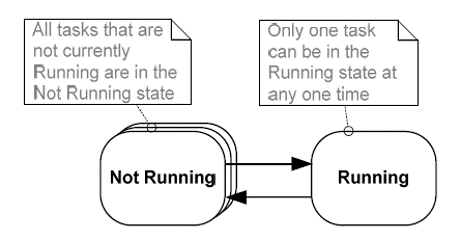
\includegraphics{figures/Fig_6_1_02rtos.png}
\bi
\ite Running state: the processor is
\ite executing its code.
\ite Not Running state: the task is dormant  its status having been saved ready for resuming execution the next time
\ei

\os{\newpage}



\item[{\rot\bf Creating Tasks}]~\\[-3ex]
\bi
\ite xTaskCreate() API function
\bi
\ite the most fundamental component in a multitasking system
\bi
\ite Probably the most complex of all API functions
\ite
\ei
\begin{lstlisting}[language=C]
 portBASE\_TYPE  xTaskCreate(
 pdTASK\_CODE 	pvTaskCode
 const signed char 	* const pcName
 unsigned short 		usStackDepth
 void 			*pvParameters
 unsigned portBASE\_TYPE uxPriority
 xTaskHandle 		*pxCreatedTask
 );
\end{lstlisting}
\ei
\ei

\os{\newpage}



\item[{\rot\bf All parameters}]~\\[-3ex]
\bi
\ite pvTaskCode
\bi
\ite a pointer to the function (just the function name) that implements the task.
\ei
\ite pcName
\bi
\ite A descriptive name for the task. It is not used by FreeRTOS but a debugging aid.
\ite configMAX\_TASK\_NAME\_LEN: the application defined constant that defines the maximum length a task name can task including the NULL terminator.
\ei
\ei

\os{\newpage}



\item[{\rot\bf All parameters}]~\\[-3ex]
\bi
\ite usStackDepth
\bi
\ite Each task has its own unique stack that is allocated by the kernel to the task when the task is created.
\ite The value specifies the number of words the task stack can hold.
\bi
\ite E.g. Cortex-M3 stack is 32 bits wide if usStackDepth is passed in as 100 400 bytes of stack space will be allocated (100*4 bytes)
\ei
\ite Size of the stack used by the idle task is defined by configMINIMAL\_STACK\_SIZE.
\bi
\ite Adjustable w.r.t. applications
\ei
\ei
\ei

\os{\newpage}



\item[{\rot\bf All parameters}]~\\[-3ex]
\bi
\ite pvParameters
\bi
\ite The value assigned to pvParameters will be the values passed into the task.
\ei
\ite uxPriority
\bi
\ite defines the priority at which the task will execute.
\ite Priorities can be assigned from 0 which is the lowest priority to (configMAX\_PRIOIRTIES-1) which is the highest priority.
\ite Passing a value above (configMAX\_PRIOIRTIES -1) will result in the priority being capped the maximum legitimate value.
\ei
\ei

\os{\newpage}



\item[{\rot\bf All parameters}]~\\[-3ex]
\bi
\ite pxCreatedTask
\bi
\ite pass out a handle to the created task then be used to refer the created task in API calls.
\bi
\ite E.g. change the task priority or delete the task
\ei
\ite Be set to NULL if no use for the task handle
\ite
\ei
\ite Two possible return values
\bi
\ite pdTRUE : task has been created successfully.
\ite errCOULD\_NOT\_ALLOCATE\_REQUIRED\_MEMORY
\bi
\ite Task has not been created as there is insufficient heap memory available for FreeRTOS to allocate enough RAM to hold the task data structures and stack.
\ei
\ei
\ei

\os{\newpage}



\item[{\rot\bf Example: Creating tasks}]~\\[-3ex]
\bi
\ite To demonstrate the steps of creating two tasks then starting the tasks executing.
\bi
\ite Tasks simply print out a string periodically using a crude null loop to create the periodic delay.
\ite Both tasks are created at the same priority and are identical except for the string they print out.
\ei
\ei

\os{\newpage}



\item[{\rot\bf Execution pattern of two Example 1 tasks}]~\\[-3ex]
\bi
\ite Both tasks are rapidly entering and exiting the Running state.
\ite Only one task can exist in the Running state at any one time.
\ei
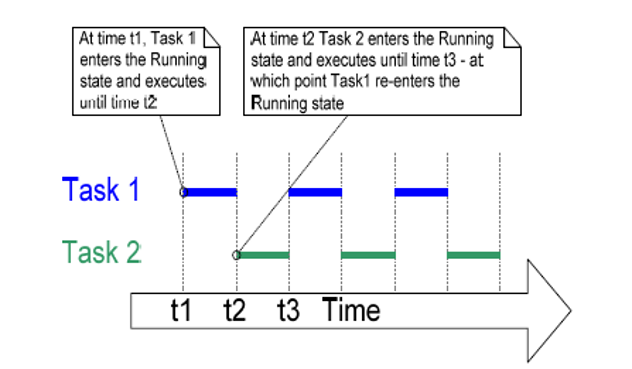
\includegraphics{figures/Fig_6_1_03rtos.png}

\os{\newpage}



\item[{\rot\bf Example 2 Using the task parameter}]~\\[-3ex]
\bi
\ite The two tasks in Example 1 are almost identical the only difference between them being the text string they print out.
\bi
\ite Remove such duplication by creating two instances of a single task implementation vTaskFunction.
\bi
\ite Each created instance will execute independently under the control of the FreeRTOS scheduler.
\ei
\ite The task parameter can then be used to pass into each task the string that it should print out.
\ei
\ei

\os{\newpage}



\item[{\rot\bf Example 2 Using the task parameter}]~\\[-3ex]
\bi
\ite First define a char string pcTextForTask1
\ite static const char *pcTextForTask1 = Task 1 is running.;
\ite Then in main(void) function change
\ite xTaskCreate( vTask1 Task 1 240 NULL 1 NULL );
\ite to
\ite xTaskCreate( vTaskFunction Task 1 240 (void*)pcTextForTask1 1 NULL );
\ite Create a task function vTaskFunction(void * pvParameters)
\ite char *pcTaskName;
\ite pcTaskName = (char *) pvParameters;
\ite
\ite
\ei

\os{\newpage}



\item[{\rot\bf Task priorities}]~\\[-3ex]
\bi
\ite uxPriority parameter of xTaskCreate() assigns an initial priority to the task being created.
\bi
\ite It can be changed after the scheduler has been started by using vTaskPrioritySet() API function
\ite
\ei
\ite configMax\_PRIORITIES in FreeRTOSConfig.h
\bi
\ite Maximum number of priorities
\ite Higher this value more RAM consumed
\ite Range: [0(low) configMAX\_PRIORITIES-1(high)]
\ite Any number of tasks can share the same priority
\ei
\ei

\os{\newpage}



\item[{\rot\bf Task priorities}]~\\[-3ex]
\bi
\ite To select the next task to run the scheduler itself must execute at the end of each time slice.
\bi
\ite Use a periodic interrupt called the tick (interrupt).
\ite Effectively set the length of time slice by the tick interrupt frequency -- configTICK\_RATE\_HZ in FreeRTOSConfig.h
\ei
\ite configTICK\_RATE\_HZ
\bi
\ite If it is 100(Hz) the time slice will be 10 ms.
\ite API always calls specify time in tick interrupts (ticks)
\ei
\ite portTICK\_RATE\_MS
\bi
\ite Convert time delays from milliseconds into the number of tick interrupts.
\ei
\ei

\os{\newpage}



\item[{\rot\bf Task priorities}]~\\[-3ex]
\bi
\ite When kernel itself is running the arrows in the above figure show the sequence of execution from task interrupt then from interrupt back to a next task.
\ei
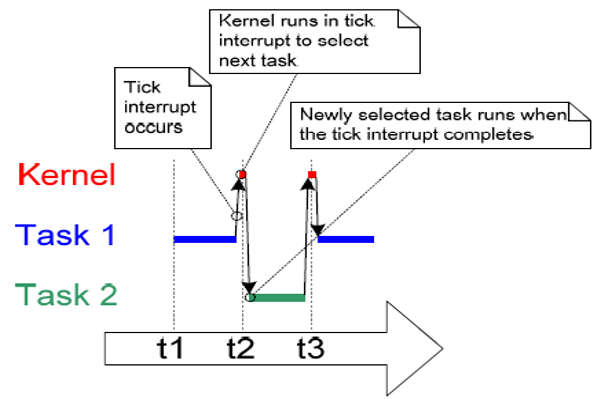
\includegraphics{figures/Fig_6_1_04rtos.png}

\os{\newpage}



\item[{\rot\bf Example 3. Experimenting with priorities}]~\\[-3ex]
\bi
\ite Scheduler always ensures that the highest priority task is able to run is the task selected to enter the Running state.
\bi
\ite In Example 1 and 2 two tasks have been created at the same priority so both entered and exited the Running state in turn.
\ite In this example the second task is set at priority 2.
\ei
\ei

\os{\newpage}



\item[{\rot\bf Example 3. Experimenting with priorities}]~\\[-3ex]
\bi
\ite In main() function change
\bi
\ite xTaskCreate( vTaskFunction Task 2 240 (void*)pcTextForTask2 1 NULL );
\ite To
\ite xTaskCreate( vTaskFunction Task 2 240 (void*)pcTextForTask2 2 NULL );
\ite
\ei
\ei

\os{\newpage}



\item[{\rot\bf Example 3. Experimenting with priorities}]~\\[-3ex]
\bi
\ite The scheduler always selects the highest priority task that is able to run.
\bi
\ite Task 2 has a higher priority than Task 1; so Task 2 is the only task to ever enter the Running state.
\ite Task 1 is to be "starved" of processing time of Task 2.
\ei
\ei
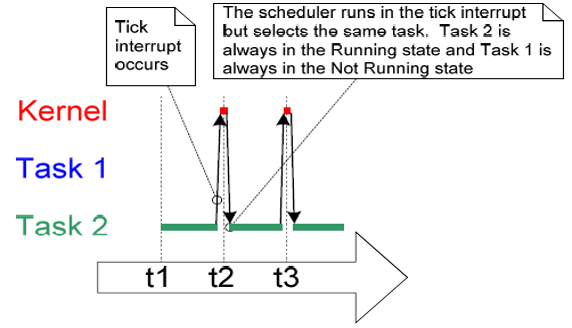
\includegraphics{figures/Fig_6_1_05rtos.png}

\os{\newpage}



\item[{\rot\bf"Continuous processing" task}]~\\[-3ex]
\bi
\ite So far the created tasks always have work to perform and have never had to wait for anything
\bi
\ite Always able to enter the Running state.
\ei
\ite This type of task has limited usefulness as they can only be created at the very lowest priority.
\bi
\ite If they run at any other priority they will tasks of lower priority  ever running at all.
\ei
\ite Solution: Event-driven tasks
\ei

\os{\newpage}



\item[{\rot\bf Expanding the "Not Running" state}]~\\[-3ex]
\bi
\ite An event-driven task
\bi
\ite has work to perform only after the occurrence of the event that triggers it
\ite Is not able enter the Running state before that event has occurred.
\ei
\ite The scheduler selects the highest priority task that is able to run.
\bi
\ite High priority tasks not being able to run means that the scheduler cannot select them and
\ite Must select a lower priority task that is able to run.
\ei
\ite Using event-driven tasks means that
\bi
\ite tasks can be created at different priorities without the highest priority tasks starving all the lower priority tasks.
\ei
\ei

\os{\newpage}



\item[{\rot\bf Full task state machine}]~\\[-3ex]

\begin{centering}
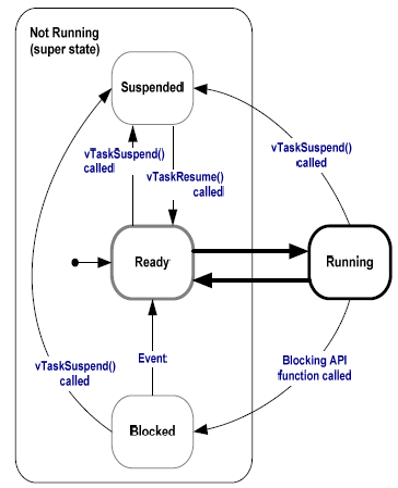
\includegraphics[height=12cm]{figures/Fig_6_1_08rtos.png}
\end{centering}
\os{\newpage}



\item[{\rot\bf Blocked state }]~\\[-3ex]
\bi
\ite Tasks enter this state to wait for two types of events
\bi
\ite Temporal (time-related) events: the event being either a delay expiring or an absolute time being reached.
\bi
\ite A task enter the Blocked state to wait for 10ms to pass
\ei
\ite Synchronization events: where the events originate from another task or interrupt
\bi
\ite A task enter the Blocked state to wait for data to arrive on a queue.
\ei
\ite Can block on a synchronization event with a timeout effectively block on both types of event simultaneously.
\bi
\ite A task waits for a maximum of 10ms for data to arrive on a queue. It leaves the Blocked state if either data arrives within 10ms or 10ms pass with no data arriving.
\ei
\ei
\ei

\os{\newpage}



\item[{\rot\bf Suspended state}]~\\[-3ex]
\bi
\ite Tasks in this state are not available to the scheduler.
\bi
\ite The only way into this state is through a call to the vTaskSuspend() API function
\ite The only way out this state is through a call to the vTaskResume() or vTaskResumeFromISR() API functions
\ei
\ei

\os{\newpage}



\item[{\rot\bf Ready state}]~\\[-3ex]
\bi
\ite Tasks that are in the "Not Running" state but are not Blocked or Suspended are said to be in the Ready state.
\bi
\ite They are able to run and therefore "ready" to run but are not currently in the Running state.
\ei
\ei

\os{\newpage}



\item[{\rot\bf Example 4 Using the Block state to create a delay}]~\\[-3ex]
\bi
\ite All tasks in the previous examples have been periodic
\bi
\ite They have delayed for a period and printed out their string before delay once more and so on.
\ite Delayed generated using a null loop
\bi
\ite the task effectively polled an incrementing loop counter until it reached a fixed value.
\ei
\ei
\ei

\os{\newpage}



\item[{\rot\bf Example 4 Using the Block state to create a delay}]~\\[-3ex]
\bi
\ite Disadvantages to any form of polling
\bi
\ite While executing the null loop the task remains in the Ready state"starving" the other task of any processing time.
\ite During polling the task does not really have any work to do but it still uses maximum processing time and so wastes processor cycles.
\ei
\ite This example corrects this behavior by
\bi
\ite replacing the polling null loop with a call to vTaskDelay() API function.
\ite setting INCLUDE\_vTaskDelay to 1 in FreeRTOSConfig.h
\ei
\ei

\os{\newpage}



\item[{\rot\bf vTaskDelay() API function}]~\\[-3ex]
\bi
\ite Place the calling task into the Blocked state for a fixed number of tick interrupts.
\bi
\ite The Blocked state task does not use any processing time so processing time is consumed only when there is work to be done.
\ite void vTaskDelay(portTickType xTicksToDelay);
\ite
\ei
\ite xTicksToDelay: the number of ticks that the calling task should remain in the Blocked state before being transitioned back into the Ready state.
\ite E.g if a task called vTaskDelay(100) while the tick count was 10000 it enters the Blocked state immediately and remains there until the tick count is 10100.
\ei

\os{\newpage}



\item[{\rot\bf vTaskDelay() API function}]~\\[-3ex]
\bi
\ite In void vTaskFunction(void *pvParameters)
\bi
\ite Change a NULL loop
\ite for( ul = 0; ul < mainDELAY\_LOOP\_COUNT; ul++ ) { }
\ite To
\ite vTaskDelay(250 / portTICK\_RATE\_MS);
\ite // a period of 250ms is being specified.
\ite Although two tasks are being created at different priorities both will now run.
\ei
\ei

\os{\newpage}



\item[{\rot\bf vTaskDelay() API function}]~\\[-3ex]
\bi
\ite Each time the tasks leave the Blocked state they execute for a fraction of a tick period before re-entering the Blocked state.
\bi
\ite Most of the time no application tasks are able to run and so no tasks can be selected to enter the Running state.
\ite The idle task will run to ensure there is always at least one task that is able to run.
\ei
\ei
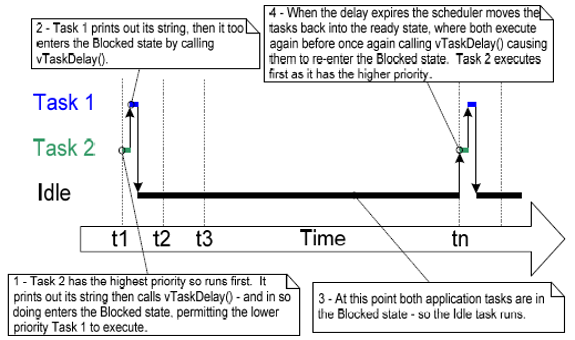
\includegraphics{figures/Fig_6_1_06rtos.png}

\os{\newpage}



\item[{\rot\bf Bold lines indicate the state transitions performed by the tasks in Example 4}]~\\[-3ex]

    \begin{centering}
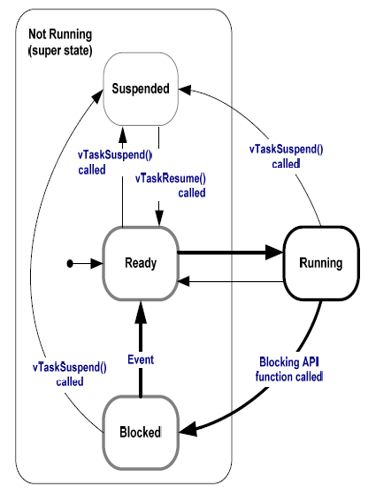
\includegraphics[height=6cm]{figures/Fig_6_1_07rtos.png}
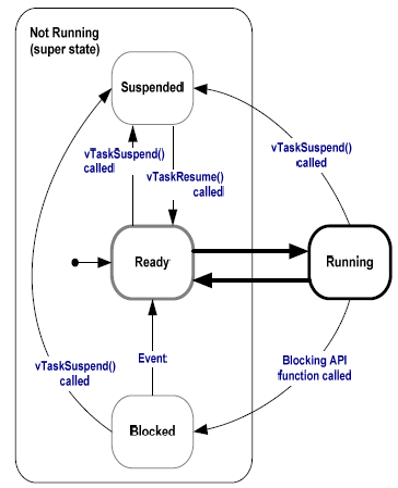
\includegraphics[height=6cm]{figures/Fig_6_1_08rtos.png}
\end{centering}

\bi
\ite Tasks 1+2
\ite Idle Task
\ei

\os{\newpage}



\item[{\rot \bf vTaskDelayUntil() API Function}]~\\[-3ex]

\bi
\ite Parameters to vTaskDelayUntil()
\bi
\ite specify the exact tick count value at which the calling task should be moved from the Blocked state into the Ready state.
\ite Be used when a fixed execution period is required.
\bi
\ite The time at which the calling task is unblocked is absolute rather than relative to when the function was called (as vTaskDelay())
\ei
\ite 	void vTaskDelayUntil(
\ite 		portTickType *pxPreviousWakeTime
\ite 		portTickType xTimeIncrement);
\ei
\ei
\os{\newpage}



\item[{\rot \bf vTaskDelayUntil() prototype}]~\\[-3ex]

\bi
\ite pxPreviousWakeTime
\bi
\ite Assume that vTaskDelayUtil() is being used to implement a task that executes periodically and with a fixed frequency.
\ite Holds the time at which the task left the Blocked state.
\ite Be used as a reference point to compute the time at which the task next leaves the Blocked state.
\ite The variable pointed by pxPreviousWakeTime is updated automatically not be modified by application code other than when the variable is first initialized.
\ei
\ei

\os{\newpage}



\item[{\rot \bf vTaskDelayUntil() prototype}]~\\[-3ex]
\bi
\ite xTimeIncrement
\bi
\ite Assume that vTaskDelayUtil() is being used to implement a task that executes periodically and with a fixed frequency - set by xTimeIncrement.
\ite Be specified in "ticks" . The constant portTICK\_RATE\_MS can be used to convert ms to ticks.
\ei
\ei

\os{\newpage}



\item[{\rot \bf Example 5 Converting the example tasks to use vTaskDelayUntil()}]~\\[-3ex]

\bi
\ite Two tasks created in Example 4 are periodic tasks.
\ite vTaskDelay() does not ensure that the frequency at which they run is fixed
\bi
\ite as the time at which the tasks leave the Blocked state is relative to when they call vTaskDelay().
\ei
\ei

\os{\newpage}



\item[{\rot\bf Example 5 Converting the example tasks to use vTaskDelayUntil()}]~\\[-3ex]
\bi
\ite In void vTaskFunction(void *pvParameters)
\bi
\ite Change
\ite vTaskDelay(250 / portTICK\_RATE\_MS);
\ite // a period of 250ms is being specified.
\ite To
\ite vTaskDelayUntil( \&xLastWakeTime (vTaskDelay(250 / portTICK\_RATE\_MS));
\ite /*xLastWakeTime is initialized with the current tick count before entering the infinite loop. This is the only time it is written to explicitly. */
\ite xLastWakeTime = xTaskGetTickCount();
\ite /*It is then updated within vTaskDelayUntil(); automatically */
\ei
\ei

\os{\newpage}



\item[{\rot\bf Example 6 Combining blocking and non-blocking tasks}]~\\[-3ex]
\bi
\ite Two tasks are created at priority 1.
\bi
\ite Always be either the Ready or the Running state as never making any API function calls.
\ite Tasks of this nature are called continuous processing tasks they always have work to do.
\ei
\ite A Third task is created at priority 2.
\bi
\ite Periodically prints out a string by using vTaskDelayUntil() to place itself into the Blocked state (blocking time 5) between each print iteration.
\ite
\ei
\ei

\os{\newpage}



\item[{\rot\bf Combining blocking and non-blocking tasks}]~\\[-3ex]

\bi
\ite void vContinuousProcessingTask(void * pvParameters) {
\ite   char *pcTaskName;
\ite   pcTaskName = (char *) pvParameters;
\ite   for (;;){ vPrintString(pcTaskName);
\ite         for( ul = 0; ul < 0xfff; ul++ ) { }
\ite   }}
\ite void vPeriodicTask(void * pvParameters) {
\ite   portTickType xLastWakeTime;
\ite   xLastWakeTime = xTaskGetTickCount();
\ite   for (;;){ vPrintString(Periodic task is running);
\ite      vTaskDelayUntil(\&xLastWakeTime
\ite                               (10/portTICK\_RATE\_MS));
\ite   }}
\ei

\os{\newpage}



\item[{\rot\bf Scheduling operations}]~\\[-3ex]

\vspace{2cm}
\begin{centering}
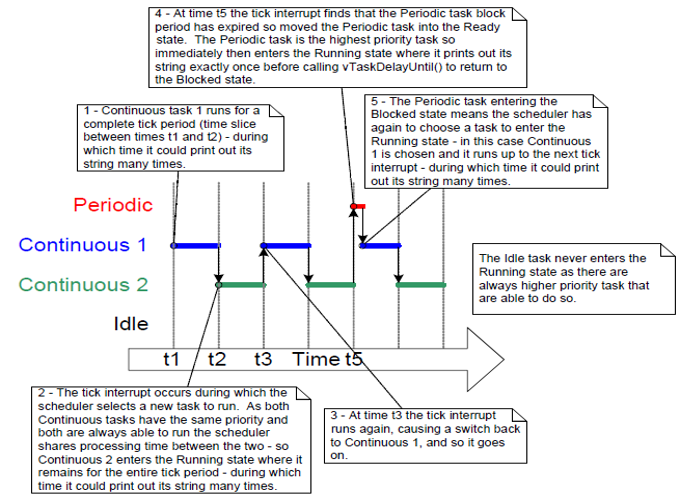
\includegraphics[width = 15 cm]{figures/Fig_6_1_09rtos.png}
\end{centering}
\os{\newpage}



\item[{\rot\bf Idle Task and the Idle task hook}]~\\[-3ex]

\bi
\ite An idle task is automatically created by the scheduler when vTaskStartScheduler() is called.
\bi
\ite Does very little more than site in a loop
\ite Has the lowest possible priority (zero) to ensure it never prevents a higher priority application task from entering the Running state
\ite Be transitioned out of the Running state as soon as a higher priority task enters the Ready state
\ei
\ei

\os{\newpage}



\item[{\rot\bf Idle Task}]~\\[-3ex]

\bi
\ite The Idle task is immediately swapped out to allow Task 2 to execute at the instant Task 2 leaves the Blocked state.
\bi
\ite Task 2 pre-empts the idle task automatically.
\ei
\ei
\begin{centering}
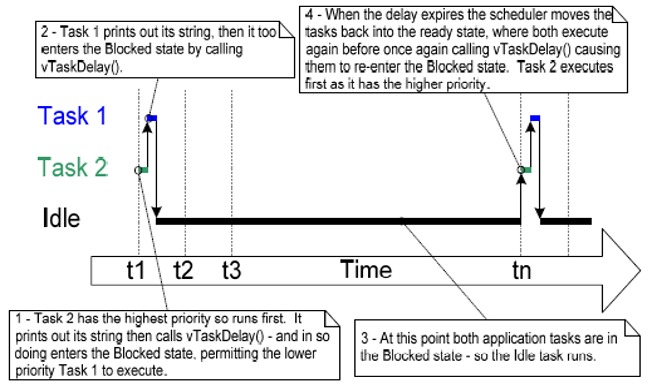
\includegraphics{figures/Fig_6_1_10rtos.png}
\end{centering}
\os{\newpage}



\item[{\rot\bf Idle Task Hook Functions}]~\\[-3ex]

\bi
\ite Add application specific functionality directly into the idle task by the use of an idle hook
\bi
\ite A function called automatically by the idle task once per iteration of the idle task loop
\ei
\ite Common uses for the Idle task hook
\bi
\ite Executing low priority background or continuous processing
\ite Measuring the amount of spare processing capacity
\ite Placing the processor into a low power mode providing an automatic method of saving power whenever no application processing to be performed.
\ei
\ei

\os{\newpage}



\item[{\rot\bf Limitations on the implementation of Idle Task Hook Functions}]~\\[-3ex]

\bi
\ite Rules idle task hook functions must adhere to
\bi
\ite Must never attempt to block or suspend.
\ite If the application uses vTaskDelete() the Idle task hook must always return to its caller within a reasonable time period.
\bi
\ite Idle task is responsible for cleaning up kernel resources after a task has been deleted.
\ite If the idle task remains permanently in the Idle hook function this clean-up cannot occur.
\ei
\ite Idle task hook functions have the name and prototype as
\bi
\ite void vApplicationIdleHook(void);
\ei
\ei
\ei

\os{\newpage}



\item[{\rot\bf Example 7 Defining an idle task hook function}]~\\[-3ex]

\bi
\ite Set configUSE\_IDLE\_HOOK to 1
\ite Add following function
\ite unsigned long ulIdleCycleCount = 0UL;
\ite /* must be called this name take no parameters and return void. */
\ite void vApplicationIdleHook (void) {
\ite    ulIdleCycleCount++;
\ite }
\ite In vTaskFunction() change
\ite 	vPrintString(pcTaskName) To
\ite      vPrintStringAndNumber(pcTaskName ulIdleCycleCount);
\ei

\os{\newpage}



\item[{\rot\bf Idle task and Idle Task Hook}]~\\[-3ex]

\bi
\ite Has the lowest priority possible to add functionality into the idle task vi idle hook
\bi
\ite Execute continuous processing
\ite Measuring spare processing capacity
\ite Placing the processor into a low power mode
\ei
\ite Two rules
\bi
\ite Never block or suspend; must return to its caller within a reasonable time period as it needs to clean up kernel resources after a deleted task.
\ei
\ei

\os{\newpage}



\item[{\rot\bf Change the priority of a task}]~\\[-3ex]

\bi
\ite vTaskPrioritySet(xTaskHandle pxTask unsigned portBASE\_TYPE uxNewPriority);
\ite Be used to change the priority of any task after the scheduler has been started.
\ite Available if INCLUDE\_vTaskPrioritySet  is set 1.
\ei
\ite Two parameters
\bi
\ite pxTask: Handle of the task whose priority is being modified. A task can change its own priority by passing NULL in place of a valid task handle.
\ite uxNewPriority:  the priority to be set.
\ei


\os{\newpage}



\item[{\rot\bf Change the priority of a task}]~\\[-3ex]

\bi
\ite unsigned portBASE\_TYPE uxTaskPriorityGet(xTaskHandle pxTask);
\bi
\ite Be used to query the priority of a task
\ite Available if INCLUDE\_vTaskPriorityGet is set 1
\ite pxTask: Handle of the task whose priority is being modified. A task can query its own priority by passing NULL in place of a valid task handle.
\ite Returned value: the priority currently assigned to the task being queried
\ei
\ei

\os{\newpage}



\item[{\rot\bf Example: Changing task priorities}]~\\[-3ex]

\bi
\ite Demonstrate the scheduler always selects the highest Ready state task to run
\bi
\ite by using the vTaskPrioritySet() API function to change the priority of two tasks relative to each other.
\ei
\ite Two tasks are created at two different priorities.
\bi
\ite Neither task makes any API function calls that cause it to enter the Blocked state
\bi
\ite So both are in either Ready or Running state.
\ite So the task with highest priority will always be the task selected by the scheduler to be in Running state
\ei
\ei
\ei

\os{\newpage}



\item[{\rot\bf Expected Behavior of Example 8}]~\\[-3ex]

\bi
\ite Task 1 is created with the highest priority to be guaranteed to run first. Task 1 prints out a couple of strings before raising the priority of Task 2 to above its own priority.
\ite Task2 starts to run as it has the highest relative priority.
\ite Task 2 prints out a message before setting its own priority back to below that of Task 1.
\ite Task 1 is once again the highest priority task so it starts to run and forcing Task 2 back into the Ready state.
\ei

\os{\newpage}



\item[{\rot\bf Example 8 Continued}]~\\[-3ex]

\bi
\ite Declare a global variable to hold the handle of Task 2.
\bi
\ite xTaskHandle xTask2Handle;
\ei
\ite In main() function create two tasks
\bi
\ite xTaskCreate(vTask1 Task 1 240
\ite 			NULL 2 NULL);
\ite xTaskCreate(vTask2 Task 2 240
\ite 			NULL 1 \&xTask2Handle);
\ei
\ite
\ei

\os{\newpage}



\item[{\rot\bf Initialization}]~\\[-3ex]

\bi
\ite Change vTask1 by initialization
\bi
\ite unsigned portBASE\_TYPE uxPriority;
\ite uxPriority = uxTaskPriorityGet(NULL);
\ei
\ite And adding to the infinite loop
\bi
\ite vTaskPrioritySet(xTaskHandl1 (uxPriority+1));
\ei
\ite Change vTask2 by initialization
\bi
\ite unsigned portBASE\_TYPE uxPriority;
\ite uxPriority = uxTaskPriorityGet(NULL);
\ei
\ite And adding to the infinite loop
\bi
\ite vTaskPrioritySet(NULL (uxPriority-2));
\ei
\ei

\os{\newpage}



\item[{\rot\bf Task with changing priority: execution sequence}]~\\[-3ex]

\vspace{2cm}
\begin{centering}
\includegraphics[height=9 cm]{figures/Fig_6_1_11rtos.png}
\end{centering}

\os{\newpage}



\item[{\rot\bf Deleting a task}]~\\[-3ex]

\bi
\ite Deleted tasks no longer exist and cannot enter the Running state again.
\ite Idle task is responsible to automatically free memory allocated by kernel to tasks that have been deleted.
\bi
\ite Remember if applications use vTaskDelete() do not completely starve the idle task of all processing time.
\ei
\ite Note: any memory or other resource that the application task allocates itself must by be freed explicitly by the application code.
\ei

\os{\newpage}



\item[{\rot\bf vTaskDelete() API function}]~\\[-3ex]

\bi
\ite Function prototype
\bi
\ite void vTaskDelete(xTaskHandle  pxTaskToDelete);
\ite pxTaskToDelete: Handle of the task that is to be deleted. A task can delete itself by passing NULL in place of valid task handle.
\ei
\ite Available only when INCLUDE\_vTaskDelete set 1
\ei

\os{\newpage}



\item[{\rot\bf Example: Deleting tasks (Behavior)}]~\\[-3ex]

\bi
\ite Task 1 is created by main() with priority 1. When it runs it creates Task 2 at priority 2. Task 2 as the highest priority task starts to execute immediately.
\ite Task 2 does nothing but delete itself by passing NULL or its own task handle.
\ite When Task 2 has been deleted Task 1 is again the highest priority task so continues executing - at which point it calls vTaskDelay() to block for a short period.
\ite The idle task executes while Task 1 is in the blocked state and frees the memory that was allocated to the now deleted Task 2.
\ite When Task 1 leaves the blocked state it again becomes the highest priority Ready state task and preempts the Idle task. Then start from Step1 again.
\ei

\os{\newpage}



\item[{\rot\bf Execution sequence}]~\\[-3ex]

\vspace{2cm}
\begin{centering}
\includegraphics[height = 9 cm]{figures/Fig_6_1_12rtos.png}
\end{centering}
\os{\newpage}



\item[{\rot\bf Memory Management}]~\\[-3ex]

\bi
\ite Does not permit memory to be freed once it has been allocated.
\ite Subdivide a single array into smaller blocks. Total size of the array (heap) is set by configTOTAL\_HEAP\_SIZE
\ite xPortGetFreeHeapSize() returns the total amount of heap space that remains unallocated.
\ei

\os{\newpage}



\item[{\rot\bf Heap\_2.c}]~\\[-3ex]

\bi
\ite Allow previously allocated blocks to be freed.
\ite Does not combine adjacent free blocks into a single large block.
\ei

\os{\newpage}



\item[{\rot\bf Summary - Prioritized pre-emptive scheduling}]~\\[-3ex]

\bi
\ite Examples illustrate how and when FreeRTOS selects which task should be in the Running state.
\bi
\ite Each task is assigned a priority.
\ite Each task can exist in one of several states.
\ite Only one task can exist in the Running state at any one time.
\ite The scheduler always selects the highest priority Ready state task to enter the Running state.
\ei
\ei

\os{\newpage}



\item[{\rot\bf Fixed priority Pre-emptive scheduling}]~\\[-3ex]

\bi
\ite Fixed priority
\bi
\ite Each task is assigned a priority that is not altered by the kernel itself (only tasks can change priorities)
\ei
\ite Pre-emptive
\bi
\ite A task entering the Ready state or having its priority altered will always pre-empt the Running state task if the Running state task has a lower priority.
\ei
\ei

\os{\newpage}



\item[{\rot\bf Tasks in the Blocked state}]~\\[-3ex]

\bi
\ite Tasks can wait in the Blocked state for an event and are automatically moved back to the Ready state when the event occurs.
\ite Temporal events
\bi
\ite Occur at a particular time e.g. a block time expires.
\ite Generally be used to implement periodic or timeout behavior.
\ei
\ite Synchronization events
\bi
\ite Occur when a task or ISR sends info to a queue or to one of the many types of semaphore.
\ite Generally be used to signal asynchronous activity such as data arriving at a peripheral.
\ei
\ite
\ei

\os{\newpage}



\item[{\rot\bf Semaphores \& Queues}]~\\[-3ex]

\bi
\ite Introduction to task synchronization
\ite Semaphores and mutexs of FreeRTOS
\ite Queues of FreeRTOS
\ei

\os{\newpage}



\item[{\rot\bf Why Synchronization?}]~\\[-3ex]

\bi
\ite Synchronization may be used to solve:
\bi
\ite Mutual exclusion
\ite Control flow
\ite Data flow
\ei
\ite Synchronization mechanisms include:
\bi
\ite Message queues
\ite Semaphores
\ite Mutexs
\ite Events
\ei
\ite Correct synchronization mechanism depends on the synchronization issue being addressed
\ei


\os{\newpage}



\item[{\rot\bf Mutual Exclusion}]~\\[-3ex]

\bi
\ite Problem: multiple tasks may simultaneously need to access the same resource
\bi
\ite Resource may be code data peripheral etc.
\ite Need to allow the shared resource exclusively accessible to only one task at a time
\ei
\ite How to do?
\bi
\ite Allowing only one task to lock the resource and the rest have to wait for the resource to be unlocked
\ite Common mechanisms: lock/unlock mutex semaphore
\ei
\ei

\os{\newpage}



\item[{\rot\bf Control Flow Synchronization}]~\\[-3ex]

\bi
\ite Problem: a task or ISR may need to resume the execution of one or more other tasks so that tasks execute in an application-controlled order
\bi
\ite Mutual exclusion is used to prevent another task from running while control flow is used to allow another task to run often specific tasks
\ei
\ite How to do?
\bi
\ite Common mechanisms: post/wait signal event
\ei
\ei

\begin{centering}
\includegraphics[height=4cm]{figures/Fig_6_1_13rtos.png}
\end{centering}

\os{\newpage}



\item[{\rot\bf Data Flow Synchronization}]~\\[-3ex]

\bi
\ite Problem: a task or ISR may need to pass some data to one or more other specific tasks so that data may be processed in an application-specified order
\ite How to do?
\bi
\ite May be accomplished indirectly through control flow synchronization
\ite Common mechanisms: queues signal post/wait
\ei
\ei

\os{\newpage}



\item[{\rot\bf Outline}]~\\[-3ex]

\bi
\ite Introduction to task synchronization
\ite Semaphores and mutexs of FreeRTOS
\bi
\ite Binary semaphores
\ite Counting semaphores
\ite Mutex
\ei
\ite Queues of FreeRTOS
\ei

\os{\newpage}



\item[{\rot\bf Semaphores}]~\\[-3ex]

\bi
\ite Semaphores are used to:
\bi
\ite Control access to a shared resource (mutual exclusion)
\ite Signal the occurrence of an event
\ite Allow two tasks to synchronize their activities
\ei
\ite Basic idea
\bi
\ite A semaphore contains a number of tokens. The code needs to acquire one in order to continue execution
\ite If all the tokens of the semaphore are used the requesting task is suspended until some tokens are released by their current owners
\ei
\ei
\includegraphics{figures/Fig_6_1_14rtos.png}

\os{\newpage}



\item[{\rot\bf How Semaphores Work?}]~\\[-3ex]

\bi
\ite A semaphore has:
\bi
\ite Counter: maximum number of concurrent accesses
\ite Queue: for tasks that wait for access
\ei
\ite If a task requests (waits for) a semaphore
\bi
\ite if counter > 0 then (1) the counter is decremented by 1 and (2) task gets the semaphore and proceed to do work
\ite Else task is blocked and put in the queue
\ei
\ite If a task releases (posts) a semaphore
\bi
\ite if there are tasks in the semaphore queue then appropriate task is readied according to queuing policy
\ite Else counter is incremented by 1
\ei
\ei

\os{\newpage}



\item[{\rot\bf Binary Semaphores}]~\\[-3ex]

\bi
\ite Semaphores with counter = 1 used for mutual exclusion and synchronization
\bi
\ite For synchronization purpose a binary semaphore can be think of as a queue that can only hold one item
\bi
\ite The queue can only be empty or full (hence binary)
\ite Tasks using the queue don't care what the queue holds only want to know if the queue is empty or full
\ite  If more than one task blocks on the same semaphore then the task with the highest priority will be the task that is unblocked the next time the semaphore becomes available
\ei
\ei
\ei

\os{\newpage}



\item[{\rot\bf Binary Semaphores and Interrupts}]~\\[-3ex]

\bi
\ite The best way to handle complex events triggered by interrupts is to not do the code in the ISR
\bi
\ite Create a task that is blocking on a binary semaphore
\ite When the interrupt happens the ISR just sets (gives) the semaphore and exits
\ite Task can now be scheduled like any other
\bi
\ite No need to worry about nesting interrupts and interrupt priority
\ei
\ite This is called Deferred Interrupt Processing
\ei
\ei
\os{\newpage}



\item[{\rot\bf Binary Semaphores and Interrupts}]~\\[-3ex]

\bi
\ite Figure from Using the FreeRTOS Real Time Kernel (a pdf book) fair use claimed.
\ei

\begin{centering}
\includegraphics[width = 9 cm]{figures/Fig_6_1_15rtos.png}
\includegraphics[width = 9 cm]{figures/Fig_6_1_16rtos.png}
\end{centering}

\os{\newpage}



\item[{\rot\bf Create a Binary Semaphore}]~\\[-3ex]

\bi
\ite SemaphoreHandle\_t xSemaphoreCreateBinary(void);
\ite Function to create a binary semaphore
\bi
\ite The semaphore is created in the 'empty' state
\ite A binary semaphore need not be given back once obtained so task synchronization can be implemented by one task/interrupt continuously 'giving' the semaphore while another continuously 'takes' the semaphore
\ite Binary semaphores are assigned to variables of type SemaphoreHandle\_t and can be used in any API function that takes a parameter of this type
\ei
\ei

\os{\newpage}



\item[{\rot\bf Set a Binary Semaphore}]~\\[-3ex]

\bi
\ite xSemaphoreGiveFromISR(
\ite   SemaphoreHandle\_t xSemaphore
\ite   signed BaseType\_t *pxHigherPriorityTaskWoken)
\ite Set (give) a semaphore
\bi
\ite Can be used from an ISR
\ite xSemaphore: handle to the semaphore being released
\ite pxHigherPriorityTaskWoken: set to pdTRUE if giving the semaphore caused a task of a higher priority to unblock causing a context switch
\ei
\ei

\os{\newpage}



\item[{\rot\bf Reset a Binary Semaphore}]~\\[-3ex]

\bi
\ite xSemaphoreTake(	xSemaphoreHandle xSemaphore
\ite        	portTickType xBlockTime)
\ite Reset (take) a semaphore
\bi
\ite xSemaphore: handle to the semaphore being taken
\ite xBlockTime: time in ticks to wait for the semaphore to become available
\bi
\ite A block time of zero can be used to poll the semaphore
\ei
\ei
\ei

\os{\newpage}



\item[{\rot\bf Example of Binary Semaphores}]~\\[-3ex]

\vspace{1cm}
\begin{tabular}{|l|} \hline
vSemaphoreHandle binary\_sem; //Global handler
void one\_sec\_isr(void){ // an ISR
  xSemaphoreGiveFromISR(binary\_sem NULL);		
}
void sem\_task(void *p){
  while(1)
    if(xSemaphoreTake(binary\_sem999999)) puts(Tick!);
}
int main(void){
    vSemaphoreCreateBinary(binary\_sem);
    xTaskCreate(sem\_task (signed char*)) t1 2048
         NULL 1 NULL);
    vTaskStartScheduler();
    return 0;	
}  \\ \hline
\end{tabular}


\os{\newpage}



\item[{\rot\bf Counting Semaphores}]~\\[-3ex]

\bi
\ite Typically used for two things:
\ite Counting events:
\bi
\ite An event handler will "give" a semaphore each time an event occurs and a handler task will 'take' a semaphore each time it processes an event
\ei
\ite Resource management:
\bi
\ite The count value indicates number of available resources
\ite To get a resource a task must obtain (take) a semaphore
\ite When a task finishes with the resource it 'gives' the semaphore back
\ei
\ite SemaphoreHandle\_t xSemaphoreCreateCounting( UBaseType\_t uxMaxCount    UBaseType\_t uxInitialCount)
\ei

\os{\newpage}



\item[{\rot\bf Priority Inversion}]~\\[-3ex]

\bi
\ite LPT starts running and acquires the semaphore.
\ite Now HPT is created and it preempts LPT and starts running. It makes the request to acquire the semaphore. Since the semaphore is already with LPT HPT goes to blocked state.
\ite LPT starts executing again and releases the semaphore.
\ite Immediately the HPT comes out of the blocked state and starts executing.
\ite It releases the semaphore and runs for some time and deletes itself.
\ite Now control goes back to LPT which completes its job and deletes itself.
\ite Finally the scheduler is left out with the idle task and it keeps running.
\ei

\os{\newpage}



\item[{\rot\bf Priority Inversion}]~\\[-3ex]

\vspace{1cm}
\begin{centering}
\includegraphics[width=16cm]{figures/Fig_6_1_prio1_rtos}
\end{centering}

\os{\newpage}



\item[{\rot\bf Extended Priority Inversion}]~\\[-3ex]

\bi
\ite LPT starts running and acquires the semaphore.
\ite Now HPT is created and it preempts LPT and starts running. It makes the request to acquire the semaphore. Since the semaphore is already with LPT HPT goes to blocked state.
\ite LPT starts executing again and waits for an event(packet to be received).
\ite Now the Idle task starts running. Now the HPT is starved because of LPT and Idle task.
\ite LPT comes out of blocked state as the event(wait time/packet is received) has occurred. Now it releases the semaphore.
\ite Immediately the HPT comes out of the blocked state and starts executing. It releases the semaphore and runs for some time and deletes itself.
\ite Now control goes back to LPT which completes its job and deletes itself.
\ite Finally the scheduler is left out with the idle task and it keeps running.
\ei

\os{\newpage}



\item[{\rot\bf Extended Priority Inversion}]~\\[-3ex]

\vspace{1cm}
\begin{centering}
\includegraphics[width=16cm]{figures/Fig_6_1_prio2_rtos}
\end{centering}
\os{\newpage}



\item[{\rot\bf Worst Case Priority Inversion}]~\\[-3ex]
\bi
\ite LPT starts running and acquires the semaphore.
\ite Now HPT is created and it preempts LPT and starts running. It makes the request to acquire the semaphore. Since the semaphore is already with LPT HPT goes to blocked state.
\ite LPT starts executing again and creates an MPT tasks.
\ite MPT preempts the LPT and starts running. At this point the HPT is starved because of LPT and MPT. MPT completes its job and deletes itself.
\ite LPT comes out of blocked state and releases the semaphore.
\ite Immediately the HPT comes out of the blocked state and starts executing. It releases the semaphore and runs for some time and deletes itself.
\ite Now control goes back to LPT which completes its job and deletes itself.
\ite Finally the scheduler is left out with the idle task and it keeps running.
\ei

\os{\newpage}



\item[{\rot\bf Worst Case Priority Inversion}]~\\[-3ex]

\vspace{1cm}
\begin{centering}
\includegraphics[width=16cm]{figures/Fig_6_1_prio3_rtos}
\end{centering}
\os{\newpage}



\item[{\rot\bf Priority Inheritance}]~\\[-3ex]
\bi
\ite As soon as the HPT makes a request to semaphore which is allocated to an LPT then the priority of LPT is temporarily increased to that of HPT. Once the LPT releases the semaphore its priority will be restored. Because of this the MPT is never allowed to interfere during the priority inversion(between LPT\&HPT). -> Mutex!
\ite LPT starts running and acquires the semaphore.
\ite Now HPT is created and it preempts LPT and starts running. It makes the request to acquire the semaphore. Since the semaphore is already with LPT HPT goes to blocked state and LPT's priority is temporarily raised to that of HPT.
\ite LPT starts executing again and creates an MPT tasks. It keeps running as its priority is currently higher than MPT. It releases the semaphore and its priority is restored back to lower value.
\ite Immediately the HPT comes out of the blocked state and starts executing.
\ite HPT releases the semaphore and runs for some time and deletes itself.
\ite Now scheduler is left with LPTMPT and IDLE task. MPT starts running and deletes itself after completing its job.
\ite Now control goes back to LPT which completes its job and deletes itself.
\ite Finally the scheduler is left out with the idle task and it keeps running.
\ei

\os{\newpage}



\item[{\rot\bf Priority Inheritance}]~\\[-3ex]

\vspace{1cm}
\begin{centering}
\includegraphics[width=16cm]{figures/Fig_6_1_prio4_rtos}
\end{centering}
\os{\newpage}



\item[{\rot\bf Mutex}]~\\[-3ex]
\bi
\ite Mutexes are used for mutual exclusion so that only one task at a time uses a shared resource e.g. file data device ...
\bi
\ite To access the shared resource a task locks the mutex associated with the resource
\ite The task owns the mutex until it unlocks the mutex
\ei
\ei
\includegraphics[width=16cm]{figures/Fig_6_1_17rtos.png}

\os{\newpage}



\item[{\rot\bf Mutex}]~\\[-3ex]
\bi
\ite Mutex acts like a token used to guard a resource
\bi
\ite When a task wishes to access the resource it must first obtain ('take') the token
\ite When the task has finished with the resource it must 'give' the token back - allowing other tasks the opportunity to access the same resource
\ei
\ite Mutexes are binary semaphores that include a priority inheritance mechanism
\bi
\ite If a high priority task blocks while attempting to obtain a mutex (token) that is currently held by a lower priority task then the priority of the task holding the token is temporarily raised to that of the blocking task
\ei
\ei

\os{\newpage}



\item[{\rot\bf Priority Inversion}]~\\[-3ex]
\bi
\ite Assume priority of T1 \> priority of T9
\bi
\ite If T9 has exclusive access T1 has to wait until T9 releases resource inverting priority can raise priority of T9
\ei
\ei
\includegraphics[width=14cm]{figures/Fig_6_1_18rtos.png}
\bi
\ite T1 has higher priority and preempts T9
\ei
\bi
\ite Critical section
\ei
\bi
\ite (critical section)
\ei

\os{\newpage}



\item[{\rot\bf Example of Mutex (1/3)}]~\\[-3ex]

\vspace{1cm}
\begin{tabular}{|l|} \hline
xSemaphoreHandle gatekeeper = 0; //Global handler\\

void task\_1(void *p)\{\\
  while(1)\{\\
    if(xSemaphoreTake(gatekeeper 1000))\{\\
      puts(Task 1 got access);\\
	access\_precious\_resource(); // critical section\\
	xSemaphoreGive(gatekeeper);  \}\\
    else\{\\
	puts(Task 1 failed to get access within 1000ms);\\
    \}\\
    vTaskDelay(1000);\\
      /*Without delay Task 1 will get key immediately\\
          after releasing the key */ \\
  \}\\
\}  \\ \hline
\end{tabular}


\os{\newpage}



\item[{\rot\bf Example of Mutex (2/3)}]~\\[-3ex]

\vspace{1cm}
\begin{tabular}{|l|} \hline
void task\_2(void *p)\{ \\
  while(1)\{\\
    if(xSemaphoreTake(gatekeeper 1000))\{ \\
      puts(Task 2 got access);\\
	access\_precious\_resource(); // critical section\\
	xSemaphoreGive(gatekeeper); \}\\
    else\{\\
	puts(Task 2 failed to get access within 1000ms);\\
    \}\\
    vTaskDelay(1000);\\
    /*Without delay task 2 will get key immediately\\
          after releasing the key */\\
   \}\\
\}  \\ \hline
\end{tabular}


\os{\newpage}



\item[{\rot\bf Example of Mutex (3/3)}]~\\[-3ex]

\vspace{1cm}
\begin{tabular}{|l|} \hline
int main(void)\{\\
  gatekeeper = xSemaphoreCreateMutex();\\
\\
  /*Create tasks with priority 1 for both users*/\\
  xTaskCreate(task\_1 (signed char*)) t1 1024\\
      NULL 1 NULL);\\
  xTaskCreate(task\_2 (signed char*)) t2 1024\\
      NULL 1 NULL);\\
	\\
  vTaskStartScheduler();\\
  return 0;\\
\}  \\ \hline
\end{tabular}


\os{\newpage}



\item[{\rot\bf Outline}]~\\[-3ex]
\bi
\ite Introduction to task synchronization
\ite Semaphores and mutexs of FreeRTOS
\ite Queues of FreeRTOS
\ei

\os{\newpage}



\item[{\rot\bf FreeRTOS Queues}]~\\[-3ex]

\bi
\ite Queues are the primary form of inter-task communications in FreeRTOS
\bi
\ite Can be used to send messages between tasks and between interrupts and tasks
\ite In most cases used as thread safe FIFO (First In First Out) buffers with new data being sent to the back of the queue although data can also be sent to the front.
\ei
\ei
\includegraphics[width=16cm]{figures/Fig_6_1_19rtos.png}

\os{\newpage}



\item[{\rot\bf FreeRTOS Queues}]~\\[-3ex]

\bi
\ite Queues store a finite number of fixed-size data
\bi
\ite May be read and written by different tasks but do not belong to any task
\ite \# of items and item size determined at queue create time
\ite Sending/receiving items are by copy not reference
\ei
\ite Queue functions
\bi
\ite Create queues: xQueueCreate() vQueueDelete()
\ite Send/receive data to/from queues: xQueueSend() xQueueSendToBack() xQueueReceive() xQueueReceiveFromISR()
\ite Queue management/number of items in a queue
\ite Blocking on a queue/effect of priority
\ei
\ei

\os{\newpage}



\item[{\rot\bf Blocking on Queues}]~\\[-3ex]

\bi
\ite Queue APIs permit a block time to be specified
\ite When read from an empty queue
\bi
\ite Task will be placed into the Blocked state
\ite Until data is available on the queue or block time expires
\ei
\ite When write to a full queue
\bi
\ite Task will be placed into the Blocked state
\ite Until space is available in the queue or block time expires
\ei
\ite If more than one task block on the same queue then the task with the highest priority will be the task that is unblocked first
\ei

\os{\newpage}



\item[{\rot\bf Queue Creation}]~\\[-3ex]

\bi
\ite QueueHandle\_t xQueueCreate(
\ite     UBaseType\_t uxQueueLength
\ite     UBaseType\_t uxItemSize);
\ite Creates a new queue instance
\bi
\ite Allocates queue storage and returns a handle
\ite uxQueueLength: maximum number of items that the queue can contain
\ite uxItemSize: number of bytes that each item in the queue will require
\bi
\ite Items are queued by copy not by reference so this is the number of bytes that will be copied for each posted item
\ei
\ite Each item on the queue must be the same size
\ei
\ei

\os{\newpage}



\item[{\rot\bf Send Data through Queues}]~\\[-3ex]

\bi
\ite BaseType\_t xQueueSend(QueueHandle\_t xQueue
\ite       const void * pvItemToQueue
\ite       TickType\_t xTicksToWait);
\ite Post an item on a queue
\bi
\ite The item is queued by copy not by reference
\ite Must not be called from an interrupt service routine
\ite xQueue:  queue handle to which the item is to be posted
\ite pvItemToQueue: pointer to item to be placed on queue
\ite xTicksToWait: max. time (in ticks) that task should block waiting for space to become available should it is full
\ite If INCLUDE\_vTaskSuspend is set to "1" then specifying the block time as portMAX\_DELAY will block task indefinitely
\ei
\ei

\os{\newpage}



\item[{\rot\bf Receive Data through Queues}]~\\[-3ex]

\bi
\ite BaseType\_t xQueueReceive(
\ite     QueueHandle\_t xQueue void *pvBuffer
\ite     TickType\_t xTicksToWait);
\ite Receive an item from a queue
\bi
\ite The item is received by copy so a buffer of adequate size must be provided
\ite Must not be used in an interrupt service routine
\ite xQueue: queue handle from which to receive item
\ite pvBuffer: pointer to the buffer into which the received item will be copied.
\ite xTicksToWait: max. amount of time the task should block waiting for an item should the queue be empty
\ei
\ei

\os{\newpage}



\item[{\rot\bf Example of Queues (1/2)}]~\\[-3ex]

\vspace{1cm}
\begin{tabular}{|l|} \hline
xQueueHandle Global\_Queue\_Handle = 0; //Global Handler\\
void sender\_task(void *p)\{  int i=0;\\
  while(1)\{\\
    printf(Send %i to receiver task i);\\
    if(!xQueueSend(Global\_Queue\_Handle \&i 1000))\\
      printf(Failed to send to queue);		\\
    i++;\\
    vTaskDelay(3000);   \}\\
\}\\
void receiver\_task(void *p)\{\\
  int rx\_int = 0;\\
  while(1)\{\\
    if(xQueueReceive(Global\_Queue\_Handle \&rx\_int1000))\\
	   printf(Received %i rx_int);\\
    else puts(Failed to receive data from queue);  \}\\
\}  \\ \hline
\end{tabular}


\os{\newpage}



\item[{\rot\bf Example of Queues (2/2)}]~\\[-3ex]

\vspace{1cm}
\begin{tabular}{|l|} \hline
int main(void)\{\\
\\
  Global\_Queue\_Handle = xQueueCreate(3 sizeof(int));\\
\\
  /*Create tasks with priority 1 for both users*/\\
   xTaskCreate(sender\_task (signed char*)) sx\\
      1024 NULL 1 NULL);\\
   xTaskCreate(receiver\_task (signed char*)) rx\\
       1024 NULL 1 NULL);\\
	\\
   vTaskStartScheduler();\\
   return 0;\\
\}  \\ \hline
\end{tabular}


\os{\newpage}



\end{description}

%%%%%%%%%%%%%%%%%%%%%%%%%%%%%%%%%%%%%%%%%%%%%%%%%%%%%%%%%%%%%%%%%%%%%%%%%%%
\section{Functions of Embedded Linux}
%%%%%%%%%%%%%%%%%%%%%%%%%%%%%%%%%%%%%%%%%%%%%%%%%%%%%%%%%%%%%%%%%%%%%%%%%%%
\bi
	\ite the general idea of an ``embedded Linux'' is to store an image (Kernel plus necessary modules) in a non-volatile memory (Flash-EEPROM, SD-Card).
	\ite after a reset (or power on reset) the image is copied in the RAM and executed.
	\ite the size of the copied image is also known as a ``footprint''.
	\ite the additional feature of embedded CLinux (Linux for microcontrollers) is has the opportunity to work without a virtual memory system (VM).
	\bi
		\ite suitable for processors without MMU.
		\ite low memory footprint.
		\ite according to the processors low power consumption applications are possible.
	\ei
	\bigskip
	\ite with the ARM-Processors (MMU is available)  embedded Linux could run with a virtual memory system or with a non virtual memory system.
\ei
\os{\newpage}
\begin{description}
\item[{\rot\bf Boot sequence}]~\\[-3ex]
\bigskip
\bi
	\ite the boot procedure of embedded Linux differs from a standard boot procedure.
	\ite this procedure offers two advantages:
	\bi
		\ite the development process of building a Linux system is nearly the same as in a standard Linux (the same tools are available).
		\ite the execution time of programs which runs in a RAM is much more faster than in a Flash-EPROM).
	\ei
	\bigskip
	\ite boot procedure starts immediately after the reset (an interaction with the user isn't necessary).
\ei
\os{\newpage}
\begin{figure}[!hbtp]
     \begin{center}
	  \epsfig{file=figures/Fig_6_2_Boot,width=0.4\textwidth}\\
	  \caption{Boot Procedure}
     \end{center}
\end{figure}
\os{\newpage}

\item[{\rot\bf Scalable behaviour of embedded Linux}]~\\[-3ex]
\bi
	\ite building of a new image (binaries of embedded Linux systems) starts with a configuration part.
	\ite first part is the selection of the ``vendor''.
	\ite specification of hardware details of the development kit (RAM addresses, ROM addresses).
	\ite the next step is the configuration of necessary modules and drivers.

\ei

\os{\newpage}
\begin{figure}[!hbtp]
     \begin{center}
	  \epsfig{file=figures/Fig_6_3_Vendor,width=0.8\textwidth}\\
	  \caption{Specification of Hardware Details}
     \end{center}
\end{figure}
\os{\newpage}
\begin{figure}[!hbtp]
     \begin{center}
	  \epsfig{file=figures/Fig_6_4_Drivers,width=0.8\textwidth}\\
	  \caption{Configuration through a Selection of Moduls or Drivers}
     \end{center}
\end{figure}
\os{\newpage}

\item[{\rot\bf Build procedure}]~\\[-3ex]
\bi
	\ite after the configuration (make menuconfig)
	\bi
		\ite start the build process with ``make dep''.
		\ite  and ``make''.
	\ei
	\bigskip
	\ite the Kernel-compilation need a special compiler (gcc-version for the ARM-Processor) und a special binutils (as, ld objtools for the ARM-Processor).
	\ite the result of the Kernel-compilation is a image which is available in two versions.
	\bi
		\ite file ``linux.bin or Kernel.img'' .
		\bi
			\ite a loadable image.
			\ite could be downloaded (serial or usb-interface, needs a monitor program on the target side ).
			\ite execute after a poweron reset or with a jump on a specific address (monitor function).
			\ite useful for test of a configuration.
		\ei
		\bigskip
		\ite file ``romfs''
		\bi
  			\ite a image which could be loaded in the FlashEPROM.
			\ite need a ``Flash''-load program like CF-Flasher.
			\ite embedded Linux starts after the next reset or power-on-reset with the mentioned boot sequence.
		\ei
	\ei
\ei

\item[{\rot\bf Working with embedded Linux in the target}]~\\[-3ex]

\bi
	\ite establish a serial communication link between the target and the PC.
	\bi
		\ite works as standard input/output (stdio) for messages from embedded Linux.
		\ite on the PC-side, a terminal program like ``minicom''  for Linux or ''Hyperterminal'' for Windows is useful.
	\ei
\ei
\os{\newpage}
\begin{figure}[!hbtp]
     \begin{center}
	  \epsfig{file=figures/Fig_6_5_Minicom,width=0.8\textwidth}\\
	  \caption{Serial Communication Tool Minicom}
     \end{center}
\end{figure}

\os{\newpage}
\begin{figure}[!hbtp]
     \begin{center}
	  \epsfig{file=figures/Fig_6_5_Minicom_P,width=0.6\textwidth}\\
	  \caption{Configuration of Minicom}
     \end{center}
\end{figure}

\os{\newpage}
\bi
	\ite if an ethernet link is established
	\bi
	  \ite generate a remote connection (via ssh)
	  \bi
	    \ite execution of commandline instructions on the target
	  \ei
	  \ite mount PC partition by NFS
	  \bi
	    \ite target-filesystem can be mounted in the development-filesystem
	    \ite execute programs on the development-side and on the target-side
	  \ei
	\ei
\ei
\begin{figure}[!hbtp]
     \begin{center}
	  \epsfig{file=figures/Fig_6_6_uCLinux,width=0.9\textwidth}\\
	  \caption{Standard Commandline Interface on the Target-side}
     \end{center}
\end{figure}

\os{\newpage}
\item[{\rot\bf Restrictions when using non VM-systems}]~\\[-3ex]
\bigskip
\bi
	\ite ARM-Processors could operate with a VM (virtual memory) and a non VM System.
	\ite in the case of working without a VM-System:
	\bi
		\ite a user program has full access to the whole memory space.
		\ite as a result, no segmentation fault is possible.
		\ite no dynamic heap \pr instead uCLinux uses a global memory pool (kernel free memory pool).
		\ite no obvious implementation of malloc due to lack of heap.
		\ite no fork sytem call \pr an implementation of ``copy on write'' strategy isn't possible (an alternative is the old BSD vfork and all its limits).
	\ei
\ei
\end{description}

%%%%%%%%%%%%%%%%%%%%%%%%%%%%%%%%%%%%%%%%%%%%%%%%%%%%%%%%%%%%%%%%%%%%%%%%%%%
\section{Cross Compilation}
%%%%%%%%%%%%%%%%%%%%%%%%%%%%%%%%%%%%%%%%%%%%%%%%%%%%%%%%%%%%%%%%%%%%%%%%%%%
\bi
	\ite cross compilation is widely used for programming in embedded systems.
	\ite the programs are written, linked and simulated on a PC (for example) for an embedded system.
	\ite then these executable programs have to be downloaded and started on the target under the control of a monitor program (mostly with a serial connection between the PC and the target).
	\ite after the test in the target the executable program could be stored in the EPROM and executed without a monitoring program
\ei
\os{\newpage}
\begin{figure}[!hbtp]
     \begin{center}
	  \epsfig{file=figures/Fig_6_7_CrossCompilation,width=0.9\textwidth}\\
	  \caption{Cross Compilation}
     \end{center}
\end{figure}

\os{\newpage}
\begin{description}
\item [{\rot\bf Cross compilation with embedded Linux}]~\\[-3ex]
\bigskip
\bi
	\ite in embedded Linux systems the cross compilation is done for the same reasons as for a standard system.
	\ite the advantage in this case is that the same debugging tools that are available for the test on the PC are also available on tests on the target system (remote debugging).
	\bigskip
	\ite to compile a program for the ARM-Processor a specific toolchain is necessary
	\ite the same toolchain is also used to build the embedded Linux System for the target.
	\ite to generate all parts of the toolchain the standard C-compiler and C-libraries are also involved:
\ei
\os{\newpage}
\begin{center}
 \begin{tabular}{|l|l|}
\hline
Tool & Description\\
\hline
arm-linux-gcc & C-Compiler for ARM-Processor\\
\hline
arm-linux-as & Assembler for ARM-Processor\\
\hline
arm-linux-ld & Linker for ARM-Processor\\
\hline
\hline
arm-linux-ar & Archiver, tool to build, extract and show the contents \\  & of libraries \\
\hline
arm-linux-nm & extracts the symbols of an executable file\\
\hline
arm-linux-objdump & extract the contents of an executable file \\
 & (e.g. disassemble files)\\
\hline
arm-linux-objcopy & tool to generate loadable files from \\
 & the output of the linker (e.g. ``x.bin'' or ``x.ihex'') \\
\hline
 \end{tabular}
\end{center}
\os{\newpage}
\item [{\rot\bf Executable files}]~\\[-3ex]	
\bigskip
\bi
	\ite standard output of the linker (``x.elf'') isn't downloadable.
	\bi
		\ite this file needs a VM-System for loading and execution.
	\ei
	\bigskip
	\ite instead of ``x.elf'' the tool arm-linux-objcopy generates a ``x.bin'' and/or ``x.ihex''-file.
	\bi
		\ite both files are directly downloadable and don't need a VM-System for execution.
		\ite this means both file are linked on an absolute address.
		\ite the ``x.bin''-format is a binary format (could not be read with an editor).
		\ite the ``x.ihex''.format is a text format which is readable with any standard editor.
	\ei
\ei
\os{\newpage}
\begin{figure}[!hbtp]
     \begin{center}
	  \epsfig{file=figures/Fig_6_8_Info_ELF,width=0.9\textwidth}\\
	  \caption{Information in a ``x.elf''-file}
     \end{center}
\end{figure}



\end{description}
%%%%%%%%%%%%%%%%%%%%%%%%%%%%%%%%%%%%%%%%%%%%%%%%%%%%%%%%%%%%%%%%%%%%%%%%%%%
\section{User Programming in uCLinux}
%%%%%%%%%%%%%%%%%%%%%%%%%%%%%%%%%%%%%%%%%%%%%%%%%%%%%%%%%%%%%%%%%%%%%%%%%%%	
\bi
	\ite user programming implies that a program runs in the user mode of the ARM-Processor.
	\ite if the VM-System is activated \pr the user doesn't have an access to an absolute memory address.
	\bi
		\ite especially a direct access to the registers of interfaces isn't allowed.
	\ei
	\bigskip
	\ite the restrictions imply also that an access to R-, S-, D-registers, CPSR and etc. are not allowed.
	\ite these access could only be done in the supervisor mode (kernel program).
\ei
\bigskip
\bi
	\ite Development of program should be done in tree steps:
	\bi
           \ite first try to generate a program with a cross-compilation for the target, load and then test it.
	      \ite then merge the program together with an image of the operating system and load it.
	      \ite lastly, if necessary implement a "autoexec" function in the init process of the embedded Linux.
      \ei
\ei
\begin{description}
\item[{\rot\bf Cross-compilation with embedded Linux}]~\\
\bi
	\ite the cross-compilation with embedded Linux has the same procedure as the standard cross-compilation for ARM-Processors.
	\ite in preparation for the next two steps it is helpful to use a separate directory which holds all the necessary files (C-files, Header-files, makefile).
	\ite put this directory in the ARM-Linux-file-system '/armLinux/user/' .
	\ite after the compilation mount the directory with NFS in the uCLinux for the target and execute and test the program.
\ei
\bigskip
\item[{\rot\bf Download together with an image of  embedded Linux}]~\\
\bi
	\ite the second step is to integrate the program in an image of uCLinux.
	\ite additional to the cross-compilation, the program also has to be integrated in the build procedure of uCLinux.
	\bi
		\ite the ``central''-makefile for building all the user applications \\ (/armLinux/user/makefile) should expanded with an instruction like:
		\\ \begin{tabular}{l l l l}
		    DIRSc\$(CONFIG\_USER\_CAN)& += & can4linux & (present line)\\
		    DIRSc\$(CONFIG\_USER\_PROGRAM)& += & program & (new line)\\
		   \end{tabular}
		\ite to make the program visible in configuration tool (make menuconfig) of armLinux the file 'config.in' (/armLinux/user/config.in) should expand by:
		\\ \begin{tabular}{l l l}
		    bool 'can4linux' & CONFIG\_USER\_CAN & (present line) \\
		    bool 'program' & CONFIG\_USER\_PROGRAM & (new line) \\
		   \end{tabular}
		\ite to get some more information about the program and how somebody can do the configuration the file Configure.help \\
		(/armLinux/user/Documentation/Configure.help) should expand by
		\\ \begin{tabular}{l l}
		   CONFIG\_USER\_CAN& \\
		    & This package contains some examples\\
		    & using can4linux device driver.\\
		    & \\
		   CONFIG\_USER\_PROGRAM& \\
		    & This programm adds my first functions \\
		    & to uCLinux. I'm not sure whether \\
		    & somebody can use these functions.\\
		   \end{tabular}
		\os{\newpage}
		\ite if in the configuration step, the program is selected, the resulting image contains the program
		\ite to test the image (armLinux) and the program once more, it can be downloaded with the monitor
		\ite the downloaded armLinux (including the program) could be started after a reboot or a reset
	\ei
\os{\newpage}
\ei
\item[{\rot\bf Autostart of a program with embedded Linux}]~\\
\bi
	\ite if the program (which was downloaded together with the armLinux-image) has to be used, the user has to start it.
	\ite embedded Linux offers an automatic start of programs (function of the program init which execute the sript file /etc/inittab).
	\ite the sript-file inittab ask an another skript-file rcS (placed in /etc/rc.d/rcS) and this file switch over to rc.local (/etc/rc.d/rc.local).
	\ite an auto start could be done by addition in the file rc.local (but this means that the user has to change this file and this is obviously not an autostart, escpecially not for the first time).
	\ite to do a 'real' auto start of the file \\
	/armLinux/defconfigs/vendors/senTec/etc/rc.d/rc.local has to changed and then a new image has to be created.
	\ite when this image is loaded in the FlushEPROM (with the program CFFlusher) then after a reset the program is automatical started without an interaction with the user.
\ei

%\os{\newpage}
%\item[{\rot\bf Applications for ARM Cortex on a BeagleBoard or a Rasberry Pi Board}]~\\
%\begin{center}
%\begin{tabular}{|l|l|}
%\hline
%Exercice 1 & \textbf{BeagleBoard: Digital I/O} \\
%\hline
%Participants & Ramachandran, Mahalinam; Amar, Jadhav \\
%\hline
%Presentation & Mo. 24.6.2013, 16.00 \\
%\hline
%\hline
%Exercice 2 & \textbf{BeagleBoard: Set up an Eclipse-based } \\
%	   & \textbf{Cross Compilation} \\
%\hline
%Participants & Jamshid, Ummattam; Archana, Basavalingappa; \\
%	     & Sharath, Chandra \\
%\hline
%Presentation & Wed. 24.6.2013, 16.15 \\
%\hline
%\hline
%Exercice 3 & \textbf{BeagleBoard: Use  GPIO and a external} \\
%	   & \textbf{D/A-Converter to build a Function Generator} \\
%\hline
%Participants & MD. Arifur Rahman, Neecati, Gouthan \\
%\hline
%Presentation & Wed. 24.6.2013, 16.30 \\
%\hline
%\end{tabular}
%\end{center}



\end{description} 

%%%%%%%%%%%%%%%%%%%%%%%%%%%%%%%%%%%%%%%%%%%%%%%%%%%%%%%%%%%%%%%%%%%%%%%%%%


%%%%%%%%%%%%%%%%%%%%%%%%%%%%%%%%%%%%%%%%%%%%%%%%%%%%%%%%%%%%%%%%%%%%%%%%%%



%%% Local Variables:
%%% mode: latex
%%% TeX-master: "docu"
%%% End:



\newpage
\baselineskip 5mm
\def\refname{Literatur}
\bibliography{refs}
\addcontentsline{toc}{chapter}{References}
\end{document}
